% $Id$
%%%%%%%%%%%%%%%%%%%%%%%%%%%%%%%%%%%%%%%%%%%%%%%%%%%%%%%%%%%%%%%%%%%%%%

\documentclass[a4paper,11pt,oneside]{book}
\overfullrule=5pt
\usepackage[latin1]{inputenc}
\DeclareTextSymbolDefault{\dh}{T1}
\DeclareTextSymbolDefault{\textperthousand}{T1}

\usepackage{datetime} % To distinguish often compiled draft versions

\setlength{\fboxrule}{.5mm}
\setlength{\fboxsep}{1.75mm}
\setlength{\footnotesep}{6pt}

\usepackage{amsmath}
\usepackage{amssymb,amscd,latexsym}   %BERM2: added for biciphers.tex
\usepackage{amsfonts}
\usepackage{amsthm}
\usepackage{color}

\usepackage{fancyvrb}
\usepackage{makeidx}
\usepackage[pdftex]{graphicx}
\usepackage{pdfpages}
\usepackage{paralist}
\usepackage{arydshln}
\usepackage{verse}

\usepackage[flushmargin]{footmisc}
\usepackage{fullpage}
\usepackage[hyphens]{url}
\appto\UrlBreaks{\do\a\do\b\do\c\do\d\do\e\do\f\do\g\do\h\do\i\do\j
\do\k\do\l\do\m\do\n\do\o\do\p\do\q\do\r\do\s\do\t\do\u\do\v\do\w
\do\x\do\y\do\z}

\usepackage[labelstoglobalaux]{bibunits}
%\bibliographyunit[\section] % bibunits f�r das ganze Dokument aktivieren
\defaultbibliography{references} % Why only in English version?
\defaultbibliographystyle{abbrv} % Why only in English version?

\usepackage{float}
\usepackage{subfig}
\usepackage{shorttoc}
\usepackage[colorlinks=true,linkcolor=black,citecolor=black,urlcolor=black,bookmarksnumbered=true,pdfpagelabels,plainpages=false,hyperfootnotes=false]{hyperref}

\floatstyle{boxed}
\newfloat{ctsquotefloat}{H}{loq}
\floatname{ctsquotefloat}{Quote}
\newenvironment{ctsquote}{\begin{ctsquotefloat}\center}{\end{ctsquotefloat}}
\floatstyle{ruled}

\newfloat{sagecode}{!ht}{loc}[chapter]
\floatname{sagecode}{SageMath sample}

\newfloat{cryptoprocedure}{!ht}{lop}[chapter]
\floatname{cryptoprocedure}{Crypto Procedure}


\makeindex
\hypersetup{colorlinks=true}

%\newcommand{\href}[2]{#2}
\newcommand{\hypertag}[2]{#1}
%\newcommand{\hyperlink}[2]{#2}
%\newcommand{\hypertarget}[2]{#2}

\newtheorem{definition}{Definition}[section]
\newtheorem{theorem}{Theorem}[section]
\renewenvironment{proof}[1]{\noindent\textbf{Proof #1} \\}{\hfill$\Box$\par}  %BERM: Instead of making AMS-Theorem a comment in order to have no redefinition of proof, used renewenvironment [proof used in moderncryptography.text and primes.text]. Necessary only in English!
\newenvironment{example}[1]{\noindent\textbf{Example#1}}{}
\newenvironment{remark}[1]{\noindent\textbf{Comment#1}}{}

\newenvironment{ Latex_Create-Closed-Dummy-Environ }{}{}

\setcounter{tocdepth}{4}
\setcounter{secnumdepth}{4}


% Define title ..............
\title{ % Keine Leerzeilen, sonst Meldung: "Paragraph ended before \title was complete."
	{\Huge The CrypTool Book \\[15pt]
         Cryptography, Mathematics, and More} \\[25pt]
	{\LARGE	Background reading for CrypTool\\ 
         the free e-learning crypto program \\[5pt]
	 (with code samples written in SageMath)} \\[25pt]
	{\large 12th edition -- draft version (\settimeformat{hhmmsstime}\currenttime)}
	% {\large 12th edition}
        \vspace{180pt}
}

\author{
        {\LARGE Prof.\ Bernhard Esslinger (co-author and editor)}\\[10pt]
        {\LARGE and the CrypTool Team, 1998-2016}\\[10pt]
        {\LARGE Frankfurt am Main, Germany} \\*[15pt]
        \url{www.cryptool.org}
}


%%%%%%%%%%%%%%%%%%%%%%%%%%%%%%%%%%%%%%%%%%%%%%%%%%%%%%%%%%%%%%%%%%%%
\begin{document}
\VerbatimFootnotes

% \includepdf[pages=1]{figures/coverv1_en-300dpi.pdf}
% \includepdf[pages=1]{figures/coverv1_en.pdf}
\includepdf[pages=1]{figures/coverv1_en_draft.pdf}

\frontmatter

\pagestyle{plain}
\setlength{\fboxrule}{.5mm}
\setlength{\fboxsep}{1.75mm}
\setlength{\footnotesep}{6pt}
\addtolength{\footskip}{8pt}

\renewcommand\footnoterule{%
  \vspace{2em}
  \hrule width .4\columnwidth
 \vspace{4pt}
}

\maketitle


\begin{quote}
This is a free document, so the content of the document can
be copied and distributed, also for commercial purposes --- as long as
the authors, title and the CrypTool web site (\url{www.cryptool.org})
are acknowledged. Naturally, citations from the CrypTool script are
possible, as in all other documents.\\
Additionally, this document is liable to the specific license of the
GNU Free Documentation Licence.

    Copyright \copyright{} 1998--2016 Bernhard Esslinger and the
    CrypTool Team. Permission is granted to copy,
    distribute and/or modify this document under the terms of the GNU
    Free Documentation License, Version 1.3 or any later version
    published by the Free Software Foundation. A copy of
    the license is included in the section entitled
    \hyperlink{appendix-GNU-fdl}{``GNU Free Documentation License''}.

    This also includes the code of the SageMath samples in this document.
\end{quote}

\vspace{420pt}
\noindent
Source cover photograph: \url{www.photocase.com}, Andre Guenther\\
Typesetting software: \LaTeX\\
Version control software: Subversion


% $Id$
% ............................................................................
%                 TEXT DER 2. SEITE
% ~~~~~~~~~~~~~~~~~~~~~~~~~~~~~~~~~~~~~~~~~~~~~~~~~~~~~~~~~~~~~~~~~~~~~~~~~~~~
% --------------------------------------------------------------------------
% HACK to fix warning "destination with the same identifier .. has already been used, ...":
\makeatletter \renewcommand{\thepage}{~\csname @roman\endcsname \c@page~} \makeatother
\clearpage\phantomsection
% HACK to fix warning "destination with the same identifier .. has already been used, ...":
\makeatletter \renewcommand{\thepage}{\csname @roman\endcsname \c@page} \makeatother
\addcontentsline{toc}{chapter}{�berblick}
\chapter*{�berblick �ber den Inhalt des CrypTool-Skripts}

\parskip 4pt
%\vskip +12 pt
In diesem {\em Skript zu dem Programm CrypTool} \index{CrypTool} finden Sie
eher mathematisch orientierte Informationen zum Einsatz von
kryptographischen Verfahren. Zu einigen Verfahren gibt es Beispielcode,
geschrieben f�r das Computer-Algebra-System {\bf Sage}\index{Sage}
(siehe Anhang~\ref{s:appendix-using-sage}).
Die Hauptkapitel sind von verschiedenen {\bf Autoren} verfasst
(siehe Anhang~\ref{s:appendix-authors}) %\hyperlink{appendix-authors}{Autoren}
und in sich abgeschlossen. Am Ende der meisten Kapitel finden Sie
jeweils Literaturangaben und Web-Links.

Das \hyperlink{Kapitel_1}{erste Kapitel} beschreibt die Prinzipien der
symmetrischen und asymmetrischen {\bf Verschl�sselung} und erl�utert 
kurz die aktuellen Entschl�sselungsrekorde bei modernen symmetrischen
Verfahren.

Im \hyperlink{Kapitel_PaperandPencil}{zweiten Kapitel} wird -- aus 
didaktischen Gr�nden -- eine ausf�hrliche �bersicht
�ber {\bf Papier- und Bleistiftverfahren} gegeben.

Ein gro�er Teil des Skripts ist dem faszinierenden Thema der
{\bf Primzahlen} (Kapitel \ref{Label_Kapitel_Primes})
% \hyperlink{Kapitel_2}{{\bf Primzahlen}} 
gewidmet.
Anhand vieler Beispiele bis hin zum {\bf RSA-Verfahren} wird in die
{\bf modulare Arithmetik} und die 
{\bf elementare Zahlentheorie} (Kapitel \ref{Chapter_ElementaryNT})
% \hyperlink{Chapter_ElementaryNT} {{\bf elementare Zahlentheorie}} 
eingef�hrt.

Danach erhalten Sie Einblicke in die mathematischen Konzepte und
Ideen hinter der
{\bf modernen Kryptographie} (Kapitel \ref{Chapter_ModernCryptography}).
%\hyperlink{Chapter_ModernCryptography}{{\bf modernen Kryptographie}}.

%Ein \hyperlink{Chapter_Hashes-and-Digital-Signatures}{weiteres Kapitel}
Kapitel \ref{Chapter_Hashes-and-Digital-Signatures} gibt
einen �berblick zum Stand der Attacken gegen moderne {\bf Hashalgorithmen}
und widmet sich dann kurz den {\bf digitalen Signaturen}
 --- sie sind unverzichtbarer Bestandteil von E-Business-Anwendungen.

%Das \hyperlink{ellcurve}{letzte Kapitel} stellt {\bf Elliptische Kurven} vor:
Kapitel \ref{Chapter_EllipticCurves} stellt {\bf Elliptische Kurven} vor:
Sie sind eine Alternative zu RSA und f�r die Implementierung auf Chipkarten
besonders gut geeignet.

Das \hyperlink{Chapter_Crypto2020}{letzte Kapitel} {\bf Krypto 2020}
diskutiert Bedrohungen f�r bestehende kryptographische Verfahren und 
stellt alternative Forschungsans�tze f�r eine langfristige
kryptografische Sicherheit vor.

W�hrend das \textit{eLearning-Programm} CrypTool\index{CrypTool} eher den
praktischen Umgang motiviert und vermittelt, dient das \textit{Skript} dazu, 
dem an Kryptographie Interessierten ein tieferes Verst�ndnis f�r die 
implementierten mathematischen Algorithmen zu vermitteln -- und das 
didaktisch m�g"-lichst gut nachvollziehbar. 
Wer sich schon etwas mit der Materie auskennt, kann mit den {\bf Men�b�umen}
(siehe Anhang \ref{s:appendix-menu-overview-CT1} ff.) einen schnellen �berblick
�ber die Funktionen in verschiedenen CrypTool-Varianten gewinnen.

% Bernhard Esslinger, Matthias B�ger, Bartol Filipovic, Henrik Koy, Roger Oyono
% und J�rg Cornelius Schneider
Die Autoren m�chten sich an dieser Stelle bedanken bei den Kollegen 
in der Firma und an den Universit�ten Frankfurt, Gie�en, Siegen,
Karlsruhe und Darmstadt.

\enlargethispage{0.5cm}
Wie auch bei dem E-Learning-Programm CrypTool\index{CrypTool} w�chst 
die Qualit�t des Skripts mit den Anregungen und Verbesserungsvorschl�gen 
von Ihnen als Leser. Wir freuen uns �ber Ihre R�ck"-mel"-dung.



% Local Variables:
% TeX-master: "../script-de.tex"
% End:


\newpage
\pdfbookmark[0]{Contents Overview}{ShortContents}
\shorttoc{Contents Overview}{0}
\clearpage\phantomsection
\pdfbookmark[0]{\contentsname}{Contents}
\tableofcontents 

\newpage
\normalsize

\newcounter{mycounterDefaultParskip}
\setcounter{mycounterDefaultParskip}{4}
\parskip \value{mycounterDefaultParskip} pt 


% ............................................................................
%                         E I N F � H R U N G
% ~~~~~~~~~~~~~~~~~~~~~~~~~~~~~~~~~~~~~~~~~~~~~~~~~~~~~~~~~~~~~~~~~~~~~~~~~~~~

\section*{Einf"uhrung}  \addcontentsline{toc}{section}{Einf"uhrung}

Dieses Skript wird zusammen mit CrypTool\index{CrypTool} ausgeliefert.

CrypTool ist ein Programm mit sehr umfangreicher Online-Hilfe, mit dessen
Hilfe Sie unter einer einheitlichen Oberfl"ache kryptographische Verfahren
anwenden und analysieren k"onnen.
\par \vskip + 3pt

CrypTool wurde im Zuge des End-User Awareness-Programmes entwickelt, um die
Sensibilit"at der Mitarbeiter f"ur IT-Sicherheit zu erh"ohen und um ein
tieferes Verst"andnis f"ur den Begriff Sicherheit zu erm"oglichen. 
\par \vskip +3pt 

Ein weiteres Anliegen war die Nachvollziehbarkeit der in der Deutschen Bank
eingesetzten kryptographischen Verfahren. So ist es mit CrypTool als 
verl"asslicher Referenzimplementierung der verschiedenen 
Verschl"usselungsverfahren (aufgrund der Nutzung der Industrie-bew"ahrten 
\index{Secude GmbH} Secude-Bibliothek) auch m"og\-lich, die in anderen 
Programmen eingesetzte Verschl"usselung zu testen.\par \vskip + 3pt

Inzwischen wird CrypTool\index{CrypTool} in Ausbildung und Lehre eingesetzt
und von mehreren Universit"aten mit weiterentwickelt. \par \vskip + 3pt

Da die Artikel dieses Skripts weitgehend in sich abgeschlossen sind, kann
dieses Skript auch unabh"angig von CrypTool\index{CrypTool} gelesen werden.
\par \vskip + 3pt

Die {\em Autoren} haben sich bem"uht, Kryptographie f"ur eine m"oglichst 
breite Leserschaft darzustellen -- ohne mathematisch unkorrekt zu werden. 
Dieser didaktische Anspruch ist am besten geeignet, die Awareness
f"ur die IT-Sicherheit und die Bereitschaft f"ur den Einsatz 
standardisierter, moderner Kryptographie zu f"ordern.

Au"serdem wurde versucht, die jeweils neuesten Erkenntnisse bez"uglich
Primzahlen, Faktorisierung und Kryptoanalyse von AES darzustellen, 
um top-aktuell zu sein.
\\

An dieser Stelle m"ochte ich explizit drei Personen nennen und danken, 
die bisher in ganz besonderer Weise zu CrypTool beigetragen haben.
Ohne ihre besonderen F"ahigkeiten und ihr gro�es Engagement w"are CrypTool
nicht, was es heute ist:
\begin{itemize}
   \item Hr. Henrik Koy
   \item Hr. Joerg-Cornelius Schneider und
   \item Dr. Peer Wichmann.
\end{itemize}
Auch allen hier nicht namentlich genannten ganz herzlichen Dank f"ur das 
(meist in der Freizeit) geleistete Engagement.
\\

Bernhard Esslinger

Frankfurt, March 2003


% Local Variables:
% TeX-master: "../script-de.tex"
% End:

\mainmatter
% $Id$
% ..............................................................................
%                V E R S C H L U E S S E L U N G S V E R F A H R E N
%
% Schreibregelung / Syntax rules English:
%         - Chapter header with all nouns/verbs capitalized.
%         - All other headers in the normal lower/upper case manner
%           like sentences, but without dot at the end.
%
% ~~~~~~~~~~~~~~~~~~~~~~~~~~~~~~~~~~~~~~~~~~~~~~~~~~~~~~~~~~~~~~~~~~~~~~~~~~~~~~

% HACK to fix warning "destination with the same identifier .. has already been used, ...":
\makeatletter \renewcommand{\thepage}{~\csname @arabic\endcsname \c@page~} \makeatother
\hypertarget{Kapitel_1}{}
\chapter{Security Definitions and Encryption Procedures}
\label{Label_Kapitel_1}
(Bernhard Esslinger, Joerg-Cornelius Schneider, May 1999; Updates Dec. 2001, Feb. 2003, June 2005, July 2007, Jan. 2010, Mar. 2013)

This chapter introduces the topic in a more descriptive way without using too much mathematics.

The purpose of encryption \index{encryption} is to change data in such a way
that only an authorized recipient is able to reconstruct the plaintext. This
allows us to transmit data without worrying about it getting into unauthorized
hands. Authorized recipients possess a piece of secret information -- called the
key -- which allows them to decrypt the data while it remains hidden from
everyone else.%\par \vskip + 3pt

For explanations in the following we use the notation from 
Figure \ref{Generic-Notations-when-Encrypting}:
\begin{figure}[ht]
\begin{center}
\includegraphics[scale=0.7]{figures/Generic-Notation-Encryption_en.png}
\caption{Common notations when using ciphers} 
\label{Generic-Notations-when-Encrypting}
\end{center}
\end{figure}


First we present the ideas how the security of cryptosystems is defined.



% --------------------------------------------------------------------------
\hypertarget{cm_Section_Security_Definitions}{}
\section[Security definitions]{Security definitions}
\label{cm_Section_Security_Definitions}
\index{security definitions}

\begin{ctsquote}
\caption{Saying from India}
Explain it to me, I will forget it.\\
Show it to me, maybe I will remember it.\\
Let me do it, and I will be good at it.
\end{ctsquote}

Modern cryptography is heavily based on mathematical theory and computer
science practice. Cryptographic algorithms are designed around computational
hardness assumptions, making such algorithms hard to break in practice by any
adversary.

\vskip +3pt
Depending on the adversary's capabilities there are mainly two basic notations
of security distinguished in literature
(see e.g. {\em Contemporary Cryptography} \cite{cm:Oppliger2011}):

\begin{itemize}

\item {\bf Computational, conditional or practical security}\\
A cipher is computationally secure if it is theoretically possible to break such
a system but it is infeasible to do so by any known practical means. Theoretical
advances (e.g., improvements in integer factorization algorithms) and faster
computing technology require these solutions to be continually adapted. 

Even using the best known algorithm for breaking it will require so much
resources (e.g., 1,000,000 years) that practically the cryptosystem is secure.

So this concept is based on assumptions of the adversary's limited computing
power and the current state of science.

\item {\bf Information-theoretical or unconditional security}\\
A cipher is unconditionally secure if it is secure no matter how much resources
(time, space) the attacker has. So even in the case where an adversary has
unlimited resources for solving a problem e.g. breaking a cipher. An adversary
has not sufficient information for doing that because he is unable to gain any
meaningful data from a ciphertext.

There exist information-theoretically secure schemes that provably cannot be
broken even with unlimited computing power -- an example is the
{\em one-time pad}\index{one-time pad} (OTP\index{OTP}).

As the OTP is information-theoretically secure it derives its security
solely from information theory and is secure even with unlimited computing
power at the adversary's disposal. However, OTP has several practical
disadvantages (the key used must be used only once, randomly selected and must
be at least as long as the message being protected), which means that it is
hardly used except in closed environments such as for the hot wire between
Moscow and Washington.%\par \vskip + 3pt

\end{itemize}


\vskip +3pt
\noindent Two more concepts are sometimes used:

\begin{itemize}

\item {\bf Provable security}
This means that breaking such a cryptographic system is as difficult as
solving some supposedly difficult problem e.g. discrete logarithm computation,
discrete square root computation, very large integer factorization.

Example: Currently we know that RSA\index{RSA} is at most as difficult as
factorization, but we cannot prove that its exactly as difficult as
factorization.
So RSA has no proven minimum security. Or in other words: We cannot prove,
that if RSA (the cryptosystem) is broken, that then factorization (the hard
mathematical problem) can be solved.

The Rabin cryptosystem was the first cryptosystem which could be proven to be
computationally equivalent to a hard problem.

\item {\bf Ad-hoc security}
A cryptographic system has this security feature if it is not worth to try to
break into such a system because of inadequate price of data with comparison to
price of work needed to do so. Or an attack can't be done in sufficiently short
time (see {\em Handbook of Applied Cryptography} \cite{cm:Menezes2001}).

Example: This may apply if a message relevant for the stock market will be
published tomorrow and you need a year to break it.

\end{itemize}


\vskip +3pt
For good procedures used today the time taken to break them is so long that
it is practically impossible to do so, and these procedures can therefore be
considered (practically) secure -- from a pure algorithm's point of view.%\par

\vskip +3pt
We basically distinguish between symmetric and asymmetric encryption
procedures.
The book of Bruce Schneier \cite{cm:Schneier1996cm} offers a good overview of
the different encryption algorithms.
\vskip +3pt




% --------------------------------------------------------------------------
\newpage

\begin{ctsquote}
``Transparency. That's the best one can hope for in a technologically advanced society ... otherwise you will just be manipulated.''
\caption[Daniel Suarez]{Daniel Suarez\footnotemark}\index{Suarez, Daniel}
\end{ctsquote}
\addtocounter{footnote}{0}\footnotetext{Daniel Suarez, ``Freedom'',
   Dutton Adult, 2010, Chapter 5, ``Getting with the Program'', p. 63, Price.}

% --------------------------------------------------------------------------
\section[Symmetric encryption]
{Symmetric encryption\footnotemark}
  \footnotetext{%
    With CrypTool 1 ({\bf CT1})\index{CT1}\index{CrypTool 1} you can execute
    the following modern symmetric encryption algorithms 
    (using the menu path {\bf Crypt \textbackslash{} Symmetric (modern)}):\\
    IDEA, RC2, RC4, DES (ECB), DES (CBC), Triple-DES (ECB), Triple-DES (CBC),
    MARS (AES candidate), RC6 (AES candidate), Serpent (AES candidate), 
    Twofish (AES candidate), Rijndael (official AES algorithm)\index{AES}.\\
    With CrypTool 2 ({\bf CT2})\index{CT2}\index{CrypTool 2} you can execute the
    following modern symmetric encryption algorithms (using in the Startcenter
    {\bf Templates
    \textbackslash{} Cryptography \textbackslash{} Modern \textbackslash{}
    Symmetric}):\\
    AES, DES, PRESENT, RC2, RC4, SDES, TEA, Triple-DES, Twofish.\\
    In JCrypTool ({\bf JCT})\index{JCT}\index{JCrypTool} you can execute the
    following modern symmetric encryption algorithms:\\ 
    AES, Rijndael, Camellia, DES, Dragon, IDEA, LFSR, MARS, Misty1, RC2, RC5,
    RC6, SAFER+, SAFER++, Serpent, Shacal, Shacal2, Twofish.
  }

\nopagebreak
For {\em symmetric} encryption \index{encryption!symmetric} sender and
recipient must be in possession of a common (secret) key which they have
exchanged before actually starting to communicate. The sender uses this
key to encrypt the message and the recipient uses it to decrypt it.
\par %\vskip + 3pt

This is visualized in Figure \ref{Figure_Symmetric-Enc_Secret-Key-Enc}:
\begin{figure}[ht]
\begin{center}
\includegraphics[scale=0.7]{figures/SymmetricEnc_Figure_Chap1_en.png}
\caption{Symmetric or Secret-Key Encryption} 
\label{Figure_Symmetric-Enc_Secret-Key-Enc}
\end{center}
\end{figure}

All classical ciphers are of the type symmetric. Examples can be found within
the CT programs, in chapter~\ref{Kapitel_PaperandPencil}
(``\nameref{Kapitel_PaperandPencil}'')
of this script, or in \cite{cm:Nichols1996}.
In this section however, we want to consider only modern symmetric mechanisms.

The advantages of symmetric algorithms are the high speed with which data can be
encrypted and decrypted. One disadvantage is the need for key management. In
order to communicate with one another confidentially, sender and recipient must
have exchanged a key using a secure channel before actually starting to
communicate. Spontaneous communication between individuals who have never met
therefore seems virtually impossible. If everyone wants to communicate with
everyone else spontaneously at any time in a network of $ n $ subscribers, each
subscriber must have previously exchanged a key with each of the other $n - 1$
subscribers. A total of $n(n - 1)/2$ keys must therefore be exchanged.\par \vskip + 3pt

The most well-known symmetric encryption procedure is the \index{DES} DES algorithm.
The DES algorithm has been developed by IBM in collaboration with the
National Security Agency \index{NSA} (NSA), and was published as a standard in
1975. Despite the fact that the procedure is relatively old, no effective attack
on it has yet been detected. The most effective way of attacking consists of
testing (almost) all possible keys until the right one is found ({\em brute-force-attack}).
\index{attack!brute-force} Due to the relatively short key length of
effectively 56 bits (64 bits, which however include 8 parity bits), numerous
messages encrypted using DES have in the past been broken. Therefore, the
procedure can not be considered secure any longer. Alternatives to the DES
procedure include IDEA\index{IDEA}, Triple-DES and especially AES.
\par \vskip + 3pt

Up-to-the-minute procedure is the symmetric AES standard\index{AES}. The associated
Rijndael algorithm was declared winner of the AES award on October 2nd, 2000
and thus succeeds the DES procedure.\index{AES}

More details and further references about the AES algorithms and the AES
candidates of the last round can be found i.e. within the online help of
CrypTool\index{CrypTool}.%
\footnote{%
      CrypTool 1 online help\index{CrypTool 1}: The index head-word {\bf AES}
      leads to the 3 help pages: {\bf AES candidates}, 
      {\bf The AES winner Rijndael} and 
      {\bf The Rijndael encryption algorithm}\\
      A comprehensive description of AES including C code can be found
      in \cite{cm:Haan2008}.
  }


% HACK to fix warning "destination with the same identifier .. has already been used, ...":
\makeatletter \renewcommand{\thepage}{\csname @arabic\endcsname \c@page} \makeatother
% --------------------------------------------------------------------------
\subsection{Results about cryptanalysis of AES}
\label{NeueAES-Analyse}
\index{cryptanalysis}
\index{AES}

Below you will find some results, which have recently called into question the security of the AES algorithm -- from our point of view these doubts practically still remain unfounded
% = do not bring disrepute upon AES
. 
The following information is based particularly on the original papers and the
articles \cite{cm:Wobst-iX2002} and \cite{cm:Lucks-DuD2002}.

AES with a minimum key length of 128 bit is still in the long run sufficiently secure against brute-force attacks\index{attack!brute-force} -- as long as the quantum computers aren't powerful enough. When announced as new standard AES was immune against all known cryptanalytic attacks, mostly based on statistical considerations and earlier applied to DES: using pairs of clear and cipher texts expressions are constructed, which are not completely at random, so they allow conclusions to the used keys. These attacks required unrealistically large amounts of intercepted data.

Cryptanalysts already label methods as ``academic success'' or as ``cryptanalytic attack'' if they are theoretically faster than the complete testing of all keys (brute force analysis). In the case of AES with the maximal key length (256 bit) exhaustive key search on average needs $2^{255}$ encryption operations. A cryptanalytic attack needs to be better than this. At present between $2^{75}$ and $2^{90}$ encryption operations are estimated to be performable only just for organizations, for example a security agency.

In their 2001-paper Ferguson, Schroeppel and Whiting \cite{cm:Ferguson2001}
presented a new method of symmetric codes cryptanalysis: They described AES with
a closed formula (in the form of a continued fraction) which was possible
because of the "relatively" clear structure of AES. This formula consists of
around 1000 trillion terms of a sum - so it does not help concrete practical
cryptanalysis. Nevertheless curiosity in the academic community was awakened.
It was already known, that the 128-bit AES could be described as an
over-determined system of about 8000 quadratic equations (over an algebraic
number field) with about 1600 variables (some of them are the bits of the wanted
key) -- equation systems of that size are in practice not solvable. This special
equation system is relatively sparse, so only very few of the quadratic terms
(there are about 1,280,000 are possible quadratic terms in total) appear in the
equation system.

The mathematicians Courtois and Pieprzyk \cite{cm:Courtois2002} published a paper
in 2002, which got a great deal of attention amongst the cryptology community: The
pair had further developed the XL-method (eXtended Linearization), introduced at
Eurocrypt 2000 by Shamir et al., to create the so called XSL-method (eXtended
Sparse Linearization). The XL-method is a heuristic technique, which in some
cases manages to solve big non-linear equation systems and which was till then
used to analyze an asymmetric algorithm (HFE).  The innovation of Courtois and
Pieprzyk was, to apply the XL-method on symmetric codes: the XSL-method can be
applied to very specific equation systems. A 256-bit AES could be attacked in
roughly $2^{230}$ steps. This is still a purely academic attack, but also a
direction pointer for a complete class of block ciphers. The major problem with
this attack is that until now nobody has worked out, under what conditions it is
successful: the authors specify in their paper necessary conditions, but it is
not known, which conditions are sufficient.  There are two very new aspects of
this attack: firstly this attack is not based on statistics but on algebra. So
attacks seem to be possible, where only very small amounts of ciphertext are
available. Secondly the security of a product algorithm%
\index{product algorithm}\index{encryption!product algorithm}%
\index{cascade cipher}\index{encryption!cascade cipher}%
\footnote{%
A ciphertext can be used as input for another encryption algorithm. 
A cascade cipher%
\index{product algorithm}\index{encryption!product algorithm}%
\index{cascade cipher}\index{encryption!cascade cipher}%
is build up as a composition of different encryption transformations.
The overall cipher is called product algorithm or cascade cipher
(sometimes depending whether the used keys are statistically dependent or not).\\
Cascading does not always improve the security.\\
This process is also used {\em within} modern algorithms:
They usually combine simple and, considered at its own, cryptologically
relatively insecure single steps in several rounds into an efficient 
overall procedure.  Most block ciphers (e.g. DES, IDEA) are cascade ciphers.\\
Also serial usage of the same cipher with different keys (like with Triple-DES)
is called cascade cipher. 
}
does not exponentially increase with the number of rounds.

Currently there is a large amount of research in this area: for example Murphy and Robshaw presented a paper at Crypto 2002 \cite{cm:Robshaw2002a}, which could dramatically improve cryptanalysis: the burden for a 128-bit key was estimated at about $2^{100}$ steps by describing AES as a special case of an algorithm called BES (Big Encryption System), which has an especially "round" structure. But even $2^{100}$ steps are beyond what is achievable in the foreseeable future. Using a 256 bit key the authors estimate that a XSL-attack will require $2^{200}$ operations.

More details can be found in the Web links section at
\hyperlink{CM_HT_Weblink_Rijndael-Cryptosystem}{``AES or Rijndael cryptosystem''}.

So for AES-256 the attack is much more effective than brute-force\index{attack!brute-force} but still far more away from any computing power which could be accessible in the short-to-long term. 

The discussion is very controversial at the moment: Don Coppersmith (one of the
inventors of DES) for example queries the practicability of the attack because
XLS would provide no solution for AES \cite{cm:Coppersmith2002}. This implies that
then the optimization of Murphy and Robshaw \cite{cm:Robshaw2002b} would not work.

In 2009 Biryukov and Khovratovich \cite{cm:Biryukov2009} published another
theoretical attack on AES. This attack uses different methods from the ones
described above. They applied methods from hash function cryptanalysis (local
collisions and boomerang switching) to construct a related-key attack on
AES-256. I.~e.\ the attacker not only needs to be able to encrypt arbitrary data
(chosen plain text), in addition he needs to be able to manipulate the unknown key
(related-key). 

Based on those assumptions, the effort to find a AES-256 key is reduced to
$2^{119}$ time and $2^{77}$ memory (considering asymmetric complexity).
In the case of AES-192 the attack is even less practical, for AES-128
the authors do not provide an attack.


% --------------------------------------------------------------------------
\subsection{Algebraic or algorithmic cryptanalysis on symmetric algorithms}
\index{attack!algebraic}
\index{SAT solver}
\label{Algebraic-gegen-Symmetr}

There are different modern methods attacking the structure of a problem directly or after a transformation of the problem. One of the attack methods is based on the satisfiability problem (SAT)%
\footnote{%
 \url{http://en.wikipedia.org/wiki/Boolean_satisfiability_problem}
}.


%\vskip +25 pt
\paragraph*{Description of a SAT solver}\index{SAT solver}\mbox{}
\hypertarget{ht_SAT-Solver}{}

An old and well-studied problem in computer science is called the SAT problem. Here, for a given Boolean formula, it's the task to find out whether there is an assignment of the variables, so that the evaluation result of the formula is 1. 

Example: The Boolean formula "A AND B" evaluates to 1, if and only if A=B=1. For the formula "A AND NOT(A)" there exists no assignment of its variable A, so that the formula is evaluated to the value 1.

For larger Boolean formulas, it is not easy to determine if an assignment exists for which the formula can be evaluated to 1 (this problem belongs to the NP-complete problems). Therefore specific tools have been developed to solve this problem for general Boolean formulas, so called SAT solvers\footnote{
    With {\bf CT2}\index{CT2}\index{CrypTool 2} you can execute
    a SAT solver -- using in the Startcenter
    {\bf Templates
    \textbackslash{} Mathematics \textbackslash{}
    SAT Solver (Text Input)}  and  {\bf SAT Solver (File Input)}.
    }. As has been found, SAT solvers can also be used to attack cryptographic systems.


%\vskip +25 pt
\paragraph*{SAT solver based cryptanalysis}\index{SAT solver}\mbox{}
\hypertarget{ht_SAT-Solver_Cryptanalysis}{}

The general approach to use SAT solvers in cryptanalysis is very straightforward: First, the cryptographic problem, e.g. finding the symmetric key or an inversion of a hash function, is translated into a SAT problem. This is done in a way that the solution of the SAT problem solves the original cryptographic problem. Therefore, the SAT solver can be used to find a solution to the SAT problem. The paper by Massacci \cite{cm: Massacci2000} describes the first known usage of a SAT solver in this context. Unfortunately, very soon it turned out that such a general approach cannot be used efficiently in practice. This is due to the fact that the cryptographic SAT problems are very complex and the runtime of a SAT solver increases exponentially with the problem size. Therefore, in modern approaches SAT solvers are used only for solving partial problems of cryptanalysis. A good example for this is described in the paper by Mironov and Zhang \cite{cm: Mironov2006}. They demonstrate the usage of a SAT solver in an attack on hash functions, where the SAT solver is used to solve some partial problems in a very efficient way.



% --------------------------------------------------------------------------
\subsection{Current status of brute-force attacks on symmetric algorithms}
\index{attack!brute-force}
\index{RC5}
\label{Brute-force-gegen-Symmetr}

The current status of brute-force attacks on symmetric encryption algorithms can be explained with the block cipher RC5.

Brute-force (exhaustive search, trial-and-error) means to completely examine all keys of the key space: so no special analysis methods have to be used. Instead, the ciphertext is decrypted with all possible keys%
\footnote{%
    With CT1\index{CrypTool 1} you can also perform brute-force attacks
    of modern symmetric algorithms (using the menu path
    {\bf Analysis \textbackslash{} Symmetric Encryption (modern)}): Here
    the weakest knowledge of an attacker is assumed, he performs a 
    ciphertext-only attack.\\
    With CT2\index{CrypTool 2} you can also perform brute-force attacks
    (using the templates under {\bf Cryptanalysis \textbackslash{} Modern}).
    Highly powerful is the KeySearcher component, which can be used to
    distribute the calculations to many different computers.
}
and for each resulting text it is checked, whether this is a meaningful clear text%
\footnote{%
    If the cleartext is written in a natural language and at least 100 B
    long, this check also can be performed automatically.\\
    To achieve a result in an appropriate time with a single PC you should 
    mark not more than 24 bit of the key as unknown.
}.
A key length of 64 bit means at most $2^{64}$ = 18,446,744,073,709,551,616 or about 18 trillion (GB) / 18 quintillion (US)  keys to check\index{CrypTool}.

Companies like RSA Security provided so-called cipher challenges in order
to quantify the security offered by well-known symmetric ciphers as DES,
Triple-DES or RC5%
\index{DES}\index{RC5}\index{triple-DES}.%
\footnote{%
 \url{http://www.rsasecurity.com/rsalabs/challenges/secretkey/index.html}\\
 Unfortunately, in May 2007 RSA Inc announced that they will not confirm the
 correctness of the not yet solved RC5-72 challenge.}
They offered prizes for those who managed to decipher ciphertexts, encrypted with different algorithms and different key lengths, and to unveil the symmetric key (under controlled conditions). So theoretical estimates can be confirmed.

It is well-known, that the ``old'' standard algorithm DES with a fixed key
length of 56 bit is no more secure: This was demonstrated already in January
1999 by the Electronic Frontier Foundation (EFF). With their specialized
computer Deep Crack they cracked a DES encrypted message within less than a
day.\footnote{%
 \url{http://www.rsasecurity.com/rsalabs/challenges/des3/index.html}
}

The current record for strong symmetric algorithms unveiled a key 64 bit long.
The algorithm used was RC5, a block cipher with variable key size. 

The RC5-64 challenge has been solved in July 2002 by the distributed.net team
after 5 years.\footnote{%
 \url{http://www.distributed.net/Pressroom_press-rc5-64}\\
 \url{http://www.distributed.net/images/9/92/20020925_-_PR_-_64_bit_solved.pdf}
% The pdf is the former page
%  \url{http://distributed.net/pressroom/news-20020926.html}
}
In total 331,252 individuals co-operated over the internet to find the
key.\footnote{%
An overview of current distributed computing projects can be found here:\\
\url{http://distributedcomputing.info/}
}
More than 15 trillion (GB) / 15 quintillion (US)  keys were checked, until they
found the right key.

This makes clear, that symmetric algorithms (even if they have no
cryptographic weakness) using keys of size 64 bit are no more appropriate
to keep sensible data private.

There are also cipher challenges\footnote{%
  A wide spectrum of simple and complex, symmetric and asymmetric crypto riddles
  are included in the ``MysteryTwister C3''~challenge:
  \url{http://www.mysterytwisterc3.org}.
  \index{MTC3}
  \index{challenge}
  \index{cipher challenge}
  \index{crypto challenge}
  }  for asymmetric algorithms (please see chapter \ref{nt:NoteFactorization}).



% --------------------------------------------------------------------------
\section[Asymmetric encryption]
{Asymmetric encryption\footnotemark}
  \footnotetext{%
    With CT1\index{CrypTool 1} you can execute RSA encryption and decryption
    (using the menu path {\bf Crypt \textbackslash{} Asymmetric}).
    In both cases you must select a RSA key pair. Only in the case of decryption
    the secret RSA key is necessary -- so here you are asked to enter the PIN.\\
    With CT2\index{CrypTool 2} you can also perform asymmetric methods
    (using the templates under {\bf Cryptography \textbackslash{} Modern}).\\
    JCT\index{JCrypTool} offers asymmetric methods like RSA both within
    the {\bf Visuals} menu of the Default Perspective as well as within the
    Algorithm Perspective.
  }
\nopagebreak
In the case of {\em asymmetric} encryption \index{encryption!asymmetric} each
subscriber has a personal pair of keys consisting of a {\em secret}
\index{key!secret} key and a {\em public} key\index{key!public}. The public
key, as its name implies, is made public -- e.g. in a key directory on the
Internet (this kind of ``bill-board'' is also called just directory or
public key ring) or within a so-called public-key \index{certificate}
certificate.\par \vskip + 3pt

The asymmetric encryption is visualized in Figure \ref{Figure_Asymmetric-Enc_Public-Key-Enc}:
\begin{figure}[ht]
\begin{center}
\includegraphics[scale=0.7]{figures/AsymmetricEnc_Figure_Chap1_en.png}
\caption{Asymmetric or Public-Key Encryption} 
\label{Figure_Asymmetric-Enc_Public-Key-Enc}
\end{center}
\end{figure}

If Alice\index{Alice}%
\footnote{%
      In order to describe cryptographic protocols participants
      are often named Alice, Bob\index{Bob}, \dots (see \cite[p. 23]{cm:Schneier1996cm}). 
      Alice and Bob perform all 
      2-person-protocols. Alice will initiate all protocols and 
      Bob answers. The attackers are named Eve (eavesdropper) and
      Mallory (malicious active attacker).
  } wants to communicate with Bob, then she looks for Bob's public key 
and uses it to encrypt her message to him. She then sends
this ciphertext to Bob, who is then able to decrypt it again using his 
secret key. As only Bob knows his secret key, only he can decrypt 
messages addressed to him.
Even Alice who sends the message cannot restore plaintext from the (encrypted)
message she has sent. Of course, you must first ensure that the public key
cannot be used to derive the private key.\par \vskip + 3pt

% Abbildung evtl. besser hier, wenn Seitenaufteilung ausginge.

Such a procedure can be demonstrated using a series of thief-proof letter boxes.
If I have composed a message, I then look for the letter box\index{letter box}
of the recipient and post the letter through it. After that, I can no longer
read or change the message myself, because only the legitimate recipient has
the key for the letter box.\par \vskip + 3pt

The advantage of asymmetric procedures is the easier \index{key management}
key management. Let's look again at a network with $n$
subscribers. In order to ensure that each subscriber can establish
an encrypted connection to each other subscriber, each subscriber
must possess a pair of keys. We therefore need $2n$ keys or $n$
pairs of keys. Furthermore, no secure channel is needed before
messages are transmitted, because all the information required in
order to communicate confidentially can be sent openly. In
this case, you simply\footnote{%
That this is also not trivial is explained e.g. in chapter
\ref{nt_Shared-Primes}.
Besides the requirements for the key generation it has to be considered that
nowadays also (public-key) infrastructures itself are targets of cyber attacks.
}
have to pay attention to the accuracy
(integrity and authenticity) \index{authenticity} of the public
key. Disadvantage: Pure asymmetric procedures take a lot longer to
perform than symmetric ones.\par \vskip + 3pt

The most well-known asymmetric procedure is the \index{RSA} 
RSA algorithm\index{CrypTool}%
\footnote{%
The RSA algorithm is extensively described in chapter \ref{rsabeweis} and later
within this script. 
The topical research results concerning RSA are described 
in chapter \ref{SecurityRSA}.\\
The RSA cryptosystem can be executed in many variations with 
CT1\index{CrypTool 1} (using the menu path
{\bf Individual Procedures \textbackslash{} RSA Cryptosystem \textbackslash{}
RSA Demonstration}). 
}%
, named after its developers Ronald \index{Rivest, Ronald} Rivest, Adi
\index{Shamir, Adi} Shamir and Leonard \index{Adleman, Leonard} Adleman.
The RSA algorithm
was published in 1978. The concept of asymmetric encryption was first
introduced by Whitfield Diffie \index{Diffie, Whitfield}  and Martin
\index{Hellman, Martin} Hellman in 1976. Today, the ElGamal \index{ElGamal,
Tahir} procedures also play a decisive role, particularly the \index{Schnorr,
C.P.} Schnorr variant in the \index{DSA} DSA \index{signature!digital}
(Digital Signature Algorithm).



% --------------------------------------------------------------------------
% \newpage
\section[Hybrid procedures]{Hybrid procedures\footnotemark}
\footnotetext{%
   Within CT1\index{CrypTool 1} you can find this technique using the menu
   path {\bf Crypt \textbackslash{} Hybrid}: 
   There you can follow the single steps and its dependencies with concrete
   numbers. The variant with RSA as the asymmetric algorithm is graphically
   visualized; the variant with ECC uses the standard dialogs. In both cases
   AES is used as the symmetric algorithm.\index{AES}\\
   JCT\index{JCrypTool} offers hybrid methods like ECIES within
   the Algorithm  Perspective under {\bf Algorithms \textbackslash{} Hybrid Ciphers}.
}
\label{CM_Hybrid-procedures}
\index{hybrid procedure}

In order to benefit from the advantages of symmetric and asymmetric
techniques together, hybrid procedures \index{encryption!hybrid} are
usually used (for encryption) in practice. \par \vskip + 3pt

In this case the bulk data is encrypted using symmetric procedures: The key
used for this is a secret session key\index{session key} generated by the
sender randomly\footnote{%
   An important part of cryptographically secure techniques is to generate 
   random numbers. Within CT1\index{CrypTool 1} you can check out
   different random number generators using the menu path
   {\bf Indiv. Procedures \textbackslash{} Generate Random Numbers}. 
   Using the menu path {\bf Analysis \textbackslash{} Analyze Randomness}
   you can apply different test methods for random data to binary documents. \\
   CT1 concentrates on cryptographically strong {\bf pseudo} random number
   generators. ``Real'' random sources are only included via calling the
   integrated Secude generator.\\
   JCT\index{JCrypTool} offers {\bf pseudo} random number generators both
   within the Default Perspective in the menu {\bf Algorithms \textbackslash{}
   Random Number Generator} as well as within the Algorithm Perspective.
}\index{random}
that is only used for this message.

This session key is then encrypted using the asymmetric procedure, and
transmitted to the recipient together with the message.

Recipients can determine the session key using their private keys and
then use the session key to encrypt the message.

In this way, we can benefit from the easy key management\index{key management}
of asymmetric procedures (using public/private keys) and we benefit from the
efficiency of symmetric procedures to encrypt large quantities of data
(using secret keys).



% --------------------------------------------------------------------------
\newpage

\begin{ctsquote}
    There is an old saying inside the US National Security Agency (NSA):\\
    "Attacks always get better; they never get worse."
\caption[IETF]{IETF\footnotemark}
\end{ctsquote}
\addtocounter{footnote}{0}\footnotetext{%
  \url{http://tools.ietf.org/html/rfc4270}\index{IETF}\index{NSA}
  }

% --------------------------------------------------------------------------
\section[Cryptanalysis and symmetric ciphers for educational purposes]{Cryptanalysis and symmetric ciphers for educational purposes\footnotemark}
\footnotetext{%
A good starting point to learn cryptanalysis is the book from Mark Stamp \cite{cm:Stamp2007}.\\
Very high-level and concentrating on analyzing symmetric block ciphers only, is the
article from Bruce Schneier \cite{cm:Schneier2000cm}.\\
Several of the cipher challenges at ``MysteryTwister C3''
(\url{http://www.mysterytwisterc3.org}) are also well suitable for educational purposes.
\index{MTC3}\index{challenge}\index{cipher challenge}\index{crypto challenge}
}
\index{cryptanalysis}

Compared to public-key ciphers based on mathematics like RSA, the structure of AES\index{AES} and most other modern symmetric ciphers (like DES, IDEA or Present), is very complex and cannot be explained as easily as RSA\index{RSA}.

So simplified variants of modern symmetric ciphers were developed for
educational purposes in order to allow beginners to perform
encryption and decryption by hand and gain a better understanding of how the
algorithms work in detail.
These simplified variants also help to understand and apply the according
cryptanalysis methods.

One of these variants is e.g. S-AES (Simplified-AES) by Prof. Ed Schaefer
and his students \cite{cm:Musa-etal2003}.%
\footnote{
    See the two articles with the same title
    ``Devising a Better Way to Teach and Learn the Advanced Encryption Standard''
    at the university's news at\\
    - \url{http://math.scu.edu/~eschaefe/getfile.pdf} \\
    - \url{http://www.scu.edu/cas/research/cryptography.cfm}
}
Another one is Mini-AES \cite{cm:Phan2002}
(see chapter~\ref{CM_Sage_Mini-AES} ``\nameref{CM_Sage_Mini-AES}'')%
\index{DES}\index{DES!SDES}\index{IDEA}:
\begin{itemize}

\item Edward F. Schaefer: {\em A Simplified Data Encryption Standard Algorithm} 
      \cite{cm:Schaefer1996}.

\item Raphael Chung-Wei Phan: {\em Mini Advanced Encryption Standard (Mini-AES):
                                   A Testbed for Cryptanalysis Students} 
      \cite{cm:Phan2002}.

\item Raphael Chung-Wei Phan: {\em Impossible differential cryptanalysis of Mini-AES} 
      \cite{cm:Phan2003}.

\item Mohammad A. Musa, Edward F. Schaefer, Stephen Wedig:
      {\em A simplified AES algorithm and its linear and differential cryptanalyses} 
      \cite{cm:Musa-etal2003}.

\item Nick Hoffman: {\em A SIMPLIFIED IDEA ALGORITHM} 
      \cite{cm:Hoffman2006}.

\item S. Davod. Mansoori, H. Khaleghei Bizaki: 
      {\em On the vulnerability of Simplified AES Algorithm Against Linear Cryptanalysis} 
      \cite{cm:Mansoori-etal2007}.

\end{itemize}




% --------------------------------------------------------------------------
\section{Further information}

Beside the information you can find in the following chapters, in many other
books and on a good number of websites, the online help of all
CrypTool variants\index{CrypTool} also offer very many details about the 
symmetric and asymmetric encryption methods.


	

% ---------------------------------------------------------------------------
% ---------------------------------------------------------------------------
\newpage
\hypertarget{CM_Appendix_SageCode}{}
\section{Appendix: Examples using SageMath}
\label{CM_Sage_samples}
\index{SageMath!code examples}

\noindent Below is SageMath source code related to contents of the
chapter~\ref{Label_Kapitel_1} (``\nameref{Label_Kapitel_1}''). 

Further details concerning cryptosystems within SageMath (e.g. S-DES) can be
found e.g. in the thesis of Minh Van Nguyen \cite{cm:Nguyen2009}.

% ---------------------------------------------------------------------------
\subsection{Mini-AES}
\label{CM_Sage_Mini-AES}
\index{AES!mini-AES}

The SageMath module \texttt{crypto/block\_cipher/miniaes.py} supports Mini-AES to allow
students to explore the inner working of a modern block cipher.

Mini-AES, originally described at \cite{cm:Phan2002}, is a simplified variant of the
Advanced Encryption Standard (AES) to be used for cryptography education.

How to use Mini-AES is exhaustively described at the SageMath reference page:\\
\url{http://www.sagemath.org/doc/reference/sage/crypto/block_cipher/miniaes.html}.

The following SageMath code~\ref{cryptomethods:Mini-AES:Sage_example}
is taken from the release tour of SageMath 4.1%
\footnote{
See \url{http://mvngu.wordpress.com/2009/07/12/sage-4-1-released/}
}
and calls the implementation of the Mini-AES.

Further example code for Mini-AES can be found in \cite[chap. 6.5 and appendix D]{cm:Nguyen2009}.

% Using [fontsize=\footnotesize,fontshape=tt] caused:
%   LaTeX Font Warning: Font shape `T1/cmtt/m/tt' undefined
%   (Font)              using `T1/cmtt/m/n' instead on input line 730.
% so deleted the fontshape parameter.
\begin{sagecode}
\begin{Verbatim}%
[fontsize=\footnotesize]
# We can encrypt a plaintext using Mini-AES as follows:
sage: from sage.crypto.block_cipher.miniaes import MiniAES
sage: maes = MiniAES()
sage: K = FiniteField(16, "x")
sage: MS = MatrixSpace(K, 2, 2)
sage: P = MS([K("x^3 + x"), K("x^2 + 1"), K("x^2 + x"), K("x^3 + x^2")]); P

[  x^3 + x   x^2 + 1]
[  x^2 + x x^3 + x^2]
sage: key = MS([K("x^3 + x^2"), K("x^3 + x"), K("x^3 + x^2 + x"), K("x^2 + x + 1")]); key

[    x^3 + x^2       x^3 + x]
[x^3 + x^2 + x   x^2 + x + 1]
sage: C = maes.encrypt(P, key); C

[            x       x^2 + x]
[x^3 + x^2 + x       x^3 + x]

# Here is the decryption process:
sage: plaintxt = maes.decrypt(C, key)
sage: plaintxt == P
True

# We can also work directly with binary strings:
sage: from sage.crypto.block_cipher.miniaes import MiniAES
sage: maes = MiniAES()
sage: bin = BinaryStrings()
sage: key = bin.encoding("KE"); key
0100101101000101
sage: P = bin.encoding("Encrypt this secret message!")
sage: C = maes(P, key, algorithm="encrypt")
sage: plaintxt = maes(C, key, algorithm="decrypt")
sage: plaintxt == P
True

# Or work with integers n such that 0 <= n <= 15:
sage: from sage.crypto.block_cipher.miniaes import MiniAES
sage: maes = MiniAES()
sage: P = [n for n in xrange(16)]; P
[0, 1, 2, 3, 4, 5, 6, 7, 8, 9, 10, 11, 12, 13, 14, 15]
sage: key = [2, 3, 11, 0]; key
[2, 3, 11, 0]
sage: P = maes.integer_to_binary(P)
sage: key = maes.integer_to_binary(key)
sage: C = maes(P, key, algorithm="encrypt")
sage: plaintxt = maes(C, key, algorithm="decrypt")
sage: plaintxt == P
True
\end{Verbatim}
\caption{Encryption and decryption with Mini-AES}
\label{cryptomethods:Mini-AES:Sage_example}
\end{sagecode}



% ---------------------------------------------------------------------------
\subsection{Further symmetric crypto algorithms in SageMath}
\label{CM_Sage_SymCryptoAlg}

The SageMath Reference v5.4.1%
\footnote{
See \url{http://www.sagemath.org/doc/reference/sage/crypto/}
}
lists the following further ciphers:\\ 
- Linear feedback shift register (LFSR),\\
- ShrinkingGeneratorCryptosystem,\\
- Blum-Blum-Shub (BBS) pseudo-random bit generator,\\
- Lattice related functions.




% --------------------------------------------------------------------------
\newpage
\begin{thebibliography}{99999}
\addcontentsline{toc}{section}{Bibliography}

\bibitem[Biryukov2009]{cm:Biryukov2009} \index{Biryukov 2009}
	Alex Biryukov, Dmitry Khovratovich, \\
	{\em Related-key Cryptanalysis of the Full AES-192 and AES-256},
	2009 \\
	\url{http://eprint.iacr.org/2009/317}

\bibitem[Coppersmith2002]{cm:Coppersmith2002}  \index{Coppersmith 2002}
        Don Coppersmith, \\
        {\em Re: Impact of Courtois and Pieprzyk results}, \\
        2002-09-19, ``AES Discussion Groups''~ at \\
        \url{http://aes.nist.gov/aes/}

\bibitem[Courtois2002]{cm:Courtois2002}  \index{Courtois 2002}
        Nicolas Courtois, Josef Pieprzyk, \\
        {\em Cryptanalysis of Block Ciphers with Overdefined Systems
             of Equations}, \\
        received 10 Apr 2002, last revised 9 Nov 2002.\\
        A different version, so called compact version of the first XSL attack,
        was published at Asiacrypt Dec 2002. \\
        \url{http://eprint.iacr.org/2002/044}

\bibitem[Ferguson2001]{cm:Ferguson2001}  \index{Ferguson 2001}
       Niels Ferguson, Richard Schroeppel, Doug Whiting, \\
       {\em A simple algebraic representation of Rijndael}, 
       Draft 2001/05/1, \\
       \url{http://www.xs4all.nl/~vorpal/pubs/rdalgeq.html}

\bibitem[Haan2008]{cm:Haan2008} \index{Haan 2008} 
       Kristian Laurent Haan, \\
       {\em Advanced Encryption Standard (AES)},
       2008, (German article)\\
       \url{http://www.codeplanet.eu/tutorials/cpp/51-advanced-encryption-standard.html}

\bibitem[Hoffman2006]{cm:Hoffman2006} \index{Hoffman 2006} 
       Nick Hoffman, \\
       {\em A SIMPLIFIED IDEA ALGORITHM},
       2006 \\
       \url{http://www.nku.edu/~christensen/simplified%20IDEA%20algorithm.pdf}

\bibitem[Lucks-DuD2002]{cm:Lucks-DuD2002}  \index{Lucks 2002}
       Stefan Lucks, R\"udiger Weis, \\
       {\em Neue Ergebnisse zur Sicherheit des Verschl\"usselungsstandards AES},\\
       In: DuD, Dec 2002.

\bibitem[Mansoori-etal2007]{cm:Mansoori-etal2007} \index{Mansoori, Bizaki 2007} 
       S. Davod. Mansoori, H. Khaleghei Bizaki, \\
       {\em On the vulnerability of Simplified AES Algorithm Against Linear
       Cryptanalysis}, \\
       In: IJCSNS International Journal of Computer Science and Network
       Security, Vol. 7 No. 7, July 2007, pp~257-263 \\
       See also:\\
       \url{http://paper.ijcsns.org/07_book/200707/20070735.pdf}

\bibitem[Massacci2000]{cm: Massacci2000} \index{Massacci 2000}
       Fabio Massacci, Laura Marraro \\
       {\em Logical cryptanalysis as a SAT problem: Encoding and analysis},\\ 
       In: Journal of Automated Reasoning Security,
       Vol. 24, 2000, pp~165-203.

\bibitem[Menezes2001]{cm:Menezes2001} \index{Menezes 2001}
       Alfred J. Menezes, Paul C. van Oorschot, Scott A. Vanstone \\
       {\em Handbook of Applied Cryptography}, 
       CRC Press 1997, 5th printing 2001,\\
       \url{http://www.cacr.math.uwaterloo.ca/hac/} (Errata last updated July 24, 2011).

\bibitem[Mironov2006]{cm: Mironov2006} \index{Mironov 2006}
       Ilya Mironov, Lintao Zhang \\
       {\em Applications of SAT Solvers to Cryptanalysis of Hash Functions}, 
       Springer 2006

\bibitem[Musa-etal2003]{cm:Musa-etal2003} \index{Musa, Schaefer, Wedig 2003} 
       Mohammad A. Musa, Edward F. Schaefer, Stephen Wedig, \\
       {\em A simplified AES algorithm and its linear and differential cryptanalyses}, \\
       In: Cryptologia 17 (2), April 2003, pp~148-177.\\
       See also:\\
       \url{http://findarticles.com/p/articles/mi_qa3926/is_200304/ai_n9181658}\\
       \url{http://www.rose-hulman.edu/~holden/Preprints/s-aes.pdf}\\
       \url{http://math.scu.edu/~eschaefe/}   Ed Schaefer's Homepage

\bibitem[Nguyen2009]{cm:Nguyen2009} \index{Nguyen 2009} 
       Minh Van Nguyen, \\
       {\em Exploring Cryptography Using the Sage Computer Algebra System}, \\
       Victoria University, 2009, \\
       See SageMath publications \url{http://www.sagemath.org/library-publications.html},\\
       \url{http://www.sagemath.org/files/thesis/nguyen-thesis-2009.pdf},\\
       \url{http://sites.google.com/site/nguyenminh2/honours-thesis-2009.pdf}

\bibitem[Nichols1996]{cm:Nichols1996} \index{Nichols 1996} 
       Randall K. Nichols, \\
       {\em Classical Cryptography Course, Volume 1 and 2}, \\
       Aegean Park Press 1996;\\
       or in 12 lessons online at \\
       \url{http://www.fortunecity.com/skyscraper/coding/379/lesson1.htm}

\bibitem[Oppliger2011]{cm:Oppliger2011} \index{Oppliger 2011}
       Rolf Oppliger \\
       {\em Contemporary Cryptography, Second Edition},
       Artech House, 2011, \\
       \url{http://books.esecurity.ch/cryptography2e.html}.

\bibitem[Phan2002]{cm:Phan2002} \index{Phan 2002} 
       Raphael Chung-Wei Phan, \\
       {\em Mini Advanced Encryption Standard (Mini-AES): A Testbed for
            Cryptanalysis Students}, \\
       In: Cryptologia 26 (4), 2002, pp~283-306.

\bibitem[Phan2003]{cm:Phan2003} \index{Phan 2003} 
       Raphael Chung-Wei Phan, \\
       {\em Impossible differential cryptanalysis of Mini-AES}, \\
       In: Cryptologia, Oct 2003\\
       \url{http://findarticles.com/p/articles/mi_qa3926/is_200310/ai_n9311721/}

\bibitem[Robshaw2002a]{cm:Robshaw2002a}  \index{Robshaw 2002}
       S.P. Murphy, M.J.B. Robshaw, \\
       {\em Essential Algebraic Structure within the AES}, \\
       June 5, 2002, Crypto 2002,  \\
       \url{http://www.isg.rhul.ac.uk/\~{}mrobshaw/rijndael/rijndael.html}

\bibitem[Robshaw2002b]{cm:Robshaw2002b}  \index{Robshaw 2002}
       S.P. Murphy, M.J.B. Robshaw, \\
       {\em Comments on the Security of the AES and the XSL Technique}, \\
       September 26, 2002, \\
       \url{http://www.isg.rhul.ac.uk/\~{}mrobshaw/rijndael/rijndael.html}

\bibitem[Schaefer1996]{cm:Schaefer1996} \index{Schaefer 1996} 
       Edward F. Schaefer, \\
       {\em A Simplified Data Encryption Standard Algorithm}, \\
       In: Cryptologia 20 (1), 1996, pp~77-84

\bibitem[Schmeh2003]{cm:Schmeh2003}  \index{Schmeh 2003}
       Klaus Schmeh, \\
       {\em Cryptography and Public Key Infrastructures on the Internet},\\ 
       John Wiley \& Sons Ltd., Chichester 2003. \\
       An easy to read book, which also considers practical
       problems such as standardization or real existing software.
       In German, the 5th edition was published in 2013.

\bibitem[Schneier1996]{cm:Schneier1996cm} \index{Schneier 1996} 
       Bruce Schneier, \\
       {\em Applied Cryptography, Protocols, Algorithms, and Source Code in C}, \\
       Wiley 1994, 2nd edition 1996.

\bibitem[Schneier2000]{cm:Schneier2000cm} \index{Schneier 2000} 
       Bruce Schneier, \\
       {\em A Self-Study Course in Block-Cipher Cryptanalysis}, \\
       Cryptologia, v.24, Jan 2000, pp. 18-34\\
       \url{www.schneier.com/paper-self-study.pdf}

\bibitem[Stallings2006]{cm:Stallings2006} \index{Stallings 2006} 
       William Stallings, \\
       {\em Cryptography and Network Security}, \\
       Prentice Hall 2006,\\
       \url{http://williamstallings.com/}

\bibitem[Stamp2007]{cm:Stamp2007} \index{Stamp 2007} 
       Mark Stamp, Richard M. Low, \\
       {\em Applied Cryptanalysis: Breaking Ciphers in the Real World}, \\
       Wiley-IEEE Press 2007, \\
       \url{http://cs.sjsu.edu/faculty/stamp/crypto/}

\bibitem[Swenson2008]{cm:Swenson2008} \index{Swenson 2008} 
       Christopher Swenson, \\
       {\em Modern Cryptanalysis: Techniques for Advanced Code Breaking}, \\
       Wiley 2008.

\bibitem[Wobst-iX2002]{cm:Wobst-iX2002}  \index{Wobst 2002}
       Reinhard Wobst, \\
       {\em Angekratzt -- Kryptoanalyse von AES schreitet voran}, \\
       In: iX, Dec 2002; \\
       plus the reader's remark by Johannes Merkle in iX Feb 2003.

\end{thebibliography}



% --------------------------------------------------------------------------
\newpage
% \section*{Web links}\addcontentsline{toc}{section}{Web links}
\chapter*{Web Links}\addcontentsline{toc}{section}{Web Links}

\begin{enumerate}

  \hypertarget{CM_HT_Weblink_Rijndael-Cryptosystem}{}
  \item AES or Rijndael cryptosystem \\
        \url{http://www.cryptosystem.net/aes}

  \item AES discussion groups at NIST \\
	\url{http://csrc.nist.gov/archive/aes/}

  \item distributed.net: ``RC5-64 has been solved'' \\
        \url{http://www.distributed.net/Pressroom_press-rc5-64}

  \item RSA: ``The RSA Secret Key Challenge'' \\
        \url{http://www.rsa.com/rsalabs/node.asp?id=2100}

  \item RSA: ``DES Challenge'' \\
        \url{http://www.rsa.com/rsalabs/node.asp?id=2108}

  \item Further links can be found at the CrypTool homepage \\
        \url{http://www.cryptool.org}
	       
\end{enumerate}

All links have been confirmed at December 12, 2012.



% Local Variables:
% TeX-master: "../script-en.tex"
% End:

% $Id$
% ............................................................................
%             V E R S C H L U E S S E L U N G S V E R F A H R E N
% ~~~~~~~~~~~~~~~~~~~~~~~~~~~~~~~~~~~~~~~~~~~~~~~~~~~~~~~~~~~~~~~~~~~~~~~~~~~~

\newpage

%------------------------------------------------------------------------------
% First Editor: Christine St�tzel, April 2004
% Update and corrections: B. Esslinger, June 2005
% corrected by C. Esslinger, June 2005 
%------------------------------------------------------------------------------
\section{Papier- und Bleistift-Verschl"usselungsverfahren}

\hypertarget{Kapitel_PaperandPencil}{}
\label{Kapitel_PaperandPencil}
(Christine St"otzel, April 2004)

Das folgende Kapitel bietet einen recht vollst"andigen "Uberblick "uber Papier- 
und Bleistiftverfahren\footnotemark
    \footnotetext{Jeweils mit Verweisen zu vertiefenden Informationen.}
    \index{Papier- und Bleistiftverfahren}.
Unter diesem Begriff lassen sich alle Verfahren zusammenfassen, die Menschen von
Hand anwenden k"onnen, um Nachrichten zu ver- und entschl"usseln.
Besonders popul"ar waren diese Verfahren f"ur Geheimdienste (und 
sind es immer noch), da ein Schreibblock und ein Stift - im 
Gegensatz zu elektronischen Hilfsmitteln - vollkommen unverd"achtig sind.

Die ersten Papier- und Bleistiftverfahren entstanden bereits vor rund 
3000 Jahren, aber auch w"ahrend des vergangenen Jahrhunderts kamen 
noch zahlreiche neue Methoden hinzu. Bei allen Papier- und 
Bleistiftverfahren handelt es sich um symmetrische
Verfahren\index{Verschl""usselung!symmetrisch}. Selbst in den 
"altesten Verschl"usselungsmethoden steckten schon die
grunds"atzlichen Konstruktionsprinzipien wie Transposition, 
Substitution, Blockbildung und deren Kombination. Daher
lohnt es sich vor allem aus didaktischen Gesichtspunkten, 
diese "`alten"' Verfahren genauer zu betrachten.

Erfolgreiche bzw. verbreiteter eingesetzte Verfahren mussten die gleichen 
Merkmale erf"ullen wie moderne Verfahren:
\begin{itemize}
\item Vollst"andige Beschreibung, klare Regeln, ja fast Standardisierung 
      (incl. der Sonderf"alle, dem Padding, etc.).
\item Gute Balance zwischen Sicherheit und Benutzbarkeit 
      (denn zu kompliziert zu bedienende Verfahren waren fehlertr"achtig
      oder unangemessen langsam).
\end{itemize}


\vskip +30 pt
%------------------------------------------------------------------------------
\subsection{Transposition}

Bei der Verschl"usselung durch Transposition\index{Transposition} 
bleiben die urspr"unglichen Zeichen der Nachricht erhalten,
nur ihre Anordnung wird ge"andert (Transposition = 
Vertauschung)\footnote{Ein anderer Begriff f"ur eine Transposition
ist Permutation\index{Permutation}.}.

%------------------------------------------------------------------------------
\subsubsection{Einf"uhrungs-Beispiele unterschiedlicher Transpositionsverfahren}

\begin{itemize}

\item {\bf Gartenzaun}\footnote{In CrypTool
   kann man dieses Verfahren "uber den Men"ueintrag {\bf Ver-/Entschl"usseln
   \textbackslash{} Symmetrisch (klassisch) \textbackslash{} Permutation} 
   abbilden: f"ur einen Gartenzaun mit 2 Zeilen gibt man als Schl"ussel "`B,A"'
   ein und l"asst ansonsten die Standardeinstellungen (nur 1 Permutation, in 
   der man zeilenweise ein- und spaltenweise ausliest). 
   Mit dem Schl"ussel "`A,B"' w"rde man man das Zick-zack-Muster unten so 
   beginnen, dass der 1. Buchstabe in der ersten statt in der 2. Zeile steht.}
   \cite{Singh2001}%
   : 
   Die Buchstaben des Klartextes werden abwechselnd in zwei (oder mehr) 
   Zeilen geschrieben, so dass ein Zickzack-Muster entsteht. 
   Dann werden die Zeichen zeilenweise nacheinander gelesen.\\
   Dieses Verfahren ist eher eine Kinderverschl"usselung.
	
   Klartext\footnote{Da als Alphabet nur die 26 Buchstaben verwendet werden, 
   schreiben wir den Klartext in Kleinbuchstaben und den Geheimtext in 
   Gro"sbuchstaben.}: ein beispiel zur transposition\\
\begin{table}[h]
\begin{center}
\begin{tabular}{r@{\:}r@{\:}r@{\:}r@{\:}r@{\:}r@{\:}r@{\:}r@{\:}r@{\:}
                r@{\:}r@{\:}r@{\:}r@{\:}r@{\:}r@{\:}r@{\:}r@{\:}r@{\:}
                r@{\:}r@{\:}r@{\:}r@{\:}r@{\:}r@{\:}r@{\:}r@{\:}r@{\:}}
	  & i &   & b &   & i &   & p &   & e &   & z &   & r &   & 
            r &   & n &   & p &   & s &   & t &   & o &   \\
	e &   & n &   & e &   & s &   & i &   & l &   & u &   & t &
          & a &   & s &   & o &   & i &   & i &   & n 
\end{tabular}
\caption{Gartenzaun-Verschl"usselung}
\end{center}
\end{table}

   Geheimtext\footnote{Die Buchstaben des Klartextes sind hier -- wie 
   historisch "ublich -- in 5-er Bl"ocken gruppiert. Man k"onnte o.E.d.A.
   auch eine andere (konstante) Blockl"ange oder gar keine Trennung durch 
   Leerzeichen w"ahlen.}%
   : IBIPE ZRRNP STOEN ESILU TASOI IN\\


\item {\bf Skytale von Sparta}\footnote{%
   Das Ergebnis dieses Verschl"usselungsverfahrens entspricht dem einer 
   einfachen Spaltentransposition.  
   In CrypTool kann man dieses Verfahren "uber den Men"ueintrag {\bf 
   Ver-/Entschl"usseln \textbackslash{} Symmetrisch (klassisch) 
   \textbackslash{} Permutation} abbilden: bei der Skytale wird in der 
   Dialogbox nur die erste Permutation benutzt und man gibt bei z.B. 4 
   Kanten als Schl"ussel  "`1,2,3,4"'  ein. Dies w"are so, als w"urde man
   den Text in 4-er Bl"ocken waagrecht in eine Tabelle schreiben und 
   senkrecht auslesen. 
   Weil der Schl"ussel aufsteigend geordnet ist, bezeichnet man die Skytale
   auch als identische Permutation; weil das Schreiben und Auslesen nur 
   einmal durchgef"uhrt wird, als einfache (keine doppelte) Permutation.}
   \cite{Singh2001}%
   : 
   Dieses Verfahren wurde wahrscheinlich das erste Mal vor mehr als 600 v.Chr.
   benutzt und es wurde von dem griechischen Schriftsteller und Philosophen
   Plutarch (50-120 v.Chr.) zuerst beschrieben.\\
   Um einen Holzstab wird ein Streifen Papier o."a. gewickelt, worauf 
   zeilenweise der Klartext geschrieben wird. 
   Wickelt man den Streifen ab, h"alt man den Geheimtext in den H"anden.

\item {\bf Schablone} \cite{Goebel2003}: Sender und Empf"anger benutzen
   die gleiche Schablone. In deren L"ocher werden zeilenweise die
   Klartextzeichen geschrieben, die dann spaltenweise ausgelesen werden. 
   Bleibt Klartext "ubrig, wird der Vorgang wiederholt, unter Umst"anden 
   mit einer anderen Ausrichtung der Schablone\footnote{%
   Dieses Verfahren kann man nicht durch eine einfache Spaltentransposition
   darstellen.}.

\item {\bf Flei"sner-Schablone} \cite{Savard1999}: Die Flei"sner-Schablone
   wurde im Ersten Weltkrieg von deutschen Soldaten benutzt\footnote{%
   Erfunden wurde die Flei"sner-Schablone bereits 1881 von Eduard Flei"sner
   von Wostrowitz.\\
   Eine gute Visualisierung findet sich unter www.turning-grille.com.}%
   .
   Ein quadratisches Gitter dient als Schablone, wobei ein Viertel der 
   Felder L"ocher hat. Der erste Teil des Klartextes wird zeichenweise 
   durch die L"ocher auf ein Blatt Papier geschrieben, dann wird die
   Schablone um 90 Grad gedreht, und der zweite Teil des Textes wird
   auf das Papier geschrieben, usw. Die Kunst besteht in der richtigen 
   Wahl der L"ocher: Kein Feld auf dem Papier darf frei bleiben, es 
   darf aber auch keines doppelt beschriftet werden. Der Geheimtext 
   wird zeilenweise ausgelesen.

   In die Beispiel-Flei"sner-Schablone in der folgenden Tabelle k"onnen
   4 Mal je 16 Zeichen des Klartextes auf ein Blatt geschrieben werden:
\begin{table}[h]
\begin{center}
\begin{tabular}{|cccc|cccc|}
\hline 	
	O & - & - & - & - & O & - & - \\
	- & - & - & O & O & - & - & O \\
	- & - & - & O & - & - & O & - \\
	- & - & O & - & - & - & - & - \\
\hline 	
	- & - & - & - & O & - & - & - \\
	O & - & O & - & - & - & O & - \\
	- & O & - & - & - & - & - & O \\
	- & - & - & O & O & - & - & - \\
\hline
\end{tabular}  
\caption{Eine 8x8-Flei"sner-Schablone}
\end{center} 
\end{table}

\end{itemize}


%------------------------------------------------------------------------------
\subsubsection[Spalten- und Zeilentranspositionsverfahren]
    {Spalten- und Zeilentranspositionsverfahren\footnotemark}
    \footnotetext{%
Die meisten der folgenden Verfahren k"onnen in CrypTool\index{CrypTool}
mit dem Men"upunkt {\bf Ver-/Entschl"usseln \textbackslash{} 
Symmetrisch (klassisch) \textbackslash{} Permutation} abgebildet werden.}

\begin{itemize}

\item {\bf Einfache Spaltentransposition} \cite{Savard1999}: Zun"achst wird ein 
   Schl"usselwort bestimmt, das "uber die Spalten eines Gitters geschrieben wird.
   Dann schreibt man den zu verschl"usselnden Text zeilenweise in dieses Gitter.
   Die Spalten werden entsprechend des Auftretens der Buchstaben des 
   Schl"usselwortes im Alphabet durchnummeriert. In dieser Reihenfolge werden 
   nun auch die Spalten ausgelesen und so der Geheimtext gebildet\footnote{%
   Darstellung mit CrypTool: Eingabe eines Schl"ussels f"ur die 1. Permutation,
   zeilenweise einlesen, spaltenweise permutieren und auslesen.}.
	
   Klartext: ein beispiel zur transposition\\
\begin{table}[h]
\begin{center}
\begin{tabular}{|c|c|c|}
\hline
	K & E & Y \\
\hline
	e & i & n \\
	b & e & i \\
	s & p & i \\
	e & l & z \\
	u & r & t \\
	r & a & n \\
	s & p & o \\
	s & i & t \\
	i & o & n \\
\hline
\end{tabular}
\caption{Einfache Spaltentransposition}
\end{center}
\end{table}

   Transpositionsschl"ussel: K=2; E=1; Y=3. \\
   Geheimtext: IEPLR APIOE BSEUR SSINI IZTNO TN \\

\item {\bf AMSCO} \cite{ACA2002}: Die Klartextzeichen werden abwechselnd in 
   Einer- und Zweiergruppen in ein Gitter geschrieben.
   Dann erfolgt eine Vertauschung der Spalten, anschlie"send das Auslesen.

\item {\bf Doppelte Spaltentransposition} \cite{Savard1999}: Die doppelte 
   Spaltentransposition wurde h"aufig im Zweiten Weltkrieg und zu Zeiten des 
   Kalten Krieges angewendet. Dabei werden zwei Spaltentranspositionen 
   nacheinander durchgef"uhrt, f"ur die zweite Transposition wird ein neuer
   Schl"ussel benutzt\footnote{%
   Darstellung mit CrypTool: Eingabe eines Schl"ussels f"ur die 1. Permutation,
   zeilenweise einlesen, spaltenweise permutieren und auslesen.
   Eingabe eines (neuen) Schl"ussels f"ur die 2. Permutation, Ergebnis der
   1. Permutation zeilenweise einlesen, spaltenweise permutieren und auslesen.}
   .

\item {\bf Spaltentransposition, General Luigi Sacco} \cite{Savard1999}: Die 
   Spalten eines Gitters werden den Buchstaben des Schl"usselwortes entsprechend
   nummeriert. Der Klartext wird dann zeilenweise eingetragen, in der ersten
   Zeile bis zur Spalte mit der Nummer 1, in der zweiten Zeile bis zur Spalte
   mit der Nummer 2 usw. Das Auslesen erfolgt wiederum spaltenweise.

   Klartext: ein beispiel zur transposition\\
\begin{table}[h]
\begin{center}
\begin{tabular}{|c|c|c|c|c|c|c|}
\hline
	G & E & N & E & R & A & L\\
	4 & 2 & 6 & 3 & 7 & 1 & 5\\
\hline
	e & i & n & b & e & i &  \\
	s & p &   &   &   &   &  \\
	i & e & l & z &   &   &  \\
	u &   &   &   &   &   &  \\
	r & t & r & a & n & s & p\\
	o & s & i &   &   &   &  \\
	t & i & o & n &   &   &  \\
\hline
\end{tabular}
\caption{Spaltentransposition nach General Luigi Sacco}
\end{center}
\end{table}

   Geheimtext: ESIUR OTIPE TSINL RIOBZ ANENI SP\\


\item {\bf Spaltentransposition, Franz"osische Armee im Ersten Weltkrieg}
   \cite{Savard1999}: 
   Nach der Durch\-f"uhrung einer Spaltentransposition werden diagonale Reihen
   ausgelesen.


\item {\bf Zeilentransposition} \cite{Savard1999}: Der Klartext wird in gleich 
   lange Bl"ocke zerlegt, was auch mit Hilfe eines Gitters erfolgen kann. Dann
   wird die Reihenfolge der Buchstaben bzw. der Spalten vertauscht. Da das 
   Auslesen zeilenweise erfolgt, wird nur jeweils innerhalb der Bl"ocke 
   permutiert\footnote{%
   Darstellung mit CrypTool: Eingabe eines Schl"ussels f"ur die 1. Permutation, 
   zeilenweise einlesen, spaltenweise permutieren und zeilenweise auslesen.}.

\end{itemize}
% Ende \subsubsection{Spalten- und Zeilentranspositionsverfahren}



%------------------------------------------------------------------------------
\subsubsection{Weitere Transpositionsverfahren}

\begin{itemize}

\item {\bf Geometrische Figuren} \cite{Goebel2003}: Einem bestimmten Muster
   folgend wird der Klartext in ein Gitter geschrieben (Schnecke, R"osselsprung
   o."a.), einem zweiten Muster folgend wird der Geheimtext ausgelesen.

\item {\bf Union Route Cipher} \cite{Goebel2003}: Die Union Route Cipher hat 
   ihren Ursprung im Amerikanischen B"urgerkrieg. Nicht die Buchstaben einer
   Nachricht werden umsortiert, sondern die W"orter. F"ur besonders pr"agnante 
   Namen und Bezeichnungen gibt es Codew"orter, die zusammen mit den Routen
   in einem Codebuch festgehalten werden. Eine Route bestimmt die Gr"o"se des
   Gitters, in das der Klartext eingetragen wird und das Muster, nach dem der
   Geheimtext ausgelesen wird. Zus"atzlich gibt es eine Anzahl von F"ullw"ortern.

\item {\bf Nihilist-Transposition} \cite{ACA2002}: Der Klartext wird in eine
   quadratische Matrix eingetragen, an deren Seiten jeweils der gleiche 
   Schl"ussel steht. Anhand dieses Schl"ussels werden sowohl die Zeilen als 
   auch die Spalten alphabetisch geordnet und der Inhalt der Matrix
   dementsprechend umsortiert. Der Geheimtext wird zeilenweise ausgelesen.

   Klartext: ein beispiel zur transposition\\
\begin{table}[h]
\begin{center}
\begin{tabular}{|c|ccccc||cc|ccccc|}
\hline
	  & K & A & T & Z & E &   &   & A & E & K & T & Z\\
\hline
	K & e & i & n & b & e &   & A & s & e & i & p & i\\
	A & i & s & p & i & e &   & E & s & i & o & i & t\\
	T & l & z & u & r & t &   & K & i & e & e & n & b\\
	Z & r & a & n & s & p &   & T & z & t & l & u & r\\
	E & o & s & i & t & i &   & Z & a & p & r & n & s\\
\hline
\end{tabular}
\caption[Nihilist-Transposition]{Nihilist-Transposition\footnotemark}
\end{center}
\end{table}

   Geheimtext: SEIPI SIOIT IEENB ZTLUR APRNS\\
   \footnotetext{%
   Der linke Block ist das Resultat nach dem Einlesen. Der rechte Block ist 
   das Resultat nach dem Vertauschen von Zeilen und Spalten.}


\item {\bf Cadenus} \cite{ACA2002}: Hierbei handelt es sich um eine 
   Spalten"-transposition, die zwei Schl"us"-sel"-worte benutzt.\\
   Das erste Schl"usselwort wird benutzt, um die Spalten zu vertauschen.\\
   Das zweite Schl"usselwort wird benutzt, um das Startzeichen jeder Spalte
   festzulegen: dieses zweite Schl"usselwort ist eine beliebige Permutation
   des benutzten Alphabets. Diese schreibt man links vor die erste Spalte.
   Jede Spalte wird dann vertikal so verschoben (wrap-around), dass sie mit dem
   Buchstaben beginnt, der in derjenigen Zeile, wo der Schl"usselbuchstabe des
   ersten Schl"usselwortes in dem zweiten Schl"usselwort zu finden ist.\\
   Der Geheimtext wird zeilenweise ausgelesen.

   Klartext: ein laengeres beispiel zur transposition mit cadenus\\
\begin{table}[h]
\begin{center}
\begin{tabular}{|c|ccc|ccc|ccc|}
\hline
	  & K & {\bf E} & Y & {\bf E} & K & Y & {\bf E} & K & Y\\
\hline
	A & e & i & n & i & e & n & {\bf p} & r & n\\
	D & l & a & e & a & l & e & i & b & o\\
	X & n & g & e & g & n & e & o & s & t\\
	K & r & e & s & e & {\bf r} & s & i & e & n\\
	C & b & e & i & e & b & i & a & u & t\\
	W & s & p & i & p & s & i & n & r & d\\
	N & e & l & z & l & e & z & i & s & u\\
	S & u & r & t & r & u & t & a & s & n\\
	Y & r & a & n & a & r & {\bf n} & g & i & e\\
	{\bf E} & s & {\bf p} & o & {\bf p} & s & o & e & m & e\\
	D & s & i & t & i & s & t & e & c & s\\
	T & i & o & n & o & i & n & p & e & i\\	
	U & m & i & t & i & m & t & l & s & i\\
	B & c & a & d & a & c & d & r & e & z\\
	R & e & n & u & n & e & u & a & l & t\\
	G & s & - & - & - & s & - & - & n & -\\
\hline
\end{tabular}
%be_2005: Fu�note zur Tabellen�berschrift wird nur angezeigt, wenn man das
%         \footnotetext-Statement nicht direkt hinter \caption{...} schreibt,
%         sondern au�erhalb!
%\caption{Cadenus\footnotemark}
\caption[Cadenus]{Cadenus\footnotemark}
\end{center}
\end{table}%  be_2005: Das % ist n�tig: sonst ist "Geheimtext" etwas einger�ckt.
           %           Noch besser: Man l�sst das % weg und f�gt daf�r eine
           %           Leerzeile nach \end{table} ein, denn dann wird nicht
           %           mehr der "Geheimtext..." VOR die Tabelle gedruckt !!

   Geheimtext: PRNIB OOSTI ENAUT NRDIS UASNG IEEME ECSPE ILSIR EZALT N\\
   \footnotetext{%
   In dem zweiten Dreierblock sind diejenigen Zeichen fett, die nach 
   der Anwendung des zweiten Schl"usselwortes oben im dritten Dreierblock
   stehen.}

\end{itemize}



%------------------------------------------------------------------------------
\subsection{Substitution}
\index{Substitution}


%------------------------------------------------------------------------------
\subsubsection{Monoalphabetische Substitutionsverfahren}
Monoalphabetische Substitutionsverfahren\index{Substitution!monoalphabetisch}
ordnen jedem Klartextzeichen ein Geheimtextzeichen fest zu, d.h. diese
Zuordnung ist w"ahrend des ganzen Verschl"usselungsprozesses dieselbe.

\begin{itemize}

\item {\bf Zuf"allige Buchstabenpaare} \cite{Singh2001}: Die Substitution 
   erfolgt aufgrund einer festgelegten Kombination der Buchstaben.

\item {\bf Atbash} \cite{Singh2001}: Der erste Buchstabe des Alphabets wird 
   durch den letzten Buchstaben des Alphabets ersetzt, 	der zweite durch den
   vorletzten, usw.

\item {\bf Verschiebechiffre, z.B. C"asar}\footnote{In CrypTool
   kann man dieses Verfahren an drei verschiedenen Stellen im Men"u finden:\\
   - {\bf Ver-/Entschl"usseln \textbackslash{} Symmetrisch (klassisch)
     \textbackslash{} Caesar} \\
   - {\bf Analyse \textbackslash{} Symmetrische Verschl"usselung (klassisch)
     \textbackslash{} Ciphertext only \textbackslash{} Caesar} \\
   - {\bf Einzelverfahren \textbackslash{} Visualisierung von Algorithmen 
     mit ANIMAL \textbackslash{} Caesar}. }
   \cite{Singh2001}%
   : Klartext- und Geheimtextalphabet werden um eine bestimmte Anzahl von
   Zeichen gegeneinander verschoben.

   Klartext: 	bei der caesarchiffre wird um drei stellen verschoben\\

   Geheimtext:	EHL GHU FDHVDUFKLIIUH ZLUG XP GUHL VWHOOHQ YHUVFKREHQ\\

\item {\bf Substitution mit Symbolen, z.B. Freimaurerchiffre}  
   \cite{Singh2001}: Ein Buchstabe wird durch ein Symbol ersetzt.

\item {\bf Varianten}: F"uller, absichtliche Fehler \cite{Singh2001}.

\item {\bf Nihilist-Substitution}\footnote{Eine Animation zu diesem
   Nihilist-Verfahren findet sich in CrypTool unter dem Men"upunkt 
     {\bf Einzelverfahren \textbackslash{} Visualisierung von Algorithmen 
     mit ANIMAL \textbackslash{} Nihilist}. }
   \cite{ACA2002}: Das Alphabet wird in 
   eine 5x5-Matrix eingetragen und jeder Klartextbuchstabe durch das 
   entsprechende Ziffernpaar ersetzt. Die so entstandenen zweistelligen 
   Zahlen werden in eine Tabelle eingetragen. Dazu wird zun"achst ein
   Schl"usselwort gew"ahlt und "uber die Tabelle geschrieben,
   wobei die Zeichen des Schl"usselwortes ebenfalls durch Zahlenpaare
   substituiert werden. Die Geheimtextzeichen sind die Summen aus den
   Zahlen des Klartextes und den Zahlen des Schl"usselwortes. Bei Zahlen
   zwischen 100 und 110 wird die f"uhrende 1 ignoriert, so dass jeder
   Buchstabe durch eine zweistellige Zahl repr"asentiert wird.
	
   Klartext: ein beispiel zur substitution\\
\begin{table}[h]
\begin{center}
\begin{tabular}{|c|ccccc|}
\hline 	
	  & 1 & 2 & 3 & 4 & 5\\
\hline
	1 & S & C & H & L & U\\
	2 & E & A & B & D & F\\
	3 & G & I & K & M & N\\
	4 & O & P & Q & R & T\\
	5 & V & W & X & Y & Z\\
\hline
\end{tabular}  
\end{center} 
\end{table}

\begin{table}[h]
\begin{center}
\begin{tabular}{|ccc|}
\hline 	
	K & E & Y\\
	(33) & (21) & (54)\\
\hline
	e & i & n\\
	(54) & (53) & (89)\\
	b & e & i\\
	(56) & (42) & (86)\\
	s & p & i\\
	(44) & (63) & (86)\\
	e & l & z\\
	(54) & (35) & (109)\\
	u & r & s\\
	(48) & (65) & (65)\\
	u & b & s\\
	(48) & (44) & (65)\\
	t & i & t\\
	(78) & (53) & (99)\\
	u & t & i\\
	(48) & (66) & (86)\\
	o & n &   \\	
	(74) & (56)&   \\
\hline
\end{tabular}  
\caption{Nihilist-Substitution}
\end{center} 
\end{table}
	
   Geheimtext: 
   54 53 89 56 42~~~86 44 63 86 54~~~35 09 48 65 65
   48 44 65 78 53~~~99 48 66 86 74~~~56\\


\item {\bf Codierung} \cite{Singh2001}: Im Laufe der Geschichte wurden immer
   wieder Codeb"ucher verwendet. In diesen B"uchern wird jedem m"oglichen 
   Wort eines Klartextes ein Codewort, ein Symbol oder eine Zahl zugeordnet.
   Voraussetzung f"ur eine erfolgreiche geheimen Kommunikation ist, dass 
   Sender und Empf"anger exakt das gleiche Codebuch besitzen und die 
   Zuordnung der Codew"orter zu den Klartextw"ortern nicht offengelegt wird.

\item {\bf Nomenklatur} \cite{Singh2001}: Eine Nomenklatur ist ein 
   Verschl"usselungssystem, das auf einem Geheimtextalphabet basiert,
   mit dem ein Gro"steil der Nachricht chiffriert wird. F"ur besonders
   h"aufig auftretende oder geheim zu haltende W"orter existieren eine 
   begrenzte Anzahl von Codew"ortern.

\item {\bf Landkarten-Chiffre}: Diese Methode stellt eine Kombination aus 
   Substitution und Steganographie\footnote{Statt eine Nachricht zu 
   verschl"usseln, versucht man bei der reinen Steganographie, die Existenz
   der Nachricht zu verbergen.} dar.
   Klartextzeichen werden durch Symbole ersetzt, diese werden nach bestimmten
   Regeln in Landkarten angeordnet.


\item {\bf Straddling Checkerboard} \cite{Goebel2003}: Eine 3x10-Matrix wird
   mit den Buchstaben des Alphabets und zwei beliebigen Sonderzeichen oder
   Zahlen gef"ullt, indem zun"achst die voneinander verschiedenen Zeichen
   eines Schl"usselwortes und anschlie"send die restlichen Buchstaben des
   Alphabetes eingef"ugt werden. Die Spalten der Matrix werden mit den Ziffern
   0 bis 9, die zweite und dritte Zeile der Matrix mit den Ziffern 1 und 2
   nummeriert. Jedes Zeichen des Geheimtextes wird durch die entsprechende
   Ziffer bzw. das entsprechende Ziffernpaar ersetzt. Da die 1 und die 2
   die ersten Ziffern der m"oglichen Ziffernkombinationen sind, werden
   sie nicht als einzelne Ziffern verwendet. 

   Klartext: substitution bedeutet ersetzung\\
\begin{table}[h]
\begin{center}
\begin{tabular}{|c|cccccccccc|}
\hline
	  & 0 & 1 & 2 & 3 & 4 & 5 & 6 & 7 & 8 & 9\\
\hline
	  & S & - & - & C & H & L & U & E & A & B\\
	1 & D & F & G & I & J & K & M & N & O & P\\
	2 & Q & R & T & V & W & X & Y & Z & . & /\\
\hline
\end{tabular}
\caption{Straddling Checkerboard mit Passwort "`Schluessel"'}
\end{center}
\end{table}

   Geheimtext: 06902 21322 23221 31817 97107 62272 27210 72227 61712\\

   Auff"allig ist die H"aufigkeit der Ziffern 1 und 2, 
   dies wird jedoch durch die folgende Variante behoben.


\item {\bf Straddling Checkerboard, Variante} \cite{Goebel2003}: 
   Diese Form des Straddling Checkerboards wurde von sowjetischen Spionen
   im Zweiten Weltkrieg entwickelt. Das Alphabet wird in ein Gitter 
   eingetragen (Spaltenanzahl = L"ange des Schl"usselwortes), und es werden
   zwei beliebige Ziffern als "reserviert" festgelegt, die sp"ater die zweite 
   und dritte Zeile einer
   3x10-Matrix bezeichnen (in unserem Bsp. 3 und 7). Nun wird das Gitter mit dem erzeugten
   Alphabet spaltenweise durchlaufen und Buchstaben zeilenweise in die Matrix
   �bertragen:
   Die acht h"aufigsten Buchstaben (ENIRSATD f"ur die deutsche Sprache) 
   bekommen zur schnelleren Chiffrierung die Ziffern 0 bis 9 zugewiesen, 
   dabei werden die reservierten Ziffern nicht vergeben. Die "ubrigen
   Buchstaben werden der Reihe nach in die Matrix eingetragen.
   Gegebenenfalls wird als zweite Stufe der Verschl"usselung zum Geheimtext
   noch eine beliebige Ziffernfolge addiert.

   Klartext: substitution bedeutet ersetzung\\
\begin{table}[h]
\begin{center}
\begin{tabular}{|c|c|c|c|c|c|}
\hline 		
	{\bf S} & C & H & L & U & {\bf E}\\
\hline
	{\bf A} & B & {\bf D} & F & G & {\bf I}\\
\hline
	J & K & M & {\bf N} & O & P\\
\hline
	Q & {\bf R} & {\bf T} & V & W & X\\
\hline
	Y & Z & . & / &   &    \\
\hline
\end{tabular}  
\end{center} 
\end{table}
\begin{table}[h]
\begin{center}
\begin{tabular}{|c|cccccccccc|}
\hline 	
	  & 0 & 1 & 2 & 3 & 4 & 5 & 6 & 7 & 8 & 9\\
\hline
	  & S & A & R & - & D & T & N & - & E & I\\
	1 & J & Q & Y & C & B & K & Z & H & M & .\\
	2 & L & F & V & / & U & G & O & W & P & X\\
\hline
\end{tabular}  
\caption{Variante des Straddling Checkerboards}
\end{center} 
\end{table}

   Geheimtext: 02414 05952 45926 61484 82458 58208 51624 625\\


\item {\bf Tri-Digital} \cite{ACA2002}: 
   Aus einem Schl"usselwort der L"ange 10 wird ein numerischer Schl"ussel 
   gebildet, indem die Buchstaben entsprechend ihres Auftretens im Alphabet
   durchnummeriert werden. Dieser Schl"ussel wird "uber ein Gitter mit zehn
   Spalten geschrieben. In dieses Gitter wird unter Verwendung eines 
   Schl"usselwortes zeilenweise das Alphabet eingetragen, wobei die letzte
   Spalte frei bleibt. Die Klartextzeichen werden durch die Zahl "uber der
   entsprechenden Spalte substituiert, die Zahl "uber der freien Spalte dient
   als Trennzeichen zwischen den einzelnen W"ortern.

\item {\bf Baconian Cipher} \cite{ACA2002}: 
   Jedem Buchstaben des Alphabets und 6 Zahlen oder Sonderzeichen wird ein
   f"unfstelliger Bin"arcode zugeordnet (zum Beispiel 00000 = A, 00001 = B, 
   usw.). Die Zeichen der Nachricht werden entsprechend ersetzt. Nun benutzt
   man eine zweite, unverd"achtige Nachricht, um den Code zu verbergen.
   Dies kann zum Beispiel durch Klein- und Gro"sschreibung oder kursiv 
   gesetzte Buchstaben geschehen. 

   Nachricht: hilfe\\
\begin{table}[h]
\begin{center}
\begin{tabular}{|ccccc|}
\hline 	
	00111 & 01000 & 01011 & 00101 & 00100\\
	esist & warmu & nddie & sonne & scheint\\
\hline
	esIST & wArmu & nDdIE & soNnE & scHeint\\
\hline
\end{tabular}  
\caption{Baconian Cipher}
\end{center} 
\end{table}
\end{itemize}


%------------------------------------------------------------------------------
\subsubsection{Homophone Substitution}

Homophone Verfahren\index{Substitution!homophon} stellen eine Sonderform der
monoalphabetischen Substitution dar. Jedem Klartextzeichen werden mehrere
Geheimtextzeichen zugeordnet.

\begin{itemize}

\item {\bf Homophone monoalphabetische Substitution} \cite{Singh2001}: 
   Um die typische H"aufigkeitsverteilung der Buchstaben einer nat"urlichen
   Sprache zu verschleiern, werden einem Klartextbuchstaben mehrere 
   Geheimtextzeichen fest zugeordnet. Die Anzahl der zugeordneten Zeichen
   richtet sich gew"ohnlich nach der H"aufigkeit des zu verschl"usselnden
   Buchstabens.

\item {\bf Beale-Chiffre} \cite{Singh2001}: 
   Die Beale-Chiffre ist eine Buchchiffre, bei der die W"orter eines 
   Schl"usseltextes durchnummeriert werden. Diese Zahlen ersetzen die Buchstaben
   des Klartextes entsprechend der Anfangsbuchstaben der W"orter.

\item {\bf Grandpr\'e Cipher} \cite{Savard1999}: 
   Eine 10x10-Matrix (auch andere Gr"o"sen sind m"oglich) wird mit zehn W"orter
   mit je zehn Buchstaben gef"ullt, so dass die Anfangsbuchstaben ein elftes
   Wort ergeben. Da die Spalten und Zeilen mit den Ziffern 0 bis 9 
   durchnummeriert werden, l"asst sich jeder Buchstabe durch ein Ziffernpaar
   darstellen. Es ist offensichtlich, dass bei einhundert Feldern die meisten
   Buchstaben durch mehrere Ziffernpaare ersetzt werden k"onnen. Wichtig ist,
   dass die zehn W"orter m"oglichst alle Buchstaben des Alphabets enthalten.

\item {\bf Buchchiffre}: 
   Die W"orter eines Klartextes werden durch Zahlentripel der Form 
   "`Seite-Zeile-Positio"' ersetzt. Diese Methode setzt eine genaue 
   Absprache des verwendeten Buches voraus, so muss es sich insbesondere um 
   die gleiche Ausgabe handeln (Layout, Fehlerkorrekturen, etc.).

\end{itemize}


%------------------------------------------------------------------------------
\subsubsection{Polygraphische Substitution}

Bei der polygraphische Substitution\index{Substitution!polygraphisch} werden 
keine einzelne Buchstaben ersetzt, sondern Buchstabengruppen. Dabei kann es
sich um Digramme, Trigramme, Silben, etc. handeln.

\begin{itemize}

\item {\bf Gro"se Chiffre} \cite{Singh2001}: 
   Die Gro"se Chiffre wurde von Ludwig XIV. verwendet und erst kurz vor 
   Beginn des 20. Jahrhunderts entschl"usselt. Die Kryptogramme enthielten 587
   verschieden Zahlen, jede Zahl repr"asentierte eine Silbe. Die Erfinder dieser
   Chiffre (Rossignol, Vater und Sohn) hatten zus"atzliche Fallen eingebaut, um
   die Sicherheit der Methode zu erh"ohen. Eine Zahl konnte beispielsweise die
   vorangehende l"oschen oder ihr eine andere Bedeutung zuweisen.

\item {\bf Playfair} \cite{Singh2001}: 
   Eine 5x5-Matrix wird mit dem Alphabet gef"ullt, z.B. erst mit den 
   verschiedenen Zeichen eines Schl"usselwortes, dann mit den restlichen 
   Buchstaben des Alphabets. Der Klartext wird in Digramme unterteilt, die 
   nach den folgenden Regeln verschl"usselt werden:
   \begin{enumerate}
      \item Befinden sich die Buchstaben in der selben Spalte, werden sie durch 
         die Buchstaben ersetzt, die direkt darunter stehen.
      \item Befinden sich die Buchstaben in der selben Zeile, nimmt man jeweils
         den Buchstaben rechts vom Klartextzeichen.
      \item Befinden sich die Buchstaben in unterschiedlichen Spalten und 
         Zeilen, nimmt man jeweils den Buchstaben, der zwar in der selben
         Zeile, aber in der Spalte des anderen Buchstabens steht.
      \item F"ur Doppelbuchstaben gelten Sonderregelungen, wie zum Beispiel
         die Trennung durch einen F"uller.
   \end{enumerate}

   Klartext: buchstaben werden paarweise verschluesxselt\\
\begin{table}[h]
\begin{center}
\begin{tabular}{|c|c|c|c|c|}
\hline
	S & C & H & L & U\\
\hline
	E & A & B & D & F\\
\hline
	G & I & K & M & N\\
\hline
	O & P & Q & R & T\\
\hline
	V & W & X & Y & Z\\
\hline
\end{tabular}
\caption{5x5-Playfair}
\end{center}
\end{table}

   Geheimtext: FHHLU OBDFG VAYMF GWIDP VAGCG SDOCH LUSFH VEGUR\\


\item {\bf Playfair f"ur Trigramme} \cite{Savard1999}: 
Zun"achst f"ullt man eine 5x5-Matrix mit dem Alphabet und teilt den Klartext
in Trigramme auf. F�r die Verschl"usselung gelten folgende Regeln:
   \begin{enumerate}
      \item Drei gleiche Zeichen werden durch drei gleiche Zeichen ersetzt, 
         es wird der Buchstabe verwendet, der rechts unter dem urspr"unglichen
         Buchstaben steht.
      \item Bei zwei gleichen Buchstaben in einem Trigramm gelten die Regeln
         der Original-Playfair-Verschl"usselung.
      \item Bei drei unterschiedlichen Buchstaben kommen relativ komplizierte
         Regeln zur Anwendung, mehr dazu unter \cite{Savard1999}.
   \end{enumerate}


\item {\bf Ersetzung von Digrammen durch Symbole} \cite{Savard1999}: 
   Giovanni Battista della Porta, 15. Jahrhundert. Er benutzte eine
   20x20-Matrix, in die er f"ur jede m"ogliche Buchstabenkombination (das 
   verwendete Alphabet bestand aus nur zwanzig Zeichen) ein Symbol eintrug.


\item {\bf Four Square Cipher} \cite{Savard1999}: 
   Diese Methode "ahnelt Playfair, denn es handelt sich um ein 
   Koordinatensystem, dessen vier Quadranten jeweils mit dem Alphabet gef"ullt
   werden, wobei die Anordnung des Alphabets von Quadrant zu Quadrant 
   unterschiedlich sein kann. Um eine Botschaft zu verschl"usseln, geht man wie
   folgt vor: 
   Man sucht den ersten Klartextbuchstaben im ersten Quadranten und den zweiten
   Klartextbuchstaben im dritten Quadranten. Denkt man sich ein Rechteck mit 
   den beiden Klartextbuchstaben als gegen"uberliegende Eckpunkte, erh"alt man
   im zweiten und vierten Quadranten die zugeh"origen Geheimtextzeichen.

   Klartext: buchstaben werden paarweise verschluesselt\\
\begin{table}[h]
\begin{center}
\begin{tabular}{|ccccc|ccccc|}
\hline
	d & w & x & y & m & E & P & T & O & L\\
	r & q & e & k & i & C & V & I & Q & Z\\
	u & v & h & p & s & R & M & A & G & U\\
	a & l & {\bf b} & z & n & F & W & {\bf Y} & H & S\\
	g & c & o & f & t & B & N & D & X & K\\
\hline
	Q & T & B & L & E & v & q & i & p & g\\
	Z & H & {\bf N} & D & X & s & t & {\bf u} & o & h\\
	P & M & I & Y & C & n & r & d & x & y\\
	V & S & K & W & O & b & l & w & m & f\\
	U & A & F & R & G & c & z & k & a & e\\
\hline
\end{tabular}
\caption{Four Square Cipher}
\end{center}
\end{table}

   Geheimtext:  YNKHM XFVCI LAIPC IGRWP LACXC BVIRG MKUUR XVKT\\


\item {\bf Two Square Cipher} \cite{Savard1999}: 
   Die Vorgehensweise gleicht der der Four Square Cipher, allerdings enth"alt
   die Matrix nur zwei Quadranten. Befinden sich die beiden zu ersetzenden
   Buchstaben in der gleichen Reihe, werden sie nur vertauscht. Andernfalls
   werden die beiden Klartextzeichen als gegen"uberliegende Eckpunkte eines
   Rechtecks betrachtet und durch die anderen Eckpunkte ersetzt. Die Anordnung
   der beiden Quadranten ist horizontal und vertikal m"oglich.


\item {\bf Tri Square Cipher} \cite{ACA2002}: 
   Drei Quadranten werden jeweils mit dem Alphabet gef"ullt. Der erste 
   Klartextbuchstabe wird im ersten Quadranten gesucht und kann mit jedem 
   Zeichen der selben Spalte verschl"usselt werden. Der zweite 
   Klartextbuchstabe wird im zweiten Quadranten (diagonal gegen�berliegend) 
   gesucht und kann mit jedem Buchstaben der selben Zeile verschl"usselt werden.
   Zwischen diese Geheimtextzeichen wird der Buchstabe des Schnittpunktes 
   gesetzt.

\item {\bf Dockyard Cipher/Werftschl"ussel} \cite{Savard1999}: 
   Angewendet von der Deutschen Marine im Zweiten Weltkrieg.

\end{itemize}



%------------------------------------------------------------------------------
\subsubsection{Polyalphabetische Substitution}

Bei der polyalphabetischen Substitution\index{Substitution!polyalphabetisch}
ist die Zuordnung Klartext-/Geheimtextzeichen nicht fest, sondern variabel
(meist abh"angig vom Schl�ssel).

\begin{itemize}

\item {\bf Vigen\`ere}  \cite{Singh2001}: 
Entsprechend den Zeichen eines Schl"usselwortes wird jedes Klartextzeichen mit 
einem anderen Geheimtextalpahabet verschl"usselt (als Hilfsmittel dient das
sog. Vigen\`ere-Tableau). Ist der Klartext l"anger als der Schl"ussel, wird
dieser wiederholt.
\begin{table}[h]
\begin{center}
\begin{tabular}{ccccc}
   Klartext: & das & alphabet & wechselt & staendig\\
   Schl"ussel: & KEY & KEYKEYKE & YKEYKEYK & EYKEYKEY\\
   Geheimtext: & NEQ & KPNREZOX & UOGFCIJD & WRKILNME\\
\end{tabular}  
\end{center} 
\end{table}
\begin{table}[h]
{
\textmd \small
\begin{center}
\begin{tabular}{|@{\:}r@{\:}@{\:}|r@{\:}r@{\:}r@{\:}r@{\:}r@{\:}r@{\:}r@{\:}r@{\:}r@{\:}r@{\:}r@{\:}r@{\:}r@{\:}r@{\:}r@{\:}r@{\:}r@{\:}r@{\:}r@{\:}r@{\:}r@{\:}r@{\:}r@{\:}r@{\:}r@{\:}r@{\:}|}
\hline
	- & A & B & C & {\bf D} & E & F & G & H & I & J & K & L & M & N & O & P & Q & R & S & T & U & V & W & X & Y & Z\\
\hline
	A & A & B & C & D & E & F & G & H & I & J & K & L & M & N & O & P & Q & R & S & T & U & V & W & X & Y & Z\\
	B & B & C & D & E & F & G & H & I & J & K & L & M & N & O & P & Q & R & S & T & U & V & W & X & Y & Z & A\\
	C & C & D & E & F & G & H & I & J & K & L & M & N & O & P & Q & R & S & T & U & V & W & X & Y & Z & A & B\\
	D & D & E & F & G & H & I & J & K & L & M & N & O & P & Q & R & S & T & U & V & W & X & Y & Z & A & B & C\\
	E & E & F & G & H & I & J & K & L & M & N & O & P & Q & R & S & T & U & V & W & X & Y & Z & A & B & C & D\\
	F & F & G & H & I & J & K & L & M & N & O & P & Q & R & S & T & U & V & W & X & Y & Z & A & B & C & D & E\\
	G & G & H & I & J & K & L & M & N & O & P & Q & R & S & T & U & V & W & X & Y & Z & A & B & C & D & E & F\\
	H & H & I & J & K & L & M & N & O & P & Q & R & S & T & U & V & W & X & Y & Z & A & B & C & D & E & F & G\\
	I & I & J & K & L & M & N & O & P & Q & R & S & T & U & V & W & X & Y & Z & A & B & C & D & E & F & G & H\\
	J & J & K & L & M & N & O & P & Q & R & S & T & U & V & W & X & Y & Z & A & B & C & D & E & F & G & H & I\\
	{\bf K} & K & L & M & {\bf N} & O & P & Q & R & S & T & U & V & W & X & Y & Z & A & B & C & D & E & F & G & H & I & J\\
	... & ... & ... &   &   &   &   &   &   &   &   &   &   &   &   &   &   &   &   &   &   &   &   &   &   &   &  \\
\hline
\end{tabular}  
\caption{Vigen\`ere-Tableau}
\end{center} 
}
\end{table}


\item {\bf Unterbrochener Schl"ussel}: 
  Der Schl"ussel wird nicht fortlaufend wiederholt, sondern beginnt mit 
  jedem neuen Klartextwort von vorne.


\item {\bf Autokey-Variante} \cite{Savard1999}: 
   Nachdem der vereinbarte Schl"ussel abgearbeitet wurde, geht man dazu "uber,
   die Zeichen der Nachricht als Schl"ussel zu benutzen.
\begin{table}[h]
\begin{center}
\begin{tabular}{ccccc}
   Klartext: & das & alphabet & wechselt & staendig\\
   Schl"ussel: & KEY & DASALPHA & BETWECHS & ELTSTAEN\\
   Geheimtext: & NEQ & DLHHLQLA & XIVDWGSL & WETWGDMT\\
\end{tabular}  
\caption{Autokey-Variante}	
\end{center} 
\end{table}


\item {\bf Progressive-Key-Variante} \cite{Savard1999}: 
   Der Schl"ussel "andert sich im Laufe der Chiffrierung, indem er das 
   Alphabet durchl"auft. So wird aus KEY LFZ.

\item {\bf Gronsfeld} \cite{Savard1999}: 
   Vigen\`ere-Variante, die einen Zahlenschl"ussel verwendet.

\item {\bf Beaufort} \cite{Savard1999}: 
   Vigen\`ere-Variante, keine Verschl"usselung durch Addition, sondern durch
   Subtraktion. Auch mit r"uckw"arts geschriebenem Alphabet.

\item {\bf Porta} \cite{ACA2002}: 
   Vigen\`ere-Variante, die nur 13 Alphabete verwendet. Das bedeutet, dass 
   jeweils zwei Schl"usselbuchstaben dasselbe Geheimtextalphabet zugeordnet
   wird, und die erste und zweite H"alfte des Alphabets reziprok sind.

\item {\bf Slidefair} \cite{ACA2002}: 
   Kann als Vigen\`ere-, Gronsfeld- oder Beaufort-Variante verwendet werden. 
   Dieses Verfahren verschl"usselt Digramme. Den ersten Buchstaben sucht man
   im Klartextalphabet "uber dem Tableau, den zweiten in der Zeile, die dem
   Schl"usselbuchstaben entspricht. Diese beiden Punkte bilden 
   gegen"uberliegende Punkte eines gedachten Rechtecks, die verbleibenden
   Ecken bilden die Geheimtextzeichen.

\item {\bf Superposition}
   \begin{itemize}
      \item {\bf Buchchiffre}: 
         Addition eines Schl"usseltextes (z.B. aus einem Buch) zum Klartext.
      \item {\bf "Uberlagerung mit einer Zahlenfolge}: 
         Eine M"oglichkeit sind mathematische Folgen wie die Fibonacci-Zahlen.
   \end{itemize}


\item {\bf Phillips} \cite{ACA2002}: 
   Das Alphabet wird in eine 5x5-Matrix eingetragen. Dann werden 7 weitere 
   Matrizen erzeugt, indem zun"achst immer die erste, dann die zweite Zeile
   um eine Position nach unten verschoben wird. Der Klartext wird in Bl"ocke
   der L"ange 5 unterteilt, die jeweils mit Hilfe einer Matrix verschl"usselt
   werden. Dazu wird jeweils der Buchstabe rechts unterhalb des 
   Klartextzeichens verwendet.


\item {\bf Ragbaby} \cite{ACA2002}: 
   Zuerst wird ein Alphabet mit 24 Zeichen konstruiert. Die Zeichen des 
   Klartextes werden durchnummeriert, wobei die Nummerierung der Zeichen des
   ersten Wortes mit 1 beginnt, die des zweiten Wortes mit 2 usw. Die Zahl 25
   entspricht wieder der Zahl 1. Ein Buchstabe der Nachricht wird chiffriert,
   indem man im Alphabet entsprechend viele Buchstaben nach rechts geht.

   Alphabet: SCHLUEABDFGHIKLMNOPQRSTUVWXZ\\
\begin{table}[h]
\begin{center}
\begin{tabular}{|c||r@{\:}r@{\:}r@{\:}|r@{\:}r@{\:}r@{\:}r@{\:}r@{\:}r@{\:}r@{\:}r@{\:}|r@{\:}r@{\:}r@{\:}r@{\:}r@{\:}r@{\:}r@{\:}r@{\:}|r@{\:}r@{\:}r@{\:}r@{\:}r@{\:}r@{\:}r@{\:}r@{\:}|}
\hline
   Klartext: & d & a & s & a & l & p & h & a & b & e & t & w & e & c & h & s & e & l & t & s & t & a & e & n & d & i & g\\
   Nummerierung: & 1 & 2 & 3 & 2 & 3 & 4 & 5 & 6 & 7 & 8 & 9 & 3 & 4 & 5 & 6 & 7 & 8 & 9 & 10 & 4 & 5 & 6 & 7 & 8 & 9 & 10 & 11\\
   Geheimtext: & F & D & L & D & O & T & B & I & L & K & L & S & F & A & D & B & K & I & U & U & Z & I & I & V & O & T & S\\
\hline
\end{tabular}  
\caption{Ragbaby}
\end{center} 
\end{table}

\end{itemize}
 


%------------------------------------------------------------------------------
\subsection{Kombination aus Substitution und Transposition}

In der Geschichte der Kryptographie sind h"aufig Kombinationen der oben 
angef"uhrten Verfahrensklassen anzutreffen.

\begin{itemize}

\item {\bf ADFG(V)X}\footnote{%
   In CrypTool kann man dieses Verfahren "uber den Men"ueintrag {\bf 
   Ver-/Entschl"usseln \textbackslash{} Symmetrisch (klassisch) 
   \textbackslash{} ADFGVX} aufrufen.}
   \cite{Singh2001}%
   : 
   Die ADFG(V)X-Verschl"usselung wurde in Deutschland im ersten Weltkrieg 
   entwickelt. Eine 5x5- oder 6x6-Matrix wird mit dem Alphabet gef"ullt, die 
   Spalten und Zeilen werden mit den Buchstaben ADFG(V)X versehen. Jedes 
   Klartextzeichen wird durch das entsprechende Buchstabenpaar ersetzt. 
   Abschlie"send wird auf dem so entstandenen Text eine (Zeilen-)Transposition
   durchgef"uhrt.

\item {\bf Zerlegung von Buchstaben, auch Fractionation genannt} 
   \cite{Savard1999}: Sammelbegriff f"ur die Verfahren, die erst ein
   Klartextzeichen durch mehrere Geheimtextzeichen verschl"usseln und auf 
   diese Verschl"usselung dann eine Transposition anwenden, so dass die 
   urspr"unglich zusammengeh"orenden Geheimtextzeichen voneinander getrennt
   werden. 

   \begin{itemize}
      \item {\bf Bifid/Polybius square/Checkerboard} \cite{Goebel2003}: 
         Bei der Grundform dieser Verschl"usselungsmethode wird eine 5x5-Matrix
         mit den Buchstaben des Alphabets gef"ullt (siehe Playfair). Die Spalten
         und Zeilen dieser Matrix m"ussen durchnummeriert sein, damit jedes
         Zeichen des Klartextes durch ein Ziffernpaar (Zeile/Spalte) ersetzt
         werden kann. Meist wird der Klartext vorher in Bl"ocke gleicher L"ange
         zerlegt. Um den Geheimtext zu erhalten, werden zun"achst alle 
         Zeilennummern, dann alle Spaltennummern eines Blocks ausgelesen. 
         Anschlie"send werden die Ziffern paarweise in Buchstaben umgewandelt.
         Eine m"ogliche Variante besteht darin, Schl"usselw"orter statt der 
         Zahlen 1 bis 5 zu verwenden.
\begin{table}[h]
\begin{center}
\begin{tabular}{|c|ccccc|}
\hline
	  & 2 & 4 & {\bf 5} & 1 & 3\\
\hline
	1 & S & C & H & L & U\\
	4 & E & A & B & D & F\\
	{\bf 2} & G & I & {\bf K} & M & N\\
	3 & O & P & Q & R & T\\
	5 & V & W & X & Y & Z\\
\hline
\end{tabular}  
\end{center} 
\end{table}

\begin{table}[h]
\begin{center}
\begin{tabular}{|c|cccccc|}
\hline
         Klartext: & {\bf k}ombi & natio & nenme & hrere & rverf & ahren\\
\hline
         Zeilen:	& {\bf 2}3242	& 24323 & 24224 & 13434 & 35434 & 41342\\
         Spalten: & {\bf 5}2154 & 34342 & 32312 & 51212 & 12213 & 45123\\
\hline
\end{tabular}  
\caption{Bifid}
\end{center} 
\end{table}

      23242 52154 24323 34342 24224 32312 13434 51212 35434 12213 41342 45123\\
      Geheimtext: NIKMW IOTFE IGFNS UFBSS QFDGU DPIYN\\		

      \item {\bf Trifid} \cite{Savard1999}: 
         27 Zeichen (Alphabet + 1 Sonderzeichen) k"onnen durch Tripel aus den 
         Ziffern 1 bis 3 repr"asentiert werden. Die zu verschl"usselnde 
         Botschaft wird in Bl"ocke der L"ange 3 zerlegt und unter jeden 
         Buchstaben wird das ihm entsprechende Zahlentripel geschrieben. Die 
         Zahlen unter den Bl"ocken werden wiederum als Tripel zeilenweise 
         ausgelesen und durch entsprechende Zeichen ersetzt.
   \end{itemize}


\item {\bf Bazeries} \cite{ACA2002}: 
   Eine 5x5-Matrix wird spaltenweise mit dem Alphabet gef"ullt, eine zweite 
   Matrix wird zeilenweise mit dem Schl"ussel (einer ausgeschriebene Zahl 
   unter 1.000.000) und den "ubrigen Buchstaben des Alphabets gef"ullt. Der
   Text wird in beliebige Bl"ocke unterteilt, die Reihenfolge dieser Zeichen
   wird jeweils umgekehrt und zu jedem Zeichen entsprechend seiner Position
   in der ersten Matrix sein Gegenst"uck in der Schl"usselmatrix gesucht.

   Klartext: kombinationen mehrerer verfahren\\
   Schl"usselwort: 900.004 (neunhunderttausendundvier)\\
\begin{table}[h]
\begin{center}
\begin{tabular}{|ccccccccccc|}
\hline
	a & f & l & q & v & & N & E & U & H & D\\
	b & g & {\bf m} & r & w & & R & T & {\bf A} & S & V\\
	c & h & n & s & x & & I & B & C & F & G\\
	d & i & o & t & y & & K & L & M & O & P\\
	e & k & p & u & z & & Q & W & X & Y & Z\\
\hline
\end{tabular}  
\end{center} 
\end{table} 
\begin{table}[h]
\begin{center}
\begin{tabular}{|ccccccccc|}
\hline
	kom & bi & nation & enm & ehr & ere & rverf & ahr & en\\
	{\bf m}ok & ib & noitan & mne & rhe & ere & frevr & rha & ne\\
	{\bf A}MW & LR & CMLONC & ACQ & SBQ & QSQ & ESQDS & SBN & CQ\\
\hline
\end{tabular}  
\caption{Bazeries}
\end{center} 
\end{table}	


\item {\bf Digrafid} \cite{ACA2002}: 
   Zur Substitution der Digramme wird die nachfolgende Matrix benutzt (der 
   Einfachheit halber wird das Alphabet hier in seiner urspr"unglichen 
   Reihenfolge verwendet). Der erste Buchstabe eines Digramms wird im
   waagerechten Alphabet gesucht, notiert wird die Nummer der Spalte. Der 
   zweite Buchstabe wird im senkrechten Alphabet gesucht, notiert wird die 
   Nummer der Zeile. Zwischen diese beiden Ziffern wird die Ziffer des
   Schnittpunktes gesetzt. Die Tripel werden vertikal unter die Digramme, 
   die in Dreierbl"ocken angeordnet sind, geschrieben. Dann werden die 
   horizontal entstandenen dreistelligen Zahlen ausgelesen und in Buchstaben
   umgewandelt.
\begin{table}[h]
\begin{center}
\begin{tabular}{|ccccccccc|ccc|c|}
\hline	
	1 & {\bf 2} & 3 & 4 & 5 & 6 & 7 & 8 & 9 &   &   &   &  \\
\hline

	A & B & C & D & E & F & G & H & I & 1 & 2 & 3 &  \\
	J & {\bf K} & L & M & N & O & P & Q & R & 4 & {\bf 5} & 6 &  \\
	S & T & U & V & W & X & Y & Z & . & 7 & 8 & 9 &  \\
\hline
	  &   &   &   &   &   &   &   &   & A & J & S & 1\\
	  &   &   &   &   &   &   &   &   & B & K & T & 2\\
	  &   &   &   &   &   &   &   &   & C & L & U & 3\\
	  &   &   &   &   &   &   &   &   & D & M & V & 4\\
	  &   &   &   &   &   &   &   &   & E & N & W & 5\\
	  &   &   &   &   &   &   &   &   & F & {\bf O} & X & {\bf 6}\\
	  &   &   &   &   &   &   &   &   & G & P & Y & 7\\
	  &   &   &   &   &   &   &   &   & H & Q & Z & 8\\
	  &   &   &   &   &   &   &   &   & I & R & . & 9\\
\hline
\end{tabular}  
\end{center} 
\end{table} 
\begin{table}[h]
\begin{center}
\begin{tabular}{|ccccccccccccccccccc|}
\hline		
	ko & mb & in &   & at & io & ne &   & nm & eh & re &   & re & rv & er &   & fa & hr & en\\
\hline
	2  & 4  & 9  &   & 1  & 9  & 5  &   & 5  & 5  & 9  &   & 9  & 9  & 5  &   & 6  & 8  & 5\\ 
	5  & 4  & 2  &   & 3  & 2  & 4  &   & 5  & 1  & 4  &   & 4  & 6  & 2  &   & 1  & 2  & 2\\ 
	6  & 2  & 5  &   & 2  & 6  & 5  &   & 4  & 8  & 5  &   & 5  & 4  & 9  &   & 1  & 9  & 5\\
\hline
	KI & NB & FN &   & SW & CM & KW	&   & NR & ED & VN &   & .W & MT & NI &   & XN & AK & SW\\
\hline
\end{tabular}
\caption{Digrafid}
\end{center}
\end{table}


\item {\bf Nicodemus} \cite{ACA2002}: 
Zun"achst wird eine einfache Spaltentransposition durchgef"uhrt. Noch vor 
dem Auslesen erfolgt eine Vigen\`ere-Verschl"usselung (die Buchstaben einer
Spalte werden mit dem entsprechenden Zeichen des Schl"usselwortes chiffriert).
Das Auslesen erfolgt in vertikalen Bl"ocken.

   Klartext: kombinationen mehrerer verfahren\\
\begin{table}[h]
\begin{center}
\begin{tabular}{|ccccccccccc|}
\hline
	K & E & Y & & E & K & Y & & E & K & Y\\
\hline
	k & o & m & & o & k & m & & S & U & K\\
	b & i & n & & i & b & n & & M & L & L\\
	a & t & i & & t & a & i & & X & K & G\\
	o & n & e & & n & o & e & & R & Y & C\\
	n & m & e & & m & n & e & & Q & X & C\\
	h & r & e & & r & h & e & & V & R & C\\
	r & e & r & & e & r & r & & I & B & P\\
	v & e & r & & e & v & r & & I & F & P\\
	f & a & h & & a & f & h & & E & P & F\\
	r & e & n & & e & r & n & & I & B & L\\
\hline
\end{tabular}
\caption{Nicodemus}
\end{center}
\end{table}

   Geheimtext: SMXRQ ULKYX KLGCC VIIEI RBFPB CPPFL\\

\end{itemize}



%------------------------------------------------------------------------------
\subsection{Andere Verfahren}

\begin{itemize}

\item {\bf Nadelstich-Verschl"usselung} \cite{Singh2001}: 
   Dieses simple Verfahren wurde aus den unterschiedlichsten Gr"unden "uber
   viele Jahrhunderte hinweg praktiziert. So markierten zum Beispiel im 
   viktorianischen Zeitalter kleine L"ocher unter Buchstaben in 
   Zeitungsartikeln die Zeichen des Klartextes, da das Versenden einer Zeitung
   sehr viel billiger war als das Porto f"ur einen Brief.

\item {\bf Lochschablone}: 
   Die Lochschablone ist auch unter der Bezeichnung Kardinal-Richelieu-Schl"ussel
   bekannt. Eine Schablone wird "uber einen vorher vereinbarten Text gelegt
   und die Buchstaben, die sichtbar bleiben, bilden den Geheimtext.

\item {\bf Kartenspiele} \cite{Savard1999}: 
   Der Schl"ussel wird mit Hilfe eines Kartenspieles und vorher festgelegter
   Regeln erzeugt. Alle im Folgenden genannten Verfahren sind als 
   Papier- und Bleistiftverfahren ausgelegt, also ohne elektronische 
   Hilfsmittel durchf"uhrbar. Ein Kartenspiel ist f"ur Au"senstehende 
   unverd"achtig, das Mischen der Karten bietet ein gewisses Ma"s an 
   Zuf"alligkeit, die Werte der Karten lassen sich leicht in Buchstaben
   umwandeln und Transpositionen lassen sich ohne weitere Hilfsmittel 
   (sei es schriftlich oder elektronisch) durchf"uhren.
   \begin{itemize}
      \item {\bf Solitaire (Bruce Schneier)} \cite{Schneier1999}: 
         Es wird ein Schl"ussel erzeugt, der ebenso viele Zeichen besitzen
         muss, wie der zu verschl"usselnde Klartext. Die Verschl"usselung
         erfolgt durch Addition mod 26. Die Basis zur Erzeugung des Schl"ussels
         ist ein gemischtes Kartenspiel mit 54 Karten (As, 2 - 10, Bube, Dame,
         K"onig in vier Farben + 2 Joker). Sender und Empf"anger der Botschaft
         m"ussen jeweils ein Kartenspiel mit der gleichen Anordnung der Karten
         besitzen. Der Kartenstapel wird offen in die Hand genommen.
         \begin{enumerate}
            \item Der erste Joker wandert um eine Position nach hinten.
            \item Der zweite Joker wandert um zwei Positionen nach hinten.
	    \item Die Karten "uber dem ersten Joker werden mit den Karten unter 
               dem zweiten Joker vertauscht.
            \item Der Wert der untersten Karte (1 bis 53; Kreuz, Karo, Herz, 
               Pik; Joker = 53) wird notiert. Genau so viele Karten werden von
               oben abgez"ahlt und mit den "ubrigen Karten vertauscht, wobei
               die unterste Karte des Stapels liegen bleibt.
            \item Der Wert der obersten Karte wird notiert. Entsprechend viele 
               Karten werden von oben abgez"ahlt. 
            \item Der Wert der darauffolgenden Karte ist das erste 
               Schl"usselzeichen, Kreuz und Herz = 1 bis 13, Karo und Pik = 14 
               bis 26. Handelt es sich um einen Joker, wird wieder bei Schritt
              1 begonnen. 
	 \end{enumerate}
         Diese 6 Schritte werden f"ur jedes neue Schl"usselzeichen abgearbeitet.

      \item {\bf Mirdek (Paul Crowley)} \cite{Crowley2000}: 
         Hierbei handelt es sich um ein relativ kompliziertes Verfahren, der
         Autor liefert aber anhand eines Beispiels eine sehr anschauliche 
         Erkl"arung.

      \item {\bf Playing Card Cipher (John Savard)} \cite{Savard1999}: 
         Dieses Verfahren verwendet ein bereits gemischtes Kartenspiel ohne 
         Joker, wobei das Mischen gesondert geregelt ist.
         \begin{enumerate}
            \item Der Stapel liegt verdeckt vor dem Anwender, der solange 
               Karten aufdeckt und in einer Reihe ablegt, bis die Summe der 
               Werte gr"o"ser oder gleich 8 ist.
            \item Ist die letzte Karte ein Bube, eine Dame oder ein K"onig, 
               wird der Wert dieser Karte notiert, andernfalls notiert man die
               Summe der Werte der ausgelegten Karten (eine Zahl zwischen 8 und
               17). In einer zweiten Reihe wird nun die notierte Anzahl von 
               Karten ausgelegt.
            \item Die dann noch verbleibenden Karten werden reihenweise abgelegt
               und zwar in der ersten Reihe bis zur Position der niedrigsten 
               Karte aus 2., in der zweiten Reihe bis zur Position der 
               zweitniedrigsten Karte aus 2. usw. Dabei ist rot niedriger zu
               bewerten als schwarz.
            \item Die in 3. ausgeteilten Karten werden spaltenweise eingesammelt
               und auf einem Stapel offen abgelegt (Spaltentransposition). 
               Dabei wird mit der Spalte under der niedrigsten Karte begonnen.
            \item Die in 1. und 2. ausgeteilten Karten werden eingesammelt 
               (die letzte Karte wird zuerst entfernt).
            \item Der Stapel wird umgedreht, so dass die Karten verdeckt liegen.
               Im Anschluss werden die Schritte 1 bis 6 noch zweimal ausgef"uhrt.
         \end{enumerate}
         Um ein Schl"usselzeichen zu erzeugen, wird der Wert der ersten Karte,
         die nicht Bube, Dame oder K"onig ist, notiert und die entsprechende
         Anzahl Karten abgez"ahlt (auch der Wert dieser Karte muss zwischen 1
         und 10	liegen). Die gleichen Schritte werden ausgehend von der letzten
         Karte angewendet. Die Werte der beiden ausgew"ahlten Karten werden 
         addiert und die letzte Stelle dieser Summe ist das Schl"usselzeichen.
   \end{itemize}

\item {\bf VIC cipher} \cite{Savard1999}: 
   Dies ist ein extrem aufw"andiges, aber verh"altnism"a"sig sicheres 
   Papier- und Bleistiftverfahren. Es wurde von sowjetischen Spionen eingesetzt.
   Unter anderem musste der Anwender aus einem Datum, einem Satzanfang und 
   einer beliebigen f"unfstelligen Zahl nach bestimmten Regeln zehn
   Pseudozufallszahlen erzeugen. Bei der Verschl"usselung findet unter 
   anderem auch ein Straddling Checkerboard Verwendung. Eine genaue 
   Beschreibung der Vorgehensweise findet sich unter \cite{Savard1999}.

\end{itemize}



%------------------------------------------------------------------------------
\newpage
\begin{thebibliography}{99999}
\addcontentsline{toc}{subsection}{Literaturverzeichnis}

\bibitem[ACA2002]{ACA2002} \index{ACA 2002}
   American Cryptogram Association, \\
   {\em Length and Standards for all ACA Ciphers}, \\
   2002.\\
   \href{http://www.cryptogram.org/cdb/aca.info/aca.and.you/chap08.html#}
   {\texttt{http://www.cryptogram.org/cdb/aca.info/aca.and.you/chap08.html\#}}

\bibitem[Bauer1995]{Bauer1995} \index{Bauer 1995}
   Friedrich L. Bauer, \\
   {\em Entzifferte Geheimnisse}, Springer, 1995.

\bibitem[Bauer2000]{Bauer2000} \index{Bauer 2000}
   Friedrich L. Bauer, \\
   {\em Decrypted Secrets}, Springer 1997, 2nd edition 2000.

\bibitem[Crowley2000]{Crowley2000} \index{Crowley 2000}
   Paul Crowley, \\
   {\em Mirdek: A card cipher inspired by "`Solitaire"'}, \\
   2000.\\
   \href{http://www.ciphergoth.org/crypto/mirdek/}
   {\texttt{http://www.ciphergoth.org/crypto/mirdek/}}

\bibitem[DA1999]{DA1999} \index{DA 1999}
   Data encryption page des ThinkQuest Team 27158 f"ur ThinkQuest 1999 \\
   (Kein Update seit 1999, keine Suchm"oglichkeit), \\
   1999.\\
   \href{http://library.thinkquest.org/27158/}
   {\texttt{http://library.thinkquest.org/27158/}}

\bibitem[Goebel2003]{Goebel2003} \index{Goebel 2003}
   Greg Goebel, \\
   {\em Codes, Ciphers and Codebreaking}, \\
   2003.\\
   \href{http://www.vectorsite.net/ttcode.htm}
   {\texttt{http://www.vectorsite.net/ttcode.htm}}
	
\bibitem[Nichols1996]{Nichols1996} \index{Nichols 1996} 
    Randall K. Nichols, \\
    {\em Classical Cryptography Course, Volume 1 and 2}, \\
    Aegean Park Press 1996; \\
    oder in 12 Lektionen online unter \\
    \href{http://www.fortunecity.com/skyscraper/coding/379/lesson1.htm}
    {\texttt{http://www.fortunecity.com/skyscraper/coding/379/lesson1.htm}}

\bibitem[Savard1999]{Savard1999} \index{Savard 1999}
	John J. G. Savard, \\
	{\em A Cryptographic Compendium}, \\
	1999.\\
	\href{http://home.ecn.ab.ca/~jsavard/crypto/jscrypt.htm}
	{\texttt{http://home.ecn.ab.ca/~{}jsavard/crypto/jscrypt.htm}}
% manchmal schlecht zu erreichen, auch wenn man von seiner Homepage
% http://www.hypermaths.org/quadibloc/main.htm  aus startet.
	
\bibitem[Schmeh2004]{Schmeh2004}  \index{Schmeh 2004}
        Klaus Schmeh, \\
        {\em Die Welt der geheimen Zeichen. Die faszinierende Geschichte der Verschl"usselung},\\ 
        W3L Verlag Bochum, 1. Auflage 2004.

\bibitem[Schneier1999]{Schneier1999}
	Bruce Schneier, \\
	{\em The Solitaire Encryption Algorithm}, \\
	version 1.2, 1999.\\
	\href{http://www.schneier.com/solitaire.html}
	{\texttt{http://www.schneier.com/solitaire.html}}

\bibitem[Singh2001]{Singh2001} \index{Singh 2001}
	Simon Singh, \\
	{\em Geheime Botschaften. Die Kunst der Verschl"usselung von der 
        Antike bis in die Zeiten des Internet}, \\
	dtv, 2001.
	
%xxxxxxxxxxx
%\bibitem[x]{x}  \index{x}
%        x, \\
%        {\em x}, 
%       x x.
%xxxxxxxxxxx

% ddddddddddddddddddddddddddddddddddddddddx



\end{thebibliography}

% Local Variables:
% TeX-master: "../script-de.tex"
% End:


% $Id$
% ...........................................................................
%       K A P I T E L  2 :     P R I M Z A H L E N
% /~~~~~~~~~~~~~~~~~~~~~~~~~~~~~~~~~~~~~~~~~~~~~~~~~~~~~~~~~~~~~~~~~~~~~~~~~~~

\newpage
\hypertarget{Kapitel_2}{}

\section{Primzahlen}
\label{Label_Kapitel_2}
(Bernhard Esslinger, Mai 1999, Updates: Nov. 2000, Dez. 2001, Juni 2003)

\begin{center}
\fbox{\parbox{15cm}{
    \emph{Albert Einstein\footnotemark:}\\
    Der Fortschritt lebt vom Austausch des Wissens.
}}
\end{center}
\addtocounter{footnote}{0}\footnotetext{%
  Albert Einstein, deutscher Physiker und Nobelpreistr"ager, 
  14.03.1879$-$14.04.1955.
}

% --------------------------------------------------------------------------
\subsection{Was sind Primzahlen?}
\index{Primzahl} \index{Zahlen!Primzahl} Primzahlen sind ganze,
positive Zahlen gr"o"ser gleich $2$, die man nur durch 1 und durch
sich selbst teilen kann. Alle anderen nat"urlichen Zahlen gr"o"ser
gleich $2$ lassen sich durch Multiplikation von Primzahlen
bilden.

Somit bestehen die {\em nat"urlichen} \index{Zahlen} Zahlen $ \mathbb{N} = \{1, 2,
3, 4,\cdots \} $ aus
\begin{itemize}
   \item der Zahl $1$ (dem Einheitswert)
   \item den Primzahlen (primes) und
   \item den zusammengesetzten Zahlen (composite numbers).
\end{itemize}

Primzahlen haben aus 3 Gr"unden besondere Bedeutung erlangt:
\begin{itemize}
  \item Sie werden in der Zahlentheorie als die Grundbausteine der nat"urlichen Zahlen betrachtet,
        anhand derer eine Menge genialer mathematischer "Uberlegungen gef"uhrt wurden.
  \item Sie haben in der modernen \index{Kryptographie!moderne} Kryptographie (Public Key \index{Kryptographie!Public Key} Kryptographie) gro"se praktische
        Bedeutung erlangt. Das verbreitetste Public Key Verfahren ist die Ende der siebziger Jahre
        erfundene \index{RSA} RSA-Verschl"usselung. Nur die Verwendung (gro"ser) Primzahlen f"ur bestimmte
        Parameter garantiert die Sicherheit des Algorithmus sowohl beim RSA-Verfahren als auch bei
        noch moderneren Verfahren (digitale \index{Signatur!digitale} Signatur, Elliptische Kurven).
  \item Die Suche nach den gr"o"sten bekannten Primzahlen hat wohl bisher keine praktische
        Verwendung, erfordert aber die besten Rechner, gilt als hervorragender Benchmark (M"oglichkeit
        zur Leistungsbestimmung von Computern) und f"uhrt zu neuen Formen der Berechnungen auf
        mehreren Computern \\
        (siehe auch: \href{http://www.mersenne.org/prime.htm}{\tt http://www.mersenne.org/prime.htm}).
\end{itemize}
Von Primzahlen lie"sen sich im Laufe der letzten zwei Jahrtausende sehr viele Menschen faszinieren.
Der Ehrgeiz, zu neuen Erkenntnissen "uber Primzahlen zu gelangen, f"uhrte dabei oft zu genialen Ideen
und Schlussfolgerungen.
Im folgenden wird in einer leicht verst"andlichen Art in die mathematischen Grundlagen der Primzahlen
eingef"uhrt. Dabei kl"aren wir auch, was "uber die Verteilung (Dichte, Anzahl von Primzahl in einem
bestimmten Intervall) der Primzahlen bekannt ist oder wie Primzahltests funktionieren.


% --------------------------------------------------------------------------
\subsection{Primzahlen in der Mathematik}\label{primesinmath}

Jede ganze Zahl hat Teiler. Die Zahl 1 hat nur einen, n"amlich
sich selbst. Die Zahl $12$ hat die sechs Teiler $1, 2, 3, 4, 6,
12$. Viele Zahlen sind nur durch sich selbst und durch $1$ teilbar. 
Bez"uglich der Multiplikation sind dies die \glqq Atome\grqq
~ im Bereich der Zahlen. Diese Zahlen nennt man Primzahlen.

In der Mathematik ist eine etwas andere (aber "aquivalente) Definition "ublich.

\begin{definition}\label{def-pz-prime}
Eine ganze Zahl $p \in {\bf N}$ hei"st Primzahl \index{Zahlen!Primzahl}, wenn $p > 1$ und $p$ nur die trivialen
Teiler $\pm 1$ und $\pm p$ besitzt.
\end{definition}


Per definitionem ist die Zahl $1$ keine Primzahl. Im weiteren bezeichnet der Buchstabe $p$ stets eine Primzahl.

Die Primzahlenfolge startet mit
$$ 2,~ 3,~ 5,~ 7, ~ 11, ~ 13, ~ 17, ~ 19, ~ 23, ~ 29, ~ 31, ~ 37, ~ 41, ~ 43, ~ 47, ~ 53, ~ 59, ~ 61, ~ 67, ~ 71, ~ 73, ~ 79, ~ 83, ~ 89, ~ 97, \cdots .$$
Unter den ersten 100 Zahlen gibt es genau 25 Primzahlen. Danach nimmt ihr prozentualer Anteil stets
ab. Primzahlen k"onnen nur auf eine einzige {\em triviale} Weise zerlegt werden:
$$5 = 1 \cdot 5,\quad  17 = 1 \cdot 17, \quad 1013 = 1 \cdot 1.013,  \quad 1.296.409 = 1 \cdot 1.296.409.$$
Alle Zahlen, die $2$ und mehr von 1 verschiedene Faktoren haben, nennt man \index{Zahlen!zusammengesetzte} {\em zusammengesetzte} Zahlen. Dazu geh"oren
$$ 4 = 2 \cdot 2, \quad 6 = 2\cdot 3 $$
aber auch Zahlen, die {\em wie Primzahlen aussehen}, aber doch keine sind:
$$ 91 = 7 \cdot 13, \quad 161=7 \cdot 23, \quad 767 =13 \cdot 59. $$

\begin{satz}\label{thm-pz-sqr}
Jede ganze Zahl $m$ gr"o"ser als $1$ besitzt einen kleinsten Teiler gr"o"ser als $1$.
Dieser ist eine Primzahl $p$. Sofern $m$ nicht selbst eine Primzahl ist, gilt:
$p$ ist kleiner oder gleich der Quadratwurzel aus $m$.
\end{satz}

Aus den Primzahlen lassen sich alle ganzen Zahlen gr"o"ser als $1$ zusammensetzen --- und das sogar in
einer eindeutigen Weise. Dies besagt der 1. Hauptsatz der Zahlentheorie (= Hauptsatz der elementaren Zahlentheorie =
fundamental theorem of arithmetic = fundamental building block of all positive integers).\index{Zahlentheorie!Hauptsatz}

\begin{satz}\label{thm-pz-prod}
Jedes Element $n$ gr"o"ser als $1$ der nat"urlichen Zahlen l"asst sich als Produkt
$n = p_1 \cdot p_2 \cdot \dots \cdot p_m$ von Primzahlen schreiben.
Sind zwei solche Zerlegungen
$$n =  p_1 \cdot p_2 \cdots p_m = p'_1 \cdot p'_2 \cdots p'_{m'}$$
gegeben, dann gilt nach eventuellem Umsortieren $\;m = m'\;$ und  f"ur alle $i$:  $\;p_i = p'_i$. \\
($p_1, p_2, \dots, p_m$ nennt man die Primfaktoren\index{Primfaktor} von n).
\end{satz}

In anderen Worten: Jede nat"urliche Zahl au"ser der $1$ l"asst sich auf genau eine Weise als Produkt von
Primzahlen schreiben, wenn man von der Reihenfolge der Faktoren absieht. Die Faktoren sind also
eindeutig (die {\em Expansion in Faktoren} ist eindeutig)!
Zum Beispiel ist
$$ 60 = 2 \cdot 2 \cdot 3 \cdot 5 = 2^2\cdot 3^1 \cdot 5^1 $$
Und das ist --- bis auf eine ver"anderte Reihenfolge der Faktoren
--- die einzige M"oglichkeit, die Zahl $60$ in Primfaktoren zu
zerlegen. Wenn man nicht nur Primzahlen als Faktoren zul"asst,
gibt es mehrere M"oglichkeiten der Zerlegung in Faktoren und die
Eindeutigkeit (\hypertarget{uniqueness}{uniqueness}) geht verloren:
$$ 60 = 1 \cdot 60 = 2 \cdot 30 = 4 \cdot 15 = 5 \cdot 12 =6 \cdot 10 = 2 \cdot 3 \cdot 10 =
        2 \cdot 5 \cdot 6 = 3 \cdot 4 \cdot 5 = \cdots . $$

Der folgende Absatz wendet sich eher an die mit der mathematischen Logik vertrauteren Menschen:
Der 1. Hauptsatz ist nur scheinbar selbstverst"andlich\label{remFundTheoOfArithm}. Man kann viele andere Zahlenmengen
(ungleich der positiven ganzen Zahlen gr"o"ser als 1) konstruieren, bei denen selbst eine Zerlegung in
die Primfaktoren dieser Mengen nicht eindeutig ist:
In der Menge $M = \{1, 5, 10, 15, 20, \cdots\}$ gibt es unter der Multiplikation kein Analogon zum Hauptsatz.
Die ersten f"unf Primzahlen dieser Folge sind $5, 10, 15, 20, 30$ (beachte: $10$ ist prim, da innerhalb
dieser Menge $5$ kein Teiler von $10$ ist --- das Ergebnis $2$ ist kein Element der gegebenen Grundmenge
$M$). Da in $M$ gilt:
$$ 100 = 5 \cdot 20 = 10 \cdot 10 $$
und sowohl $5, 10, 20$ Primzahlen dieser Menge sind, ist hier die Zerlegung in Primfaktoren nicht
eindeutig.

% --------------------------------------------------------------------------
\subsection{Wie viele Primzahlen gibt es?}

F"ur die nat"urlichen Zahlen sind die Primzahlen vergleichbar mit den 
Elementen in der Chemie oder den Elementarteilchen in der Physik 
(vgl. \cite[S. 22]{Blum1999}).

W"ahrend es nur $92$ nat"urliche chemische Elemente gibt, ist die Anzahl 
der Primzahlen unbegrenzt.
Das wusste schon der Grieche \index{Euklid} Euklid\footnote{%
Euklid, griechischer Mathematiker des 4./3. Jahrhunderts vor Christus.
Wirkte an der Akademie in Alexandria und verfasste mit den
\glqq Elementen\grqq~ das bekannteste systematische Lehrbuch
der griechischen Mathematik.}
im dritten vorchristlichen Jahrhundert.
\begin{satz}[Euklid\footnote{Die "ublich gewordene Benennung bedeutet nicht
unbedingt, dass Euklid der Entdecker des Satzes ist, da dieser
nicht bekannt ist. Der Satz wird bereits in Euklids \glqq Elementen\grqq ~(Buch IX, Satz 20) 
formuliert und bewiesen. Die dortige Formulierung ist insofern bemerkenswert,
als sie das Wort \glqq unendlich\grqq~ nicht verwendet; sie lautet
$$
O\acute{\iota}~\pi\varrho\tilde{\omega}\tau o \iota~\grave{\alpha}\varrho\iota\vartheta\mu o\grave{\iota}~
\pi\lambda\varepsilon\acute{\iota}o \upsilon\varsigma~\varepsilon\grave{\iota}\sigma\grave{\iota}~
\pi\alpha\nu\tau\grave{o}\varsigma~\tau o \tilde{\upsilon}~
\pi\varrho o \tau\varepsilon\vartheta\acute{\varepsilon}\nu\tau o \varsigma~
\pi\lambda\acute{\eta}\vartheta\ o \upsilon\varsigma~
\pi\varrho\acute{\omega}\tau\omega\nu~
\grave{\alpha}\varrho\iota\vartheta\mu\tilde{\omega}\nu,
$$
zu deutsch: Die Primzahlen sind mehr als jede vorgegebene Menge von Primzahlen.
}]\label{thm-pz-euklid}\hypertarget{thm-pz-euklid}{} % Ende der Fu"snote
Die Folge der Primzahlen bricht nicht ab, es gibt also unendlich 
viele Primzahlen.
\end{satz}

Sein Beweis, dass es unendlich viele Primzahlen gibt, gilt bis heute als 
ein Glanzst"uck mathematischer "Uberlegung und Schlussfolgerung 
(Widerspruchsbeweis\index{Widerspruchsbeweis}). 
Er nahm an, es gebe nur endlich viele Primzahlen und damit eine gr"o"ste
Primzahl. Daraus zog er solange logische Schl"usse, bis er auf einen
offensichtlichen Widerspruch stie"s. Damit musste etwas falsch sein. Da 
sich in die Schlusskette kein Lapsus eingeschlichen hatte, konnte es nur 
die Annahme sein. Demnach musste es unendlich viele Primzahlen geben!

\hypertarget{euklid}{}
\paragraph{Euklid's Widerspruchsbeweis}
\index{Euklid's Widerspruchsbeweis}\index{Widerspruchsbeweis}
f"uhrt die Argumentation wie folgt:

\begin{Beweis}{}
{\bf Annahme:} \quad Es gibt {\em endlich} viele Primzahlen.
\\*[4pt] {\bf Schluss:} \quad Dann lassen sie sich auflisten $p_1
< p_2 < p_3 < \dots < p_n$, wobei $n$ f"ur die (endliche) Anzahl
der Primzahlen steht. $p_n$ w"are also die gr"o"ste Primzahl. Nun
betrachtet Euklid die Zahl $a = p_1 \cdot p_2 \cdots p_n +1$.
Diese Zahl kann keine Primzahl sein, da sie in unserer
Primzahlenliste nicht auftaucht. Also muss sie durch eine Primzahl
teilbar sein. D.h. es gibt eine nat"urliche Zahl $i$ zwischen $1$
und $n$, so dass $p_i$ die Zahl $a$ teilt. Nat"urlich teilt $p_i$
auch das Produkt $a-1 = p_1 \cdot p_2 \cdots p_n$, da $p_i$ ja ein
Faktor von $a-1$ ist. Da $ p_i $ die Zahlen $ a $ und $ a-1 $
teilt, teilt sie auch die Differenz dieser Zahlen. Daraus folgt:
$p_i$ teilt  $a - (a-1) = 1$. $p_i$ m"usste also $1$ teilen und
das ist unm"oglich.\\*[4pt] 
{\bf Widerspruch}: \quad Unsere Annahme war falsch.\par
Also gibt es {\em unendlich} viele Primzahlen
(siehe \hyperlink{primhfk}{"Ubersicht unter \ref{s:primhfk}} "uber die
Anzahl von Primzahlen in verschiedenen Intervallen).
\end{Beweis} 

\par \vskip + 10pt

Wir erw"ahnen hier auch noch eine andere, auf den ersten Blick 
"uberraschende Tatsache, dass n"amlich in der Folge aller 
Primzahlen $p_1, p_2, \cdots $ L"ucken von beliebig gro"ser 
L"ange $n$ auftreten. Unter den $n$ aufeinanderfolgenden 
nat"urlichen Zahlen
$$ 
    (n+1)!+2, \cdots, (n+1)!+(n+1),
$$
ist keine eine Primzahl, da ja in ihnen der Reihe nach die 
Zahlen $2,\cdots, n+1$ als echte Teiler enthalten sind
(Dabei bedeutet $n!$ das Produkt der ersten $n$ nat"urlichen 
Zahlen, also $n!=n*(n-1)* \cdots *3*2*1$). 

% --------------------------------------------------------------------------
\subsection{Die Suche nach sehr gro"sen Primzahlen}
\label{search_for_very_big_primes}   % chap. 2.4

Die gr"o"sten heute bekannten Primzahlen haben mehrere
Millionen Stellen (M-39). Das ist unvorstellbar gro"s. Die Anzahl
der Elementarteilchen im Universum wird auf \glqq nur\grqq\ eine
$80$-stellige Zahl gesch"atzt \hyperlink{grosord}{(siehe
"Ubersicht unter \ref{s:grosord} "uber verschiedene Gr"o"senordnungen /
Dimensionen)}.

% --------------------------------------------------------------------------
\hypertarget{MersenneNumbers01}{}
\subsubsection{Spezielle Zahlentypen -- Mersennezahlen} 
\index{Mersenne!Mersennezahl}
\label{zahlentyp_mersenne}

Nahezu alle bekannten riesig gro"sen Primzahlen sind spezielle 
Kandidaten, sogenannte \index{Mersenne Marin}{\em Mersennezahlen}\footnote{%
Marin Mersenne, franz"osischer Priester und Mathematiker,
08.09.1588$-$01.09.1648.
\index{Mersenne Marin}
}
der Form $2^p -1,$ wobei $p$ eine Primzahl ist.
Nicht alle Mersennezahlen sind prim:
$$
\begin{array}{cl}
2^2 - 1 = 3 & \Rightarrow {\rm prim} \\
2^3 - 1 = 7 & \Rightarrow {\rm prim} \\
2^5 - 1 = 31    & \Rightarrow {\rm prim} \\
2^7 - 1 = 127    & \Rightarrow {\rm prim} \\
2^{11} - 1 = 2.047 = 23 \cdot 89    & \Rightarrow  {\rm NICHT~prim} !
\end{array}
$$

\index{Zahlen!Mersennezahl}
\index{Mersenne!Mersennezahl} 
\index{Mersenne!Satz} 

Dass Mersennezahlen nicht immer Primzahlen (Mersenne-Primzahlen) sind, 
wusste auch schon Mersenne (siehe Exponent $p = 11$).
Eine Mersennezahl, die prim ist, wird Mersenne-Primzahl
\index{Mersenne!Mersenne-Primzahl} genannt.  \\

Dennoch ist ihm der interessante Zusammenhang zu verdanken, dass eine 
Zahl der Form $2^n-1$ keine Primzahl sein kann, wenn $n$ eine 
zusammengesetzte Zahl ist:

\begin{satz}[Mersenne]\label{thm-pz-mersenne}
  Wenn $2^n - 1$ eine Primzahl ist, dann folgt, $n$ ist ebenfalls eine 
  Primzahl (oder anders formuliert: $2^n - 1$ ist nur dann prim, 
  wenn $n$ prim ist).
\end{satz}

\begin{Beweis}{}
Der Beweis des Satzes von Mersenne kann durch Widerspruch
\index{Widerspruchsbeweis}
durchgef"uhrt werden. Wir nehmen also an, dass es eine
zusammengesetzte nat"urliche Zahl $ n $ mit echter Zerlegung
$\; n=n_1 \cdot n_2 $
gibt, mit der Eigenschaft, dass $ 2^n -1 $ eine
Primzahl ist.

Wegen
\begin{eqnarray*}
(x^r-1)((x^r)^{s-1} + (x^r)^{s-2} + \cdots + x^r +1) & = &  ((x^r)^s + (x^r)^{s-1} + (x^r)^{s-2} + \cdots + x^r) \\
&  & -((x^r)^{s-1} + (x^r)^{s-2} + \cdots + x^r +1)  \\
& = & (x^r)^s -1 = x^{rs } -1,
\end{eqnarray*}
folgt
\[ 2^{n_1 n_2} - 1 = (2^{n_1} -1)((2^{n_1})^{n_2 -1} + (2^{n_1})^{n_2 -2} + \cdots + 2^{n_1} + 1). \]
Da $ 2^n - 1 $ eine Primzahl ist, muss einer der obigen beiden
Faktoren auf der rechte Seite gleich 1 sein. Dies kann nur dann
der Fall sein, wenn $ n_1 =1 $ oder $ n_2 =1$ ist. Dies ist aber
ein Widerspruch zu unserer Annahme. Deshalb ist unsere Annahme
falsch. Also gibt es keine zusammengesetzte Zahl $ n, $ so dass $
2^n -1 $ eine Primzahl ist.
\end{Beweis} 

\vskip + 5pt
\hypertarget{Mer-nums-not-always-prim}{}
Leider gilt dieser Satz nur in einer Richtung (die Umkehrung gilt
nicht, keine "Aquivalenz): das hei"st, dass es prime Exponenten gibt,
f"ur die die zugeh"orige Mersennezahl {\bf nicht} prim ist (siehe das obige 
Beispiel $2^{11}-1, $ wo $11$ prim ist, aber $2^{11}-1$ nicht).

Mersenne behauptete, dass $2^{67}-1$ eine Primzahl ist. Auch zu
dieser Behauptung gibt es eine interessante mathematische Historie:
Zuerst dauerte es "uber 200 Jahre, bis \index{Lucas Edouard}
Edouard Lucas (1842-1891) bewies, dass diese Zahl zusammengesetzt
ist. Er argumentierte aber indirekt und kannte keinen der
Faktoren. Dann zeigte Frank Nelson Cole\index{Cole Frank Nelson}\footnote{%
Frank Nelson Cole, amerikanischer Mathematiker, 20.09.1861$-$26.05.1926.} 1903,
aus welchen Faktoren diese Primzahl besteht:
$$ 2^{67} -1 =147. 573. 952. 589. 676. 412. 927 = 193. 707. 721 \cdot 761. 838. 257. 287. $$
Er gestand, 20 Jahre an der Faktorisierung 
\index{Faktorisierung} (Zerlegung in Faktoren)%
\footnote{%
Mit CrypTool\index{CrypTool} v1.3 k"onnen Sie Zahlen auf folgende Weise 
faktorisieren: Men"u {\bf Einzelverfahren \textbackslash{} RSA-Demo 
\textbackslash{} Faktorisieren einer Zahl}.
}
dieser 21-stelligen Dezimalzahl gearbeitet zu haben!

Dadurch, dass man bei den Exponenten der Mersennezahlen nicht alle nat"urlichen Zahlen verwendet,
sondern nur die Primzahlen, engt man den {\em Versuchsraum} deutlich ein.
Die derzeit bekannten Mersenne-Primzahlen \index{Mersenne!Mersenne-Primzahl} gibt es f"ur die Exponenten
$$
\begin{array}{c}
2, ~ 3, ~ 5, ~ 7, ~ 13, ~ 17, ~ 19, ~ 31, ~ 61, ~ 89, ~ 107, ~ 127, ~ 521, ~ 607, ~ 1.279, ~ 2.203, ~ 2.281, ~ 3.217, ~ 4.253, \\
4.423, ~9.689, ~ 9.941, ~ 11.213, ~ 19.937, ~ 21.701, ~ 23.207, ~ 44.497, ~ 86.243, ~ 110.503, ~ 132.049,\\
216.091, ~ 756.839, ~ 859.433, ~ 1.257.787, ~ 1.398.269, ~ 2.976.221, ~ 3.021.377, ~ 6.972.593,\\
13.466.917.
%13.466.917, ~ xxx.xxx.xxx.
\end{array}
$$
Damit sind heute
$39$
%$40$
Mersenne-Primzahlen\index{Primzahl!Mersenne}\index{Mersenne!Mersenne-Primzahl} 
bekannt. F"ur die ersten 38 Mersenne-Primzahlen wei"s man inzwischen, dass diese
Liste vollst"andig ist. Die Exponenten bis zur 39. bekannten Mersenne-Primzahl
sind noch nicht vollst"andig gepr"uft (vergleiche Kapitel \ref{primality_tests},
Primzahltests\index{Primzahltest}).

Die $19$. Zahl
mit dem Exponenten $4.253$ war die erste mit mindestens $1.000$
Stellen im Zehnersystem (der Mathematiker Samual \index{Yates
Samual} Yates pr"agte daf"ur den Ausdruck {\em titanische}
\index{Primzahl!titanische} Primzahl; sie wurde 1961 von Hurwitz
gefunden); die $27$. Zahl mit dem Exponenten $44.497$ war die
erste mit mindestens $10.000$ Stellen im Zehnersystem (Yates
pr"agte daf"ur den Ausdruck \index{Primzahl!gigantische}  {\em
gigantische} Primzahl. Diese Bezeichnungen sind heute l"angst
veraltet).

Man findet diese Zahlen unter den URLs
% \vskip - 4pt \noindent
% \begin{quote}
% (Der Supercomputerhersteller SGI Cray Research besch"aftigte nicht
% nur hervorragende Mathematiker, sondern benutzte die Primzahltests
% auch als Benchmarks f"ur seine Maschinen.)
% \end{quote}
\vspace{-10pt}
\begin{itemize}
  \item[] \href{http://reality.sgi.com/chongo/prime/prime_press.html}
               {\texttt{http://reality.sgi.com/chongo/prime/prime\_press.html}} \\
          \href{http://www.utm.edu/}
               {\texttt{http://www.utm.edu/}}
\end{itemize}


\vskip +15 pt
\paragraph{M-37 -- Januar 1998} \index{Mersenne!Mersenne-Primzahl!M-37}\mbox{}
% \\

Die 37. Zahl Mersenne-Primzahl, $$2^{3.021.377} - 1 $$
wurde im Januar 1998 gefunden und hat
909.526 Stellen im Zehnersystem, was 33 Seiten in der FAZ entspricht!


\vskip +15 pt
\paragraph{M-38 -- Juni 1999}\index{Mersenne!Mersenne-Primzahl!M-38}\mbox{}
% \\

Die 38. Mersenne-Primzahl, genannt M-38, $$ 2^{6.972.593} - 1 $$
wurde im Juni 1999 gefunden und hat $2.098.960$ Stellen im
Zehnersystem (das entspricht rund 77 Seiten in der FAZ).

Inzwischen (Stand Feb. 2003) wurden alle Exponenten kleiner als
$ 6.972.593 $ getestet und nochmal gepr"uft (siehe die Homepage des 
GIMPS-Projekts: {\href{http://www.mersenne.org} {\tt http://www.mersenne.org}}): somit k"onnen wir sicher sein, dass dies wirklich 
die 38. Mersenne-Primzahl ist und dass keine kleineren unentdeckten
Mersenne-Primzahl existieren.


\vskip +15 pt
\paragraph{M13466917 -- Dezember 2001 -- M-39 ?}
\index{Mersenne!Mersenne-Primzahl!M-39}\mbox{}
% \\

Als 39. Mersenne-Primzahl wurde die folgende Zahl gefunden (und schon als M-39 bezeichnet, obwohl noch nicht sicher ist, ob es zwischen M-38 und M13466917 nicht noch eine weitere Mersenne-Primzahl gibt), $$2^{13.466.917}-1$$  \\
Bekanntgegeben wurde sie am 6.12.2001: genau genommen war am 6.12.2001 
die Verifikation der am 14.11.2001 von dem kanadischen Studenten 
Michael Cameron gefundenen Primzahl abgeschlossen.
Diese Zahl hat rund 4 Millionen Stellen (genau 4.053.946 Stellen). Allein zu ihrer Darstellung
$$
924947738006701322247758 \; \cdots  \; 1130073855470256259071
$$
br"auchte man in der FAZ knapp 200 Seiten.



\vskip +15 pt
\paragraph{40. Mersenne noch nicht gefunden -- Juni 2003}
\index{Mersenne!Mersenne-Primzahl!M-40}\mbox{}

Am 1. Juni 2003 wurde dem GIMPS-Server eine Zahl gemeldet, die evtl. die 40. 
Mersenne-Primzahl sein konnte. Diese wurde dann wie "ublich "uberpr"uft,
bevor sie ver"offentlich werden sollte.
Leider musste der Initiator und GIMPS-Projektleiter George Woltman Mitte Juni
melden, dass diese Zahl zusammengesetzt war (dies war die erste falsche
positive R"uckmeldung an den Server in 7 Jahren).



%\vskip +15 pt
%\paragraph{Mxxxxxxxxx -- Juni 2003 -- M-40 ?}
%\index{Mersenne!Mersenne-Primzahl!M-40}\mbox{}

%Als 40. Mersenne-Primzahl wurde die folgende Zahl gefunden (und schon als M-40
%bezeichnet, obwohl noch nicht sicher ist, ob es zwischen M-39 und
%Mxxxxxxxxxx nicht noch weitere Mersenne-Primzahlen gibt), $$2^{xx.xxx.xxx}-1$$ %Bekanntgegeben wurde sie am xx.06.2003: genau genommen war am xx.06.2003 
%die Verifikation der am 02.06.2003 von xxxxxxxxxxxxxxxx 
%gefundenen Primzahl abgeschlossen. 
%Initiator und Projektleiter George Woltman gibt eine gefundene Mersenne-Zahl
%erst bekannt, wenn eine Kontrollrechnung best"atigt, dass sie prim ist.
%Diese Zahl hat rund xxx Millionen Stellen (genau xx.xxx.xxx Dezimalstellen).
%Die erste Meldung in Deutsch dazu erschien 
%m.W. im Heise-Ticker\index{Heise-Ticker}:
%{\href{http://www.heise.de/newsticker/data/as-02.06.03-000/} 
%  {\tt http://www.heise.de/newsticker/data/as-02.06.03-000/} }.




\vskip +15 pt
\paragraph{GIMPS}\index{GIMPS}\mbox{}
% \\


Mit der 
39. 
%40. 
Mersenne-Primzahl hat das 1996 gegr"undete GIMPS-Projekt (Great Internet Mer"-senne-Prime Search) bereits zum 
5. 
%6. 
Mal die gr"o"ste Mersenne-Zahl entdeckt, die erwiesenerma"sen prim ist
({\href{http://www.mersenne.org} {\tt http://www.mersenne.org}}).

Am GIMPS-Projekt\index{GIMPS} beteiligen sich z.Zt. rund 130.000 
freiwillige Amateure und Experten, die ihre Rechner in das von der 
Firma entropia organisierte \glqq primenet\grqq~ einbinden, um mit 
verteilten Computerprogrammen solche Zahlen zu finden.

Zur Zeit
%(Juni 2003)
sind die 
4 
%5
gr"o"sten bekannten Primzahlen auch Mersenne-Primzahlen.
Erst die 
5.-gr"o"ste
%6.-gr"o"ste
bekannte Primzahl hat eine andere Form: sie geh"ort 
zu den sogenannten verallgemeinerten Fermat-Primzahlen (siehe
\hyperlink{generalizedFermatprimes}{unten in}
Kapitel~\ref{spezialzahlentypen}).

% --------------------------------------------------------------------------
\vskip +15 pt
\subsubsection{EFF}\index{EFF}
Angefacht wird diese Suche noch zus"atzlich durch einen Wettbewerb, den die
Non\-profit-Orga"-nisa"-tion
EFF (Electronic Frontier Foundation) mit den Mitteln eines unbekannten Spenders gestartet hat. Den
Teilnehmern winken Gewinne im Gesamtwert von 500.000 USD, wenn sie die l"angste Primzahl
finden. Dabei sucht der unbekannte Spender nicht nach dem schnellsten Rechner, sondern er will auf
die M"oglichkeiten des {\em cooperative networking} aufmerksam machen: \\
{\href{http://www.eff.org/coopawards/prime-release1.html}{\tt http://www.eff.org/coopawards/prime-release1.html}}

Der Entdecker von M-38 erhielt f"ur die Entdeckung der ersten Primzahl
mit "uber 1 Million Dezimalstellen von der EFF eine Pr"amie von 50.000 USD. 

Die n"achste Pr"amie von 100.000 USD gibt es von der EFF f"ur eine Primzahl
mit mehr als 10 Millionen Dezimalstellen.

Nach den Preisregeln der EFF sind dann als n"achste Stufe 150.000 US-Dollar
f"ur eine Primzahl mit mehr als 100 Millionen Stellen ausgelobt.                         


Edouard Lucas\index{Lucas Edouard} (1842-1891) hielt "uber 70 Jahre den 
Rekord der gr"o"sten bekannten Primzahl, indem er nachwies, dass 
$2^{127}-1$ prim ist. Solange wird wohl kein neuer Rekord mehr Bestand haben.


% --------------------------------------------------------------------------
\subsection{Primzahltests}
\label{primality_tests}   % chap. 2.5
\index{Primzahltest}

F"ur die Anwendung sicherer Verschl"usselungsverfahren braucht man sehr gro"se
Primzahlen (im Bereich von $2^{2.048}$, das sind Zahlen im Zehnersystem mit
"uber $600$ Stellen!).

Bisher haben wir nach den Primfaktoren gesucht, um zu entscheiden, ob eine Zahl prim ist.
Wenn aber auch der kleinste Primfaktor riesig ist, dauert die Suche zu lange.
Die Zerlegung in Faktoren mittels rechnerischer systematischer Teilung oder
mit dem \hyperlink{SieveEratosthenes01}{Sieb des Eratosthenes} 
\index{Eratosthenes!Sieb} ist mit heutigen Computern anwendbar 
f"ur Zahlen mit bis zu circa $20$ Stellen im Zehnersystem.
Die gr"o"ste Zahl, die bisher in ihre beiden ann"ahernd gleich gro"sen
Primfaktoren zerlegt werden konnte, hatte 158 Stellen (vgl. 
\hyperlink{C158-chap3}{Kapitel \ref{NoteFactorisation}}).

Ist aber etwas "uber die {\em Bauart} (spezielle Struktur) der fraglichen 
Zahl bekannt, gibt es sehr hochentwickelte Verfahren, die deutlich schneller
sind. Diese Verfahren beantworten nur die Primalit"atseigenschaft einer Zahl,
k"onnen aber nicht die Primfaktoren sehr gro"ser zusammengesetzter Zahlen
bestimmen.

\hypertarget{FermatNumbers01}{}\label{FermatNumbers01}%
Fermat\footnote{%
Pierre de Fermat, franz"osischer Mathematiker, 17.8.1601 -- 12.1.1665.
\index{Fermat Pierre}
}
\index{Fermat Pierre} hatte im 17. Jahrhundert an Mersenne
\index{Mersenne Marin} geschrieben, dass er vermute, 
dass alle Zahlen der Form $$ f(n) = 2^{2^n} + 1 $$ 
f"ur alle ganzen Zahlen $ n \geq 0 $ prim seien 
(\hyperlink{FermatNumbers02}{siehe unten}, Kapitel~\ref{L-FermatNumbers02}).
\index{Zahlen!Fermatzahl}\index{Fermat!Fermatzahl}

Schon im 19. Jahrhundert wusste man, dass die $29$-stellige Zahl
$$ f(7) = 2^{2^7} + 1 $$
keine Primzahl ist. Aber erst 1970 fanden Morrison/Billhart ihre Zerlegung.
\begin{eqnarray*}\label{f7cole}
f(7) & = & 340.282.366.920.938.463.463.374.607.431.768.211.457 \\
& = & 59. 649. 589. 127. 497. 217 \cdot  5.704.689.200.685.129.054.721
\end{eqnarray*}

Auch wenn sich Fermat bei seiner Vermutung irrte, so stammt in diesem
Zusammenhang von ihm doch ein sehr wichtiger Satz: Der (kleine)
Fermatsche Satz, den Fermat im Jahr 1640 aufstellte, ist der 
Ausgangspunkt vieler schneller Primzahltests 
(\hyperlink{KleinerSatzFermat-chap3}{siehe Kap.
\ref{Label_KleinerSatzFermat-chap3}}).

\hypertarget{KleinerSatzFermat-chap2}{}
\index{Fermat!kleiner Satz}
\begin{satz}[\glqq kleiner\grqq\ Fermat]\label{thm-pz-fermat1}
Sei $p$ eine Primzahl und $a$ eine beliebige ganze Zahl, dann gilt f"ur alle $a$
$$a^p \equiv a \; {\rm mod} \; p.$$
Eine alternative Formulierung lautet: \\
Sei $p$ eine Primzahl und $a$ eine beliebige ganze Zahl, die kein
Vielfaches von $p$ ist (also $a \not\equiv 0 \; {\rm mod} \; p$),
dann gilt $a^{p-1} \equiv 1 \; {\rm mod} \; p$.
\end{satz}

Wer mit dem Rechnen mit Resten (Modulo-Rechnung) nicht so vertraut ist, 
m"oge den Satz einfach so hinnehmen oder erst \hyperlink{Kapitel_3}
{Kapitel \ref{Kapitel_3} \glqq Einf"uhrung in die elementare Zahlentheorie mit 
Beispielen\grqq} lesen.   Wichtig ist, dass aus diesem Satz folgt, dass wenn
diese Gleichheit f"ur irgendein ganzes $a$ nicht erf"ullt ist, dann ist
$p$ keine Primzahl! Die Tests lassen sich (zum Beispiel f"ur die erste
Formulierung) leicht mit der {\em Testbasis} $a = 2$ durchf"uhren.

Damit hat man ein Kriterium f"ur Nicht-Primzahlen, also einen negativen Test, aber noch keinen
Beweis, dass eine Zahl $a$ prim ist.
Leider gilt die Umkehrung zum Fermatschen Satz nicht, sonst h"atten wir einen einfachen Beweis f"ur
die Primzahleigenschaft (man sagt auch, man h"atte dann ein einfaches Primzahlkriterium).


\vskip +15 pt
\paragraph{Pseudoprimzahlen}%
\index{Primzahl!Pseudoprimzahl}\index{Zahlen!Pseudoprimzahl}%
\hypertarget{HT--Pseudoprimenumber01}{}\label{L-Pseudoprimenumber01}%
\mbox{}
\vskip +10 pt
Zahlen n, die die Eigenschaft
$$ 2^n \equiv 2 \;{\rm mod}\; n $$
erf"ullen, aber nicht prim sind, bezeichnet man als {\em Pseudoprimzahlen} 
(der Exponent n ist also keine Primzahl).
Die erste Pseudoprimzahl ist $$ 341 = 11 \cdot 31 .$$

\vskip +15 pt
\paragraph{Carmichaelzahlen}%
\index{Zahlen!Carmichaelzahl}%
\hypertarget{HT-Carmichael-number01}{}\label{L-Carmichael-number01}%
\mbox{}
\vskip +10 pt
Es gibt Zahlen, die den Fermat-Test mit allen Basen bestehen und doch nicht
prim sind: diese Zahlen hei"sen {\em Carmichaelzahlen}. Die erste ist
$$ 561 = 3 \cdot 11 \cdot 17 .$$

\vskip +15 pt
\paragraph{Starke Pseudoprimzahlen}%
\index{Primzahl!starke Pseudoprimzahlen} \index{Zahlen!starke Pseudoprimzahl}%
\hypertarget{HT-Strongpseudoprimenumber01}{}\label{L-Strongpseudoprimenumber01}%
\mbox{}
\vskip +10 pt
Ein st"arkerer Test stammt von\index{Miller Gary L.}\index{Rabin Michael O.}
Miller/Rabin\footnote{
1976 ver"offentlichte Prof. Rabin einen effizienten probabilistischen
Primzahltest, der auf einem zahlentheoretischen Ergebnis von Prof. Miller aus
der Jahr davor basierte. \\
Prof. Miller arbeitete an der Carnegie-Mellon Universit"at, School of Computer
Science. Prof. Rabin, geboren 1931, arbeitete an der Harvard und Hebrew
Universit"at.
}%
: er wird nur von sogenannten {\em starken Pseudoprimzahlen} bestanden. 
Wiederum gibt es starke Pseudoprimzahlen, die keine Primzahlen sind, aber
das passiert deutlich seltener als bei den (einfachen) Pseudoprimzahlen oder
bei den Carmichaelzahlen. Die kleinste starke Pseudoprimzahl zur Basis $2$ ist
$$ 15.841 = 7 \cdot 31 \cdot 73. $$
Testet man alle 4 Basen $2, 3, 5$ und $7$, so findet man bis $25 \cdot 10^9$
nur eine starke Pseudoprimzahl, also eine Zahl, die den Test besteht und doch keine Primzahl ist.

Weiterf"uhrende Mathematik hinter dem Rabin-Test gibt dann die Wahrscheinlichkeit an, mit der die
untersuchte Zahl prim ist (solche Wahrscheinlichkeiten liegen heutzutage bei circa  $10^{-60}$).

Ausf"uhrliche Beschreibungen zu Tests, um herauszufinden, ob eine Zahl
prim ist, finden sich zum Beispiel unter:
\vspace{-10pt}
\begin{itemize}
  \item[] \href{http://www.utm.edu/research/primes/mersenne.shtml}
               {\texttt{http://www.utm.edu/research/primes/mersenne.shtml}} \\
          \href{http://www.utm.edu/research/primes/prove/index.html}
               {\texttt{http://www.utm.edu/research/primes/prove/index.html}} 
\end{itemize}



% --------------------------------------------------------------------------
\vskip +20 pt
\subsection{"Ubersicht Spezial-Zahlentypen und die Suche nach einer Formel f"ur
Primzahlen}\label{spezialzahlentypen} % chap. 2.6.
\index{Primzahl!Formel}
Derzeit sind keine brauchbaren, offenen (also nicht rekursiven) Formeln bekannt, die nur Primzahlen
liefern (rekursiv bedeutet, dass zur Berechnung der Funktion auf dieselbe Funktion in Abh"angigkeit
einer kleineren Variablen zugegriffen wird). Die Mathematiker w"aren schon zufrieden, wenn sie eine
Formel f"anden, die wohl L"ucken l"asst (also nicht alle Primzahlen liefert), aber sonst keine
zusammengesetzten Zahlen (Nicht-Primzahlen) liefert.

Optimal w"are, man w"urde f"ur das Argument $n$ sofort die $n$-te Primzahl bekommen, also f"ur
$f(8) = 19\,$ oder f"ur  $f(52) = 239$.

Ideen dazu finden sich in
\vspace{-10pt}
\begin{itemize}
  \item[] {\href{http://www.utm.edu/research/primes/notes/faq/p_n.html}
          {\tt http://www.utm.edu/research/primes/notes/faq/p\_n.html}}.
\end{itemize}


\hyperlink{ntePrimzahl}{Die Tabelle unter \ref{s:ntePrimzahl}} enth"alt 
die exakten Werte f"ur die $n$-ten Primzahlen f"ur ausgew"ahlte $ n.$
\\

Die folgende Aufz"ahlung enth"alt die verbreitetsten Ans"atze 
f"ur \glqq Primzahlformeln\grqq und wie f"ur spezielle Zahlentypen bei
sehr gro�en Folgegliedern versucht wird, entweder ihre Primalit"at zu
beweisen oder die Primfaktoren zu bestimmen:


% --------------------------------------------------------------------------
\subsubsection{Mersennezahlen $f(n) = 2^n - 1$ f"ur $ n $ prim}
    \index{Primzahl!Mersenne} \index{Mersenne!Mersenne-Primzahl}
    Wie \hyperlink{MersenneNumbers01}{oben} gesehen, liefert diese 
    Formel wohl relativ viele gro"se Primzahlen, aber es kommt -- wie 
    f"ur $n=11$ [$f(n)=2.047$] -- immer wieder vor, dass das Ergebnis 
    auch bei primen Exponenten \hyperlink{Mer-nums-not-always-prim}{nicht}
    prim ist. \\
    Heute kennt man alle Mersenne-Primzahlen mit bis zu ca. 2.000.000 
    Dezimalstellen (M-38\index{Mersenne!Mersenne-Primzahl!M-38}) \\
    ({\href{http://perso.wanadoo.fr/yves.gallot/primes/index.html}
           {\tt http://perso.wanadoo.fr/yves.gallot/primes/index.html}}).


% --------------------------------------------------------------------------
\subsubsection
    [Verallgemeinerte Mersennezahlen $f(k,n) = k \cdot 2^n \pm 1$]
    {Verallgemeinerte Mersennezahlen 
    $f(k,n) = k \cdot 2^n \pm 1 $ f"ur $ n $ prim und $ k $ kleine Primzahlen}
% \quad f"ur
    F"ur diese 1. Verallgemeinerung der 
    Mersennezahlen\index{Mersenne!Mersennezahl!verallgemeinerte} 
    gibt es (f"ur kleine $k$) 
    ebenfalls sehr schnelle Primzahltests (vgl. \cite{Knuth1981}).
    Praktisch ausf"uhren l"asst sich das zum Beispiel mit der Software 
    Proths von Yves Gallot\index{Gallot Yves} \\
    ({\href{http://www.prothsearch.net/index.html}
           {\tt http://www.prothsearch.net/index.html}}).


% --------------------------------------------------------------------------
\subsubsection
    [Verallgemeinerte Mersennezahlen $ f(b,n) = b^n \pm 1$ / Cunningham-Projekt]
    {Verallgemeinerte Mersennezahlen
    $ f(b,n) = b^n \pm 1$ / Cunningham-Projekt}

Dies ist eine 2. m"ogliche Verallgemeinerung der 
    Mersennezahlen\index{Mersenne!Mersennezahl!verallgemeinerte}.
    Im \index{Cunningham-Projekt} \textbf{Cunningham-Projekt} werden die
    Faktoren aller zusammengesetzten Zahlen bestimmt, die sich in folgender
    Weise bilden:
    $$ f(b,n) = b^n \pm 1  \quad {\rm f"ur~} b = 2, 3, 5, 6, 7, 10, 11, 12 $$
    ($b$ ist ungleich der Vielfachen von schon benutzten Basen wie $4, 8, 9$).

    Details hierzu finden sich unter:
\vspace{-10pt}
\begin{itemize}
  \item[] \href{http://www.cerias.purdue.edu/homes/ssw/cun}
               {\tt http://www.cerias.purdue.edu/homes/ssw/cun}
\end{itemize}


% --------------------------------------------------------------------------
\hypertarget{FermatNumbers02}{}
\subsubsection[Fermatzahlen $f(n) = 2^{2^n} + 1$]
              {Fermatzahlen\footnotemark~$f(n) = 2^{2^n} + 1$}
    \footnotetext{%
       Die Fermatschen Primzahlen spielen unter
       anderem eine wichtige Rolle in der Kreisteilung. 
       Wie Gauss \index{Gauss Carl Friedrich}
       bewiesen hat, ist das regul"are $p$-Eck f"ur eine Primzahl $p>2$ dann
       und nur dann mit Zirkel und Lineal konstruierbar, wenn $p$ eine 
       Fermatsche Primzahl ist.
    }
    \label{L-FermatNumbers02}
    \index{Zahlen!Fermatzahl}\index{Fermat!Fermatzahl}
    \index{Primzahl!Fermat} \index{Fermat!Fermat-Primzahl}
    Wie \hyperlink{FermatNumbers01}{oben} in Kapitel~\ref{FermatNumbers01}
    erw"ahnt, schrieb Fermat an 
    Mersenne, dass er vermutet, dass alle Zahlen dieser Form prim seien. 
    Erstaunlicherweise w"are es f"ur ihn m"oglich gewesen, mit dem auf 
    seinem kleinen Satz beruhenden negativen Primzahltest f"ur $n=5$ ein 
    positives Ergebnis zu erhalten.
$$
\begin{array}{lll}
f(0) = 2^{2^0} + 1  = 2^1 + 1 & = 3 &   \mapsto {\rm ~prim}  \\
f(1) = 2^{2^1} + 1  = 2^2 + 1 & = 5 &   \mapsto {\rm ~prim}  \\
f(2) = 2^{2^2} + 1  = 2^4 + 1 & = 17 &  \mapsto {\rm ~prim}  \\
f(3) = 2^{2^3} + 1  = 2^8 + 1 & = 257 & \mapsto {\rm ~prim}  \\
f(4) = 2^{2^4} + 1  = 2^{16} + 1 &  = 65.537 &  \mapsto {\rm ~prim}  \\
f(5) = 2^{2^5} + 1  = 2^{32} + 1 &  = 4.294.967.297 = 641 \cdot
6.700.417 &  \mapsto {\rm ~NICHT~prim} !\\
f(6) = 2^{2^6} + 1  = 2^{64} + 1 &  = 18.446.744.073.709.551.617 \\
                                 &  = 274.177 \cdot 67.280.421.310.721  
																 & \mapsto {\rm ~NICHT~prim} ! \\
f(7) = 2^{2^7} + 1  = 2^{128} + 1 & = \mbox{(siehe Seite~\pageref{f7cole})}  
																 & \mapsto {\rm ~NICHT~prim} !
															
\end{array}
$$

    Innerhalb des Projektes ``Distributed Search for Fermat Number Dividers'',
    das von Leonid Durman angeboten wird, gibt es ebenfalls Fortschritte 
    beim Finden von neuen Primzahl-Riesen
    ({\href{http://www.fermatsearch.org/}
       {\tt http://www.fermatsearch.org/}}  --  diese Webseite hat 
    Verkn"upfungen zu Seiten in russisch, italienisch und deutsch).
    \begin{sloppypar}
    Die entdeckten Faktoren k"onnen sowohl zusammengesetzte nat"ur"-liche als
    auch prime nat"urliche Zahlen sein.
    \end{sloppypar}
     
    Am 22. Februar 2003 entdeckte John Cosgrave
    \begin{itemize} 
     \item die gr"o"ste bis dahin bekannte zusammengesetzte Fermatzahl und
     \item die gr"o"ste bis dahin bekannte prime nicht-einfache Mersennezahl
           mit 645.817 Dezimalstellen.
    \end{itemize}


    Die Fermatzahl
    $$ f(2.145.351) = 2^{(2^{2.145.351})} + 1 $$ 
    ist teilbar durch die Primzahl
    $$ p = 3*2^{2.145.353} + 1 $$ \\
    Diese Primzahl p ist die gr"o"ste bis dahin bekannte prime verallgemeinerte
    Mersennezahl\index{Mersenne!Mersennezahl!verallgemeinerte} und die 
    5.-gr"o"ste derzeit bekannte Primzahl "uberhaupt. 
    Sie wurde nur ein paar Tage sp"ater entdeckt, nachdem Michael Angel die
    gr"o"ste bis dahin bekannte prime verallgemeinerte Fermatzahl 
    (\hyperlink{generalizedFermatprimes}{siehe unten}) entdeckte. Dadurch 
    wurde die erste im GIMPS-Projekt\index{GIMPS} gefundene 
    Mersenne-Primzahl M-35 = M1398269 auf den 7. Platz verwiesen.

    Zu diesem Erfolg trugen bei: NewPGen von Paul Jobling's, PRP von 
    George Woltman's, Proth von Yves Gallot's Programm\index{Gallot Yves} und
    die Proth-Gallot-Gruppe am St. Patrick's College, Dublin.

    Weitere Details finden sich unter
    \vspace{-10pt}
    \begin{itemize}
      \item[] \href{http://www.fermatsearch.org/history/cosgrave_record.htm/}
          {\texttt{http://www.fermatsearch.org/history/cosgrave\_record.htm/}}
    \end{itemize}


%    ({\href{http://perso.wanadoo.fr/yves.gallot/primes/index.html}
%           {\tt http://perso.wanadoo.fr/yves.gallot/primes/index.html}}).
% M.E. ist die Zahl auf seiner Webseite zu gro"s, da M-39 "nur" 4 Mio. Stellen hat !
%    Heute kennt man alle Fermatschen Primzahlen mit bis zu 2.000.000.000 ???
%    Dezimalstellen. \\




% --------------------------------------------------------------------------
\subsubsection
    [Verallgemeinerte Fermatzahlen $f(b,n) = b^{2^n} + 1$]
    {Verallgemeinerte Fermatzahlen\footnotemark~$f(b,n) = b^{2^n} + 1$}
    \footnotetext{%
      Hier ist die Basis b nicht notwendigerweise 2 . \\
      Noch allgemeiner w"are:  $f(b,c,n) = b^{c^n} \pm 1$
    }
\hypertarget{generalizedFermatprimes}{}
\index{Fermat!Fermatzahl!verallgemeinerte}
    Verallgemeinerte Fermatzahlen kommen h"aufiger vor als Mersennezahlen
    gleicher Gr"o"se, so dass wahrscheinlich noch viele gefunden werden 
    k"onnen, die die gro"sen L"ucken zwischen den Mersenne-Primzahlen 
    verkleinern.
    Fortschritte in der Zahlentheorie haben es erm"og"-licht, dass Zahlen,
    deren Repr"asentation nicht auf eine Basis von 2 beschr"ankt ist, 
    nun mit fast der gleichen Geschwindigkeit wie Mersennezahlen getestet
    werden k"onnen.
    
    Yves Gallot\index{Gallot Yves} schrieb das Programm Proth.exe zur 
    Untersuchung verallgemeinerter Fermatzahlen.
    
    Mit diesem Programm fand Michael Angel am 16. Februar 2003 eine
    prime verallgemeinerte Fermatzahl mit 628.808 Dezimalstellen, 
    die zum damaligen Zeitpunkt zur 5.-gr"o"sten bis dahin bekannten
    Primzahl wurde:
    $$ b^{2^{17}} + 1  =  62.722^{131.072} + 1. $$ 
    Dadurch wurde die erste im GIMPS-Projekt\index{GIMPS} gefundene
    Mersenne-Primzahl $$\mbox{M-35 = M1398269}$$ auf den 6. Platz verwiesen.

    Heutzutage (Stand Juni 2003) ist diese verallgemeinerte Fermatzahl
    die 6.-gr"o"ste bekannte Primzahl.

    Weitere Details finden sich unter
    \vspace{-10pt}
    \begin{itemize}
      \item[] \href{http://www.prothsearch.net/index.html}
                   {\texttt{http://www.prothsearch.net/index.html}} \\
              \href{http://perso.wanadoo.fr/yves.gallot/primes/index.html}
               {\texttt{http://perso.wanadoo.fr/yves.gallot/primes/index.html}} 
    \end{itemize}




% --------------------------------------------------------------------------
\subsubsection{Carmichaelzahlen\index{Zahlen!Carmichaelzahl}}
Wie \hyperlink{HT-Carmichael-number01}{oben} in
Kapitel~\ref{L-Carmichael-number01} erw"ahnt,
sind nicht alle Carmichaelzahlen prim.


% --------------------------------------------------------------------------
\subsubsection{Pseudoprimzahlen%
\index{Primzahl!Pseudoprimzahl}\index{Zahlen!Pseudoprimzahl}%
}
Siehe \hyperlink{HT-Pseudoprimenumber01}{oben} in
Kapitel~\ref{L-Pseudoprimenumber01}.


% --------------------------------------------------------------------------
\subsubsection{Starke Pseudoprimzahlen%
\index{Primzahl!starke Pseudoprimzahlen} \index{Zahlen!starke Pseudoprimzahl}%
}
Siehe \hyperlink{HT-Strongpseudoprimenumber01}{oben} in
Kapitel~\ref{L-Strongpseudoprimenumber01}.



% --------------------------------------------------------------------------
\subsubsection
    [Idee aufgrund von Euklids Beweis $p_1 \cdot p_2 \cdots p_n +1$]
    {Idee aufgrund von Euklids Beweis $p_1 \cdot p_2 \cdots p_n +1$}
Diese Idee entstammt \hyperlink{thm-pz-euklid}{Euklids Beweis}, dass es
unendlich viele Primzahlen gibt.
$$
\begin{array}{lll}
2{\cdot}3 +1 &      = 7 &          \mapsto {\rm ~prim} \\
2{\cdot}3{\cdot}5 +1 &      = 31    &      \mapsto {\rm ~prim} \\
2{\cdot}3{\cdot}5{\cdot}7 +1 &      = 211   &      \mapsto {\rm ~prim} \\
2{\cdot}3{\cdots}11 +1 &        = 2311  &      \mapsto {\rm ~prim} \\
2\cdot3 \cdots 13 +1 &  = 59 \cdot 509 &    \mapsto {\rm ~NICHT~prim} ! \\
2\cdot3 \cdots 17 +1 &  = 19 \cdot 97 \cdot 277 &   \mapsto {\rm ~NICHT~prim} ! \\
\end{array} 
$$


% --------------------------------------------------------------------------
\subsubsection{Wie zuvor, nur $-1$ statt $+1$: $p_1 \cdot p_2 \cdots p_n -1$}
$$
 \begin{array}{lll}
2\cdot 3 -1     &   = 5 &   \mapsto {\rm ~prim} \\
2\cdot 3 \cdot  5  -1   &   = 29 &  \mapsto {\rm ~prim} \\
2\cdot 3 \cdots 7  -1   &   = 11 \cdot 19 & \mapsto {\rm ~NICHT~prim} ! \\
2\cdot 3 \cdots 11 -1   &   = 2309 &    \mapsto {\rm ~prim} \\
2\cdot 3 \cdots 13 -1  &    = 30029 &   \mapsto {\rm ~prim} \\
2\cdot 3 \cdots 17 -1    &  = 61 \cdot 8369 &   \mapsto {\rm ~NICHT~prim!}
\end{array}
$$


% --------------------------------------------------------------------------
\subsubsection[Euklidzahlen $e_n = e_0 \cdot e_1 \cdots e_{n-1} + 1$]
              {Euklidzahlen $e_n = e_0 \cdot e_1 \cdots e_{n-1} + 1$  
	       mit $ n \geq 1 $ und $ e_0 := 1 $}
%	       mit $n$ gr"o"ser oder gleich $1$ und $e_0 := 1$}
    \index{Euklidzahlen}
    $e_{n-1}$ ist nicht die $(n-1)$-te Primzahl, sondern die zuvor hier 
    gefundene Zahl.
    Diese Formel ist leider nicht offen, sondern rekursiv.
    Die Folge startet mit
$$
\begin{array}{lll}
e_1 = 1 + 1 &   = 2 &   \mapsto {\rm ~prim} \\
e_2 = e_1 + 1   &   = 3 &   \mapsto {\rm ~prim} \\
e_3 = e_1 \cdot e_2 + 1 &   = 7 &   \mapsto {\rm ~prim} \\
e_4 = e_1 \cdot e_2 \cdot e_3 + 1 & = 43 &  \mapsto {\rm ~prim} \\
e_5 = e_1 \cdot e_2 \cdots e_4 + 1 &    = 13 \cdot 139 &    \mapsto {\rm ~NICHT~prim} ! \\
e_6 = e_1 \cdot e_2 \cdots e_5 + 1 &    = 3.263.443 &   \mapsto {\rm ~prim} \\
e_7 = e_1 \cdot e_2 \cdots e_6 + 1 &    = 547 \cdot 607 \cdot 1.033 \cdot 31.051 & \mapsto {\rm ~NICHT~prim} ! \\
e_8 = e_1 \cdot e_2 \cdots e_7 + 1 &    = 29.881\cdot 67.003 \cdot 9.119.521 \cdot 6.212.157.481 & \mapsto {\rm ~NICHT~prim} !
\end{array}
$$

Auch $e_9, \cdots, e_{17}$ sind zusammengesetzt, so dass dies auch
keine brauchbare Primzahlformel ist.

Bemerkung: Das Besondere an diesen Zahlen ist, dass sie jeweils paarweise
keinen gemeinsamen Teiler au"ser $1$ haben, sie sind also%
\index{Primzahl!relative}\index{relativ prim} {\em relativ zueinander prim}.


% --------------------------------------------------------------------------
% \pagebreak %%%%%%%%%%%%%%%%%%%%%%%%%%%%%%%%%%%%%%%% be_24.503 raus in D
\subsubsection{$f(n) = n^2 + n + 41$}
\label{L-Polynomfunktion01-41}
   Diese Folge hat einen sehr {\em erfolgversprechenden} Anfang,
   aber das ist noch lange kein Beweis.
$$
\begin{array}{ll}
f(0) = 41 & \mapsto {\rm ~prim} \\
f(1) = 43 & \mapsto {\rm ~prim} \\
f(2) = 47 & \mapsto {\rm ~prim} \\
f(3) = 53 & \mapsto {\rm ~prim} \\
f(4) = 61 & \mapsto {\rm ~prim} \\
f(5) = 71 & \mapsto {\rm ~prim} \\
f(6) = 83 & \mapsto {\rm ~prim} \\
f(7) = 97 & \mapsto {\rm ~prim} \\
\vdots \\
f(39) = 1.601 & \mapsto {\rm ~prim} \\
f(40) = 11 \cdot 151 &  \mapsto {\rm ~NICHT~prim}! \\
f(41) = 41 \cdot 43 &   \mapsto {\rm ~NICHT~prim}! \\
\end{array}
$$
        Die ersten $40$ Werte sind Primzahlen (diese haben die auffallende
        Regelm"a"sigkeit, dass ihr Abstand beginnend mit dem Abstand $2$ 
        jeweils um $2$ w"achst), aber der $41$. und der $42$. Wert
        sind keine Primzahlen.
        Dass $f(41)$ keine Primzahl sein kann, l"asst sich leicht "uberlegen:
        $f(41) = 41^2 + 41 + 41 = 41 (41 + 1 + 1) = 41 \cdot 43$.



\pagebreak %%%%%%%%%%%%%%%%%%%%%%%%%%%%%%%%%%%%%%%%
% --------------------------------------------------------------------------
\subsubsection{$f(n) = n^2 - 79 \cdot n + 1.601$}
\label{L-Polynomfunktion02-1601}
   Diese Funktion liefert f"ur die Werte $n=0$ bis $n=79$ stets Primzahlwerte.
   Leider ergibt $f(80) = 1.681 = 11 \cdot 151$ keine Primzahl. Bis heute
   kennt man keine Funktion, die mehr aufeinanderfolgende Primzahlen annimmt.
   Andererseits kommt jede Primzahl doppelt vor (erst in der absteigenden,
   dann in der aufsteigenden Folge), so dass sie insgesamt genau 40 
   verschiedene Primzahlwerte liefert (dieselben wie die, die die Funktion
   aus Kapitel~\ref{L-Polynomfunktion01-41} liefert).
$$
\begin{array}{|ll||ll|}
\hline
f(0) = 1.601    & \mapsto {\rm ~prim} &  f(28) = 173    & \mapsto {\rm ~prim} \\
f(1) = 1.523    & \mapsto {\rm ~prim} &  f(29) = 151    & \mapsto {\rm ~prim} \\
f(2) = 1.447    & \mapsto {\rm ~prim} &  f(30) = 131 & \mapsto {\rm ~prim} \\
f(3) = 1.373    & \mapsto {\rm ~prim} &  f(31) = 113 & \mapsto {\rm ~prim} \\
f(4) = 1.301    & \mapsto {\rm ~prim} &  f(32) = 97 & \mapsto {\rm ~prim} \\
f(5) = 1.231    & \mapsto {\rm ~prim} &  f(33) = 83 & \mapsto {\rm ~prim} \\
f(6) = 1.163    & \mapsto {\rm ~prim} &  f(34) = 71 & \mapsto {\rm ~prim} \\
f(7) = 1.097    & \mapsto {\rm ~prim} &  f(35) = 61 & \mapsto {\rm ~prim} \\
f(8) = 1.033    & \mapsto {\rm ~prim} &  f(36) = 53 & \mapsto {\rm ~prim} \\
f(9) = 971  & \mapsto {\rm ~prim} &  f(37) = 47 & \mapsto {\rm ~prim} \\
f(10) = 911 & \mapsto {\rm ~prim} &  f(38) = 43 & \mapsto {\rm ~prim} \\
f(11) = 853 & \mapsto {\rm ~prim} &  f(39) = 41 & \mapsto {\rm ~prim} \\
f(12) = 797 & \mapsto {\rm ~prim} &  f(40) = 41 & \mapsto {\rm ~prim} \\                 
f(13) = 743 & \mapsto {\rm ~prim} &  f(41) = 43 & \mapsto {\rm ~prim} \\                 
f(14) = 691 & \mapsto {\rm ~prim} &  f(42) = 47 & \mapsto {\rm ~prim} \\                 
f(15) = 641 & \mapsto {\rm ~prim} &  f(43) = 53 & \mapsto {\rm ~prim} \\                 
f(16) = 593 & \mapsto {\rm ~prim} &  \cdots  &  \\                                       
f(17) = 547 & \mapsto {\rm ~prim} &  f(77) = 1.447  & \mapsto {\rm ~prim} \\             
f(18) = 503 & \mapsto {\rm ~prim} &  f(78) = 1.523  & \mapsto {\rm ~prim} \\             
f(19) = 461 & \mapsto {\rm ~prim} &  f(79) = 1.601  & \mapsto {\rm ~prim} \\             
f(20) = 421 & \mapsto {\rm ~prim} &  f(80) = 11 \cdot 151 & \mapsto {\rm ~NICHT~prim!} \\
f(21) = 383 & \mapsto {\rm ~prim} &  f(81) = 41 \cdot 43 & \mapsto {\rm ~NICHT~prim!} \\ 
f(22) = 347 & \mapsto {\rm ~prim} &  f(82) = 1.847  & \mapsto {\rm ~prim} \\             
f(21) = 383 & \mapsto {\rm ~prim} &  f(83) = 1.933  & \mapsto {\rm ~prim} \\             
f(22) = 347 & \mapsto {\rm ~prim} &  f(84) = 43 \cdot 47 &  \mapsto {\rm ~NICHT~prim!} \\
f(23) = 313 & \mapsto {\rm ~prim} & & \\ 
f(24) = 281 & \mapsto {\rm ~prim} & & \\
f(25) = 251 & \mapsto {\rm ~prim} & & \\
f(26) = 223 & \mapsto {\rm ~prim} & & \\
f(27) = 197 & \mapsto {\rm ~prim} & & \\
\hline
\end{array}
$$



% --------------------------------------------------------------------------
\subsubsection[Polynomfunktionen
    $f(x) = a_n x^n + a_{n-1}x^{n-1} + \cdots + a_1 x^1 + a_0$]
    {Polynomfunktionen
    $f(x) = a_n x^n + a_{n-1}x^{n-1} + \cdots + a_1 x^1 + a_0$  
    ($a_i$ aus ${\mathbb Z}$, $n \geq 1$)}\index{Polynom}
%\item Polynomfunktionen} $f(x) = a_n x^n + a_{n-1}x^{n-1} + 
%\cdots + a_1 x^1 + a_0$  ($a_i$ aus ${\mathbb Z}$, $n \geq 1$):

    Es existiert kein solches Polynom, das f"ur alle $x$ aus ${\mathbb Z}$ 
    ausschlie"slich Primzahlwerte annimmt.
    Zum Beweis sei auf \cite[S. 83 f.]{Padberg1996}, verwiesen, wo sich auch
    weitere Details zu Primzahlformeln finden.

    Damit ist es hoffnungslos, weiter nach Formeln (Funktionen) wie in
    Kapitel~\ref{L-Polynomfunktion01-41} oder 
    Kapitel~\ref{L-Polynomfunktion02-1601} zu suchen.

    

% --------------------------------------------------------------------------
\subsubsection[Vermutung von Catalan]{Vermutung von Catalan\footnotemark}
    \footnotetext{%
Eugene Charles Catalan, belgischer Mathematiker, 30.5.1814$-$14.2.1894.\\
Nach ihm sind auch die sogenannten {\em Catalanzahlen}
$A(n) = (1 / (n+1) ) * (2n)! / (n!)^2$ \\
$=  1, 2, 5, 14, 42, 132, 429, 1.430, 
4.862, 16.796, 58.786, 208.012, 742.900, 2.674.440, 9.694.845, ... $
benannt.
    }
Catalan\index{Catalan Eugene}\index{Zahlen!Catalanzahl}
"au"serte die Vermutung, dass $ C_4 \;$ eine Primzahl ist:
$$
\begin{array}{l}
C_0 = 2, \\
C_1 = 2^{C_0} - 1,  \\
C_2 = 2^{C_1} - 1,  \\
C_3 = 2^{C_2} - 1, \\
C_4 = 2^{C_3} - 1, \cdots \\
\end{array}
$$
\begin{sloppypar}
    (siehe
        {\href{http://www.utm.edu/research/primes/mersenne.shtml}{\tt http://www.utm.edu/research/primes/mersenne.shtml}}
        unter Conjectures and Unsolved Problems).
\end{sloppypar}

    Diese Folge ist ebenfalls rekursiv definiert und w"achst sehr schnell. 
    Besteht sie nur aus Primzahlen?
$$
\begin{array}{lll}
C(0) = 2 & & \mapsto {\rm ~prim}\\
C(1) = 2^2 - 1 &    = 3 & \mapsto {\rm ~prim}\\
C(2) = 2^3 - 1 &    = 7 & \mapsto {\rm ~prim} \\
C(3) = 2^7 - 1 &    = 127& \mapsto {\rm ~prim} \\
C(4) = 2^{127} - 1 &      = 170. 141. 183. 460. 469. 231. 731. 687. 303. 715. 884. 105. 727 & \mapsto {\rm ~prim} \\
\end{array}
$$
Ob $C_5$ bzw.\ alle h"oheren Elemente prim sind, ist (noch) nicht bekannt,
aber auch nicht wahrscheinlich.
Bewiesen ist jedenfalls nicht, dass diese Formel nur Primzahlen liefert.



\vskip +10 pt

% --------------------------------------------------------------------------
\subsection{Dichte und Verteilung der Primzahlen}

Wie Euklid herausfand, gibt es unendlich viele Primzahlen. Einige unendliche Mengen sind aber
{\em dichter} \index{Primzahl!Dichte} als andere. Innerhalb der nat"urlichen Zahlen gibt es unendlich viele gerade, ungerade und
quadratische Zahlen.

Nach folgenden Gesichtspunkten gibt es mehr gerade Zahlen als quadratische:
\begin{itemize}
  \item die Gr"o"se des $n$-ten Elements: \\
    Das $n$-te Element der geraden Zahlen ist $2n$; das $n$-te Element der Quadratzahlen ist $n^2$. Weil f"ur
    alle $n>2$ gilt: $2n < n^2$, kommt die $n$-te gerade Zahl viel fr"uher als die $n$-te quadratische Zahl.
    Daher sind die geraden Zahlen dichter verteilt, und wir k"onnen sagen, es gibt mehr gerade als
    quadratische Zahlen.
  \item die Anzahl der Werte, die kleiner oder gleich einem bestimmten {\em Dachwert} $x$ aus ${\mathbb R}$ ist: \\
    Es gibt $[x/2]$ solcher gerader Zahlen und $[\sqrt{x}]$ Quadratzahlen. Da f"ur gro"se $x$ der
    Wert $x/2$ viel gr"o"ser ist als die Quadratwurzel aus $2$, k"onnen wir wiederum sagen, es gibt mehr
    gerade Zahlen.
\end{itemize}


\vskip +15 pt
\paragraph{Der Wert der $n$-ten Primzahl $P(n)$}%
\index{P(n)}%
\mbox{}
\vskip +10 pt
\begin{satz}\label{thm-pz-density}
F"ur gro"se $n$ gilt: Der Wert der $n$-ten Primzahl $P(n)$ ist
asymptotisch zu $n \cdot ln(n)$, d.h. der Grenzwert des
Verh"altnisses  $P(n)/(n\cdot \ln n)$ ist gleich $1$, wenn $n$
gegen unendlich geht.
\end{satz}

Es gilt f"ur gro"se $n$, dass  $P(n)$  zwischen  $2n$  und  $n^2$  liegt.
Somit gibt es also weniger Primzahlen als gerade nat"urliche Zahlen, aber 
es gibt mehr Primzahlen als Quadratzahlen. 

Dies gilt schon ab der 5. Primzahl, wie man in 
\hyperlink{ntePrimzahl}{der Tabelle \ref{s:ntePrimzahl}} 
sehen kann: $P(5) = 11$.


\vskip +15 pt
\paragraph{Die Anzahl der Primzahlen $PI(x)$}%
\index{PI(x)}%
\mbox{}
\vskip +10 pt
"Ahnlich wird die Anzahl der Primzahlen $PI(x)$ definiert, die den
Dachwert $x$ nicht "ubersteigen:

\begin{satz}\label{thm-pz-pi-x}
$PI(x)$  ist asymptotisch zu  $x / ln(x)$.
\end{satz}


Dies ist der \index{Primzahlsatz} \textbf{Primzahlsatz} (prime
number theorem). Er wurde von Legendre\footnote{%
  Adrien-Marie Legendre\index{Legendre Adrien-Marie}, 
  franz"osischer Mathematiker, 18.9.1752$-$10.1.1833.
}
und Gauss\footnote{%
  Carl Friedrich Gauss\index{Gauss Carl Friedrich}, 
  deutscher Mathematiker und Astronom, 30.4.1777$-$23.2.1855.
}
aufgestellt und erst "uber 100 Jahre sp"ater bewiesen.

\hyperlink{primhfk}{Die "Ubersicht unter \ref{s:primhfk} zeigt die
Anzahl von Primzahlen in verschiedenen Intervallen.}


Diese Formeln, die nur f"ur $n$ gegen unendlich gelten, k"onnen durch 
pr"azisere Formeln ersetzt werden.
F"ur $x \geq 67$ gilt:
$$ ln(x) - 1,5 < x / PI(x) < ln(x) - 0,5 $$
Im Bewusstsein, dass $PI(x)  =  x / \ln x$ nur f"ur sehr gro"se $x$ ($x$ gegen unendlich) gilt, kann man
folgende "Ubersicht erstellen:
$$
\begin{array}{ccccc}
x     &  ln(x)  &  x / ln(x) & PI(x)(gez"ahlt) &       PI(x) / (x/ln(x)) \\
10^3  &  6,908  &   144      &  168        &       1,160 \\
10^6  &  13,816 &   72.386    &  78.498          &       1,085 \\
10^9  & 20,723  &   48.254.942 &  50.847.534       &       1,054
\end{array}
$$

F"ur eine Bin"arzahl\footnote{%
Eine Zahl im Zweiersystem besteht nur aus den Ziffern 0 und 1.
} 
$ x $ der L"ange $250$ Bit 
($2^{250}$ ist ungef"ahr = $1,809 251 * 10^{75}$)  
gilt:
$$ PI(x) = 2^{250} / (250 \cdot \ln 2) \; \;  {\rm ist~ungef"ahr} 
\; = 2^{250} / 173,28677 = 1,045 810 \cdot 10^{73}. $$
Es ist also zu erwarten, dass sich innerhalb der Zahlen der
Bitl"ange kleiner als 250 ungef"ahr $10^{73}$ Primzahlen
befinden (ein beruhigendes Ergebnis?!).

Man kann das auch so formulieren: Betrachtet man eine {\em zuf"allige} nat"urliche Zahl $n$, so sind die
Chancen, dass diese Zahl prim ist, circa $1 / \ln(n)$. Nehmen wir zum Beispiel Zahlen in der Gegend von
$10^{16}$, so m"ussen wir ungef"ahr (durchschnittlich) $ 16 \cdot \ln 10 = 36,8 $
Zahlen betrachten, bis wir eine Primzahl finden.
Ein genaue Untersuchung zeigt: Zwischen $10^{16}-370$ und $10^{16}-1$ gibt es $10$
Primzahlen.

Unter der "Uberschrift {\em How Many Primes Are There} finden sich unter
\vspace{-10pt}
\begin{itemize}
  \item[] \href{http://www.utm.edu/research/primes/howmany.shtml}
               {\tt http://www.utm.edu/research/primes/howmany.shtml}
\end{itemize}
\vspace{-10pt}
viele weitere Details.

$PI(x)$ l"asst sich leicht per 
\vspace{-10pt}
\begin{itemize}
  \item[] \href{http://www.math.Princeton.EDU/~arbooker/nthprime.html}
               {\tt http://www.math.Princeton.EDU/\~{}arbooker/nthprime.html}
\end{itemize}
\vspace{-10pt}
bestimmen.


Die \textbf{Verteilung} der Primzahlen weist viele
Unregelm"a"sigkeiten auf, f"ur die bis heute kein �System�
gefunden wurde: einerseits liegen viele eng benachbart wie $2$ und
$3,$ $ 11$ und $13, $ $ 809$ und $811$, andererseits tauchen auch
l"angere Primzahll"ucken auf. So liegen zum Beispiel zwischen
$113$ und $127, $ $ 293$ und $307, $ $317$ und $331, $ $ 523$ und
$541, $ $ 773$ und $787, $ $ 839$ und $853$ sowie zwischen $887$
und $907$ keine Primzahlen. \\
Details siehe: 
\vspace{-10pt}
\begin{itemize}
  \item[] \href{http://www.utm.edu/research/primes/notes/gaps.html}
               {\tt http://www.utm.edu/research/primes/notes/gaps.html}
\end{itemize}
Gerade dies macht einen Teil des Ehrgeizes der Mathematiker aus, 
ihre Geheimnisse herauszufinden.

%----------------------------------------
\paragraph{Sieb des Eratosthenes\index{Eratosthenes!Sieb}}\mbox{}
\hypertarget{SieveEratosthenes01}{}

Ein einfacher Weg, alle $PI(x)$ Primzahlen kleiner oder gleich $x$
zu berechnen, ist das Sieb des Erathostenes. Er fand schon im 3.
Jahrhundert vor Christus einen sehr einfach automatisierbaren Weg,
das herauszufinden. Zuerst werden ab 2 alle Zahlen bis $x$
aufgeschrieben, die 2 umkreist und dann streicht man alle
Vielfachen von 2. Anschlie"send umkreist man die kleinste noch
nicht umkreiste oder gestrichene Zahl (3), streicht wieder alle
ihre Vielfachen, usw. Durchzuf"uhren braucht man das nur bis zu
der gr"o"sten Zahl, deren Quadrat kleiner oder gleich $x$ ist.

Abgesehen von 2 sind Primzahlen nie gerade. Abgesehen von 2 und 5 haben Primzahlen nie die
Endziffern 2, 5 oder 0. Also braucht man sowieso nur Zahlen mit den Endziffern 1, 3, 7, 9 zu
betrachten (es gibt unendlich viele Primzahlen mit jeder dieser letzten Ziffern; vergleiche \cite[Bd. 1,
S. 137]{Tietze1973}).

Inzwischen findet man im Internet auch viele fertige Programme,
oft mit komplettem Quellcode, so dass man auch selbst mit gro"sen
Zahlen experimentieren kann (vergleiche Kap. \ref{spezialzahlentypen}). 
Ebenfalls zug"anglich sind gro"se Datenbanken, die entweder viele 
Primzahlen oder die Zerlegung in Primfaktoren vieler zusammengesetzter
Zahlen enthalten.

% --------------------------------------------------------------------------
\pagebreak
\subsection{Anmerkungen}

\paragraph{Bewiesene Aussagen / S"atze zu Primzahlen}
\begin{itemize}
  \item Zu jeder Zahl $n$ aus ${\bf N}$ gibt es $n$ aufeinanderfolgende 
      nat"urliche Zahlen, die keine Primzahlen sind.
      Ein Beweis findet sich in \cite[S. 79]{Padberg1996}.

  \item Paul Erd"os\footnote{%
           Paul Erd"os\index{Erd""os Paul}, ungarischer Mathematiker,
           26.03.1913$-$20.09.1996.
           }
      bewies:
      Zwischen jeder beliebigen Zahl ungleich $1$ und ihrem Doppelten gibt es
      mindestens eine Primzahl. Er bewies das Theorem nicht als erster, aber
      auf einfachere Weise als andere vor ihm.
      
  \item \hypertarget{link-Primzahlfunktion-base-a-Proof}{}
      Es existiert eine reelle Zahl a, so dass die Funktion
      $f: {\bf N} \rightarrow {\mathbb Z}$ mit $n \mapsto a^{3^n}$
      f"ur alle $n$ nur Primzahlenwerte annimmt (siehe \cite[S. 82]
      {Padberg1996}).
      Leider macht die Bestimmung von $a$ Probleme 
      (siehe \hyperlink{link-Primzahlfunktion-base-a-Offen}{unten}).
\end{itemize}

\paragraph{Unbewiesene Aussagen / Vermutungen zu Primzahlen}
\begin{itemize}
  \item Christian Goldbach\footnote{%
     Christian Goldbach\index{Goldbach Christian}, deutscher Mathematiker,
     18.03.1690$-$20.11.1764.
     }
 vermutete:
    Jede gerade nat"ur"-liche Zahl gr"o"ser $2$ l"asst sich als die Summe zweier Primzahlen darstellen.
    Mit Computern ist die Goldbachsche Vermutung f"ur alle geraden Zahlen bis $4*10^{14}$ verifiziert\footnote{%
Dass die Goldbachsche Vermutung wahr ist, d.h. f"ur alle geraden nat"urlichen Zahlen gr"o"ser als $2$ gilt, wird
    heute allgemein nicht mehr angezweifelt. Der Mathematiker J"org Richstein vom Institut f"ur Informatik der 
    Universit"at Gie"sen hat 1999 die geraden Zahlen bis 400 Billionen untersucht und kein Gegenbeispiel gefunden (siehe 
    \href{http://www.informatik.uni-giessen.de/staff/richstein/de/Goldbach.html}
         {\tt http://www.informatik.uni-giessen.de/staff/richstein/de/Goldbach.html}).
    \index{Richstein 1999}
    Trotzdem ist das kein allgemeiner Beweis.\\ 
    Dass die Goldbach�sche Vermutung trotz aller Anstrengungen bis heute nicht bewiesen wurde, f"ordert 
    allerdings einen Verdacht:
    Seit den bahnbrechenden Arbeiten des "osterreichischen Mathematikers Kurt G"odel\index{G\""odel Kurt}
    ist bekannt, dass nicht jeder wahre Satz in der Mathematik auch beweisbar ist (siehe 
    \href{http://www.mathematik.ch/mathematiker/goedel.html}
         {\tt http://www.mathematik.ch/mathematiker/goedel.html}).
    M"oglicherweise hat Goldbach also Recht,
    und trotzdem wird nie ein Beweis gefunden werden. Das wiederum l"asst sich aber vermutlich auch nicht beweisen.
    },   % footnote
    aber allgemein noch nicht bewiesen\footnote{%
Der englische Verlag {\em Faber} und die amerikanische
    Verlagsgesellschaft {\em Bloomsbury} publizierten 2000 das 1992 erstmals
    ver"offentlichte Buch \glqq Onkel Petros und die Goldbachsche Vermutung\grqq~ von Apostolos Doxiadis (deutsch bei
    L"ubbe 2000 und bei BLT als Taschenbuch 2001). Es ist 
    die Geschichte eines Mathematikprofessors, der daran scheitert, ein mehr als 250 Jahre altes R"atsel zu l"osen.\\
    Um die Verkaufszahlen zu f"ordern, schrieben die beiden Verlage einen Preis von 1 Million USD aus, wenn 
    jemand die Vermutung beweist -- ver"offentlicht in einer angesehenen mathematischen Fachzeitschrift bis 2004 (siehe 
    \href{http://www.mscs.dal.ca/~dilcher/Goldbach/index.html}
         {\tt http://www.mscs.dal.ca/\~{}dilcher/Goldbach/index.html}).\\
    Erstaunlicherweise d"urfen nur englische und amerikanische Mathematiker
    daran teilnehmen.\\
    Die Aussage, die der Goldbach-Vermutung bisher am n"achsten kommt, wurde
    1966 von Chen Jing-Run bewiesen -- in einer schwer nachvollziehbaren Art
    und Weise: Jede gerade Zahl gr"o"ser 2 ist die Summe einer Primzahl und
    des Produkts zweier Primzahlen. Z.B. $20=5+3*5.$\\ 
    Die wichtigsten Forschungsergebnisse zur Goldbachschen Vermutung sind
    zusammengefasst in dem von Wang Yuan herausgegebenen Band: 
    \glqq Goldbach Conjecture\grqq, 1984, World Scientific Series in Pure
    Maths, Vol. 4.\\
    Gerade diese Vermutung legt nahe, dass wir auch heute noch nicht in 
    aller Tiefe den Zusammenhang zwischen der Addition und der Multiplikation
    der nat"urlichen Zahlen verstanden haben.
    }.   % footnote
    
\item Bernhard Riemann\footnote{%
        Bernhard Riemann\index{Riemann Bernhard}, deutscher Mathematiker,
        17.9.1826$-$20.7.1866.
        }
    stellte eine bisher unbewiesene, aber auch nicht widerlegte (?) Formel
    f"ur die Verteilung von Primzahlen auf, die die Absch"atzung 
    weiter verbessern w"urde.
\end{itemize}

\paragraph{Offene Fragestellungen}\mbox{}\\
Primzahlzwillinge sind Primzahlen, die den Abstand 2 voneinander haben, zum Beispiel 5 und 7 oder
101 und 103. Primzahldrillinge gibt es dagegen nur eines: 3, 5, 7.  Bei allen anderen Dreierpacks
aufeinanderfolgender ungerader Zahlen ist immer eine durch 3 teilbar und somit keine Primzahl.
\begin{itemize}

\item Offen ist die Anzahl der Primzahlzwillinge: unendlich viele oder eine
      begrenzte Anzahl?
      Das bis heute bekannte gr"o"ste Primzahlzwillingspaar ist
      $1.693.965 \cdot 2^{66.443} \pm 1.$

\item Gibt es eine Formel f"ur die Anzahl der Primzahlzwillinge pro Intervall?

\item \hypertarget{link-Primzahlfunktion-base-a-Offen}{}
    Der Beweis \hyperlink{link-Primzahlfunktion-base-a-Proof}{oben} zu der
    Funktion  $f: \: N \rightarrow Z$ mit $n \mapsto a^{3^n}$
    garantiert nur die Existenz einer
    solchen Zahl $a$.  Wie kann diese Zahl $a$ bestimmt werden, und wird sie
    einen Wert haben, so dass die Funktion auch von praktischem Interesse ist?

\item Gibt es unendlich viele Mersenne-Primzahlen?\index{Primzahl!Mersenne}\index{Mersenne!Mersenne-Primzahl}

\item Gibt es unendlich viele Fermatsche Primzahlen?

\item Gibt es einen Polynomialzeit-Algorithmus\index{Polynom} zur 
       Zerlegung einer Zahl in ihre Primfaktoren (vgl. \cite[S. 167]{Klee1997})?
       Diese Frage kann man auf die folgenden drei Fragestellungen
       aufsplitten:
  \begin{itemize}
        \item Gibt es einen Polynomialzeit-Algorithmus, der entscheidet, ob 
	      eine Zahl prim ist? \\
	      Diese Frage wurde durch den AKS-Algorithmus\index{AKS} 
	      beantwortet (vgl.  Kapitel \ref{PrimesinP}, ``Primes in P'':
	      Testen auf Primalit"at ist polynominal).
        \item Gibt es einen Polynomialzeit-Algorithmus, mit dem man feststellen
	      kann, aus wievielen Primfaktoren eine zusammengesetzte Zahl
	      besteht (ohne diese Primfaktoren zu berechnen)?
        \item Gibt es einen Polynomialzeit-Algorithmus, mit dem sich f"ur 
	      eine zusammengesetzte Zahl $n$ ein nicht-trivialer (d.h. 
	      von $1$ und von $n$ verschiedener) Teiler von $n$ berechnen 
	      l"asst?\footnote{Vergleiche auch Kapitel \ref{RSABernstein} 
	      und Kapitel \ref{NoteFactorisation}.}
        \end{itemize}
\end{itemize}

Am Ende von Kapitel \ref{NoteFactorisation}, 
Abschnitt \hyperlink{RSA-160-chap3}{RSA-160}
k"onnen Sie die Gr"o"senordnungen ersehen, f"ur die heutige Algorithmen
Ergebnisse liefern (Primzahltests\index{Primzahltest}, 
Faktorisierung\index{Faktorisierung!Faktorisierungsrekorde}).


\paragraph{Weitere interessante Themen rund um Primzahlen}
\mbox{}\\
Nicht betrachtet wurden in diesem Kapitel folgende eher
zahlentheoretische Themen wie Teilbarkeitsregeln, Modulo-Rechnung,
modulare Inverse, modulare Potenzen und Wurzeln, chinesischer
Restesatz, Eulersche Phi-Funktion, perfekte Zahlen. Auf einige dieser
Themen geht das n"achste Kapitel ein.


% --------------------------------------------------------------------------
\newpage
\subsubsection{Anzahl von Primzahlen in verschiedenen Intervallen}
\hypertarget{primhfk}{}\label{s:primhfk}
\vskip +10 pt

\begin{tabular}{|l|l||l|l||l|l|}\hline
\multicolumn{2}{|l||}{Zehnerintervall} & \multicolumn{2}{l||}{Hunderterintervall} & \multicolumn{2}{l|}{Tausenderintervall} \\ \hline
Intervall  &     Anzahl &    Intervall  &  Anzahl &  Intervall  &    Anzahl\\ \hline \hline
1-10     &       4     &     1-100   &     25  &     1-1.000     &    168 \\
11-20    &       4     &     101-200 &     21  &     1.001-2.000  &    135 \\
21-30    &       2     &     201-300 &     16  &     2.001-3.000  &    127  \\
31-40    &       2     &     301-400 &     16  &     3.001-4.000  &    120 \\
41-50    &       3     &     401-500 &     17  &     4.001-5.000  &    119 \\
51-60    &       2     &     501-600 &     14  &     5.001-6.000  &    114 \\
61-70    &       2     &     601-700 &     16  &     6.001-7.000  &    117 \\
71-80    &       3     &     701-800 &     14  &     7.001-8.000  &    107 \\
81-90    &       2     &     801-900 &     15  &     8.001-9.000  &    110 \\
91-100   &       1     &     901-1.000 &     14 &     9.001-10.000 &    112 \\ \hline
\end{tabular} \\ \vskip +10 pt
Weitere Intervalle: \vskip +10 pt

\begin{tabular}{|l|r|r|}\hline
Intervall & Anzahl & Durchschnittl. Anzahl pro 1000 \\ \hline
1 - 10.000          &    1.229        &    122,900 \\
1 - 100.000         &    9.592        &    95,920 \\
1 - 1.000.000       &    78.498      &    78,498 \\
1 - 10.000.000       &   664.579     &    66,458 \\
1 - 100.000.000      &   5.761.455   &    57,615 \\
1 - 1.000.000.000    &   50.847.534  &    50,848 \\
1 - 10.000.000.000   &   455.052.512 &    45,505 \\ \hline
\end{tabular}
\vskip +6 pt


% --------------------------------------------------------------------------
\newpage
\subsubsection{Indizierung von Primzahlen ($n$-te Primzahl)}
\hypertarget{ntePrimzahl}{}\label{s:ntePrimzahl}
\vskip +10 pt

\begin{tabular}{|l|l|l|l|}\hline
Index   &   Genauer Wert  &       Gerundeter Wert &    Bemerkung \\
\hline \hline
1       &   2             &     2              & \\
2       &   3             &     3  &  \\
3       &   5             &     5  & \\
4       &   7             &     7 & \\
5       &   11            &     11 & \\
6       &   13            &     13 & \\
7       &   17            &     17 & \\
8       &   19            &     19 & \\
9       &   23            &     23 & \\
10      &   29            &     29 & \\
100     &   541           &     541 & \\
1000    &   7917          &     7917 & \\
664.559  &  9.999.991     &     9,99999E+06 &   Alle Primzahlen bis zu 1E+07 waren am\\
        &                 &                 &   Beginn des 20. Jahrhunderts bekannt.\\
1E+06  &    15.485.863   &      1,54859E+07 & \\
6E+06  &    104.395.301    &    1,04395E+08  & Diese Primzahl wurde 1959 entdeckt.\\
1E+07  &    179.424.673     &    1,79425E+08 & \\
1E+09  &    22.801.763.489  &    2,28018E+10 & \\
1E+12  &    29.996.224.275.833 & 2,99962E+13 & \\ \hline
\end{tabular}
\vskip +2pt Bemerkung: Mit L"ucke wurden fr"uh sehr gro"se
Primzahlen
entdeckt.  \\


\vskip +12pt Web-Links (URLs):

{\href{http://www.math.Princeton.EDU/~arbooker/nthprime.html}{http://www.math.Princeton.EDU/\~{}arbooker/nthprime.html}.}

\vskip +16pt Ausgabe der $n$-ten Primzahl

Vergleiche {\href{http://www.utm.edu/research/primes/notes/by_year.html}
          {\tt http://www.utm.edu/research/primes/notes/by\_year.html}.}



% --------------------------------------------------------------------------
\newpage
\subsubsection{Gr"o"senordnungen / Dimensionen in der Realit"at}
\label{s:grosord}
Bei der Beschreibung kryptographischer Protokolle und Algorithmen
treten Zahlen auf, die so gro"s bzw. so klein sind, dass sie einem
intuitiven Verst"andnis nicht zug"anglich sind. Es kann daher
n"utzlich sein, Vergleichszahlen aus der uns umgebenden realen
Welt bereitzustellen, so dass man ein Gef"uhl f"ur die Sicherheit
kryptographischer Algorithmen entwickeln kann. Die angegebenen
Werte stammen teilweise aus \cite{Schwenk1996} und
\cite[S.18]{Schneier1996p}.  \hypertarget{grosord}{}
\begin{tabbing}
Wahrscheinlichkeit, dass Sie auf ihrem n"achsten Flug entf"uhrt werden:~~ \= abcdefhijk \= \kill
Wahrscheinlichkeit, dass Sie auf ihrem n"achsten Flug entf"uhrt werden \> $ 5,5 \cdot 10^{-6} $\> \\
J"ahrliche Wahrscheinlichkeit, von einem Blitz getroffen zu werden \> $ 10^{-7} $\> \\
Wahrscheinlichkeit f"ur 6 Richtige im Lotto \> $ 7,1 \cdot 10^{-8} $\> \\
Risiko, von einem Meteoriten erschlagen zu werden \> $ 1,6 \cdot 10^{-12} $ \> \\
---------------------------------------------------------------------------- \\
Zeit bis zur n"achsten Eiszeit (in Jahren) \> $14.000 $ \> $ (2^{14})$ \\
Zeit bis die Sonne vergl"uht (in Jahren)   \> $10^{9} $ \> $(2^{30})$ \\
Alter der Erde (in Jahren)\> $ 10^9 $ \> $(2^{30}) $  \\
Alter des Universums (in Jahren) \> $ 10^{10} $ \> $(2^{34}) $ \\
Anzahl der Atome der Erde              \> $10^{51} $ \> $ (2^{170}) $ \\
Anzahl der Atome der Sonne             \> $10^{57}$ \> $ (2^{190})$ \\
Anzahl der Atome im Universum (ohne dunkle Materie)            \> $10^{77}$  \> $ (2^{265})$ \\
Volumen des Universums (in $cm^3$)     \> $10^{84}$ \> $(2^{280})$
\end{tabbing}

% --------------------------------------------------------------------------
\subsubsection{Spezielle Werte des Zweier- und Zehnersystems}
\begin{tabbing}
DualSystem~~~ \= \kill
Dualsystem \> Zehnersystem \\*[4pt]
$2^{10}$ \> $1024$ \\
$2^{40}$ \> $1,09951\cdot 10^{12}$ \\
$2^{56}$ \> $7,20576\cdot 10^{16}$ \\
$2^{64}$ \> $1,84467\cdot 10^{19}$ \\
$2^{80}$ \> $1,20893\cdot 10^{24}$ \\
$2^{90}$ \> $1,23794\cdot 10^{27}$ \\
$2^{112}$ \>    $5,19230\cdot 10^{33}$ \\
$2^{128}$ \>    $3,40282\cdot 10^{38}$ \\
$2^{150}$ \>    $1,42725\cdot 10^{45}$ \\
$2^{160}$ \>    $1,46150\cdot 10^{48}$ \\
$2^{250}$ \>    $1,80925\cdot 10^{75}$ \\
$2^{256}$ \>    $1,15792\cdot 10^{77}$ \\
$2^{320}$ \>    $2,13599\cdot 10^{96}$ \\
$2^{512}$ \>    $1,34078\cdot 10^{154}$ \\
$2^{768}$ \>    $1,55252\cdot 10^{231}$ \\
$2^{1024}$ \>   $1,79769\cdot 10^{308}$ \\
$2^{2048}$ \>   $3,23170\cdot 10^{616}$ \\
\end{tabbing}

\vskip -20 pt

Berechnung zum Beispiel per GMP:
{\href{http://www.gnu.ai.mit.edu}{\tt http://www.gnu.ai.mit.edu}}.


% --------------------------------------------------------------------------
\newpage
\begin{thebibliography}{99999}
\addcontentsline{toc}{subsection}{Literaturverzeichnis}


\bibitem[Aaronson2003]{Aaronson2003} \index{Aaronson 2003}
    Scott Aaronson, \\
    {\em The Prime Facts: From Euclid to AKS}, \\
    \href{http://www.cs.berkeley.edu/~aaronson/prime.ps}
         {\texttt{http://www.cs.berkeley.edu/\~{}aaronson/prime.ps}}. \\
    Dieses sch"one Paper wurde mir erst nach Vollendung dieses Artikels
    bekannt: es bietet ebenfalls einen einfachen, didaktisch 
    gut aufbereiteten und trotzdem nicht oberfl"achlichen Einstieg 
    in dieses Thema (ist leider nur in Englisch verf"ugbar).


%already defined in elementaryNumberTheory.inc -> 2 davor
\bibitem[Bartholome1996]{2Bartholome1996}  \index{Bartholome 1996}
    A. Bartholom\'e, J. Rung, H. Kern, \\
    {\em Zahlentheorie f"ur Einsteiger}, Vieweg 1995, 2. Auflage 1996.

\bibitem[Blum1999]{Blum1999} \index{Blum 1999}
    W. Blum, \\
    {\em Die Grammatik der Logik}, dtv, 1999.

\bibitem[Bundschuh1998]{Bundschuh1998} \index{Bundschuh 1998}
    Peter Bundschuh, \\
    {\em Einf"uhrung in die Zahlentheorie}, Springer 1988, 4. Auflage 1998.

\bibitem[Doxiadis2000]{Dioxadis2000}
    Apostolos Doxiadis, \\
    {\em Onkel Petros und die Goldbachsche Vermutung}, \\
    Bloomsbury 2000 (deutsch bei L"ubbe 2000 und bei BLT als Taschenbuch 2001).

\bibitem[Graham1989]{Graham1989} \index{Graham 1989}
    R.E. Graham, D.E. Knuth, O. Patashnik, \\
    {\em Concrete Mathematics}, Addison-Wesley, 1989.

\bibitem[Klee1997]{Klee1997} \index{Klee 1997}
    V. Klee, S. Wagon, \\
    {\em Ungel"oste Probleme in der Zahlentheorie und der
    Geometrie der Ebene}, \\ Birkh"auser Verlag, 1997.

\bibitem[Knuth1981]{Knuth1981} \index{Knuth 1981}
    Donald E. Knuth, \\
    {\em The Art of Computer Programming, vol 2: Seminumerical
    Algorithms}, \\ Addison-Wesley, 1969, 2nd edition 1981.

\bibitem[Lorenz1993]{Lorenz1993} \index{Lorenz 1993}
    F. Lorenz, \\
    {\em Algebraische Zahlentheorie}, BI Wissenschaftsverlag, 1993.

\bibitem[Padberg1996]{Padberg1996} \index{Padberg 1996}
    F. Padberg, \\
    {\em Elementare Zahlentheorie}, 
    Spektrum Akademischer Verlag 1988, 2. Auflage 1996.

\bibitem[Pieper1983]{Pieper1983} \index{Pieper 1983}
    H. Pieper, \\
    {\em Zahlen aus Primzahlen}, 
    Verlag Harri Deutsch 1974, 3. Auflage 1983.

\bibitem[Richstein1999]{Richstein1999} \index{Richstein 1999}
    J. Richstein, \\
    {\em Verifying the Goldbach Conjecture up to $4*10^{14},$} 
    Mathematics of Computation. 

%already defined in elementaryNumberTheory.inc -> 2 davor
\bibitem[Schneier1996]{Schneier1996p} \index{Schneier 1996}
    Bruce Schneier, \\
    {\em Applied Cryptography, Protocols, Algorithms, and Source Code in C},\\
    Wiley and Sons, 2nd edition 1996.

\bibitem[Schroeder1999]{Schroeder1999} \index{Schroeder 1999}
    M.R. Schroeder, \\
    {\em Number Theory in Science and Communication}, \\
    Springer 1984, 3rd edition 1997, Corrected Printing 1999.

\bibitem[Schwenk1996]{Schwenk1996} \index{Schwenk 1996}
    J. Schwenk \\
    {\em Conditional Access},
    in taschenbuch der telekom praxis 1996, \\
    Hrgb. B. Seiler, Verlag Schiele und Sch"on, Berlin.

\bibitem[Tietze1973]{Tietze1973} \index{Tietze 1973}
    H. Tietze, \\
    {\em Gel"oste und ungel"oste mathematische Probleme}, 
    Verlag C.H. Beck 1959, 6. Auflage 1973.

\end{thebibliography}


% --------------------------------------------------------------------------
\newpage
\section*{Web-Links}\addcontentsline{toc}{subsection}{Web-Links}

\begin{enumerate}
   \item GIMPS (Great Internet Mersenne-Prime Search) 
      \index{Mersenne!Mersenne-Primzahl} \\
         www.mersenne.org ist die Homepage des GIMPS-Projekts, \index{GIMPS} \\
      \href{http://www.mersenne.org/prime.htm}
       {\tt http://www.mersenne.org/prime.htm }

\item Die Proth Search Page mit dem Windows-Programm von Yves Gallot \\
      \href{http://prothsearch.net/index.html}
       {\tt http://prothsearch.net/index.html}

\item Verallgemeinerte Fermat-Primzahlen-Suche \\
      \href{http://perso.wanadoo.fr/yves.gallot/primes/index.html}
        {\tt http://perso.wanadoo.fr/yves.gallot/primes/index.html}

\item Verteilte Suche nach Teilern von Fermatzahlen \\
      \href{http://www.fermatsearch.org/}{\tt http://www.fermatsearch.org/}

\item An der Universit"at von Tennessee findet man umfangreiche 
      Forschungsergebnisse "uber Primzahlen. \\
      \href{http://www.utm.edu/}{\tt http://www.utm.edu/ }

\item Den besten "Uberblick zu Primzahlen (weil sehr aktuell und vollst"andig)
      bieten m.E.  ~\glqq The Prime Pages\grqq~ von Chris Caldwell.
      \index{Caldwell Chris} \\
      \href{http://www.utm.edu/research/primes}
       {\tt http://www.utm.edu/research/primes }

\item Beschreibungen u.a. zu Primzahltests \\
      \href{http://www.utm.edu/research/primes/mersenne.shtml}
           {\texttt{http://www.utm.edu/research/primes/mersenne.shtml}} \\
      \href{http://www.utm.edu/research/primes/prove/index.html}
           {\texttt{http://www.utm.edu/research/primes/prove/index.html}} 

\item Ausgabe der $n$-ten Primzahl \\
      \href{http://www.utm.edu/research/primes/notes/by_year.html}
      {\tt http://www.utm.edu/research/primes/notes/by\_year.html }

\item Der Supercomputerhersteller SGI Cray Research besch"aftigte nicht
      nur hervorragende Mathematiker, sondern benutzte die Primzahltests
      auch als Benchmarks f"ur seine Maschinen. \\
      \href{http://reality.sgi.com/chongo/prime/prime_press.html}
      {\tt http://reality.sgi.com/chongo/prime/prime\_press.html }

\item Das Cunningham-Projekt, \index{Cunningham-Projekt}\\ 
      \href{http://www.cerias.purdue.edu/homes/ssw/cun/}
      {\texttt{http://www.cerias.purdue.edu/homes/ssw/cun/}}

\item \href{http://www.eff.org/coop-awards/prime-release1.html}
       {\tt http://www.eff.org/coop-awards/prime-release1.html }


\item \href{http://www.informatik.tu-darmstadt.de/TI/LiDIA/}
              {\tt http://www.informatik.tu-darmstadt.de/TI/LiDIA/ }


\item \href{http://www.math.Princeton.EDU/~arbooker/nthprime.html}{\tt
http://www.math.Princeton.EDU/\~{}arbooker/nthprime.html }

\item \href{http://www.cerias.purdue.edu/homes/ssw/cun}{\tt
http://www.cerias.purdue.edu/homes/ssw/cun }

\item \href{http://www.informatik.uni-giessen.de/staff/richstein/de/Goldbach.html}{\tt http://www.informatik.uni-giessen.de/staff/richstein/de/Goldbach.html}

\item \href{http://www.mathematik.ch/mathematiker/goedel.html}
       {\tt http://www.mathematik.ch/mathematiker/goedel.html}

\item \href{http://www.mscs.dal.ca/~dilcher/golbach/index.html}
       {\tt http://www.mscs.dal.ca/\~{}dilcher/goldbach/index.html}

\end{enumerate}


\vskip +10 pt
% --------------------------------------------------------------------------
\subsection*{Dank} \addcontentsline{toc}{subsection}{Dank}
F"ur das sehr konstruktive Korrekturlesen dieses Artikels: Hr.
Henrik Koy und Hr. Roger Oyono.

% Local Variables:
% TeX-master: "../script-de.tex"
% End:

% $Id$
% ..........................................................................
% --------------------------------------------------------------------------
% ++++++++++++++++++++++++++++++++++++++++++++++++++++++++++++++++++++++++++
%              E l e m e n t a r e  Z a h l e n t h e o r i e
% ~~~~~~~~~~~~~~~~~~~~~~~~~~~~~~~~~~~~~~~~~~~~~~~~~~~~~~~~~~~~~~~~~~~~~~~~~~

% \def\QM {{,\kern -0.9 pt ,}}
\setcounter{theorem}{0}
\setcounter{definition}{0}


\newpage
\hypertarget{Chapter_ElementaryNT}{}
\chapter{Introduction to Elementary Number Theory with Examples}
\label{Chapter_ElementaryNT}
(Bernhard Esslinger, July 2001; Updates: Dec. 2001, June 2002, May 2003,
 May 2005, March 2006, June 2007, July 2009, Jan. 2010, Aug. 2013) \\

This ``introduction'' is for people with a mathematical interest. There is no
more pre-knowledge necessary than what you learn in the secondary school.\par

We intentionally had ``beginners'' in mind; we did not take the approach
of mathematical textbooks, called ``introduction'', which cannot be
understood at the first reading further than page 5 and which have the real
purpose to deliver all information that special monographs can be read.



% ++++++++++++++++++++++++++++++++++++++++++++++++++++++++++++++++++++++++++
\section{Mathematics and cryptography}
A large proportion of modern, asymmetric cryptography\index{Encryption!asymmetric} is based on mathematical knowledge -- on the properties 
(``laws'') of whole numbers, which are investigated in elementary \index{Number theory!elementary} number 
theory. Here, the word ``elementary'' means that questions raised in number theory are essentially rooted in the set 
of natural and whole numbers.

Further mathematical disciplines currently used in cryptography include
(see \cite[p. 2]{nt:Bauer1995}, \cite[p. 3]{nt:Bauer2000}) :
\begin{itemize}
    \item Group theory\index{Group}
    \item Combination theory
    \item Complexity theory
    \item Stochastic (ergodic theory)
    \item Information theory.
\end{itemize}

Number theory or arithmetic (the emphasis here is more on the aspect of 
performing calculations with numbers) was established 
by Gauss\footnote{%
  Carl Friedrich Gauss, German mathematician and astronomer,
  Apr 30, 1777$-$Feb 23, 1855.
}
\index{Gauss, Carl Friedrich} as a special mathematical discipline. Its 
elementary features include the greatest common divisor\footnote{This 
article deals with the gcd (greatest common 
divisor)\index{gcd} in appendix~\ref{nt:NumberTheory_Appendix_GCD}.}
(gcd), congruence (remainder classes), factorization, the Euler-Fermat theorem
and primitive roots. However, the most important 
aspect is prime numbers and their multiplicative operation.

For a long time, number theory was considered to be the epitome of pure research, the ideal example of research 
in the ivory tower. It delved into ``the mysterious laws of the realm of numbers'', giving rise to philosophical 
considerations as to whether it described elements that exist everywhere in nature or whether it artificially 
constructed elements (numbers, operators and properties).

We now know that patterns from number theory can be found everywhere in nature. 
For example, the ratio of 
%laevorotary and dextrorotary 
rotating counterclockwise and rotating clockwise 
spirals in a sunflower is equal to two consecutive 
Fibonacci\index{Fibonacci} numbers\footnote{%
The sequence of Fibonacci numbers $(a_i)_{i \in \mathbb{N}}$ is defined 
by the ``recursive'' rule $a_1 := a_2 := 1$ and for all numbers  $n=1,2,3,\cdots$ 
we define $a_{n+2} := a_{n+1}+a_n$.  
This historical sequence can be found in many interesting forms in nature 
(for example, see \cite[p. 290 ff]{nt:Graham1994}\index{Graham 1994} or the 
website of \hyperlink{knott}{Ron Knott}\index{Knott, Ron}, which is devoted 
to Fibonacci\index{Fibonacci} numbers). A lot is known about the Fibonacci 
sequence and it is used today as an important tool in mathematics.}, for 
example $21 : 34$.

Also, at the latest when number theory was applied in modern cryptography, it became clear that a discipline that 
had been regarded as purely theoretical for centuries actually had a practical use. Today, experts in this field are 
in great demand on the job market.

Applications in (computer) security now use cryptography because this mathematical discipline is simply better 
and easier to prove than all other ''creative'' substitution procedures that have been developed over the course of 
time and better than all sophisticated physical methods such as those used to print bank notes \cite[p. 4]{nt:Beutelspacher1996}.

This article explains the basics of elementary number theory in a way that you can easily understand. It provides 
numerous examples and very rarely goes into any proofs (these can be found in mathematical textbooks).

The goal is not to exhaustively explain the number theory findings, but 
to show the essential procedures. The volume of the content is so oriented
that the reader can understand and apply the RSA method\index{RSA}.

For this purpose we will use both theory and examples to explain how 
to perform calculations in finite sets and describe how these techniques
are applied in cryptography. Particular attention will be paid to the 
traditional Diffie-Hellman\index{Diffie-Hellman} (DH) and RSA public 
key procedures.\index{RSA}

It was important to me to make verifiable statements about the security of the
RSA algorithm, and to add Sage code for as much as possible examples.



% ++++++++++++++++++++++++++++++++++++++++++++++++++++++++++++++++++++++++++
\newpage
\begin{ctsquote}
Mathematics is the queen of sciences and number theory is the queen of
mathematics.
\caption{Carl Friedrich Gauss}\index{Gauss, Carl Friedrich}
\end{ctsquote}

%\begin{quote}
%{\em Carl Friedrich Gauss:}\\
%Mathematics is the queen of sciences and number theory is the queen of mathematics.
%\end{quote}

% ++++++++++++++++++++++++++++++++++++++++++++++++++++++++++++++++++++++++++
\section{Introduction to number theory} \index{Number theory!introduction}

Number theory arose from interest in positive whole numbers $1, 2, 3, 4, \cdots$, also referred to as the set of natural numbers 
\index{Number!natural} {\em natural numbers} $\mathbb{N}$. These are the first mathematical constructs 
used by human civilization. According to Kronecker\footnote{Leopold
  Kronecker, German mathematician, Dec 7, 1823 $-$ Dec 29, 1891}\index{Kronecker, Leopold}, they are a creation of God. 
In Dedekind's\footnote{Julius Wilhelm Richard Dedekind,
  German mathematician, Oct 6, 1831 $-$ Feb 12, 1916.}\index{Dedekind, Julius} opinion, they are a creation of the human intellect. Dependent upon one's ideology,
this is an unsolvable contradiction or one and the same thing.

In ancient times, no distinction was made between number theory and numerology,
which attributed a mystical significance to specific numbers. In the same way
as astronomy and chemistry gradually detached themselves from astrology and
alchemy during the Renaissance (from the 14th century), number theory also
separated itself from numerology.

Number theory has always been a source of fascination -- for both amateurs and
professional mathematicians. In contrast to other areas of mathematics, many
of the problems and theorems in number theory can be understood by non-experts.
On the other hand, the solutions to these problems or the prove to the theorems
often resisted to the mathematicians for a very long time.
It is therefore one thing to pose good questions but quite another matter to
find the answer. One example of this is what is known as Fermat's Last (or
large) theorem.\footnote{One of the things we learn in mathematics at school
   is Pythagoras' theorem, which states the following for a right-angle
   triangle: $a^2 + b^2 = c^2$, where $a$ and $b$ are the lengths of the sides
   containing the right angle and $c$ is the length of the hypotenuse.
   Fermat famously proposed that $a^n + b^n \not= c^n$
   for $a,b,c \in \mathbb{N}$ and whole-number exponents $n > 2$.
   Unfortunately, the letter in which Fermat made the claim did not have
   enough space for him to prove it. The theorem was not proven until over
   300 years later \cite[p. 433-551]{nt:Wiles1994}\index{Wiles, Andrew}. }

Up until the mid 20th century, number theory was considered to be the purest area of mathematics, an area that 
had no practical use in the real world. This changed with the development of computers and digital 
communication, as number theory was able to provide several unexpected solutions to real-life tasks. At the same 
time, advances in information technology allowed specialists in number theory to make huge progress in 
factorizing large numbers, finding new prime numbers, testing (old) conjectures and solving numerical problems 
that were previously impossible to solve. Modern number theory \index{Number theory!modern} is made up of 
areas such as:
\begin{itemize}
    \item Elementary number theory
    \item Algebraic number theory
    \item Analytic number theory
    \item Geometric number theory
    \item Combinatorial number theory
    \item Numeric number theory
    \item Probability theory.
\end{itemize}

All of the different areas are concerned with questions regarding whole numbers (both positive and negative 
whole numbers plus zero). However, they each have different methods of dealing with them.

This article only deals with the area of elementary number theory.


% --------------------------------------------------------------------------
\vskip +40 pt
\subsection{Convention}
\index{Convention}
Unless stated otherwise: 
\begin{itemize}
\item The letters $a, b, c, d, e, k, n, m, p, q$ are used to present whole numbers.
\item The letters $i$ ~\mbox{and} $j$ represent natural numbers. 
\item The letters $p$ always represents a prime number.
\item The sets $\mathbb{N} = \{ 1, 2, 3, \cdots \}$ and $\mathbb{Z} =\{ \cdots, -3, -2, -1, 0, 1, 2, 3, \cdots \}$ 
are the {\em natural} and {\em whole} numbers respectively.
\end{itemize}




% ++++++++++++++++++++++++++++++++++++++++++++++++++++++++++++++++++++++++++
% \vskip +40 pt
\newpage
\begin{ctsquote}
This isn't magic -- it's logic -- a puzzle.
A lot of the greatest wizards haven't got an ounce of logic.
\caption[Joanne K. Rowling]{Joanne K. Rowling\footnotemark}\index{Rowling, Joanne}
\end{ctsquote}
\addtocounter{footnote}{0}\footnotetext{Joanne K. Rowling,~``Harry Potter and the Philosopher's Stone'', Bloomsbury, (c) 
1997, chapter ``Through the trapdoor'', p. 307, by Hermine.}


%\begin{quote}
%{\em Joanne K. Rowling\footnote{Joanne K. Rowling,~``Harry Potter and the Philosopher's Stone'', Carlsen, (c) 
%1997, chapter ``Through the trapdoor'', p. 310.}:}\newline This isn't magic -- it's logic -- a puzzle. A 
%lot of the greatest wizards haven't got an ounce of logic.
%\end{quote}


% ++++++++++++++++++++++++++++++++++++++++++++++++++++++++++++++++++++++++++
\section{Prime numbers and the first fundamental theorem of elementary number theory}
\index{Number theory!elementary}
Many of the problems in elementary number theory are concerned with prime numbers (see chapter~\ref{Label_Kapitel_Primes}).

Every whole number has divisors or factors. The number 1 has just one -- itself, whereas the number 12 has the 
six factors 1, 2, 3, 4, 6 and 12.\footnote{Due to the fact that 12 has so many factors, this number -- and multiples 
of this number -- is often found in everyday life: the 12-hour scale on clocks, the 60 minutes in an hour, the 
360-degree scale for measuring angles, etc. If we divide these scales into segments, the segments often turn out to be whole numbers. 
These are easier to use in mental arithmetic than fractions.}
Many numbers are only divisible by themselves and 
by 1. When it comes to multiplication, these can be regarded as the ``atoms'' in the realm of numbers.

\begin{definition}\label{def-zth-prime} \index{Prime number}
{\bf Prime numbers} are natural numbers greater than 1 that can only be divided by 1 and themselves.
\end{definition}

By definition, $1$ is not a prime number.

If we write down the prime numbers in ascending order (prime number sequence), then we get:
$$2,~ 3,~ 5,~ 7,~11,~ 13,~ 17,~ 19,~ 23,~ 29,~ 31,~ 37,~ 41,~ 43,~ 47,~ 53,~ 59,~ 61,~ 67,~ 71,
~73,~ 79,~ 83,~ 89,~ 97, \cdots.$$

The first $100$ numbers include precisely $25$ prime numbers. After this, the percentage of primes decreases, 
but never reaches zero.

We come across whole numbers that are prime fairly often. In the last decade only, three years were prime: 
$1993, 1997$ and $1999$. If they were rare, cryptography would not be able to work with them to the extent it 
does.

Prime numbers can be factorized in a unique (``{\em trivial}'') way:
\begin{eqnarray*}
5 & = & 1 * 5 \nonumber \\
17 & =  & 1 * 17 \nonumber \\
1013 &  = & 1 * 1013 \nonumber \\
1,296,409 & = & 1 * 1,296,409. \nonumber
\end{eqnarray*}

\begin{definition}\label{def-zth-composite} \index{Number!composite}
Natural numbers greater than $1$ that are not prime are called {\bf composite numbers}. These have at least two 
factors other than $1$.
\end{definition}


Examples of the decomposition of such numbers into prime 
factors\index{Prime factor!decomposition}:
\begin{eqnarray*}
4 & = & 2*2  \nonumber \\
6 & = & 2*3  \nonumber \\
91 & = & 7*13  \nonumber \\
161 & = & 7*23  \nonumber \\
767 & = & 13*59  \nonumber \\
1029 & = & 3 * 7^3  \nonumber \\
5324 & = & 22 * 11^3.  \nonumber 
\end{eqnarray*}

\begin{theorem}\label{thm-zth-cnum}
Each composite number $a$ has a lowest factor greater than $1$. This factor is a prime number $p$ and is less 
than or equal to the square root of $a$.
\end{theorem}

All whole numbers greater than $1$ can be expressed as a product of prime numbers --- in a {\em unique} way.

This is the claim of the 1st {\em fundamental theorem of number theory} 
(= fundamental theorem of arithmetic = fundamental building block of all positive integers). This was 
formulated precisely for the first time by Carl Friedrich Gauss in his Disquisitiones Arithmeticae (1801).  
\index{Number theory!fundamental theorem}  \index{Gauss, Carl Friedrich}

\begin{theorem}\label{thm-zth-mthm}{\bf Gauss 1801}
Every even natural number greater than $1$ can be written as the product of prime numbers. Given two such 
decompositions $a =  p_1*p_2*\cdots*p_n  =  q_1*q_2*\cdots*q_m,$ these can be resorted such that $n = m$  and, for all 
$i,  p_i = q_i$.
\end{theorem}

In other words: Each natural number other than $1$ can be written as a product of prime numbers in precisely 
one way, if we ignore the order of the factors. The factors are therefore unique
(the ``expression as a product of factors'' is unique)!

For example, $60 = 2*2*3*5 = 2^2*3*5$. And this --- other than changing the order of the factors --- is the only 
way in which the number $60$ can be factorized\index{Prime factor}.

If you allow numbers other than primes as factors, there are several ways of factorizing integers and the {\em 
uniqueness} is lost:
$$60 = 1*60 = 2*30 = 4*15 = 5*12 = 6*10 = 2*3*10 = 2*5*6 = 3*4*5 = \cdots$$
The 1st fundamental theorem only appears to be obvious. We can construct numerous other sets of 
numbers\footnote{These sets are formed especially from the set of natural numbers. An example of
this can be found in this \hyperlink{uniqueness}{script} on 
page~\pageref{thm-pz-euklid} % TODO: should be \pageref{remFundTheoOfArithm}, but
                             % hyperref seems to be buggy
at the end of chapter~\ref{primesinmath}.
}
for which numbers in the 
set {\em cannot} be expressed 
uniquely as a product of the prime numbers of the set.

In order to make a mathematical statement, therefore, it is important to 
state not only the operation for which it is defined but also the basic set
on which the operation is defined.

For more details on prime numbers (e.g.\ how ``Fermat's Little Theorem'' can
be used to test extremely large numbers to determine whether they are prime),
please refer to the article on prime numbers, 
chapter~\ref{Label_Kapitel_Primes} in this script.



% ++++++++++++++++++++++++++++++++++++++++++++++++++++++++++++++++++++++++++
\newpage
\section[Divisibility, modulus and remainder classes]
           {Divisibility, modulus and remainder classes\footnotemark}
\footnotetext{%
    \index{NT, Learning Tool for Number Theory}%
    \index{Educational tool NT}%
    With the educational tool for number theory {\bf NT} you can have a
    playful view at the calculation with congruences, discussed in this and
    the next chapter (see NT learning unit 2.1, pages 2-9/40).\\
    NT can be called in CrypTool\index{CrypTool} via the menu path
    {\bf Indiv. Procedures \textbackslash{} Number Theory Interactive
    \textbackslash{} Learning Tool for Number Theory}.
    See appendix~\ref{s:appendix-Learn-NT}.\\
    CT2\index{CrypTool 2} contains a visualisation of these methods within
    the tutorial ``{\bf World of Primes}''.
}
\index{Modulus} \index{Divisibility} 

If whole numbers are added, subtracted or multiplied, the result is always
another whole number.

The division of two whole numbers does not always result in a whole number.
For example, if we divide $158$ by $10$ 
the result is the decimal number $15.8$, which is not a whole number!

If, however, we divide $158$ by $2$ the result $79$ is a whole number.
In number theory we express this by saying that $158$ is {\em divisible} 
by $2$ but not by $10$. In general, we say:

\begin{definition}\label{def-zth-divisibility} \index{Divisibility}
A whole number $n$ is {\bf divisible} by a whole number $d$ if the
quotient $n/d$ is a whole number $c$ such that $n = c * d$.
\end{definition}

$n$ is called a {\em multiple} of $d$, whereas $d$ is called a \index{Divisor}
{\em divisor} or \index{Factor} {\em factor} of $n$.

The mathematical notation for this is $d | n$  (read ``$d$ divides $n$'').
The notation $d \!\!\not| n$ means that $d$ does not divide the number $n$.

In our example therefore: $10 \!\!\not| 158$ but $2 | 158$.


% --------------------------------------------------------------------------
\subsection{The modulo operation -- working with congruence} \index{Congruence}

When we investigate divisibility, it is only the remainder of the division that is important. When dividing a 
number $n$ by $m$, we often use the following notation:
$$\frac{n}{m} = c + \frac{r}{m} ,$$
where $c$ is a whole number and $r$ is a number with the values $0,1,\cdots,
m-1$. This notation is called division with remainder, whereby $c$ is called
the whole-number ``quotient'' and $r$ is the ``remainder'' of the division.

\begin{example}{:}
$$\frac{19}{7} = 2 + \frac{5}{7} \quad (m=7, ~c = 2, ~r = 5)$$
\end{example}

What do the numbers $5, 12, 19, 26, \cdots$ have in common for division by $7$? The remainder is always $r = 5$.
For division by $7$, only the following remainders are possible:
$$r = 0, 1, 2, \cdots, 6$$

If $r = 0$, then: $m | n$ (``$m$ divides $n$'').

The numbers that result in the same remainder $r$ when divided by $7$ are
combined to form the ``remainder class $r$ modulo $7$''. Two numbers $a$ and
$b$ ~\mbox{belonging} to the same remainder class modulo $7$ are said to 
be ``congruent modulo 7''. Or in general:

\begin{definition}\label{def-zth-remainder} \index{Remainder class}
The {\bf remainder class r modulo m} is the set of all whole numbers a that
have the same remainder $r$ when divided by $m$.
\end{definition}

\newpage
\begin{example}{ of remainder classes RC:}
\begin{compactitem}
% \strut\quad
\item[] RC $0$ mod $ 4 = \{ x | x = 4 * n; \; n \in \mathbb{Z} \} = \{ \dots, -16, -12, -8, -4, 0, 4, 8, 12, 16, \dots \}$
\item[] RC $3$ mod $ 4 = \{ x | x = 4 * n + 3;\; n \in \mathbb{Z} \} = \{ \dots, -13, -9, -5, -1, 3, 7, 11, 15, \dots \}$
\end{compactitem}
\end{example}
As only the remainders $0, 1, 2, \cdots, m-1$ are possible for division modulo $m$, modular arithmetic works with finite sets. 
For each modulo $m$ there are precisely $m$ remainder classes.

The result of the modulo operation can be formulated as:
$~a \bmod{m} ~ =  ~ a - m * \lfloor a/m \rfloor$\\



\begin{definition}\label{def-zth-congruence} \index{Congruence}
Two numbers $a, b \in \mathbb{N}$  are said to be congruent modulo $m \in 
\mathbb{N}$ if and only if they have the same remainder when divided by $m$.
\end{definition}

We write: $a \equiv b {\rm ~(mod~} m)$ (read $a$ is congruent $b$ modulo $m$),
which means that $a$ and $b$ belong to the same remainder class. The modulo is
therefore the divisor. This notation was introduced by Gauss. Although the
divisor is usually positive, $a$ and $b$ can also be any whole numbers.

\begin{example}{:}
\begin{compactitem}
   \item[] $19 \equiv 12 {\rm ~(mod~} 7)$,         
           because the remainders are equal:  $19 / 7 = 2$ remainder $5$  and  $12 / 7 = 1$ remainder $5$.
   \item[] $23103 \equiv 0 {\rm ~(mod~} 453)$, because $23103 / 453 = 51$ remainder $0$  and  $0 / 453 = 0$ remainder $0$.
\end{compactitem}
\end{example}

\vskip +20 pt
\begin{theorem}\label{thm-zth-div}
$a \equiv b$ (mod $m$) if and only if, the difference $(a - b)$ is divisible by
$m$, i.e. if $q\in \mathbb{Z}$ exists with $ (a-b)=q*m.$\footnote{%
The above equivalence does apply only to the difference $(a - b)$, not to the
sum $(a + b)$!

\begin{example}{:}\\
$11 \equiv 2$ (mod $3$), therefore $11 - 2 = 9 \equiv 0$ (mod $3$);
but $11 + 2 = 13$ is not divisible by $3$.
\end{example}

\noindent The statement in theorem~\ref{thm-zth-div} does not even apply to
sums in one direction.
It is correct for sums only if the remainder is 0 and only in the following direction:
If a divisor divides both summands with no remainder, it also divides the sum with no remainder.
}
\end{theorem}

\noindent In other words:~~~
$ a \equiv b \bmod{m}   ~~ \Longleftrightarrow ~~
  m | (a-b)             ~~ \Longleftrightarrow ~~
  (a-b) \equiv 0 \bmod{m} $


Therefore: If $m$ divides the difference, there exists a whole number
$q$ such that: $a = b + q*m$.
As an alternative to the congruence notation, we can also use the divisibility
notation: $m | (a - b)$.\\

\begin{example}{ of equivalent statements:}\\
$35 \equiv 11$ (mod $3) \Longleftrightarrow  35 - 11 \equiv 0$ (mod $3)$, 
where $35 - 11 = 24$ is divisible by $3$ without remainder while $35:3$ and $11:3$
leave the remainder $2$.
\end{example}


We can apply the above equivalence in theorem~\ref{thm-zth-div} if we need a
quick and easy method of determining whether 
large numbers are divisible by a certain number.

\begin{example}{:}
Is $69,993$ divisible by $7$? \\
The number can be written in the form of a difference in which it is clear that
each operand is divisible by $7$: 
$69,993 = 70,000 - 7$. Therefore, the difference is also divisible by $7$.\\
\end{example}

Although these considerations and definitions may seem to be rather theoretical,
we are so familiar with them in everyday life that we no longer think about the
formal procedure. For example, the 24 hours on a clock are represented by the
numbers $1, 2, \cdots, 12$. We obtain the hours after 12 noon as the remainder of
a division by 12 and know immediately that 2 o'clock in the afternoon is the same
as 14.00.

The ``modular'' arithmetic (based on division remainders) forms the basis of
asymmetric encryption procedures. 
Cryptographic calculations are therefore not based on real numbers, as the
calculations you performed mostly at school, but rather on character strings
with a limited length, in other words on positive whole numbers that cannot
exceed a certain value. This is one of the reasons why we choose a large number
$m$ and ``calculate modulo $m$''. 
That is, we ignore whole-number multiples of $m$ and, rather than working with
a number, we only work with the remainder when this number is divided by $m$.
The result is that all results are in the range $0$ to $m-1$.



% ++++++++++++++++++++++++++++++++++++++++++++++++++++++++++++++++++++++++++
\newpage
\section{Calculations with finite sets}

% --------------------------------------------------------------------------
\subsection{Laws of modular calculations}
\label{Laws-modular-calcs}

From algebra theorems it follows that essential parts of the conventional
calculation rules are kept when we proceed to modular calculations over
a basic set $\mathbb{Z}$.  For example, addition remains commutative. 
The same goes for multiplication modulo $m$. The result of a
division\footnote{%
The division modulo $m$\index{Division modulo $n$} is only defined for
numbers co-prime\index{Number!co-prime} to $m$ because other numbers
have the same property as zero (this means there is no inverse number).
See law number 6 {\bf existence of an inverse element}.
See footnote \ref{ftn-mod6} in chapter~\ref{addmult} and
table~\ref{mulmod6} in chapter~\ref{add-and-mult-inverses}.
\label{ftn-res-divmodn}\label{ftn-zth-divmodn}
} is not a fraction but rather a whole number between $0$ and $m-1$.

The known laws apply:
\begin{itemize}
\item[\bf 1.] {\bf Associative law:}\index{Associative law} \\ 
    $((a+b) + c) {\rm ~(mod~ } m) \equiv  (a + (b+c)) {\rm ~(mod~ } m).$ \\
    $((a*b) * c) {\rm ~(mod~ } m) \equiv  (a * (b*c)) {\rm ~(mod~ } m).$
\item[\bf 2.] {\bf Commutative law:} \index{Commutative law}\\
    $(a+b) {\rm ~(mod~ } m) \equiv  (b+a) {\rm ~(mod~ } m).$ \\
     $(a*b) {\rm ~(mod~ } m) \equiv  (b*a) {\rm ~(mod~ } m).$
\end{itemize}
The associative law and the commutative law apply to both addition and multiplication.
\begin{itemize}
\item[\bf 3.] {\bf Distributive law:} \index{Distributive law}\\
    $ (a * (b+c)) {\rm ~(mod~ } m) \equiv  (a*b + a*c) {\rm ~(mod~ } m).$ 
\item[\bf 4.] {\bf Reducibility:} \index{Reducibility} \\
    $(a+b) {\rm ~(mod~} m) \equiv  (a {\rm ~(mod~ } m) + b {\rm ~(mod~ } m)) {\rm ~(mod~} m).$ \\  
    $(a*b) {\rm ~(mod~} m) \equiv  (a {\rm ~(mod~ } m) * b {\rm ~(mod~ } m)) {\rm ~(mod~} m).$ \\
    When adding or multiplying the order in which the modulo operation is performed does not matter.
\end{itemize}

\begin{itemize}
\item[\bf 5.] {\bf Existence of an identity (neutral element):} \index{Identity}\\
    $(a + 0) {\rm ~(mod~ } m) \equiv  (0 + a) {\rm ~(mod~ } m) \equiv  a {\rm ~(mod~ } m).$  \\
    $(a * 1) {\rm ~(mod~ } m) \equiv  (1 * a) {\rm ~(mod~ } m) \equiv  a {\rm ~(mod~ } m).$





\item[\bf 6.] {\bf Existence of an inverse element}\footnote{%
An inverse element only exits, if it is unique for the given operation.
}:
% \begin{itemize}
\begin{compactitem}

\item {\bf Additive inverse}\index{Inverse!additive}\\
   For all whole numbers $a$ and $m$ there exists a whole number $-a$ such
   that: \\
   $(a + (-a)) {\rm ~(mod~}m) \equiv  0 {\rm ~(mod~ } m)$
   % $(a + (-a)) {\rm ~(mod~}m) \equiv  0 {\rm ~(mod~ } m)$ \quad (additive inverse)
   
\item {\bf Multiplicative inverse modulo a prime p}\\
    For each whole number $a$ (with $a \not\equiv 0 {\rm ~(mod~ } p$) and $p$
    prime) there exists a whole number $a^{-1}$, such that:~~~ 
    $(a * a^{-1}) {\rm ~(mod~ } p) \equiv 1 {\rm ~(mod~}p)$
    % \quad (multiplicative inverse)
    \index{Inverse!multiplicative}

\item {\bf Multiplicative inverse modulo a compound number m}\footnote{%
    As $8 \equiv 3 ~mod~ 5$ and $ 3 * 2 \equiv 1 ~mod~ 5$,
    then $ 2 = 3^{-1} = 8^{-1}$ is a (unique) inverse for $3$ and $8$.\\
    A multiple of p or m has no inverse mod p or mod m:
    $5 \equiv 10 \equiv 0 ~mod~ 5$.
}\\
    For all whole numbers $a$ and $m$ (with $a \not\equiv 0 {\rm ~(mod~ } m$)
    and $ggT(a,m) = 1$) there exists a whole number $a^{-1}$, such that: 
    $(a * a^{-1}) {\rm ~(mod~ } m) \equiv 1 {\rm ~(mod~}m)$

% \end{itemize}
\end{compactitem}



\item[\bf 7.] \index{Closeness} {\bf Closeness}\footnote{\label{ftn-zth-closed}The
   property of closeness is always defined in relation to an operation in a set.
   See chapter~\ref{nt:NumberTheory_Appendix_B} ``\nameref{nt:NumberTheory_Appendix_B}''.}: \\
      %%% \hyperlink{nt:NumberTheory_Appendix_B}{Appendix B of this chapter}.}:   \\
     $a, b \in G  \Longrightarrow  ( a + b ) \in G.$ \\
    $a, b \in G  \Longrightarrow  ( a * b ) \in G.$

\item[\bf 8.] \index{Transitivity} {\bf Transitivity}:

$ [ a \equiv b {\rm ~mod~ } m, ~b \equiv c {\rm ~mod~ } m] \Longrightarrow [ a \equiv c {\rm ~mod~ } m].
$
\end{itemize}


% --------------------------------------------------------------------------
\hypertarget{Chapter_ElementaryNT_5_2}{}
\subsection{Patterns and structures}
\label{Label_Chapter_ElementaryNT_5_2}

In general mathematicians investigate ``Structures''\index{Structure}. They ask e.g.\ at $ a * x \equiv b $ mod $m$,
which values $x$ can take for given values of $a, ~b, ~m.$

Especially the case is investigated, where the result $b$ of this operation is the neutral element. Then
$x$ is the inverse of $a$ regarding this operation.




\newpage
\begin{ctsquote}
    The way of theory is long  ---  it is short and effective by examples.
\caption[Seneca]{Seneca\footnotemark}\index{Seneca}
\end{ctsquote}
\addtocounter{footnote}{0}
\footnotetext{%
     Lucius Annaeus Seneca, philosophical writer and poet, 4 B.\:C. $-$ 65 A.\:D.}

% ++++++++++++++++++++++++++++++++++++++++++++++++++++++++++++++++++++++++++
% \pagebreak
\section{Examples of modular calculations}

As we have already seen:

For two natural numbers $a$ and $m$, $a$ mod $m$ denotes the remainder obtained when we divide $a$ by 
$m$. This means that $a {\rm ~(mod~ } m)$ is always a number between $0$ and $m-1$.

For example, $1 \equiv  6  \equiv  41 \equiv  1 {\rm ~(mod~ } 5)$ because the remainder is always $1$.
Another example is: $2000 \equiv 0 {\rm ~(mod~} 4) $ because $4$ divides $2000$ with no remainder.

Modular arithmetic only contains a limited quantity of non-negative numbers. The number of these is specified 
by a modulus $m$. If the modulo is $m = 5$, then only the $5$ numbers in the set $\{ 0, 1, 2, 3, 4\}$ are used.

A calculation result larger than 4 is then reduced ``modulo $5$''. In other words, it is the remainder when the 
result is divided by $5$. For example, $2*4 \equiv 8 \equiv 3 {\rm ~(mod~ } 5)$ because $3$ is the remainder 
when we divide $8$ by $5$.


% --------------------------------------------------------------------------
\subsection{Addition and multiplication}
\label{addmult}
\index{Addition} \index{Multiplication}

The following shows two tables:
\begin{itemize}

\item the addition table\footnote{%
   Comment on subtraction modulo 5: \\
   $2 - 4 = -2 \equiv 3{\rm ~mod~}5.$\\
   So it is not true modulo $5$ that $-2 = 2$
   (see chapter~\ref{nt:NumberTheory_Appendix_C}
   ``\nameref{nt:NumberTheory_Appendix_C}'').
   }
${\rm ~(mod~ } 5)$ (table~\ref{addmod5}) and

\item the multiplication tables\footnote{\label{ftn-mod6}%
Comment on modulo division:\index{Division modulo $n$}\\
Due to the special role of zero as the identity for addition, division by zero
is not permitted.\\
For all $a$ it is $a*0=0,$ because $a*0=a*(0+0)=a*0+a*0.$ Obviously $0$ has no
inverse regarding the multiplication, because if there would be one, it must
be $ 0= 0*0^{-1} =1.$ Also see footnote~\ref{ftn-zth-divmodn}
in chapter~\ref{Laws-modular-calcs}.}
for mod $5$ (table~\ref{mulmod5}) and mod $6$ (table~\ref{mulmod6}).

\end{itemize}

% --------------------------------------------------------------------------
%\subsection*{Example of an addition table}
\begin{example}{ of an addition table:}\\
The result when we add $3$ and $4 {\rm ~(mod~ } 5)$ is determined as follows:
Calculate $3 + 4 = 7$ and keep subtracting $5$ from the result until the result
is less than the modulo:  $7 - 5 = 2$. 
Therefore:  $3 + 4 \equiv 2 {\rm ~(mod~ } 5)$.
%
\begin{table}[ht]
\begin{center}
\begin{tabular}{r|ccccc}
+ &  0 & 1 & 2 & 3 & 4  \\
\hline
0 &  0 & 1 & 2 & 3 & 4 \\  
1 & 1 &  2 & 3 & 4 & 0 \\
2 & 2 & 3 & 4 & 0 & 1 \\
3 & 3 & 4 & 0 & 1 & 2 \\
4 & 4 & 0 & 1 & 2 & 3
\end{tabular} 
\end{center} 
\caption{Addition table modulo 5}
\label{addmod5}
\end{table}
\end{example}

% --------------------------------------------------------------------------
%\subsection*{Example of a multiplication table:}
\begin{example}{ of a multiplication table:}\\
The result of the multiplication $4 * 4 {\rm ~(mod~ } 5)$ is determined as
follows: Calculate $4 * 4 = 16$ and subtract $5$ until the result is less than
the modulus.
$$16 - 5 = 11;~ 11 - 5 = 6;~6- 5 = 1$$
The table directly shows that $4 * 4 \equiv 1 {\rm ~(mod~} 5)$ because
$16 : 5 = 3$ remainder $1$.\\
Remark: Multiplication is defined on the set $\mathbb{Z}$  excluding $0$
(as $0*x$ is always $0$, and $0$ has no inverse).
%
\begin{table}[ht]
\begin{center}
\begin{tabular}{r|cccc}
* & 1& 2 & 3 & 4  \\
\hline 
1 & 1 &    2    &    3    & 4 \\
2 & 2 & {\bf 4} & {\bf 1} & 3 \\ 
3 & 3 & {\bf 1} & {\bf 4} & 2 \\
4 & 4 &    3    &    2    & 1
\end{tabular}
\end{center}
\caption{Multiplication table modulo 5}
\label{mulmod5}
\end{table}
\end{example}

% --------------------------------------------------------------------------
\subsection{Additive and multiplicative inverses}
\label{add-and-mult-inverses}\label{multmodn}
\index{Inverse!additive} \index{Inverse!multiplicative}

You can use the tables to read the inverses for each number in relation to
addition and multiplication.

The inverse of a number is the number that gives the result $0$ when the two
numbers are added, and $1$ when they are multiplied. Thus, the inverse of $4$
for addition mod $5$ is $1$, and the inverse of $4$ for multiplication mod $5$
is $4$ itself, because
\begin{alignat}{2}
4 + 1 &  =  & 5 & \equiv 0 {\rm ~(mod~ } 5); \nonumber \\
4 * 4 &  = & ~16 & \equiv 1 {\rm ~(mod~ } 5). \nonumber
\end{alignat}
The inverse of $1$ for multiplication mod $5$ is $1$, while the inverse modulo
$5$ of $2$ is $3$ and, since multiplication is commutative, the inverse of $3$
is again $2$.

If we take a random number and add or multiply another number (here $4$) and
then add\footnote{In general $x + y + (-y) \equiv x{\rm ~(mod~}m)$  [$(-y)$
   = additive inverse of $y{\rm ~(mod~}m)$].}
or multiply the corresponding inverse ($1$ or $4$) to the interim result
($1$ or $3$), then the end result is the same as the initial value.

\begin{example}{:}
\begin{eqnarray*}
2 + 4 \equiv 6 \equiv 1 {\rm ~(mod~ } 5) ; \quad 1 + 1 \equiv 2 \equiv 2 {\rm ~(mod~ } 5),  \nonumber \\
2 * 4 \equiv 8 \equiv 3 {\rm ~(mod~ } 5) ; \quad 3 * 4 \equiv 12 \equiv 2 {\rm ~(mod~ } 5). \nonumber
\end{eqnarray*}
\end{example}


In the set $\mathbb{Z}_5 = \{0, 1, 2, 3, 4\}$ for the addition, and in the set
$\mathbb{Z}_5^*$ for the multiplication, all numbers have a {\bf unique}
inverse modulo $5$.

In the case of modular addition, this is true for every modulo (not just for
$5$).

However, this is not the case for modular multiplication (important theorem):
\begin{theorem}\label{thm-zth-multinv}
A natural number $a$ from the set $\{1, \cdots, m-1\}$ has one modular
multiplicative inverse if and only if this number and the modulo $m$ are
co-prime\footnote{Two whole numbers $a$ and $b$ are co-prime\index{
Number!co-prime} if and only if ${\rm gcd}(a, b) = 1$.\\
If $p$ is prime and $a$ is a random whole number that is not a multiple of
$p$, then $p$ and a are co-prime.\\
Further name to the topic co-prime (with $a_i \in \mathbb{Z}, i=1, \cdots, n$):
\begin{enumerate}
\item $a_1,a_2, \cdots, a_n$ are {\em relatively prime}
\index{Prime number!relative prime}\index{Number!relative prime},
if $ \mbox{gcd}(a_1, \cdots , a_n) =1.$
\item An even stronger request for more than two numbers is :\\
     $a_1, \cdots , a_n$ are {\em in pairs relatively prime}, if for all $i=1, \cdots, n$ and 
$j=1, \cdots , n$ with $ i \neq j $: $ \mbox{gcd} (a_i, a_j) =1. $
\end{enumerate}
\begin{example}{:}\\
$2,3,6 $ are relatively prime, because $ \mbox{gcd} (2,3,6)=1.$
\end{example}
They are not in pairs relatively prime, because
$ \mbox{gcd} (2,6)=2>1.$}\index{gcd}, in other words if $a$ and $m$ have 
no common prime factors.
\end{theorem}
Since $m=5$ is prime, the numbers $1$ to $4$ are relatively prime to $5$ and {\bf each} of these numbers has a 
multiplicative inverse in mod $5$.

Table~\ref{mulmod6} shows as a counterexample the multiplication table for mod $6$ (since the modulus $m=6$ is not prime, not all elements from 
$\mathbb{Z}_6\setminus \{0\}$ are relatively prime to $6$).

\begin{table}[ht]
\begin{center}
\begin{tabular}{r|ccccc}
* &  1 & 2 & 3 & 4 & 5  \\
\hline 
1 &  1 & 2 & 3 & 4 & 5 \\  
2 &  2 & {\bf 4} & {\bf 0} & {\bf 2} & 4 \\
3 &  3 & {\bf 0} & {\bf 3} & {\bf 0} & 3 \\
4 &  4 & {\bf 2} & {\bf 0} & {\bf 4} & 2 \\
5 &  5 & 4 & 3 & 2 & 1
\end{tabular}  
\end{center} 
\caption{Multiplication table modulo $6$}
\label{mulmod6}
\end{table}


In addition to $0$, the numbers $2$, $3$ and $4$ also have no unique inverse (we can also say they have {\bf 
no} inverse, because the elementary property of an inverse is uniqueness).

The numbers $2$, $3$ and $4$ have the factor $2$ or $3$ in common with the modulus $6$. Only the numbers 
$1$ and $5$, which are relatively prime to $6$, have multiplicative inverses, namely themselves.

The number of numbers that are relatively prime to the modulus $m$ is the same as the number of numbers that 
have a multiplicative inverse (see the \hyperlink{EulerFunction}{Euler function} $J(m)$ \index{Euler!(phi) function} below).

For the two moduli $5$ and $6$ used in the multiplication tables, this means: the modulus $5$ is a prime number 
itself. In mod $5$, therefore, there are exactly $J(5) = 5 - 1 = 4$ numbers that are relatively prime to the modulus, 
that is all numbers from $1$ to $4$.

Since $6$ is not a prime number, we write it as a product of its factors: $6 = 2 * 3$. In mod $6$, therefore, there 
are exactly $J(6) = (2-1)*(3-1) = 1 * 2 = 2$ numbers that have a multiplicative inverse, that is $1$ and $5$.

Although it may seem difficult to calculate the table of multiplicative inverses
for large moduli (this only applies to the areas of the table shaded dark grey),
we can use Fermat's Little Theorem\index{Fermat!little theorem}
to create a simple algorithm for this \cite[p. 80]{nt:Pfleeger1997}.
Quicker algorithms are described, for instance, in 
\cite{nt:Knuth1998}.\footnote{Using Euclid's extended
theorem\index{Euclidean algorithm!extended} (extended gcd),
we can calculate the multiplicative inverse and determine whether numbers
have an inverse (see appendix~\ref{nt:NumberTheory_Appendix_GCD}).
Alternatively, we can also use the primitive roots.}

Cryptographically not only the unique nature of the inverse is important, but
also that the set of possible values has been exhausted.
\begin{theorem}\label{thm-zth-exhperm}
For $a,i\in \{1, \cdots, m-1 \}$ with ${\rm~gcd} (a,m)=1),$ then the product $a*i {\rm ~mod ~} m $ takes for a 
certain number $a$ all values from $\{1, \cdots ,m-1 \} $ (exhaustive permutation \index{Permutation} of the length $m-1$).\footnote{See
also theorem~\ref{thm-zth-ordp} in \hyperlink{Chapter_ElementaryNT_9}
{chapter~\ref{MultOrdPrimitveRoot}, Multiplicative order and primitive roots}.}
\end{theorem}


\noindent The following three examples\footnote{%
  See chapter~\ref{nt:AppArith1} ``\nameref{nt:AppArith1}''
  for the source code to compute the tables using Sage.}
illustrate the properties of multiplicative inverses (here only the lines
for the factors $5$ und $6$ are listed; not the complete multiplication table).

\noindent Table~{\bf \ref{mulmod17}} (Multiplication table mod $17$) was calculated for
$i = 1, 2, \cdots, 18$:
\begin{itemize}
   \item[] $(5*i)/17 = a$ remainder $r$ and high-lighted $5*i \equiv 1$ (mod $17$),
   \item[] $(6*i)/17 = a$ remainder $r$ and high-lighted $6*i \equiv 1$ (mod $17$).
\end{itemize}

We need to {\bf find} the $i$ for which the product remainder $a*i$ modulo $17$
with $a=5$ or $a=6$ has the value $1$ (i.e. the multiplicative inverse of
$a*i$). 

\begin{table}[ht]
\begin{center}
\begin{tabular}{|l||c|@{\:}c@{\:}|c|@{\:}c@{\:}|@{\:}c@{\:}|@{\:}c@{\:}|c|@{\:}c@{\:}|@{\:}c@{\:}|@{\:}c@{\:}|@{\:}c@{\:}|@{\:}c@{\:}|@{\:}c@{\:}|@{\:}c@{\:}|@{\:}c@{\:}|@{\:}c@{\:}||c|@{\:}c@{\:}|}
%\begin{tabular}{|l||@{\:}c@{\:}|@{\:}c@{\:}|@{\:}c@{\:}|@{\:}c@{\:}|@{\:}c@{\:}|@{\:}c@{\:}|@{\:}c@{\:}|@{\:}c@{\:}|@{\:}c@{\:}|@{\:}c@{\:}|@{\:}c@{\:}|@{\:}c@{\:}|@{\:}c@{\:}|@{\:}c@{\:}|@{\:}c@{\:}|@{\:}c@{\:}||@{\:}c@{\:}|@{\:}c@{\:}|}
\hline 
i $\Rightarrow$     & 1  & 2  & 3  & 4  & 5  & 6  & 7  & 8  & 9 & 10 & 11 & 12 & 13 & 14 & 15 & 16  & 17 & 18 \\
\hline
\hline  
$5*i$               & 5 & 10 & 15 & 20 & 25 & 30 & 35 & 40 & 45 & 50 & 55 & 60 & 65 & 70 & 75 & 80  & 85 & 90   \\
remainder                & 5 & 10 & 15  & 3  & 8 & 13  & {\bf 1}  & 6 & 11 & 16  & 4  & 9 & 14  & 2  & 7 & 12 & 0  & 5   \\
\hline
$6*i$               & 6 & 12 & 18 & 24 & 30 & 36 & 42 & 48 & 54 & 60 & 66 & 72 & 78 & 84 & 90 & 96 & 102 & 108   \\
remainder                & 6 & 12  & {\bf 1}  & 7 & 13  & 2  & 8 & 14  & 3  & 9 & 15  & 4 & 10 & 16  & 5 & 11 & 0  & 6   \\
\hline
\end{tabular}
\end{center} 
\caption{Multiplication table modulo $17$ (for $a=5$ and $a=6$)}
\label{SrcArith1a} \label{mulmod17}
\end{table}

Between $i=1, \cdots, m$, all values between $0, \cdots, m-1$ occur for the
remainders, because both $5$ and $6$ are also relatively prime
\index{Prime number!relative prime}\index{Number!relative prime}
to the modulus $m=17$.
\enlargethispage{0.5cm}

\noindent {\bf The multiplicative inverse of $5$ (mod $17$) is $7$,
while the inverse of $6$ (mod $17$) is $3$.}




\vskip + 20pt
\noindent Table~{\bf \ref{mulmod13}} (Multiplication table mod $13$
calculates the remainders of the products $5*i$ and $6*i$:
\begin{table}[ht]
\begin{center}                                                                  
% \begin{tabular}{|l@{\:}||c|c|c|c|c|c|c|c|c|c|c|c||c|c|c|c|c|c|} % Das wird im Englischen zu breit
% \begin{tabular}{|l||@{\:}c@{\:}|@{\:}c@{\:}|@{\:}c@{\:}|@{\:}c@{\:}|@{\:}c@{\:}|@{\:}c@{\:}|@{\:}c@{\:}|@{\:}c@{\:}|@{\:}c@{\:}|@{\:}c@{\:}|@{\:}c@{\:}|@{\:}c@{\:}||@{\:}c@{\:}|@{\:}c@{\:}|@{\:}c@{\:}|@{\:}c@{\:}|@{\:}c@{\:}|@{\:}c@{\:}|}  % Das bewirkt, dass alle Spalten nur minimale Breite haben.
\begin{tabular}{|l||c|@{\:}c@{\:}|@{\:}c@{\:}|@{\:}c@{\:}|@{\:}c@{\:}|@{\:}c@{\:}|@{\:}c@{\:}|c|@{\:}c@{\:}|@{\:}c@{\:}|c|@{\:}c@{\:}||c|@{\:}c@{\:}|@{\:}c@{\:}|@{\:}c@{\:}|@{\:}c@{\:}|@{\:}c@{\:}|}  % Hier einzelne Spalten ausgew�hlt und normale Breite.
\hline 
i $\Rightarrow$      & 1  & 2  & 3  & 4  & 5  & 6  & 7  & 8  & 9 & 10 & 11 & 12 & 13 & 14 & 15 & 16  & 17  & 18 \\
\hline 
\hline 
$5*i$                & 5 & 10 & 15 & 20 & 25 & 30 & 35 & 40 & 45 & 50 & 55 & 60 & 65 & 70 & 75 & 80 & 85  & 90 \\
remainder                 & 5 & 10  & 2  & 7  & 12  & 4 & 9  & {\bf 1}  & 6  & 11 & 3  & 8  & 0 & 5  & 10  & 2   & 7   & 12 \\
\hline 
$6*i$                & 6 & 12 & 18 & 24 & 30 & 36 & 42 & 48 & 54 & 60 & 66 & 72 & 78 & 84 & 90 & 96 & 102 & 108 \\
remainder                 & 6  & 12  & 5  & 11  & 4  & 10  & 3  & 9  & 2  & 8  & {\bf 1}  & 7  & 0  & 6  & 12  & 5   & 11   & 4 \\
\hline 
\end{tabular}
\end{center} 
\caption{Multiplication table modulo $13$ (for $a=5$ and $a=6$)}\label{SrcArith1b}\label{mulmod13}
\end{table}

Between $i=1, \cdots, m$, all values between $0, \cdots, m-1$ occur for the remainders, because both $5$ and 
$6$ are relatively prime to the modulus $m=13$.

\noindent {\bf The multiplicative inverse of $5$ (mod $13$) is $8$,
while the inverse of $6$ (mod $13$) is $11$.}



\vskip + 20pt
\noindent Table~{\bf \ref{mulmod12}} contains an example, where the modulus
$m$ and the number $a=6$ are {\em not} relatively prime.

\begin{table}[ht]
\begin{center}                                                                  
% \begin{tabular}{|l@{\:}||c|c|c|c|c|c|c|c|c|c|c||c|c|c|c|c|c|c|} % Das wird im Englischen zu breit
% \begin{tabular}{|l||@{\:}c@{\:}|@{\:}c@{\:}|@{\:}c@{\:}|@{\:}c@{\:}|@{\:}c@{\:}|@{\:}c@{\:}|@{\:}c@{\:}|@{\:}c@{\:}|@{\:}c@{\:}|@{\:}c@{\:}|@{\:}c@{\:}||@{\:}c@{\:}|@{\:}c@{\:}|@{\:}c@{\:}|@{\:}c@{\:}|@{\:}c@{\:}|@{\:}c@{\:}|@{\:}c@{\:}|}
% Das bewirkt, dass alle Spalten nur minimale Breite haben.
\begin{tabular}{|l||c|@{\:}c@{\:}|@{\:}c@{\:}|@{\:}c@{\:}|c|@{\:}c@{\:}|@{\:}c@{\:}|@{\:}c@{\:}|@{\:}c@{\:}|@{\:}c@{\:}|@{\:}c@{\:}||c|@{\:}c@{\:}|@{\:}c@{\:}|@{\:}c@{\:}|@{\:}c@{\:}|@{\:}c@{\:}|@{\:}c@{\:}|}
\hline 
i $\Rightarrow$     & 1  & 2  & 3  & 4  & 5  & 6  & 7  & 8  & 9 & 10 & 11 & 12 & 13 & 14 & 15 & 16  & 17 & 18 \\
\hline 
\hline 
$5*i$               & 5 & 10 & 15 & 20 & 25 & 30 & 35 & 40 & 45 & 50 & 55 & 60 & 65 & 70 & 75 & 80 & 85  & 90 \\
remainder                 & 5 & 10  & 3  & 8  & {\bf 1}  & 6 & 11  & 4  & 9  & 2  & 7  & 0  & 5 & 10  & 3 & 8   & 1   & 6 \\
\hline 
$6*i$               & 6 & 12 & 18 & 24 & 30 & 36 & 42 & 48 & 54 & 60 & 66 & 72 & 78 & 84 & 90 & 96 & 102 & 108 \\
remainder                 & 6  & 0  & 6  & 0  & 6  & 0  & 6  & 0  & 6  & 0  & 6  & 0  & 6  & 0  & 6  & 0   & 6   & 0 \\
\hline 
\end{tabular}
\end{center} 
\caption{Multiplication table modulo $12$ (for $a=5$ and $a=6$)}
\label{mulmod12}
\end{table}
We have calculated $(5 * i)$ (mod $12$)  and  $(6*i)$ (mod $12$).
Between $i=1, \cdots, m$, not all values between $0, \cdots, m-1$ occur and $6$ does not have an inverse mod $12$, 
because $6$ and the modulus $m=12$ are not co-prime\index{Number!co-prime}.

\noindent {\bf The multiplicative inverse of $5$ (mod $12$) is $5$.
The number $6$ has no inverse (mod $12$).}



% --------------------------------------------------------------------------
\subsection{Raising to the power} \index{Raising to the power} 
In modular arithmetic, raising to the power is defined as repeated
multiplication -- as usual. With small exceptions we can even apply the usual
rules, such as:
\begin{eqnarray*}
a^{b+c} & = & a^b * a^c,  \nonumber \\
(a^b)^c & = & a^{b*c} = a^{c*b} = (a^c)^b \nonumber
\end{eqnarray*}


Modular powers work in the same way as modular addition and modular multiplication:
$$ 3^2 = 9 \equiv 4 {\rm ~(mod~} 5). $$
Even consecutive powers work in the same way: 

\begin{example}{ 1:}
$$ (4^3)^2 = 64^2 \equiv 4096 \equiv 1 {\rm ~(mod~} 5). $$
\begin{quote}
(1) We can speed up\footnote{The time required to calculate the multiplication 
of two numbers normally depends on the length of the numbers.  We can observe
this if we use the school method to calculate, for instance, $474*228$.  The 
time required increases 
%quadratically
in a quadratic square manner , because we need to multiply $3*3$ numbers. The 
numbers become considerably smaller if we reduce the interim result.} the 
calculation by reducing the {\bf interim results} modulo $5$ but we need 
to take care because \textit{not} everything will then work in the same way as in 
standard arithmetic.
\begin{eqnarray*}
(4^3)^2 & \equiv & (4^3{\rm ~(mod~}5))^2{\rm ~(mod~}5) \nonumber \\
            & \equiv & (64{\rm ~(mod~}5))^2\;{\rm ~(mod~}5) \nonumber \\
            & \equiv & 4^2{\rm ~(mod~}5) \nonumber \\
            & \equiv & 16 \equiv 1 {\rm ~(mod~}5). \nonumber
\end{eqnarray*}

(2) In standard arithmetic, consecutive powers can be reduced to a single power by multiplying the exponents:
$$ (4^3)^2 = 4^{3*2} = 4^6 = 4096. $$
This is not quite as simple in modular arithmetic because this would give:
$$
 (4^3)^2 \equiv 4^{3*2{\rm ~(mod~}5)} \equiv 4^{6{\rm ~(mod~}5)} \equiv 4^1 \equiv 4{\rm ~(mod~}5). 
$$
But as we saw above, the correct result is $1$ !

(3) Therefore, the rule is slightly different for consecutive powers in modular arithmetic: We do not multiply the 
exponents in (mod $m$) but rather in (mod $J(m)$).

Using $J(5) = 4$ gives:
$$
(4^3)^2 \equiv 4^{3\:*\:2{\rm ~(mod~}J(5))} \equiv 4^{6{\rm ~mod~}4} \equiv 4^2 \equiv 16 \equiv 1 {\rm 
~(mod~}5).
$$
This delivers the correct result.
\end{quote}
\end{example}
\vskip + 10 pt


\begin{theorem}\label{thm-zth-pot}
$(a^b)^c \equiv a^{b*c{\rm ~(mod~}J(m))}{\rm ~(mod~}m)$.
\end{theorem}

\begin{example}{ 2:}
$$
3^{28} = 3^{4\:*\:7} \equiv 3^{4\:*\:7{\rm ~(mod~}10)} \equiv 3^8 \equiv 6561 \equiv 5 {\rm ~(mod~}11).
$$
\end{example}


% --------------------------------------------------------------------------
\vskip +10pt
\hypertarget{hohpot}{}
\subsection{Fast calculation of high powers} \label{hohpot}\index{Power}
RSA encryption and decryption\footnote{See chapter~\ref{rsabeweis} (``\nameref{rsabeweis}'') \index{RSA} and chapter~\ref{rsaconcrete} (``\nameref{rsaconcrete}'').} 
entails calculating high powers modulo $m$.
For example, the calculation ($100^5) {\rm ~(mod~} 3)$ exceeds the 32-bit
long integer\index{Long integer} number range provided we calculate $a^n$ by
actually multiplying a with itself $n$ times in line with the definition. In
the case of extremely large numbers, even a fast computer chip would take
longer than the age of the universe to calculate a single exponential. Luckily,
there is an extremely effective shortcut for calculating exponentials (but not
for calculating logarithms).

If the expression is divided differently using the rules of modular arithmetic, then the calculation does not even exceed the 
16-bit short integer number range:\index{Short integer}
$$
(a^5) \equiv (((a^2{\rm ~(mod~}m))^2 {\rm ~(mod~}m)) * a){\rm ~(mod~}m).
$$

We can generalize this by representing the exponent as a binary number.
For example, the naive method would require $36$ multiplications in order
to calculate $a^n$ for $n = 37$. 
However, if we write $n$ in the binary representation as
$100101 = 1*2^5 + 1*2^2 + 1*2^0$, then we can rewrite 
the expression as: $a^{37} = a^{2^5 + 2^2 + 2^0} = a^{2^5} * a^{2^2} * a^1$\\


\begin{example}{ 3:} $87^{43}{\rm ~(mod~}103)$. 

Since $43 = 32+8+2+1$ , $103$ is prime, $43<J(103)$

and the squares (mod $103$) can be calculated beforehand
\begin{eqnarray*}
87^2 & \equiv & 50 {\rm ~(mod~}103),\\
87^4 & \equiv & 50^2 \equiv 28 {\rm ~(mod~}103), \\
87^8 & \equiv & 28^2 \equiv 63 {\rm ~(mod~}103), \\
87^{16} & \equiv & 63^2 \equiv 55 {\rm ~(mod~}103),\\
87^{32} & \equiv & 55^2 \equiv 38 {\rm ~(mod~}103).
\end{eqnarray*}
We have\footnote{%
  See chapter~\ref{nt:AppArith2} ``\nameref{nt:AppArith2}''
  for source code implementing the square and multiply method in Sage,
  which can be used to reproduce the calculations above.
}:
\label{SrcArith2}
\begin{eqnarray*}
87^{43} & \equiv & 87^{32+8+2+1}{\rm ~(mod~}103) \nonumber \\
        & \equiv & 87^{32} * 87^8 * 87^2 * 87 {\rm ~(mod~}103) \nonumber \\ 
    & \equiv & 38 * 63 * 50 * 87 \equiv 85 {\rm ~(mod~}103). \nonumber
\end{eqnarray*}
\end{example}

The powers $(a^2)^k$ can be determined easily by means of repeated squaring.
As long as $a$ does not change, a computer can calculate them beforehand
and -- if enough memory is available -- save them. In order to then find $a^n$
in each individual case, it now only needs to multiply those $(a^{2})^k$ for
which there is a one in the k-th position of the binary representation of $n$.
The typical effort is then reduced from $2^{600}$ to $2*600$ multiplications!
This frequently used algorithm is called ``Square and Multiply''\index{Square and multiply}.



% --------------------------------------------------------------------------
\subsection{Roots and logarithms} \index{Root} \index{Logarithm}

The inverses of the powers modulo m are also defined. The roots and logarithms
are again whole numbers. Yet in contrast to the usual situation, they are not
only difficult to calculate but, in the case of large numbers, cannot be 
calculated at all within a reasonable amount of time.

\noindent Let us take the equation $a \equiv b^c{\rm ~(mod~}m)$.

\begin{itemize}
\item [\bf a)] 
      {\bf Taking the logarithm (determining $c$) --- Discrete logarithm
       problem\footnotemark:}
\footnotetext{%
Further details about
the\index{Logarithm problem!discrete}\index{Discrete logarithm}
\hyperlink{HT-Discrete-Logarithm-as-Basis}{discrete logarithm problem}
can be found in chapter~\ref{L-Discrete-Logarithm-as-Basis}.
}

\index{Logarithmusproblem!diskret}
\index{DL-Problem}\index{Diskreter Logarithmus}
If we know $a$ and $b$ of the three numbers $a$, $b$ and $c$ that meet this equation, then every known method 
of finding $c$ is approximately just as time-consuming as trying out all $m$ possible values for $c$ one after the 
other. For a typical $m$ of the order of magnitude of $10^{180}$ for $600$-digit binary numbers, this is a 
hopeless task. More precisely, for suitably large numbers $m$, the time required according to current 
knowledge is proportional to ${\rm exp}\left( C*( \log m [\log \log m]^2)^{1/3}\right)$ with a constant $C > 1$.


\item[\bf b)] {\bf Calculating the root (determining $b$):}  

The situation is similar if $b$ is the unknown variable and we know the values
of $a$ and $c$: \\
If we know the Euler function\footnote{%
  See chapter~\ref{L-Euler-Function}, ``\nameref{L-Euler-Function}''.
} \index{Euler!(phi) function} $J(m)$, then we can easily\footnote{%
  See chapter~\ref{nt:NumberTheory_Appendix_GCD}, ``\nameref{nt:NumberTheory_Appendix_GCD}''.
}\index{gcd}
calculate $d$ with $c*d \equiv 1 {\rm ~(mod~} J(m))$ and 
use theorem~\ref{thm-zth-pot} to obtain:
$$
   a^d \equiv (b^c)^d \equiv b^{c*d} \equiv b^{c*d~(mod~J(m))} \equiv b^1 \equiv b {\rm ~(mod~} m)
$$
the {\em $c$-th root} $b$ of $a$. \par

If $J(m)$ cannot be determined\footnote{According to the first fundamental
theorem of number theory\index{Number theory!fundamental theorem} and
theorem~\ref{thm-zth-phinum}, we can determine $J(m)$ by reducing $m$ to
prime factors\index{Prime factor!decomposition}.
}, it is difficult to calculate the $c$-th root. This forms the basis for the
security assumption used by the RSA encryption system (see chapter
\ref{rsabeweis} or chapter~\ref{rsaverfahren}).

\end{itemize}
The time required for inverting addition and multiplication, on the other hand, 
is simply proportional to $\log m$ or $(\log m)^2$. Powers (for a number $x$ 
calculate $x^a$ with $a$ fixed) and exponents (for a number $x$ 
calculate $a^x$ with $a$ fixed) are therefore typical one way functions
\index{One way function}
(compare chapters~\ref{OneWayFunktion1} and \ref{OneWayFunktion2}).


% ++++++++++++++++++++++++++++++++++++++++++++++++++++++++++++++++++++++++++
\section{Groups and modular arithmetic in \texorpdfstring{$\mathbb{Z}_n$ and $\mathbb{Z}_n^*$}
                                                         {Zn and Zn*}}
\index{Group}
Mathematical ``{\em groups}'' play a decisive role in number theory and cryptography. We only talk of groups if, for a 
defined set and a defined relation (an operation such as addition or multiplication), the following properties are fulfilled:

\begin{itemize}
\item The set is closed \index{Closeness}
\item A neutral element exists
\item An inverse element exists for each element
\item The associative law applies.
\end{itemize}

The abbreviated mathematical notation is $(G, +)$ or $(G,*)$.  
\begin{definition}\label{def-zth-zn}\index{Z@$\mathbb{Z}_n$}
$\mathbb{Z}_n$:
$$\mathbb{Z}_n \text{~comprises all numbers from~} 0 \text{~to~} n-1: ~\mathbb{Z}_n = \{0, 1, 2,\cdots, n-2, n-1\}.$$
\end{definition}

$\mathbb{Z}_n$ is an often used finite group of the natural numbers. It is sometimes also called the {\em remainder set} $R$ modulo $n$.

For example, 32-bit computers (standard PCs) only directly work with whole numbers in a finite set, that is the value range 
$0, 1, 2, \cdots, 2^{32}-1$.

This value range is equivalent to the set $\mathbb{Z}_{2^{32}}$.


% --------------------------------------------------------------------------
\subsection{Addition in a group}\index{Addition} 

If we define the operation mod+ on such a set where
$$ a {\rm ~mod+~} b := (a + b){\rm ~(mod~}n) , $$
then the set $\mathbb{Z}_n$ together with the relation mod+ is a group because the following properties 
of a group are valid for all elements in $\mathbb{Z}_n$:
\begin{itemize}
\item   $ a {\rm ~mod+~} b$ is an element of $\mathbb{Z}_n$  (the set is closed),
\item   $(a {\rm ~mod+~} b) {\rm ~mod+~} c \equiv a {\rm ~mod+~} (b {\rm ~mod+~} c)$~~~  (mod+ is associative),
\item   the neutral element is $0$.
\item   each element $a \in \mathbb{Z}_n$ has an inverse for this operation, namely $n-a$  \\
        (because $a {\rm ~mod+~} (n-a) \equiv a + (n-a){\rm ~(mod~}n) \equiv n \equiv 0 {\rm ~(mod~}n)$).
\end{itemize}
Since the operation is commutative, i.e. $(a {\rm ~mod+~} b) = (b {\rm ~mod+~}
a)$, this structure \index{Structure} is actually a ``commutative group''.


% --------------------------------------------------------------------------
\subsection{Multiplication in a group}\index{Multiplication}

If we define the operation mod* on the set $\mathbb{Z}_n$ where
$$ a {\rm ~mod*~} b := (a * b){\rm ~(mod~}n), $$
then  $\mathbb{Z}_n$ together with this operation is {\bf usually not a group}
because not all properties are fulfilled for each $n$.

\begin{example}{:}
\begin{itemize}
\item[a)] In $\mathbb{Z}_{15}$, for example, the element $5$ does not have an
          inverse.
          That is to say, there is no $a$ with $5 * a \equiv 1 {\rm ~(mod~}15).$
          Each modulo product with $5$ on this set gives $5, 10$ or $0$.
\item[b)] In $\mathbb{Z}_{55} \setminus \{0\}$, for example, the elements $5$
          and $11$ do not have multiplicative inverses.
          That is to say, there is no $a \in \mathbb{Z}_{55}$ such that
          $ 5 * a\equiv 1~(mod~55) $ and no $a$ such that
          $11*a \equiv 1~(mod~55)$. 
          This is because $5$ and $11$ are not relatively prime to $55$.
          Each modulo product with $5$ on this set gives $5, 10, 15, \dots,
          50$ or $0$. Each modulo product with $11$ on this set gives
          $11, 22, 33, 44$ or $0$.
\end{itemize}
\end{example}
On the other hand, there are subsets of $\mathbb{Z}_n$ that form a group with
the operation mod*.
If we choose all elements in $\mathbb{Z}_n$ that are relatively prime to $n$,
then this set forms a group with the operation mod*.
We call this set $\mathbb{Z}_n^*$.

\begin{definition}\label{def-zth-znmult}\index{Z@$\mathbb{Z}_n^*$} $\mathbb{Z}_n^*:$
$$\mathbb{Z}_n^* = \{ a \in \mathbb{Z}_n  | {\rm gcd}(a,n) = 1 \}.$$
\end{definition} 

\noindent $\mathbb{Z}_n^*$ is sometimes also called the reduced remainder set
$R'$ modulo $n$.

\begin{example}{:}
For $n=10=2*5$ the following applies:
\end{example}
\begin{itemize}
  \item[] \index{Remainder set!full} full remainder set $R = \mathbb{Z}_n = \{ 0, 1, 2, 3, 4, 5, 6, 7, 8, 9 \}$
  \item[] \index{Remainder set!reduced} reduced remainder set $R' = \mathbb{Z}_n^* = \{ 1, 3, 7, 9 \} \longrightarrow J(n)=4$.
\end{itemize}

\begin{remark}{:}\\
$R'$ or $\mathbb{Z}_n^*$ is always a genuine subset of $R$ or $\mathbb{Z}_n$ because $0$ is always an element of $R$ but never 
an element of $R'$. Since $1$ and $n-1$ are always relatively prime to $n$, they are always elements of both sets.
\end{remark}

If we select a random element in $\mathbb{Z}_n^*$ and multiply it by every other element in $\mathbb{Z}_n^*$, then the
products\footnote{This is due to the fact that $\mathbb{Z}_n^*$ is closed with respect to the multiplication and due to the gcd property: \\
$[a, b \in \mathbb{Z}_n^* ] \Rightarrow [((a * b) {\rm ~(mod~} n)) \in \mathbb{Z}_n^*]$, exactly:\\
$[a, b \in \mathbb{Z}_n^* ] \Rightarrow  [{\rm gcd}(a, n) = 1, {\rm gcd}(b, n) = 1] 
\Rightarrow  [{\rm gcd}(a*b, n) = 1] \Rightarrow  [((a * b) {\rm ~(mod~} n)) \in \mathbb{Z}_n^*]$.}
are all in $\mathbb{Z}_n^*$,  and the results are also a unique permutation of the elements in $\mathbb{Z}_n^*$. Since $1$ 
is always an element of $\mathbb{Z}_n^*$, there is a unique ``partner'' in this set such that the product is $1$.  In other words:

\begin{theorem}\label{thm-zth-znmult}
Each element in $\mathbb{Z}_n^*$ has a multiplicative inverse.
\end{theorem}

\begin{example}{:} 
$a = 3$ modulo $10$ with $\mathbb{Z}_n^* = \{ 1, 3, 7, 9 \}$ it holds that $a^{-1} = 7$:
\end{example}
\begin{eqnarray*}
3 & \equiv & 3 * 1{\rm ~(mod~}10), \nonumber \\
9 & \equiv & 3 * 3{\rm ~(mod~}10), \nonumber \\
1 & \equiv & 3 * 7{\rm ~(mod~}10), \nonumber \\
7 & \equiv & 3 * 9{\rm ~(mod~}10). \nonumber 
\end{eqnarray*}
The unique invertibility\index{Invertibility} is an essential condition for
cryptography (see section~\ref{rsabeweis}).




% --------------------------------------------------------------------------
\pagebreak
\begin{ctsquote}
Mathematical game theory postulates players who respond rationally.
Transactional game theory, on the other hand, deals with games that are 
not rational, perhaps even {\bf irrational and thereby closer to reality}.
\caption[Eric Berne]{Eric Berne\footnotemark}\index{Berne, Eric}
\end{ctsquote}
\addtocounter{footnote}{0}\footnotetext{Eric Berne, ``Games People Play'', 
     rororo, (c) 1964, page 235.}
\vskip +4pt

%\begin{quote} 
%{\em Eric Berne\footnote{Eric Berne, ``Games People Play'', rororo, (c) 1964, page 235.}:}\newline
%Mathematical game theory postulates players who respond rationally.
%Transactional game theory, on the other hand, deals with games that are not rational, perhaps even {\bf irrational 
%and thereby closer to reality}.
%\end{quote}

% ++++++++++++++++++++++++++++++++++++++++++++++++++++++++++++++++++++++++++
\hypertarget{Chapter_ElementaryNT_8}{}
\section{Euler function, Fermat's little theorem and Euler-Fermat}

% --------------------------------------------------------------------------
\hypertarget{patternsandstructures}{}
\subsection{Patterns and structures} \index{Structure}
\label{patternsandstructures}
As mathematicians investigate the structure $a *x \equiv b$ mod $m$
(see \hyperlink{Chapter_ElementaryNT_5_2}
{chapter~\ref{Label_Chapter_ElementaryNT_5_2}}), so they are interested in
the structure $ x^{a} \equiv b$ mod $m.$

Again here they are interested in the cases, if $ b=1$ (value of the 
multiplicative inverse) and if $ b=x$ (the function $ f(x) = x^{a} {\rm ~mod~} m$ has a 
fixpoint\index{Fixpoint}).
Concerning RSA fixed points: see \ref{l:NumberTheory_Sage_Number-of-RSA-FixedPoints}.


% --------------------------------------------------------------------------
\subsection{The Euler phi function}\index{Euler!(phi) function}
\label{L-Euler-Function}
Given $n$, the number of numbers from the set $\{1, \cdots, n-1\}$ that are relatively prime to $n$ is equal to the value of 
the Euler\footnote{Leonhard Euler, Swiss mathematician, Apr 15, 1707 -- Sep 18, 1783\index{Euler, Leonhard}
} function $J(n)$.

\begin{definition}\label{def-zth-phiofn} \hypertarget{EulerFunction}{} 
The Euler phi function\footnote{Often written as the Euler phi
function\index{Euler!(phi) function} $\Phi(n)$ or $\phi(n)$.}
$J(n)$ specifies the number of elements in $\mathbb{Z}_n^*$.
\end{definition}

$J(n)$ also specifies how many whole numbers have multiplicative inverses in
mod $n$. $J(n)$ can be calculated if we know the prime factors of $n$.
\index{Prime factor!decomposition}

\begin{theorem}\label{thm-zth-phiprime}
For a prime number, the following is true: $J(p) = p - 1.$
\end{theorem}

\begin{theorem}\label{thm-zth-phipq} \label{J_of_pq}
If $m$ is the product of two distinct primes, then:
$$J(p*q) = (p - 1) * (q - 1) \quad  {\rm or} \quad  J(p * q) = J(p) * J(q).$$
\end{theorem}
\noindent This case is important for the RSA procedure.

\begin{theorem}\label{thm-zth-phimultprime}\label{J_of_p1..pk}
If $n = p_1 * p_2 * \cdots * p_k$ where $p_1$ to $p_k$ are distinct prime
numbers (i.e. no factor occurs more than once), then the following is true
(as a generalization of theorem~\ref{thm-zth-phipq}):
$$J(n) = (p_1 - 1)*(p_2 - 1)* \cdots *(p_k - 1).$$
\end{theorem}

\begin{theorem}\label{thm-zth-phinum}\label{J_of_n}

In general, the following is true for every prime number $p$ and every $n$ in
$\mathbb{N}$:
\begin{enumerate}
\item $J(p^n) = p^{n-1} * (p-1).$
\item If $n = p_1^{e_1} * p_2^{e_2} * \cdots * p_k^{e_k}$, 
where $p_1$ to $p_k$ are distinct prime numbers, then:
$$
J(n) =  [(p_1^{e_1-1}) * (p_1 - 1)]  *  \cdots  *  [(p_k^{e_k-1}) * (p_k - 1)] = n* ( [(p_1 - 1) / p_1]  *  \cdots  *  [(p_k - 1) / p_k] ).
$$
\end{enumerate}
\end{theorem}


\pagebreak  % Oder \newpage oder \vskip +40pt 
\begin{example}{:}
% \nopagebreak dazwischen n�tzte nichts --> vskip !!
\begin{itemize}
%\nopagebreak N�tzte nichts !!
\item  $n=70=2*5*7 \Longrightarrow $ using theorem~\ref{J_of_p1..pk}: $ J(n)= 1\cdot 4 \cdot 6 =24.$
\item  $n=9=3^2 \Longrightarrow$ using theorem~\ref{J_of_n}: $ J(n)= 3^1\cdot 2 =6,$ because  $\mathbb{Z}_9^* =\{ 1,2,4,5,7,8\}.$
\item $n = 2,701,125 = 3^2 * 5^3 * 7^4 \Longrightarrow $ using theorem~\ref{J_of_n}: 
$$J(n) = [3^1 * 2] * [5^2 * 4] * [7^3 * 6] = 1,234,800.$$
\end{itemize}
\end{example}


% --------------------------------------------------------------------------
\subsection{The theorem of Euler-Fermat}\index{Euler, Leonhard}\index{RSA}
\label{Label_KleinerSatzFermat-chap3}
In order to prove the RSA procedure, we need Fermat's theorem and its 
generalisation (Euler-Fermat theorem) -- 
\hyperlink{KleinerSatzFermat-chap2}{please see chapter~\ref{primality_tests}}.

\hypertarget{KleinerSatzFermat-chap3}{}
\index{Fermat!little theorem}
\begin{theorem}\label{thm-zth-fermat1}{\bf Fermat's Little Theorem}\footnote{Pierre de Fermat, French mathematician, Aug 17, 1601 -- Jan 12, 1665.
\index{Fermat, Pierre}
}
Let $p$ be a prime number and $a$ be a random whole number, then:
$$  a^p \equiv a {\rm ~(mod~} p).$$ 
\end{theorem}
An alternative formulation of Fermat's Little Theorem is as follows:
Let $p$ be a prime number and $a$ be a random whole number that is relatively prime to $p$, then:
$$      a^{p-1} \equiv 1 {\rm ~(mod~} p).$$ 

\begin{theorem}\label{thm-zth-fermateuler}{\bf Euler-Fermat theorem
                         (generalization of Fermat's Little Theorem)}
For all elements $a$ in the group $\mathbb{Z}_n^*$ (i.e. $a$ and $n$
are natural numbers that are co-prime\index{Number!co-prime}):
$$a^{J(n)} \equiv 1 {\rm ~(mod~} n). $$
\end{theorem}
\index{Euler, Leonhard} \index{Fermat, Pierre}

This theorem states that if we raise a group element (here $a$) to the power of the order of the group (here $J(n)$), 
we always obtain the neutral element for multiplication (the number $1$).

The 2nd formulation of Fermat's Little Theorem is derived directly from Euler's theorem if $n$ is a prime number.

If $n$ is the product of two prime numbers, we can - in certain cases - use Euler's theorem to calculate the result 
of a modular power very quickly. We have: $a^{(p-1)*(q-1)} \equiv 1 {\rm ~(mod~} pq)$.

\vskip +5pt
{\bf Examples for calculating a modular power:}
\begin{itemize}
\item What is $5^{2} {\rm ~(mod~}6)$ ?\\
  With $2 = 1 * 2$  and  $6 = 2*3$ where $2$ and $3$ are both prime; $J(6) = 2$
  because only $1$ and $5$ are relatively prime to $6$, we obtain the equation
  $5^2 \equiv 5^{J(6)} \equiv 1 {\rm ~(mod~} 6)$, without having to calculate
  the power.
\item What is $31^{792} {\rm ~(mod~}851)$ ?\\
  With $792 = 22 * 36$  and  $23*37 = 851$ where $23$ and $37$ are both prime,
  it follows for $31 \in \mathbb{Z}_{851}^*$ that $31^{792} \equiv
  31^{J(23*37)} \equiv 31^{J(851)} \equiv 1 {\rm ~(mod~} 851)$.
\end{itemize}


% --------------------------------------------------------------------------
\subsection{Calculation of the multiplicative inverse}

Another interesting application is a special case of determining the multiplicative inverses using the Euler-Fermat 
theorem (multiplicative inverses are otherwise determined using the extended Euclidean algorithm\index{Euclidean algorithm!extended}).

\begin{example}{:}\\
Find the multiplicative inverse of $1579$ modulo $7351$.\\
\end{example}
According to Euler-Fermat:  $a^{J(n)} = 1 {\rm ~(mod~} n)$ for all $a$ in $\mathbb{Z}_n^*$.
If we divide both sides by $a$, we get: $a^{J(n) - 1} \equiv a^{-1} {\rm ~(mod~} n)$.
For the special case that the modulo is prime, we have $J(n) = p - 1$.
Therefore, the modular inverse is 
$$a^{-1} = a^{J(n) - 1} \equiv a^{(p-1)-1} \equiv a^{p-2} {\rm ~(mod~} p).$$
For our example, this means:
\begin{itemize}
\item[] Since the modulus $7351$ is prime, $p-2 = 7349$. \\
    $1579^{-1} \equiv 1579^{7349} {\rm ~(mod~} p).$
\end{itemize}
By cleverly breaking down the exponent, we can calculate this power relatively
easily\footnote{%
See section~\ref{hohpot}, ``\nameref{hohpot}''.
% Veraltet: \hyperlink{hohpot}{Fast calculation of high powers}
}:
\begin{itemize}
  \item[] $7349 = 4096 + 2048 + 1024 + 128 + 32 + 16 + 4 + 1$
  \item[] $1579^{-1} \equiv 4716 {\rm ~(mod~} 7351)$
\end{itemize}


% --------------------------------------------------------------------------
\subsection{How many private RSA keys \texorpdfstring{$d$}{d} are there modulo 26}
\label{L_nt_Num-of-d-mod-26}

According to theorem~\ref{thm-zth-pot}, the arithmetic operations of modular
expressions are performed in the exponents modulo $J(n)$ rather than modulo
$n$.\footnote{For the following example, we will adopt the usual practice for
the RSA procedure of using ``$n$'' rather than ``$m$'' to denote the modulus.}

In $a^{e*d} \equiv a^1 {\rm ~(mod~} n)$, if we wish to determine the 
inverses for the factor $e$ in the exponent, we need to calculate modulo $J(n)$.

\begin{example}{:} (with reference to the RSA algorithm\index{RSA})\\
If we calculate modulo $26$, which set can $e$ and $d$ come from?

Solution: We have $e*d \equiv 1 {\rm ~(mod~} J(26))$.
\begin{itemize}
\item[] The reduced remainder set $R' = \mathbb{Z}_{26}^* = \{ 1, 3, 5, 7, 9, 11, 15, 17, 19, 21, 23, 25 \}$ are
the elements in $\mathbb{Z}_{26},$ which have a multiplicative inverse,
that is which are relatively prime
\index{Prime number!relative prime}\index{Number!relative prime}
to $26$ (see \ref{def-zth-znmult}).
\item[] The reduced remainder set $R''$ contains only the elements of $R'$ that are relatively prime to 
        $J(n) = 12:  R'' = \{ 1, 5, 7, 11 \}$.
\item[] For every $e$ in $R''$ there exists a $d$ in $R''$ such that $a \equiv (a^e)^d {\rm ~(mod~} n)$.
\end{itemize}
For every $e$ in $R''$, there exists therefore precisely one element (not necessarily different from $e$) 
such that $e*d \equiv 1 {\rm ~(mod~} J(26))$.

The general case, where $n$ can be any integer (the sample here had n fixed to
$26$), is considered in chapter \ref{l:NumberTheory_Sage_Number-of-RSA-keys}.
There is a Sage program, calculating the number of all $d$. For all $e$ that
are relatively prime to $J(n)$ we can calculate $d$ as follows using the
Euler-Fermat theorem:

For $a^{J(n)} \equiv 1 {\rm ~(mod~} n)$ is the same as saying $ a^{J(n)-1} \equiv a^{-1} {\rm ~(mod~} n)$. Therefore
$$ d \equiv  e^{-1}   {\rm ~(mod~} J(n)) 
    \equiv  e^{J(J(n))-1}  {\rm ~(mod~} J(n)).
$$
\end{example}

The problems of factorizing\index{Factorization!factorization problem} $n=pq$
with $q\neq p$ and of finding $J(n)$ have a similar degree of difficulty, and
if we find a solution for one of the two problems, we also have a solution for
the other\footnote{%
If we know the factors of $n=p*q$ with $p\neq q$, then
$J(n)=(p-1)*(q-1) = n-(p+q)+1$. Additionally the factors $p$ and $q$ are
solutions of the quadratic equation:
$ x^2 - (p+q) x + pq=0.
$\\
If only $n$ and $J(n)$ are known, then it is:
$pq=n$ and $p+q= n-J(n)+1.$ So you get $p$ and $q$ by solving the equation
$$ x^2 + (J(n)-n-1)x +n= 0$$\vspace{-\baselineskip}
}
(please compare requisition 3 in \hyperlink{Chapter_ElementaryNT_10_1}
{section~\ref{Label_Chapter_ElementaryNT_10_1}}).



% ++++++++++++++++++++++++++++++++++++++++++++++++++++++++++++++++++++++++++
%\pagebreak
\hypertarget{Chapter_ElementaryNT_9}{}
\section[Multiplicative order and primitive roots]
           {Multiplicative order and primitive roots\footnotemark}
\footnotetext{%
    \index{NT, Learning Tool for Number Theory}%
    \index{Educational tool NT}%
    With the educational tool for number theory {\bf NT} you can have a
    playful experience with primitive roots
    (see learning unit 2.2, pages 10-14/40 and 24-40/40).\\
    NT can be called in CT1\index{CrypTool 1} via the menu path
    {\bf Indiv. Procedures \textbackslash{} Number Theory Interactive
    \textbackslash{} Learning Tool for Number Theory}.
    See appendix~\ref{s:appendix-Learn-NT}.
}
\label{MultOrdPrimitveRoot}

The multiplicative order and the primitive root are two useful constructs
(concepts) in elementary number theory.

Mathematicians often ask, in which conditions the repeated application of an
operation results in the neutral element (compare \hyperlink{patternsandstructures}{Patterns and Structures}, chapter~\ref{patternsandstructures})\index{Structure}.

For the $i$-times successive modular multiplication of a number $a$ with $i=1,\cdots, m-1$ the product is the neutral element
of the multiplication if and only if $a$ and $m$ are relatively prime. 

\begin{definition}\label{def-zth-ordn}
The {\bf multiplicative order} ${\rm ord}_m(a)$ of a whole number $a$ (mod $m$)
(where $a$ and $m$ are co-prime\index{Number!co-prime}) is the 
smallest whole number $i$ for which $a^{i} \equiv 1 ~(mod~m)$.  
\end{definition}

The following table shows that in a multiplicative group (here
$\mathbb{Z}_{11}^*$) not all numbers necessarily have the same order. The
orders in this case are $1, 2, 5$ and $10$ and we notice that:
\begin{enumerate}
\item The orders are all factors of $10$.
\item The numbers $a = 2, 6, 7$ and $8$ have the order $10$ - we say that these
      numbers have the {\bf maximum order}\index{Order!maximum} in
      $\mathbb{Z}_{11}^*$.
\end{enumerate}

\newpage
\begin{example}{ 1:}\\
The following table~\ref{expmod11}\footnote{%
  The Sage sample~\ref{nt_Sage-code_MultOrder_expmod11} contains the source
  code to generate table~\ref{expmod11}.
  See chapter~\ref{nt:AppArith3a1} ``\nameref{nt:AppArith3a1}''.} 
shows the values $a^i$ mod $11$ for the exponents $i = 1, 2, \cdots, 10$, and
for the bases $a =  1, 2, \cdots, 10$ as well as the resulting value
$ord_{11}(a)$ for each $a$.
\end{example}\\

\begin{table}[ht]
\begin{center}
\begin{tabular}{|l||c|c|c|c|c|c|c|c|c|c|c|c|c|c|}
\hline
              & i=1 & i=2 & i=3 & i=4 & i=5 & i=6 & i=7 & i=8 & i=9 & i=10  & $ord_{11}(a)$\\
\hline
\hline
a=1           & {\bf 1}  & 1    & 1  & 1    & 1    & 1    & 1  & 1    & 1  & 1     & 1   \\
\hline
a=2           & 2  & 4    & 8  & 5   & 10    & 9    & 7  & 3    & 6  & {\bf 1}    & 10  \\
\hline
a=3           & 3  & 9    & 5  & 4 & {\bf 1} & 3    & 9  & 5    & 4  & 1     & 5   \\
\hline
a=4           & 4  & 5    & 9  & 3 & {\bf 1} & 4    & 5  & 9    & 3  & 1    & 5 \\
\hline
a=5           & 5  & 3    & 4  & 9 & {\bf 1} & 5    & 3  & 4    & 9  & 1    & 5   \\
\hline
a=6           & 6  & 3    & 7  & 9   & 10    & 5    & 8  & 4    & 2  & {\bf 1}    & 10  \\
\hline
a=7           & 7  & 5    & 2  & 3   & 10    & 4    & 6  & 9    & 8  & {\bf 1}    & 10  \\
\hline
a=8           & 8  & 9    & 6  & 4   & 10    & 3    & 2  & 5    & 7  & {\bf 1}    & 10  \\
\hline
a=9           & 9  & 4    & 3  & 5 & {\bf 1} & 9    & 4  & 3    & 5  & 1    & 5   \\
\hline
a=10         & 10  & {\bf 1}   & 10  & 1   & 10    & 1   & 10  & 1   & 10  & 1    & 2   \\
\hline
\end{tabular}
\end{center}
\caption{Values of $a^i {\rm ~mod~} 11,  1 \leq a,i<11$ and according order of $a$ mod $11$}
\label{SrcArith3a}\label{expmod11}
\end{table}

\noindent Table~\ref{expmod11} shows, for example, that the order of $3$ modulo
$11$ has the value $5$.\\


\begin{definition}\label{def-zth-primitiveroot}
If $a$ and $m$ are co-prime\index{Number!co-prime} and if $ord_m(a) = J(m)$
(i.e. a has maximum order), then we say that $a$ is a {\bf primitive root}
of $m$.\footnote{%
  In chapter~\ref{nt:AppArith3a2} ``\nameref{nt:AppArith3a2}'' there are
  Sage programs to calculate primitive roots.%%\label{primitive-roots-with-sage}
}
\end{definition}

Not for every modulo $m$ there is a number $a$, which is a primitive root.
In the table~\ref{expmod11}, only $a = 2, 6, 7$ and $8$ are a primitive root
with respect to mod $11$ ($ord_m(a) = J(11) = 10$).

Using the primitive roots, we can clearly establish the conditions for which
powers modulo $m$ have a unique inverse and the calculation in the exponents
is manageable.

The following two tables \ref{expmod45} and \ref{expmod46} show the
multiplicative orders and primitive roots modulo $45$ and modulo $46$.

\newpage
\begin{example}{ 2:}\\
The following table~\ref{expmod45}\footnote{%
  The Sage sample~\ref{nt_Sage-code_MultOrder_expmod45} contains the source
  code to generate table~\ref{expmod45}.
  See chapter~\ref{nt:AppArith3b} ``\nameref{nt:AppArith3b}''.}
shows the values $a^i$ mod $45$ for the exponents $i = 1, 2, \cdots, 12$ and
for the bases $a =  1, 2, \cdots, 12$ as well as the resulting value
$ord_{45}(a)$ for each $a$.
\end{example}

\begin{table}[ht]
\begin{center}
\begin{tabular}{|l||c|c|c|c|c|c|c|c|c|c|c|c|c|c|c|c|c|c|c|c|c|c|c|c|c|}
\hline
 $a\setminus i$ & 1            & 2            & 3 & 4 & 5 & 6 & 7 & 8 & 9 & 10 & 11 & 12     & $ord_{45}(a)$       & $J(45)$ \\
\hline
\hline 
1             & 1              & 1   & 1   & 1   & 1   & 1   & 1   & 1   & 1    & 1    & 1    & 1 & 1              & 24  \\
\hline
2             & 2              & 4   & 8  & 16  & 32  & 19  & 38  & 31  & 17   & 34   & 23    & 1 & 12             & 24 \\
\hline
3             & 3              & 9  & 27  & 36  & 18   & 9  & 27  & 36  & 18    & 9   & 27   & 36  & ---            & 24 \\
\hline
4             & 4             & 16  & 19  & 31  & 34   & 1   & 4  & 16  & 19   & 31   & 34    & 1  & 6              & 24 \\
\hline
5             & 5             & 25  & 35  & 40  & 20  & 10   & 5  & 25  & 35   & 40   & 20   & 10  & ---            & 24 \\
\hline
6             & 6             & 36  & 36  & 36  & 36  & 36  & 36  & 36  & 36   & 36   & 36   & 36  & ---            & 24 \\
\hline
7             & 7              & 4  & 28  & 16  & 22  & 19  & 43  & 31  & 37   & 34   & 13    & 1  & 12             & 24 \\
\hline
8             & 8             & 19  & 17   & 1   & 8  & 19  & 17   & 1   & 8   & 19   & 17    & 1  & 4              & 24 \\
\hline
9             & 9             & 36   & 9  & 36   & 9  & 36   & 9  & 36   & 9   & 36    & 9   & 36  & ---            & 24 \\
\hline
10           & 10             & 10  & 10  & 10  & 10  & 10  & 10  & 10  & 10   & 10   & 10   & 10  & ---            & 24 \\
\hline
11           & 11             & 31  & 26  & 16  & 41   & 1  & 11  & 31  & 26   & 16   & 41    & 1  & 6              & 24 \\
\hline
12           & 12              & 9  & 18  & 36  & 27   & 9  & 18  & 36  & 27    & 9   & 18   & 36  & ---            & 24 \\
\hline
\end{tabular}
\end{center}
\caption{Values of $a^i{\rm ~mod~}45, 1\leq a,i<13$ and according order of $a$ mod $45$}
\label{SrcArith3b}\label{expmod45}
\end{table}

\noindent $J(45)$ is calculated using theorem~\ref{thm-zth-phinum}: $J(45) = J(3^2*5) = 3^1*2 * 4 = 24$.

\noindent Since $45$ is not a prime, there is no ``multiplicative order'' for
all values of $a$ (for all numbers that are not relatively prime to $45:
3, 5, 6, 9, 10, 12, \cdots,$ because $45 = 3^2*5$).



\vspace{\baselineskip}
\vspace{\baselineskip}
\begin{example}{ 3:}\\
Is $7$ a primitive root modulo $45$?

\noindent The necessary, but not sufficient requirement/condition $gcd(7,45)=1$
is fulfilled.
Table~\ref{expmod45} shows that the number $a=7$ is not a primitive root of $45$,
because $ord_{45}(7) = 12 \not= 24 = J(45)$.
\end{example}



\newpage
\begin{example}{ 4:}\\
The following table~\ref{expmod46}\footnote{%
  The Sage sample~\ref{nt_Sage-code_MultOrder_expmod46} contains the source
  code to generate table~\ref{expmod46}.
  See chapter~\ref{nt:AppArith3c} ``\nameref{nt:AppArith3c}''.} 
answers the question as to whether the number $a=7$ is a primitive root of $46$.

\noindent The  necessary, but not sufficient requirement/condition
$gcd(7,46)=1$ is fulfilled.\\
$J(46)$ is calculated using theorem~\ref{thm-zth-phipq}: $J(46) = J(2*23) = 1*22 = 22$.
The number $7$ is a primitive root of $46$,  because $ord_{46}(7) = 2 = J(46)$.
\end{example}

\begin{table}[ht]
{\textmd \small
\begin{center}  
\begin{tabular}{|p{16 pt}||@{\:}r@{\:}|@{\:}r@{\:}|@{\:}r@{\:}|@{\:}r@{\:}|@{\:}r@{\:}|@{\:}r@{\:}|@{\:}r@{\:}|@{\:}r@{\:}|@{\:}r@{\:}|@{\:}r@{\:}|@{\:}r@{\:}|@{\:}r@{\:}|@{\:}r@{\:}|@{\:}r@{\:}|@{\:}r@{\:}|@{\:}r@{\:}|@{\:}r@{\:}|@{\:}r@{\:}|@{\:}r@{\:}|@{\:}r@{\:}|@{\:}r@{\:}|@{\:}r@{\:}|@{\:}r@{\:}|c|}
\hline
$a \setminus i$   & 1 & 2 & 3 & 4 & 5 & 6 & 7 & 8 & 9 & 10 & 11 & 12 & 13 & 14 & 15 & 16 & 17 & 18 & 19 & 20 & 21 & 22 & 23 & ord \\
\hline
\hline
1    & 1  & 1  & 1  & 1  & 1  & 1  & 1  & 1  & 1  & 1  & 1  & 1  & 1  & 1  & 1  & 1  & 1  & 1  & 1  & 1  & 1  & 1  & 1 & 1    \\
\hline
2 & 2  & 4  & 8 & 16 & 32 & 18 & 36 & 26  & 6 & 12 & 24  & 2  & 4  & 8 & 16 & 32 & 18 & 36 & 26  & 6 & 12 & 24  & 2 & --    \\
\hline
3 & 3  & 9 & 27 & 35 & 13 & 39 & 25 & 29 & 41 & 31  & 1  & 3  & 9 & 27 & 35 & 13 & 39 & 25 & 29 & 41 & 31  & 1  & 3 & 11   \\
\hline
4  & 4 & 16 & 18 & 26 & 12  & 2  & 8 & 32 & 36  & 6 & 24  & 4 & 16 & 18 & 26 & 12  & 2  & 8 & 32 & 36  & 6 & 24  & 4 & --  \\
\hline
5 & 5 & 25 & 33 & 27 & 43 & 31 & 17 & 39 & 11  & 9 & 45 & 41 & 21 & 13 & 19  & 3 & 15 & 29  & 7 & 35 & 37  & 1  & 5 & 22  \\
\hline
6 & 6 & 36 & 32  & 8  & 2 & 12 & 26 & 18 & 16  & 4 & 24  & 6 & 36 & 32  & 8  & 2 & 12 & 26 & 18 & 16  & 4 & 24  & 6 & -- \\
\hline
7 & 7  & 3 & 21  & 9 & 17 & 27  & 5 & 35 & 15 & 13 & 45 & 39 & 43 & 25 & 37 & 29 & 19 & 41 & 11 & 31 & 33  & \textbf{1}  & 7 & 22 \\
\hline
8 & 8 & 18  & 6  & 2 & 16 & 36 & 12  & 4 & 32 & 26 & 24  & 8 & 18  & 6  & 2 & 16 & 36 & 12  & 4 & 32 & 26 & 24  & 8 & --  \\
\hline
9 & 9 & 35 & 39 & 29 & 31  & 3 & 27 & 13 & 25 & 41  & 1  & 9 & 35 & 39 & 29 & 31  & 3 & 27 & 13 & 25 & 41  & 1  & 9 & 11  \\
\hline
10 & 10  & 8 & 34 & 18 & 42  & 6 & 14  & 2 & 20 & 16 & 22 & 36 & 38 & 12 & 28  & 4 & 40 & 32 & 44 & 26 & 30 & 24 & 10 & --  \\
\hline 
11 & 11 & 29 & 43 & 13  & 5  & 9  & 7 & 31 & 19 & 25 & 45 & 35 & 17  & 3 & 33 & 41 & 37 & 39 & 15 & 27 & 21  & 1 & 11 & 22 \\
\hline
12 & 12  & 6 & 26 & 36 & 18 & 32 & 16  & 8  & 4  & 2 & 24 & 12  & 6 & 26 & 36 & 18 & 32 & 16  & 8  & 4  & 2 & 24 & 12 & -- \\
\hline
13 & 13 & 31 & 35 & 41 & 27 & 29  & 9 & 25  & 3 & 39  & 1 & 13 & 31 & 35 & 41 & 27 & 29  & 9 & 25  & 3 & 39  & 1 & 13 & 11  \\
\hline
14 & 14 & 12 & 30  & 6 & 38 & 26 & 42 & 36 & 44 & 18 & 22 & 32 & 34 & 16 & 40  & 8 & 20  & 4 & 10  & 2 & 28 & 24 & 14 & -- \\
\hline
15 & 15 & 41 & 17 & 25  & 7 & 13 & 11 & 27 & 37  & 3 & 45 & 31  & 5 & 29 & 21 & 39 & 33 & 35 & 19  & 9 & 43  & 1 & 15 & 22 \\
\hline
16 & 16 & 26  & 2 & 32  & 6  & 4 & 18 & 12  & 8 & 36 & 24 & 16 & 26  & 2 & 32  & 6  & 4 & 18 & 12  & 8 & 36 & 24 & 16 & -- \\
\hline
17 & 17 & 13 & 37 & 31 & 21 & 35 & 43 & 41  & 7 & 27 & 45 & 29 & 33  & 9 & 15 & 25 & 11  & 3  & 5 & 39 & 19  & 1 & 17 & 22 \\
\hline
18 & 18  & 2 & 36  & 4 & 26  & 8  & 6 & 16 & 12 & 32 & 24 & 18  & 2 & 36  & 4 & 26  & 8  & 6 & 16 & 12 & 32 & 24 & 18 & -- \\
\hline
19  & 19 & 39  & 5  & 3 & 11 & 25 & 15  & 9 & 33 & 29 & 45 & 27  & 7 & 41 & 43 & 35 & 21 & 31 & 37 & 13 & 17  & 1 & 19 & 22 \\
\hline
20  & 20 & 32 & 42 & 12 & 10 & 16 & 44  & 6 & 28  & 8 & 22 & 26 & 14  & 4 & 34 & 36 & 30  & 2 & 40 & 18 & 38 & 24 & 20 & --  \\
\hline
21 & 21 & 27 & 15 & 39 & 37 & 41 & 33  & 3 & 17 & 35 & 45 & 25 & 19 & 31  & 7  & 9  & 5 & 13 & 43 & 29 & 11  & 1 & 21 & 22  \\
\hline
22 & 22 & 24 & 22 & 24 & 22 & 24 & 22 & 24 & 22 & 24 & 22 & 24 & 22 & 24 & 22 & 24 & 22 & 24 & 22 & 24 & 22 & 24 & 22 & -- \\
\hline
23 & 23 & 23 & 23 & 23 & 23 & 23 & 23 & 23 & 23 & 23 & 23 & 23 & 23 & 23 & 23 & 23 & 23 & 23 & 23 & 23 & 23 & 23 & 23 & -- \\
\hline 
\end{tabular}
\end{center}
}
\caption{Values of $a^i{\rm ~mod~}46, 1\leq a,i<24$ and according order of $a$ mod $46$}
\label{SrcArith3c}
\label{expmod46}
\end{table}


\vskip +10 pt
\begin{theorem}\label{thm-zth-ordp}
  Given a modulus $n$ and a number $a$, relative prime\index{Prime number!relative prime}\index{Number!relative prime} to $n$, the following holds: \\
  The set $\{ a^i\; (\mbox{mod }n) |\; i = 1,\dots,J(n)\}$ equals the
  multiplicative group $Z_n^*$ if and only if $ord_n(a) = J(n)$.\footnote{%
    For prime moduli $p$ all $a$ with $0 < a < p$ are of order $J(p) = p - 1$.
    Compare table~\ref{expmod45} for an example. In this case $a^i (\mbox{mod }n)$ goes
    through all the values $1,\dots,p-1$. Exhausting all possible values of
    the set is an important cryptographic proposition (compare theorem
    \ref{thm-zth-exhperm}). This determines a permutation\index{Permutation}
    $\pi(p-1)$.}$^,$\footnote{%
    Table~\ref{expmod46} demonstrates that for composite moduli $n$ not all $a$ are of
    maximal order $J(n)$. In this example only $5,7,11,15,17,19\mbox{ and }21$
    are of order 22.
  }
\end{theorem}
\noindent The multiplicative group $Z_n^*$ only contains all values from
$1$ to $n-1$, if n is prime (see \ref{def-zth-znmult}).




\newpage
\begin{example}{ 5: Length of cycles}

\noindent The following tables~\ref{expmod14} and~\ref{expmod22}\footnote{%
  See chapter~\ref{nt:AppArith3d}, ``\nameref{nt:AppArith3d}''
  for the source code to generate the tables~~\ref{expmod14} und~\ref{expmod22}
  using Sage.
} serve as samples to introduce cycle lengths\index{cycle length} -- this is a
topic which goes beyond the multiplicative order.

\noindent Cycle here means a sequence of numbers $a^i{\rm ~mod~}n$ with $1\leq
i<n$ for a given $a$, and a repeating sequence. According to the generation
method as modular power, here each number is unique within a cycle.
The cycles here don't have to contain the $1$ -- unless this cycles belongs to
a multiplicative order $\ge 1$ (they have the $1$ always at the end of the
cycle and at the position $a^{n-1} ~mod~n$).\\
\noindent With $l$ we now mean the cycle length.

\noindent The maximum cycle length $l_{max}$ is $J(n)$.\\
For the following tables~\ref{expmod14} and~\ref{expmod22} $J(n)$ is
(according to theorem~\ref{J_of_n}):\\
\indent  - $J(14) = J(2*7) = 1*6 = 6$.\\
\indent  - $J(22) = J(2*11) = 1*10 = 10$.

\noindent a) If the multiplicative order exists for $a$, (indendently whether
$a$ is prim) it is: $ord_{n}(a) = l$.
\indent Samples: The maximum length $l_{max}$\footnote{%
            We don't know of a formular telling for which a the length has a maximum.}
is achieved e.g. for:\\
\indent  - $a=3$ with $l_{max} = ord_{14}(a) = 6$ in table~\ref{expmod14}, or\\
\indent  - $a=10$ with $l_{max} = ord_{22}(a) = 10$ in table~\ref{expmod22}.

\noindent b) Also, if no multiplicative order exists for $a$, the maximum cycle
length can be achieved.\footnote{%
         Here the sequences are built via $a^i{\rm ~mod~}n$ with $1\leq i<n$.
         For composite numbers $n$ the sequences never contain all numbers
         $1, ..., n-1$.\\
         This should not be mixed up with RSA, where the ``sequence'' is built
         differently, $m^e{\rm ~mod~}n$ with $0\leq m<n$, and this sequence
         then takes all numbers $0, ..., n-1$ (permutation).
}\\
\indent Samples:\\
\indent  - In table~\ref{expmod14}: $l_{max}=J(14)=6$ for $a=10, 12$.\\
\indent  - In table~\ref{expmod22}: $l_{max}=J(22)=10$ for $a=2, 6, 8, 18$.

\end{example}



\begin{table}[ht]
\begin{center}
\begin{tabular}{|l||c|c|c|c|c|c|c|c|c|c|c|c|c||c|c|c|}
\hline
$a \setminus i$ & 1 & 2 & 3 & 4 & 5 & 6 & 7 & 8 & 9 & 10 & 11 & 12 & 13 & $ord_{14}(a)$       & $J(14)$ & $l$ \\
\hline
\hline
1 & 1 & 1 & 1 & 1 & 1 & 1 & 1 & 1 & 1 & 1 & 1 & 1 & 1 & 1 & 6 & 1 \\
\hline
2 & 2 & 4 & 8 & 2 & 4 & 8 & 2 & 4 & 8 & 2 & 4 & 8 & 2 & 0 & 6 & 3 \\
\hline
3 & 3 & 9 & 13 & 11 & 5 & 1 & 3 & 9 & 13 & 11 & 5 & 1 & 3 & 6 & 6 & 6 \\
\hline
4 & 4 & 2 & 8 & 4 & 2 & 8 & 4 & 2 & 8 & 4 & 2 & 8 & 4 & 0 & 6 & 3 \\
\hline
5 & 5 & 11 & 13 & 9 & 3 & 1 & 5 & 11 & 13 & 9 & 3 & 1 & 5 & 6 & 6 & 6 \\
\hline
6 & 6 & 8 & 6 & 8 & 6 & 8 & 6 & 8 & 6 & 8 & 6 & 8 & 6 & 0 & 6 & 2 \\
\hline
7 & 7 & 7 & 7 & 7 & 7 & 7 & 7 & 7 & 7 & 7 & 7 & 7 & 7 & 0 & 6 & 1 \\
\hline
8 & 8 & 8 & 8 & 8 & 8 & 8 & 8 & 8 & 8 & 8 & 8 & 8 & 8 & 0 & 6 & 1 \\
\hline
9 & 9 & 11 & 1 & 9 & 11 & 1 & 9 & 11 & 1 & 9 & 11 & 1 & 9 & 3 & 6 & 3 \\
\hline
10 & 10 & 2 & 6 & 4 & 12 & 8 & 10 & 2 & 6 & 4 & 12 & 8 & 10 & 0 & 6 & 6 \\
\hline
11 & 11 & 9 & 1 & 11 & 9 & 1 & 11 & 9 & 1 & 11 & 9 & 1 & 11 & 3 & 6 & 3 \\
\hline
12 & 12 & 4 & 6 & 2 & 10 & 8 & 12 & 4 & 6 & 2 & 10 & 8 & 12 & 0 & 6 & 6 \\
\hline
13 & 13 & 1 & 13 & 1 & 13 & 1 & 13 & 1 & 13 & 1 & 13 & 1 & 13 & 2 & 6 & 2 \\
\hline
14 & 0 & 0 & 0 & 0 & 0 & 0 & 0 & 0 & 0 & 0 & 0 & 0 & 0 & 0 & 6 & 1 \\
\hdashline
\hdashline
15 & 1 & 1 & 1 & 1 & 1 & 1 & 1 & 1 & 1 & 1 & 1 & 1 & 1 & 1 & 6 & 1 \\
\hline
16 & 2 & 4 & 8 & 2 & 4 & 8 & 2 & 4 & 8 & 2 & 4 & 8 & 2 & 0 & 6 & 3 \\
\hline
\end{tabular}
\end{center}
\caption{Values of $a^i{\rm ~mod~}14, 1\leq a<17, i<14$}
\label{expmod14}
\end{table}


\newpage                                                              
\begin{table}[ht]
\begin{center}
\begin{tabular}{|p{16 pt}||@{\:}r@{\:}|@{\:}r@{\:}|@{\:}r@{\:}|@{\:}r@{\:}|@{\:}r@{\:}|@{\:}r@{\:}|@{\:}r@{\:}|@{\:}r@{\:}|@{\:}r@{\:}|@{\:}r@{\:}|@{\:}r@{\:}|@{\:}r@{\:}|@{\:}r@{\:}|@{\:}r@{\:}|@{\:}r@{\:}|@{\:}r@{\:}|@{\:}r@{\:}|@{\:}r@{\:}|@{\:}r@{\:}|@{\:}r@{\:}|@{\:}r@{\:}||@{\:}r@{\:}|@{\:}r@{\:}|c|}
\hline
$a \setminus i$ & 1 & 2 & 3 & 4 & 5 & 6 & 7 & 8 & 9 & 10 & 11 & 12 & 13 & 14 & 15 & 16 & 17 & 18 & 19 & 20 & 21 & $ord_{22}(a)$ & $l$ \\
\hline
\hline
1 & 1 & 1 & 1 & 1 & 1 & 1 & 1 & 1 & 1 & 1 & 1 & 1 & 1 & 1 & 1 & 1 & 1 & 1 & 1 & 1 & 1 & 1 & 1 \\
\hline
2 & 2 & 4 & 8 & 16 & 10 & 20 & 18 & 14 & 6 & 12 & 2 & 4 & 8 & 16 & 10 & 20 & 18 & 14 & 6 & 12 & 2 & 0 & 10 \\
\hline
3 & 3 & 9 & 5 & 15 & 1 & 3 & 9 & 5 & 15 & 1 & 3 & 9 & 5 & 15 & 1 & 3 & 9 & 5 & 15 & 1 & 3 & 5 & 5 \\
\hline
4 & 4 & 16 & 20 & 14 & 12 & 4 & 16 & 20 & 14 & 12 & 4 & 16 & 20 & 14 & 12 & 4 & 16 & 20 & 14 & 12 & 4 & 0 & 5 \\
\hline
5 & 5 & 3 & 15 & 9 & 1 & 5 & 3 & 15 & 9 & 1 & 5 & 3 & 15 & 9 & 1 & 5 & 3 & 15 & 9 & 1 & 5 & 5 & 5 \\
\hline
6 & 6 & 14 & 18 & 20 & 10 & 16 & 8 & 4 & 2 & 12 & 6 & 14 & 18 & 20 & 10 & 16 & 8 & 4 & 2 & 12 & 6 & 0 & 10 \\
\hline
7 & 7 & 5 & 13 & 3 & 21 & 15 & 17 & 9 & 19 & 1 & 7 & 5 & 13 & 3 & 21 & 15 & 17 & 9 & 19 & 1 & 7 & 10 & 10 \\
\hline
8 & 8 & 20 & 6 & 4 & 10 & 14 & 2 & 16 & 18 & 12 & 8 & 20 & 6 & 4 & 10 & 14 & 2 & 16 & 18 & 12 & 8 & 0 & 10 \\
\hline
9 & 9 & 15 & 3 & 5 & 1 & 9 & 15 & 3 & 5 & 1 & 9 & 15 & 3 & 5 & 1 & 9 & 15 & 3 & 5 & 1 & 9 & 5 & 5 \\
\hline
10 & 10 & 12 & 10 & 12 & 10 & 12 & 10 & 12 & 10 & 12 & 10 & 12 & 10 & 12 & 10 & 12 & 10 & 12 & 10 & 12 & 10 & 0 & 2 \\
\hline
11 & 11 & 11 & 11 & 11 & 11 & 11 & 11 & 11 & 11 & 11 & 11 & 11 & 11 & 11 & 11 & 11 & 11 & 11 & 11 & 11 & 11 & 0 & 1 \\
\hline
12 & 12 & 12 & 12 & 12 & 12 & 12 & 12 & 12 & 12 & 12 & 12 & 12 & 12 & 12 & 12 & 12 & 12 & 12 & 12 & 12 & 12 & 0 & 1 \\
\hline
13 & 13 & 15 & 19 & 5 & 21 & 9 & 7 & 3 & 17 & 1 & 13 & 15 & 19 & 5 & 21 & 9 & 7 & 3 & 17 & 1 & 13 & 10 & 10 \\
\hline
14 & 14 & 20 & 16 & 4 & 12 & 14 & 20 & 16 & 4 & 12 & 14 & 20 & 16 & 4 & 12 & 14 & 20 & 16 & 4 & 12 & 14 & 0 & 5 \\
\hline
15 & 15 & 5 & 9 & 3 & 1 & 15 & 5 & 9 & 3 & 1 & 15 & 5 & 9 & 3 & 1 & 15 & 5 & 9 & 3 & 1 & 15 & 5 & 5 \\
\hline
16 & 16 & 14 & 4 & 20 & 12 & 16 & 14 & 4 & 20 & 12 & 16 & 14 & 4 & 20 & 12 & 16 & 14 & 4 & 20 & 12 & 16 & 0 & 5 \\
\hline
17 & 17 & 3 & 7 & 9 & 21 & 5 & 19 & 15 & 13 & 1 & 17 & 3 & 7 & 9 & 21 & 5 & 19 & 15 & 13 & 1 & 17 & 10 & 10 \\
\hline
18 & 18 & 16 & 2 & 14 & 10 & 4 & 6 & 20 & 8 & 12 & 18 & 16 & 2 & 14 & 10 & 4 & 6 & 20 & 8 & 12 & 18 & 0 & 10 \\
\hline
19 & 19 & 9 & 17 & 15 & 21 & 3 & 13 & 5 & 7 & 1 & 19 & 9 & 17 & 15 & 21 & 3 & 13 & 5 & 7 & 1 & 19 & 10 & 10 \\
\hline
20 & 20 & 4 & 14 & 16 & 12 & 20 & 4 & 14 & 16 & 12 & 20 & 4 & 14 & 16 & 12 & 20 & 4 & 14 & 16 & 12 & 20 & 0 & 5 \\
\hline
21 & 21 & 1 & 21 & 1 & 21 & 1 & 21 & 1 & 21 & 1 & 21 & 1 & 21 & 1 & 21 & 1 & 21 & 1 & 21 & 1 & 21 & 2 & 2 \\
\hline
22 & 0 & 0 & 0 & 0 & 0 & 0 & 0 & 0 & 0 & 0 & 0 & 0 & 0 & 0 & 0 & 0 & 0 & 0 & 0 & 0 & 0 & 0 & 1 \\
\hdashline
\hdashline
23 & 1 & 1 & 1 & 1 & 1 & 1 & 1 & 1 & 1 & 1 & 1 & 1 & 1 & 1 & 1 & 1 & 1 & 1 & 1 & 1 & 1 & 1 & 1 \\
\hline
24 & 2 & 4 & 8 & 16 & 10 & 20 & 18 & 14 & 6 & 12 & 2 & 4 & 8 & 16 & 10 & 20 & 18 & 14 & 6 & 12 & 2 & 0 & 10 \\
\hline
25 & 3 & 9 & 5 & 15 & 1 & 3 & 9 & 5 & 15 & 1 & 3 & 9 & 5 & 15 & 1 & 3 & 9 & 5 & 15 & 1 & 3 & 5 & 5 \\
\hline
\end{tabular}
\end{center}
\caption{Values of $a^i{\rm ~mod~}22, 1\leq  a<26, i<22$}
\label{expmod22}
\end{table}







% ++++++++++++++++++++++++++++++++++++++++++++++++++++++++++++++++++++++++++
%\clearpage
\newpage
%\hypertarget{Chapter_ElementaryNT_10}{}
\hypertarget{RSABeweis}{}
\section{Proof of the RSA procedure with Euler-Fermat}
\index{RSA}\label{rsabeweis}
Using the Euler-Fermat theorem, we can ``prove'' the
RSA\footnote{The RSA procedure\index{RSA!RSA procedure} is the most common
asymmetric cryptography procedure. Developed in 1978 by Ronald Rivest,
Adi Shamir and Leonard Adleman, it can be used both for signatures and for
encryption.
Cryptographers always associate this procedure with the abbreviation
``\textbf{RSA}'' $-$ the following remark is meant with humor to show that
each letter combination can be used with several meanings: In Britain
the ``Royal Society for the encouragement of Arts, Manufactures \& Commerce''
is commonly known as the ``RSA''.
}
procedure in the group $\mathbb{Z}_n^*$.


% --------------------------------------------------------------------------
\hypertarget{Chapter_ElementaryNT_10_1}{}
\subsection{Basic idea of public key cryptography}
\label{Label_Chapter_ElementaryNT_10_1}
\index{Cryptography!public key}

The basic idea behind public key cryptography is that all participants possess a different pair of keys ($P$ and $S$) and the 
public keys for all recipients are published. You can retrieve the public key $P$ for a recipient from a directory just as you 
would look up some one's phone number in the phone book. Furthermore, each recipient has a secret key $S$ that is needed in order 
to decrypt the message and that is not known to anyone else. If the sender wishes to send a message $M$, he encrypts it using 
the public key $P$ of the recipient before sending it:

The ciphertext $C$ is determined as $C = E (P; M)$, where $E$ (encryption) is the encryption rule.
The recipient uses his private key $S$ to decrypt the message with the decryption rule $D: M = D (S; C)$.

In order to ensure that this system works for every message $M$, the following four {\bf requirements} must be met:
\begin{itemize}
\item[{\bf 1.}] $D ( S;  E (P; M) ) = M$  for every $M$  (invertibility) and $M$ takes ``very many'' of its possible values.
\item[{\bf 2.}] All $(S, P)$ pairs are different for all participants.
\item[{\bf 3.}] The time required to derive $S$ from $P$ is at least as high as the time required to decrypt $M$ with no knowledge of $S$.
\item[{\bf 4.}] Both $C$ and $M$ can be calculated relatively easily.
\end{itemize}
The 1st requirement is a general condition for all cryptographic encryption algorithms.

The prerequisite of the 2nd requirement can easily be met because there is a
``very'' large number of prime numbers\footnote{%
According to the \textbf{\hyperlink{thm-pz-pi-x}{prime number theorem}}
(chapter~\ref{thm-pz-pi-x}, p.~\pageref{thm-pz-pi-x}) of 
Legendre\index{Legendre, Adrien-Marie} and Gauss \index{Gauss, Carl Friedrich} 
there are approximately $n/\ln(n)$ 
prime numbers\index{Prime number!number of} up to the number $n$. 
This means, for example, that there are $6.5*10^{74}$ prime numbers 
under $n=2^{256}$ ($=1.1*10^{77}$) and $3.2*10^{74}$ prime numbers 
under $n=2^{255}$. 
Between $2^{255}$ and $2^{256}$ there are therefore $3.3*10^{74}$ prime numbers with precisely $256$ bits. This large number is 
also the reason why we cannot simply save them all.}.
In addition, that this can be ensured by a central office that issues
certificates (see chapter ~\ref{nt_Shared-Primes}, S.~\pageref{nt_Shared-Primes}).

It is this last requirement that makes the procedure actually usable. This is because it is possible to calculate the powers 
in a linear amount of time (because there is a restriction on the length of the numbers).

Although Whitfield Diffie and Martin Hellman formulated the general method as
early as 1976, the actual procedure that met all four requirements was only
discovered later by Rivest, Shamir and Adleman.


% --------------------------------------------------------------------------
\hypertarget{RSA}{}
\subsection{How the RSA procedure works}
\label{RSA}
The individual steps for implementing the \index{RSA} RSA procedure can be described as follows (see \cite[p. 213 ff]{nt:Eckert2003}\index{Eckert 2003} and 
\cite[p. 338 ff]{nt:Sedgewick1990}\index{Sedgewick 1990}). 
Steps 1 to 3 constitute key generation, steps 4 and 5 are the encryption, and steps 
6 and 7 are the decryption:

\begin{itemize}

\item[{\bf 1.}] Select two distinct random prime numbers\footnote{
Compaq introduced the so-called multi-prime method\index{RSA!multi-prime}
with high marketing effort in 2000.
$n$ was the product of two big and one relative small prime: $n=o*p*q.$ 
With theorem~\ref{J_of_p1..pk} we get:
$J(n)= (o-1)*(p-1)*(q-1). $ This method did not assert itself.\\
One reason probably is, that Compaq claimed a patent \index{Patent} on it. 
Generally there is less understanding in Europe and with the Open Source
Initiative\index{Open Source}, that one can claim patents on algorithms.
But there is really no understanding outside the U.S., that one can get
a patent for a special case (3 factors) of an algorithm (RSA), although
the patent for the general case was almost expired.\\
    JCT\index{JCrypTool} contains the multi-prime RSA method both within
    the {\bf Visuals} menu of the Default Perspective as well as within the
    Algorithm Perspective.
}$^,$\footnote{If the
two primes $p$ and $q$ are equal then $ (m^{e})^{d} \equiv m $ mod $n$ is
not true for all $ m<n$ (although $ e*d \equiv 1$ mod $J(n)$ is fulfilled). 
\begin{example}{:}\\
If $ n=5^2$ then according to theorem~\ref{thm-zth-phinum} it 
is $J(n)=5*4=20, ~ e=3, ~ d=7, ~e*d=21\equiv 1$ mod $J(n).$
\end{example}
But it is $ (5^3)^7\equiv 0 $ mod $ 25$. } $p$ and $q$ and calculate 
$n = p*q$.\footnote{The GISA\index{GISA} (German Information Security Agency) 
recommends, to choose the prime factors $p$ and $q$ almost the same,
but not too close:
$$ 0.5 < |\log_2 (p) - \log_2 (q) | <30. $$
They recommend to generate the primes independently and check that the 
restriction is fulfilled (see \cite{nt:GISA2002}).
}\\
The value $n$ is called the RSA modulus.\footnote{
In CT1\index{CrypTool 1} the RSA modulo is denoted with a capital ``$N$'' .}

\item[{\bf 2.}] Select an arbitrary $e \in \{2, \cdots, n-1\}$ such
                that\footnote{%
                \label{foot:Selection-of-e}%
                It is recommended by cryptanalytic reasons, but not
                necessary to make RSA work, to select $e$ such that: \\
                $\max(p,q)  <  e <  J(n) - 1$.}: \\
                $e$ is relatively prime to $J(n) = (p-1)*(q-1)$. \\
                We can then ``throw away'' $p$ and $q$.\footnote{%
                The procedure also allows us to select $d$ freely and then 
                calculate $e$. However, this has practical disadvantages.
                We usually want to be able to encrypt messages ``quickly'',
                which is why we choose a public exponent $e$ such that 
                it has a short bit length compared to the modulus $n$ and 
                as few binary ones as possible (e.g.\ $2^{16} + 1$).
                So a fast exponentiation is possible when encrypting.                
                We want to select the publicly known $e$ to be an
                advantageous value that allows the exponential calculation
                to be performed quickly during encryption. The prime numbers
                $3, 17$ and $65537$ have proved to be particularly practical
                for this purpose.
                The most often used number is $65537 = 2^{16}+1$, or in
                binary: 
                $10\cdots 0\cdots 01$ (this number is prime and therefore
                relatively prime to many other numbers).
                }

\item[{\bf 3.}] Select $d \in \{1, \cdots, n-1\}$ with $e*d \equiv 1  
                {\rm ~(mod~} J(n))$, i.e. $d$ is the multiplicative inverse
                of $e$ modulo $J(n)$.\footnote{For reasons of security, 
                $d$ should not be too small.}$^,$\footnote{We start by
		determining either $d$ or $e$ depending 
                on the implementation.} We can then ``throw away'' $J(n)$.
    \begin{itemize}
        \item[] $\rightarrow (n, e)$ is the public key $P$.
        \item[] $\rightarrow (n, d)$ is the private key $S$ (only $d$ must be kept secret).
    \end{itemize}

\item[{\bf 4.}] For encryption, the message represented as a (binary) number is divided
                into parts such that each part of the number is less than $n$.

\item[{\bf 5.}] Encryption of the plaintext (or the parts of it) $M \in \{1, \cdots, n-1\}$:
                $$C = E ( (n, e); M ) := M^e {\rm ~(mod~} n).$$

\item[{\bf 6.}] For decryption, the ciphertext represented as a binary number is divided
                into parts such that each part of the number is less than $n$.

\item[{\bf 7.}] Decryption of the ciphertext (or the parts of it) $C \in \{1, \cdots, n-1\}$:
                $$M = D ( (n, d); C ) := C^d {\rm ~(mod~} n).$$
\end{itemize}

The numbers $d, e$ and $n$ are usually extremely large (e.~g.\ $d$ and
$e$ $300$ bits, $n$ $600$ bits).\\

\vskip +10pt
\begin{remark}{:}\\
The security of the RSA algorithm depends as with all public key methods
on the difficulty to calculate the private key $d$ from the public key $(n,e)$.
\end{remark}

\noindent Concretely for the RSA method does this mean:
\vskip - 1em
\begin{enumerate}
  \item It is hard to calculate $J(n)$ for big compounds $n$ and
  \item It is hard to calculate the prime factors of big compounds $n$
        (factorization problem).%
\footnote{%
    There is no reason for the concern sometimes mentioned that there are
    not enough primes: Raising the dimension (exponent) of the modul always
    offers enough primes to consider -- this is visualized in
    chapter~\ref{primes:_Appendix_Plotting-Primes-Quantity}
    ``\nameref{primes:_Appendix_Plotting-Primes-Quantity}''.
}
\index{Factorization!factorization problem}.
\end{enumerate}
\vskip +1em


% --------------------------------------------------------------------------
\vskip +10pt
\hypertarget{RSAproof}{}
\subsection{Proof of requirement 1 (invertibility)}
\label{RSAproof}

For pairs of keys $(n, e)$ and $(n, d)$ that possess fixed properties in steps
1 to 3 of the RSA procedure, the following must be true for all $M < n$:
$$M  \equiv  (M^e)^d  {\rm ~(mod~} n) \quad {\rm with} \quad  (M^e)^d  =
     M^{e * d}.$$
This means that the deciphering algorithm above works correctly.

\noindent We therefore need to show that:
   $$M^{e * d} \equiv M  {\rm ~(mod~} n) $$

\noindent We will show this in 3 steps using theorem~\ref{thm-zth-fermat1}
(Fermat's Little Theorem) (according to \cite[p. 131ff]{nt:Beutelspacher1996}).

\noindent {\bf Step 1}:

\noindent In the first step we show that: $M^{e * d} \equiv M{\rm ~(mod~}p)$

\noindent Since $n=p*q$ and $J(p*q)=(p-1)*(q-1)$ and since $e$ and $d$ are selected in such a way that $e*d \equiv 1 {\rm ~(mod~}J(n))$, 
there is a whole number $k$ such that: $e*d = 1 + k*(p-1)*(q-1)$.
\begin{eqnarray*}
M^{e * d}  & \equiv & M^{1+k*J(n)} \equiv M * M^{k*J(n)} \equiv M * M^{k*(p-1)*(q-1)}{\rm ~(mod~}p) \nonumber \\
           & \equiv & M * (M^{p-1})^{k*(q-1)}{\rm ~(mod~}p) \quad {\rm ~based~on~little~Fermat:~} 
                  M^{p-1} \equiv 1 {\rm~(mod~}p) \nonumber \\ 
           & \equiv & M * (1)^{k*(q-1)} {\rm~(mod~}p) \nonumber \\
       & \equiv & M {\rm ~(mod~}p) \nonumber
\end{eqnarray*}
The requirement for using the simplified Euler-Fermat theorem (theorem~\ref{thm-zth-fermat1}) was that $M$ and $p$ are relatively prime.

Since this is not true in general, we need to consider the case when $M$ and $p$ are not relatively prime. Since $p$ is a 
prime number, this implies that $p$ is a factor of $M$. But this means:
$$  M \equiv 0 {\rm ~(mod~}p). $$
If $p$ is a factor of $M$, then $p$ is also a factor of $M^{e * d}$. Therefore:
$$M^{e * d} \equiv 0 {\rm ~(mod~}p).$$
Since $p$ is a factor of both $M$ and $Me * d$, it is also a factor of their difference:
$$ (M^{e * d} - M ) \equiv 0 {\rm ~(mod~}p).$$
And therefore our conjecture is also true in this special case.\\

\noindent {\bf Step 2}:

\noindent In exactly the same way we prove that: $M^{e * d} \equiv M{\rm
~(mod~}q)$.\\

\noindent {\bf Step 3}:

\noindent We now combine the conjectures from step 1 and 2 for $n=p*q$ to show
that: $$ M^{e * d} \equiv M{\rm ~(mod~}n) {\rm ~for~all~} M < n. $$
From step 1 and 2 we have $(M^{e * d} - M) \equiv 0 {\rm ~(mod~} p)$ and  $(M^{e * d} - M) \equiv 0 {\rm ~(mod~} q)$.
Therefore, $p$ and $q$ are both factors of the same number $z = (M^{e * d} - M)$.
Since $p$ and $q$ are {\bf distinct} prime numbers, their product must also be a factor of this number $z$. Thus:
$$
(M^{e * d} - M) \equiv 0 {\rm ~(mod~}p*q) {\rm ~~or~~ } M^{e * d} \equiv M {\rm ~(mod~}p*q) {\rm ~~or~~} 
 M^{e * d} \equiv M {\rm ~(mod~}n).
$$
\hfill$\Box$


\begin{remark}{ 1:}\\
We can also condense the three steps if we use the
theorem~\ref{thm-zth-fermateuler} (Euler-Fermat) -- i.e. not the simplified
theorem where $n = p$ and which corresponds to Fermat's Little Theorem:
$$
(M^e)^d \equiv M^{e*d} \equiv M^{(p-1)(q-1)*k + 1} \equiv 
        (\underbrace{M^{(p-1)(q-1)}}_{\equiv M^{J(n)} \equiv 1 {\rm ~(mod~}n)})^k * M
    \equiv 1^k * M \equiv M {\rm ~(mod~}n).
$$
\end{remark}

\begin{remark}{ 2:}\\
When it comes to signing messages, we perform the same operations but first use
the secret key $d$, followed by the public key $e$. The RSA procedure can also be
used to create digital signatures\index{Signature!digital}, because: 
$$
M \equiv (M^d)^e{\rm ~(mod~}n).
$$
\end{remark}



% ++++++++++++++++++++++++++++++++++++++++++++++++++++++++++++++++++++++++++
\newpage
\hypertarget{SecurityRSA}{}
\section[Considerations regarding the security of the RSA algorithm]
{Regarding the security of the RSA algorithm\footnotemark}
    \footnotetext{%
    Major parts of the first part of chapter~\ref{SecurityRSA} follow
    the article ``Vorz\"uge und Grenzen des RSA-Verfahrens'' written by
    F.~Bourseau, D.~Fox and C.~Thiel \cite{nt:Bourseau2002}.}
    \label{SecurityRSA}

There have always been discussions about the suitability of the RSA
algorithm for digital signatures and encryption, e.~g.\ after publications
of breakthroughs in factorization. Nevertheless the RSA algorithm has
become a de-facto standard since it was published more than 20 years ago
(compare~\ref{ECAlternative}).

The security of the RSA algorithm rests --- as with all cryptographic
methods --- on the following 4 central pillars:
\begin{itemize}
\item the complexity of the number theoretical problem on which the
  algorithm is based (here factorization of big numbers),
\item the election of fitting parameters (here the length of the module $N$),
\item the adequate usage of the algorithm and key generation and
\item the correct implementation of the algorithm.
\end{itemize}
Usage and key generation are well understood today. Implementation based on
long integer arithmetic is very easy.

%Therefore the fundamental characteristics of a special method are the first two points.
The following sections examine the RSA algorithm with respect to the first
two points. 


% --------------------------------------------------------------------------
\subsection{Complexity}
\label{complexity}
\index{Complexity}

Successful decryption or forgery of a signature --- without knowing the
private key --- requires calculating the $e$-th root mod $n$.  The private
key, this is the multiplicative inverse of $e$ mod $J(n)$, can be easily
determined if $J(n)$ is known.  $J(n)$ again can be calculated from the
prime factors of $n$.  Breaking of RSA therefore cannot be more difficult
than factorization of the module $n$.

The best factorization method known today is a further development of the
General Number Field Sieve (GNFS) \index{General Number Field Sieve (GNFS)},
which was originally devised to factor only numbers of a special form 
(like Fermat numbers).  The complexity of solving the factorization problem
with the GNFS is asymptotically
$$
O(l) = e^{c \cdot (l \cdot \ln 2)^{1/3} \cdot  (\ln(l \cdot \ln(2))^{2/3} + o(l)}
$$
\indent Please refer to: \cite{nt:Lenstra1993} and \cite{nt:Silverman2000}
%\vspace{-10pt}
%\begin{itemize}{}
%  \item A. Lenstra, H. Lenstra:  
%          {\em The development of the Number Field Sieve} 
%          \cite{nt:Lenstra1993}.
%  \item   Robert D. Silverman:  
%          {\em A Cost-Based Security Analysis of Symmetric and Asymmetric
%          Key Lengths} 
%          \cite{nt:Silverman2000}.
%\end{itemize}


This formula shows, that the factorization problem belongs to the class of
problems with sub-exponential time complexity (i.~e.\ time complexity grows
asymptotically not as fast as exponential functions like $e^l$ or $2^l$,
but strictly slower, e.~g.\ like $e^{\sqrt{l}}$).  This classification is
all that is currently known; it does not preclude the possibility that the
factorization problem can be solved in polynomial\index{Polynomial} time 
(see~\ref{RSABernstein}).

$O(l)$ is the average number of processor steps depending on the bit length
$l$ of the number $n$ to be factorized.  For the best currently known
factorization algorithm the constant $c = (64/9)^{1/173} = 1923$.

The inverse proposition, that the RSA algorithm can be broken only by
factorization of $n$, is still not proven.  Most number theorists consider
the ``RSA problem'' and the factorization problem equivalent in terms of
time complexity.

Please refer to: {\em Handbook of Applied Cryptography} \cite{nt:Menezes2001}.



% --------------------------------------------------------------------------
\vskip +40pt
\subsection{Security parameters because of new algorithms}
\label{chptSecurityParam}
\nopagebreak
%\vskip +15 pt
%\paragraph*[Factorization algorithms]{Factorization algorithms\footnotemark}
\paragraph*{Factorization algorithms\footnote{%
    \index{NT, Learning Tool for Number Theory}%
    \index{Educational tool NT}%
    With the educational tool for number theory {\bf NT} you can gather more
    experience with current factorization algorithms
    (see learning unit 5.1-5.5, pages 1-15/15).\\
    NT can be called in CT1\index{CrypTool 1} via the menu path
    {\bf Indiv. Procedures \textbackslash{} Number Theory Interactive
    \textbackslash{} Learning Tool for Number Theory}.
    See appendix~\ref{s:appendix-Learn-NT}.\\
    The quadratic sieve (QS) can be found in CT1 and CT2;
    GNFS, the most modern factorisation method for moduli bigger than 130
    decimal digits, is only part of CT2 (via the msieve library).
}}
\mbox{}
%\nopagebreak

The complexity is basically determined by the length $l$ of the modulus $n$.
Higher values for this major parameter are oriented at the possibilities of the
current algorithms for factorization:

\begin{itemize}
\item In 1994 a 129-digit RSA modulus (428 bit), published in 1977, was factorized
      by a distributed implementation of the Quadratic Sieve algorithm (QS),
      developed 1982 by Pomerance. This effort took 8 months.
      \index{Quadratic Sieve-Algorithmus (QS)}\\
      Please refer to:
      \begin{list}{}{\setlength{\topsep}{-7 pt}}
        \item[] C. Pomerance:  
                {\em The quadratic sieve factoring algorithm} 
                \cite{nt:Pomerance1984}.
      \end{list}
      \vskip +12pt

\item In 1999 a 155-digit modulus (512 bit) was factored with an implementation
      of the General Number Field Sieve algorithm (GNFS), 
      developed by Buhler, Lenstra and Pomerance.
      The GNFS is more efficient than QS if $n$ is longer
      than about 116 decimal digits. This effort took 5 months.
      \index{General Number Field Sieve (GNFS)}\\
      Please refer to:
      \begin{list}{}{\setlength{\topsep}{-7 pt}}
        \item[] J.P. Buhler, H.W. Lenstra, C. Pomerance:  
                {\em Factoring integers with the number field sieve} 
                \cite{nt:Buhler1993}.
      \end{list}
      \vskip +12pt

\item Ten years later, end of 2009, a 232-digit modulus (768 bit) was
      factored by Kleinjung etc. after 2 1/2 years.\\
       Please refer to:
      \begin{list}{}{\setlength{\topsep}{-7 pt}}
        \item[] T. Kleinjung, et. al.:  
                {\em Factorization of a 768-bit RSA modulus} 
                \cite{nt:Kleinjung2010}.
      \end{list}
      \vskip +12pt
\end{itemize}

This made practically evident that a module length of $768$ bit no longer
prevents from attackers. 

Details about factorization progress since 1999 see chapter~\ref{RSA-200}.



\vskip +15 pt
\paragraph*{Lattice base reduction algorithms} \mbox{}

The module length $l$  is not the only parameter relevant for security.
Beneath requirements from implementation and engineering the sizes and
the proportions of the  parameters e, d and n are relevant.

According attacks based on lattice reductions\index{Lattice reduction} 
are a real threat for (too) simple implementations of RSA.
Theses attacks can be structured into the following four categories:
\begin{itemize}
   \item Attacks against very small public keys e (e.g.\ $e = 3$). 
   \item Attacks against relatively small private exponents d (e.g.\ $d < n ^ {0.5}$).
   \item Factorization of the modulus n, if one of the factors p or q is {\em partly} known.
   \item Attacks requiring, that a {\em part} of the private key d is known.
\end{itemize}

A good overview concerning these attacks can be found in the diploma thesis
of Matthias Schneider \cite{nt:SchneiderM2004}.





% --------------------------------------------------------------------------
\vskip +40pt
\subsection{Forecasts about factorization of large integers}
\index{Factorization!forecast}

Since 1980 a lot of progress has been made. Estimations about
the future development of the ability to factor RSA modules vary and depend
on some assumptions:
\begin{itemize}
  \item progression in computing performance\index{Performance} (Moore's 
      law\index{Moore's law}\index{Moore, Gordon E.}: every 18 month the
      computing power will double) and in grid computing\index{Grid computing}.
  \item development of new algorithms.
\end{itemize}
Within the last years the module bit length feasible for factorization
increased --- even without new algorithms --- by 10 bit per year. Larger
numbers require not only more time to be factored, but also huge RAM
storage for the solutions matrix being used by the best algorithms known
today.  This need for storage grows like the square root of the computation
time, i.\:e.\ also sub-exponentially. Because RAM availability increased
exponentially in the recent decades, it seems that this should not be the
limiting factor.


An estimation of the evolution of secure key lengths was done by 
Lenstra/Verheul in 1999 \cite{nt:Lenstra1999} (compare figure~\ref{RSAKeylength}
in chapter ~\ref{ECAlternative}).

Within the article \cite{nt:Bourseau2002} Dirk Fox\footnote{%
His company Secorvo Ltd delivered a statement on the recommendation for key
length selection published by the GISA\index{GISA} (German Information
Security Agency). Chapter 2.3.1 of this statement contains a competent
and understandable discussion of RSA security (this document
exists -- to my knowledge -- only in German):\\
\url{http://www.secorvo.de/publikat/stellungnahme-algorithmenempfehlung-020307.pdf}
}
published his prognosis of an almost linear factorization progression,
if all influencing factors are included: Each year the module length feasible for
factorization increases by 20 bit on average. So his forecast was below the
more optimistic estimations of GISA and NIST.

This forecast by Dirk Fox\index{Fox, Dirk} from the year 2001 seems to prove true
by the latest factorization records of RSA-200 and RSA-768 (see chapter~\ref{RSA-200}).
His estimation for the year 2005,
to achieve a bit length of 660 bit, was almost a precision landing  (compare 
figure~\ref{secorvo-factorization-forecast}).

If the forecast withstands in the future then the factorization of an RSA modulus
of 1024 bit can be expected in the year 2020.

\begin{figure}[!hb]
\begin{center}
\frame{
\includegraphics[scale=0.64, clip, viewport=-20 0 680 520]
                 {figures/PrognoseRSAFaktorisierungSecorvo.png}
 }
\caption{Comparison of the published factorization records (blue) and of the
predicted development (red) [Source Fox 2001; last addition 2011]}
\label{secorvo-factorization-forecast}
\end{center}
\end{figure}



\clearpage
% ++++++++++++++++++++++++++++++++++++++++++++++++++++++++++++++++++++++++++
%\vspace{4ex}
\begin{ctsquote}
    To let the possible happen, you again and again have to try the impossible.
\caption[Hermann Hesse]{Hermann Hesse\footnotemark}
\end{ctsquote}
\addtocounter{footnote}{0}\footnotetext{%
  Hermann Hesse, German/Swiss writer and Nobel Prize winner, July 2, 1877 $-$ August 9, 1962.}
% ++++++++++++++++++++++++++++++++++++++++++++++++++++++++++++++++++++++++++

\subsection{Status regarding factorization of concrete large numbers}
\label{nt:NoteFactorization} 

An exhaustive overview about the factoring records
\index{Factorization!factoring records} of composed integers using different
methods can be found on the following web pages:
\vspace{-10pt}
\begin{itemize}
\item[]
     \url{http://www.crypto-world.com} \\
     \url{http://www.tutorgig.com/ed/RSA\_number}  ~~ The RSA Factoring Challenge \\
     \url{http://en.wikipedia.org/wiki/Integer_factorization_records}\\
     \url{http://en.wikipedia.org/wiki/RSA_Factoring_Challenge}
\end{itemize}
%\footnote{%
%This site was not quite up-to-date end of May 2005: RSA-200 was missing.}

The current record (as of Nov. 2012) obtained using the GNFS method
(General Number Field Sieve) factorized a general 232 decimal digit into its
both prime factors.

\vskip +10pt
The last records\footnote{%
The 'RSA numbers' are certain large semiprime numbers (i.e., numbers with
exactly two prime factors)\index{Number!semi prime}. 
They were generated and published by the company RSA Security: In the
RSA Factoring Challenge the prime factors for these numbers are sought.\\
See \url{http://www.rsa.com/rsalabs/node.asp?id=2092}.

RSA Labs offers its challenges since the beginning of the 1990th.
The first RSA Factoring Challenge labeled the numbers, from RSA-100 
to RSA-500, according to their number of decimal digits; the second 
RSA Factoring Challenge labeled the numbers according to their number 
of binary digits. Within the second challenge cash prizes were 
offered for successful factorizations of RSA-576 to RSA-2048 (RSA-576, 
RSA-640 etc. using 64 bit steps upwards --- An exception to this is
RSA-617, which was created prior to the change in the numbering scheme).
But the RSA challenges ended ahead of time in 2007, RSA Inc. retracted
the prize.
All till now unsolved RSA challenges of RSA Labs can also be found at
the website of the cipher challenge ``MysteryTwister C3''
(\url{http://www.mysterytwisterc3.org}).
\index{MTC3}\index{Challenge}\index{Cipher challenge}\index{Crypto challenge}

The 'C numbers' originate from the Cunningham project:
\url{http://www.cerias.purdue.edu/homes/ssw/cun/}.
These are factors of Mersenne numbers, which have a very special
form. This  makes it an order of magnitude easier to factor them
as moduli of the same length build for RSA.
                          }
with factorization algorithms for composed numbers are
listed in the table~\ref{factorizationrecords}.

\begin{table}[ht]
\begin{center}
\begin{tabular}{|c|cccc|}
\hline
	& {\bf Decimal digits} & {\bf Binary digits} & {\bf Factored on} & {\bf Factored by} \\
\hline
	&&&& \\
	RSA-768 & 	232 & 768 & Dec 2010 & Thorsten Kleinjung et al. \\
	RSA-200 & 	200 & 663 & May 2005 & Jens Franke et al. \\
	RSA-640\footnotemark & 	193 & 640 & Nov 2005 & Jens Franke et al. \\
	RSA-576 & 	174 & 576 & Dec 2003 & Jens Franke et al. \\
	RSA-160 & 	160 & 530 & Apr 2003 & Jens Franke et al. \\
	RSA-155	&	155 & 512 & Aug 1999 & Herman te Riele et al. \\
	\dots &&&& \\
	C307 & 		307 & 1017 & May 2007 & Jens Franke et al. \\
	C176 & 		176 & 583 & May 2005 & Kazumaro Aoki et al. \\
	C158 & 		158 & 523 & Jan 2002 & Jens Franke et al. \\
\hline
\end{tabular}
\caption{The current factoring records (as of Nov. 2012)}    % Eyecatcher
\label{factorizationrecords}
\end{center}
\end{table} 
\footnotetext{%
A research group of the GISA solved this challenge which was awarded with
20,000 US dollar using the GNFS method. The researchers needed about five
months to divide this number into its both 320 bit long prime factors.

The researchers around Professor Jens Franke (from the University 
of Bonn, the GISA and the CWI) do not aim on getting cash prizes 
but in extending the research limits. So statements about the 
necessary length of a secure RSA modulus are more well-founded.

See \url{http://www.heise.de/newsticker/meldung/print/65957}.
}


Experiences about the ellipsed time of factorization\index{factorization}
with the open source software Pari-GP, Sage, CrypTool 1 and CrypTool 2)
can be found in ``Zeitexperimente zur Faktorisierung''.\footnote{%
R.-H. Schulz und H. Witten: ``Zeitexperimente zur Faktorisierung''. Ein Beitrag
zur Didaktik der Kryptographie'', in LogIn Heft Nr. 166/167 (2010) 113-120,
(available currently only in German)\\
\url{http://bscw.schule.de/pub/bscw.cgi/d864899/Schulz_Witten_Zeit-Experimente.pdf}
}


\vskip +20pt
%\noindent
Below these last records listed in table~\ref{factorizationrecords} are
explained in more detail\footnote{%
The two methods, GNFS and SNFS, used to do so are shortly illustrated at the 
following web pages:
\index{General Number Field Sieve (GNFS)}
\index{Special Number Field Sieve (SNFS)}
\begin{itemize}
\item[]
      \url{http://en.wikipedia.org/wiki/Special_number_field_sieve} \\
      \url{http://en.wikipedia.org/wiki/General_number_field_sieve}
\end{itemize}
\vspace{-10pt}
}:


% --------------------------------------------------------------------------
%\vskip +20pt
\paragraph*{RSA-155} \label{RSA-155} \index{RSA-155}\mbox{}

On August 22, 1999 researchers from the Netherlands found the solution of this
RSA challenge. They factorized a 155-digit number into its both 78-digit primes
(see chapter~\ref{chptSecurityParam}). 

This 512 bit RSA-155 meant to reach a kind of {\em magic} border.


% --------------------------------------------------------------------------
\vskip +20pt
\paragraph*{C158} \label{C158} \index{C158}\mbox{}
\hypertarget{C158-chap3}{}

On January 18, 2002 researchers at the German University of Bonn\footnote{%
\url{http://www.ercim.org/publication/Ercim\_News/enw49/franke.html}
}
factorized a 158-digit decimal number into its both prime factors (these are
build with 73 and 86 decimal digits) using the GNFS method (General Number
Field Sieve)\index{General Number Field Sieve (GNFS)}.

This record got much less attention within the press than the solution of
RSA-155.

The task of the researchers from Bonn was not initiated by a challenge, but
they wanted to find the last prime factors of the integer $2^{953} - 1$
(see ``Wanted List'' of the Cunningham Project\index{Cunningham project}\footnote{%
Cunningham project: \url{http://www.cerias.purdue.edu/homes/ssw/cun/}}).

The 6 smaller prime factors, already found before have been:
$$
\begin{array}{c}
3, 1907, 425796183929, \\
1624700279478894385598779655842584377, \\
3802306738549441324432139091271828121 \quad {\rm and} \\
128064886830166671444802576129115872060027.
\end{array}
$$
The first 3 factors can be easily computed\footnote{%
E.g.\ using CT1\index{CrypTool 1} via menu 
{\bf Indiv. Procedures \textbackslash{} RSA Cryptosystem \textbackslash{} 
Factorization of a Number}. \\
CT1 can factorize in a reasonable time numbers no longer than 250 bit (Numbers
bigger than 1024 bits are not accepted by CT1). CT2 is able to factorize
numbers bigger than 250 bit length.
}.
The next three prime factors were found by P.~Zimmerman\footnote{%
\url{http://www.loria.fr/~zimmerma/ecmnet}}, 
T.~Grandlund\footnote{\url{http://www.swox.se/gmp/}}
and R. Harley during the years 1999 and 2000 using the elliptic curve
factorization method.

The last remaining factor, called ``C158'', was known to be composite by
then, but its factors were not known (the following 3 lines contain one number):
$$
\begin{array}{c}
39505874583265144526419767800614481996020776460304936 \\
45413937605157935562652945068360972784246821953509354 \\
4305870490251995655335710209799226484977949442955603
\end{array}
$$
The factorization of C158 resulted in the following two 73- and 86-digit prime factors:
$$
\begin{array}{c}
3388495837466721394368393204672181522815830368604993048084925840555281177
\end{array}
$$
and
$$
\begin{array}{c}
1165882340667125990314837655838327081813101 \\
2258146392600439520994131344334162924536139.
\end{array}
$$
So now all 8 prime factors of $2^{953} - 1$ have been found.

\noindent\begin{minipage}{\textwidth}
\vspace{3ex}
Links:
\vspace{-10pt}
\begin{itemize}
\item[]   \url{http://www.loria.fr/~zimmerma/records/gnfs158}\\
          \url{http://www.crypto-world.com/FactorRecords.html}\\
          \url{http://www.crypto-world.com/announcements/c158.txt}
\end{itemize}
\end{minipage}
\vspace{12pt}



% --------------------------------------------------------------------------
\vskip +20pt
\paragraph*{RSA-160} \label{RSA-160} \index{RSA-160}\mbox{}
\hypertarget{RSA-160-chap3}{}

On January 18, 2002 researchers at the German University of Bonn\footnote{%
          \url{http://www.loria.fr/~zimmerma/records/rsa160} \\
          \url{http://www.loria.fr/~zimmerma/records/factor.html} \\
          \url{http://www.crypto-world.com/FactorWorld.html}
} 
factorized a 160-digit number into its both prime factors (these are build
with each 80 decimal digits) using the GNFS method (General Number Field
Sieve)\index{General Number Field Sieve (GNFS)}.

The  computations for the factorization of RSA-160 also took place at the 
German Information Security Agency (GISA) in Bonn.\footnote{%
Every year the GISA\index{GISA} creates a paper to describe which 
crypto algorithms are feasible to generate digital signatures according
to the German signature law -- under participation of experts from
economy and science. To review signature methods based on the
factorization problem the GISA also co-operates with researchers from the
University of Bonn.
Further information about crypto algorithms can be found on the web page of GISA:
   \url{http://www.bsi.bund.de/esig/basics/techbas/krypto/index.htm}
}

The 160-digit decimal number origins from the old challenge list of RSADSI.
This number was retracted after RSA-155 (RSA512) had been factorized 
successfully. The prime factors of RSA-160 were still unknown.
So this record of the team of Prof.\ Franke provides the solution of 
the old challenge, for which RSADSI didn't award a price anymore.

The composite number called ``RSA-160'' is (the following 3 lines contain
one number):
$$
\begin{array}{c}
215274110271888970189601520131282542925777358884567598017049 \\
767677813314521885913567301105977349105960249790711158521430 \\
2079314665202840140619946994927570407753
\end{array}
$$
The factorization of RSA-160 resulted in the following two prime factors:
$$
\begin{array}{c}
p = 45427892858481394071686190649738831 \\         
    656137145778469793250959984709250004157335359
\end{array}
$$
and
$$
\begin{array}{c}
q = 47388090603832016196633832303788951 \\
    973268922921040957944741354648812028493909367
\end{array}
$$

The calculations took place between December 2002 and April 2003.
% \vspace{12pt}
\vspace{24pt}



% --------------------------------------------------------------------------
\vskip +20pt
\hypertarget{RSA-200-chap3}{}
\paragraph*{RSA-200} \label{RSA-200} \index{RSA-200}\mbox{}

On May 9, 2005 the research group of Prof. Jens Franke at the German
University of Bonn\footnote{%
   \url{http://www.loria.fr/~zimmerma/records/rsa200}} announced,
that they achieved to factorize a 200-digit number into its both prime factors 
(these are build with each 100 decimal digits) using the GNFS method 
(General Number Field Sieve)\index{General Number Field Sieve (GNFS)}.

The composite number called ``RSA-200'' is (the following 3 lines contain
one number):
$$
\begin{array}{c}
2799783391122132787082946763872260162107044678695542853756000992932 \\
6128400107609345671052955360856061822351910951365788637105954482006 \\
576775098580557613579098734950144178863178946295187237869221823983
\end{array}
$$
The factorization of RSA-200 resulted in the following two prime factors:
$$
\begin{array}{c}
p = 35324619344027701212726049781984643686711974001976 \\         
    25023649303468776121253679423200058547956528088349
\end{array}
$$
and
$$
\begin{array}{c}
q = 79258699544783330333470858414800596877379758573642 \\
    19960734330341455767872818152135381409304740185467
\end{array}
$$

The calculations took place between December 2003 and May 2005.
The factorization done by the group around Bahr, B\"ohm, Franke, Kleinjung, 
Montgomery and te Riele lasted almost 17 months.
The operating expense of the calculations was about 120,000 
MIPS-years\footnote{%
A MIPS-year (MY) is the quantity of operations a machine can perform in one year,
if the machine constantly achieves one million integer operations per second (MIPS).
For illustration: a INTEL Pentium 100 processor achieves about 50 MIPS.
To factorize a 2048 bit module it is estimated to need about {$8.5 \cdot
 10^{40}$ MY}. }.
\vspace{24pt}



% --------------------------------------------------------------------------
\vskip +20pt
\hypertarget{RSA-768-chap3}{}
\paragraph*{RSA-768} \label{RSA-768} \index{RSA-768}\mbox{}

On December 12, 2009 the research group around Prof. Thorsten
Kleinjung\footnote{%
   \url{http://eprint.iacr.org/2010/006.pdf} \cite{nt:Kleinjung2010}
         } announced,
that they achieved to factorize a 232-digit number into its both prime factors 
(both factors have 116 decimal digits). They used the GNFS method 
(General Number Field Sieve)\index{General Number Field Sieve (GNFS)} in a
way where they did ``oversieving'' on several hundred computers
before starting the matrix step.

The composite number called ``RSA-768'' is (the following 3 lines contain
one number):
$$
\begin{array}{c}
123018668453011775513049495838496272077285356959533479219732245215172640050726\\
365751874520219978646938995647494277406384592519255732630345373154826850791702\\
6122142913461670429214311602221240479274737794080665351419597459856902143413
\end{array}
$$
The factorization of RSA-768 resulted in the following two prime factors (each with 384 bit):
$$
\begin{array}{c}
p = 3347807169895689878604416984821269081770479498371376856891\\
    2431388982883793878002287614711652531743087737814467999489
\end{array}
$$
and
$$
\begin{array}{c}
q = 3674604366679959042824463379962795263227915816434308764267\\
    6032283815739666511279233373417143396810270092798736308917
\end{array}
$$

The calculations took about 2 1/2 years.\footnote{%
This was an ``academic effort'' -- organisations with bigger resources
could do it much faster.}
\vspace{24pt}





% --------------------------------------------------------------------------
\vskip +20pt
\paragraph*{C307 / M1039} \label{C307} \index{C307} \index{M1039}\mbox{}
\hypertarget{C307-chap3}{}

In May 2007 Prof. Franke, Prof. Kleinjung (University of Bonn),
the Japanese telecommunication company NTT and Prof. Arjen Lenstra
(Polytechnical University of Lausanne) announced, that they managed to
factorize a $307$ digit decimal number into its both prime factors
with the SNFS method (Special Number Field Sieve)
\index{Special Number Field Sieve (SNFS)} within 11 months
(the two factors have 80 and 227 decimal digits).

The task of the researchers was not initiated by a challenge, but
they wanted to find the last prime factors of the Mersenne number $2^{1039}+1$
(see ``Wanted List'' of the Cunningham Project\index{Cunningham project}\footnote{%
Cunningham project: \url{http://www.cerias.purdue.edu/homes/ssw/cun/}\\
Cunningham table: \url{http://homes.cerias.purdue.edu/~ssw/cun/pmain1206}\\
The numbers in the Cunningham table have the following syntax:\\
``(2,n)-'' means $2^{n}-1$;~~~
``(2,n)+'' means $2^{n}+1$.\\
To describe the magnitude one writes $p<n>$ or $c<n>$: 
``n'' is the number of decimal digits and ``p'' and ``c'' tell,
whether the number is prime or composite.\\
$2^{1039}-1 = p7 * c307 = p7 * p80 * p227$ \\
It is explained more precisely at the page of the Cunningham project:\\
``2651+ means $2^{651} + 1$ and the size (c209 means 209 decimal digits)
of the
number which was factored.  Then come the new factor(s), the discoverer and
the method used.  Recently, only the multiple polynomial quadratic sieve
(ppmpqs), the elliptic curve method (ecm) and the number field sieve (nfs)
have been used.  `hmpqs' stands for hypercube multiple polynomial quadratic
sieve.  Under `new factors', `p90' means a 90-digit prime and `c201' is a
201-digit composite number.''.
}).\\


The number $2^{1039}-1$ consists of 3 prime factors: The smallest one, 
$p7 = 5080711$ was already known.\footnote{%
This one can also be found using CT1\index{CrypTool 1}  via menu 
{\bf Indiv. Procedures \textbackslash{} RSA Cryptosystem \textbackslash{} 
Factorization of a Number} --- with the algorithms of Brent, Williams or
Lenstra, which are ``relatively'' good to separate small factors.}


To complete this the second factor (co-divider) ``C307'' had to be factorized:
Till then it was only known, that the last remaining factor was composite,
but it was unknown, how many prime factors it had and what are the prime factors.
The following 5 lines contain one number:
$$
\begin{array}{c}
C307 =1159420574072573064369807148876894640753899791702017724986868353538\\
8224838599667566080006095408005179472053993261230204874402860435302\\
8619141014409345351233471273967988850226307575280937916602855510550\\
0425810771176177610094137970787973806187008437777186828680889844712\\
822002935201806074755451541370711023817
\end{array}
$$
The factorization of C307 resulted in the following two 80- and 2276-digit prime factors:
$$
\begin{array}{c}
p80 = 558536666199362912607492046583159449686465270184\\
      88637648010052346319853288374753
\end{array}
$$
and
$$
\begin{array}{c}
p227 = 207581819464423827645704813703594695162939708007395209881208\\
       387037927290903246793823431438841448348825340533447691122230\\
       281583276965253760914101891052419938993341097116243589620659\\
       72167481161749004803659735573409253205425523689
.
\end{array}
$$
So now the number $2^{1039}-1$ is completely factorized in its 3 prime factors.

\noindent\begin{minipage}{\textwidth}
\vspace{3ex}
Links:
\vspace{-10pt}
\begin{itemize}
\item[]]   \url{http://www.loria.fr/~zimmerma/records/21039-}\\
          \url{http://www.crypto-world.com/announcements/m1039.txt}\\
          \url{http://www.crypto-world.com/FactorAnnouncements.html}\\
          \url{http://www1.uni-bonn.de/pressDB/jsp/pressemitteilungsdetails.jsp?detailjahr=2007&detail=160}
\end{itemize}
\end{minipage}






% --------------------------------------------------------------------------
\vskip +70pt
\paragraph*{Size of factorized numbers compared to primality proven numbers}
\mbox{}

As you notice the factorized compound numbers built of 2 prime factors are
much smaller than the especially structured numbers, for which primality 
tests\index{Primality testing} are able to decide whether these numbers are prime 
or not (see chapters~\ref{search_for_very_big_primes},~\ref{primality_tests}
and \ref{spezialzahlentypen}). 

% be_2005_UPDATEN_if-new-mersenne-prime-appears % Eyecatcher_neue-Mersenne
Length of the current world records in decimal notation:

$$ [RSA{-}768~number] ~~\longleftrightarrow{}~~ [47th ~known~Mersenne~prime] $$
$$ 232 ~~ \longleftrightarrow{} ~~ 17,425,170 ~~~~~$$
$$ [see~table~\ref{factorizationrecords}] ~~\longleftrightarrow{}~~ [see~table~\ref{L_n_Largest_Known-Primes}] ~~~~~~~~~~~~~~~~$$



% --------------------------------------------------------------------------
\vskip +60pt
\subsection{Further current research about primes and factorization}
\label{FactorizationResearch}
Prime numbers are part of very many topical research areas in number theory
and computer science. Progress made with factorization is bigger than was
estimated 5 years ago -- this is not only due to faster computers but
also new mathematical knowledge.

The security of the RSA algorithm is based on the empirical observation
that factoring large numbers is a hard problem. A module $n$ (typically,
1024 bit) can be easily constructed as the product of two large primes $p$,
$q$ (typically, 500$-$600 bit each), by calculating $n=pq$. However, it is
a hard problem to extract $p$, $q$ from $n$.  Without knowing $p$ or $q$,
the private key cannot be calculated.

Thus, any progress in efficiency of factorizing large integers will effect the
security of the RSA. As a consequence, the underlying primes $p$, $q$ and,
thus, the module n (1024 bit as of today) have to be increased. In case of a
quantum leap in factorization, the RSA algorithm might be compromised.


% --------------------------------------------------------------------------
\vskip +20pt
%\paragraph*
\subsubsection{Bernstein's paper and its implication on the
               security of the RSA algorithm}
\label{RSABernstein} \index{Factorization!factorization problem}\mbox{}
In his paper ``Circuits for integer factorization: a proposal'' 
(\url{http://cr.yp.to/djb.html}, published November 2001,
D.~J.\ Bernstein \cite{nt:Bernstein2001} addresses the problem of
factorizing large integers. Therefore, his results are of relevance from a
RSA point of view.  As a main result Bernstein claims that the
implementation of the General Number Field Sieve algorithm (GNFS)
 \index{General Number Field Sieve (GNFS)} can be improved to factor, with
the same effort as before, integers with three times more digits.

We note that the definition of \emph{effort} is a crucial point: Bernstein
claims that effort is the product of time and costs of the machine
(including the memory used). The gist of the paper lies in the fact that he
can reduce a big part of factorizing to sorting. Using Schimmler's scheme,
sorting can be optimized by massive parallel computing.  At the end of
section 3 Bernstein explains this effect: The costs of $m^2$ parallel
computers with a constant amount of memory is a constant times $m^2$.  The
costs of a computer with a single processor and memory of size $m^2$ is
also of the order of $m^2$, but with a different constant factor.  With
$m^2$ processors in parallel, sorting of $m^2$ numbers (with Schimmler's
scheme) can be achieved in time $m$, while a $m^2$-memory computer needs
time of the order of $m^2$. Decreasing memory and increasing the number of
processors, the computing time can be reduced by a factor $1/m$ without
additional effort in terms of total costs.  In section 5 it is said that
massive parallel computing can also increase efficiency of factorizing
using Lenstra's elliptic-curve-method (a search algorithm has costs that
increase in a quadratic square manner instead of cubically).

We note that all results achieved so far are asymptotic results. This means
that they only hold in the limit n to infinity. Unfortunately, there is no
upper limit for the residual error (i.e. the difference between the real
and the asymptotic value) for finite n --- a problem which has already been
addressed by the author. As a consequence, one cannot conclude whether the
costs (in the sense of Bernstein) for factorizing 1024$-$2048-bit RSA modules
can be significantly reduced.

There is no doubt that Bernstein's approach is innovative. However, the
reduction of computing time under constant costs comes along with a massive
use of parallel computing --- a scenario which seems not to be realistic
yet. For example, formally 1 sec computing time on one machine and
1/1,000,000 sec time parallel computing time on 1,000,000 machines might
have same costs.  In reality, it is much harder to realize the second
situation, and Bernstein does not take into account the fixed costs, in
particular for building a network between all these computers.

Although distributed computing over a large network might help to overcome
this problem, realistic costs for data transfer have to be taken into
account --- a point which was not addressed in Bernstein's proposal.

As long as there is neither (low cost) hardware nor a distributed computing
approach (based on Bernstein's ideas), there should not be a problem for
RSA. It has to be clarified from which magnitude of n on Bernstein's method
could lead to a significant improvement (in the sense of the asymptotic
result). 

Arjen Lenstra, Adi Shamir et. al. analyzed the paper of Bernstein
\cite{nt:Lenstra2002}.  In summary they expect a factorization improvement on
how much longer the bit length of the keys could be with a factor of 1.17
(instead of factor 3 as proposed by Bernstein).

The abstract of their paper ``Analysis of Bernstein's Factorization
Circuit'' says:

``... Bernstein proposed a circuit-based implementation of the matrix
step of the number field sieve factorization algorithm. We show that under
the non-standard cost function used in [1], these circuits indeed offer an
asymptotic improvement over other methods but to a lesser degree than
previously claimed: for a given cost, the new method can factor integers
that are 1.17 times larger (rather than 3.01).  We also propose an improved
circuit design based on a new mesh routing algorithm, and show that for
factorization of 1024-bit integers the matrix step can, under an optimistic
assumption about the matrix size, be completed within a day by a device
that costs a few thousand dollars.  We conclude that from a practical
standpoint, the security of RSA relies exclusively on the hardness of the
relation collection step of the number field sieve.''

RSA Security\footnote{\url{http://www.rsasecurity.com/}} concludes in its
analysis of the Bernstein paper \cite{nt:RSA Security 2002} from April, 8 2002
also -- as expected -- that RSA is still not compromised.

This is still an ongoing discussion.

When this section was written (June 2002) nothing was publicly known about, how
far there exist implementations of his theoretical onsets and how much
financing there was for his research project.

\vskip +12pt
\noindent\begin{minipage}{\textwidth}
Links:
\vspace{-10pt}
\begin{itemize}
  \item[] \url{http://cr.yp.to/djb.html}\\
          \url{http://www.counterpane.com/crypto-gram-0203.html\#6} \\
          \url{http://www.math.uic.edu}
\end{itemize}
\end{minipage}


% --------------------------------------------------------------------------
\vskip +20pt
%\paragraph*
\subsubsection{The TWIRL device} \label{TWIRLDevice} \index{TWIRL device}
%\mbox{}

In January 2003 Adi Shamir and Eran Tromer from the Weizmann Institute of Science published a preliminary draft called {\em ``Factoring Large Numbers with the TWIRL Device''} raising concerns about the security of key sizes till 1024 bits \cite{nt:Shamir2003}. 

Their abstract summarizes their results very well: ``The security of the RSA
cryptosystem depends on the difficulty in factoring large integers. The best
current factoring algorithm is the Number Field Sieve (NFS), and its most
difficult part is the sieving step. In 1999 a large distributed computation
involving thousands of workstations working for many months managed to factor a
512-bit RSA key, but 1024-bit keys were believed to be safe for the next 15-20
years. In this paper we describe a new hardware implementation of the NFS
sieving step ... which is 3-4 orders of magnitude more cost effective than the
best previously published designs ... . Based on a detailed analysis of all the
critical components (but without an actual implementation), we believe that the
NFS sieving step for 1024-bit RSA keys can be completed in less than a year with
a \$10M device, and that the NFS sieving step for 512-bit RSA keys can be
completed in less than ten minutes with a \$10K device. Coupled with recent
results about the difficulty of the NFS matrix step ... this raises some
concerns about the security of these key sizes.''

A detailed explanation from these two authors also can be found in the
RSA Laboratories CryptoBytes \cite{nt:Shamir2003a}.

The 3-page article in the DuD issue of June 2003 \cite{nt:Weis2003} contains
a very good explanation, how the attack using the Generalized Number Field
Sieve (GNFS) \index{General Number Field Sieve (GNFS)} works and which 
progress is made, to factorize numbers.
At GNFS we can distinguish 2 general steps: 
The sieve step (relation collecting) and the matrix reduction.
Besides the sieve step is highly parallelizable, it dominates the overall
calculation burden. Shamir and Tromer haven't built a TWIRL device yet,
but the estimated costs of 10 till 50 million Euro (in order to factorize
a 1024-bit number) is not prohibitive for secret agencies or big criminal
organizations, because the ``costs for a single espionage satellite is
estimated e.g.\ to be several billion USD''. The authors therefore
recommend, to get as soon as possible rid of today used sensible RSA, 
Diffie-Hellman or ElGamal keys up to 1024 bit and to use then keys of at
least 2048 bit length.
The planned TCPA/Palladium hardware \index{Palladium} will use 2048-bit
RSA keys!

So recommendations like the ones from the GISA (German Information Security Agency) to use higher key lengths are very valid.


% --------------------------------------------------------------------------
\vskip +20pt
%\paragraph*
\subsubsection{``Primes in P'': Primality testing is polynomial}
\label{PrimesinP} \index{Primality testing}%\mbox{}

In August 2002 the three Indian researchers M. Agrawal, N. Kayal and N. Saxena published the paper {\em ``PRIMES in P''} about a new primality testing algorithm called AKS\index{AKS} \cite{nt:Agrawal2002}. 
They discovered a polynomial\index{Polynomial} time deterministic algorithm for determining if a number is prime or not.

The importance of this discovery is that it provides number theorists with new insights and opportunities for further research. Lots of people over centuries have been looking for a polynomial time test for primality, and this result is a major theoretic breakthrough. It shows that new results can be generated from already known facts.

But even its authors note that other known algorithms may be faster (for example ECPP). The new algorithm works on any integer. For example the GIMPS project uses the Lucas-Lehmer primality test which takes advantage of the special properties of Mersenne numbers. This makes the Lucas-Lehmer test much faster, allowing to test numbers with millions of digits while general purpose algorithms are limited to numbers with a few thousand digits.

\noindent Current research results on this topic can be found at:
\vspace{-10pt}
\begin{itemize}
  \item[] \url{http://www.mersenne.org/} \\
          \url{http://fatphil.org/maths/AKS/} Original paper in English\\
          \href{http://ls2-www.cs.uni-dortmund.de/lehre/winter200203/kt/material/primes.ps}{\tt http://ls2-www.cs.uni-dortmund.de/lehre/winter200203/kt/material/primes.ps} \\% \url... created overfull \hbox
	  \hspace*{2em}Good explanation in German by Thomas Hofmeister.
\end{itemize}
\vskip +10 pt


% --------------------------------------------------------------------------
% \vskip +20pt
\newpage
\subsubsection{Shared Primes: Modules with common prime factors}
\label{nt_Shared-Primes} \index{Prime!Shared}%\mbox{}
%~\ref{nt_Shared-Primes}, page~\pageref{nt_Shared-Primes}

The RSA algorithm is based on the presumed difficulty of factoring large bi-prime integers (moduli), the factoring problem. However, as pointed out in Lenstra et al \cite{nt:Lenstra2012} it is possible, given a set of moduli, to factor some of them if they share primes. In this case, the factoring problem is bypassed using the -- relatively easy greatest common divisor (gcd) operation. On the other hand, it is no trivial task to extract common shared primes and to factor the according moduli efficiently for a very big number of given moduli (several millions).

Using the gcd only works if the RSA keys were not generated randomly. Taking into consideration the significance of strong cryptographic keys it is important to verify that all keys were generated following the principle of true randomness \cite{nt:Esslinger2012}. 

When Lenstra et al published their paper \cite{nt:Lenstra2012} in Feb 2012, they did not publish the source code. However, soon afterwards the source code of a similar program was published at the CrypTool website\footnote{%
\url{http://www.cryptool.org/en/ctp-dokumentation-en/361-ctp-paper-rsa-moduli}
%\url{http://www.cryptool.org/de/ctp-dokumentation-de/361-ctp-paper-rsa-moduli}
}
in Python and C++, and -- again a bit later -- at the page used by \cite{nt:Heninger2012}\footnote{\url{https://www.factorable.net/}
}.
The fastest code known to me comes with \cite{nt:Heninger2012}.

These applications find all shared factors that may exist, given a finite set of moduli -- even if this set includes millions of moduli. Such an application enables system administrators to test their own RSA keys. 

The quite naive way to find all shared factors would be to compare each modul with all other moduli which has a complexity growing quadratically with the number of moduli.

A very efficient method using trees for comparing all gcd pairs is based on a publication of Dan Bernstein in 2005 \cite{nt:Bernstein2005}. Bernstein uses a precalculation which leads to the product of all moduli. It's another example showing how helpful precalculations can be to break cryptographic systems (another famous example are rainbow tables used to find the origin of a hash value \cite{nt:Oechslin2003}).


The following Sage sample shows the very different run times when calculating a gcd and a factorization. The section after this sample will explain the essential part of the method used in \cite{nt:Heninger2012}: Using two trees accelerates the calculation of the gcd pairs a lot.

The Sage sample~\ref{nt_sagesample_Compare-Runtime-gcd-factoring} shows that multiplication of factors, dividing a modul with a known factor, or calculating the gcd is very fast. However, factoring moduli steeply increases with longer moduli. Even the relatively small moduli used in this example show this: The smaller modul (69 decimal digits, 228 bit) took 76 seconds, while the bigger one (72 decimal digits, 239 bit) took almost 217 seconds.

In addition, the operations multiplication, divsion and gcd show big differences in runtime when the used operands are very different in size.

% Just to show the origin of the used primes
% sage: factor (2^211-1)
% 15193 * 60272956433838849161 * 3593875704495823757388199894268773153439
%
% sage: factor (2^214-1)
% 3 * 643 * 84115747449047881488635567801 * 162259276829213363391578010288127
\begin{sagecode}
\begin{Verbatim}%
[fontsize=\footnotesize,fontshape=tt]

# Multiplication
sage: 3593875704495823757388199894268773153439 * 84115747449047881488635567801
302301541122639745170382530168903859625492057067780948293331060817639

sage: 3593875704495823757388199894268773153439 * 162259276829213363391578010288127
583139672825572068433667900695808357466165186436234672858047078770918753


# Division
sage: time 302301541122639745170382530168903859625492057067780948293331060817639 / 
           3593875704495823757388199894268773153439
Wall time: 0.00 s
84115747449047881488635567801

sage: time 583139672825572068433667900695808357466165186436234672858047078770918753 / 
           3593875704495823757388199894268773153439
Wall time: 0.00 s
162259276829213363391578010288127


# Calculate gcd
sage: time gcd (583139672825572068433667900695808357466165186436234672858047078770918753,
                302301541122639745170382530168903859625492057067780948293331060817639)
Wall time: 0.00 s
3593875704495823757388199894268773153439


# Factorize
sage: time factor (583139672825572068433667900695808357466165186436234672858047078770918753)
Wall time: 217.08 s
162259276829213363391578010288127 * 3593875704495823757388199894268773153439

sage: time factor (302301541122639745170382530168903859625492057067780948293331060817639)
Wall time: 76.85 s
84115747449047881488635567801 * 3593875704495823757388199894268773153439

\end{Verbatim}
\caption{Comparing the runtime of calculating a gcd and performing a factorization}
\label{nt_sagesample_Compare-Runtime-gcd-factoring}
\end{sagecode}


\clearpage
\section*{Efficient computing of all gcd pairs and explanation of the formula used to determine the shared primes}

The excellent paper "Mining Your Ps and Qs: Detection of Widespread Weak Keys in Network Devices"~\cite{nt:Heninger2012} explains the algorithm how the gcd's of every pair of RSA moduli are calculated efficiently.

First the product $P$ of all moduli $m_{i}$ is calculated using a product tree. Then a remainder tree is build modulo the squares of the moduli. Then the gcd's of a defined modul $m_{i}$ and of the remainders $z_{i}$ divided by this defined modul are calculated. 

This is visualized in Figure \ref{Figure_Bernstein_Computing-all-pairs-GCDs} which is a copy from \cite{nt:Heninger2012} (where the moduli are called $N_{i}$
instead of $m_{i}$):
\begin{figure}[ht]
\begin{center}
\includegraphics[scale=0.7]{figures/Bernstein_Computing-all-pairs-GCDs.png}
\caption{Algorithm and Figure to compute all gcd pairs efficiently} 
\label{Figure_Bernstein_Computing-all-pairs-GCDs}
\end{center}
\end{figure}


The paper~\cite{nt:Heninger2012} explains well \textit{how} the algorithm works, but not as well \textit{why}. The product $P$ of all moduli is a very big number, even compared to a single modul. Without the simplifications from the remainder tree you would go the following way: Calculate $gcd_{i} = gcd( P / m_{i},  m_{i}) $ for all $i$. Compare each $gcd_{i} \ne 1$ with all other $gcd_{j} \ne 1$ with  $j \ne i$. If two gcd's are the same, then their moduli share a factor.\footnote{%
A prerequisite for getting only prime factors, is that duplicate moduli are
removed before setting up the trees.
}

As it's very slow to calculate this for numbers with such a big difference in size, the remainder tree is used. Despite it seems to consist of more steps it's a huge simplification.

Within the remainder tree you get -- at the end -- $(P \bmod ({m_{i}^{2}}) ) / m_{i}$ for all $i$.\footnote{%
It would not make sense to calculate modulo $m_{i}$ instead of $m_{i}^{2}$ on
the left gcd, which would mean to use $(P \bmod m_{i} ) / m_{i}$, as 
$m_{i} | P$, so $P/m_{i}$ is always a whole number, which means  
$(P \bmod m_{i} )$ is always $= 0$.

\noindent Sample with very small moduli:\\
$ m_{1} = 2*3 = 6;~~~ m_{2} = 2*7 = 14;~~~ P=6*14=84 $\\
$ P \bmod m_{1} = 84 \bmod 6 = 0;~~~ P \bmod {m_{1}^{2}} = 84 \bmod 36 = 12 $\\
$ P \bmod m_{2} = 84 \bmod 14 = 0;~~~ P \bmod {m_{2}^{2}} = 84 \bmod 196 = 84 $\\
$gcd_{1} = gcd(12/6, 6) = gcd(2, 6) = 2 $\\
$gcd_{2} = gcd(84/14, 14) = gcd(6, 14) = 2 $

The way the tree is structured it also would not make sense to first divide and then do the modulo calculation, as making the division first would lead just to the given moduli but in reversed order.

It also would not make sense to calculate $(P \bmod ({m_{i}^{3}}) ) / {m_{i}^{2}})$ as this is only additional effort with no improvement.
}

The main remaining question now is: Why does $gcd((P \bmod {m_{i}^{2}})/ m_{i}, m_{i})$ deliver the same result as $gcd( P / m_{i}, m_{i})$?
We prove that this identity is correct.\footnote{%
P represents here the product of all moduli, and $m_{i}$ represents any
arbitrary modulus.
}

$$gcd((P \bmod {m_{i}^{2}})/ m_{i}, m_{i})~~~  \overset{!}{=}  ~~~gcd( P / m_{i}, m_{i})$$
$ \Longleftrightarrow $~~~\footnote{According to Euklid's algorithm (first iteration) the following identity is true:\\
$gcd(a, b) = gcd(b, a \bmod b)$ if $ b \neq 0 $\\
This holds as per definition it is: $gcd(a, 0) = a$\\
Applied to our problem this means:
\mbox{}\\
$gcd((P \bmod {m_{i}^{2}})/ m_{i}, m_{i})=gcd((P \bmod {m_{i}^{2}})/ m_{i} \bmod{m_{i}}, m_{i})$ \mbox{}\\
$gcd( P / m_{i}, m_{i})=gcd( P / m_{i} \bmod{m_{i}}, m_{i})$\mbox{}
}

$$gcd(((P \bmod {m_{i}^{2}})/ m_{i}) \bmod {m_{i}}, m_{i})~~~  \overset{!}{=}  ~~~gcd( (P / m_{i}) \bmod {m_{i}}, m_{i})$$
$ \Longleftrightarrow $~~~\footnote{The gcd's are equal if both their first arguments are equal.
}

$$((P \bmod {m_{i}^{2}})/ m_{i}) \bmod {m_{i}}~~~  \overset{!}{=}  ~~~ (P / m_{i}) \bmod {m_{i}}$$
$ \Longleftrightarrow $~~~\footnote{The following transformations are all equalities.
}

$$(P \bmod{m_{i}^{2}})/ m_{i} - P / m_{i} \equiv 0   \bmod{m_{i}}~~~ \Leftrightarrow ~~~  m_{i} ~~ | ~~ ((P \bmod{m_{i}^{2}})/ m_{i} - P / m_{i})$$~~~\footnote{%
Using the modulus operation (definition \ref{def-zth-remainder} at page
\pageref{def-zth-remainder}) and division it is:
$~a \bmod{b} ~ =  ~ a - b * \lfloor a/b \rfloor$\\
So $P \bmod{m_{i}^{2}}$ can be written as $ P-m_{i}^{2} \lfloor P/m_{i}^{2} \rfloor$.
}

$$ m_{i} ~~ | ~~ ((P-m_{i}^{2}* \lfloor P/m_{i}^{2} \rfloor - P))/m_{i}$$~~~\footnote{%
$P$ reduces itself, the exponent in the $m_{i}$ enumerator is simplified with the $m_{i}$ denominator.
}

$$ m_{i} ~~ | ~~ (m_{i}* \lfloor P/m_{i}^{2} \rfloor)$$

As this is true, we can conclude that the two gcds are equivalent.

% yyyyyyyyyyyyyyyyyyyyyyyyyyy
% S�tze und Links:
% https://en.wikipedia.org/wiki/Greatest_common_divisor
% https://de.wikipedia.org/wiki/Gr%C3%B6%C3%9Fter_gemeinsamer_Teiler


%TODO: E: Wohl durch das verschobene Sage-Beispiel wirkt das \newpage vor dem ff. Kapitel nicht!

% ++++++++++++++++++++++++++++++++++++++++++++++++++++++++++++++++++++++++++
% \vskip +40 pt
\newpage
\begin{ctsquote}
It is our choices, that show what we truly are, far more than our abilities.
\caption[Joanne K. Rowling]{Joanne K. Rowling\footnotemark}\index{Rowling, Joanne}
\end{ctsquote}

\addtocounter{footnote}{0}\footnotetext{Joanne K. Rowling, ~``Harry Potter and the Chamber of Secrets'', Bloomsbury, 1998, 
last chapter ``Dobby's reward'', p.~245, by Dumbledore.}

%\begin{quote}
%{\em Joanne K. Rowling}\footnote{Joanne K. Rowling, ~``Harry Potter and the Chamber of Secrets'', Carlsen, 1998, 
%last chapter ``Dobby's reward'', p.~343.}:\\
%It is our choices, that show what we truly are, far more than our abilities.
%\end{quote}

% ++++++++++++++++++++++++++++++++++++++++++++++++++++++++++++++++++++++++++
\section{Applications of asymmetric cryptography using numerical examples}

The results of modular arithmetic are used extensively in \index{Cryptography!modern} modern cryptography. Here we will provide a few examples from 
cryptography using small\footnote{In the RSA procedure, we call numbers ``small'' if the bit lengths are much less than $1024$ bits (i.e. $308$ decimal points). In practice,
$1024$ bits is currently considered the minimum length for a secure RSA modul.} numbers.

Enciphering a text entails applying a function (mathematical operation) to a character string (number) to generate a 
different number. Deciphering entails reversing this function, in other words using the distorted image that the function 
has created from the plaintext in order to restore the original image. For example, the sender could take the plaintext 
$M$ of a confidential message and add a secret number, the key $S$, to obtain the ciphertext $C$:
$$C = M + S.$$
The recipient can reconstruct the plaintext by reversing this operation, in other words by subtracting $S$:
$$M = C - S.$$
Adding $S$ reliably makes the plaintext impossible to read. However, this encryption is rather weak, because all an 
interceptor needs to do to calculate the key is obtain a plaintext and the associated ciphertext
$$S = C - M,$$
and can then read any subsequent messages encrypted using $S$. \\
The essential reason for this is that subtraction is just as simple an operation as addition. 


% --------------------------------------------------------------------------
\hypertarget{OneWayFunktion2}{}%
\subsection{One way functions}\index{One way function}
\label{OneWayFunktion2}%
If the key is to be impossible to determine even with knowledge of both the 
plaintext and the ciphertext, we need a function that is, on the one hand, 
relatively easy to calculate -- we don't want to have problems encrypting 
messages. On the other hand, the inverse function should exist (otherwise 
information would be lost during encryption), but should be de facto 
incalculable.

What are possible candidates for such a {\bf one way function}? We could take multiplication rather than addition, 
but even primary school children know that the inverse function, division, is only slightly more difficult than multiplication 
itself. We need to go one step higher in the hierarchy of calculation methods. It is still relatively simple to calculate the 
power of a number, but the corresponding two reverse functions -- {\em taking roots} (find $b$ in the equation $a = b^c$  when $a$ 
and $c$ are known) and {\em calculating logarithms} (find $c$ in the above equation when $a$ and $b$ are known) are so complicated 
that pupils normally do not learn them at school.

Although a certain structure can still be recognised for addition and multiplication, raising numbers to the power of 
another or calculating exponentials totally mixes up all the numbers. Knowing a few values of the function doesn't tell 
us much about the function as a whole (in contrast to addition and multiplication).


% --------------------------------------------------------------------------
\vskip +10 pt
\subsection{The Diffie-Hellman key exchange protocol}
\index{Diffie, Whitfield} 
\index{Hellman, Martin} 
\index{Key agreement (key exchange)!Diffie-Hellman}
\index{Diffie-Hellman}

Whitfield Diffie, Martin E. Hellman and Ralph Merkle developed this DH key 
exchange protocol in Stanford in 1976.\footnote{%
  With CT1\index{CrypTool 1} this exchange protocol has been
  visualized: You can execute the single steps with concrete numbers using 
  menu {\bf Indiv. Procedures \textbackslash{} Protocols
  \textbackslash{} Diffie-Hellman Demonstration}.\\
  In JCT\index{JCrypTool} you can find it in the default perspective
  via the menu item {\bf Visuals \textbackslash{} Diffie-Hellman
  Key Exchange (EC)}.
}

Alice and Bob\footnote{Bob\index{Bob} and Alice\index{Alice} are the default
names used for the two authorized participants in a protocol (see
\cite[p. 23]{nt:Schneier1996nt}).
} use a one way function to obtain a key $S$, the session key, for subsequent
correspondence. This is then a secret that is only known to the two of them.
Alice selects a random number $a$ and keeps it secret. She applies a one way
function to $a$ to calculate the number $A = g^a$ and sends it to Bob. He does
the same, by selecting a secret random number $b$, calculating $B = g^b$ and
sending it to Alice. The number $g$ is random and can be publicly known.
Alice applies the one way function together with her secret number $a$ to
$B$, while Bob does the same with his secret number $b$ and the received
number $A$.

The result $S$ is the same in each case because the one way function is
commutative: $(g^a)^b = (g^b)^a$. But even Bob cannot reconstruct Alice's
secret number $a$ from the data available to him, while Alice cannot
determine Bob's secret number $b$. And a perpetrator who knows $g$ and
has intercepted both $A$ and $B$ cannot use this knowledge to 
determine $a, b$ or $S$.

\vskip +10 pt
\input{figures/DH-en.latex}
\vskip +20 pt

\noindent {\bf Procedure:}\par  %\par bewirkt Zeilenumbruch
\nopagebreak
\noindent Alice and Bob want to negotiate a secret session key $S$ via
a channel that may be intercepted. 
\begin{itemize}
\item[{\bf 1.}] They select a prime number $p$ and a random number $g$ and exchange this information openly.
\item[{\bf 2.}] Alice now selects $a$, a random number less than $p$ and keeps it secret.

                Similarly, Bob selects $b,$ a random number less than $p$ and keeps it secret.
\item[{\bf 3.}] Alice now calculates $A \equiv g^a {\rm ~(mod~} p)$.\\
                Bob calculates $B \equiv g^b {\rm ~(mod~} p)$.
\item[{\bf 4.}] Alice sends the result $A$ to Bob.\\
                Bob sends the result $B$ to Alice.
\item[{\bf 5.}] In order to now determine the session key to be used by both,
                they both separately raise the respective results they have
                received to the power of their secret random number modulo $p$.
                This means: 
\begin{itemize}
    \item[-] Alice calculates $S \equiv B^a {\rm ~(mod~} p)$ and
    \item[-] Bob calculates $S \equiv A^b {\rm ~(mod~} p)$.
\end{itemize}
\end{itemize}
Even if a spy intercepts $g, p$, and the interim results $A$ and $B$, he cannot
use these in order to determine the used session key used -- due to the
difficulty of calculating the discrete logarithm\footnotemark.
\footnotetext{%
Further details about
the\index{Logarithm problem!discrete}\index{Discrete logarithm}
\hyperlink{HT-Discrete-Logarithm-as-Basis}{discrete logarithm problem}
can be found in chapter~\ref{L-Discrete-Logarithm-as-Basis}.
}

\vskip + 5pt
\noindent We will now use an example with (unrealistically) small numbers to illustrate this.
\vskip +1em

\begin{example}{ using small numbers:}
\begin{itemize}
\item[{\bf 1.}] Alice and Bob select $g = 11, p = 347$.
\item[{\bf 2.}] Alice selects $a = 240$, Bob selects $b = 39$ and they keep $a$ and $b$ secret.
\item[{\bf 3.}] Alice calculates $A \equiv g^a \equiv 11^{240}  \equiv 49 {\rm ~(mod~} 347).$\\
                Bob calculates $B \equiv g^b \equiv 11^{39} \equiv 285 {\rm ~(mod~} 347).$
\item[{\bf 4.}] Alice sends Bob:   $A \equiv 49$,\\
                Bob sends Alice: $B \equiv 285$.
\item[{\bf 5.}] Alice calculates $B^a \equiv 285^{240} \equiv 268 {\rm ~(mod~} 347),$\\
                Bob calculates $A^b \equiv   49^{39} \equiv 268 {\rm ~(mod~} 347).$
\end{itemize}
Alice and Bob can now communicate securely using their shared session key. Even if spies were to intercept everything 
transferred via the connection:
$g = 11, p = 347, A = 49$ and $B = 285$, they would not be able to calculate the secret key.
\end{example}

\newpage
\begin{remark}{:}\\
In this example using such small numbers, it is easily possible to calculate the discrete
logarithms, but with large numbers the discrete logarithm\index{Discrete logarithm}
problem\footnote{%
You can use Sage to determine the discrete logarithm $x$ that solves the
equation $11^x \equiv 49 \pmod{347}$ (here for Alice)\index{Sage}:
\texttt{discrete\_log(mod(49, 347), mod(11, 347))}. The returned value
is $67$.\\
Such number theoretic tasks can also be solved using other
tools like PariGP\index{Pari-GP}, LiDIA\index{LiDIA}, BC\index{BC} or
Mathematica\index{Mathematica}
(see the list of web sites in the appendix at the end of this chapter):\\
- Pari-GP: \texttt{znlog(Mod(49,347),Mod(11,347))}.\\
- LiDIA:   \texttt{dl(11,49,347)}.\\
- Mathematica: The general Solve function delivers the {em tdep message} ``The equations
  appear to involve the variables to be solved for in an essentially non-algebraic way''.\\
- Mathematica: {\tt MultiplicativeOrder[11, 347, 49]}.\\
All deliver the result $67$.
}${}^,$\footnote{%
Why have the functions delivered the value $67$ for the discrete
logarithm\index{Discrete logarithm} of Alice rather than $240$ which Alice
selected as exponent $a$?\\
The discrete logarithm is
the smallest natural exponent that solves the equation 
$11^x \equiv 49 \pmod{347}$. Both $x = 67$ and $x = 240$ (the number
selected in the example) satisfy the equation and can therefore be
used to calculate the session key: 
$285^{240} \equiv 285^{67} \equiv 268 \pmod{347}$.
If Alice and Bob
had selected a primitive root\index{Primitive root} modulo $p$ as base $g$, then for every
remainder from the set $\{1, 2, \dots, p-1 \}$ there is exactly one
exponent from the set $\{0, 1, \dots, p-2 \}$. \\
\indent As an aside, there are $172$ different primitive roots modulo $347$,
$32$ of which are prime (not necessary). Since the number $11$
selected for $g$ in the example is not a primitive root\index{Primitive root} of $347$, the
remainders do not take all values from the set $\{1, 2, \dots, 346 \}$. 
Thus, for a particular remainder there may be more than one exponent
or even no exponent at all in the set $\{0, 1, \dots, 345 \}$ that
satisfies the equation.\\
With the relevant Sage\index{Sage} commands you find:\\
\texttt{is\_prime(347)=True}, \texttt{euler\_phi(347)=346}, \texttt{gcd(11,347)=1} and 
\texttt{multiplicative\_order(mod(11, 347))=173}.

\begin{tabular}{|c|c|l|}
\hline
i  & $11^i \bmod 347$ & \\
\hline
      0  &          1   &  \\
      1  &         11   &  \\                                     
      2  &        121   &  \\                                     
      3  &        290   &  \\                                     
     67  &         49   & searched exponent \\                    
    172  &        284   &  \\                                                  
    173  &          1   &= multiplicative order of $11^i \bmod 347$ \\ 
    174  &         11   &  \\                                                     
    175  &        121   &  \\                                     
    176  &        290   &  \\                                     
    240  &         49   & searched exponent \\
\hline
\end{tabular}
\vskip +6 pt

\noindent Further information can be found in
chapter~\ref{nt:AppArith3a2} ``\nameref{nt:AppArith3a2}''.
}
is extremely difficult to solve.
\end{remark}

\noindent To get the discrete logarithms, here we need to calculate:\\
For Alice: $11 ^ x \equiv 49 {\rm ~(mod~}347)$, that means $\log_{11}(49) {\rm ~(mod~}347).$\\
For Bob: $11 ^ y \equiv 285 {\rm ~(mod~}347)$, that means $\log_{11}(285){\rm ~(mod~}347)$.



% ++++++++++++++++++++++++++++++++++++++++++++++++++++++++++++++++++++++++++
\newpage
\hypertarget{Chapter_ElementaryNT_12}{}
\section[The RSA procedure with actual numbers]{The RSA procedure with actual numbers\footnotemark}
\footnotetext{%
    \index{Sage}%
    \index{Nguyen, Minh Van }%
    Additional material: Minh Van Nguyen, ``Number Theory and the RSA
    Public Key Cryptosystem'', 2009. An introductory tutorial on using
    Sage to study elementary number theory and public key
    cryptography. A didactically very clear article about some basic
    number theory and Sage usage.\\
    \url{http://nguyenminh2.googlepages.com/sage_numtheory-rsa.pdf}.
}
\label{rsaconcrete}\index{RSA}

\begin{ctsquote}
``Games are Nature's way of preparing us to face difficult realities. Are you finally ready to face reality, Sergeant?''
\caption[Daniel Suarez]{Daniel Suarez\footnotemark}\index{Suarez, Daniel}
\end{ctsquote}
\addtocounter{footnote}{0}\footnotetext{Daniel Suarez, ``Daemon'', Dutton Adult, 2010,
Chapter 45, ``Respawning'', p. 610, Sobol.}

Having described above \hyperlink{RSA}{how the RSA procedure works}, we will now work through the steps using actual, but small, numbers.


% --------------------------------------------------------------------------
\subsection{RSA with small prime numbers and with a number as message}

Before applying the RSA procedure to a text, we will first demonstrate it
directly using a single number as message.\footnote{%
   Using CT1\index{CrypTool 1} you can solve this with the menu {\bf Indiv.
   Procedures \textbackslash{} RSA Cryptosystem \textbackslash{} RSA Demonstration}.
}
\begin{itemize}
\item[{\bf 1.}] Let the selected prime numbers be $p=5$ and $q=11$. \\
Thus, $n=55$ and $J(n)=(p-1)*(q-1)=40$.
\item[{\bf 2.}] $e = 7$ ($e$ should\footnote{%
                See footnote~\ref{foot:Selection-of-e} on page
                \pageref{foot:Selection-of-e}.} lie between $11$ and $39$,
                and must be relatively prime to $40$).
\item[{\bf 3.}] $d = 23$ (since $23*7 \equiv 161 \equiv 1{\rm ~(mod~} 40)$),
    \begin{itemize}
    \item[] $\rightarrow$ Public key of the recipient:  $(55, 7),$
    \item[] $\rightarrow$ Private key of the recipient: $(55, 23).$
    \end{itemize}
\item[{\bf 4.}] Let the message be the number $M = 2$ (so no division into blocks is required).
\item[{\bf 5.}] Encryption: $C \equiv 2^7 \equiv 18 {\rm ~(mod~}55).$
\item[{\bf 6.}] The ciphertext is simply the number $C = 18$ (we therefore do not need to divide it into blocks).
\item[{\bf 7.}] Decryption: 
        $M \equiv 18^{23} \equiv 18^{(1+2+4+16)} \equiv 18*49*36*26 \equiv 2 {\rm ~(mod~}55).$
\end{itemize}


We will now apply the RSA procedure to a text, first using the upper case alphabet ($26$ characters), then using the entire ASCII character set as the basis for the messages.


% --------------------------------------------------------------------------
\subsection[RSA with slightly larger primes and an upper-case message]{RSA with slightly larger primes and a text of upper case letters}
\label{rsaex2}

We have the text ``ATTACK AT DAWN'', and the characters are coded according to
table~\ref{alphacode}.\footnote{%
Using CT1\index{CrypTool 1} you can solve this with the menu {\bf Indiv. Procedures
\textbackslash{} RSA Cryptosystem \textbackslash{} RSA Demonstration}.
This is also described in the tutorial/scenario in CT1's online help [Options,
specify alphabet, number system, block length\index{Block length} 2 and decimal
representation].
}

\begin{table}[ht]
\begin{center}
\begin{tabular}{|c|l||c|l|}
\hline
Character & Numerical value & Character & Numerical value \\
\hline
\hline
Blank    & 0   & M  & 13 \\
A        & 1   & N    & 14 \\ 
B        & 2   & O    & 15 \\ 
C        & 3   & P    & 16 \\  
D        & 4   & Q    & 17 \\ 
E        & 5   & R    & 18 \\ 
F        & 6   & S    & 19 \\  
G        & 7   & T    & 20 \\  
H        & 8   & U    & 21 \\ 
I        & 9   & V    & 22 \\   
J       & 10   & W    & 23 \\  
K       & 11   & X    & 24 \\ 
L       & 12   & Y    & 25 \\
&              & Z    & 26 \\
\hline
\end{tabular}
\end{center}
\hypertarget{Grossbuchstaben-Alphabet}{}    
\caption{Capital letters alphabet}\index{Capital letters alphabet}
\label{alphacode}
\end{table}
\vskip +20 pt

\noindent {\bf Key generation (steps 1 to 3)}:\\
{\bf 1.} $p=47, q=79$ $( n= 3713; ~J(n) = (p-1)*(q-1)=3588).$ \\
{\bf 2.} $e = 37$ ($e$ should\footnote{%
                See footnote~\ref{foot:Selection-of-e} on page
                \pageref{foot:Selection-of-e}.} lie between $79$ and $3587$,
                and must be relatively prime to $3588$). \\
{\bf 3.} $d=97$ (since $e*d=1{\rm ~mod~}J(n); 37*97 \equiv 3589
                        \equiv 1{\rm ~(mod~}3588) \;$).\footnote{%
 How to compute $d = 97$ using the {\em extended} gcd algorithm is shown
 in appendix~\ref{nt:NumberTheory_Appendix_GCD}} \\

\noindent {\bf 4. Encryption}:\\
{\tt
\begin{tabular}{rcccccccccccccccccccc}
{\rm Text:} & A & T & T & A & C & K & & A & T &  & D & A & W & N \\
{\rm Number:} & 01 & 20 & 20 & 01 & 03 & 11 & 00 & 01 & 20 & 00 & 04 & 01 & 23 & 14
\end{tabular}
}

\noindent This $28$-digit number is divided into $4$-digit parts
(because $2626$ is still smaller than $n=3713$):\\
{\tt 0120 2001 0311 0001 2000 0401 2314}

\label{SrcArith4a}
\noindent All 7 parts are encrypted using: $C \equiv M^{37}{\rm ~(mod~}3713)$:\footnote{%
  See chapter~\ref{nt:AppArith4a} ``\nameref{nt:AppArith4a}''
  for source code to do RSA encryption using Sage. \\
  You can also encrypt the message with CT1\index{CrypTool 1} via the menu path 
  {\bf Indiv. Procedures \textbackslash{} RSA Cryptosystem \textbackslash{}
  RSA Demonstration}.
} \\
{\tt 1404 2932 3536 0001 3284 2280 2235}

\noindent {\bf 5. Decryption}: \\
Ciphertext: {\tt 1404 2932 3536 0001 3284 2280 2235 }

\noindent This $28$-digit number is divided into $4$-digit parts.

\noindent All 7 parts are decrypted using:  $M \equiv C^{97}{\rm ~(mod~}3713)$: \\
{\tt 0120 2001 0311 0001 2000 0401 2314}

\noindent The 2-digit numbers are transformed into capital letters and blanks.

\noindent Using the selected values it is easy for a cryptanalyst\index{Cryptanalysis}
to derive the secret values from the public 
parameters $n=3713$ and $e=37$ by revealing that $3713 = 47 * 79$.

\noindent If $n$ is a $768$-bit number, there is, according to present knowledge,
little chance of this.


% --------------------------------------------------------------------------
\subsection{RSA with even larger primes and a text made up of ASCII characters}

In real life, the ASCII alphabet is used to code the individual characters
of the message as $8$-bit numbers.

\noindent The idea for this task\footnote{%
Using CT1\index{CrypTool 1} you can solve this via the menu path {\bf Indiv. Procedures
\textbackslash{} RSA Cryptosystem \textbackslash{} RSA Demonstration}.
} 
is taken from the example in \cite[p. 271]{nt:Eckert2003}\index{Eckert 2003}.

\noindent Coded in decimal notation, the text ``RSA works!'' is as follows: \\
{\tt
\begin{tabular}{rcccccccccccccccccccc}
{\rm Text:} & R & S & A &   & w & o & r & k & s & ! \\
{\rm Number:} & 82 & 83 & 65 & 32 & 119 & 111 & 114 & 107 & 115 & 33 
\end{tabular} } % \tt

\noindent We will work through the example in 2 variants. The steps 1 to 3 are common for both.
\par
\noindent {\bf Key generation (steps 1 to 3)}:
\label{SrcArith4b} \\
{\bf 1.} $p=503,~q=509 \quad (n= 256,027; \; J(n)=(p-1)(q-1)=255,016=2^3*127*251)$.\footnote{%
  See chapter~\ref{nt:AppArith4b} ``\nameref{nt:AppArith4b}''
  for the source code to factorize the number $J(n)$ using Sage.
  Using CT1\index{CrypTool 1} you can solve this with the 
  {\bf Indiv. Procedures \textbackslash{} RSA Cryptosystem \textbackslash{} 
  Factorization of a Number}.} \\
{\bf 2.} $e=65,537$ \\
\strut\quad\ ($e$ should\footnote{%
                See footnote~\ref{foot:Selection-of-e} on page
                \pageref{foot:Selection-of-e}.}
                lie between $509$ and $255,015$, and must\footnote{%
       $e$ cannot, therefore, be $2, 127$ or $251$
       ($65,537 = 2^{16}+1$) ($255,016 = 2^{3}*127*251$).\\
       In real life, $J(n)$ is not factorized but rather the Euclidean
       algorithm is used for the selected e to guarantee that
       ${\rm gcd}(e,J(n))=1$.
                 } be relatively prime to $255,016$).\\
{\bf 3.} $d=231,953$ \\
\strut\quad\ (since $e \equiv d^{-1}{\rm ~mod~}J(n): ~65,537*231,953 \equiv 15,201,503,761 \equiv 1
{\rm ~(mod~}255,016)$).\footnote{Other possible combinations of $(e,d)$ include: $(3, 170,011)$, $(5, 204,013)$, $(7, 36,431)$.}


% --------------------------------------------------------------------------
\subsection*{Variant 1: All ASCII characters are en-/decrypted separately (no blocks\index{Block length} are formed).}

{\bf 4. Encryption}:\\
{\tt
\begin{tabular}{rcccccccccccccccccccc}
{\rm Text:} & R & S & A &   & w & o & r & k & s & ! \\
{\rm Number:} & 82 & 83 & 65 & 32 & 119 & 111 & 114 & 107 & 115 & 33 
\end{tabular} } % \tt

\noindent The letters are not combined!\footnote{For secure procedures we need large numbers that assume -- as far as possible -- all 
values up to $n-1$. If the possible value set for the numbers in the message is too small, even large prime numbers 
cannot make the procedure secure.  An ASCII character is represented by $8$ bits. If we want larger values we must 
combine several numbers. Two characters need $16$ bits, whereby the maximum value that can be represented is $65536$. 
The modulus $n$ must then be greater than $2^{16} = 65536$. This is applied in variant 2.
When the numbers are combined, the leading zeros are kept in binary notation (just as if we were to write all numbers with $3$ 
digits in decimal notation above and were then to obtain the sequence 
{\tt 082 083,  065 032, 119 111,  114 107,  115 033}).}
\label{SrcArith4c}\\
Each character is encrypted using: $C = M^{65,537} {\rm ~(mod~} 256,027)$:\footnote{%
  See chapter~\ref{nt:AppArith4c} ``\nameref{nt:AppArith4c}''
  for the source code for RSA exponentiation using Sage.
} \\
{\tt
\begin{tabular}{lllll}
212984 & 025546 & 104529 & 031692 & 248407 \\
100412 & 054196 & 100184 & 058179 & 227433\\
\end{tabular} }

\noindent {\bf 5. Decryption}:\\
Ciphertext: 

{\tt
\begin{tabular}{lllll}
212984 & 025546 & 104529 & 031692 & 248407 \\
100412 & 054196 & 100184 & 058179 & 227433\\
\end{tabular} } 

\noindent Each character is decrypted using: $M \equiv C^{231,953}{\rm ~mod~}256,027$: \\
{\tt 82 83 65 32 119 111 114 107 115 33}


% --------------------------------------------------------------------------
\subsection*{Variant 2: The ASCII characters are en-/decrypted two at a time as blocks.}

In variant 2 the block formation is done in two different sub-variants: (4./5. and 4'./5'.).

{\tt
\begin{tabular}{rcccccccccccccccccccc}
{\rm Text:} & R & S & A &   & w & o & r & k & s & ! \\
{\rm Number:} & 82 & 83 & 65 & 32 & 119 & 111 & 114 & 107 & 115 & 33 
\end{tabular} } % \tt

\noindent {\bf 4. Encryption:}\\
Blocks are formed\footnote{\vskip +3 pt \tt \begin{tabular}{ll@{ }l@{ }l}
single character& binary representation  && decimal representation\\
01010010, 82 & 01010010 01010011 & = &21075 \\
01010011, 83 & \\
01000001, 65 & 01000001 00100000 & = &16672  \\
00100000, 32  \\
01110111, 119 & 01110111 01101111 & = &30575 \\
01101111, 111 \\ 
01110010, 114 & 01110010 01101011 & = &29291 \\
01101011, 107 \\
01110011, 115 & 01110011 00100001 & = &29473 \\
00100001, 33: 
\end{tabular}} (each ASCII character is encoded into a 8 digit binary number below):\\
{\tt 21075 16672 30575 29291 29473}\footnote{%
Using CT1\index{CrypTool 1} you can solve this with the menu {\bf Indiv. Procedures
\textbackslash{} RSA Cryptosystem \textbackslash{} RSA Demonstration} 
with the following options: all 256 ASCII characters, b-adic,
block length\index{Block length} 2 and decimal representation.
}

\label{SrcArith4d}
\noindent Each block is encrypted using: $C \equiv M^{65,537}{\rm ~(mod~}256,027)$:\footnote{%
  See chapter~\ref{nt:AppArith4d} ``\nameref{nt:AppArith4d}''
  for the source code for RSA exponentiation using Sage.
} \\
{\tt 158721 137346 37358 240130 112898}

\noindent {\bf 5. Decryption:} \\
Ciphertext:\\
{\tt 158721 137346 37358 240130 112898}

\noindent Each block is decrypted using: $M \equiv C^{231,953}{\rm ~(mod~}256,027)$: \\
{\tt 21075 16672 30575 29291 29473}


% Conversion:
%   Divide each block into $2$ numbers using binary.
%   Then convert each number to ASCII characters.

\noindent {\bf 4'. Encryption:} \\
Blocks are formed: (each ASCII character is encoded into a 3 digit decimal number below):\\
 {\tt 82083 65032 119111 114107 115033}\footnote{The RSA encryption works correctly with the
modulus $n=256.027$ because each ASCII block of two characters will be encoded into a number that is smaller or equal than
the number $255,255$.  } 

\label{SrcArith4e}
\noindent Each block is encrypted using: $C \equiv M^{65,537}{\rm ~(mod~}256,027)$:\footnote{%
  See chapter~\ref{nt:AppArith4e} ``\nameref{nt:AppArith4e}''
  for the source code for RSA exponentiation using Sage.
} \\
{\tt 198967 051405 254571 115318 014251}

\noindent {\bf 5'. Decryption:} \\
Ciphertext:\\
 {\tt 198967 051405 254571 115318 014251}

\noindent Each block is decrypted using: $M \equiv C^{2473}{\rm ~(mod~}67,519)$: \\
{\tt 82083 65032 119111 114107 115033}


% --------------------------------------------------------------------------
\newpage
\subsection{A small RSA cipher challenge (1)} \index{RSA!cipher challenge}

The task is taken from \cite[Exercise 4.6]{nt:Stinson1995}\index{Stinson 1995}:
The pure solution has been published by Prof. Stinson.\footnote{%
\url{http://www.cacr.math.uwaterloo.ca/~dstinson/solns.html} or
\url{http://bibd.unl/~stinson/solns.html}
}
However, it is not the result that is important here but rather the
individual steps of the solution, that is, the explanation of the 
cryptanalysis\index{Cryptanalysis}.\footnote{The method of solving the
problem is outlined in the scenario of the online help to
CT1\index{CrypTool 1} and in the presentation on the CT website.
If anyone sends us a well prepared exact method of solving the problem,
we would be pleased to include it in the documentation.}

Two samples of RSA ciphertext are presented in Tables~\ref{stinson1}\footnote{%
The numbers of this table can be worked with via Copy and Paste.
}
and \ref{stinson2}\footnote{%
The numbers of this table are in the online help of CT1\index{CrypTool 1}
in the chapter ``Example illustrating the RSA demonstration''.
}. 
Your task is to decrypt them. The public parameters of the system are 

\noindent $n = 18,923$ and $e = 1261$ (for Table~\ref{stinson1}) and \\
\noindent $n = 31,313$ and $e = 4913$ (for Table~\ref{stinson2}). 

This can be accomplished as follows. First, factor $n$ (which is easy
because it is so small). Then compute the exponent $d$ from $J(n)$, and,
finally, decrypt the ciphertext. Use the square-and-multiply
\index{Square and multiply} algorithm to exponentiate modulo $n$. 

In order to translate the plaintext back into ordinary English text, you
need to know how alphabetic characters are ``encoded'' as elements in
$\mathbb{Z}_n$. Each element of $\mathbb{Z}_n$ represents three alphabetic
characters as in the following examples:

{\tt \begin{tabular}{lll}
DOG & $\mapsto$ & $3 * 26^2 + 14 * 26 + 6= 2398$ \\
CAT & $\mapsto$ & $2 * 26^2 + 0 * 26 + 19 = 1371$ \\
ZZZ & $\mapsto$ & $25 * 26^2 + 25 * 26 + 25 = 17,575$. 
\end{tabular} }

You will have to invert this process as the final step in your program.

The first plaintext was taken from ``The Diary of Samuel Marchbanks'', by Robertson Davies, 1947, and the second was 
taken from ``Lake Wobegon Days'', by Garrison Keillor, 1985.


\begin{table}[ht]
\begin{center}
{\tt 
\begin{tabular}{llllllll}
12423 & 11524  & 7243  & 7459 & 14303  & 6127 & 10964 & 16399 \\
 9792 & 13629 & 14407 & 18817 & 18830 & 13556  & 3159 & 16647 \\
 5300 & 13951    & 81  & 8986  & 8007 & 13167 & 10022 & 17213 \\
 2264   & 961 & 17459  & 4101  & 2999 & 14569 & 17183 & 15827 \\
12693  & 9553 & 18194  & 3830  & 2664 & 13998 & 12501 & 18873 \\
12161 & 13071 & 16900  & 7233  & 8270 & 17086  & 9792 & 14266 \\
13236  & 5300 & 13951  & 8850 & 12129  & 6091 & 18110  & 3332 \\
15061 & 12347  & 7817  & 7946 & 11675 & 13924 & 13892 & 18031 \\
 2620  & 6276  & 8500   & 201  & 8850 & 11178 & 16477 & 10161 \\
 3533 & 13842  & 7537 & 12259 & 18110    & 44  & 2364 & 15570 \\
 3460  & 9886  & 8687  & 4481 & 11231  & 7547 & 11383 & 17910 \\
12867 & 13203  & 5102  & 4742  & 5053 & 15407  & 2976  & 9330 \\
12192    & 56  & 2471 & 15334   & 841 & 13995 & 17592 & 13297 \\
 2430  & 9741 & 11675   & 424  & 6686   & 738 & 13874  & 8168 \\
 7913  & 6246 & 14301  & 1144  & 9056 & 15967  & 7328 & 13203 \\
  796   & 195  & 9872 & 16979 & 15404 & 14130  & 9105  & 2001 \\
 9792 & 14251  & 1498 & 11296  & 1105  & 4502 & 16979  & 1105 \\
   56  & 4118 & 11302  & 5988  & 3363 & 15827  & 6928  & 4191 \\
 4277 & 10617   & 874 & 13211 & 11821  & 3090 & 18110    & 44 \\
 2364 & 15570  & 3460  & 9886  & 9988  & 3798  & 1158  & 9872 \\
16979 & 15404  & 6127  & 9872  & 3652 & 14838  & 7437  & 2540 \\
 1367  & 2512 & 14407  & 5053  & 1521   & 297 & 10935 & 17137 \\
 2186  & 9433 & 13293  & 7555 & 13618 & 13000  & 6490  & 5310 \\
18676  & 4782 & 11374   & 446  & 4165 & 11634  & 3846 & 14611 \\
 2364  & 6789 & 11634  & 4493  & 4063  & 4576 & 17955  & 7965 \\
11748 & 14616 & 11453 & 17666   & 925    & 56  & 4118 & 18031 \\
 9522 & 14838  & 7437  & 3880 & 11476  & 8305  & 5102  & 2999 \\
18628 & 14326  & 9175  & 9061   & 650 & 18110  & 8720 & 15404 \\
 2951   & 722 & 15334   & 841 & 15610  & 2443 & 11056  & 2186 
\end{tabular} } % tt
\end{center}
\caption{RSA ciphertext A}
\label{stinson1}
\end{table}

\begin{table}[ht]
\begin{center}
{\tt 
\begin{tabular}{llllllll}
 6340  & 8309 & 14010  & 8936 & 27358 & 25023 & 16481 & 25809 \\
23614  & 7135 & 24996 & 30590 & 27570 & 26486 & 30388  & 9395 \\
27584 & 14999  & 4517 & 12146 & 29421 & 26439  & 1606 & 17881 \\
25774  & 7647 & 23901  & 7372 & 25774 & 18436 & 12056 & 13547 \\
 7908  & 8635  & 2149  & 1908 & 22076  & 7372  & 8686  & 1304 \\
 4082 & 11803  & 5314   & 107  & 7359 & 22470  & 7372 & 22827 \\
15698 & 30317  & 4685 & 14696 & 30388  & 8671 & 29956 & 15705 \\
 1417 & 26905 & 25809 & 28347 & 26277  & 7897 & 20240 & 21519 \\
12437  & 1108 & 27106 & 18743 & 24144 & 10685 & 25234 & 30155 \\
23005  & 8267  & 9917  & 7994  & 9694  & 2149 & 10042 & 27705 \\
15930 & 29748  & 8635 & 23645 & 11738 & 24591 & 20240 & 27212 \\
27486  & 9741  & 2149 & 29329  & 2149  & 5501 & 14015 & 30155 \\
18154 & 22319 & 27705 & 20321 & 23254 & 13624  & 3249  & 5443 \\
 2149 & 16975 & 16087 & 14600 & 27705 & 19386  & 7325 & 26277 \\
19554 & 23614  & 7553  & 4734  & 8091 & 23973 & 14015   & 107 \\
 3183 & 17347 & 25234  & 4595 & 21498  & 6360 & 19837  & 8463 \\
 6000 & 31280 & 29413  & 2066   & 369 & 23204  & 8425  & 7792 \\
25973  & 4477 & 30989                               
\end{tabular} } % tt
\end{center}
\caption{RSA ciphertext B}
\label{stinson2}
\end{table}


% --------------------------------------------------------------------------
\clearpage
\subsection{A small RSA cipher challenge (2)}
\index{RSA!cipher challenge}

The following task is a corrected version from the book written by Prof. Yan 
\cite[Example 3.3.7, p. 318]{nt:Yan2000}\index{Yan 2000}.
However, it is not the result that is important here but rather the
individual steps of the solution, that is, the explanation of the
cryptanalysis\index{Cryptanalysis}.\footnote{%
The method of solving the problem is outlined in the scenario of the online
help to CT1\index{CrypTool 1} and in the CrypTool presentation.
If anyone sends us a well prepared exact method of solving the problem,
we would be pleased to include it in the documentation.
}

There are three tasks with completely different degrees of difficulty here.
In each case we know the ciphertext 
and the public key $(e,n)$:
\begin{itemize}
\item[{\bf (a)}] Known plaintext: \index{Attack!known plaintext} find the secret key $d$ using the additionally known original message.
\item[{\bf (b)}] Ciphertext-only: \index{Attack!ciphertext-only} find $d$ and the plaintext.
\item[{\bf (c)}] Calculate the RSA modulus, in other words factorization (with no knowledge of the message). \index{Factorization!factorization problem}
\end{itemize}

%\newpage
$n = 63978486879527143858831415041, ~e = 17579$

Message\footnote{%
The numbers of this table are in the online help of CT1\index{CrypTool 1}
in the chapter ``Example illustrating the RSA demonstration''.
}:

{\tt
\begin{tabular}{l}
1401202118011200, \\
1421130205181900, \\
0118050013010405, \\
0002250007150400 
\end{tabular} } % tt

Cipher:

{\tt
\begin{tabular}{l}
45411667895024938209259253423, \\
16597091621432020076311552201, \\
46468979279750354732637631044, \\
32870167545903741339819671379
\end{tabular} } % tt
\vskip +8pt

\begin{remark}{:}\\
The original message consisted of a sentence containing $31$ characters (coded
with the capital letters alphabet \index{Capital letters alphabet} from
section~\ref{rsaex2}).  Each group of $16$ decimal numbers is then combined to
form one number (the last number is filled with zeros). These numbers are
raised to the power of $e$.
\end{remark}

When you decrypt the message you must fill the calculated numbers with leading
zeros in order to obtain plaintext.

This needs to be stressed because the type of padding is extremely important
during implementation and standardization for interoperable algorithms.








% ---------------------------------------------------------------------------
% ---------------------------------------------------------------------------

% ++++++++++++++++++++++++++++++++++++++++++++++++++++++++++++++++++++++++++
\newpage
\hypertarget{nt:NumberTheory_Appendix_GCD}{}
\section[Appendix: gcd and the two algorithms of Euclid]
        {Appendix: The greatest common divisor (gcd) of whole numbers
         and the two algorithms of Euclid\footnotemark}
\footnotetext{%
    \index{NT, Learning Tool for Number Theory}%
    \index{Educational tool NT}%
With the educational tool for number theory {\bf NT} you can see\\
a) how Euklid's algorithm calculates the gcd (learning unit 1.3, pages 14-19/21) and \\
b) how Euklid's enhanced algorithm finds the multiplicative inverse
   (learning unit 2.2, page 13/40).\\
NT can be called in CT1\index{CrypTool 1} via the menu path
{\bf Indiv. Procedures \textbackslash{} Number Theory Interactive
\textbackslash{} Learning Tool for Number Theory}.
See appendix~\ref{s:appendix-Learn-NT}.\\
    CT2\index{CrypTool 2} contains Euklid's extended algorithm within the
    tutorial ``{\bf World of Primes} --> Number Theory --> Number-theoretic
    functions: Extended Euklid''  bxxxxxxxxxxxxxxxxxxxxxxxxxx .
}
\label{nt:NumberTheory_Appendix_GCD}
% \addcontentsline{toc}{section}{Appendix A: gcd of whole numbers and the two
%  algorithms of Euclid}\index{Euclidean algorithm!extended}
\index{Euclidean algorithm!extended}
\index{gcd}

%%%\begin{enumerate}
%%%\item
The greatest common divisor of two natural numbers $a$ and $b$ is an important value
that can be calculated very quickly. Here we make use of the fact that if a number
$c$ divides the numbers $a$ and $b$ (i.e. there exists an $a'$ and a $b'$ such that
$a = a'*c$ and $b = b'*c$), then $c$ also divides the remainder $r$ of $a/b$.
In short notion we can write: If $c$ divides $a$ and $b$ it follows that 
$c$ divides $r =  a - \lfloor a/b \rfloor * b$.\footnote{\label{nt_Gauss-Klammer}%
The Gauss\index{Gauss bracket} bracket  $\lfloor x \rfloor $ of a real number $x$
is defined via: $\lfloor x \rfloor $ is the next integer less or equal $x$.\\
See footnote~\ref{nt_Gauss-Funktion} on page~\pageref{nt_Gauss-Funktion}.
%aaaaaaaaaaaaaaaaaaaaaaa
}

As the latter statement is valid for each common divisor $c$ of $a$ and $b$ it
follows that: $$gcd(a,b) = gcd(a - \lfloor a/b \rfloor * b, b).$$
Using this information, the algorithm for calculating the gcd of two numbers can be
written as follows (in pseudo code):

\begin{verbatim}
INPUT: a,b != 0
1. if ( a < b ) then  x = a; a = b; b = x; // Swap a and b (a > b)
2. a = a - int(a/b) * b                    // a is smaller than b, the 
                                           // gcd(a, b) is unchanged 
3. if ( a != 0 ) then goto 1.              // a falls after each step and 
                                           // the algorithm ends when a==0.
OUTPUT "gcd(a,b) = " b    // b is the gcd of the original a and b
\end{verbatim}

%%%\item 
Also further relationships can be derived from the gcd:
For this, we need the set of equations for $a$ and $b$:
\begin{eqnarray*}
 a & = & 1*a + 0*b \nonumber \\
 b & = & 0*a + 1*b, \nonumber
\end{eqnarray*}
or, in matrix notation:
$$ \left(\begin{array}{c}a \\ b\end{array}\right) = 
   \left(\begin{array}{cc} 1 & 0 \\ 0 & 1 \end{array}\right) *
   \left(\begin{array}{c} a \\ b \end{array} \right).$$

We summarize this information in the extended matrix:
$$\left(\begin{array}{cccc} a & | & 1 & 0 \\ b & | & 0 & 1 \end{array} \right)$$
If we apply the above gcd algorithm to this matrix, we obtain the
{\em extended Euclid algorithm} which can be used to calculate the multiplicative inverse: 
\index{Euclidean algorithm!extended}

\newpage
\noindent {\tt INPUT:} $a,b \not= 0$
\begin{itemize}
  \item[\tt 0.] $x_{1,1} := 1, x_{1,2} := 0, x_{2,1} := 0, x_{2,2} := 1$
  \item[\tt 1.] $ \left(\begin{array}{cccc} a & | & x_{1,1} & x_{1,2} \\ b & | & x_{2,1} & x_{2,2} \end{array} \right) := 
           \left(\begin{array}{cc} 0 & 1  \\ 1 & - \lfloor a/b \rfloor * b \end{array} \right)*
           \left(\begin{array}{cccc} a & | & x_{1,1} & x_{1,2} \\ b & | & x_{2,1} & x_{2,2} \end{array} \right).$
  \item[\tt 2.] {\tt if (b != 0) then goto 1.}
\end{itemize}

{\tt OUTPUT:} ``gcd$(a,b) = a*x +b*y$: '', ``gcd$(a,b) =$ '' $b$,
              ``$x = $'' $x_{2,1}$, ``$y = $'' $x_{2,2}$

\noindent Since this algorithm only performs linear transformations, the same equations always apply
\begin{eqnarray*}
 a & = & x_{1,1}*a + x_{1,2}*b \nonumber \\
 b & = & x_{2,1}*a + x_{2,2}*b, \nonumber
\end{eqnarray*}
We get the extended gcd equation at the end of the algorithm\footnote{%
By termination of the gcd algorithm, the program variables $a$ and $b$ contain
the values $a= 0$ and $b=gcd(a,b)$. Please keep in mind, that the program
variables are different to the numbers $a$ and $b$ and that they are only
relevant for the scope of the algorithm.}:
$$gcd(a,b) = a*x_{2,1} + b*x_{2,2}.$$

\begin{example}{:}\\
Using the extended gcd we can determine for $e = 37$ the multiplicative inverse
number $d$ to modulo $3588$ (i.e. $37*d \equiv 1 {\rm ~(mod~} 3588$)): 

{\tt 0.}
 $ \left(\begin{array}{cccc} 3588 & | & 1 & 0 \\ 37 & | & 0 & 1 \end{array} \right)$ 
 
{\tt 1.}
 $ \left(\begin{array}{cccc} 37 & | & 1 & 0 \\ 36 & | & 0 & -96 \end{array} \right) = 
   \left(\begin{array}{cc} 0 & 1  \\ 1 & - (\lfloor 3588/36 \rfloor = 96) * 37 \end{array} \right)*
   \left(\begin{array}{cccc} 3588 & | & 1 & 0 \\ 37 & | & 0 & 1 \end{array} \right).$
   
{\tt 2.}
 $ \left(\begin{array}{cccc} 36 & | & 1 & -96 \\ 1 & | & -1 & 97 \end{array} \right) = 
   \left(\begin{array}{cc} 0 & 1  \\ 1 & - (\lfloor 37/36 \rfloor = 1) * 36 \end{array} \right)*
   \left(\begin{array}{cccc} 37 & | & 1 & 0 \\ 36 & | & 0 & -96 \end{array} \right).$
   
{\tt 3.}
 $ \left(\begin{array}{cccc} {\bf 1} & | & {\bf -1} & {\bf 97} \\ 0 & | & 37 & -3588 \end{array} \right) = 
   \left(\begin{array}{cc} 0 & 1  \\ 1 & - (\lfloor 36/1 \rfloor = 36) * 1 \end{array} \right)*
   \left(\begin{array}{cccc} 36 & | & 1 & -96 \\ 1 & | & -1 & 97 \end{array} \right).$\\

\vskip + 12pt
\noindent {\tt OUTPUT:} \\
gcd($37,3588) = a*x + b*y$: \\
gcd($37,3588$) = 1, $x = -1$, $y=97$.

\noindent Thus 
\begin{enumerate}

\item $37$ and $3588$ are relatively prime ($37$ has an inverse modulo $3588$).
      \index{Number!co-prime}

\item $37*97 = (1 * 3588) + 1$ in other words $37*97 \equiv 1 {\rm ~(mod~} 3588).$ \\
      and therefore the number $97$ is the multiplicative inverse to $37$ modulo $3588$.

\end{enumerate}

\end{example}
% End of gcd and the two algorithms of Euclid.



% ++++++++++++++++++++++++++++++++++++++++++++++++++++++++++++++++++++++++++
\newpage
\hypertarget{nt:NumberTheory_Appendix_B}{}
\section{Appendix: Forming closed sets}
\label{nt:NumberTheory_Appendix_B}{}

The property of closeness\index{Closeness} within a set is always defined in
relation to an operation.
The following shows how to construct the ``closed set'' $G$ with respect to
the operation $+ {\rm ~(mod~} 8)$ for a given initial set $G_0$:

\begin{eqnarray*}
G_0 & = & \{ 2, 3 \} {\rm ~~--- addition~of~the~numbers~in~} G_0
{\rm ~determines~further~numbers:} \nonumber \\
    & &    2 + 3 \equiv 5{\rm ~(mod~}8) = 5 \nonumber \\
    & &    2 + 2 \equiv 4{\rm ~(mod~}8) = 4 \nonumber \\
    & &    3 + 3 \equiv 6{\rm ~(mod~}8) = 6 \nonumber \\ 
G_1 & = & \{ 2, 3, 4, 5, 6 \} {\rm ~~--- addition~of~the~numbers~in~} G_1
{\rm ~determines:}\nonumber \\
    & &    3 + 4 \equiv 7{\rm ~(mod~}8) = 7 \nonumber \\
    & &    3 + 5 \equiv 8{\rm ~(mod~}8) = 0 \nonumber \\
    & &    3 + 6 \equiv 9{\rm ~(mod~}8) = 1 \nonumber \\ 
G_2 & = & \{ 0, 1, 2, 3, 4, 5, 6, 7 \} {\rm ~~--- addition~of~the~numbers~in~} G_2
{~does~not~extend~the~set!} \nonumber \\
G_3 & = & G_2 {\rm ~~--- we~say:~} G_2 {\rm~is~closed~for~addition~~(mod~}8). \nonumber 
\end{eqnarray*}
% End of forming a closed set.



% ++++++++++++++++++++++++++++++++++++++++++++++++++++++++++++++++++++++++++
\vskip +60pt
\hypertarget{nt:NumberTheory_Appendix_C}{}
\section{Appendix: Comments on modulo subtraction}
\label{nt:NumberTheory_Appendix_C}{}

Comment on subtraction modulo 5: $2 - 4 = -2 \equiv 3{\rm ~mod~}2$.\\
It is therefore not true that $-2 = 2 mod 5$ !

People often make the mistake of equating this.
You can show this clearly if you place the permutation $(0, 1, 2, 3, 4)$
in $\mathbb{Z}_5$, for example from $-11$ to $+11$, over the range of
numbers in $\mathbb{Z}$.

\vskip +10 pt
\input{figures/line-en.latex}



% ++++++++++++++++++++++++++++++++++++++++++++++++++++++++++++++++++++++++++
\newpage
\hypertarget{NumberTheory_Appendix_D}{}
\section[Appendix: Base representation of numbers, estimation of length of digits]
        {Appendix: Base representation and base transformation of numbers,
         estimation of length of digits}
\label{l:NumberTheory_Appendix_D}{}

For a given number $z$ one may ask how to represent such a number. In general
we use representations like $z = 2374$ or $z = \sqrt{2}$. The second number
consists of an infinite number of digits and therefore it can never be
described precisely by the first representation. You can get around this problem
by writing the number symbolically. But if you have to write it in digits,
the number must be rounded.

We represent numbers usually in the decimal system (base 10). Computers
are working with the binary representation of numbers --- only for the
display numbers are represented in decimal or sometimes hexadecimal (base 16)
form.

This appendix describes how to generate arbitrary base representations of
any positive integer and how to determine the number of required digits
via the logarithm function.


\subsection*{$b$-adic sum representation of positive integers}

Given base $b$, each positive integer $z$ can be represented as a $b$-adic
sum  $$ z = a_nb^n + a_{n-1}b^{n-1} + \cdots + a_1b + a_0, $$ where
$a_i \in \{0, 1, \dots, b-1\}, \; i=0,1,\dots, n$ are called {\em digits}.

For this sum, it follows that:\\
1) For arbitrary digits $a_0, a_1, \dots, a_n$ it is:
   $b^{n+1} > a_nb^n + a_{n-1}b^{n-1} + \cdots + a_1b + a_0$.\\
2) There exist digits $a_0, a_1, \dots, a_n$
   ~(namely $a_i = b-1$ for $i=0, \dots, n$), following that  
   $b^{n+1} -1 \le a_nb^n + a_{n-1}b^{n-1} + \cdots + a_1b + a_0$.\\
(Using these inequalities it can be shown that each positive integer can be
represented by a $b$-adic sum).

By writing the digits $a_na_{n-1} \cdots a_1a_0$ in a row directly after each
other (without the $b^i$) the usual writing for numbers comes to hand.

\begin{example}{:}\\
Base $b = 10$: $10278 =  1\cdot10^4 +  0\cdot 10^3 + 2\cdot 10^2 + 7\cdot 10^1 + 8$\\
Base $b = 16$: $FE70A = 15\cdot16^4 + 14\cdot 16^3 + 7\cdot 16^2 + 0\cdot 16^1 + 10$.
\end{example}


\vskip +20 pt
\subsection*{Number of digits to represent a positive integer}
For a positive integer $z$ the length of the $b$-adic representation can be determined
via the following steps. Starting from the inequality $b^{n+1} > z \ge b^n$ 
we have --- after applying the logarithm function on basis $b$\footnote{%
Applying the logarithm formula on base $b$ and $b'$ we have
$\log_b z = \log_{b'} z / \log_{b'} (b)$. 
It is therefore easy using e.g.\ logarithm tables for the base $b' = 10$ to compute
the logarithm of base $b = 2$.
}
:~$n+1 > log_b z \ge n$. Therefore we have $n = \lfloor log_b z \rfloor$.\footnote{\label{nt_Gauss-Funktion}%
The function $\lfloor x \rfloor$ determines the next integer smaller than $x$
(in case $x \ge 0$ the digits after the decimal point are truncated).\\
See footnote~\ref{nt_Gauss-Klammer} on page \pageref{nt_Gauss-Klammer}.
%aaaaaaaaaaaa
}
We call $l_b(z)$ {\em the number of required digits to represent the number
$z$ on the base $b$}. We have $$l_b(z) := \lfloor log_b z \rfloor +1.$$

\vskip +10 pt
\begin{example}{ 1 (decimal$\rightarrow$hex):}\\
We compute for the decimal number $z = 234$ (EA in hex) the hexadecimal
representation (number base $b = 16$)
$$l_{16}(z) = \lfloor \log_{16}(z) \rfloor + 1 = \lfloor \ln (z) / \ln(16) \rfloor + 1 = \lfloor 1.96... \rfloor + 1 = 1 + 1 = 2.$$
\end{example}

\vskip +10 pt
\begin{example}{ 2 (decimal$\rightarrow$binary):}\\
We compute for the decimal number $z = 234$ (11101010 in binary) the binary
representation (number base $b = 2$)
$$l_{2}(z) = \lfloor \log_{2}(z) \rfloor + 1 = \lfloor \ln (z) / \ln(2) \rfloor + 1 = \lfloor 7.87... \rfloor + 1 = 7 + 1 = 8.$$
\end{example}

\vskip +10 pt 
\begin{example}{ 3 (binary$\rightarrow$decimal):}\\
We compute for the decimal number $z = 11101010$ (234 decimal) the decimal
representation (number base $b = 10$)
$$l_{10}(z) = \lfloor \log_{10}(z) \rfloor + 1 = \lfloor \ln (z) / \ln(10) \rfloor + 1 = \lfloor 2,36... \rfloor + 1 = 2 + 1 = 3.$$
\end{example}



\vskip + 20 pt
\subsection*{Algorithm to compute the base representation}
Given the number $z$ one can compute the base $b$ representation of $z$ using
the following algorithm:
\begin{tabbing}
bla\= \kill
{\bf input}: $z, b$ \\
$n := 0, z' := z$ \\
{\bf while} $z' > 0$ {\bf do} \\
 \> $a_n := z' {\rm ~mod~} b$,\\
 \> $z' := \lfloor z' / b \rfloor$  \\
 \> $n := n+1$ \\
{\bf end do} \\
{\bf output}:  $a_n a_{n-1} \cdots a_1 a_0$ in base $b$ representation. 
\end{tabbing}


\begin{example}{ 1 (decimal$\rightarrow$hex):}\\
The integer $z = 234$ on the number base $10$ will be transformed into the hex representation via
$a_0 = 234 {\rm ~mod~} 16 = 10 = A$, $234 / 16 = 14 = E$,\\
$a_1 = 14 {\rm ~mod~} 16 = E$\\
and therefore we have $EA$. 
\end{example}


\vskip +10 pt
\begin{example}{ 2 (binary$\rightarrow$decimal):}\\
The binary number $z = 1000100101110101$ is transformed into the decimal
representation via the following steps:\\
$1000100101110101 = 1001$ (mod $1010)  \Longrightarrow a_0 = 9$, ~ ~ $1000100101110101 / 1010 = 110110111110$ \\
$110110111110 = 1000$ (mod $1010) \Longrightarrow a_1 = 8$, $110110111110 / 1010 = 101011111$ \\
$101011111 = 1$ (mod $1010) \Longrightarrow a_2 = 1$, $10101111 / 1010 = 100011$ \\
$100011 =  101$ (mod $1010) \Longrightarrow a_3 = 5$, $100011 / 1010 = 1$ \\
$11 = 11$ (mod $1010) \Longrightarrow a_4 = 3$ \\
therefore $z = 35189$. 
\end{example}
% End of Base representation and base transformation of numbers.



% ++++++++++++++++++++++++++++++++++++++++++++++++++++++++++++++++++++++++++
\newpage
\hypertarget{NumberTheory_Appendix_D2_Koblenz}{}
\section{Appendix: Interactive presentation about the RSA cipher}
\label{l:NumberTheory_Appendix_D2_Koblenz}{}

The folowing presentation (last update Nov. 2010) shows the basics of the
RSA cipher in an interactive way.

\noindent There are three variants:
\begin{itemize}
 \item Powerpoint 2007 (for download; dynamical, animated)\footnote{%
    \url{http://www.cryptool.org/images/ct1/presentations/RSA/RSA-de.pptx}}
 \item PDF (for download; static, no interaction)\footnote{%
    \url{http://www.cryptool.org/images/ct1/presentations/RSA/RSA-de(keine%20Interaktivitaet).pdf}}
 \item Flash (can be started within the browser, requires JavaScript; time-controlled replay)\footnote{%
\url{http://www.cryptool.org/images/ct1/presentations/RSA/RSA-Flash-de/player.html}}
\end{itemize}

\begin{figure}[ht]
\begin{center}
\includegraphics[scale=0.4]{figures/Interactive_RSA_Presentation_E.png}
\caption{Screenshot RSA Presentation (PDF)} 
\label{l_Interactive_RSA_Presentation}
\end{center}
\end{figure}



% ++++++++++++++++++++++++++++++++++++++++++++++++++++++++++++++++++++++++++
\newpage
\hypertarget{NumberTheory_Appendix_E}{}
\section{Appendix: Examples using Sage}
\label{NumberTheory_Appendix_E}{}
\index{Sage}
\index{Sage!Code examples}

\begin{ctsquote}
``She would never be able to tell her parents ... about any of this. She couldn't tell them about her code-breaking work. About her near death at the hands of the Daemon. About the shadowy entities pulling the strings of her government.''
\caption[Daniel Suarez]{Daniel Suarez\footnotemark}\index{Suarez, Daniel}
\end{ctsquote}
\addtocounter{footnote}{0}\footnotetext{Daniel Suarez, ``Freedom'',
  Dutton Adult, 2010, Chapter 19, ``Crossroad'', p. 229, Philips.}


\noindent Below you can find Sage source code related to contents of the
chapter~\ref{Chapter_ElementaryNT} (``\nameref{Chapter_ElementaryNT}''). 


% ---------------------------------------------------------------------------
\hypertarget{nt:AppArith1}{}
\subsection{Multiplication table modulo m}     % $ removed at $m$
\label{nt:AppArith1}{}

The multiplication table~\ref{mulmod17} (from page \pageref{SrcArith1a})
for $a \times i \pmod{m}$, where
$m = 17$, $a=5$ and $a=6$, and $i$ ranges over all integers from $0$ to $16$
can be computed using Sage as follows:

\begin{sagecode}
\begin{Verbatim}%
[fontsize=\footnotesize,fontshape=tt]
sage: m = 17; a = 5; b = 6
sage: [mod(a * i, m).lift() for i in xrange(m)]
[0, 5, 10, 15, 3, 8, 13, 1, 6, 11, 16, 4, 9, 14, 2, 7, 12]
sage: [mod(b * i, m).lift() for i in xrange(m)]
[0, 6, 12, 1, 7, 13, 2, 8, 14, 3, 9, 15, 4, 10, 16, 5, 11]
\end{Verbatim}
\caption{Multiplication tables for $a \times i \pmod{m}$ with $m = 17$, $a=5$ and $a=6$}
\end{sagecode}

\noindent The function \verb!mod()! returns an object that represents
integers modulo $m$ (in our case $m = 17$).
From the {\tt Mod} object you can get its single components either with the function
\texttt{component} or with the function \texttt{lift}.
We use the method \verb!lift()! to convert that object to an integer representation.

The other multiplication table examples modulo $13$ (table~\ref{mulmod13})
and modulo $12$ (table~\ref{mulmod12}) on page
\pageref{SrcArith1b} can similarly be computed by replacing {\tt m = 17}
with {\tt m = 13} and {\tt m = 12} respectively.


% ---------------------------------------------------------------------------
\vskip +25 pt
\hypertarget{nt:AppArith2}{}
\subsection{Fast exponentiation}
\label{nt:AppArith2}{}

The fast exponentiation modulo $m$ can be computed using the Sage
function \verb!power_mod()!. The result of this function is an
integer. We can compute the exponentiation in the example in chapter
``\nameref{hohpot}'' on page \pageref{SrcArith2} as follows:

\begin{sagecode}
\begin{Verbatim}%
[fontsize=\footnotesize,fontshape=tt]
sage: a = 87; m = 103
sage: exp = [2, 4, 8, 16, 32, 43]
sage: [power_mod(a, e, m) for e in exp]
[50, 28, 63, 55, 38, 85]
\end{Verbatim}
\caption{Fast exponentiation mod $m = 103$}
\end{sagecode}


% ---------------------------------------------------------------------------
\newpage
\hypertarget{nt:AppArith3a1}{}
\subsection{Multiplicative order}
\label{nt:AppArith3a1}{}

\noindent The order $\text{ord}_m(a)$ of a number $a$ in the multiplicative
group $\mathbf{Z}_m^{\ast}$ is the smallest number $i \geq 1$ such that
$a^i \equiv 1 \pmod{m}$ holds
(see chapter~\ref{MultOrdPrimitveRoot}, ``\nameref{MultOrdPrimitveRoot}'').
To create table~\ref{expmod11} on page~\pageref{SrcArith3a} we can print
all exponentiation $a^i \pmod{11}$ as follows:

\begin{sagecode}
\begin{Verbatim}%
[fontsize=\footnotesize,fontshape=tt]
sage: m = 11
sage: for a in xrange(1, m):
....:     print [power_mod(a, i, m) for i in xrange(1, m)]
....:
[1, 1, 1, 1, 1, 1, 1, 1, 1, 1]
[2, 4, 8, 5, 10, 9, 7, 3, 6, 1]
[3, 9, 5, 4, 1, 3, 9, 5, 4, 1]
[4, 5, 9, 3, 1, 4, 5, 9, 3, 1]
[5, 3, 4, 9, 1, 5, 3, 4, 9, 1]
[6, 3, 7, 9, 10, 5, 8, 4, 2, 1]
[7, 5, 2, 3, 10, 4, 6, 9, 8, 1]
[8, 9, 6, 4, 10, 3, 2, 5, 7, 1]
[9, 4, 3, 5, 1, 9, 4, 3, 5, 1]
[10, 1, 10, 1, 10, 1, 10, 1, 10, 1]

and including the last column with the order of each a mod (11)

sage: m = 11
sage: for a in xrange(1, m):
....:     lst= [power_mod(a, i, m) for i in xrange(1, m)]
....:     lst.append(multiplicative_order(mod(a,m)))
....:     print lst
....:
[1, 1, 1, 1, 1, 1, 1, 1, 1, 1, 1]
[2, 4, 8, 5, 10, 9, 7, 3, 6, 1, 10]
[3, 9, 5, 4, 1, 3, 9, 5, 4, 1, 5]
[4, 5, 9, 3, 1, 4, 5, 9, 3, 1, 5]
[5, 3, 4, 9, 1, 5, 3, 4, 9, 1, 5]
[6, 3, 7, 9, 10, 5, 8, 4, 2, 1, 10]
[7, 5, 2, 3, 10, 4, 6, 9, 8, 1, 10]
[8, 9, 6, 4, 10, 3, 2, 5, 7, 1, 10]
[9, 4, 3, 5, 1, 9, 4, 3, 5, 1, 5]
[10, 1, 10, 1, 10, 1, 10, 1, 10, 1, 2]
\end{Verbatim}
\caption{Table with all powers $a^i \pmod{m}$ for $m=11$, $a=1,...,10$}
\label{nt_Sage-code_MultOrder_expmod11}%Creates table with label expmod11
\end{sagecode}


\newpage
\hypertarget{nt:AppArith3b}{}
\label{nt:AppArith3b}{}

\noindent Table~\ref{expmod45} on page~\pageref{SrcArith3b} gives examples for the order modulo
45 $\text{ord}_{45}(a)$ and the Euler number $J(45)$.

\noindent The following Sage code constructs a table similar to that on page~\pageref{SrcArith3b}.

\begin{sagecode}
\begin{Verbatim}%
[fontsize=\footnotesize,fontshape=tt]
sage: m = 45
sage: for a in xrange(1, 13):
....:     lst = [power_mod(a, i, m) for i in xrange(1, 13)]
....:     try:
....:         lst.append(multiplicative_order(mod(a, m)))
....:     except:
....:         lst.append("None")
....:     lst.append(euler_phi(m))
....:     print lst
....:
[1, 1, 1, 1, 1, 1, 1, 1, 1, 1, 1, 1, 1, 24]
[2, 4, 8, 16, 32, 19, 38, 31, 17, 34, 23, 1, 12, 24]
[3, 9, 27, 36, 18, 9, 27, 36, 18, 9, 27, 36, 'None', 24]
[4, 16, 19, 31, 34, 1, 4, 16, 19, 31, 34, 1, 6, 24]
[5, 25, 35, 40, 20, 10, 5, 25, 35, 40, 20, 10, 'None', 24]
[6, 36, 36, 36, 36, 36, 36, 36, 36, 36, 36, 36, 'None', 24]
[7, 4, 28, 16, 22, 19, 43, 31, 37, 34, 13, 1, 12, 24]
[8, 19, 17, 1, 8, 19, 17, 1, 8, 19, 17, 1, 4, 24]
[9, 36, 9, 36, 9, 36, 9, 36, 9, 36, 9, 36, 'None', 24]
[10, 10, 10, 10, 10, 10, 10, 10, 10, 10, 10, 10, 'None', 24]
[11, 31, 26, 16, 41, 1, 11, 31, 26, 16, 41, 1, 6, 24]
[12, 9, 18, 36, 27, 9, 18, 36, 27, 9, 18, 36, 'None', 24]
\end{Verbatim}
\caption{Table with all powers $a^i \pmod{45}$ for $a=1,...,12$ plus the order of a}
\label{nt_Sage-code_MultOrder_expmod45}
\end{sagecode}

The number $\text{ord}_m(a)$ only exists if $a$ is relatively prime
\index{Number!co-prime} to $m$, which can be checked with \verb!gcd(a, m)!.

In the above code example, we put the calculation of the multiplicative order
within a \verb!try!-\verb!except! block. This allows Sage to catch any
exceptions or errors raised by the function \verb!multiplicative_order()!.
If an exception or error is raised in the \verb!try! block, then we know
that $\text{ord}_m(a)$ does not exist for that particular value of $a$,
hence in the \verb!except! block we append the string \verb!"None"! to
the row as represented by the object \verb!lst!.


\newpage
\hypertarget{nt:AppArith3c}{}
\label{nt:AppArith3c}{}

\noindent Table~\ref{expmod46} on page~\pageref{SrcArith3c} displays exponentiation
$a^i \pmod{46}$ as well as the order $\text{ord}_{46}(a)$.

\noindent Sage can create that table as follows:

\begin{sagecode}
\begin{Verbatim}%
[fontsize=\footnotesize,fontshape=tt]
sage: m = 46
sage: euler_phi(m)
22
sage: for a in xrange(1, 24):
....:     lst = [power_mod(a, i, m) for i in xrange(1, 24)]
....:     try:
....:         lst.append(multiplicative_order(mod(a, m)))
....:     except:
....:         lst.append("None")
....:     print lst
....:
[1, 1, 1, 1, 1, 1, 1, 1, 1, 1, 1, 1, 1, 1, 1, 1, 1, 1, 1, 1, 1, 1, 1, 1]
[2, 4, 8, 16, 32, 18, 36, 26, 6, 12, 24, 2, 4, 8, 16, 32, 18, 36, 26, 6, 12, 24, 2, 'None']
[3, 9, 27, 35, 13, 39, 25, 29, 41, 31, 1, 3, 9, 27, 35, 13, 39, 25, 29, 41, 31, 1, 3, 11]
[4, 16, 18, 26, 12, 2, 8, 32, 36, 6, 24, 4, 16, 18, 26, 12, 2, 8, 32, 36, 6, 24, 4, 'None']
[5, 25, 33, 27, 43, 31, 17, 39, 11, 9, 45, 41, 21, 13, 19, 3, 15, 29, 7, 35, 37, 1, 5, 22]
[6, 36, 32, 8, 2, 12, 26, 18, 16, 4, 24, 6, 36, 32, 8, 2, 12, 26, 18, 16, 4, 24, 6, 'None']
[7, 3, 21, 9, 17, 27, 5, 35, 15, 13, 45, 39, 43, 25, 37, 29, 19, 41, 11, 31, 33, 1, 7, 22]
[8, 18, 6, 2, 16, 36, 12, 4, 32, 26, 24, 8, 18, 6, 2, 16, 36, 12, 4, 32, 26, 24, 8, 'None']
[9, 35, 39, 29, 31, 3, 27, 13, 25, 41, 1, 9, 35, 39, 29, 31, 3, 27, 13, 25, 41, 1, 9, 11]
[10, 8, 34, 18, 42, 6, 14, 2, 20, 16, 22, 36, 38, 12, 28, 4, 40, 32, 44, 26, 30, 24, 10, 'None']
[11, 29, 43, 13, 5, 9, 7, 31, 19, 25, 45, 35, 17, 3, 33, 41, 37, 39, 15, 27, 21, 1, 11, 22]
[12, 6, 26, 36, 18, 32, 16, 8, 4, 2, 24, 12, 6, 26, 36, 18, 32, 16, 8, 4, 2, 24, 12, 'None']
[13, 31, 35, 41, 27, 29, 9, 25, 3, 39, 1, 13, 31, 35, 41, 27, 29, 9, 25, 3, 39, 1, 13, 11]
[14, 12, 30, 6, 38, 26, 42, 36, 44, 18, 22, 32, 34, 16, 40, 8, 20, 4, 10, 2, 28, 24, 14, 'None']
[15, 41, 17, 25, 7, 13, 11, 27, 37, 3, 45, 31, 5, 29, 21, 39, 33, 35, 19, 9, 43, 1, 15, 22]
[16, 26, 2, 32, 6, 4, 18, 12, 8, 36, 24, 16, 26, 2, 32, 6, 4, 18, 12, 8, 36, 24, 16, 'None']
[17, 13, 37, 31, 21, 35, 43, 41, 7, 27, 45, 29, 33, 9, 15, 25, 11, 3, 5, 39, 19, 1, 17, 22]
[18, 2, 36, 4, 26, 8, 6, 16, 12, 32, 24, 18, 2, 36, 4, 26, 8, 6, 16, 12, 32, 24, 18, 'None']
[19, 39, 5, 3, 11, 25, 15, 9, 33, 29, 45, 27, 7, 41, 43, 35, 21, 31, 37, 13, 17, 1, 19, 22]
[20, 32, 42, 12, 10, 16, 44, 6, 28, 8, 22, 26, 14, 4, 34, 36, 30, 2, 40, 18, 38, 24, 20, 'None']
[21, 27, 15, 39, 37, 41, 33, 3, 17, 35, 45, 25, 19, 31, 7, 9, 5, 13, 43, 29, 11, 1, 21, 22]
[22, 24, 22, 24, 22, 24, 22, 24, 22, 24, 22, 24, 22, 24, 22, 24, 22, 24, 22, 24, 22, 24, 22, 'None']
[23, 23, 23, 23, 23, 23, 23, 23, 23, 23, 23, 23, 23, 23, 23, 23, 23, 23, 23, 23, 23, 23, 23, 'None']
\end{Verbatim}
\caption{Table with all powers $a^i \pmod{46}$ for $a=1,...,23$ plus the order of a}
\label{nt_Sage-code_MultOrder_expmod46}
\end{sagecode}



\newpage
\hypertarget{nt:AppArith3d}{}
\label{nt:AppArith3d}{}
The following code for generating the tables~\ref{expmod14} and~\ref{expmod22}
at page~\pageref{expmod14} f. also delivers the result in a way, that in can be
easily processed in LaTeX. The prerequisite is that all content is assigned to
one Sage object (here a matrix).\footnote{%
        Remark about the Sage program, especially the Sage
        indices\index{Sage}\index{Sage!latex()}:
        \begin{compactitem}
         \item for x in xrange(2, 5) delivers 2,3,4.
         \item m = matrix(ZZ, 2, 5) has 2 rows and 5 columns.\\
               The cells are named m(0,0) to m(1,4).
         \item All elements of the matrix have to be numerical,
               so ``0'' instead of ``None'' as in the tables before.
         \item The output of matrices can be controlled in Sage with:
\begin{Verbatim}
               sage: from sage.matrix.matrix0 import set_max_cols, set_max_rows
               sage: set_max_cols(100)
               sage: set_max_rows(100)
\end{Verbatim}
         \item The length of the cycle in the last column of the tables~\ref{expmod14}
               and~\ref{expmod22} was added manually.
        \end{compactitem}
        \vspace{-\baselineskip} % Here its necessary, so that all fit to one page!
        }

\begin{sagecode}
\begin{Verbatim}%
[fontsize=\footnotesize,fontshape=tt]
def power_mod_order_matrix(m, max_a, max_i):
    r = matrix(ZZ, max_a+1, max_i+3)
    for a in xrange(0, max_a+1):
        r[a, 0] = a
        for i in xrange(1, max_i+1):
            if a==0:
                r[a,i] = i
            else:
                r[a, i] = power_mod(a, i, m)
        try:
            r[a, max_i+1] = multiplicative_order(mod(a, m))
        except:
            r[a, max_i+1] = 0
        r[a, max_i+2] = euler_phi(m)
    return r

print "\n1: m=45;max_i=13;max_a=13";m=45;max_i=13;max_a=13
r = power_mod_order_matrix(m, max_a, max_i);print r;print latex(r)

print "\n2: m=46;max_i=25;max_a=25";m=46;max_i=25;max_a=25
r = power_mod_order_matrix(m, max_a, max_i);print r.str();print latex(r)

print "\n3: m=14;max_i=13;max_a=16";m=14;max_i=13;max_a=16
r = power_mod_order_matrix(m, max_a, max_i);print r;print latex(r)

print "\n4: m=22;max_i=21;max_a=25";m=22;max_i=21;max_a=25
r = power_mod_order_matrix(m, max_a, max_i);print r.str();print latex(r)
...
3: m=14;max_i=13;max_a=16
[ 0  1  2  3  4  5  6  7  8  9 10 11 12 13  0  6]
[ 1  1  1  1  1  1  1  1  1  1  1  1  1  1  1  6]
[ 2  2  4  8  2  4  8  2  4  8  2  4  8  2  0  6]
[ 3  3  9 13 11  5  1  3  9 13 11  5  1  3  6  6]
...
\left(\begin{array}{rrrrrrrrrrrrrrrr}
0 & 1 & 2 & 3 & 4 & 5 & 6 & 7 & 8 & 9 & 10 & 11 & 12 & 13 & 0 & 6 \\
1 & 1 & 1 & 1 & 1 & 1 & 1 & 1 & 1 & 1 & 1 & 1 & 1 & 1 & 1 & 6 \\
2 & 2 & 4 & 8 & 2 & 4 & 8 & 2 & 4 & 8 & 2 & 4 & 8 & 2 & 0 & 6 \\
3 & 3 & 9 & 13 & 11 & 5 & 1 & 3 & 9 & 13 & 11 & 5 & 1 & 3 & 6 & 6 \\
...
\end{Verbatim}
\caption{Code for tables with all powers $a^i \pmod{m}$ for variable $a$ and $i$ plus order of a and Eulerphi of m}
\end{sagecode}




% ---------------------------------------------------------------------------
\newpage
\hypertarget{nt:AppArith3a2}{}
\subsection{Primitive roots}
\label{nt:AppArith3a2}
\label{primitive-roots-with-sage}
\index{Primitive root}

Computing a primitive root (see chapter~\ref{MultOrdPrimitveRoot},
``\nameref{MultOrdPrimitveRoot}'')
in Sage is very straightforward. If \verb!n! is an integer, the command
\verb!primitive_root(n)! computes \textit{one} primitive root of the multiplicative group
$(\mathbf{Z} / n \mathbf{Z})^{\ast}$, if one exists.
Where $n$ is prime, then this is the same as calculating a primitive root of
$\mathbf{Z} / n \mathbf{Z}$.

\noindent Here, we calculate some primitive roots of a few integers.

\begin{sagecode}
\begin{Verbatim}%
[fontsize=\footnotesize,fontshape=tt]
sage: primitive_root(4)
3
sage: primitive_root(22)
13
sage: for p in primes(1, 50):
....:     print p, primitive_root(p)
....:     
2 1
3 2
5 2
7 3
11 2
13 2
17 3
19 2
23 5
29 2
31 3
37 2
41 6
43 3
47 5
\end{Verbatim}
\caption{Calculating one primitive root for a given prime}
\end{sagecode}

\noindent If $p$ is prime, then $\mathbf{Z} / p \mathbf{Z}$ has at least one
primitive root.



\newpage
\noindent Sometimes we want to compute \texttt{all} the primitive roots
of $\mathbf{Z} / p \mathbf{Z}$, not just any primitive root of
$\mathbf{Z} / p \mathbf{Z}$.
The following function can do this%
\footnote{This code was developed in a Sage script file and
executed non-interactively. That is why you don't see "sage:" and "....:"
at the beginning of the lines like in the Sage samples before.}.

\begin{sagecode}
\begin{Verbatim}%
[fontsize=\footnotesize,fontshape=tt]
def enum_PrimitiveRoots_of_an_Integer(M):
    r"""
    Return all the primitive roots of the integer M (if possible).
    """
    try:
        g = primitive_root(M)
    except:
        return None
    targetOrder = euler_phi(M)
    L=[]
    # Stepping through all odd integers from 1 up to M, not including
    # M. So this loop only considers values of i where 1 <= i < M.
    for i in xrange(1,M,2):
            testGen = Mod(g^i,M)
            if testGen.multiplicative_order() == targetOrder:
                L.append(testGen.lift())
    # removing duplicates
    return Set(L)

# AA_Start -- Testcases for enum_PrimitiveRoots_of_an_Integer(M)
print "AA_Start -- Testcases for enum_PrimitiveRoots_of_an_Integer(M)"
M=10; print "1-----------Testcase: M = %s" % M
LL = enum_PrimitiveRoots_of_an_Integer(M)
if LL==None:
    print M
else:
    print LL
M=8; print "2-----------Testcase: M = %s" % M
# M=8 hat keine primitive root mod m. Checke, ob per try - except abgefangen.
LL = enum_PrimitiveRoots_of_an_Integer(M)
if LL==None:
    print M
else:
    print LL
M=17; print "3-----------Testcase: M = %s" % M
LL = enum_PrimitiveRoots_of_an_Integer(M)
if LL==None:
    print M
else:
    print LL
# AA_End -- Testcases

OUTPUT:
AA_Start -- Testcases for enum_PrimitiveRoots_of_an_Integer(M)
1-----------Testcase: M = 10
{3, 7}
2-----------Testcase: M = 8
8
3-----------Testcase: M = 17
{3, 5, 6, 7, 10, 11, 12, 14}
\end{Verbatim}
\caption{Function ``enum\_PrimitiveRoots\_of\_an\_Integer'' to calculate all primitive
roots for a given number}
\end{sagecode}



\newpage
\noindent For example, here is a list of all primitive roots of the prime 541.

\begin{sagecode}
\begin{Verbatim}%
[fontsize=\footnotesize,fontshape=tt]
sage: L=enum_PrimitiveRoots_of_an_Integer(541); L
{2, 517, 10, 523, 13, 14, 527, 528, 18, 531, 24, 539, 30, 37, 40, 51,
54, 55, 59, 62, 65, 67, 68, 72, 73, 77, 83, 86, 87, 91, 94, 96, 98,
99, 107, 113, 114, 116, 117, 126, 127, 128, 131, 132, 138, 150, 152,
153, 156, 158, 163, 176, 181, 183, 184, 195, 197, 199, 206, 208,
210, 213, 218, 220, 223, 224, 244, 248, 250, 257, 258, 259, 260,
261, 263, 267, 269, 270, 271, 272, 274, 278, 280, 281, 282, 283,
284, 291, 293, 297, 317, 318, 321, 323, 328, 331, 333, 335, 342,
344, 346, 357, 358, 360, 365, 378, 383, 385, 388, 389, 391, 403,
409, 410, 413, 414, 415, 424, 425, 427, 428, 434, 442, 443, 445,
447, 450, 454, 455, 458, 464, 468, 469, 473, 474, 476, 479, 482,
486, 487, 490, 501, 504, 511}
sage: len(L)
144
\end{Verbatim}
\caption{Table with all primitive roots for the given prime 541}
\end{sagecode}



\newpage
\noindent With a little bit of programming, we can count how many primitive roots
are in a given range of integers. We can check this for all numbers or only for the
primes within this range.

\begin{sagecode}
\begin{Verbatim}%
[fontsize=\footnotesize,fontshape=tt]
def count_PrimitiveRoots_of_an_IntegerRange(start, end, bPrimesOnly=True):
	r"""
	Compute all primitive roots of all numbers between start and end,
	inclusive, and count them.
	If the flag bPrimesOnly is True, it performs primality tests, so it
	allows us to count the number of primes from start to end, inclusive.
        If the flag bPrimesOnly is false, it additionally counts these even
	numbers which have no primitive root.
	"""
	nCheckedNumb = 0
	nCheckedNumb_WithoutPrimitivRoots = 0
	nPrimitiveRoots = 0
	for n in xrange(start, end+1):
		if bPrimesOnly:
			if is_prime(n):
				nCheckedNumb += 1
				L = enum_PrimitiveRoots_of_an_Integer(n)
				nPrimitiveRoots += len(L)
		else:
			nCheckedNumb += 1
			L = enum_PrimitiveRoots_of_an_Integer(n)
			if L==None:
				nCheckedNumb_WithoutPrimitivRoots += 1
			else:
				nPrimitiveRoots += len(L)

	if bPrimesOnly:
		print "Found all %s" % nPrimitiveRoots + \
		      " primitive roots of %s primes." % nCheckedNumb
	else:
		if nCheckedNumb_WithoutPrimitivRoots == 0:
			print "Found all %s " % nPrimitiveRoots + \
			      "primitive roots of %s numbers." % nCheckedNumb
		else:
			print "Found all %s " % nPrimitiveRoots + \
			      "primitive roots of %s numbers." % \
			          (nCheckedNumb - nCheckedNumb_WithoutPrimitivRoots)
			print "(Total of numbers checked: %s, " % nCheckedNumb + \
			      "Amount of numbers without primitive roots: %s)" % \
			          nCheckedNumb_WithoutPrimitivRoots
\end{Verbatim}
\caption{Function ``count\_PrimitiveRoots\_of\_an\_IntegerRange'' to calculate all
primitive roots for a given range of integers}
\end{sagecode}


\newpage
\noindent Using the Sage command \verb!time!, we can also find out how long it takes on
our computer.

\begin{sagecode}
\begin{Verbatim}%
[fontsize=\footnotesize,fontshape=tt]
# BB_Start -- Testcases for count_PrimitiveRoots_of_an_IntegerRange(start, end, bPrimesOnly=True)
print "\n\nBB_Start -- Testcases for count_PrimitiveRoots_of_an_IntegerRange(start, end, True)"

print "\n1-----------Testcase: (1, 500)"
time count_PrimitiveRoots_of_an_IntegerRange(1, 500)

print "\n2-----------Testcase: (5, 6, False)"
time count_PrimitiveRoots_of_an_IntegerRange(5, 6, False)

print "\n3-----------Testcase: (1, 500, False)"
time count_PrimitiveRoots_of_an_IntegerRange(1, 500, False)
# BB_End -- Testcases

OUTPUT:
BB_Start -- Testcases for count_PrimitiveRoots_of_an_IntegerRange(start, end, bPrimesOnly=True)

1-----------Testcase: (1, 500)
Found all 8070 primitive roots of 95 primes.
Time: CPU 0.94 s, Wall: 0.97 s

2-----------Testcase: (5, 6, False)
Found all 3 primitive roots of 2 numbers.
Time: CPU 0.00 s, Wall: 0.00 s

3-----------Testcase: (1, 500, False)
Found all 11010 primitive roots of 170 numbers.
(Total of numbers checked: 500, Amount of numbers without primitive roots: 330)
Time: CPU 1.52 s, Wall: 1.59 s
\end{Verbatim}
\caption{Function ``count\_PrimitiveRoots\_of\_an\_IntegerRange'': testcases and output}
\end{sagecode}




\newpage
\noindent Using our custom-defined function \verb!enum_PrimitiveRoots_of_an_Integer!,
we can find all primitive roots of one prime integer $p$.

The following function counts how many primes are in a given range
and enumerate all their primitive roots.

From this list of primitive roots, we can determine the smallest and largest
primitive root for $\mathbf{Z} / p \mathbf{Z}$, as well as count the number
of primitive roots of $\mathbf{Z} / p \mathbf{Z}$.

\begin{sagecode}
\begin{Verbatim}%
[fontsize=\footnotesize,fontshape=tt]
def count_PrimitiveRoots_of_a_PrimesRange(start, end):
      r"""
      Compute all primitive roots of all primes between start and end,
      inclusive. This uses a primes iterator.
      """
      nPrimes = 0
      nPrimitiveRoots = 0
      for p in primes(start, end+1):
          L = enum_PrimitiveRoots_of_an_Integer(p)
	  print p, len(L)
          nPrimes += 1
          nPrimitiveRoots += len(L)
      print "Found all %s" % nPrimitiveRoots + " primitive roots of %s primes." % nPrimes

# CC_Start -- Testcases for count_PrimitiveRoots_of_a_PrimesRange(start, end)
print "\n\nBB_Start -- Testcases for count_PrimitiveRoots_of_a_PrimesRange(start, end)"
print "-----------Testcase: (1, 1500)"
time count_PrimitiveRoots_of_a_PrimesRange(1, 1500)
# CC_End -- Testcases

OUTPUT:
CC_Start -- Testcases for count_PrimitiveRoots_of_a_PrimesRange(start, end)
-----------Testcase: (1, 1500)
2 1
3 1
5 2
7 2
11 4
13 4
17 8
19 6
23 10
29 12
31 8
37 12
...
1483 432
1487 742
1489 480
1493 744
1499 636
Found all 62044 primitive roots of 239 primes.
Time: CPU 7.55 s, Wall: 7.85 s
\end{Verbatim}
\caption{Function ``count\_PrimitiveRoots\_of\_a\_PrimesRange'' to calculate the number
of primitive roots for a given range of primes}
\end{sagecode}



\newpage
\noindent A slightly modified version of our function
\verb!count_PrimitiveRoots_of_a_PrimesRange!, was used to generate
a database of all primitive roots of all primes between 1 and 100,000.

\begin{sagecode}
\begin{Verbatim}%
[fontsize=\footnotesize,fontshape=tt]
start = 1
end = 10^5
fileName = "/scratch/mvngu/primroots.dat"
file = open(fileName, "w")
for p in primes(start, end+1):
    L = enum_PrimitiveRoots_of_an_Integer(p)
    print p, len(L)
    # Output to a file. The format is:
    # (1) the prime number p under consideration
    # (2) the number of primitive roots of Z/pZ
    # (3) all the primitive roots of Z/pZ
    file.write(str(p) + " " + str(len(L)) + " " + str(L) + "\n")
    file.flush()
file.close()
\end{Verbatim}
\caption{Code to generate the database with all primitive roots for all primes between
1 and 100,000}
\end{sagecode}

It took about one day on the machine sage.math to generate the
file ``primroots.dat'' (done in July 2009 by Minh Van Nguyen).

This code and the function \verb!enum_PrimitiveRoots_of_an_Integer!
was put in a Sage script file and executed non-interactively.

The file ``primroots.dat'' is a database of all primitive roots of all primes
between 1 and 100,000 inclusive. It is a very large file (about 1 GB
uncompressed, and 285 MB compressed with bzip2). You can find the file
at {\url{http://sage.math.washington.edu/home/mvngu/doc/primitive-roots/primroots.dat.bz2}}.



\newpage
\noindent This database file ``primroots.dat'' was used then to create three graphics using the following code.

\begin{sagecode}
\begin{Verbatim}%
[fontsize=\footnotesize,fontshape=tt]
sage: # open a database file on primitive roots from 1 to 100,000
sage: file = open("/scratch/mvngu/primroots.dat", "r")
sage: plist = []    # list of all primes from 1 to 100,000
sage: nlist = []    # number of primitive roots modulo prime p
sage: minlist = []  # smallest primitive root modulo prime p
sage: maxlist = []  # largest primitive root modulo prime p
sage: for line in file:
....:     # get a line from the database file and tokenize it for processing
....:     line = line.strip().split(" ", 2)
....:     # extract the prime number p in question
....:     plist.append(Integer(line[0]))
....:     # extract the number of primitive roots modulo p
....:     nlist.append(Integer(line[1]))
....:     # extract the list of all primitive roots modulo p
....:     line = line[-1]
....:     line = line.replace("{", "")
....:     line = line.replace("}", "")
....:     line = line.split(", ")
....:     # sort the list in non-decreasing order
....:     line = [Integer(s) for s in line]
....:     line.sort()
....:     # get the smallest primitive root modulo p
....:     minlist.append(line[0])
....:     # get the largest primitive root modulo p
....:     maxlist.append(line[-1])
....:
sage: file.close()  # close the database file
sage: # plot of number of primitive roots modulo p
sage: nplot = point2d(zip(plist, nlist), pointsize=1)
sage: nplot.axes_labels(["x", "y"])
sage: nplot
sage: # plot of smallest primitive root modulo prime p
sage: minplot = point2d(zip(plist, minlist), pointsize=1)
sage: minplot.axes_labels(["x", "y"])
sage: minplot
sage: # plot of largest primitive root modulo prime p
sage: maxplot = point2d(zip(plist, maxlist), pointsize=1)
sage: maxplot.axes_labels(["x", "y"])
sage: maxplot
\end{Verbatim}
\caption{Code to generate the graphics about the primitive roots}
\end{sagecode}




\newpage
Figure~\ref{fig:primitive_roots_all} graphs the number of primitive
roots for each prime between 1 and 100,000. The $x$-axis represents
primes between 1 and 100,000, while the $y$-axis counts the number of
primitive roots for each prime within that interval.

\begin{figure}[!htbp]
\centering
\includegraphics{figures/primitive-roots-all}
\caption{The number of primitive roots of all primes between 1 and 100,000.}
\label{fig:primitive_roots_all}
\end{figure}

\vskip +50 pt
Figure~\ref{fig:primitive_roots_smallest} graphs the smallest
primitive roots of all primes between 1 and 100,000. The $x$-axis
represents primes between 1 and 100,000. The $y$-axis represents the
smallest primitive root of each prime within that
interval.

\vskip +25 pt
Figure~\ref{fig:primitive_roots_largest} shows a
corresponding graph for the largest primitive root of each prime
within the above interval.

\begin{figure}[!htbp]
\centering
\includegraphics{figures/primitive-roots-smallest}
\caption{The smallest primitive roots of all primes between 1 and 100,000.}
\label{fig:primitive_roots_smallest}
\end{figure}

\begin{figure}[!htbp]
\centering
\includegraphics{figures/primitive-roots-largest}
\caption{The largest primitive roots of all primes between 1 and 100,000.}
\label{fig:primitive_roots_largest}
\end{figure}




% ---------------------------------------------------------------------------
\newpage
\hypertarget{NumberTheory_Sage_RSA sample}{}
\subsection{RSA examples with Sage}
\label{l:NumberTheory_Sage_RSA sample}{}

\noindent Below is Sage source code for the simple RSA examples in
section~\ref{rsaconcrete} (``\nameref{rsaconcrete}''). 

\vskip +10 pt 
\hypertarget{nt:AppArith4a}{%
\noindent \textbf{Example on page~\pageref{SrcArith4a}:}}
\label{nt:AppArith4a}\\
The RSA exponentiation $M^{37} \pmod{3713}$ on message $M = 120$ can be
calculated in Sage as follows:

\begin{Verbatim}%
[fontsize=\footnotesize,fontshape=tt]
sage: power_mod(120, 37, 3713)
1404
\end{Verbatim}


\vskip +10 pt 
\hypertarget{nt:AppArith4b}{%
\noindent {\bf Example on page~\pageref{SrcArith4b}:}}
\label{nt:AppArith4b}\\
The factorization of $J(256027) = 255016 = 2^3 * 127 * 251$ can be
calculated using Sage as follows:

\begin{sagecode}
\begin{Verbatim}%
[fontsize=\footnotesize,fontshape=tt]
sage: factor(255016)
2^3 * 127 * 251
\end{Verbatim}
\caption{Factoring a number}
\end{sagecode}


\vskip +10 pt 
\hypertarget{nt:AppArith4c}{%
\noindent {\bf Example on page~\pageref{SrcArith4c}:}}
\label{nt:AppArith4c}\\
Sage can do RSA encryption as follows:

\begin{sagecode}
\begin{Verbatim}%
[fontsize=\footnotesize,fontshape=tt]
sage: A = [82, 83, 65, 32, 119, 111, 114, 107, 115, 33]
sage: e = 65537; m = 256027
sage: [power_mod(a, e, m) for a in A]
[212984, 25546, 104529, 31692, 248407, 100412, 54196, 100184, 58179, 227433]
\end{Verbatim}
\caption{RSA encryption by modular exponentiation of a number (used as message)}
\end{sagecode}


\vskip +10 pt 
\hypertarget{nt:AppArith4d}{%
\noindent {\bf Example on page~\pageref{SrcArith4d}:}}
\label{nt:AppArith4d}\\
RSA encryption using Sage:

\begin{Verbatim}%
[fontsize=\footnotesize,fontshape=tt]
sage: A = [21075, 16672, 30575, 29291, 29473]
sage: e = 65537; m = 256027
sage: [power_mod(a, e, m) for a in A]
[158721, 137346, 37358, 240130, 112898]
\end{Verbatim}


\vskip +10 pt 
\hypertarget{nt:AppArith4e}{%
\noindent {\bf Example on page~\pageref{SrcArith4e}:}}
\label{nt:AppArith4e}\\
RSA encryption using Sage:

\begin{Verbatim}%
[fontsize=\footnotesize,fontshape=tt]
sage: A = [82083, 65032, 119111, 114107, 115033]
sage: e = 65537; m = 256027
sage: [power_mod(a, e, m) for a in A]
[198967, 51405, 254571, 115318, 14251]
\end{Verbatim}




% ---------------------------------------------------------------------------
\newpage
\hypertarget{NumberTheory_Sage_Number-of-RSA-keys}{}
\subsection{How many private RSA keys $d$ exist within a given modulo range?}
\label{l:NumberTheory_Sage_Number-of-RSA-keys}{}

The RSA encryption procedure was described in section \ref{RSA} (``\nameref{RSA}'').
Steps 1 to 3 constitute key generation, steps 4 and 5 are the encryption:
\begin{itemize}
  \item[{\bf 1.}] Select two distinct random prime numbers $p$ and $q$
                  and calculate $n = p*q$.\\
                  The value $n$ is called the RSA modulus.

  \item[{\bf 2.}] Select an arbitrary $e \in \{2, \cdots, n-1\}$ such that: \\
                  $e$ is relatively prime
                  \index{Prime number!relative prime}\index{Number!relative prime}
                  to $J(n) = (p-1)*(q-1)$. \\
                  We can then ``throw away'' $p$ and $q$.

  \item[{\bf 3.}] Select $d \in \{1, \cdots, n-1\}$ with $e*d \equiv 1  
                  {\rm ~(mod~} J(n))$,\\
		  i.e. $d$ is the multiplicative inverse of $e$ modulo $J(n)$.
		  We can then ``throw away'' $J(n)$.
    \begin{compactitem}
        \item[] $\rightarrow (n, e)$ is the public key $P$.
        \item[] $\rightarrow (n, d)$ is the private key $S$ (only $d$ must be kept secret).
    \end{compactitem}

  \item[{\bf 4.}] For encryption, the message represented as a (binary) number
                  is divided into parts such that each part of 
                  the number represents a number less than $n$.

  \item[{\bf 5.}] Encryption of the plaintext (or the parts of it) $M \in \{1, \cdots, n-1\}$:
                  $$C = E ( (n, e); M ) := M^e {\rm ~(mod~} n).$$
\end{itemize}

The default way to crack a given RSA ciphertext $C$ would be to use the public key
of the recipient and to try to factorize $n$. Then you can go through the steps 2 and 3
and generate the private key $e$, which is normally used to decrypt a ciphertext.

According to the ``prime number theorem''\footnote{%
See section \ref{thm-pz-pi-x} (``\nameref{l_Primes_Distrib-of-Primes}'').
}
the number of prime numbers $PI(x)$ is asymptotic to  $x / ln(x)$.
%% So in a given range $[x,y]$ there are about $ (y / ln(y)) - (x / ln(x))$ primes.
Between $1$ and a given $n$ there are about $n / ln(n)$ different primes.
%% (not considering the more specific requirements for selecting
%%  appropriate values for $p$ as described above).

\noindent If you don't want to use factorization but ask the question like in classic
encryption, you may want to find out:
How many possible private keys $(n, d)$ are there for a given key size range
$n \in [a, b]$?\footnote{%
Chapter~\ref{L_nt_Num-of-d-mod-26} (``\nameref{L_nt_Num-of-d-mod-26}''),
p.~\pageref{L_nt_Num-of-d-mod-26} deals with the special case $n=26$.}
%% (this means, only a part of each public key $(n, e)$ is known).

\noindent Sage source code~\ref{nt_sagesample_Count_RSA_Keys} below defining the
function \verb#count_Number_of_RSA_Keys# can answer this question concretely
(if the modulus is not too big).\footnote{%
%\begin{compactitem}
\newlength{\saveleftmargini}
\setlength{\saveleftmargini}{\leftmargini}
\setlength{\leftmargini}{0em}% for example to outdent verse
\settowidth{\versewidth}{xxxxx xxxxx xxxxx xxxxx xxxxx xxxxx xxxxx xxxxx xxxxx xxxxx xxxxx xxxxx xxxxx xxxxx xxxxx xxxxx xxxxx xxxxx}
\vspace{-\baselineskip} % TODO: Geht das nicht anders?
\begin{verse}[\versewidth]
 a) Calling \verb#sage: count_Number_of_RSA_Keys(100, 1000)# means to consider the interval
$[100, 1000]$ for $n$.
\verselinebreak $n$ is defined by the two primes $p, q: n = p*q$.
\verselinebreak So here one prime can have the maximal value $500$ because $2 * 500 =1000$
(while then the other prime will have the smallest possible prime value $2$).\\
\vin The number of possible combinations of primes is $comb = 258$.\\
\vin The number of primes in the given range is $143$.\\
\vin The number of private keys is $34,816$.
\end{verse}
%\noindent %       \item
\begin{verse}[\versewidth]
 b) Calling \verb#sage: count_Number_of_RSA_Keys(100, 100, True)# has the
following output:\\
\vin    - Number of private keys for modulus in a given range: 0\\
\vin    - Number of primes in a given range: 0\\
\vin    The reason for that is, that with this call only $n=100$ is considered,
   and the function investigates only\\
\vin semiprime $n$: $100$ is not semi prime\index{Prime number!semi
   prime}\index{Prime number!half prime},
   this means $100$ is not the product of only two primes.
\end{verse}
\setlength{\leftmargini}{\saveleftmargini}% restore original value%\end{compactitem}
}


\begin{sagecode}
\begin{Verbatim}%
[fontsize=\footnotesize,fontshape=tt]
def count_Number_of_RSA_Keys(start, end, Verbose=False):
      r"""
      How many private RSA keys (n,d) exist, if only modulus N is given, and start <= N <= end?
        (prime_range(u,o) delivers all primes >=u und < o).
      """
      a = start
      b = end
      s = 0
      comb = 0
      for p in prime_range(1, b/2+1):
          for q in prime_range(p + 1, b/2+1):
              if a <= p * q and p * q <= b:
                  comb = comb +1
                  s = s + (euler_phi(euler_phi(p * q))-1)
                  if Verbose:
                      print "p=%s, " % p + "q=%s, " % q + "s=%s" % s
      print "Number of private keys d for modulus in a given range: %s" % s + " (comb=%s), " % comb

      # Just for comparison: How many primes are in this range?
      s = 0
      for p in prime_range(a, b+1):
          if Verbose:
              print "a=%s, " % a + "b=%s, " % b + "p=%s" % p
          s = s + 1
      print "Number of primes in a given range: %s" % s

print "\n\nDD_Start -- Testcases for count_Number_of_RSA_Keys(start, end)"
print "\n-----------Testcase: (100, 1000) [Should deliver 34.816]"
time count_Number_of_RSA_Keys(100, 1000)
print "\n-----------Testcase: (100, 107, True) [Should deliver 23]"
time count_Number_of_RSA_Keys(100, 107, True)
u = 10^3; o = 10^4;
print "\n-----------Testcase: (%s, " % u + "%s) [Should deliver 3.260.044]" % o
time count_Number_of_RSA_Keys(u, o)

OUTPUT:
DD_Start -- Testcases for count_Number_of_RSA_Keys(start, end)

-----------Testcase: (100, 1000) [Should deliver 34.816]
Number of private keys d for modulus in a given range: 34816 (comb=258),
Number of primes in a given range: 143
Time: CPU 0.03 s, Wall: 0.04 s

-----------Testcase: (100, 107, True) [Should deliver 23]
p=2, q=53, s=23
Number of private keys d for modulus in a given range: 23 (comb=1),
a=100, b=107, p=101
a=100, b=107, p=103
a=100, b=107, p=107
Number of primes in a given range: 3
Time: CPU 0.00 s, Wall: 0.00 s

-----------Testcase: (1000, 10000) [Should deliver 3,260,044]
Number of private keys d for modulus in a given range: 3260044 (comb=2312),
Number of primes in a given range: 1061
Time: CPU 0.63 s, Wall: 0.66 s
\end{Verbatim}
\caption{How many private RSA keys d are there if you know a range for the public key n?}
\label{nt_sagesample_Count_RSA_Keys}
\end{sagecode}

\noindent As there are many more private keys $(n, d)$ within a
bigger range of values for $n$, even brute-force factoring
is much more efficient as brute-force trying all the keys.




% ---------------------------------------------------------------------------
\clearpage
\newpage
\hypertarget{NumberTheory_Sage_Number-of-RSA-FixedPoints}{}
\subsection
    [RSA fixed points \texorpdfstring{}{m = m\^{}e}]
    {RSA fixed points $ m^e = m \bmod n $ mit $m \in \{1,...,n-1\}$ }
\label{l:NumberTheory_Sage_Number-of-RSA-FixedPoints}{}
\index{Fixpoint}\index{RSA!fixpoint}
%%% xxx111222xxx-beg

Also encryption methods can have fixed -- cleartext messages where the
according ciphertext matches the original. In mathematics, variables
mapped by the algorithm (function) onto themselves are called fixed points.
In cryptography the according messages are called ``unconcealed messages''.

Generally speaking: The more fixed points an encryption algorithm contains,
the easier it is to break it.

With the RSA procedure: $n=pq$ is the product of two different prime numbers,
and there exists $e$ where $gcd(e,(p-1)(q-1))=1$. The encription is then
$c = m^e \mod n$. 
A fixed point in the RSA procedure is a message $m$, where: 
$m = m^e \mod n$. 
The result of the encryption is the given message.

When the size of $n$ is sufficiently big, the probability of the occurance of
fixed points in RSA is very small -- as illustrated in Figure
\ref{fig:NumberFixpointsGrowingN}: In average, we found not more than 40 fixed
points.

Students often presume the occurence of fixed points high, because they counter
a ``relatively'' large number of examples when experimenting with \textbf{small}
prime numbers, as m = 0, 1 and n-1 are also always fixed points.

In practice, where large prime numbers are chosen, fixed points have no
significance for the security of RSA. Therefore, this paragraph refers more
to the mathematical questions.\footnote{%
Thanks to Taras Shevchenko for gathering parts of the content of this chapter
and to Volker Simon for writing the Sage program
\ref{nt_sagesample_Calculate_RSA-Fixpoints} ``Getfixpoints''.}


% ----------------------------------------------------
\subsubsection{The number of RSA fixed points}

In this section we show how many RSA fixed points there are for $m \in \{1,...,n-1\} $.\\

\begin{theorem}\label{nt-number-of-fixpoints-1-to-n-1}
The number of the fixed points $ m^e = m \bmod n$ with $m \in \{1,...,n-1\} $ is \\$ gcd(p-1, e-1) \cdot gcd(q-1, e-1) $.
\end{theorem}
\begin{proof}
Given $m^e = m \bmod n.$
According to the CRT\index{CRT}\footnote{%
CRT = Chinese Remainder Theorem.
\url{http://en.wikipedia.org/wiki/Chinese_Remainder_Theorem}
}, the following statements are equivalent:\\
$$ [ m^e = m \bmod n ]  \Leftrightarrow [ m^{e} = m \bmod p \text{  and  } m^{e} = m \bmod q ] $$
% STH: consider using 'analysis' instead of 'decomposition'
%      be: Kl�ren, denn es ist auch keine �quivalenz! xxxxxxxxxxxxxxxxxxxxxxxxxxxxxxxxx
This decomposition is equivalent to:
$$m^{e-1} = 1 \bmod p \text{  and  } m^{e-1} = 1 \bmod q. $$

\noindent We consider  $m^{e-1} = 1 \bmod p$ and search all $(e-1)$
roots of unity\index{RootOfUnity}\footnote{%
- In mathematics, a \textbf{root of unity} is a number $x$ that equals 1 when raised to some integer power $n$.

\noindent- An $n$-th root of unity $x$ is \textbf{primitive} if it is not a $k$-th root of unity for all integers $k$ smaller than $n$:
 $$x^{n} = 1  \text{ and }    x^{k} \neq 1 ~~~(k = 1,2, 3, ..., n-1)$$

\noindent-
If $F$ is a finite field and $n$ is a positive integer, then a $n$th-root of unity in $F$ is a solution of the equation $$ x^{n}-1 = 0 \text{ in } F $$
}
in $\mathbb{Z}_p^{*}.$\\
It holds: $\mathbb{Z}_p^{*}$ for p prime is cyclic.~~$\Rightarrow $~~
A generator $g$ exists which produces $\mathbb{Z}_p^{*}$: $\mathbb{Z}_p^{*}=<g>$.\\

\noindent The following theorem from \cite[Pg. 69]{nt:Katzenbeisser2001}\index{Katzenbeisser 2001} characterizes all $(e-1)$-th roots of unity in $\mathbb{Z}_p^{*}$:
\begin{theorem}\label{nt-katzenbeisser-Anzahl-Einheitswurzeln}
$g^{\alpha}$ is exactly then $(e-1)$-th root of unity in $\mathbb{Z}_p^{*}$,
when $(e-1)\alpha = 0\bmod p-1.$ There are $gcd(p-1, e-1)$ of these.
\end{theorem}
\begin{proof} 
The first thesis results directly from the small theorem from Fermat:
\[g^{\alpha (e-1)}= 1 \bmod p  ~~\Rightarrow~~ \alpha (e-1) = 0\bmod p-1 \]
Let $\delta =gcd(p-1, e-1)$.  $\alpha (e-1) = 0\bmod p-1$ implies $\frac{\alpha (e-1)}{\delta}= 0 \bmod \frac{p-1}{\delta}$. \\
Since $\frac {e-1}{\delta}$ and $\frac{p-1}{\delta}$ are coprime (each was 
reduced by the gcd of their corresponding numerator),
$\alpha$ must be a multiple of $\frac{p-1}{\delta}$.

\[ \alpha \frac{p-1}{\delta} ~~ \text{with} ~~ \alpha = 1,...,\delta
\]\\
These $\delta$ different powers then correspond to the 
$(e-1)$-th roots of unity $g^{\alpha \frac{p-1}{\delta}} \bmod p$ in $\mathbb{Z}_p^{*}$.
\end{proof}

\noindent Analog for $q$: For $m^{e-1} = 1 \bmod q $ we then have $ gcd(q-1, e-1) $ many of $(e-1)$-th roots of unity.\\

\noindent The number of combinations of the $(e-1)$-th root of unity in $\mathbb{Z}_p^{*}$ and
$\mathbb{Z}_q^{*}$ gives the total quantity of RSA fixed points:
$ m^e = m \bmod n$ with $ m \in \{1,...,n-1\}$:\\
 $gcd(p-1, e-1) \cdot gcd(q-1, e-1) $\\

\noindent Adding $m=0$ to the above, results in the theorem \ref{nt-thm-Anzahl-RSA-Fixpunkte}:
\begin{theorem}\label{nt-thm-Anzahl-RSA-Fixpunkte}
If $ m \in \{0,...,n-1\}$, then the quantity of the RSA fixed points is:
          \[ (gcd(p-1, e-1)+1) \cdot (gcd(q-1, e-1)+1) \]
\end{theorem}
\end{proof}
\vspace{15pt}



% ----------------------------------------------------
\subsubsection{Lower bound for the quantity of RSA fixed points}
In the following section, we show that there is a lower bound for the quantity of RSA fixed points. This lower bound $6$ exists when the two different RSA prime numbers are the smallest possible values (2 and 3).\\

\noindent\textbf{Thesis 1: $p = 2, q = 3$}\\
The quantity of RSA fixed points for $p=2$ and $q=3$ is\\
$(\underbrace{gcd(p-1, e-1)}_{=1}+1) \cdot (\underbrace{gcd(q-1, e-1)}_{=2}+1)=2 \cdot 3=6$ \\

\noindent\textbf{Thesis 2: $p \neq q; p > 2, q > 2$}\\
The quantity of RSA fixed points for $p \neq q; p,q > 2$ is $\geq 9$.

\begin{proof}
Since $p$ and $q$ are prime, $(p-1)$ and $(q-1)$ for $ p,q > 2 $ are even.\\
The RSA algorithm requires to choose e so that $1 < e < \phi(n)=(p-1)(q-1)$ and \\
$gcd(e,(p-1)(q-1))=1$\\
Since $(p-1)$ and $(q-1)$ are even, e is odd $ \Rightarrow e-1$ is even.\\
Since $(p-1)$ and $(e-1)$ are even, then:\\
$gcd(p-1, e-1) \geq 2$ \\
$\Rightarrow (gcd(p-1, e-1)+1) \geq 3$ and $(gcd(q-1, e-1)+1) \geq 3$\\
$\Rightarrow (gcd(p-1, e-1)+1) \cdot (gcd(q-1, e-1)+1) \geq 9$
\end{proof}

\noindent Samples:\\
For $(e,n)=(17,6)$, all six possible messages \{0,1,2,3,4,5\} are
fixed points (for $n=6$, it is independent from the value of $e$).\\
For $(e,n)=(17,10)$, all 10 possible messages are fixed points.\\
For $(e,n)=(19,10)$, only 6 of the 10 possible messages are fixed points.


% ----------------------------------------------------
\vspace{15pt}
%\subsubsection{Unfortunate choice of $e$ }
\subsubsection{Unfortunate choice of \texorpdfstring{$e$}{e} }
In this section, we show that with $e=1+lcm(p-1,q-1)$ each encryption results in a fixed
point (independently of the size of p,q, or n); and then we broaden this to all unfortunate
choices of $e$.\\

\noindent If $e=1$, then for all $ m$: $ c = m^e = m$. This is the trivial case.\\

\noindent\textbf{Thesis 1: $p,q > 2$}\\
If $e=1+lcm(p-1,q-1)$, then for all $ m \in \{1,...,n-1\}$: $ m^e = m \bmod n$.

\begin{proof}~\\
Given:\\
-~~~ $ ~~~ e\cdot d=1 \mod \phi(n)$ ~or~ $e\cdot d=1 \mod lcm(p-1,q-1) $\\
-~~~ $ ~~~ m^{x} \mod n = m^{x \mod \phi(n)} \mod n $\\

\noindent Encryption of messages: \\
 $~~~c=m^e \mod n$, where c is the ciphertext and m is the plaintext.

\noindent Decryption of messages:\\
 $~~~m'=c^d \mod n$, where d is the multiplicative inverse of e.\\

\noindent We will show: $c=m \mod n$ for the chosen e.

$~~~c = m^e \mod n$

$~~~c = m^{1+lcm(p-1,q-1)} \mod n$

$~~~c = m^1 \cdot m^{k \cdot (p-1) \cdot (q-1)} \mod n$

$~~~c = m^1 \cdot m^{[k \cdot \phi(n)] \mod \phi(n)} \mod n$

$~~~c = m^1 \cdot m^{0} = m \mod n $
\end{proof}

\newpage
% ~\\
\noindent\textbf{Example: Fixed point property for all m:}\\
Given $n=p\cdot q= 13\cdot 37=481\\
\Rightarrow \phi(n)=(p-1)(q-1)=12\cdot 36=432$\\
$\Rightarrow e=lcm(p-1,q-1)+1=lcm(12,36)+1=36+1=37$.\\
With $m \in \{4,6,7,480\}$ we get in $m^{e} \mod n$ as:\\
$~~4^{37} \mod 481=~~4 $\\
$~~6^{37} \mod 481=~~6 $ \\
$~~7^{37} \mod 481=~~7 $ \\
$480^{37} \mod 481=480 $ \\   % be-xxxxxxxx Testen aller m-Werte auch mit 1 + 2*36 = 37+36= 73 !!!!!!!!!!!!!

~\\  
\noindent There is not just the one single $e$ (see above), where all
$ m \in \{1,...,n-1\}$ have the fixed point property
$ m^e = m \bmod n$.\footnote{%
  Sometimes these $e$, which make any message to a fixed point, are called
  ``weak keys'' $(e,n)$ of the RSA algorithm\index{Key!weak}.
  This notation is different to the ``weak keys'' $k$ in DES\index{DES}, where
  \textbf{every} message $m$ relates to itself if the \textbf{en}cryption is
  done twice.
  To my knowledge, for larger $n$ the RSA procedure does not have weaks in this
  meaning: $(m^e)^e = m$.\\
  In JCT\index{JCrypTool} you can find weak DES keys in the default perspective
  via the menu item {\bf Visuals \textbackslash{} Inner States of the Data
  Encryption Standard (DES)}.
}

\begin{theorem}\label{nt-thm-complete-fixed-point-property-values-of-e}
The complete fixed point property of all $m$ is valid for every
$e=j\cdot lcm(p-1,q-1)+1$, where $j=0,1,2,3,4, ... $ to $e \leq \phi(n)$.
\end{theorem}

~\\ % 
\noindent\textbf{Example: Further values for $e$ with fixed point properties:}\\
Given
$n=p\cdot q= 13\cdot 37=481$ with $lcm(p-1,q-1)=lcm(12,36)=36$.\\
Then, $e$ can have the following values: $e=j\cdot lcm(p-1,q-1)+1$ for $j=0,1,2,...,11$:\\
$\Rightarrow e \in \left\{ 1, 37,73,109,145,181,217, 253, 289, 325, 361,397\right\}$.\\

\noindent Starting $j=12$, the following is valid:
$ e=12\cdot lcm(12,36)+1=432+1=433 > 432=\phi(n)$.\\

\noindent Checking the four values above for $m$ with $e=217$, the results are:\\
$~~4^{217} \mod 481=~~4 $\\
$~~6^{217} \mod 481=~~6 $ \\
$~~7^{217} \mod 481=~~7 $ \\
$480^{217} \mod 481=480 $ \\

\begin{theorem}\label{nt-thm-complete-fixed-point-property-number-of-e}
The number of possible values for $e\text{ with } m^e = m \bmod n$
may be computed with the following:
\[\left[ \text{Quantity }e \right]=\left\lfloor \frac{\phi(n)}{lcm(p-1,q-1)+1}\right\rfloor+1 =\frac{\phi(n)}{lcm(p-1,q-1)}
\]
\end{theorem}

\noindent In our example, this results in $\frac{432}{lcm(12,36)}=12 $
different values for $e$, where $m^e = m \bmod n$ for all $m$ in $\mathbb{Z}_{481}$.\\
~\\ % Zeilenumbruch erzwingen 


% ----------------------------------------------------
\newpage
\subsubsection{An empirical estimate of the quantity of fixed points for growing moduli}
In this section, we make an empirical estimate of the quantity of fixed
points for growing moduli (and $e$ not weak).  

\noindent For this, we randomly choose $p $ and $ q$ from the six following ranges
each characterized by its lower and upper bound:
$(2^2, 2^{10}), (2^{10}, 2^{20}), (2^{20}, 2^{40}), (2^{40}, 2^{80}),
 (2^{80}, 2^{160}), (2^{160}, 2^{320})$.\\
10 attempts were made for each range. For the exponent $e$, the standard value
$e=2^{16}+1$ was always chosen. The quantity of fixed points for all 60 attempts
was computed with the program \ref{nt_sagesample_Calculate_RSA-Fixpoints} ``Getfixpoints.sage''.

\noindent The following five sets contain the randomly chosen value pairs (p,q) of the first five ranges.

\begin{equation*}
  \begin{split}
From (2^2, 2^{10}): (p,q)~\in~ & \{ (127,947),(349,809),(47,461),(587,151),(19,23),\\ 
                              & (709,509),(653,11),(859,523),(823,811),(83,331)\} \\
\\
From (2^{10}, 2^{20}): (p,q)~\in~
            & \{ (447401,526283),(474223,973757),(100829,126757),\\
            &    (35803,116933), (577751,598783),(558121,607337),\\
            &    (950233,248167),(451103,73009),(235787,164429),\\
            &    (433267,287939)\}\\
  \end{split}
\end{equation*}

\begin{equation*}
  \begin{split}
From (2^{20},2^{40}): (p,q)~\in~
            & \{ (58569604997,321367332149),(286573447351,636576727223),\\
            &    (134703821971,134220414529),(161234614601,711682765579), \\
            &    (19367840881, 804790726361),(932891507377,521129503333),\\
            &    (337186437739,426034644493),(986529569219,604515928397),\\
            &    (276825557171,654134442649),(639276602353,1069979301731) \}\\
  \end{split}
\end{equation*}

\begin{equation*}
  \begin{split}
From (2^{40}, 2^{80}): (p,q)~\in~
            & \{ (667530919106151273090539,287940270633610590682889),\\
            &    (437090557112369481760661,590040807609821698387141),\\
            &    (1131921188937480863054851,813935599673320990215139)\\
            &    (874130181777177966406673,632270193935624953596331),\\
            &    (599303355925474677078809,717005631177936134003029),\\
            &    (752829320004631398659063,714134510643836818718761),\\
            &    (1046313315092743492917349,835721729660755006973833),\\
            &    (877161707568112212806617,42831503328261105793649),\\
            &    (575464819450637793425803, 5425832051159043433027),\\
            &    (321404337099945148592363,992663778486687980443879) \} \\
  \end{split}
\end{equation*}

\begin{equation*}
  \begin{split}
From (2^{80}, 2^{160}): (p,q)~\in~
   & \{ (838952969674957834783403492645269831354775774659,\\
   &     694309130163549038783972189350416942879771871411),\\
   &    (981985107290629501374187748859961786804311564643,\\
   &     178616495258601001174141825667078950281544628693),\\
   &    (614446632627716919862227545890890553330513965359,\\
   &     761232454374959264696945191327265643178491649141),\\
   &    (1421756952722008095585945863962560425554707936337,\\ 
   &     986781711714138924140285492105143175328486228197),\\
   &    (862346475785474165539441761205023498091366178341,\\ 
   &     438589995804600940885415547506719456975478582911),\\
   &    (1034081318899669345416602574034081247538053001533,\\
   &     1207032778571434704618111297072774884748706223447),\\
   &    (308083812465705343620096534684980088954958466893,\\ 
   &     350597371862294596793629011464584694618569736021),\\
   &    (830376326124356299120963861338027196931951857769,\\ 
   &     924874232653136669722297184352059466357375363191),\\
   &    (85600581120154590810189237569820706006659829231, \\
   &     297064381842806596646150718828138629443319259829),\\
   &    (1358984492013516052055790129324581847590275909129,\\
   &     609402294805414245544586792657989060761523960427) \} \\
  \end{split}
\end{equation*}


\begin{figure}[!htb]  %[htbp]
  \centering
   \includegraphics[width=0.92\textwidth]{figures/MAF.png}
  \caption{An empirical estimate of the quantity of fixed points for growing moduli}
  \label{fig:NumberFixpointsGrowingN}
  %\vskip +45pt
\end{figure}

Figure \ref{fig:NumberFixpointsGrowingN} shows that within the six ranges of size,
the average number of fixed points was not higher than 40.
% Unfortunately, we were unable to test the moduli for even higher ranges because 
% our Sage Program \ref{nt_sagesample_Calculate_RSA-Fixpoints}  "`Getfixpoints"'
% was too slow in ranges with $(p,q) > 2^{320}$.\\



\vspace{15pt}
% ----------------------------------------------------
\subsubsection{Example: Determining all fixed points for a specific public RSA key}

The exercise is to determine all fixed points for (n, e) = (866959, 17).\\

\noindent \textbf{Solution:} \\
We start by factoring $n$:  $ 866959 = 811 \cdot 1069$.\\

\noindent The quantity of RSA fixed points results from the theorem
\ref{nt-thm-Anzahl-RSA-Fixpunkte}:\\
$ (gcd(  p-1,  e-1)+1) \cdot (gcd(   q-1,  e-1)+1) =
  (gcd(811-1, 17-1)+1) \cdot (gcd(1069-1, 17-1)+1) = (2+1) \cdot (4+1) = 15 $\\

\noindent Sage program \ref{nt_sagesample_Calculate_RSA-Fixpoints} ``Getfixpoints''
returns the following 15 fixed points for $ (n,e) = (866959, 17)$:
\begin{table}[ht]
\begin{center}
{\tt 
\begin{tabular}{llllllll}
     0 &      1 &  23518 &  23519 &  47037 \\
188964 & 212482 & 236000 & 654477 & 843440 \\
843441 & 630959 & 677995 & 819922 & 866958 
\end{tabular} } % tt
\end{center}
\end{table}

\noindent \textbf{Example:} \\
Using $ 843441$ as a sample for validation:~~
$843441^{17} \mod 866959 = 843441$\\
So $ m = 843441$ is actually a fixed point for the given $(n,e)$.\\

\begin{sagecode}
\begin{Verbatim}%
[fontsize=\footnotesize,fontshape=tt]
import numpy

print "--- Search for fixpoints in Textbook-RSA given p, q, e ---";
fp=numpy.array([0])
fq=numpy.array([0])

#Edit e,p,q here
###EDIT BEGIN###
e=17;
p=811;
q=1069;
###EDIT END###

n=p*q;
print "Prime p: ",p;
print "Prime q: ",q;
print "Modul n: ",n;
print "Public exponent e: ", e;

r=Integers(p)
gen_f_p = r.multiplicative_generator(); print "\nGenerator of f_p: ",gen_f_p;
s=Integers(q)
gen_f_q = s.multiplicative_generator(); print "Generator of f_q: ",gen_f_q;

gcd_p = gcd(e-1,p-1)
gcd_q = gcd(e-1,q-1)
print "\ngcd(e-1,p-1): ", gcd_p;
print "gcd(e-1,q-1): ", gcd_q;

print "\nNumber of fixpoints: ",(gcd_p+1)*(gcd_q+1);
#Calculating fixpoints modulo F_p
#run i from 0 until gcd(e-1,p-1):
#g^( i*(p-1) / (gcd(e-1,p-1)) ) mod p

print "\nFixpoints modulo p";
print "0 (trivial fixpoint added manually)";
i=0;
for i in range(gcd_p):
                fix_p = power_mod(gen_f_p,Integer(i*(p-1)/gcd_p),p); print fix_p;
                fp = numpy.append(fp,fix_p)

print "\nFixpoints modulo q";
print "0 (trivial fixpoint added manually)";
j=0;
for j in range(gcd_q):
                fix_q = power_mod(gen_f_q,Integer(j*(q-1)/gcd_q),q); print fix_q;
                fq = numpy.append(fq,fix_q);

print "\nFixpoints for the public RSA key (n,e) = (", n, ",", e, ")"
for r in fp:
       for s in fq:
               print crt(Integer(r),Integer(s),Integer(p),Integer(q))

print "\nRemark: You can verify each fixpoint with power_mod(m,e,n).";
\end{Verbatim}
\caption{Determining all fixed points for a specific public RSA key}
\label{nt_sagesample_Calculate_RSA-Fixpoints}
\end{sagecode}
%#print "        Here done for the last found fixpoint:";
%#m = crt(Integer(r),Integer(s),Integer(p),Integer(q))
%#print "        m = ", m, ",", "power_mod = ", power_mod(m,e,n)
%#if (m != power_mod(m,e,n)):
%#                print "Verification failed !!!";


\vspace{60pt}
\noindent \textbf{Meaning of the Variables in the Sage Code
                  \ref{nt_sagesample_Calculate_RSA-Fixpoints}:}
\begin{Verbatim}%
[fontsize=\footnotesize,fontshape=tt]
- gen_f_p = r.multiplicative_generator()
  r is a residue class ring modulo p and multiplicative_generator() returns
  a generator element that was created by the ring modulo p.
- power_mod(gen_f_p,Integer(i*(p-1)/gcd_p),p)
  The power_mod function raises a number m to the power of e and returns the results modulo n.
  E.g.: power_mod(m, e, n) := m^e modulo n
- numpy.append(fp,power_mod(gen_f_p,Integer(i*(p-1)/gcd_p),p))
  The append function extends an array (fp) by an additional element.
- crt(Integer(r),Integer(s),Integer(p),Integer(q))
  CRT is the acronym for Chinese Remainder Theorem. crt(r, s, p, q) solves
  the congruences x = r mod p and x = s mod q with the help of the Chinese Remainder Theorem.
\end{Verbatim}

%%% xxx111222xxx-end




% ++++++++++++++++++++++++++++++++++++++++++++++++++++++++++++++++++++++++++
\newpage
\hypertarget{NumberTheory_Appendix_F}{}  %\hypertarget{AppendixListAndDef}{}
\section{Appendix: List of the definitions and theorems formulated in this chapter}
\label{l:NumberTheory_Appendix_F}{}  %\label{l:AppendixListAndDef}{}

\begin{center}
\begin{tabular}{|l|l|l|}\hline
 & Short description ~~ & Page \\ \hline

Definition~\ref{def-zth-prime} & prime numbers &  \pageref{def-zth-prime} \\
Definition~\ref{def-zth-composite} & composite numbers & \pageref{def-zth-composite}  \\ \hline

Theorem~\ref{thm-zth-cnum} & factors of composite numbers~~~~~~~ & \pageref{thm-zth-cnum}\\
Theorem~\ref{thm-zth-mthm} &  1st fundamental theorem of number theory &  \pageref{thm-zth-mthm} \\  \hline

Definition~\ref{def-zth-divisibility} & divisibility & \pageref{def-zth-divisibility} \\
Definition~\ref{def-zth-remainder} & remainder class $r$ modulo $m$ & \pageref{def-zth-remainder} \\
Definition~\ref{def-zth-congruence} & congruent & \pageref{def-zth-congruence} \\ \hline

Theorem~\ref{thm-zth-div} & congruence with difference  & \pageref{thm-zth-div} \\
Theorem~\ref{thm-zth-multinv} & multiplicative inverse (existence) & \pageref{thm-zth-multinv}  \\
Theorem~\ref{thm-zth-exhperm} & exhaustive permutation & \pageref{thm-zth-exhperm} \\
Theorem~\ref{thm-zth-pot} & power mod $m$ & \pageref{thm-zth-pot} \\ \hline

Definition~\ref{def-zth-zn} & $\mathbb{Z}_n$  & \pageref{def-zth-zn}\\
Definition~\ref{def-zth-znmult} &   $\mathbb{Z}_n^*$ & \pageref{def-zth-znmult} \\ \hline

Theorem~\ref{thm-zth-znmult} & multiplicative inverse in $\mathbb{Z}_n^*$& \pageref{thm-zth-znmult} \\ \hline

Definition~\ref{def-zth-phiofn} & Euler function $J(n)$ & \pageref{def-zth-phiofn} \\
Theorem~\ref{thm-zth-phiprime} & $J(p)$ &  \pageref{thm-zth-phiprime}\\
Theorem~\ref{thm-zth-phipq} & $J(p*q)$ &  \pageref{thm-zth-phipq}\\
Theorem~\ref{thm-zth-phimultprime} & $J(p_1 * \cdots *p_k)$ & \pageref{thm-zth-phimultprime} \\
Theorem~\ref{thm-zth-phinum} & $J(p_1^{e_1} * \cdots *p_k^{e_k})$ & \pageref{thm-zth-phinum} \\
Theorem~\ref{thm-zth-fermat1} & little Fermat  &  \pageref{thm-zth-fermat1}\\
Theorem~\ref{thm-zth-fermateuler} & Euler-Fermat theorem & \pageref{thm-zth-fermateuler} \\ \hline

Definition~\ref{def-zth-ordn} & multiplicative order $ {\rm ord}_{m} (a)$ & \pageref{def-zth-ordn} \\
Definition~\ref{def-zth-primitiveroot} & primitive root of $m$ &  \pageref{def-zth-primitiveroot}\\
Theorem~\ref{thm-zth-ordp} & exhausting of all possible values & \pageref{thm-zth-ordp} \\ \hline

Theorem~\ref{nt-thm-Anzahl-RSA-Fixpunkte} & number of RSA fixed points & \pageref{nt-thm-Anzahl-RSA-Fixpunkte} \\ \hline

\end{tabular}
\end{center}
\vskip +6 pt





% ++++++++++++++++++++++++++++++++++++++++++++++++++++++++++++++++++++++++++
% ++++++++++++++++++++++++++++++++++++++++++++++++++++++++++++++++++++++++++
\newpage
\begin{thebibliography}{99999}
\addcontentsline{toc}{section}{Bibliography}

\bibitem[Agrawal2002]{nt:Agrawal2002}  \index{Agrawal 2002} 
    M. Agrawal, N. Kayal, N. Saxena, \\
    {\em PRIMES in P}, August 2002, revised paper: \\
       \url{http://www.cse.iitk.ac.in/~manindra/algebra/primality_v6.pdf}\\
    See also the website "The AKS "PRIMES in P" Algorithm Resource":\\
       \url{http://fatphil.org/maths/AKS/}.
 
\bibitem[Bartholome1996]{nt:3Bartholome1996}  \index{Bartholome 1996} 
    A. Bartholome, J. Rung, H. Kern, \\
    {\em Zahlentheorie f\"ur Einsteiger}, Vieweg 1995, 2nd edition 1996.

\bibitem[Bauer1995]{nt:Bauer1995} \index{Bauer 1995}
    Friedrich L. Bauer, \\
    {\em Entzifferte Geheimnisse}, Springer, 1995.

\bibitem[Bauer2000]{nt:Bauer2000} \index{Bauer 2000}
    Friedrich L. Bauer, \\
    {\em Decrypted Secrets}, Springer 1997, 2nd edition 2000.

\bibitem[Bernstein2001]{nt:Bernstein2001} \index{Bernstein 2001}
    D.~J. Bernstein, \\
    {\em Circuits for integer factorization: a proposal},\\ 
    \url{http://cr.yp.to/papers/nfscircuit.ps} \\
    \url{http://cr.yp.to/djb.html}.

\bibitem[Bernstein2005]{nt:Bernstein2005} \index{ Bernstein 2005}
	Daniel J. Bernstein, \\
	{\em Factoring into coprimes in essentially linear time}, \\
	In Journal of Algorithms 54 (2005), 2005,
	\url{http://cr.yp.to/lineartime/dcba-20040404.pdf}.

\bibitem[Beutelspacher1996]{nt:Beutelspacher1996} \index{Beutelspacher 1996}
    Albrecht Beutelspacher, \\
    {\em Kryptologie}, Vieweg 1987, 5th edition 1996.

\bibitem[Bourseau2002]{nt:Bourseau2002} \index{Bourseau 2002} \index{Fox 2002}
    F. Bourseau, D. Fox, C. Thiel, \\
    {\em Vorz\"uge und Grenzen des RSA-Verfahrens},\\
    In: Datenschutz und Datensicherheit (DuD) 26/2002, pp~84-89 (see www.dud.de),\\
    \url{http://www.secorvo.de/publikationen/rsa-grenzen-fox-2002.pdf}.

\bibitem[Brands2002]{nt:Brands2002} \index{Brands 2002}
    Gilbert Brands, \\
    {\em Verschl\"usselungsalgorithmen -- Angewandte Zahlentheorie 
    rund um Sicherheitsprotokolle}, Vieweg, 2002.

\bibitem[Buchmann2004]{nt:Buchmann2004} \index{Buchmann 2004}
    Johannes Buchmann, \\
    {\em Introduction to Cryptography}, Springer, 2nd edition, 2004.

\bibitem[Buhler1993]{nt:Buhler1993} \index{Buhler 1993} 
    J.P. Buhler, H.W. Lenstra, C. Pomerance, \\
    {\em Factoring integers with the number field sieve}, \\
    In: A.K. Lenstra, H.W. Lenstra (Hrsg.): The Development of the 
    Number Field Sieve, Lecture Notes in Mathematics, vol.~1554, 
    Springer, Heidelberg 1993, pp~50$-$94.

\bibitem[Eckert2003]{nt:Eckert2003} \index{Eckert 2003}
    Claudia Eckert, \\
    {\em IT-Sicherheit: Konzepte-Verfahren-Protokolle}, 
    Oldenbourg 2001, 2nd edition 2003.

\bibitem[Ertel2001]{nt:Ertel2001} \index{Ertel 2001} 
    Wolfgang Ertel, \\
    {\em Angewandte Kryptographie}, 
    Fachbuchverlag Leipzig FV 2001.

\bibitem[Esslinger2012]{nt:Esslinger2012} \index{ Esslinger 2012}
	Esslinger, Schneider, Simon, \\
	{\em RSA -- Sicherheit in der Praxis }, \\
	in KES -- Zeitschrift f�r Informationssicherheit,
	April 2012.


\bibitem[GISA2012]{nt:GISA2012} \index{GISA 2012}
    GISA (German Information Security Agency), \\
    {\em Recommendation for key length selection}, \\
    \url{https://www.bsi.bund.de/DE/Themen/weitereThemen/ElektronischeSignatur/TechnischeRealisierung/Kryptoalgorithmen/kryptoalgorithmen_node.html}

    BNetzA (Federal Network Agency),\\
    {\em Anually published document about algorithms and their parameters
         in the area of electronic signatures}\\
    \url{http://www.bundesnetzagentur.de/DE/Sachgebiete/QES/Veroeffentlichungen/Algorithmen/algorithmen_node.html}

    A statement on these recommendations: \\
    % \hspace*{1cm}
    \url{http://www.secorvo.de/publikationen/stellungnahme-algorithmenempfehlung-020307.pdf}.


\bibitem[Graham1994]{nt:Graham1994} \index{Graham 1994}
    Graham, Knuth, Patashnik, \\
    {\em Concrete Mathemathics, a Foundation of Computer Science}, \\
    Addison Wesley 1989, 6th printing 1994.

\bibitem[Heninger2012]{nt:Heninger2012} \index{ Heninger 2012}
	Nadia Heninger, Zakir Durumeric, Eric Wustrow, J. Alex Halderman, \\
	{\em Mining Your Ps and Qs: Detection of Widespread Weak Keys in
        Network Devices }, \\
	August 2012, \url{https://factorable.net/paper.html}.

\bibitem[Katzenbeisser2001]{nt:Katzenbeisser2001} \index{Katzenbeisser 2001}
     Stefan Katzenbeisser, \\
     {\em Recent Advances in RSA Cryptography}, \\
     Springer 2001.

\bibitem[Kippenhahn1997]{nt:Kippenhahn1997} \index{Kippenhahn 1997}
    Rudolph Kippenhahn, \\
    {\em Verschl\"usselte Botschaften -- Geheimschrift, Enigma und Chipkarte}, 
    Rowohlt, 1997.

\bibitem[Kippenhahn1999]{nt:Kippenhahn1999} \index{Kippenhahn 1999}
    Rudolph Kippenhahn, \\
    {\em Code Breaking -- A History and Exploration}, 
    Constable, 1999.
 
\bibitem[Kleinjung2010]{nt:Kleinjung2010} \index{Kleinjung 2010}
    Thorsten Kleinjung et al.\\
    {\em Factorization of a 768-bit RSA modulus},\\
    \url{http://eprint.iacr.org/2010/006.pdf}.

\bibitem[Knuth1998]{nt:Knuth1998} \index{Knuth 1998}
    Donald E. Knuth, \\
    {\em The Art of Computer Programming, vol 2: Seminumerical Algorithms}, \\
    Addison-Wesley, 2nd edition 1998.
    % wann war erste Edition ?

\bibitem[Lenstra1993]{nt:Lenstra1993} \index{Lenstra 1993}
     A. Lenstra, H. Lenstra: \\ 
     {\em The development of the Number Field Sieve}, \\
     Lecture Notes in Mathematics 1554, Springer, New York 1993


\bibitem[Lenstra1999]{nt:Lenstra1999} Arjen K. Lenstra, Eric R. Verheul,
     \index{Lenstra/Verheul 1999} \\
     {\em Selecting Cryptographic Key Sizes (1999 + 2001)}, \\
     Journal of Cryptology 14 (2001), 255-293 \\
     \url{http://www.win.tue.nl/~klenstra/key.pdf},
     \url{http://www.cs.ru.nl/E.Verheul/papers/Joc2001/joc2001.pdf},
     \url{http://citeseerx.ist.psu.edu/viewdoc/download?doi=10.1.1.20.69&rep=rep1&type=pdf}.
     % Former Link is dead: \url{http://www.cryptosavvy.com/cryptosizes.pdf}.


\bibitem[Lenstra2002]{nt:Lenstra2002} \index{Lenstra 2002}
    Arjen K. Lenstra, Adi Shamir, Jim Tomlinson, Eran Tromer,\\
    {\em Analysis of Bernstein's Factorization Circuit},\\
    \url{http://tau.ac.il/~tromer/papers/meshc.pdf},
    \url{ttp://www.win.tue.nl/~klenstra/fac_circuits.pdf}.
     % Former Link is dead: \url{http://www.cryptosavvy.com/mesh.pdf}.


\bibitem[Lenstra2012]{nt:Lenstra2012} \index{ Lenstra 2012}
	Arjen K. Lenstra, James P. Hughes, Maxime Augier, Joppe W. Bos,
        Thorsten Kleinjung, Christophe Wachter, \\
	{\em Ron was wrong, Whit is right, A Sanity Check of Public Keys
             Collected on the Web}, \\
	February 2012,
	\url{http://eprint.iacr.org/2012/064.pdf}.

\bibitem[Menezes2001]{nt:Menezes2001} \index{Menezes 2001}
    Alfred J. Menezes, Paul C. van Oorschot, Scott A. Vanstone \\
    {\em Handbook of Applied Cryptography}, 
    CRC Press 1997, 5th printing 2001,\\
    \url{http://www.cacr.math.uwaterloo.ca/hac/} (Errata last updated July 24, 2011).

\bibitem[Oechslin2003]{nt:Oechslin2003} \index{ Oechslin 2003}
	Philippe Oechslin,\\
	{\em Making a Faster Cryptanalytic Time-Memory Trade-Off},\\
	At Crypto 2003, 2003,\\
	\url{http://lasecwww.epfl.ch/pub/lasec/doc/Oech03.pdf}.

\bibitem[Pfleeger1997]{nt:Pfleeger1997} \index{Pfleeger 1997}
    Charles P. Pfleeger, \\
    {\em Security in Computing}, Prentice-Hall, 2nd edition 1997.
    % im Buch stand nicht, wann die 1. Edition rauskam.

\bibitem[Pomerance1984]{nt:Pomerance1984} \index{Pomerance 1984} 
    C. Pomerance, \\
    {\em The quadratic sieve factoring algorithm}, \\
    In: G.R. Blakley, D. Chaum (Hrsg.): Proceedings of Crypto '84, 
    LNCS 196, Springer Berlin 1995, pp~169-182.

\bibitem[RSA Security 2002]{nt:RSA Security 2002} \index{RSA Security 2002} 
    RSA Security, \\
    {\em Has the RSA algorithm been compromised as a result 
    of Bernstein's Paper?}, \\
    April 8th, 2002, \\
    \url{http://www.rsasecurity.com/}.
     
\bibitem[SchneiderM2004]{nt:SchneiderM2004} \index{SchneiderM 2004} 
    Matthias Schneider, \\
    {\em Analyse der Sicherheit des RSA-Algorithmus. \\
     M\"ogliche Angriffe, deren Einfluss auf sichere Implementierungen und \"okonomische Konsequenzen}, \\
    Diploma thesis at the University of Siegen, Germany, 2004.

\bibitem[Schneier1996]{nt:Schneier1996nt} \index{Schneier 1996} 
    Bruce Schneier, \\
    {\em Applied Cryptography, Protocols, Algorithms, and Source Code in C}, \\
    Wiley and Sons, 2nd edition 1996.

\bibitem[Schulz2010]{nt:Schulz2010} \index{Schulz 2010}%\index{Time experiments}
    R.-H. Schulz, Helmut Witten, \\
    {\em Zeitexperimente zur Faktorisierung. Ein Beitrag zur Didaktik
         der Kryptographie}, 
    LogIn, no. 166/167, 2010, pp~113-120\\
    \url{http://bscw.schule.de/pub/bscw.cgi/d864899/Schulz_Witten_Zeit-Experimente.pdf}.

\bibitem[Schwenk2002]{nt:Schwenk2002}\index{Schwenk 2002}
    J\"org Schwenk, \\
    {\em Sicherheit und Kryptographie im Internet}, 
    Vieweg 2002.

\bibitem[Sedgewick1990]{nt:Sedgewick1990} \index{Sedgewick 1990}
    Robert Sedgewick,\\
    {\em Algorithms in C}, Addison-Wesley, 1990.

\bibitem[Shamir2003]{nt:Shamir2003} \index{Shamir 2003} \index{TWIRL device} 
    Adi Shamir, Eran Tromer, \\
    {\em Factoring Large Numbers with the TWIRL Device}, 
    Januar 2003, \\
    \url{http://www.wisdom.weizmann.ac.il/~tromer/}.

\bibitem[Shamir2003a]{nt:Shamir2003a} \index{Shamir 2003a} \index{TWIRL device} 
    Adi Shamir, Eran Tromer, \\
    {\em On the Cost of Factoring RSA-1024}, 
    RSA Laboratories CryptoBytes volume 6, no. 2, Summer 2003, pp~11-20, \\
    \url{http://www.rsasecurity.com/rsalabs/cryptobytes/CryptoBytes_August_2003.pdf}

\bibitem[Silverman2000]{nt:Silverman2000} \index{Silverman 2000}
     Robert D. Silverman: \\ 
     {\em A Cost-Based Security Analysis of Symmetric and Asymmetric 
          Key Lengths} \\
     In: RSA Laboratories Bulletin, no. 13, April 2000, pp~1-22

\bibitem[Stinson1995]{nt:Stinson1995} \index{Stinson 1995}
    Douglas R. Stinson,\\
    {\em Cryptography - Theory and Practice}, CRC Press, 1995.

\bibitem[Weis2003]{nt:Weis2003} \index{Weis 2003} \index{Lucks 2003} \index{Bogk 2003}
    R\"udiger Weis, Stefan Lucks, Andreas Bogk, \\
    {\em Sicherheit von 1024 bit RSA-Schl\"usseln gef\"ahrdet},\\
    In: Datenschutz und Datensicherheit (DuD) 6/2003, pp~360-362 (see www.dud.de)\\
    The article explains details about the TWIRL device\index{TWIRL device}.

\bibitem[Welschenbach2001]{nt:Welschenbach2001} \index{Welschenbach 2001}
    Welschenbach, Michael, \\
    {\em Kryptographie in C und C++}, Springer 2001.
    
\bibitem[Wiles1994]{nt:Wiles1994} \index{Wiles, Andrew}
    Wiles, Andrew, \\
    {\em Modular elliptic curves and Fermat's Last Theorem}, 
    \index{Fermat!last theorem} \\
    In: Annals of Mathematics 141 (1995).

\bibitem[Wolfenstetter1998]{nt:Wolfenstetter1998} \index{Wolfenstetter 1998}
    Albrecht Beutelspacher, J\"org Schwenk, Klaus-Dieter Wolfenstetter, \\
    {\em Moderne Verfahren in der Kryptographie}, 
    Vieweg 1995, 2nd edition 1998.

\bibitem[Yan2000]{nt:Yan2000} \index{Yan 2000} 
    Song Y. Yan, \\
    {\em Number Theory for Computing}, Springer, 2000.
\end{thebibliography}



% ++++++++++++++++++++++++++++++++++++++++++++++++++++++++++++++++++++++++++
\newpage
\section*{Web links}
\addcontentsline{toc}{section}{Web links}

\begin{enumerate}
   \item \hypertarget{knott}{}  \index{Knott, Ron}
         Ron Knott's Fibonacci \index{Fibonacci} page, \\
         Here, everything revolves around Fibonacci numbers.\\
          \url{http://www.mcs.surrey.ac.uk/personal/R.Knott/Fibonacci/fib.html}
          
   \item CrypTool, \index{CrypTool} \\
         Open source e-learning software to illustrate cryptography and
         cryptanalysis\\
          \url{http://www.cryptool.de}, \\
          \url{http://www.cryptool.org},\\ 
          \url{http://www.cryptool.com}
          
   \item Mathematica, \index{Mathematica} \\
         Commercial mathematics package \\
         \url{http://www.wolfram.com}
          
   \item LiDIA, \index{LiDIA} \\
         Extensive library containing number-theory functions and the
         LC interpreter. Maintenance stopped. \\
          \url{http://www.informatik.tu-darmstadt.de/TI/LiDIA}
          
   \item BC, \index{BC} \\
         Interpreter with number-theory functions \\
         \url{http://www.gnu.org/software/bc/bc.html}
          
   \item Pari-GP, \index{Pari-GP} \\
         Excellent, fast, free interpreter with number theoretical functions.\\
         \url{http://pari.math.u-bordeaux.fr/} \\
         \url{http://en.wikipedia.org/wiki/PARI/GP} \\
         Resources for PARI/GP at Karim Belabas's website:\\
         \url{http://www.math.u-bordeaux.fr/~belabas/pari/}
           
   \item \index{Munchenbach@M\"unchenbach, Carsten}
         Only after I had completed this article, did I come across the
         website of Mr.\ M\"unchenbach, which interactively and didactically
         uses elementary number theory to provide a sophisticated
         description of the fundamental mathematical thought processes. 
         It was created for a teaching project in the 11th grade of the
         technical grammar school (unfortunately only available in German): \\
         \url{http://www.hydrargyrum.de/kryptographie}
                      
   \item Web site of Mr.~Wagner, who is responsible for the development
	 of the curriculum of computer science in one of the German federal 
         states (L\"ander). Here you can get hold of a collection of texts
	 and (Java-)\discretionary{}{}{}programs (available only in German):\\
         \url{http://www.saar.de/~awa/kryptolo.htm}
          
   \item GISA, \index{GISA} \\
         German Information Security Agency \\
         \url{http://www.bsi.bund.de}

   \item Factorization records and challenges\index{Factorization!factoring records},\\
         \url{http://www.crypto-world.com/} \\
         \url{http://www.crypto-world.com/FactorWorld.html}, Webseite von Scott Contini \\
         \url{http://www.loria.fr/~zimmerma/records/factor.html} \\

         \url{http://www.tutorgig.com/ed/RSA\_number} \\

         \url{http://www.uni-bonn.de/Aktuelles/Pressemitteilungen/pm02/pm035-02.html} \\
         \url{http://www.ercim.org/publication/Ercim\_News/enw49/franke.html} \\ %2002-01
         \url{http://www.loria.fr/~zimmerma/records/rsa160} \\

         \url{http://www.rsa.com/rsalabs/node.asp?id=2092}
	 

   \item The Cunningham Project, \index{Cunningham project}\\ 
         \url{http://www.cerias.purdue.edu/homes/ssw/cun/}


   \item Sage, \index{Sage} \\
         Excellent, open source computer algebra system with Python as script
         language, used to build the code samples in this chapter.
	 See the introduction in chapter~\ref{s:appendix-using-sage}.\\
         \url{http://www.sagemath.org/} \\
         \url{http://en.wikipedia.org/wiki/Sage_%28mathematics_software%29}

\end{enumerate}



% ++++++++++++++++++++++++++++++++++++++++++++++++++++++++++++++++++++++++++
\vskip +20 pt
\section*{Acknowledgments}
\addcontentsline{toc}{section}{Acknowledgments}

I would like to take this opportunity to thank 
\begin{itemize}

  \item {Henrik Koy for making many very useful suggestions, 
         for the very constructive proof-reading of the first version of
	 this article, and for helping with TeX.}

  \item {J\"org Cornelius Schneider for his enthusiastic TeX support and for the
         many cases where he helped when facing programming or design problems.}
  
  \item {Dr.\ Georg Illies for pointing me to Pari-GP\index{Pari-GP}.}
  
  \item {Lars Fischer for his help with fast Pari-GP\index{Pari-GP} code for
        primitive roots.}
  
  \item {Minh Van Nguyen from Australia for his always fast, professional and exhaustive
         help with the first Sage\index{Sage} code samples in this chapter.}

\end{itemize}



% Local Variables:
% TeX-master: "../script-en.tex"
% End:

% $Id$
% !Mode:: "TeX:DE"    % Setting document mode and submode for WinEdt
% ..........................................................................
%         Die mathematischen Ideen hinter der modernen Kryptographie
% ~~~~~~~~~~~~~~~~~~~~~~~~~~~~~~~~~~~~~~~~~~~~~~~~~~~~~~~~~~~~~~~~~~~~~~~~~~
% be_2016-07-13: Housekeeping: " \\\" --> "\\" done (d+E).

\begin{refsegment}


\setcounter{satz}{0}
\setcounter{definition}{0}




\newpage
%********************************************************************
\hypertarget{Chapter_ModernCryptography}{}
\chapter[Die mathematischen Ideen hinter der modernen Kryptographie]
        {Die mathematischen Ideen hinter der modernen Kryptographie\footnotemark}
\chaptermark{Mathematische Ideen}
\footnotetext{%
    \index{ZT, Lernprogramm Zahlentheorie}%
    \index{Lernprogramm ZT}%
    Mit dem Lernprogramm \textbf{ZT} können Sie spielerisch einige der hier
    besprochenen Verfahren (RSA, Rabin, DH, ElGamal) nachvollziehen
    (siehe Lern-Kapitel 4.2 und 4.3, Seite 9-17/17).\\
    ZT können Sie in CT1\index{CT1} über das Menü
    \textbf{Einzelverfahren \textbackslash{} Zahlentheorie
    interaktiv \textbackslash{} Lernprogramm für Zahlentheorie} aufrufen.
    Siehe Anhang \ref{s:appendix-Learn-NT}.\\
    Entsprechende Funktionen finden Sie auch in den Programmen CT1,
    CT2\index{CT2} und JCT\index{JCT}: siehe die Liste der darin
    enthaltenen Funktionen in Anhang \ref{s:appendix-menu-overview-CT1},
    \ref{s:appendix-template-overview-CT2} und
    \ref{s:appendix-function-overview-JCT}.
}
\label{Chapter_ModernCryptography}
%********************************************************************
(\hyperlink{author_Roger-Oyono}{Roger Oyono} /
 \hyperlink{author_Bernhard-Esslinger}{Bernhard Esslinger} /
 \hyperlink{author_Joerg-Cornelius-Schneider}{Jörg-Cornelius Schneider},
 Sep. 2000;
 Updates: Nov. 2000, Feb. 2003, Apr. 2007, März 2010, Jan. 2013)

\begin{ctsquote}
   Ich weiß nicht, ob es besser wird, wenn wir es ändern,\\
   aber ich weiß, dass wir es ändern müssen, wenn es besser werden soll.\\
   {\em Anmerkung von Unbekannt (Radio) dazu:}\\
   Und Gott gebe den Akteuren bei der notwendigen Umsetzung\\
   das Wissen, die Weisheit und das Verantwortungsbewusstsein,\\
   zwischen Aktionismus, Selbstdarstellung und planvollem Handeln\\
   zu unterscheiden -- und ihr Wissen auch anzuwenden.
\caption[Georg Christoph Lichtenberg]{Georg Christoph Lichtenberg\footnotemark}
\end{ctsquote}
\footnotetext{%
  Georg Christoph Lichtenberg\index{Lichtenberg, Georg Christoph},
  deutscher Schriftsteller und Physiker (1742-1799),\\
  (siehe auch: \url{http://de.wikipedia.org/wiki/Georg\_Christoph\_Lichtenberg})
}

%--------------------------------------------------------------------
\hypertarget{OneWayFunktion1}{}
\section{Einwegfunktionen mit Falltür und Komplexitätsklassen}
\label{OneWayFunktion1}
%--------------------------------------------------------------------
\index{Kryptographie!modern} \index{Einwegfunktion}
Eine \textbf{Einwegfunktion} ist eine effizient zu
berechnende Funktion, deren Umkehrung jedoch nur mit
extrem hohem Rechenaufwand -- jedoch praktisch unmöglich -- zu berechnen ist.\par

Etwas genauer formuliert:  Eine Einwegfunktion ist eine Abbildung $ f $ einer Menge $ X $ in eine Menge $ Y, $ so dass $ f(x) $ für jedes Element $ x $ von $ X $ leicht zu berechnen ist, während es für (fast) jedes $ y $ aus $ Y $  praktisch unmöglich ist, ein Urbild $ x $ (d.h. ein $ x $ mit $ f(x)=y $) zu finden.\par

Ein alltägliches Beispiel für eine Einwegfunktion ist ein Telefonbuch: die auszuführende Funktion ist die, einem Namen die entsprechende Telefonnummer zuzuordnen. Da die Namen alphabetisch geordnet sind, ist diese Zuordnung einfach auszuführen. Aber ihre Invertierung, also die Zuordnung eines Namens zu einer gegebenen Nummer, ist offensichtlich schwierig, wenn man nur ein Telefonbuch zur Verfügung hat. \par

Einwegfunktionen spielen in der Kryptographie eine entscheidende Rolle. Fast alle kryptographischen Begriffe kann man durch Verwendung des Begriffs Einwegfunktion umformulieren. Als Beispiel betrachten wir die Public-Key-Verschlüsselung \index{Verschlüsselung!Public-Key} (asymmetrische Kryptographie):\par

Jedem Teilnehmer $ T $ des Systems wird ein privater \index{Schlüssel!privat}
\index{Schlüssel!öffentlich} Schlüssel $d_T$~\mbox{und} ein sogenannter öffentlicher
Schlüssel $ e_T $ zugeordnet. Dabei muss die folgende Eigenschaft (Public-Key-Eigen"-schaft)
gelten:\\
Für einen Gegner, der den öffentlichen Schlüssel $ e_T $ kennt, ist es praktisch unmöglich,
den privaten Schlüssel  $ d_T $ zu bestimmen.\par

Zur Konstruktion nützlicher Public-Key-Verfahren sucht man also eine Einwegfunktion, die in einer Richtung \glqq einfach\grqq {} zu berechnen, die in der anderen Richtung jedoch \glqq schwer\grqq {} (praktisch unmöglich) zu berechnen ist, solange eine bestimmte zusätzliche Information \index{Einwegfunktion!mit Falltür} (Falltür) nicht zur Verfügung steht. Mit der zusätzlichen Information kann die Umkehrung effizient gelöst werden. Solche Funktionen nennt man \textbf{Einwegfunktionen mit Falltür} (trapdoor one-way function). Im obigen Fall ist die Einwegfunktion die Verschlüsselung durch Potenzieren mit dem öffentlichen Schl\"ussel $e_T$ (als Exponent). Der geheime Schlüssel $ d_T $ ist die Falltür-In"-for"-ma"-tion.\par

Dabei bezeichnet man ein Problem als \glqq einfach\grqq, wenn es in \index{Laufzeit!polynomial} \index{Polynom} polynomialer Zeit als Funktion der Länge der Eingabe lösbar ist, d.h. wenn es so gelöst werden kann, dass der Zeitaufwand sich als polynomiale Funktion in Abhängigkeit der Länge der Eingabe darstellen lässt.
Wenn die Länge der Eingabe $ n $ Bits beträgt, so ist die Zeit der Berechnung der Funktion proportional zu $ n^{a}, $ wobei $ a $  eine Konstante ist. Man sagt, dass die \index{Komplexität} Komplexität solcher Probleme $ O(n^{a}) $ beträgt (Landau- oder Big-O-Notation).

Vergleicht man 2 Funktionen  $ 2^n $  und   $ n^{a} $, wobei $ a $
eine Konstante ist, dann gibt es immer einen Wert für  $ n $, ab dem
für alle weiteren $ n $ gilt: $ n^{a}  <  2^n $.
Die Funktion  $ n^{a} $  hat eine geringere Komplexität.
Z.B. für $ a=5 $ gilt: ab der Länge $ n=23 $ ist
$ 2^n > n^5 $ ~\mbox{und} danach wächst $ 2^n $ auch deutlich
schneller \
[($ 2^{22}= 4.194.304 $, $ 22^5= 5.153.632 $), \
 ($ 2^{23}= 8.388.608 $, $ 23^5= 6.436.343 $), \
 ($ 2^{24}=16.777.216 $, $ 24^5= 7.962.624 $)].\par
% "\mbox" nur, weil bei Ausdruck bei be die Blanks stets falsch saßen:
%  "n^5un d"

Der Begriff \glqq praktisch unmöglich\grqq {} ist etwas schwammiger.
Allgemein kann man sagen, ein Problem ist \index{Laufzeit!effizient}
nicht effizient lösbar, wenn der zu seiner Lösung benötigte Aufwand
schneller wächst als die polynomiale \index{Polynom} Zeit als Funktion der Größe der
Eingabe. Wenn beispielsweise die Länge der Eingabe $ n $  Bits beträgt
und die Zeit zur Berechnung der Funktion proportional zu $ 2^n $ ist,
so gilt gegenwärtig: die Funktion ist für $n > 80$ praktisch nicht zu
berechnen.

Die Entwicklung eines praktisch einsetzbaren Public-Key-Verfahrens hängt daher von der Entdeckung einer geeigneten Einwegfunktion mit Falltür ab.\par

Um Ordnung in die verwirrende Vielfalt von möglichen Problemen und ihre Komplexitäten zu bringen, fasst man Probleme mit ähnlicher Komplexität zu Klassen zusammen.

Die wichtigsten Komplexitätsklassen  sind die Klassen \textbf{P} und \textbf{NP}:

\begin{itemize}
    \item Die Klasse \textbf{P}: Zu dieser Klasse gehören diejenigen Probleme, die mit polynomialem \index{Polynom} Zeit"-auf"-wand lösbar sind.

    \item Die Klasse \textbf{NP}: Bei der Definition dieser Klasse betrachten wir nicht den Aufwand zur Lösung eines Problems, sondern den Aufwand zur Verifizierung einer gegebenen Lösung. Die Klasse \textbf{NP} besteht aus denjenigen Problemen, bei denen die Verifizierung einer gegebenen Lösung mit polynomialem Zeitaufwand möglich ist. Dabei bedeutet der Begriff \textbf{NP} \glqq nichtdeterministisch\grqq {} polynomial \index{Polynom} und bezieht sich auf ein Berechnungsmodell, d.h. auf einen nur in der Theorie existierenden Computer, der richtige Lösungen nichtdeterministisch \glqq raten\grqq {} und dies dann in polynomialer Zeit verifizieren kann.
\end{itemize}

Die Klasse \textbf{P} ist in der Klasse \textbf{NP} enthalten. Ein berühmtes offenes Problem ist die Frage, ob $ \textbf{P} \neq \textbf{NP} $ gilt oder nicht, d.h. ob \textbf{P} eine echte Teilmenge ist oder nicht. Eine wichtige Eigenschaft der Klasse \textbf{NP} ist, dass sie auch sogenannte \textbf{NP}-vollständige{} Probleme enthält. Dies sind Probleme, welche die Klasse \textbf{NP} in folgender Weise vollständig repräsentieren: Wenn es einen \glqq guten\grqq {} Algorithmus für ein solches Problem gibt, dann existieren für alle Probleme aus \textbf{NP} \glqq gute\grqq {} Algorithmen. Insbesondere gilt: Wenn auch nur ein vollständiges Problem in \textbf{P} läge, d.h. wenn es einen polynomialen \index{Polynom} Lösungsalgorithmus für dieses Problem gäbe, so wäre \textbf{P}=\textbf{NP}. In diesem Sinn sind die \textbf{NP}-vollständigen Probleme die schwierigsten Probleme in \textbf{NP}.

Viele kryptographische Protokolle sind so gemacht, dass die \glqq guten\grqq {} Teilnehmer nur Probleme aus \textbf{P} lösen müssen, während sich ein Angreifer vor Probleme aus \textbf{NP} gestellt sieht.

Man weiß leider bis heute nicht, ob es Einwegfunktionen überhaupt gibt. Man kann aber zeigen, dass Einwegfunktionen genau dann existieren, wenn $ \textbf{P} \neq \textbf{NP} $ gilt \cite[S.63]{Balcazar1988}.
\vskip +5pt

Immer wieder behauptete jemand, er habe die Äquivalenz bewiesen
(siehe \cite{Hesselink2001}), %%Hinweis wegen geocities per he.pa, 16.2.2010
aber bisher erwiesen sich diese Aussagen stets als falsch.

Es wurden eine Reihe von Algorithmen für Public-Key-Verfahren vorgeschlagen. Einige davon erwiesen sich, obwohl sie zunächst vielversprechend erschienen, als polynomial \index{Polynom} lösbar. Der berühmteste durchgefallene Bewerber ist der von Ralph Merkle \cite{Merkle1978} vorgeschlagene Knapsack mit Falltür.


%\newpage
\vskip +20 pt
%--------------------------------------------------------------------
\section{Knapsackproblem als Basis für Public-Key-Verfahren}
\index{Kryptographie!Public-Key}
%--------------------------------------------------------------------

%--------------------------------------------------------------------
\subsection{Knapsackproblem} \index{Knapsack}

Gegeben $ n $ Gegenstände $ G_1, \dots, G_n $ mit den Gewichten $ g_1, \dots g_n $ und den Werten $w_1, \cdots, w_n. $ Man soll wertmäßig so viel wie möglich unter Beachtung einer oberen Gewichtsschranke $ g $ davontragen. Gesucht ist also eine Teilmenge von $ \{ G_1, \cdots,G_n\}, $ etwa $ \{G_{i_1}, \dots ,G_{i_k} \}, $ so dass  $ w_{i_1}+ \cdots +w_{i_k} $ maximal wird unter der Bedingung $  g_{i_1}+ \cdots +g_{i_k} \leq g. $ \par
Derartige Fragen gehören zu den \textbf{NP}-vollständige Problemen (nicht \index{Laufzeit!nicht polynomial NP} deterministisch polynomial\index{Polynom}), die aufwendig zu berechnen sind.\index{Knapsack}

Ein Spezialfall des Knapsackproblems ist:\\
Gegeben sind die natürlichen Zahlen $ a_1, \dots, a_n $   und $ g .$
Gesucht sind  $ x_1, \dots, x_n \in \{ 0,1\} $  mit $ g = \sum_{i=1}^{n}x_i a_i $  (wo also $ g_i = a_i = w_i $ gewählt ist).
Dieses Problem heißt auch  \textbf{0-1-Knapsackprob"-lem} und wird mit $ K(a_1, \dots, a_n;g) $  bezeichnet.\\

Zwei 0-1-Knapsackprobleme  $ K(a_1, \dots, a_n;g) $   und
$ K(a'_1, \dots, a'_n;g') $  heißen kongruent, falls es zwei
teilerfremde\index{Zahlen!teilerfremd (co-prime)} Zahlen $ w $ und $ m $
gibt, so dass
\begin{enumerate}
    \item $ m > \max \{ \sum_{i=1}^n a_i , \sum_{i=1}^n a'_i \}, $

    \item $ g \equiv wg' \mod m, $

    \item $ a_i \equiv w a'_i \mod m $ für alle $ i=1, \dots, n.$

\end{enumerate}

\begin{remark}{:}\\
Kongruente 0-1-Knapsackprobleme haben dieselben Lösungen.
Ein schneller Algorithmus zur Klärung der Frage, ob zwei 0-1-Knapsackprobleme kongruent sind, ist nicht bekannt.
\end{remark}

Das Lösen eines 0-1-Knapsackproblems kann durch Probieren der $ 2^n $   Möglichkeiten für $ x_1, \dots, x_n $   erfolgen. Die beste Methode erfordert $ O(2^{n/2}) $  Operationen, was für $ n=100 $  mit $ 2^{100} \approx 1,27 \cdot 10^{30} $  und  $ 2^{n/2} \approx 1,13 \cdot 10^{15} $ für Computer eine unüberwindbare Hürde darstellt.
Allerdings ist die Lösung für spezielle $ a_1, \dots, a_n $   recht einfach zu finden, etwa für $ a_i = 2^{i-1}. $  Die binäre Darstellung von $ g $ liefert unmittelbar $ x_1, \dots, x_n$. Allgemein ist die Lösung des 0-1-Knapsackproblems leicht zu finden, falls eine \index{Permutation} Permutation\footnote{%
  Eine Permutation\index{Permutation} $\pi$ der Zahlen $1, \dots, n$ ist die
  Vertauschung der Reihenfolge, in der diese Zahlen aufgezählt werden.
  Beispielsweise ist eine Permutation $\pi$ von $(1,2,3)$ gleich $(3,1,2)$,
  also $\pi(1) = 3$, $\pi(2) = 1$ und $\pi(3) = 2$.
}
$ \pi $  von $ 1, \dots, n $  mit $ a_{\pi (j)} > \sum_{i=1}^{j-1} a_{\pi(i)} $
mit $ j =  1, \dots, n $ existiert.
Ist zusätzlich $ \pi $ die Identität, d.h. $ \pi(i)=i $ für $ i=1,2,\dots,n, $ so heißt die Folge $ a_1, \dots , a_n $ superwachsend.
Das Verfahren \ref{knapsackalgo} löst das Knapsackproblem mit superwachsender Folge im Zeitraum von $ O(n). $
\begin{cryptoprocedure}
\begin{tabbing}
\hspace*{0.5cm} \= \hspace*{0.5cm} \= \hspace*{0.5cm} \= \kill
\>\textbf{for} $ i=n $ \textbf{to} 1 \textbf{do}\\
\>\> \textbf{if} $ T\geq a_i $ \textbf{then}\\
\>\> \> $ T:=T-s_i $\\
\>\>\> $ x_i:=1 $\\
\>\> \textbf{else}\\
\>\>\> $ x_i:=0 $\\
\>\textbf{if} $ T=0 $ \textbf{then}\\
\>\> $ X:=(x_1, \dots, x_n) $ ist die Lösung.\\
\>\textbf{else}\\
\>\> Es gibt keine Lösung.
\end{tabbing}
\caption{Lösen von Knapsackproblemen mit superwachsenden Gewichten}
\label{knapsackalgo}
\end{cryptoprocedure}


%--------------------------------------------------------------------
\subsection{Merkle-Hellman Knapsack-Verschlüsselung}
\index{Hellman, Martin} \index{Merkle, Ralph}

1978 gaben Merkle und Hellman \cite{Merkle1978} \index{Verschlüsselung!Merkle-Hellman} ein Public-Key-Verschlüsselungs-Verfahren an, das darauf beruht, das leichte 0-1-Knapsackproblem mit einer superwachsenden Folge in ein kongruentes mit einer nicht superwachsenden Folge zu \glqq verfremden\grqq. Es ist eine Blockchiffrierung, die bei jedem Durchgang einen $n$ Bit langen Klartext chiffriert, siehe Krypto-Verfahren \ref{merklehellmanproc}.
\index{Knapsack!Merkle-Hellman}

% \begin{cryptoprocedure}[ht]
\begin{cryptoprocedure}
Es sei $ (a_1, \dots, a_n) $ superwachsend. Seien $ m $ und $ w $ zwei
teilerfremde\index{Zahlen!teilerfremd (co-prime)} Zahlen mit $ m >
\sum_{i=1}^{n} a_i $ und $ 1\leq w \leq m-1. $
Wähle $\bar{w} $ mit $ w \bar{w} \equiv 1 \mod m $ die modulare Inverse
von $ w $ und setze $ b_i:= wa_i \mod m, $ $ 0\leq b_i < m $ für $ i=1,
\dots ,n, $ und prüfe, ob die Folge $ b_1, \dots b_n $ nicht superwachsend
ist. Danach wird eine Permutation $ b_{\pi (1)}, \dots , b_{\pi(n)} $
von $ b_1, \dots , b_n $ publiziert und insgeheim die zu $ \pi $ inverse
Permutation $ \mu $ festgehalten. Ein Sender schreibt seine Nachricht
in Blöcke $ (x_1^{(j)}, \dots, x_n^{(j)}) $ von Binärzahlen der Länge
$ n $ und bildet \[ g^{(j)}:= \sum_{i=1}^n x_{i}^{(j)} b_{\pi(i)} \]
und sendet $ g^{(j)}, (j=1,2, \dots). $\par
Der Schlüsselinhaber bildet
\[ G^{(j)}:=\bar{w} g^{(j)} \mod m ,\quad 0 \leq G^{(j)} < m \]
und verschafft sich die $ x_{\mu(i)}^{(j)} \in \{ 0,1\} $ (und somit auch die $ x_i^{(j)} $) aus
\begin{eqnarray*}
G^{(j)} & \equiv & \bar{w} g^{(j)} = \sum_{i=1}^n x_i^{(j)} b_{\pi (i)} \bar{w} \equiv \sum_{i=1}^n x_i^{(j)} a_{\pi (i)} \mod m\\
& = & \sum_{i=1}^n x_{\mu (i)}^{(j)} a_{\pi (\mu (i))} = \sum _{i=1}^n x_{\mu (i)}^{(j)} a_i \mod m,
\end{eqnarray*}
indem er die leichten 0-1-Knapsackprobleme $ K(a_1,\dots,a_n;G^{(j)}) $ mit superwachsender Folge $ a_1, \dots,a_n $ löst.
\caption{Merkle-Hellman (auf Knapsackproblemen basierend)}
\label{merklehellmanproc}
\end{cryptoprocedure}



1982 gab \index{Shamir, Adi} Shamir \cite{Shamir1982} einen Algorithmus zum
Brechen des Systems in polynomialer \index{Polynom} Zeit an, ohne das allgemeine
Knapsackproblem zu lösen. Len \index{Adleman, Leonard} Adleman
\cite{Adleman1982} und Jeff Lagarias \index{Lagarias, Jeff}
\cite{Lagarias1983} gaben einen Algorithmus zum Brechen des 2-fachen
iterierten Merkle-Hellman Knapsack-Verschlüsselungsver"-fah"-rens in
polynomialer Zeit an. Ernst Brickell \index{Brickell, Ernst}
\cite{Brickell1985} gab schließlich einen Algorithmus zum Brechen des
%mehrfachen iterierten Merkle-Hellman Knapsack-Verschlüsselungs"-ver"-fah"-ren in
mehrfachen iterierten Merkle-Hellman Knapsack-Ver\-schlüsse\-lungs\-ver\-fah\-ren in
polynomialer Zeit an. Damit war dieses Verfahren als
Verschlüsse"-lungs"-ver"-fah"-ren ungeeignet. Dieses Verfahren liefert also eine
Einwegfunktion, deren Falltür-In"-for"-ma"-tion (Verfremden des
0-1-Knapsackproblems) durch einen Gegner entdeckt werden könnte.



%---------------------------------------------------------------------
\clearpage
\section{Primfaktorzerlegung als Basis für Public-Key-Verfahren}
\index{Primfaktor!Zerlegung}

Primzahlen sind Grundlage für eine große Anzahl von Algorithmen für Public-Key-Verfahren.


%--------------------------------------------------------------------
\hypertarget{RSAVerfahren}{}
\subsection[Das RSA-Verfahren]{Das RSA-Verfahren\footnote{%
  Vergleiche auch die Kapitel \ref{rsabeweis}, ff.
}$^,$\footnote{%
Mit CT1\index{CT1} können Sie praktische Erfahrungen
mit dem RSA-Verfahren sammeln: per Menü \textbf{Einzelverfahren
\textbackslash{} RSA-Kryptosystem \textbackslash{} RSA-Demo}.\\
RSA finden Sie ebenfalls in CT2\index{CT2} und JCT\index{JCT}.
}
}
\index{RSA} \label{rsaverfahren}

Bereits 1978 stellten R. \index{Rivest, Ronald} Rivest,
\index{Shamir, Adi} A. Shamir,  \index{Adleman, Leonard} L. Adleman
\cite{rivest/shamir/adleman:1978} das bis heute wichtigste
asymmetrische Kryptographie-Verfahren vor (Krypto-Verfahren~\ref{rsaproc}).


\index{Faktorisierung!Faktorisierungsproblem}
\index{Eulersche Phi-Funktion}
\begin{cryptoprocedure}
\textbf{Schlüsselgenerierung:}

Seien $p$ und $q$ zwei verschiedene Primzahlen und $N=pq.$
Sei $e$ eine frei wählbare, zu $ \phi (N) $ relativ prime Zahl
\index{Primzahl!relativ}\index{Zahlen!relativ prim},
d.h. $ \ggt (e,\phi (N))=1. $ Mit dem Euklidschen Algorithmus berechnet
man die natürliche Zahl  $ d < \phi (N), $ so dass gilt

\[ ed \equiv 1 \mod \phi (N). \]
Dabei ist $ \phi $ die \textbf{Eulersche Phi-Funktion}.

Der Ausgangstext wird in Blöcke zerlegt und verschlüsselt, wobei jeder Block einen binären Wert $ x^{(j)} \leq N $ hat. \vskip + 5 pt

\textbf{Öffentlicher Schlüssel:}
\[ N,e. \]
\textbf{Privater Schlüssel:}
\[ d. \]
\textbf{Verschlüsselung:}
\[ y= e_{T} (x) = x^{e} \mod N.\]
\textbf{Entschlüsselung:}
\[ d_{T} (y) = y^d \mod N \]
\caption{RSA (auf dem Faktorisierungsproblem basierend)}
\label{rsaproc}
\end{cryptoprocedure}



\newpage
\begin{remark}{: Eulersche Phi-Funktion}\\
\label{mc:Euler-phi} \hypertarget{mc:Euler-phi}{}
\index{Eulersche Phi-Funktion}

\vskip +10 pt
Die Eulersche Phi-Funktion ist definiert durch:

\fbox{\parbox{0.8\linewidth}{
\centering
  $ \phi (n)$ ist die Anzahl der natürlichen Zahlen $ x < n$,\\
  die mit $ n $ keinen gemeinsamen Faktor haben.
}}

\vskip +10 pt
Kein gemeinsamer Faktor bedeutet: Zwei natürliche Zahlen $ a $ und $ b $
sind teilerfremd\index{Zahlen!teilerfremd (co-prime)}, falls $ \ggt (a,b)=1. $

\vskip +10 pt
Für die Eulersche Phi-Funktion gilt:
\[
\phi(1)=1,~~ \phi(2)=1,~~
\phi(3)=2,~~ \phi(4)=2,~~ \phi(6)=2,~~ \phi(10)= 4,~~ \phi(15)=8.
\]

Zum Beispiel ist $ \phi (24)=8, $ weil
\[
|\{ x <24 : \ggt (x,24) =1 \}| =|\{1,5,7,11,13,17,19,23\}|.
\]


Tabelle~\ref{phi15} zeigt Werte von $ \phi(n)$ bis $25$.

\begin{table}[ht]
\begin{center}
\begin{tabular}{|l|l|l|}\hline
$n$  &  $\phi(n) $  &  Die zu $ n $ teilerfremden\index{Zahlen!teilerfremd
(co-prime)} natürlichen Zahlen kleiner $n$.\\ \hline
1 & 1 & 1\\
2 & 1 & 1\\
3 &  2 & 1, 2\\
4 &  2 & 1, 3\\
5 &  4 & 1, 2, 3, 4\\
6 &  2 & 1, 5\\
7 &  6 & 1, 2, 3, 4, 5, 6\\
8 &  4 & 1, 3, 5, 7\\
9 &  6 & 1, 2, 4, 5, 7, 8\\
10 &  4 & 1, 3, 7, 9\\
15 &  8 & 1, 2, 4, 7, 8, 11, 13, 14\\
20 &  8 & 1, 3, 7, 9, 11, 13, 17, 19\\
25 &  20 & 1, 2, 3, 4, 6, 7, 8, 9, 11, 12, 13, 14, 16, 17, 18, 19, 21, 22, 23, 24\\ \hline
\end{tabular}
\end{center}
\caption{Eulersche Phi-Funktion}
\label{phi15}
\end{table}


Ist $ p $ eine Primzahl, so gilt $ \phi (p)= p-1$.\\

Im Spezialfall $ N=pq $ gilt:
\[
\phi (N)= pq(1-1/p)(1-1/q) = p(1-1/p)q(1-1/q)=(p-1)(q-1).
\]


Kennt man die verschiedenen Primfaktoren $ p_1, \dots , p_k $ von $ n $, so ist
\[
\phi (n) = n \cdot (1-\frac{1}{p_1}) \,
\cdots \, (1-\frac{1}{p_k}).\footnote{%
  Weitere Formeln zur Eulerschen Phi-Funktion finden sich in Kapitel~\ref{L-Euler-Function}
  \glqq \nameref{L-Euler-Function}\grqq.
}
\]

\end{remark}
\newpage



Die Funktion $ e_T $  ist eine Einwegfunktion, deren Falltür-Information die
Primfaktorzerlegung von $ N $ ist.

Zur Zeit ist kein Algorithmus bekannt, der das Produkt zweier Primzahlen bei sehr großen
Werten geeignet schnell zerlegen kann (z.B. bei mehreren hundert Dezimalstellen). Die
heute schnellsten bekannten Algorithmen \cite{Stin2006} zerlegen eine zusammengesetzte
ganze Zahl $ N $ in einem Zeitraum proportional zu $ L(N)= e^{\sqrt{\ln (N) \ln (\ln (N))}}.$
Einige Beispielwerte finden sich in Tabelle~\ref{lnvalues}.
\begin{table}[ht]
\begin{center}
\begin{tabular}{|l||l|l|l|l|l|l|}\hline
$N$ & $ 10^{50} $ & $ 10^{100} $ & $ 10^{150} $ & $ 10^{200} $ & $ 10^{250} $ & $ 10^{300} $\\ \hline
$L(N)$ & $ 1,42 \cdot 10^{10} $ &  $ 2,34  \cdot 10^{15} $ &  $ 3,26 \cdot 10^{19} $ &  $ 1,20 \cdot 10^{23} $ &  $ 1,86 \cdot 10^{26} $ &  $ 1,53 \cdot 10^{29} $\\ \hline
\end{tabular}
\end{center}
\caption{Wertetabelle für $L(N)$ [Faktorisierungsaufwand bezogen auf die Modullänge]}
\label{lnvalues}
\end{table}

Bewiesen ist bis heute nicht, dass das Problem, RSA zu brechen, äquivalent zum
Faktorisierungsproblem \index{Faktorisierung!Faktorisierungsproblem} ist. Es ist
aber klar, dass wenn das Faktorisierungsproblem \glqq gelöst\grqq {} ist, dass
dann das RSA-Verfahren nicht mehr sicher ist.\footnote{%
Im Jahre 2000 waren die Autoren der Ansicht, dass Werte der
Größenordnung $ 100 $ bis $ 200 $ Dezimalstellen sicher sind. Sie schätzten,
dass mit der aktuellen Computertechnik eine Zahl mit $100$
Dezimalstellen bei vertretbaren Kosten in etwa zwei Wochen zerlegt werden
könnte, dass mit einer teuren Konfiguration (z.B. im Bereich von 10 Millionen
US-Dollar) eine Zahl mit $150$ Dezimalstellen in etwa einem Jahr zerlegt
werden könnte und dass eine $200$-stellige Zahl noch für eine sehr lange Zeit
unzerlegbar bleiben dürfte, falls es zu keinem mathematischen Durchbruch kommt.
Dass es aber nicht doch schon morgen zu einem mathematischen Durchbruch kommt,
kann man nie ausschließen.\\
Wie leicht man sich verschätzen kann, zeigt die
\hyperlink{RSA-200-chap3}{Faktorisierung von RSA-200}
(siehe Kapitel \ref{nt:NoteFactorization}) -- ganz ohne \glqq mathematische
Durchbrüche\grqq.}



%--------------------------------------------------------------------
\subsection{Rabin-Public-Key-Verfahren (1979)}

Für \index{Rabin, Michael O.} \index{Rabin!Public-Key-Verfahren}
dieses Verfahren (\ref{rabinproc}) konnte gezeigt werden, dass es äquivalent zum
Brechen des Faktorisierungsproblems ist. Leider ist dieses Verfahren anfällig
gegen Chosen-Ciphertext-Angriffe.
\index{Angriff!Chosen-Ciphertext}
\begin{cryptoprocedure}
Seien $ p $ und $ q $ zwei verschiedene Primzahlen mit $ p,q\equiv 3 \mod 4 $ und $ n = pq.$ Sei $ 0\leq B \leq n-1.$\\
\textbf{Öffentlicher Schlüssel:}
\[ e=(n,B). \]
\textbf{Privater Schlüssel:}
\[ d=(p,q). \]
\textbf{Verschlüsselung:}
\[ y= e_{T} (x) = x(x+B) \mod n.\]
\textbf{Entschlüsselung:}
\[ d_{T} (y) = \sqrt{y + B^2/4} -B/2 \mod n. \]
\caption{Rabin (auf dem Faktorisierungsproblem basierend)}
\label{rabinproc}
\end{cryptoprocedure}

Vorsicht:
Wegen $ p,q \equiv 3 \mod 4 $  ist die Verschlüsselung (mit Kenntnis des Schlüssels) leicht  zu berechnen. Dies ist nicht der Fall für $ p \equiv 1 \mod 4. $ Außerdem ist die Verschlüsselungsfunkti"-on nicht injektiv: Es gibt genau vier verschiedene Quellcodes, die $ e_T(x) $  als Urbild besitzen $ x,-x-B,\omega (x+B/2)-B/2, -\omega(x+B/2)-B/2, $ dabei ist  $ \omega $  eine der vier Einheitswurzeln. Es muss also eine  Redundanz der Quellcodes geben, damit die Entschlüsselung trotzdem eindeutig bleibt!

Hintertür-Information ist die Primfaktorzerlegung von $ n = pq. $



\vskip +20 pt
%--------------------------------------------------------------------
\hypertarget{HT-Discrete-Logarithm-as-Basis}{}
\section[Der diskrete Logarithmus als Basis für Public-Key-Verfahren]
           {Der diskrete Logarithmus als Basis für Public-Key-Verfah"-ren\footnotemark}
\footnotetext{%
    \index{ZT, Lernprogramm Zahlentheorie}%
    \index{Lernprogramm ZT}%
    In dem Lernprogramm \textbf{ZT} können Sie mit der Verteilung des diskreten
    Logarithmus experimentieren und Shanks Babystep-Giantstep-Methode
    anwenden:
    Siehe Lern-Kapitel 6.1-6.3, Seiten 1-6/6.\\
    ZT können Sie in CT1\index{CT1} über das Menü
    \textbf{Einzelverfahren \textbackslash{} Zahlentheorie
    interaktiv \textbackslash{} Lernprogramm für Zahlentheorie} aufrufen.
    Siehe Anhang \ref{s:appendix-Learn-NT}.
}
\label{L-Discrete-Logarithm-as-Basis}
\index{DL-Problem}\index{Logarithmusproblem!diskret}
\index{diskreter Logarithmus}
Diskrete Logarithmen sind die Grundlage für eine große Anzahl von
Algorithmen für Public-Key-Verfahren.


%--------------------------------------------------------------------
\subsection{Der diskrete Logarithmus in \texorpdfstring{$ \Z_p^* $}{Zp*}}
\label{L_Discrete_Logarithm}  %Die Kapitelnr von \label wird per \ref geholt.

Sei $ p $ eine Primzahl, und sei $g$ ein Erzeuger der zyklischen multiplikativen Gruppe $ \Z_p^\ast=\{1,\ldots,p-1\} $. Dann ist die diskrete Exponentialfunktion zur Basis $ g $  definiert durch
\[ e_g : k \longrightarrow y:=g^k \mod p, \quad 1\leq k \leq p-1. \]
Die Umkehrfunktion wird diskrete Logarithmusfunktion $ \log_g $ genannt; es gilt
\[ \log_g (g^k) =k. \]
\index{Exponentialfunktion!diskret} Unter dem Problem des diskreten Logarithmus (in $ \Z_p^\ast$) versteht man das folgende:
\[ \text{Gegeben } p,g \text{~(ein Erzeuger der Gruppe } \Z_p^* \text{) und } y, \text{ bestimme } k \text{ so, dass } y=g^k \mod p \text{ gilt.}\]
Die Berechnung des diskreten Logarithmus ist viel schwieriger als die Auswertung der diskreten Exponentialfunktion (siehe Kapitel \ref{MultOrdPrimitveRoot}).
Tabelle~\ref{dlogprocs} listet verschiedene Verfahren zur Berechnung des diskreten
Logarithmus \cite{Stin2006} und ihre Komplexität.
\begin{table}[ht]
\begin{center}
\begin{tabular}{|l|l|}\hline
Name                 &        Komplexität\\ \hline \hline
Babystep-Giantstep   &         $ O(\sqrt{p}) $\\ \hline
Silver-Pohlig-Hellman &    polynomial in $ q, $ dem größten\\
&  Primteiler von $ p-1. $\\ \hline
Index-Calculus &             $ O(e^{(1+o(1)) \sqrt{\ln (p) \ln (\ln (p))}}) $\\ \hline
\end{tabular}
\end{center}
\index{Silver} \index{Pohlig, S. C.} \index{Hellman, Martin}
\index{Babystep-Giantstep}
\caption{Verfahren zur Berechnung des diskreten Logarithmus in $ \Z_p^\ast$}
\label{dlogprocs}
\end{table}


% BE_2018: TODOTODO: Aktualisieren !
% Der aktuelle Rekord\index{Logarithmusproblem!Rekord} (Stand April 2007) für die Berechnung
% des diskreten Logarithmus wurde im Februar 2007 von der 
%% BE_8.8.18: Link tot: \footnote{%
%%   \url{http://www.nabble.com/Discrete-logarithms-in-GF(p)-----160-digits-t3175622.html}}
Im Februar 2007 stellte die Gruppe Kleinjung, Franke und Bahr an der Universität Bonn
den damaligen Rekord\index{Logarithmusproblem!Rekord} für die Berechnung
des diskreten Logarithmus auf.
Sie berechneten den diskreten Logarithmus modulo einer
160-stelligen Prim"-zahl $p$ und Erzeuger $g$:
$$
\begin{array}{r@{\:}c@{\:}l}
p & = & \lfloor 10^{159}\pi\rfloor + 119849\\
  & = & 314159265358979323846264338327950288419716939937510582097494\\
  &   & 459230781640628620899862803482534211706798214808651328230664\\
  &   & 7093844609550582231725359408128481237299\\
g & = & 2
\end{array}
$$
Konkret wurde der diskrete Logarithmus $k$ von folgender Zahl $y$
berechnet:\footnote{Die Zahl $y$ ergab sich aus den ersten 159 Stellen der
Eulerschen Zahl $e$.}
$$
\begin{array}{r@{\:}c@{\:}l}
y & = & \lfloor 10^{159}e\rfloor\\
  & = & 271828182845904523536028747135266249775724709369995957496696\\
  &   & 762772407663035354759457138217852516642742746639193200305992\\
  &   & 1817413596629043572900334295260595630738\\
k & = & \log_g(y)\mod p\\
  & = & 829897164650348970518646802640757844024961469323126472198531\\
&   & 845186895984026448342666252850466126881437617381653942624307\\
&   & 537679319636711561053526082423513665596
\end{array}
$$
Die Suche wurde mit der GNFS-Methode (General Number Field Sieve,
Index-Calculus) \index{General Number Field Sieve (GNFS)} durch"-geführt und
benötigte ca.~17 CPU-Jahre auf 3.2 GHz Xeon Maschinen.

%--------------------------------------------------------------------
\subsection[Diffie-Hellman-Schlüsselvereinbarung]
{Diffie-Hellman-Schlüsselvereinbarung\footnotemark}
\footnotetext{%
  In CT1\index{CT1} ist dieses Austauschprotokoll visualisiert:
  Sie können die einzelnen Schritte mit konkreten Zahlen nachvollziehen
  per Menü \textbf{Einzelverfahren \textbackslash{} Protokolle \textbackslash{}
  Diffie-Hellman-Demo}.\\
  In JCT\index{JCT} findet man es in der Standard-Perspektive
  über den Menüeintrag \textbf{Visualisierungen \textbackslash{}
  Diffie-Hellman-Schlüsselaustausch (EC)}.
}
\index{Diffie, Whitfield}
\index{Hellman, Martin}
\index{Diffie-Hellman}
\hypertarget{DH-KeyExch}{} \label{DH-KeyExch}

Die Mechanismen und Algorithmen der klassischen Kryptographie greifen erst dann, wenn die Teilnehmer bereits den geheimen Schlüssel ausgetauscht haben. Im Rahmen der klassischen Kryptographie  führt kein Weg daran vorbei, dass Geheimnisse kryptographisch ungesichert ausgetauscht werden müssen. Die Sicherheit der Übertragung muss hier durch nicht-kryptogra"-phische Methoden erreicht werden. Man sagt dazu, dass man zum Austausch der Geheimnisse einen geheimen Kanal braucht; dieser kann physikalisch oder organisatorisch realisiert sein.\\
Das Revolutionäre der modernen Kryptographie ist unter anderem, dass man keine geheimen Kanäle mehr braucht: Man kann geheime Schlüssel über nicht-geheime, also öffentliche Kanäle vereinbaren.\\
Ein Protokoll, das dieses Problem löst, ist das von Diffie und Hellman (Krypto-Verfahren~\ref{diffiehellmanproc}).

\begin{cryptoprocedure}
Zwei Teilnehmer $ A $ und $ B $ wollen einen gemeinsamen geheimen Schlüssel vereinbaren. \par
Sei $ p $ eine Primzahl und $ g $ eine natürliche Zahl. Diese beide Zahlen müssen nicht geheim sein.\\
Zunächst wählen sich die beiden Teilnehmer je eine geheime Zahl $ a $ bzw. $ b. $ Daraus bilden sie die Werte $ \alpha = g^{a}\mod p $ und $ \beta = g^b \mod p. $ Dann werden die Zahlen $ \alpha $ und $ \beta $ ausgetauscht. Schließlich potenziert jeder den erhaltenen Wert mit seiner geheimen Zahl und erhält $ \beta^{a} \mod p $ bzw. $ \alpha^b \mod p. $\\
Damit gilt
\[ \beta^{a} \equiv (g^b)^{a} \equiv g^{ba} \equiv g^{ab} \equiv (g^{a})^b \equiv \alpha^b \mod p \]
\caption{Diffie-Hellman-Schlüsselvereinbarung}
\label{diffiehellmanproc}
\end{cryptoprocedure}

Die Sicherheit des \textbf{Diffie-Hellman-Protokolls} hängt eng mit der Berechnung des diskreten Logarithmus modulo $p$ zusammen. Es wird sogar vermutet, dass diese Probleme äquivalent sind.


%--------------------------------------------------------------------
\subsection{ElGamal-Public-Key-Verschlüsselungsverfahren in \texorpdfstring{$ \Z_p^\ast$}{Zp*}}
\index{ElGamal!Public-Key}
\index{Verschlüsselung!ElGamal-Public-Key}

Indem man das Diffie-Hellman Schlüsselvereinbarungsprotokoll\index{Diffie-Hellman}
leicht variiert, kann man einen asymmetrischen Verschlüsselungsalgorithmus
erhalten (Krypto-Verfahren~\ref{elgamalproc}). Diese Beobachtung geht auf Taher ElGamal zurück.
\begin{cryptoprocedure}
Sei $p$ eine Primzahl, so dass der diskrete Logarithmus in $\Z_p$ schwierig zu berechnen ist.
Sei $ \alpha \in \Z_p^\ast $ ein primitives Element. Sei $a \in \mathbb{N}$ eine natürliche Zahl und $ \beta = \alpha^{a}  \mod p. $\\
\textbf{Öffentlicher Schlüssel:}
\[ p,\alpha,\beta. \]
\textbf{Privater Schlüssel:}
\[a. \]
Sei $ k \in \Z_{p-1} $ eine zufällige Zahl und $ x \in \Z_p^{\ast} $ der Klartext.\\
\textbf{Verschlüsselung:}
\[ e_T(x,k)=(y_1,y_2), \]
wobei
\[ y_1=\alpha^k \mod p,\]
und
\[ y_2 = x\beta^k \mod p.\]
\textbf{Entschlüsselung:}
\[ d_T(y_1,y_2)= y_2 (y_1^{a})^{-1} \mod p. \]
\caption{ElGamal (auf dem diskreten Logarithmusproblem basierend)}
\label{elgamalproc}
\end{cryptoprocedure}


%--------------------------------------------------------------------
\subsection{Verallgemeinertes ElGamal-Public-Key-Verschlüsselungs\-ver\-fahren }

Den diskreten Logarithmus kann man in beliebigen endlichen \index{Gruppe} Gruppen $ (G, \circ) $ verallgemeinern. Im Folgenden geben wir einige Eigenschaften über die Gruppe $G$ an, die das diskrete Logarithmusproblem schwierig machen.
Dabei schreiben wir statt $g\circ h$ oft nur $g h$.\\

\index{Exponentialfunktion!Berechnung}
\paragraph*{Berechnung der diskreten Exponentialfunktion}
Sei $ G $ eine Gruppe mit der Operation $ \circ $ und $ g \in G. $ Die (diskrete) Exponentialfunktion  zur Basis $ g $ ist definiert durch
\[e_g: k \longmapsto g^k, \quad \text{ für alle } k \in \mathbb{N}. \]
Dabei definiert man
 \[ \ g^{k}:=\underbrace{g \circ \ldots \circ g}_{k \text{ mal}}.\]
Die Exponentialfunktion ist leicht zu berechnen:

\vskip +10 pt 
\textbf{Lemma}\par
\nopagebreak[4]
{\em
Die Potenz $ g^k $ kann in höchstens $ 2 \log_2 k $ Gruppenoperationen
berechnet werden.
}

\vskip +10 pt
\begin{Beweis}{}
Sei $ k=2^n + k_{n-1} 2^{n-1} + \cdots + k_1 2 + k_0 $ die Binärdarstellung von $k. $ Dann ist $ n \leq \log_2 (k), $  denn $ 2^n \leq k < 2^{n+1}. $ $ k $ kann in der Form $ k=2k' + k_0 $ mit $ k'= 2^{n-1} + k_{n-1} 2^{n-2} + \cdots + k_1 $ geschrieben werden. Es folgt
\[ g^k = g^{2k'+k_0}= (g^{k'})^2 g^{k_0} .\]
Man erhält also $ g^k $ aus $ g^{k'} $ indem man einmal quadriert und eventuell mit $ g $ multipliziert. Damit folgt die Behauptung durch Induktion nach $ n. $
\end{Beweis}

\vskip +10 pt
\textbf{Problem \index{Logarithmusproblem!diskret} des diskreten Logarithmus}
\begin{center}
\fbox{\parbox{.75\textwidth}{
Sei $ G $ eine endliche Gruppe mit der Operation $ \circ. $ Sei $ \alpha \in G $ und \mbox{$ \beta \in H=\{ \alpha^{i}: i\geq 0\}. $}\\
Gesucht ist das eindeutige $ a \in \mathbb{N} $ mit $ 0 \leq a \leq |H| -1 $ und $ \beta = \alpha^{a}. $\\
Wir bezeichnen $ a $ mit $ \log_\alpha (\beta). $
}}
\end{center}

\paragraph*{Berechung des diskreten Logarithmus}
Ein einfaches Verfahren zur Berechnung des dis"-kreten Logarithmus eines Gruppenelements, das wesentlich effizienter ist als das bloße Durchprobieren aller möglichen Werte für $ k, $ ist der \index{Babystep-Giantstep} Babystep-Giantstep-Algorithmus.

\begin{satz}[Babystep-Giantstep-Algorithmus]\label{thm-cry-bsgs}
Sei $ G $ eine Gruppe  und $ g \in G. $ Sei $ n $ die kleinste natürliche Zahl mit
$ |G|\leq n^2. $ Dann kann der diskrete Logarithmus eines Elements $ h \in G $ zur
Basis $ g $ berechnet werden, indem man die folgenden zwei Listen mit jeweils $ n $
Elementen erzeugt und diese Listen vergleicht:\\
\centerline{Giantstep-Liste: $ \{1,g^n,g^{2n}, \ldots, g^{n \cdot n}\}, $}\\
\centerline{Babystep-Liste: $ \{ hg^{-1} , hg^{-2} , \ldots , hg^{-n} \}.$}\\
Dabei kann man nach Feststellen eines gemeinsamen Elements die Berechnung abbrechen.
Zur Berechnung dieser Listen braucht man $ 2n $ Gruppenoperationen.
\end{satz}

\begin{Beweis}{}
Falls $ g^{jn} = hg^{-i}, $ also $ h = g^{i+jn}, $ so ist das Problem gelöst. Falls
die Listen disjunkt sind, so ist $ h $ nicht als $ g^{i + jn}, i, j\leq n,$ darstellbar.
Da dadurch alle Potenzen von $ g $ erfasst werden, hat das Logarithmusproblem keine Lösung.
\end{Beweis}

Man kann sich mit Hilfe des Babystep-Giantstep-Algorithmus klar machen, dass die Berechnung des diskreten Logarithmus sehr viel schwieriger ist als die Berechnung der diskreten Exponentialfunktion. Wenn die auftretenden Zahlen etwa 1000 Bit Länge haben, so benötigt man zur Berechnung aller $ g^k $ nur etwa 2000 Multiplikationen (siehe Satz \ref{thm-cry-bsgs}), zur Berechnung des diskreten Logarithmus mit dem Babystep-Giantstep-Algorithmus aber etwa $ 2^{500} \approx 10^{150} $ Operationen.\\
Neben dem Babystep-Giantstep-Algorithmus gibt es noch zahlreiche andere Verfahren zur Be"-rechnung des diskreten Logarithmus \cite{Stin2006}.

\paragraph*{Der Satz von Silver-Pohlig-Hellman}
In endlichen abelschen Gruppen lässt sich das  dis"-krete Logarithmusproblem in Gruppen kleinerer Ordnung reduzieren.

\begin{satz}[Silver-Pohlig-Hellman]\label{thm-cry-pohe}
Sei $ G $ eine endliche abelsche Gruppe mit $ |G|= p_1^{a_1} p_2^{a_2} \cdot \ldots \cdot p_s^{a_s}. $ Dann lässt sich das diskrete Logarithmusproblem in $ G $ auf das Lösen von Logarithmenproblemen in Gruppen der Ordnung $ p_1, \ldots , p_s $ zurückführen.
\end{satz}

Enthält $ |G| $ einen \glqq dominanten\grqq {} Primteiler $ p ,$ so ist die Komplexität \index{Komplexität} des Logarithmusproblems ungefähr
\[ O(\sqrt{p}). \]

Wenn also das Logarithmusproblem schwer sein soll, so muss die Ordnung der verwendeten Gruppe $ G $ einen großen Primteiler haben. Insbesondere gilt, wenn die diskrete Exponentialfunktion in der Gruppe $ \Z_p^{\ast} $ eine Einwegfunktion sein soll, so muss $ p -1 $ einen großen Primteiler haben. In diesem Fall kann man ein verallgemeinertes ElGamal-Verfahren definieren (Krypto-Verfahren~\ref{genelgamalproc}).

\begin{cryptoprocedure}
\vskip +6pt
Sei $ G $ eine endliche Gruppe  mit Operation $ \circ $, und sei $ \alpha \in G $,
so dass der diskrete Logarithmus in $ H =\{ \alpha^{i}: i \geq 0 \} $ schwer zu
berechnen ist. Sei $ a $ mit $ 0 \leq a \leq |H| -1 $ und sei $ \beta = \alpha^{a} $.\\

\textbf{Öffentlicher Schlüssel:}
\[ \alpha,\beta \]
\textbf{Privater Schlüssel:}
\[a \]
Sei $ k \in \Z_{|H|} $ eine zufällige Zahl, $ k\neq 0$, und $ x \in G $ ein Klartext.\\

\textbf{Verschlüsselung:}
\[ e_T(x,k)=(y_1,y_2), \]
wobei
\[ y_1=\alpha^k \]
und
\[ y_2 = x\circ \beta^k .\]\\

\textbf{Entschlüsselung:}
\[ d_T(y_1,y_2)= y_2\circ (y_1^{a})^{-1}.  \]
\caption{Verallgemeinertes ElGamal (auf dem diskreten Logarithmusproblem basierend)}
\label{genelgamalproc}
\end{cryptoprocedure}

\vskip +25pt
\hyperlink{Chapter_EllipticCurves}{Elliptische Kurven}{} (siehe Kapitel \ref{Chapter_EllipticCurves})
liefern nützliche Gruppen für Public-Key-Verschlüsselungs\-ver\-fahren.



%------------------------------------------------------------------------------
\printbibliography[%
	heading=subbibintoc,
	title={Literatur zu Kapitel \thechapter},
	segment=\therefsegment,
]


Alle Links wurden am 13.07.2016 überprüft.



\end{refsegment}


% $Id$
% ...........................................................................
%                  D I G I T A L E  S I G N A T U R E N
% ...........................................................................

\newpage
% --------------------------------------------------------------------------
\hypertarget{Chapter_Hashes-and-Digital-Signatures}{}
\section{Hashfunktionen und Digitale Signaturen}
\label{Chapter_Hashes-and-Digital-Signatures}
\index{Signatur!digitale}
(Schneider J. / Esslinger B. / Koy H., Juni 2002; 
Updates: Feb. 2003, Juni 2005)

\vspace{12pt}
Ziel der digitalen Signatur ist es, folgende zwei Punkte zu gew"ahrleisten:
\begin{itemize}
 \item Benutzerauthentizit"at:\index{Authentizit""at!Benutzer-}  \\
      Es kann "uberpr"uft werden, ob eine Nachricht tats"achlich
      von einer bestimmten Person stammt.
 \item Nachrichtenintegrit"at:\index{Nachrichtenintegrit""at}  \\
      Es kann "uberpr"uft werden, ob die Nachricht (unterwegs) 
      ver"andert wurde.
\end{itemize}


Zum Einsatz kommt wieder eine asymmetrische Technik (siehe 
Verschl"usselungsverfahren).
Ein Teilnehmer, der eine digitale Signatur f"ur ein Dokument erzeugen will,
muss ein Schl"usselpaar besitzen. Er benutzt seinen geheimen Schl"ussel,
um Signaturen zu erzeugen, und der Empf"anger benutzt den "offentlichen
Schl"ussel des Absenders, um die Richtigkeit der Signatur zu "uberpr"ufen.
Es darf wiederum nicht m"oglich sein, aus dem "offentlichen den geheimen
Schl"ussel abzuleiten\footnote{%
Mit CrypTool\index{CrypTool} k"onnen Sie ebenfalls digitale Signaturen
erzeugen und pr"ufen: \\
in den Untermen"us des Hauptmen"upunktes 
{\bf Digitale Signaturen / PKI} oder \\
per 
{\bf Einzelverfahren \textbackslash{} RSA-Kryptosystem \textbackslash{}
Signaturdemo (Signaturerzeugung)}.
}.


Im Detail sieht ein \index{Signaturverfahren} {\em Signaturverfahren} 
folgenderma"sen aus: \\
Der Absender berechnet aus seiner Nachricht und seinem geheimen Schl"ussel
die digitale Signatur der Nachricht. Im Vergleich zur handschriftlichen
Unterschrift hat die digitale Signatur den Vorteil, dass die 
Unterschrift auch vom unterschriebenen Dokument abh"angt. Die Unterschriften
ein und desselben Teilnehmers sind verschieden, sofern die unterzeichneten
Dokumente nicht vollkommen "ubereinstimmen. Selbst das Einf"ugen eines
Leerzeichens in den Text w"urde zu einer anderen Signatur f"uhren. Eine
Verletzung der Nachrichtenintegrit"at wird also vom Empf"anger der 
Nachricht erkannt, da in diesem Falle die Signatur nicht mehr zum Dokument
passt und sich bei der "Uberpr"ufung als unkorrekt erweist.

Das Dokument wird samt Signatur an den Empf"anger verschickt. Dieser kann
mit Hilfe des "offentlichen Schl"ussels des Absenders, des Dokuments und
der Signatur feststellen, ob die Signatur korrekt ist.
Da eine Signatur circa so lange ist wie der unmittelbar zu signierende 
Datenstrom, hat das gerade beschriebene Verfahren in der Praxis jedoch einen
entscheidenden Nachteil: Die Signatur ist ungef"ahr genauso lang wie das
eigentliche Dokument. Um den Datenverkehr nicht unn"otig anwachsen zu
lassen und aus Performance-Gr"unden\index{Performance} wendet -- man vor
dem Signieren -- auf das Dokument eine kryptographische 
Hashfunktion\footnote{%
Hashfunktionen\index{Hashfunktion} sind in CrypTool\index{CrypTool}
an mehreren Stellen implementiert.\\
In den Men"us {\bf Einzelverfahren \textbackslash{} Hashverfahren} bzw.
              {\bf Analyse \textbackslash{} Hashverfahren}
haben Sie die M"oglichkeit
% hier die items nicht einr"ucken!
\begin{list}{\textbullet}{\leftmargin10pt\addtolength{\itemsep}{-1.0\baselineskip}}
%\begin{itemize}\addtolength{\itemsep}{-1.0\baselineskip}
\item 6 Hashfunktionen auf den Inhalt des aktiven Fensters anzuwenden, \\
\item f"ur eine Datei den Hashwert zu berechnen, \\
\item in der Hash-Demo die Auswirkung von Text"anderungen auf den
      Hashwert zu testen,\\
\item aus einem Passwort gem"a"s dem PKCS\#5-Standard\index{PKCS\#5}
      einen Schl"ussel zu berechnen, \\
\item aus einem Text und einem geheimen Schl"ussel HMACs zu berechnen, und\\
\item aufgrund von gezielt gesuchten Hashwertkollisionen\index{Kollision}
      einen Angriff auf digitale Signaturen zu simulieren.
\end{list}
} an. Deren Output wird dann signiert.



%\newpage
\begin{center}
\fbox{\parbox{15cm}{{\em Stanislaw Lem\index{Lem, Stanislaw}\footnotemark:}\newline 
Wir k"onnen alles aus dieser Welt machen, nur nicht eine Welt, in der die
Menschen in einigen zigtausend Jahren "uberlegen k"onnten: 'So, es ist nun
genug. So soll es von nun an f"ur immer bleiben. Ver"andern wir nichts,
erfinden wir nichts, weil es besser nicht sein kann, und wenn doch, dann
wollen wir es nicht.'
}}
\end{center}
\addtocounter{footnote}{0}\footnotetext{Antwort von Stanislaw Lem auf
die Kritik an seinem philosophischen Hauptwerk ~\glqq Summa Technologiae'',
1964, in der er die evolution"are M"oglichkeit einer Entstehung der
k"unstlichen Intelligenz ausf"uhrte.\\}

% --------------------------------------------------------------------------
\vskip + 15pt
\hypertarget{Hash-functions-ht}{}
\subsection{Hashfunktionen}
\index{Hashfunktion}
Eine {\em Hashfunktion}\footnote{%
Hashverfahren berechnen eine komprimierte Repr"asentation 
elektronischer Daten (Message).
Die Verarbeitung dieser Message durch das Hashverfahren ergibt als Output
einen sogenannten Message Digest. Message Digests sind typischerweise
zwischen 128 und 512 Bit lang -- abh"angig vom Algorithmus. 
Sichere Hashverfahren werden typischerweise mit anderen kryptographischen
Algorithmen kombiniert, wie z.B. Digitale-Signatur-Algorithmen,
Keyed-Hash Message Authentication Codes, oder bei der Erzeugung von
Zufallszahlen (Bits) benutzt.
}
bildet eine Nachricht beliebiger L"ange auf eine Zeichenfolge mit
konstanter Gr"o"se, den \index{Hashwert}
Hashwert, ab. 



% --------------------------------------------------------------------------
\vskip + 15pt
\subsubsection{Anforderungen an Hashfunktionen}

Kryptographisch sichere Hashfunktionen erf"ullen folgende Anforderungen
(Reihenfolge so, dass die Anforderungen ansteigen):
\begin{itemize}
 \item Standhaftigkeit gegen 1st-Pre-Image-Attacks:
      \index{Pre-Image-Attack!1st}  \\
      Es sollte praktisch unm"oglich sein, zu einer gegebenen Zahl eine
      Nachricht zu finden, die genau diese Zahl als Hashwert hat. \\
      Gegeben (fix): Hashwert H', \\
      Gesucht: Nachricht m, so dass gilt: H(m) = H'.
 \item Standhaftigkeit gegen 2nd-Pre-Image-Attacks:
      \index{Pre-Image-Attack!2nd}  \\
      Es sollte praktisch unm"oglich sein, zu einer gegebenen Nachricht
      eine zweite Nachricht zu finden, die genau denselben Hashwert hat. \\
      Gegeben (fix): Nachricht m1 [und damit der Hashwert H1 = H(m1)], \\
      Gesucht: Nachricht m2, so dass gilt: H(m2) = H1.
 \item Standhaftigkeit gegen Kollisionsangriffe:
      \index{Angriff!Kollisionsangriff}  \\
      Es sollte es praktisch unm"oglich sein, zwei (beliebige) Nachrichten
      mit demselben Hashwert (welcher ist egal) zu finden. \\
      Gesucht: 2 Nachrichten m1 und m2, so dass gilt: H(m1) = H(m2).
\end{itemize}




% --------------------------------------------------------------------------
\vskip + 15pt
\subsubsection{Aktuelle Angriffe gegen Hashfunktionen wie SHA-1}
\label{collision-attacks-against-sha-1}

Bisher konnte die Existenz von perfekt sicheren kryptographischen
Hashfunktionen nicht formal bewiesen werden. 

"Uber mehrere Jahre gab es keine neuen Attacken gegen Hashverfahren,
und allgemein wurde den Kandidaten, die in der Praxis bislang keine
Schw"achen in ihrer Struktur gezeigt hatten 
(zum Beispiel \index{SHA-1} SHA-1\footnote{%
  SHA-1 \index{SHA-1} ist eine in den Standards FIPS 180-1 (durch die
  US-Beh"orde NIST), ANSI X9.30 Part 2 und
  \cite{FIPS186} spezifizierte 160-Bit Hashfunktion.\\
  SHA bedeutet ``Secure Hash Algorithm'' und wird h"aufig benutzt, z.B. 
  mit DSA, RSA oder ECDSA.\\
  Der aktuelle Standard \cite{FIPS180-2} definiert vier sichere Hashverfahren
  -- SHA-1, SHA-256, SHA-384 und SHA-512.
  F"ur diese Hashalgorithmen sind in der Testsuite FIPS 140-2 auch
  Validierungstests definiert.

  Die Ausgabel"ange der SHA-Algorithmen wurde vergr"o"sert aufgrund der
  M"oglichkeit von Geburtstagsangriffen:
  \index{Angriff!Geburtstagsangriff} \index{Kollision}
  diese machen -- grob gesprochen -- den n-Bit AES und ein 2n-bit 
  Hashverfahren "aquivalent: \\
  - 128-bit AES -- SHA-256 \\
  - 192-bit AES -- SHA-384 \\
  - 256-bit AES -- SHA-512.

  Mit CrypTool\index{CrypTool} k"onnen Sie den Geburtstagsangriff
  \index{Angriff!Geburtstagsangriff} auf digitale Signaturen 
  nachvollziehen: \\
  "uber das Men"u {\bf Analyse \textbackslash{} Hashverfahren
  \textbackslash{} Angriff auf den Hashwert der digitalen Signatur}.
  } 
oder \index{RIPEMD-160} RIPEMD-160\footnote{%
  RIPEMD-160, RIPEMD-128 und die optionale Erweiterung RIPEMD-256 haben
  Object Identifier, definiert von der ISO-identifizierten Organisation
  TeleTrusT, sowohl f"ur Hashverfahren als auch in Kombination mit RSA.
  RIPEMD-160 ist Teil des internationalen ISO/IEC-Standards 
  ISO/IEC 10118-3:1998 f"ur dedizierte Hashfunktionen, zusammen mit
  RIPEMD-128 and SHA-1. Weitere Details: \\
- \href{http://www.esat.kuleuven.ac.be/~bosselae/ripemd160.html}
   {\tt http://www.esat.kuleuven.ac.be/\~{}bosselae/ripemd160.html}\\
- \href{http://www.ietf.org/rfc/rfc2857.txt}
   {\tt http://www.ietf.org/rfc/rfc2857.txt} (``The Use of HMAC-RIPEMD-160-96
   within ESP and AH'').
  }%
) vertraut.

Auf der Crypto 2004 (August 2004)\footnote{%
    \href{http://www.iacr.org/conferences/crypto2004/}
 {\texttt{http://www.iacr.org/conferences/crypto2004/}} }
wurde dieses Sicherheitsgef"uhl jedoch stark in Zweifel gezogen: 
Chinesische Wissenschaftler ver"offentlichten
Kollisionsangriffe gegen MD4, SHA-0 und Teile von SHA-1, die
weltweit zu einer starken Besch"aftigung mit neuen Hash-Angriffen
f"uhrte.

Die Ver"offentlichung von Details zu den Resultaten der
chinesischen Kryptologen wurde bisher nur angek"undet: Nach ihren 
Angaben kann man
Kollisionen von SHA-1 mit einem Arbeitsaufwand von $2^{69}$ finden.
Damit w"are gezeigt, dass SHA-1 kryptographische Schw"achen besitzt, 
da die Konstruktion von SHA-1 an sich einen Mindestarbeitsaufwand 
f"ur die Kollisionssuche von etwa $2^{80}$ gew"ahrleisten sollte.
Der Wert $2^{69}$ ist dabei eine auf theoretischen Hochrechnungen 
beruhende Vorhersage. 
Die Sicherheit bereits erstellter Signaturen wird durch den geschilderten
Kollisionsangriff aber nicht gef"ahrdet. 

% be_2005_UPDATEN_if-hash-attacks-make-progress
Nach dem aktuellen Kenntnisstand ist keine Panik angesagt, aber f"ur
digitale Signaturen sollten zumindest in Zukunft l"angere Hashwerte und/oder
andere Verfahren benutzt werden.

Das NIST hat schon vor Bekanntwerden der neuen Ergebnisse angek"undigt,
SHA-1 in den n"achsten Jahren auslaufen zu lassen. Es ist daher zu
empfehlen, f"ur neue Produkte zur Erstellung von Sig"-naturen SHA-1 nicht
mehr zu verwenden.

Weitere Informationen zu diesem Thema finden sich z.B. in dem Artikel
\glqq Hash mich -- Konsequenzen der erfolgreichen Angriffe auf SHA-1\grqq\
von Reinhard Wobst und J"urgen Schmidt\footnote{% 
      \href{http://www.heise.de/security/artikel/56555}
   {\texttt{http://www.heise.de/security/artikel/56555}}. \\
  Weitere Quellen sind z.B.: \\
      \href{http://www.bsi.bund.de/esig/basics/techbas/krypto/index.htm}
   {\texttt{http://www.bsi.bund.de/esig/basics/techbas/krypto/index.htm}} \\
      \href{http://csrc.nist.gov/CryptoToolkit/tkhash.html}
   {\texttt{http://csrc.nist.gov/CryptoToolkit/tkhash.html}}.
} 
  von Heise Security.




% --------------------------------------------------------------------------
\vskip + 15pt
\subsubsection{Signieren mit Hilfe von Hashfunktionen}
Das Signatur-Verfahren mit Hashfunktion (ohne den oben genannten Nachteil)
sieht folgenderma"sen aus:\\ Anstatt das eigentliche Dokument zu signieren,
berechnet der Absender nun zuerst den Hashwert der Nachricht und signiert
diesen. Der Empf"anger bildet ebenfalls den Hashwert der Nachricht (der
benutzte Algorithmus muss bekannt sein). Er "uberpr"uft dann, ob die
mitgeschickte Signatur eine korrekte Signatur des Hashwertes ist. Ist dies der
Fall, so wurde die Signatur korrekt verifiziert. Die Authentizit"at der
Nachricht ist damit gegeben, da wir angenommen hatten, dass aus der Kenntnis
des "offentlichen Schl"ussels nicht der geheime Schl"ussel abgeleitet werden
kann. Dieser geheime Schl"ussel w"are jedoch notwendig, um Nachrichten in einem
fremden Namen zu signieren.

Einige digitale Signaturverfahren basieren auf asymmetrischer
Verschl"usselung, das bekannteste Beispiel dieser Gattung ist RSA. F"ur die
RSA-Signatur verwendet man die gleiche mathematische Operation wie zum
Entschl"usseln, nur wird sie auf den Hash-Wert des zu unterschreibenden
Dokuments angewendet.

Andere Systeme der digitalen Signatur wurden, wie DSA (Digital Signature
Algorithm), ausschlie"slich zu diesem Zweck entwickelt, und stehen in
keiner direkten Verbindung zu einem entsprechenden
Verschl"usselungsverfahren.

Beide Signaturverfahren, RSA und DSA, werden in den folgenden beiden
Abschnitten n"aher beleuchtet. Anschlie"send gehen wir einen Schritt weiter
und zeigen, wie basierend auf der elektronischen Unterschrift das digitale
Pendant zum Personalausweis entwickelt wurde. Dieses Verfahren nennt man
Public Key-Zertifizierung.


% --------------------------------------------------------------------------
\vskip + 15pt
\subsection{RSA-Signatur}
\index{Signatur!digitale}
\index{Signatur!RSA}
\index{RSA!Signatur}

\def\Mod#1{\ (\mbox{mod }#1)}

Wie im Kommentar am Ende von \hyperlink{RSAproof}{Abschnitt
\ref{RSAproof}} bemerkt, ist es m"oglich, die RSA-Operationen mit dem
privaten und "offentlichen Schl"ussel in umgekehrter Reihenfolge auszuf"uhren,
d.~h.\ $M$ hoch $d$ hoch $e \Mod{N}$ ergibt wieder $M$. Wegen dieser
simplen Tatsache ist es m"oglich, RSA als Signaturverfahren zu
verwenden. 

Eine RSA-Signatur $S$ zur die Nachricht $M$ wird durch folgende Operation
mit dem privaten Schl"ussel erzeugt:
$$ S \equiv M^d \Mod{N} $$
Zur Verifikation wird die korrespondierende Public Key-Operation auf der
Signatur $S$ ausgef"uhrt und das Ergebnis mit der Nachricht $M$ verglichen:
$$
S^e \equiv (M^d)^e \equiv (M^e)^d \equiv M \Mod{N}$$
Wenn das Ergebnis
$S^e$ mit der Nachricht $M$ "ubereinstimmt, dann akzeptiert der Pr"ufer die
Sig"-natur, andernfalls ist die Nachricht entweder ver"andert worden, oder
sie wurde nicht vom Inhaber von $d$ unterschrieben.

Wie weiter oben erkl"art, werden Signaturen in der Praxis nie direkt auf der
Nachricht ausf"uhrt, sondern auf einem kryptographischen Hashwert davon. Um
verschiedene Attacken auf das Sig"-naturverfahren (und seine Kombination mit
Verschl"usselung) auszuschlie"sen, ist es n"otig, den Hashwert vor der
Exponentiation auf spezielle Weise zu formatieren, wie in PKCS\#1 (Public
Key Cryptography Standard \#1 \cite{PKCS1})\index{PKCS\#1} beschrieben. 
Der Tatsache, dass
dieser Standard nach mehreren Jahren Einsatz revidiert werden musste, kann
als Beispiel daf"ur dienen, wie schwer es ist, kryptographische Details
richtig zu definieren.


% --------------------------------------------------------------------------
\vskip + 15pt
\subsection{DSA-Signatur}
\index{Signatur!digitale}
\index{Signatur!DSA}
\index{DSA-Signatur}

Im August 1991 hat das U.S. National Institute of Standards and Technology
(NIST)\index{NIST} einen digitalen Signaturalgorithmus (DSA, Digital Signature
Algorithm) vorgestellt, der sp"ater zum U.S. Federal Information Processing
Standard (FIPS 186 \cite{FIPS186}) wurde.

Der Algorithmus ist eine Variante des ElGamal-Verfahrens. Seine Sicherheit
beruht auf dem Diskreten Logarithmus
Problem\index{Logarithmusproblem!diskret}. Die Bestandteile des privaten
und "offentlichen DSA-Schl"ussels, sowie die Verfahren zur Signatur und
Verifikation sind im Folgenden zusammengefasst.


\paragraph{"Offentlicher Schl"ussel}\strut\\
\begin{tabular}{l@{ }l}
$p$ & prim \\
$q$ & 160-Bit Primfaktor von $p - 1$ \\
$g$ & $ = h^{(p-1)/q}  \mbox{ mod } p$, wobei $h < p - 1$ und
$h^{(p-1)/q} > 1  \Mod{p}$ \\
$y$ & $\strut \equiv  g^x  \mbox{ mod } p$ 
\end{tabular}

\emph{Bemerkung:} Die Parameter $p,q$ und $g$ k"onnen von einer Gruppe von
Benutzern gemeinsam genutzt werden.

\paragraph{Privater Schl"ussel}\strut\\
\begin{tabular}{l@{ }l}
$x < q$ (160-Bit Zahl) 
\end{tabular}

\paragraph{Signatur}\strut\\
\begin{tabular}{l@{ }l}
$m$ & zu signierende Nachricht\\
$k$ & zuf"allig\index{Zufall} gew"ahlte Primzahl, kleiner als $q$\\
$r$ & $= (g^k \; \mbox{ mod } p) \mbox{ mod } q$\\
$s$ & $= (k^{-1}(\mbox{SHA-1}(m) + xr)) \mbox{ mod } q$
\end{tabular}

\emph{Bemerkung:}
\begin{itemize}
\item $(s,r)$ ist die Signatur.
\item Die Sicherheit der Signatur h"angt nicht nur von der Mathematik ab,
sondern auch von der Verf"ugbarkeit einer guten Zufallsquelle\index{Zufall}
f"ur $k$.
\item SHA-1 \index{SHA-1} ist eine 160-Bit Hashfunktion.

\end{itemize}
\paragraph{Verifikation}\strut\\
\begin{tabular}{l@{ }l}
$w$ & $= s^{-1} \;  \mbox{ mod } q$\\
$u_1$ & $= (\mbox{SHA-1}(m)w) \mbox{ mod } q$\\
$u_2$ & $= (rw)  \mbox{ mod } q$\\
$v$ & $= (g^{u_1}y^{u_2}) \mbox{ mod } p)  \mbox{ mod } q$\\

\end{tabular}

\emph{Bemerkung:} Wenn $v = r$, dann ist die Signatur g"ultig.

Obwohl DSA unabh"angig von einem Verschl"usselungsverfahren so spezifiziert
wurde, dass es aus L"ander exportiert werden kann, die den Export von
kryptographischer Hard- und Software einschr"anken (wie die USA zum
Zeitpunkt der Spezifikation), wurde festgestellt
\cite[S.~490]{5Schneier1996ds}, dass die Operationen des DSA dazu geeignet
sind, nach RSA bzw. ElGamal zu verschl"usseln.



% --------------------------------------------------------------------------
\vskip + 15pt
\subsection{Public Key-Zertifizierung}
\index{Zertifizierung!Public Key}
\index{PKI}
Ziel der Public Key-Zertifizierung ist es, die Bindung eines 
"offentlichen Schl"ussels an einen Benutzers zu garantieren und nach au"sen
nachvollziehbar zu machen. In F"allen, in denen nicht sichergestellt werden
kann, dass ein "offentlicher Schl"ussel auch wirklich zu einer bestimmten
Person geh"ort, sind viele Protokolle nicht mehr sicher, selbst wenn die
einzelnen kryptographischen Bausteine nicht geknackt werden k"onnen.



% --------------------------------------------------------------------------
\vskip + 15pt
\subsubsection{Die Impersonalisierungsattacke} 
\index{Impersonalisierungsattacke} \label{Impersonalisierungsattacke}

Angenommen Charlie hat zwei Schl"usselpaare (PK1, SK1) und (PK2, SK2). 
Hierbei bezeichnet SK den geheimen Schl"ussel (secret key) und PK den
"offentlichen Schl"ussel (public key). Weiter angenommen, es gelingt ihm,
Alice PK1 als "offentlichen Schl"ussel von Bob und Bob PK2 als
"offentlichen Schl"ussel von Alice \glqq unterzujubeln\grqq (etwa indem
er ein "offentliches Schl"usselverzeichnis f"alscht).

Dann ist folgender Angriff m"oglich:
\begin{itemize}
    \item Alice m"ochte eine Nachricht an Bob senden. Sie verschl"usselt diese
          mit PK1, da sie denkt, dies sei Bobs "offentlicher Schl"ussel.
          Anschlie"send signiert sie die Nachricht mit ihrem geheimen
         Schl"ussel und schickt sie ab.
    \item Charlie f"angt die Nachricht ab, entfernt die Signatur und
          entschl"usselt die Nachricht mit SK1. Wenn er m"ochte, kann er die
          Nachricht anschlie"send nach Belieben ver"andern. Dann
          verschl"usselt er sie wieder, aber diesmal mit dem echten
          "offentlichen Schl"ussel von Bob, den er sich aus einem
          "offentlichen Schl"usselverzeichnis geholt hat, signiert sie mit
          SK2 und schickt die Nachricht weiter an Bob.
    \item Bob "uberpr"uft die Signatur mit PK2 und wird zu dem Ergebnis
          kommen, dass die Signatur in Ordnung ist. Dann entschl"usselt er
          die Nachricht mit seinem geheimen Schl"ussel.
\end{itemize}

Charlie ist so in der Lage, die Kommunikation zwischen Alice und Bob
abzuh"oren und die ausgetauschten Nachrichten zu ver"andern, ohne dass dies
von den beteiligten Personen bemerkt wird. Der Angriff funktioniert
auch, wenn Charlie nur ein Schl"usselpaar hat.

Ein anderer Name f"ur diese Art von Angriffen ist 
\index{Angriff!Man-in-the-middle-attack}
\glqq man-in-the-middle-attack\grqq. Hilfe gegen diese Art von Angriffen
verspricht die Public Key-Zertifizierung, die die \index{Authentizit""at}
Authentizit"at "offentlicher Schl"ussel garantieren kann. Die am weitesten
verbreitete Zertifizierungsmethode ist der X.509-Standard.

% --------------------------------------------------------------------------
\vskip + 15pt
\subsubsection{X.509-Zertifikat}
\index{X.509}
Jeder Teilnehmer, der sich per X.509-Zertifikat \cite{X.509}
die Zugeh"origkeit seines "offentlichen Schl"ussels zu seiner realen Person
best"atigen lassen m"ochte, wendet sich an eine sogenannte
\index{Certification Authority (CA)} Certification Authority (CA)\footnote{%
Oft auch Trustcenter oder im deutschen Signaturgesetz
\glqq Zertifizierungsdiensteanbieter\grqq\ genannt, wenn die Zertifikate nicht
nur einer geschlossenen Benutzergruppe angeboten werden.
}.
Dieser beweist er seine Identit"at (etwa durch Vorlage seines 
Personalausweises). Anschlie"send stellt die CA ihm ein elektronisches
Dokument (Zertifikat) aus, in dem im wesentlichen der Name des 
Zertifikatnehmers und der Name der CA, der "offentliche Schl"ussel des 
Zertifikatnehmers und der G"ultigkeitszeitraum des Zertifikats vermerkt
sind. Die CA unterzeichnet das Zertifikat anschlie"send mit ihrem geheimen
Schl"ussel.
  
Jeder kann nun anhand des "offentlichen Schl"ussels der CA "uberpr"ufen, ob
das Zertifikat unverf"alscht ist. Die CA garantiert also die Zugeh"origkeit
von Benutzer und "offentlichem Schl"ussel.

Dieses Verfahren ist nur so lange sicher, wie die Richtigkeit des
"offentlichen Schl"ussels der CA sichergestellt ist. Aus diesem Grund l"asst
jede CA ihren "offentlichen Schl"ussel bei einer anderen CA zertifizieren,
die in der Hierarchie "uber ihr steht. In der obersten Hierarchieebene
(Wurzelinstanz) gibt es in der Regel nur eine CA, die dann nat"urlich keine
M"oglichkeit mehr hat, sich ihren Schl"ussel bei einer anderen CA
zertifizieren zu lassen. Sie ist also darauf angewiesen, ihren Schl"ussel
auf andere Art und Weise gesichert zu "ubermitteln. Bei vielen
Software-Produkten, die mit Zertifikaten arbeiten (zum Beispiel den
Webbrowsern von Microsoft und Netscape) sind die Zertifikate dieser
Wurzel-CAs schon von Anfang an fest in das Programm eingebettet und k"onnen
auch vom Benutzer nachtr"aglich nicht mehr ge"andert werden. Aber auch durch
"offentliche Bekanntgabe in Zeitungen k"onnen ("offentliche) CA-Schl"ussel
gesichert "ubermittelt werden.


\newpage
\begin{thebibliography}{99999}
\addcontentsline{toc}{subsection}{Literaturverzeichnis}

\bibitem[FIPS180-2]{FIPS180-2} U.S. Department of Commerce/N.I.S.T. ,
    \index{FIPS180-2} \\
    {\em Secure Hash Standard (SHS)}, \\
    August 1, 2002.\\
    (FIPS 180-2 will supersede FIPS 180-1 beginning February 1, 2003.)

\bibitem[FIPS186]{FIPS186} U.S. Department of Commerce/N.I.S.T. ,
    \index{FIPS186} \\
    {\em Entity authentication using public key cryptography}, \\
    Februar 18, 1997.\\
    Nicht mehr g"ultig.

\bibitem[FIPS186-2]{FIPS186-2} U.S. Department of Commerce/N.I.S.T. ,
    \index{FIPS186-2} \\
    {\em Digital Signature Standard (DSS)}, \\
    Januar 27, 2000. Change Note: Oktober 5, 2001.\\
  \href{http://csrc.nist.gov/publications/fips/fips186-2/fips186-2-change1.pdf}
   {\tt http://csrc.nist.gov/publications/fips/fips186-2/fips186-2-change1.pdf}

\bibitem[PKCS1]{PKCS1} RSA Laboratories,  
    \index{PKCS\#1} \index{RSA Laboratories} \\
    {\em PKCS \#1 v2.1 Draft 3: RSA Cryptography Standard}, \\
    April 19, 2002.

\bibitem[Schneier1996]{5Schneier1996ds} \index{Schneier 1996} 
    Bruce Schneier, \\
    {\em Applied Cryptography, Protocols, Algorithms, and Source Code in C}, \\
    Wiley, 2nd edition, 1996.

\bibitem[Wobst2005]{Wobst2005} \index{Wobst 2005} 
    Reinhard Wobst, \\
    {\em New Attacks Against Hash Functions}, \\
    Information Security Bulletin, April 2005.

\bibitem[X.509]{X.509} ITU-T,
    \index{X.509} \\
    {\em ITU-T Recommendation X.509 (1997 E): Information Technology -- 
    Open Systems Interconnection -- The Directory: Authentication Framework},\\
    Juni 1997.

\bibitem[X.509v3]{X.509v3} ITU-T, 
    \index{X.509} \index{ITU-T} \index{ISO/IEC 9594-8} \\
    {\em X.509 (1993) Amendment 1: Certificate Extensions, The Directory
    Authentication Framework},\\ 
    International Telecommunication Union, Geneva, Switzerland, July 1995\\
    (equivalent to amendment 1 to ISO/IEC 9594-8).

\end{thebibliography}
                                                          


% Local Variables:
% TeX-master: "../script-de.tex"
% End:

% $Id$
% ..............................................................................
%                  E L L I P T I S C H E  K U R V E N
% ~~~~~~~~~~~~~~~~~~~~~~~~~~~~~~~~~~~~~~~~~~~~~~~~~~~~~~~~~~~~~~~~~~~~~~~~~~~~~~

\begin{bibunit}[babalpha] %% alpha: Chapter bibliography shows authors abbreviation

\newpage
\hypertarget{Chapter_EllipticCurves}{}
\chapter{Elliptische Kurven}
\label{Chapter_EllipticCurves}
\index{elliptische Kurve}
(\hyperlink{author_Bartol-Filipovic}{Bartol Filipovic} /
 \hyperlink{author_Matthias-Bueger}{Matthias B�ger} /
 \hyperlink{author_Bernhard-Esslinger}{Bernhard Esslinger} /
 \hyperlink{author_Roger-Oyono}{Roger Oyono},
 April 2000,
 Updates: Dez. 2001, Juni 2002, M�rz 2003, Nov. 2009, Aug. 2013, Aug. 2016)

% -----------------------------------------------------------------------------
\section{Elliptische Kurven -- Ein effizienter Ersatz f�r RSA?}
\index{Performance}
\label{ECAlternative}

Bei Daten�bertragungen kommt es auf Sicherheit und Effizienz an.  Viele
Anwendungen verwenden den RSA-Algorithmus als asymmetrisches Signatur- und
Verschl�sselungsverfahren.

Solange die verwendeten Schl�ssel hinreichend lang sind, bestehen keinerlei
Bedenken gegen die {\em Sicherheit} des RSA-Verfahrens. Allerdings hat die
Entwicklung der Rechnerleistungen in der vergangenen Jahren dazu gef�hrt,
dass die ben�tigten Schl�ssell�ngen mehrfach angehoben werden mussten 
(vergleiche Kapitel \ref{SecurityRSA}).
Da die meisten Chips auf Smartcards\index{Smartcard} nicht in der Lage sind,
l�ngere Schl�ssel als z.B. 2000 Bit zu verarbeiten, besteht Bedarf f�r 
Alternativen zum RSA. Eine solche Alternative sind Elliptische Kurven. Diese
werden inzwischen auch auf Smartcards eingesetzt.

Die {\em Effizienz} eines kryptographischen Algorithmus h�ngt wesentlich
von der ben�tigten \linebreak[4]Schl�ssell�nge und vom Rechenaufwand ab,
um ein vorgeschriebenes Sicherheitsniveau zu erreichen.
Der entscheidende Vorteil Elliptischer Kurven im Vergleich zum
RSA-Algorithmus liegt in der Tatsache, dass die sicheren Schl�ssell�ngen
erheblich k�rzer sind. 

Setzt man den Trend, dass sich die Leistung der verf�gbaren Rechner im 
Schnitt alle 18 Monate verdoppelt (vgl.\ dazu das Gesetz von
Moore\index{Gesetz von Moore}\index{Moore, Gordon E.}\footnote{%
  Das Mooresche Gesetz formuliert die empirische Beobachtung und die darauf
  aufbauende Prognose, dass sich die Anzahl der Komponenten bzw. Transistoren
  in einer integrierten Schaltung alle zwei Jahre verdoppelt. Es bezog sich
  urspr�nglich nur auf die Transistorendichte in einer integrierten Schaltung,
  aber bspw. nicht auf den Zuwachs bei der Speicherdichte.
  Diese Erkenntnis zur Transistorendichte wurde 1965 (mit einer Korrektur 1975)
  von Gordon Moore, einem Mitbegr�nder von Intel, ge�u�ert.
  In den letzten Jahren war der Zuwachs an Computerleistung sogar h�her als
  die prognostizierte Verdopplung alle 2 Jahre. Grenzen setzt in Zukunft die
  Transistorengr��e von wenigen Atomen, die bis zum Jahr 2020 erreicht werden k�nnte.
}% Siehe: https://de.wikipedia.org/wiki/Mooresches_Gesetz
), in die Zukunft fort, so kann man von einer Entwicklung der
sicheren Schl�ssell�ngen wie in Abbildung~\ref{RSAKeylength} ausgehen,
die anhand der Tabelle 1 (auf Seite 32 in \cite{LeVe2001}) erstellt
wurde.\footnote{%
  Weitere Informationen zum Schl�ssell�ngen-Vergleich von Arjen Lenstra und
  Eric Verheul, aber auch zu neueren Untersuchungen bis 2015 finden sich
  in der interaktiven Darstellung auf \url{http://www.keylength.com}.
  % \url{https://infoscience.epfl.ch/record/164539/files/NPDF-32.pdf}\\
  % Key Lengths, Arjen K. Lenstra, The Handbook of Information Security, 06/2004.
}

% -> Figure 1
\begin{figure}[ht]
\begin{center}
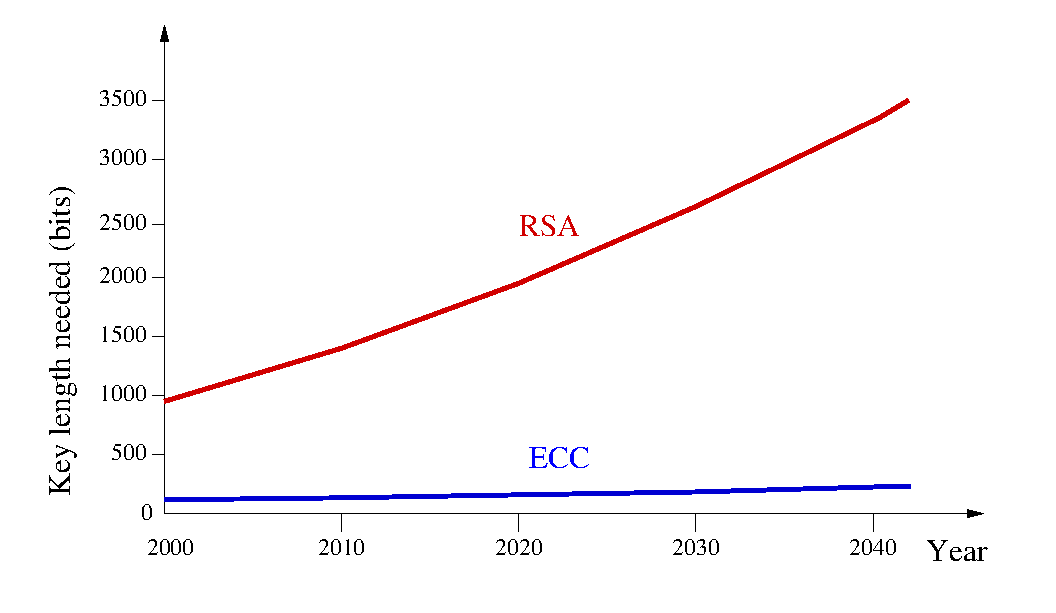
\includegraphics[scale=0.7]{figures/RSAKeyLength-2}
\caption{Prognose f�r die Entwicklung der als sicher betrachteten
  Schl�ssell�ngen bei RSA und bei Elliptische Kurven} 
\label{RSAKeylength}
\end{center}
\vskip -30 pt
\end{figure}

\newpage

Bei der digitalen Signatur muss man differenzieren: f�r die {\em
  Erstellung} einer digitalen Signatur ben�tigen auf Elliptischen
Kurven basierende Verfahren im Vergleich zu RSA nur gut ein Zehntel des
Rechenaufwandes (66 zu 515 Ganzzahlmultiplikationen). Siehe hierzu
Abbildung~\ref{ThousandBitMultiplications} (Quelle: J.  Merkle,
Elliptic Curve Cryptography Workshop, 2001). Betrachtet man die f�r eine
{\em Verifikation} durchzuf�hrenden Rechenschritte, dreht sich dieses Bild
jedoch zu Gunsten von RSA um (112 zu 17 Ganzzahlmultiplikationen). Der 
Grund liegt darin, dass es bei Verwendung des RSA m�glich ist, einen sehr 
kurzen Exponent f�r den �ffentlichen Schl�ssel zu w�hlen, solange der 
private Exponent nur hinreichend lang ist.

% -> Figure 2
\begin{figure}[ht]
\vskip -40 pt
\begin{center}
\vspace{1.5cm}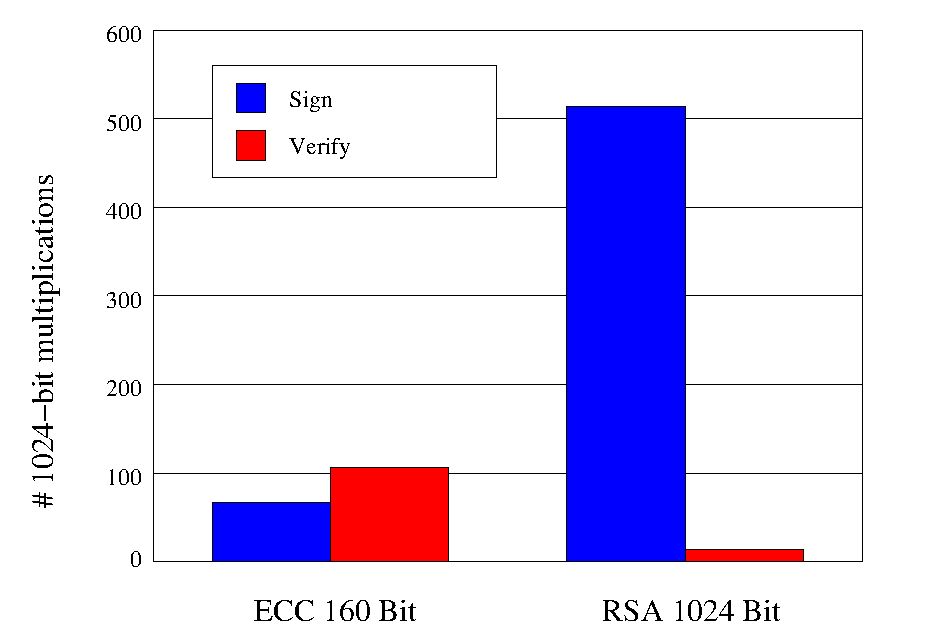
\includegraphics[scale=0.7]{figures/ECCRSA}
\caption{Gegen�berstellung des Aufwands der Operationen Signieren und
         Verifizieren bei RSA und bei Elliptischen Kurven} 
\label{ThousandBitMultiplications}
\end{center}
\vskip -10 pt
\end{figure}

Da bei Smartcards, die auf RSA basieren, stets der lange (private)
Schl�ssel auf der Karte gespeichert werden muss und die Erstellung
der digitalen Signatur, nicht aber die Verifikation, auf der Karte
stattfindet, treten hier deutlich die Vorteile Elliptischer Kurven zutage. 
\par
\smallskip
Das gr��te Problem bei der Implementierung von Verfahren, die auf Elliptischen Kurven beruhen, ist bislang die
mangelnde {\em Standardisierung\index{Standardisierung}}. Es gibt nur eine RSA-Implementierung, aber viele Arten, Elliptische Kurven einzusetzen.
So k�nnen verschiedene Zahlk�rper zugrunde gelegt, eine Vielzahl von (Elliptischen) Kurven --- durch
Parameter beschrieben\footnote{%
Siehe Kapitel \ref{ECC-Crypto}
} --- eingesetzt und unterschiedliche Darstellungen der Kurvenpunkte verwendet werden.
Jede Wahl hat ihre Vorz�ge, so dass f�r jede Anwendung eine andere Implementierung optimal sein kann. Dies
hat jedoch zur Konsequenz, dass Systeme, die auf Elliptischen Kurven beruhen, oftmals nicht interoperabel
sind. Um mit einer beliebigen auf Elliptischen Kurven basierenden Anwendung kommunizieren zu k�nnen, m�sste man
eine Vielzahl von Implementierungen vorhalten, was den Effizienzvorteil gegen�ber der Verwendung von RSA
zunichte macht.

Deshalb bem�hen sich internationale Organisationen um Standardisierung:
IEEE (P1363), ASC (ANSI X9.62, X9.63), ISO/IEC sowie 
RSA Laboratories\index{RSA Laboratories} und Certicom\index{Certicom}. 
Im Gegensatz zur IEEE, die bisher nur eine Beschreibung der verschiedenen
Implementierungen vorgenommen hat, hat die ASC konkret 10 Kurven ausgew�hlt
und empfiehlt deren Verwendung. Der Vorteil des ASC-Ansatzes ist,
dass ein einziges Byte ausreicht, um die verwendete Kurve zu spezifizieren.
Zur Zeit ist jedoch nicht absehbar, ob es der ASC gelingen wird, einen
de-facto-Standard durchzusetzen.

Obwohl aktuell kein Handlungsbedarf besteht\footnote{%
  Aktuelle Informationen zur Sicherheit des RSA-Verfahrens finden Sie in 
  den Kapiteln \ref{SecurityRSA} und \ref{Chapter_Dlog-FactoringDead}.
},
laufende RSA-Anwendungen umzustellen, sollte man ernsthaft den Einsatz
von Elliptischen Kurven erw�gen\footnote{%
  Siehe bspw. die Technische Richtlinie des BSI \glqq Kryptographische Verfahren:
  Empfehlungen und Schl�ssell�ngen\grqq~vom 15. Februar 2016.
}.
Neuere Diskussionen zur Sicherheit von ECC finden Sie in Kapitel
\ref{Chapter_Dlog-FactoringDead}.


% -----------------------------------------------------------------------------
\section{Elliptische Kurven -- Historisches}

Auf dem Gebiet der Elliptischen Kurven wird seit �ber 100 Jahren geforscht. Im Laufe der Zeit hat man
viele weitl�ufige und mathematisch tiefgr�ndige Resultate im Zusammenhang mit Elliptischen Kurven gefunden
und ver�ffentlicht. Ein Mathematiker w�rde sagen, dass die Elliptischen Kurven
(bzw.\ die dahinterstehende Mathematik) gut verstanden sind. Urspr�nglich war diese Forschung reine
Mathematik, das hei�t Elliptische Kurven wurden zum Beispiel in den mathematischen Teilgebieten
Zahlentheorie und algebraische Geometrie untersucht, die allgemein sehr abstrakt sind. Auch in der
nahen Vergangenheit spielten Elliptische Kurven eine bedeutende Rolle in der reinen Mathematik. In den
Jahren 1993 und 1994\footnote%
{
  1994 wurden die Beweisl�cken durch Wiles und Richard Taylor geschlossen.
}
ver�ffentlichte Andrew Wiles\index{Wiles, Andrew} mathematische Arbeiten, die weit �ber das Fachpublikum
hinaus auf gro�e Begeisterung gesto�en sind. In diesen Arbeiten bewies er die Richtigkeit einer --- in
den sechziger Jahren des 20. Jahrhunderts von zwei Japanern aufgestellten --- Vermutung. Dabei geht es
kurz und grob gesagt um den Zusammenhang zwischen Elliptischen Kurven und sogenannten Modulformen.
Das f�r die meisten eigentlich Interessante daran ist, dass Wiles mit seinen Arbeiten auch den ber�hmten
zweiten Satz von Fermat\index{Fermat!letzter Satz} bewiesen hat. Dieser Satz hatte sich seit Jahrhunderten
(Fermat\index{Fermat, Pierre} lebte von 1601 bis 1665) einem umfassenden Beweis durch die Mathematik
entzogen. Dementsprechend
gro� war die Resonanz auf den Beweis durch Wiles. In der Formulierung von Fermat lautet der nach ihm
benannte Satz so (Fermat hat folgende Worte an den Rand des 1621 von Bachet de Meziriac
herausgegebenen Werks von Diophant geschrieben):

\begin{quote} {\em
Cubum autem in duos cubos, aut quadratoquadratum in duos quadratoquadratos, et
generaliter nullam in infinitum ultra quadratum potestatem in duos ejusdem nominis
fas est dividere: cujus rei demonstrationem mirabilem sane detexi. Hanc marginis
exiguitas non caperet.
} \end{quote}

Frei �bersetzt und mit der Schreibweise der heutigen Mathematik bedeutet dies:\\
Es gibt keine positiven ganzen Zahlen $x, y$ und $z$ gr��er als Null, so dass
$x^n + y^n = z^n$ f�r $n>2$ gilt.
Ich habe einen bemerkenswerten Beweis f�r diese Tatsache gefunden, aber es ist
nicht genug Platz am Rand [des Buches], um ihn niederzuschreiben.

Dies ist schon bemerkenswert: Eine relativ einfach zu verstehende Aussage
(gemeint ist Fermats zweiter Satz) konnte erst nach so langer Zeit bewiesen werden, obwohl
Fermat selber angab, schon einen Beweis gefunden zu haben.
Im �brigen ist der Beweis von Wiles sehr umfangreich (alle im Zusammenhang mit dem Beweis
stehenden Ver�ffentlichungen von Wiles ergeben schon ein eigenes Buch). Man sollte sich daher
im klaren sein, dass die Elliptischen Kurven im allgemeinen sehr tiefgreifende Mathematik ber�hren.

Soweit zur Rolle der Elliptischen Kurven in der reinen Mathematik.
Im Jahr 1985 haben Neal Koblitz\index{Koblitz, Neal} und Victor Miller
\index{Miller, Victor} unabh�ngig voneinander vorgeschlagen, 
Elliptische Kurven in der Kryptographie einzusetzen. Damit haben die 
Elliptischen Kurven auch eine ganz konkrete praktische Anwendung gefunden.
Ein weiteres interessantes Einsatzgebiet f�r Elliptische Kurven ist die
Faktorisierung von ganzen Zahlen \index{Faktorisierung}
(auf der \index{Komplexit�t} Schwierigkeit/Komplexit�t, die Primfaktoren
einer sehr gro�en Zahl zu finden, beruht das RSA-Kryptosystem: 
vergleiche Kapitel \ref{SecurityRSA}
). 
In diesem Bereich werden seit 1987 Verfahren untersucht und eingesetzt,
die auf Elliptischen Kurven basieren
(vergleiche Kapitel \ref{ECC-Factorisation}).\\
Es gibt auch Primzahltests\index{Primzahltest}, die auf Elliptischen 
Kurven basieren.
% (s. Anmerkung U. Kuehn)

Elliptische Kurven werden in den verschiedenen Gebieten unterschiedlich
eingesetzt: 
Verschl�sselungsverfahren auf Basis von Elliptischen Kurven beruhen auf der
Schwierigkeit des als Elliptische Kurven Diskreter Logarithmus bekannten 
Problems.
Zur Faktorisierung ganzer Zahlen wird die Tatsache benutzt, dass man eine
gro�e Zahl elliptischer Kurven f�r eine nat�rliche zusammengesetzte Zahl $n$
erzeugen kann.



% -----------------------------------------------------------------------------
\section{Elliptische Kurven -- Mathematische Grundlagen}

In diesem Abschnitt erhalten Sie Informationen �ber
\index{Gruppe} {\em Gruppen} und \index{K�rper} {\em K�rper}.\footnote{%
  Eine didaktisch sehr sch�ne Einf�hrung in Elliptische Kurven finden Sie
  in \cite{Schulz2015}.\index{RSA \& Co. in der Schule}
}


% -----------------------------------------------------------------------------
\subsection{Gruppen}

Da der Begriff der {\em Gruppe} umgangssprachlich anders als in der Mathematik eingesetzt wird, soll der
Vollst�ndigkeit halber an dieser Stelle die wesentliche Aussage der formalen Definition einer Gruppe
kurz eingef�hrt werden:
\begin{itemize}
   \item Eine Gruppe ist eine nichtleere Menge $G$ mit einer Verkn�pfung \glqq $\cdot$\grqq. Die Menge $G$ ist unter der
         Verkn�pfung $\cdot $ abgeschlossen, d.h, sind $a,b$ Elemente aus $G$, so ist auch ihre Verkn�pfung $ab=a\cdot  b$ ein Element aus $G$.
   \item F�r alle Elemente $a, b$ und $c$ aus $G$ gilt: $(ab)c = a(bc)$ (Assoziativgesetz).
   \item Es gibt ein Element $e$ in $G$, das sich bez�glich der Verkn�pfung $\cdot$ neutral verh�lt, d.h., f�r alle $a$ aus der Menge $G:$ gilt $ae = ea = a$.
   \item Zu jedem Element $a$ aus $G$ gibt es ein {\it inverses Element}%
\footnote{Das inverse Element ist eindeutig bestimmt, denn sind $x,y\in G$ zwei Inverse zu $a$, d.h. gilt $ax=xa=e$ und $ay=ya=e$, so folgt $x=xe=x(ay)=(xa)y=ey=y$.}
$a^{-1}$(in $G$), so dass gilt: $aa^{-1} = a^{-1}a = e$.
\end{itemize}

Gilt zus�tzlich noch $ab = ba$ (Kommutativgesetz) f�r alle $a, b$ aus $G$, so nennt
man die Gruppe $G$ eine {\em abelsche} Gruppe.

Da man auf der selben Menge mehrere Verkn�pfung erkl�ren kann, unterscheidet man
diese durch verschiedene Namensgebungen und Zeichen (z.B. $+$ Addition oder $\cdot$
Multiplikation). 

Als einfachstes Beispiel einer (abelschen) Gruppe sei die Gruppe der ganzen Zahlen
mit der �blichen Addition genannt. Die Menge der ganzen Zahlen wird mit ${\mathbb Z}$
bezeichnet. ${\mathbb Z}$ hat unendlich viele Elemente:
${\mathbb Z} = \{ \cdots, -4, -3, -2, -1, 0, 1, 2, 3, 4, \cdots\}$.
Die Verkn�pfung von zum Beispiel $1+2$ liegt in ${\mathbb Z}$, denn $1+2 = 3$ und $3$
liegt in ${\mathbb Z}$. Das neutrale Element der Gruppe ${\mathbb Z}$ ist $0$.
Das inverse Element von $3$ ist $-3$, denn $3+(-3) = 0$.

F�r unsere Zwecke besonders interessant sind sogenannte {\em endliche} Gruppen.
D.h. es gibt die zugrundeliegende Menge $\mathcal{M}$ mit einer endlichen Anzahl von
Elementen und die Operation $+$, so dass die obigen Bedingungen erf�llt sind.
Beispiele sind die Gruppen ${\mathbb Z}_n = \{0, 1, 2, 3, \cdots, n-1\}$ der Teilerreste
bei der Division durch $n \in {\mathbb N}$, mit der Addition mod $n$ als Verkn�pfung.

\paragraph*{Zyklische Gruppen}\index{Gruppe!zyklisch}
Als {\it zyklische Gruppen}\footnote{Zyklische Gruppen k�nnen grunds�tzlich auch unendlich sein wie z.B. die additive Gruppe der ganzen Zahlen. Wir betrachten hier jedoch nur endliche zyklische Gruppen.} bezeichnet man solche Gruppen $G'$, die ein Element $g$ besitzen, aus dem man
mittels der Gruppen-Verkn�pfung alle anderen Elemente der Gruppe erzeugen kann. Es gibt also f�r jedes
Element $a$ aus $G'$ eine positive, ganze Zahl $i$, so dass die $i$-fache Verkn�pfung von $g$ mit sich
selbst $g^i = g\cdot g \cdots g = a$. Das Element $g$ ist ein {\em Generator} der zyklischen Gruppe --- jedes Element
in $G'$ l�sst sich mittels $g$ und der Verkn�pfung erzeugen.


\paragraph*{Ordnung von Elementen einer Gruppe}\index{Gruppe!Ordnung}
Nun zur Ordnung eines Elements der Gruppe: Sei $a$ aus $G$. Die kleinste positive ganze Zahl $r$ f�r
die gilt, dass $a^r$, also $r$ mal $a$ mit sich selbst verkn�pft, das neutrale Element der Gruppe $G'$ ist
(d.h. $a^r = e$), nennt man {\em Ordnung} von $a$.

Die {\it Ordnung der Gruppe} ist die Anzahl der Elemente in der Menge $G$. Ist die Gruppe $G$ zyklisch und $g$ ein Generator, so stimmt die Ordnung von $g$ mit der Gruppenordnung �berein. Man kann leicht zeigen, dass die Ordnung eines Gruppenelements stets die Gruppenordnung teilt. Hieraus folgt insbesondere, dass Gruppen mit Primzahlordnung (d.h. die Ordnung der Gruppe ist eine Primzahl) zyklisch sind.


% -----------------------------------------------------------------------------
\subsection{K�rper}

In praktischen Anwendungen betrachtet man h�ufig Mengen, auf denen nicht nur eine (Grup"-pen"~)
Verkn�pfung, sondern zwei Verkn�pfungen definiert sind. Diese nennt man oft Addition und Multiplikation. Die mathematisch interessantesten Mengen dieser Art sind sogenannte K�rper, wie z.B. die Menge der reellen Zahlen.

Unter einem K�rper versteht man in der Mathematik eine Menge $K$ mit den zwei Verkn�p"-fungen Addition und Multiplikation (mit $+$ und $\cdot$ bezeichnet), so dass die folgenden Bedingungen erf�llt sind:
\begin{itemize}
   \item Die Menge $K$ ist zusammen mit der Verkn�pfung $+$ (Addition) 
         eine abelsche Gruppe. Dabei sei $0$ das neutrale Element der 
	 Verkn�pfung $+$.
   \item Die Menge $K\setminus\{0\}$ (d.h. $K$ ohne das Element 0) ist 
         zusammen mit der Verkn�pfung $\cdot$ (Multiplikation)
         ebenfalls eine abelsche Gruppe. Dabei sei $1$ das neutrale Element
	 der Verkn�pfung $\cdot$.
   \item F�r alle Elemente $a, b$ und $c$ aus $K$ gilt
         $c\cdot (a+b) = c \cdot a + c \cdot b$ und
         $(a+b) \cdot c = a \cdot c + b \cdot c$ (Distributivgesetz).
\end{itemize}

K�rper k�nnen endlich viele oder unendliche viele Elemente enthalten --- je nachdem nennt man den K�rper {\em endlich} oder {\em unendlich}. So sind die uns vertrauten K�rper der rationalen bzw. der reellen Zahlen unendlich. Beispiele f�r endliche K�rper sind die Primk�rper
${\mathbb Z}_p = \{0, 1, 2, 3, \cdots, p-1\}$, $p$ eine Primzahl, versehen mit
der Addition modulo $p$ und der Multiplikation modulo $p$ (auch Restklassenk�rper genannt).
\index{K�rper!Charakteristik}
\paragraph*{Charakteristik eines K�rpers}
Die Charakteristik eines K�rper $K$ ist die Ordnung des neutralen Elements der Multiplikation ($1$-Element) bez�glich der Addition, d.h. die kleinste nat�rliche Zahl $n$, so dass gilt
$$ \underbrace{1 + 1 + \cdots + 1}_{\hbox{$n$ mal}} =0
 \, ,
$$
wobei $0$ das neutrale Element der Addition ist.
Gibt es keine solche nat�rliche Zahl, d.h. ergibt $1 + 1 + \cdots + 1$ unabh�ngig von der Zahl der Summanden nie das neutrale Element der Addition $0$, so sagt man, der K�rper habe Charakteristik $0$.

K�rper mit Charakteristik $0$ haben daher stets die (paarweise verschiedenen) Elemente $1, 1+1, 1+1+1, \dots$ und sind folglich stets unendlich; andererseits k�nnen K�rper mit endlicher Charakteristik durchaus endlich oder auch unendlich sein.
Ist die Charakteristik $n$ endlich, so muss sie eine Primzahl sein, denn w�re sie zusammengesetzt, d.h. $n=pq$, so sind $p,q<n$ und aufgrund der Minimalit�t der Charakteristik ist keines der K�rperelemente $\bar p=\underbrace{1 + 1 + \cdots + 1}_{\hbox{$p$ mal}}$, $\bar q=\underbrace{1 + 1 + \cdots + 1}_{\hbox{$q$ mal}}$ gleich $0$. Folglich existieren Inverse $\bar p^{-1},\bar q^{-1}$ bez�glich der Multiplikation. Dann ist aber $(\bar p\bar q)( \bar p^{-1}\bar q^{-1})=1$, andererseits ist nach Definition der Charakteristik $\bar p\bar q=\bar n=\underbrace{1+1+\dots+1}_{\hbox{$n$ times}}=0$ und somit $\underbrace{(\bar p\bar q)}_{=0}( \bar p^{-1}\bar q^{-1})=0$, was zu einem Widerspruch f�hrt.

\begin{example}{:} Der K�rper ${\mathbb Z}_p$, $p$ prim, hat die Charakteristik $p$. Ist $p$ nicht prim, so ist ${\mathbb Z}_p$ gar kein K�rper.
\end{example}

Der einfachste, denkbare K�rper ist ${\mathbb Z}_2 \; = \{ 0,1\}$, der nur Null- und Einselement enth�lt. Dabei ist $0+0=0$, $0+1=1+0=1$, $1+1=0$, $1\cdot 1=1$, $0\cdot 0=0\cdot 1=1\cdot 0=0$.

\index{K�rper!endlich}
\paragraph*{Endliche K�rper}
Wie bereits erw�hnt, hat jeder endliche K�rper eine Charakteristik $p\ne 0$, wobei $p$ eine Primzahl ist. Zu jeder Primzahl $p$ gibt es einen K�rper mit $p$ Elementen, n�mlich ${\mathbb Z}_p$.

Die Anzahl der Elemente eines K�rpers muss jedoch im allgemeinen keine Primzahl sein. So ist es nicht schwer, einen K�rper mit $4$ Elementen zu konstruieren\footnote{%
Die Menge $K=\{0,1,a,b\}$ ist mit den Verkn�pfungen der folgenden Tabellen ein K�rper:\\
$
\begin{array}{|c||c|c|c|c|} 
\hline 
+ & 0 & 1 & a & b\\
\hline \hline
0 & 0 & 1 & a & b\\
\hline 
1 & 1 & 0 & b & a\\
\hline 
a & a & b & 0 & 1\\
\hline 
b & b & a & 1 & 0\\
\hline 
\end{array} \qquad {\rm ~und~} \qquad
\begin{array}{|c||c|c|c|c|} 
\hline 
\cdot & 0 & 1 & a & b\\
\hline \hline
0 & 0 & 0 & 0 & 0\\ 
\hline 
1 & 0 & 1 & a & b\\ 
\hline 
a & 0 & a & b & 1\\ 
\hline 
b & 0 & b & 1 & a\\
\hline 
\end{array} 
$\\
}.

Man kann zeigen, dass die Ordnung jedes K�rpers eine Primzahlpotenz (d.h. die Potenz einer Primzahl) ist. Andererseits kann man zu jeder Primzahlpotenz $p^n$ einen K�rper konstruieren, der die Ordnung $p^n$~hat. Da zwei endliche K�rper mit gleicher Zahl von Elementen nicht unterscheidbar\footnote{Sind $K,K'$ zwei K�rper mit $k=p^n$ Elementen, so gibt es eine eineindeutige Abbildung $\varphi:K\to K'$, die sich mit der K�rperarithmetik vertr�gt. Eine solche Abbildung nennt man Isomorphie. Isomorphe K�rper verhalten sich mathematisch gleich, so dass es keinen Sinn macht, zwischen ihnen zu unterscheiden. Z.B. sind ${\mathbb Z}_2$ und $K'=\{ NULL,EINS\}$ mit Nullelement $NULL$ und Einselement $EINS$ isomorph. Hierbei sei darauf hingewiesen, dass mathematische Objekte ausschlie�lich �ber ihre Eigenschaften definiert sind.} sind, spricht man von {\bf dem\ K�rper mit $p^n$ Elementen} und bezeichnet diesen mit $GF(p^n)$ oder im Amerikanischen mit
$\mathbb{F}_p^{n}$. Dabei steht $GF$ f�r {\it Galois Feld} in Erinnerung an den franz�sischen Mathematiker Galois.

Eine besondere Rolle spielen die K�rper $GF(p)$, deren Ordnung eine Primzahl ist. Man
nennt solche K�rper Primk�rper zur Primzahl $p$ und bezeichnet ihn meist ebenfalls
mit ${\mathbb Z}_p$.\footnote{%
  F�r Primk�rper sind die additive Gruppe sowie die multiplikative Gruppe zyklisch.
  Ferner enth�lt jeder K�rper $GF(p^n)$ einen zu ${\mathbb Z}_p$ isomorphen Primk�rper.
}


% -----------------------------------------------------------------------------
\section{Elliptische Kurven in der Kryptographie} \label{ECC-Crypto}

In der Kryptographie sind elliptische Kurven ein n�tzliches Werkzeug. Solche Kurven
ergeben sich als L�sung"-en einer Gleichung der Form\footnote{%
  Die hier verwendete Kurve erh�lt man als Nullstellen des {\it Polynoms}\index{Polynom}
  $F$ vom Grad drei in drei Variablen. Dabei bezeichnet man allgemein Ausdr�cke der Form
  % yyyyyyyccc    $P=\sum_{i_1,\dots,i_n\in\N_0} a_{i_1\dots i_n} x_1^{i_1}\dots x_n^{i_n}$
  % yyyyyyyccc yyyyyyyyyyyycccc 3.8.: Erst nach Einf�hren von \begin{bibunit}
  % meldete er hier (in D und E) bei N_0 zurecht: Undefined control sequence.
  $P=\sum_{i_1,\dots,i_n\in\mathbb{N}} a_{i_1\dots i_n} x_1^{i_1}\dots x_n^{i_n}$
  mit Koeffizienten $a_{i_1\dots i_n}\in K$ als Polynome in $n$ Variablen $x_1,\dots,x_n$
  �ber dem K�rper $K$, wenn ${\rm grad\,} P:=\max\{i_1+\dots +i_n: a_{i_1\dots i_n}\ne 0\}$
  einen endlichen Wert hat, die Summe also nur aus endlich vielen Summanden (Monomen) besteht.
  Die Summe der Exponenten der Variablen jedes einzelnen Summanden ist maximal $3$,
  bei mindestens einem Summanden kommt $3$ als Exponentwert einer Variablen auch wirklich vor.
}

\begin{equation}
 F(x_1,x_2,x_3)=-x_1^3+x_2^2x_3+a_1x_1x_2x_3-a_2x_1^2x_3+a_3x_2x_3^2-a_4x_1x_3^2-a_6x_3^3=0.
\label{eccbasisgleichung}
\end{equation}

Dabei sind die Variablen $x_1,x_2,x_3$ sowie die Parameter $a_1,\dots,a_4,a_6$ Elemente eines gegebenen K�r"pers $K$. K�rper und Parameter m�ssen so gew�hlt werden, dass die Kurve bestimmte, f�r die Kryptographie relevante Eigenschaften besitzt. Der zugrunde liegende K�rper $K$ kann einfach die bekannte Menge der reellen Zahlen oder auch ein endlicher K�rper sein (vgl. letzter Abschnitt).
Damit sich eine sinnvolle Kurve ergibt, m�ssen die Parameter so gew�hlt sein, dass die folgenden Nebenbedingungen gelten
$$ \frac{\partial F}{\partial x_1}\ne 0, \quad \frac{\partial F}{\partial x_2}\ne 0, \quad
\frac{\partial F}{\partial x_3}\ne 0 .
$$
Ferner betrachten wir Punkte, die sich nur durch eine Vervielfachung jeder Komponente ergeben, als identisch, denn mit $(x_1,x_2,x_3)$ erf�llt stets auch $\alpha (x_1,x_2,x_3)$ ($\alpha\ne 0$) die Ausgangsgleichung. Formal betrachten wir daher �quivalenzklassen von Punkten $(x_1,x_2,x_3)$, wobei wir zwei Punkte als gleich ansehen, wenn sie durch Multiplikation mit einer skalaren Konstante $\alpha \ne 0$ auseinander hervorgehen.
\\ Setzt man in der Ausgangsgleichung $x_3=0$, so wird diese zu $-x_1^3=0$, also $x_1=0$. Folglich ist die �quivalenzklasse, die das Element $(0,1,0)$ enth�lt, die einzige Punkt mit $x_3=0$. F�r alle anderen L�sungspunkte k�nnen wir die Transformation
$$ K\times K\times (K\setminus\{0\})\ni (x_1,x_2,x_3) \mapsto (x,y):=\left( \frac{x_1}{x_3}, \frac{x_2}{x_3}\right) \in K\times K
$$
vornehmen, die die Anzahl der Variablen von drei auf zwei reduziert. 
Die Ausgangsgleichung $F(x_1,x_2,x_3)=0$ war so gew�hlt, dass sich auf
diese Weise die sogenannte Weierstrass-Glei"-chung\footnote{%
Karl Weierstrass\index{Weierstrass, Karl}, 31.10.1815$-$19.12.1897, deutscher Mathematiker, 
Verfechter der streng formalen Ausrichtung der Mathematik.
}
\begin{equation}
 y^2+a_1xy+a_3y = x^3+a_2x^2+a_4x+a_6
\label{ell}
\end{equation}
ergibt.
Da alle bis auf einen L�sungspunkt durch die Gleichung (\ref{ell}) beschrieben werden k�nnen, bezeichnet man (\ref{ell}) auch oft als die Elliptische Gleichung, ihre L�sungsmenge folglich mit
$$ {\bf E} = \left\{(x,y)\in K\times K \, |\, y^2+a_1xy+a_3y = x^3+a_2x^2+a_4x+a_6  \right\} \cup \{{\cal O} \}.
$$
Dabei soll ${\cal O}$ den auf diese Weise nicht beschriebenen Punkt $(0,1,0)$ darstellen, der durch die Projektion (Division durch $x_3$) quasi in den unendlich fernen Punkt abgebildet wird.

% -> Figure 3
\begin{figure}[ht]
\begin{center}
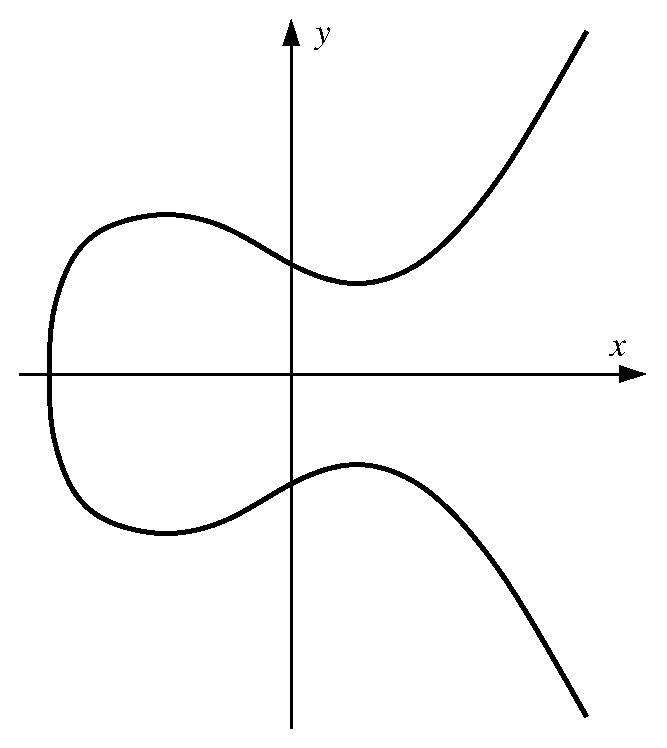
\includegraphics[scale=0.60]{figures/elliptic-curve}
\caption{Beispiel einer Elliptischen Kurve �ber dem K�rper der reellen Zahlen} 
\label{ExampleEllipticCurve}
\end{center}
\vskip -10 pt
\end{figure}
Als zugrunde liegenden K�rper f�r eine Elliptische Kurve verwendet man in der Kryptographie stets endliche K�rper $K=GF(p^n)$, also nicht wie in Abbildung \ref{ExampleEllipticCurve} die zu einer stetigen Kurve f�hrenden reellen Zahlen. Der Grund liegt, einfach gesagt, darin, dass wir bei der Verarbeitung und �bertragung von Nachrichten stets nur endlich viele Zust�nde zur Verf�gung haben (aufgrund der Arbeitsweise moderner Computer), K�rper mit unendlich vielen Elementen wie z.B. die reellen Zahlen daher stets nur unvollst�ndig darstellen k�nnen.

In der Praxis hat es sich als sinnvoll erwiesen, entweder $GF(p)$ mit einer gro�en Primzahl $p$ oder $GF(2^n)$ mit einer (gro�en) nat�rlichen Zahl $n$ zu betrachten. Der Grund f�r die Verwendung des Primk�rpers $GF(p)$ liegt in seiner einfachen Arithmetik; andererseits kommt $GF(2^n)$ der bin�ren Darstellung in Computersystemen entgegen. Andere K�rper wie z.B. $GF(7^n)$ bieten keiner dieser beiden Vorteile und werden daher in der Praxis nicht verwendet, ohne dass dies theoretische Gr�nde h�tte.

Durch Koordinatentransformation kann man die Weierstrass-Gleichung\index{Weierstrass, Karl} in einer einfacheren Form schreiben\footnote{Anschaulich bedeutet eine solche Koordinatentransformation eine Drehung bzw. Streckung der Koordinatenachsen, ohne dass die zugrunde liegende Kurve selbst ver�ndert wird.}.  Je nachdem, ob $p>3$ ist, verwendet man unterschiedliche Transformationen und erh�lt so

\begin{itemize}
\item im Fall $GF(p)$, $p>3$, die Elliptische Kurven-Gleichung der Form
\begin{equation}
 y^2 = x^3 + ax + b
\label{ellp}
\end{equation}
mit $4a^3+27b^2\ne 0$
\item im Fall $GF(2^n)$ die Elliptische Kurven-Gleichung der Form
\begin{equation}
 y^2+xy = x^3 + ax^2 + b
\label{ell2}
\end{equation}
mit $b\ne 0$\footnote{Die Form (\ref{ellp}) ist die Standardform der Weierstrass-Gleichung\index{Weierstrass, Karl}. Ist die Charakteristik des K�rpers jedoch $2$ oder $3$, so ist $4=0$ bzw. $27=0$, was dazu f�hrt, dass man in der Bedingung an die Parameter $a,b$ wesentliche Informationen verliert. Dies ist ein Hinweis darauf, dass die Transformation auf die Standardform in diesen F�llen nicht zu befriedigenden Ergebnissen f�hrt.}.
\end{itemize}
Durch diese Bedingungen an die Parameter $a,b$ ist gew�hrleistet, dass die Elliptische Gleichung f�r kryptographische Anwendungen geeignet ist\footnote{Formal sagt man, die Kurve ist nicht singul�r.}.


F�r die Anzahl $|E|$ der Elemente einer Elliptischen Kurve $E$ �ber einem K�rper $GF(k)$ (praktisch $k=p$ prim oder $k=2^n$) gilt nach dem Satz von Hasse \cite{Silverman2009} die einfache Beziehung $| \, |E| - k-1\,| \le 2\cdot \sqrt{k}$. Diese Ungleichung ist �quivalent zu $k+1 - 2\sqrt{k} < |E| < k+1+2\sqrt{k}$. Dies bedeutet, dass die Anzahl der Elemente der Elliptischen Kurve mit der Gr��e $k$ gut abgesch�tzt werden kann. 

% $$ (\sqrt{k}-1)^2=k-2\sqrt{k}+1 \le |E| \le k+1 .
% $$
% Dies bedeutet, dass f�r gro�e $k$ die Anzahl der Elemente der Elliptischen Kurve praktisch wie $k$ w�chst.


% -----------------------------------------------------------------------------
\section{Verkn�pfung auf Elliptischen Kurven}

Um mit Elliptischen Kurven arbeiten zu k�nnen, definiert man eine Verkn�pfung (meist additiv als $+$ geschrieben) auf den Punkten der Elliptischen Kurve. Dabei definiert man bei Elliptischen Kurven �ber $GF(p)$ die kommutative Verkn�pfung durch
\begin{enumerate}
\item $P+{\cal O}={\cal O}+P=P$ f�r alle $P\in E$,
\item f�r $P=(x,y)$ und $Q=(x,-y)$ ist $P+Q={\cal O}$,
\item f�r $P_1=(x_1,x_2),P_2=(x_2,y_2)\in E$ mit $P_1,P_2\ne {\cal O}$ und $(x_2,y_2)\ne (x_1,-y_1)$ ist $P_3:=P_1+P_2$, $P_3=(x_3,y_3)$ definiert durch
$$ x_3:=-x_1-x_2+\lambda^2 \, , \qquad y_3:=-y_1+\lambda (x_1-x_3)
$$
mit dem Hilfsquotienten
$$ \lambda:=\left\{ \begin{array}{cl} \frac{y_1-y_2}{x_1-x_2} & {\rm falls~} P_1\ne P_2,\\
                                     \frac{3x_1^2+a}{2y_1} & {\rm falls~} P_1=P_2. \end{array} \right.
$$
\end{enumerate}
Hieraus folgt insbesondere f�r $P=(x,y)\in E$, dass gilt $-P=(x,-y)$.

�ber $GF(2^n)$ definiert man analog die Verkn�pfung durch
\begin{enumerate}
\item $P+{\cal O}={\cal O}+P=P$ f�r alle $P\in E$,
\item f�r $P=(x,y)$ und $Q=(x,x+y)$ ist $P+Q={\cal O}$,
\item f�r $P_1=(x_1,x_2),P_2=(x_2,y_2)\in E$ mit $P_1,P_2\ne {\cal O}$ und $(x_2,y_2)\ne (x_1,x_1+y_1)$ ist $P_3:=P_1+P_2$, $P_3=(x_3,y_3)$ definiert durch
$$ x_3:=-x_1+x_2+\lambda+\lambda^2+a \, , \qquad y_3:=y_1+x_3+\lambda (x_1+x_3)
$$
mit
$$ \lambda:=\left\{ \begin{array}{cl} \frac{y_1+y_2}{x_1+x_2} & {\rm falls~} P_1\ne P_2,\\
                                   x_1+\frac{y_1}{x_1} & {\rm falls~} P_1=P_2. \end{array}\right.
$$
\end{enumerate}
Hieraus folgt insbesondere f�r $P=(x,y)\in E$, dass gilt $-P=(x,x+y)$.

(Beachte: $-(-P)=(x,x+(x+y))=(x,2x+y)=(x,y)$, da der zugrunde liegende K�rper Charakteristik $2$ hat.)\footnote{%
Eine Animation der Punktaddition auf Elliptischen Kurven 
findet man auf der Certicom-Seite\index{Certicom} unter\\
\url{https://www.certicom.com/ecc-tutorial} (Datum letzte �nderung unklar).\\
Vergleiche auch den Web-Link zum \hyperlink{ec:Web-Link:Java_Laubrock}
{Java-Tutorial} am Ende dieser Kapitels.

}

Man kann nachrechnen, dass die Menge $E\cap\{\cal O\}$ mit der so definierten
Addition eine Gruppe bildet. Dies bedeutet insbesondere, dass die Summe zweier
Kurvenpunkte stets wieder ein Punkt auf der Elliptische Kurve ist. Diese
Addition l��t sich auch geometrisch veranschaulichen, wie der folgende
Abschnitt zeigt.

% \newpage
\begin{figure}[htbp]
\subsection*{Addieren von Punkten auf einer Elliptischen Kurve}
Die zwei folgenden Abbildungen zeigen, wie bei einer Elliptischen Kurve �ber den reellen Zahlen in affinen Koordinaten
zwei Punkte addiert werden. Der unendlich ferne Punkt ${\cal O}$ kann nicht in der affinen 
Ebene dargestellt werden.  
\begin{center}
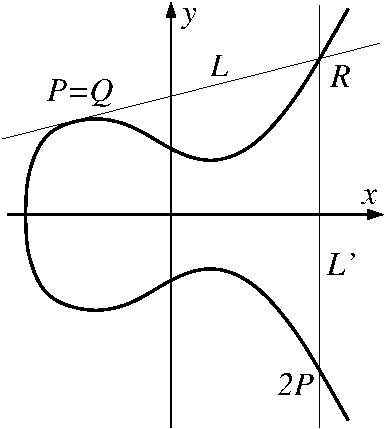
\includegraphics[scale=1.08]{figures/ec-mult2}
\caption{Verdoppelung eines Punktes} 
\vspace{\floatsep}
\vskip +20 pt
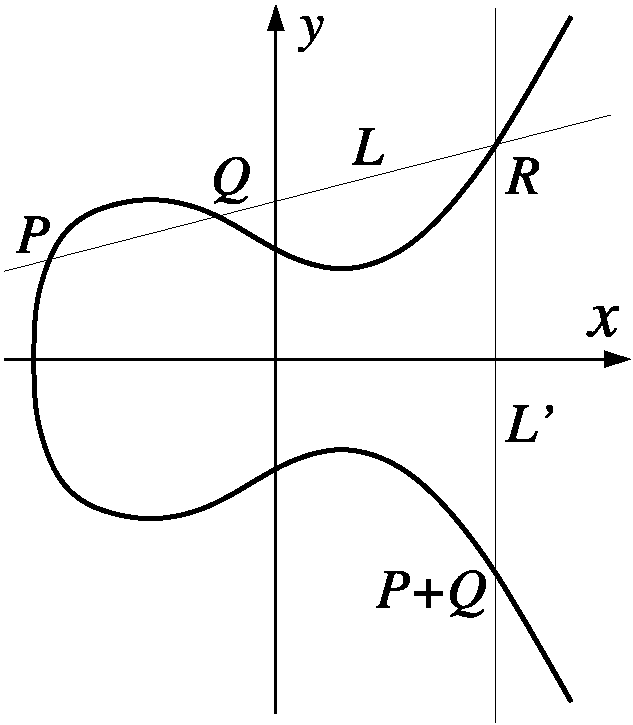
\includegraphics[scale=0.65]{figures/ec-add}  %be_2005 evtl. an diesem Vergr��erungsfaktor spielen
\caption{Addition zweier verschiedener Punkte im K�rper der reellen Zahlen} % \footnotemark }
\end{center}
\end{figure}
% \addtocounter{footnote}{0}\footnotetext{Der Punkt $O$ kann nicht in der affinen Ebene dargestellt werden.}
\enlargethispage{+20pt}
\newpage


% -----------------------------------------------------------------------------
\section[Sicherheit der Elliptischen-Kurven-Kryptographie: Das ECDLP]{\sloppy Sicherheit der Elliptischen-Kurven-Kryptographie: Das ECDLP}

Wie bereits in Abschnitt \ref{ECC-Crypto} erw�hnt, betrachten wir in der Kryptographie Elliptische Kurven �ber diskreten\footnote{Diskret im Gegensatz zu kontinuierlich.} K�rpern $GF(2^n)$ oder $GF(p)$ (f�r gro�e Primzahlen $p$). Dies bedeutet, dass alle Parameter, die zur Beschreibung der Elliptischen Kurve notwendig sind, aus diesem zugrunde liegenden K�rper stammen. Ist nun $E$ eine Elliptische Kurve �ber einem solchen K�rper und $P$ ein Punkt auf der Kurve $E$, so kann man f�r jede nat�rliche Zahl $m$
$$ mP := \underbrace{P+P+\dots+P}_{\hbox{$m$ mal}}
$$
bilden. Diese Operation ist aus kryptographischer Sicht deshalb besonders interessant, weil man einerseits um $mP$ zu berechnen im allgemeinen nur $\log m$ Additionen durchf�hren muss --- man bildet einfach $P$, $2P$, $2^2P$, $2^3P$, \dots, schreibt $m$ bin�r und addiert schlie�lich entsprechend der Bin�rdarstellung von $m$ auf --- es andererseits sehr aufwa"ndig zu sein scheint, zu gegebenen Punkten $P$ und $Q=mP$ auf $E$ die Zahl $m$ zu bestimmen. Nat�rlich kann man die Folge $P,2P,3P,4P,5P,\dots$ bilden und jeweils mit $Q$ vergleichen. Hierzu ben�tigt man jedoch $m$ Additionen.

Bisher ist noch kein Algorithmus bekannt, der effizient $m$ aus $P$ und $Q$ berechnet. Die bisher besten Verfahren liegen z.B. im Fall $GF(p)$ in der Gr��enordnung $\sqrt{q}$, wobei $q$ ein (gro�er) Primfaktor von $p-1$ ist; $m$ selbst sollte in diesem Fall zwischen $1$ und $q$ liegen, so dass man f�r die Muliplikation $mP$ maximal $\log q$ Schritte ben�tigt. Der Quotient $\frac{\sqrt{q}}{\log q}$ strebt jedoch (schnell) gegen $+\infty$.

Sind die Parameter hinreichend gro� (ist zum Beispiel $p$ prim und
mehr als $160$ Bit lang) ist der Computer ohne weiteres in der Lage, sehr schnell (in wenigen
Bruchteilen einer Sekunden) den Punkt $mP$ zu bestimmen. Das {\it inverse Problem}, $m$ aus $mP$ und $P$ zu erhalten, ist jedoch nicht in akzeptabler Zeit m�glich.

Dies wird als das \glqq Diskrete Logarithmus Problem �ber Elliptischen
Kurven\grqq\ bezeichnet (auch ECDLP\index{ECDLP} -- Elliptic Curve Discrete
Logarithm Problem -- abgek�rzt).

\vskip +5 pt

Formal betrachten wir in der Elliptischen-Kurven-Kryptographie die Punkte der Kurve als Elemente einer Gruppe mit der Addition als Verkn�pfung. Allerdings sind nur solche Elliptischen Kurven f�r kryptographische Anwendungen geeignet, bei der die Anzahl der Kurvenpunkte hinreichend gro� ist. Ferner k�nnen in Spezialf�llen Elliptische Kurven auch aus anderen Gr�nden ungeeignet sein. Das bedeutet, dass man bei der
Definition einer Kurve auf die Wahl der Parameter achten muss. Denn f�r bestimmte Klassen von
Elliptischen Kurven ist es m�glich, das ECDLP leichter zu l�sen als im allgemeinen Fall. Kryptographisch
ungeeignete Elliptische Kurven sind die sogenannten {\em anormalen} Kurven (das sind Kurven �ber ${\mathbb Z}_p$,
f�r die die Menge ${\bf E}$ genau $p$ Elemente hat) und die {\em supersingul�ren} Kurven (das sind Kurven, f�r die man das
Berechnen des ECDLP auf das Berechnen des \glqq normalen\grqq\ Diskreten Logarithmus in anderen endlichen K�rper
reduzieren, d.h. vereinfachen, kann). Daher gibt es kryptographisch gute und schlechte Kurven. Allerdings
kann man f�r gegebene Parameter $a$ und $b$ mit etwas Aufwand feststellen, ob die resultierende Elliptische
Kurve kryptographisch brauchbar ist oder nicht. Die in der Kryptographie eingesetzten Kurven werden meist
von Fachleuten zur Verf�gung gestellt. Sie gew�hrleisten, dass die von ihnen als sicher eingestuften
Elliptischen Kurven den aktuellen Sicherheitsanforderungen gen�gen.
\vskip +5 pt

Bei sicheren Kurven wird haupts�chlich
durch den Parameter $p$ im Fall des zugrunde liegenden K�rpers $GF(p)$ bzw. $n$ im Fall des zugrunde liegenden K�rpers $GF(2^n)$ bestimmt, wie lange es dauert, das ECDLP auf dieser Kurve zu l�sen. Je gr��er diese
Parameter sind, desto l�nger nimmt das L�sen des Problems in Anspruch. Von Fachleuten wird z.B. eine Bitl�nge
von �ber $200$ Bit f�r den Parameter $p$ empfohlen. Hier wird deutlich, warum die Elliptischen Kurven so
interessant f�r die Kryptographie sind. Denn die Parameter bestimmen auch den
Signatur-/Verschl�sselungsaufwand, wenn mit Elliptischen Kurven
Kryptographie betrieben wird. Die Dauer einer Schl�sselpaar-Erzeugung ist ebenfalls von den Parametern abh�ngig. Daher sind kleine Werte (wenige Bits) w�nschenswert (m�glichst schnelle Laufzeiten der Verfahren);
allerdings muss die geforderte Sicherheit dabei eingehalten werden.
Mit einer L�nge von zum Beispiel $200$ Bit f�r $p$ ist eine {\em gute} Elliptische Kurve
genau so sicher wie ein \index{RSA!Modulus} RSA-Modulus von �ber $1024$ Bit L�nge
(zumindest nach dem heutigen Forschungstand). Der Grund daf�r ist, dass die schnellsten
Algorithmen zum L�sen des {\em Elliptische Kurven Diskreter Logarithmus}-Problems eine
exponentielle Laufzeit haben --- im Gegensatz zu den subexponentiellen Laufzeiten, die
die zur Zeit besten Faktorisierungsalgorithmen haben (Zahlk�rpersieb, Quadratisches Sieb
oder Faktorisieren mit Elliptischen Kurven). Dies erkl�rt, warum die Parameter von
Kryptoverfahren, die auf dem Problem {\em Faktorisieren von ganzen Zahlen} beruhen,
gr��er sind als die Parameter von Kryptoverfahren, die auf dem ECDL-Problem basieren.


% -----------------------------------------------------------------------------
\section{Verschl�sseln und Signieren mit Hilfe Elliptischer Kurven}

\begin{sloppypar}
  Das {\em Elliptische Kurven Diskreter Logarithmus
    Problem}\index{Logarithmusproblem} (ECDLP) \index{ECDLP} ist die
  Grundlage f�r die Elliptische-Kurven-Kryptographie. Darauf basierend gibt es verschiedene Signaturverfahren. Um ein solches Signaturverfahren anzuwenden, ben�tigt man:
\end{sloppypar}
\begin{itemize}
    \item Eine Elliptische Kurve {\bf E}, beschrieben durch den zugrunde liegenden K�rper $GF(p^n)$.
    \item Eine Primzahl $q\ne p$ sowie einen Punkt $G$ auf der Elliptischen Kurve ${\bf E}$ mit Ordnung $q$. D.h., es gilt $qG={\cal O}$ und $rG\ne {\cal O}$ f�r alle $r\in \{1,2,\dots,q-1\}$. Die Zahl $q$ muss dann ein Teiler der Gruppenordnung (entspricht der Anzahl der Elemente) $\#{\bf E}$ sein. Aufgrund der Primordnung, erzeugt $G$ eine zyklischen Untergruppe von ${\bf E}$ mit Ordnung $q$.
\end{itemize}
Die genannten Parameter bezeichnet man als \index{Domain-Parameter} {\em Domain}-Para\-meter. Durch sie wird
festgelegt, auf welcher Elliptischen Kurve ${\bf E}$ und in welcher zyklischen Untergruppe von ${\bf E}$ ein
Signaturverfahren eingesetzt  wurde.

\par
%\smallskip
%{\bf Verschl�sselung:}
\subsection{Verschl�sselung}

Mit Hilfe Elliptischer Kurven kann ein sicherer Schl�sselaustausch nach dem \hyperlink{DH-KeyExch}{Diffie-Hellman}-Protokoll \index{Diffie-Hellman} erfolgen (siehe Kapitel \ref{DH-KeyExch}). Dieser Schl�ssel kann dann f�r eine anschlie�ende symmetrische Verschl�sselung verwendet werden. Ein Schl�sselpaar mit privatem und �ffentlichem Schl�ssel wird im Gegensatz zum RSA-Algorithmus nicht erzeugt!

In der Schreibweise der Elliptischen Kurven liest sich das Diffie-Hellman Verfahren wie folgt: Zun�chst einigen sich beide Partner (A und B) �ffentlich auf eine Gruppe $G$ und eine ganze Zahl $q$. Danach w�hlen sie zuf�llig $r_A,r_B\in\{1,2,\dots,q-1\}$, bilden die Punkte $R_A=r_AG$, $R_B=r_BG$ auf der Elliptischen Kurve und tauschen diese aus. Danach berechnet A leicht $R=r_AR_B$. Denselben Punkt (n�mlich $r_Ar_B G$) erh�lt auch B, indem er $r_BR_A=r_Br_AG=r_Ar_BG=R$ bildet. Dabei ist die Berechnung von $R_A,R_B$ als $r_A$ bzw. $r_B$-faches des Kurvenpunktes $G$ leicht durchzuf�hren; die umgekehrte Operation, aus $R_A$ bzw. $R_B$ den Wert $r_A$ bzw. $r_B$ zu erhalten, ist jedoch sehr aufw�ndig.
\\ F�r einen Dritten ist es nach heutigen Kenntnisstand nicht m�glich, $R$ zu berechnen, wenn er nicht mindestens einen der Werte $r_A$ oder $r_B$ ermitteln kann, d.h. das ECDLP l�st.

Um einen \glqq Man-in-the-Middle\grqq-Angriff zu verhindern, kann man auch hier wie schon in Kapitel \ref{Impersonalisierungsattacke} beschrieben, die �bertragenen Werte $G,q,R_A,R_B$ digital signieren.

\par
%\smallskip 
%{\bf Signatur-Erstellung:}
\subsection{Signatur-Erstellung}

�bertr�gt man den \index{DSA} DSA auf Elliptische Kurve, so kann man wie folgt eine digitale Signatur erzeugen: Man w�hlt vorab eine (nicht-triviale) Zahl $s\in{\mathbb Z}_q$. Diese bildet den privaten Schl�ssel. Hingegen werden $q$, $G$ und $R=sG$ ver�ffentlicht. Aus $G$ und $R$ l�sst sich jedoch $s$ nicht ermitteln, worauf die Sicherheit des Signaturverfahrens beruht.

F�r eine Nachricht $m$ wird zun�chst mit Hilfe eines Hash-Verfahrens $h$ ein digitaler Fingerabdruck erstellt, wobei $h(m)$ im Wertebereich $\{0,1,2,\dots, q-1\}$ liegt und $h(m)$ somit als Element von ${\mathbb Z}_q$ interpretiert werden kann. Dann wird ein zuf�lliges $r\in{\mathbb Z}_q$ gew�hlt und $R=(r_1,r_2)=rG$ berechnet. Die erste Komponente $r_1$ von $R$ ist ein Element von $GF(p^n)$. Diese wird auf ${\mathbb Z}_q$ abgebildet, z.B. im Fall $n=1$ als Element von $\{0,1,\dots,p-1\}$ interpretiert und dann der Teilerrest modulo $q$ gebildet. Das so erhaltene Element von ${\mathbb Z}_q$ bezeichnen wir mit $\bar r_1$. Nun bestimmt man $x\in {\mathbb Z}_q$ mit
$$ rx-s\bar r_1-h(m)=0 .
$$
Das Tripel $(m,r_1,x)$ bildet nun die digitale Signatur.

\par
%\smallskip 
%{\bf Signatur-Verifikation:}
\subsection{Signatur-Verifikation}

Zur Verifikation muss zun�chst $u_1=h(m)/x$, $u_2=\bar r_1/x$ (in ${\mathbb Z}_q$ gebildet werden). Dann bestimmt man
$$ V=u_1G+u_2Q .
$$
Wegen $Q=sG$ ist $V=(v_1,v_2)$ mit $v_1=u_1+u_2s$. Diese Addition findet formal im Raum $GF(p^n)$ statt. Die Projektion von $GF(p^n)$ auf ${\mathbb Z}_q$ sollte jedoch so gew�hlt sein, dass $\bar v_1=u_1+u_2s$ in ${\mathbb Z}_q$ ist.
Dann gilt n�mlich
$$ \bar v_1=u_1+u_2s=h(m)/x+\bar r_1 s/x=(h(m)+\bar r_1s)/x=rx/x=r .
$$
Nun ist $R=rG$. Also folgt hier $\bar v_1=\bar r_1$, d.h. $R$ und $V$ stimmen modulo der Projektion auf ${\mathbb Z}_q$ �berein.


% -----------------------------------------------------------------------------
\hypertarget{faktell}{}
\section{Faktorisieren mit Elliptischen Kurven} \label{ECC-Factorisation} 

Es gibt Faktorisierungsalgorithmen%
\footnote{John M. Pollard \index{Pollard, John M.} war an der 
Entwicklung vieler verschiedener Faktorisierungsalgorithmen beteiligt; auch
beim Faktorisieren mit ECC war er einer der f�hrenden K�pfe. Als Mitarbeiter
von British Telekom hat er leider nie viel selbst publiziert. Auf der RSA
Konferenz 1999 wurde er f�r seine \glqq outstanding contributions in 
mathematics\grqq~ausgezeichnet.\\
Im Jahr 1987 stellte H.W. Lenstra\index{Lenstra 1987} einen h�ufig genutzten
Faktorisierungsalgorithmus vor, der auf Elliptischen Kurven basiert 
(siehe \cite{Lenstra1987}).
  % Leerzeile vor schlie�ender Footnote-Klammer zu #21 n�tig, um einheitlich eine
  % Leerzeile am Ende der Fu�noten zu haben -- solange keine andere L�sung
  % f�r das Einr�ckproblem bei Fu�note #23 (TODO_LaTeX)

}, die auf Elliptischen Kurven
\index{Faktorisierung!Faktorisierungsalgorithmen} basieren\footnote{%
Die gr��ten mit Elliptischen Kurven faktorisierten
Zahlen\index{Faktorisierung!Faktorisierungsrekorde} haben ca. 80 Dezimalstellen:\\
\url{https://members.loria.fr/PZimmermann/records/top50.html}.\\
% \url{http://www.loria.fr/~zimmerma/records/top50.html}.\\
Vergleiche auch den Web-Link �ber das \hyperlink{Lenstra2}{ECMNET-Projekt}
\index{ECMNET} am Ende dieser Kapitels.
}.
Genauer gesagt, machen sich diese Verfahren zunutze, dass man auch 
�ber ${\mathbb Z}_n$ ($n$ zusammengesetzte Zahl) Elliptische Kurven
definieren kann. Elliptische Kurven �ber ${\mathbb Z}_n$ bilden keine
Gruppe, da es nicht zu jedem Punkt auf solchen Elliptischen Kurven einen
inversen Punkt geben muss. Dies h�ngt damit zusammen, dass es -- falls $n$ 
eine zusammengesetzte Zahl ist -- in ${\mathbb Z}_n$ Elemente gibt, die 
kein Inverses bez�glich der Multiplikation modulo $n$ haben. Um zwei 
Punkte auf einer Elliptischen Kurve �ber ${\mathbb Z}_n$ zu addieren, kann
prinzipiell genauso gerechnet werden wie auf Elliptischen Kurven �ber
${\mathbb Z}_p$. Eine Addition von zwei Punkten (auf einer Elliptischen
Kurve �ber ${\mathbb Z}_n$) scheitert aber genau dann, wenn man einen 
Teiler von $n$ gefunden hat. Der Grund daf�r ist, dass das Verfahren zum
Addieren von Punkten auf Elliptischen Kurven Elemente in ${\mathbb Z}_n$ 
ermittelt und zu diesen Elementen die inversen Elemente (bez�glich der
Multiplikation modulo $n$) in ${\mathbb Z}_n$ berechnet. Dazu wird der
erweiterte \index{Euklidscher Algorithmus} Euklidsche Algorithmus benutzt.
Ergibt sich nun bei der Addition zweier Punkte (die auf einer Elliptischen
Kurve �ber ${\mathbb Z}_n$ liegen) ein Element aus ${\mathbb Z}_n$, das
kein inverses Element in ${\mathbb Z}_n$ hat, so gibt der erweiterte
Euklidsche Algorithmus\index{Euklidscher Algorithmus!erweiterter}
einen echten Teiler von $n$ aus.

Das Faktorisieren mit Elliptischen Kurven funktioniert somit prinzipiell so: Man w�hlt zuf�llige Kurven
�ber ${\mathbb Z}_n$, sowie zuf�llig irgendwelche Punkte (die auf diesen Kurve liegen) und addiert diese; dabei
bekommt man wieder Punkte, die auf der Kurve liegen oder findet einen Teiler von $n$. Die
Faktorisierungsalgorithmen auf Basis von Elliptischen Kurven arbeiten also probabilistisch.
Durch die M�glichkeit, sehr viele Elliptische Kurven �ber ${\mathbb Z}_n$ zu definieren, kann man die
Wahrscheinlichkeit erh�hen, zwei Punkte zu finden, bei deren Addition ein Teiler von $n$ gefunden wird.
Daher eignen sich diese Verfahren auch sehr gut f�r eine Parallelisierung.


% -----------------------------------------------------------------------------
\newpage
\section{Implementierung Elliptischer Kurven zu Lehrzwecken}
\label{ec:Implementing-for-Education}

Es gibt relativ wenig freie Programme mit graphischer Oberfl�che, die ECC implementieren.
Im Folgenden wird aufgezeigt, welche Funktionalit�t dazu in CrypTool und in SageMath vorhanden ist.


% -----------------------------------------------------------------------------
\subsection{CrypTool}\index{CrypTool}

CT1 enth�lt Elliptische Kurven, um digitale Signaturen zu erzeugen%
\footnote{%
Die Dialogbox, die in CT1\index{CT1} nach dem Men� 
{\bf Digitale Signaturen/PKI \textbackslash{} Dokument signieren} erscheint,
bietet die EC-Verfahren ECSP-DSA und ECSP-NR an.
  % Leerzeile vor schlie�ender Footnote-Klammer zu #20 n�tig, um einheitlich eine
  % Leerzeile am Ende der Fu�noten zu haben -- solange keine andere L�sung
  % f�r das Einr�ckproblem bei Fu�note #23 (TODO_LaTeX)

} und um die ECC-AES-Hybridverschl�sselung durchzuf�hren%
\footnote{%
In CT1\index{CT1} finden Sie dieses Verfahren �ber das Men�
{\bf Ver-/Entschl�sseln \textbackslash{} Hybrid}.
  % Leerzeile vor schlie�ender Footnote-Klammer zu #21 n�tig, um einheitlich eine
  % Leerzeile am Ende der Fu�noten zu haben -- solange keine andere L�sung
  % f�r das Einr�ckproblem bei Fu�note #23 (TODO_LaTeX)

}.

Implementiert sind die Basisalgorithmen f�r Gruppenoperationen, f�r das
Erzeugen von Elliptischen Kurven und f�r das Ein- und Auslesen von
Parametern f�r Elliptische Kurven �ber endlichen K�rpern $GF(p)$
mit $p$ Elementen ($p$ prim). Die Implementierung erfolgte in
ANSI C und richtete sich nach dem Entwurf Nr. 8 der Arbeitsgruppe
IEEE P1363 {\em Standard Specifications for Public Key Cryptography}

{\url{http://grouper.ieee.org/groups/1363}}.

Implementiert sind die kryptographischen Primitive zur Signaturerzeugung
und Signaturverifikation f�r die auf Elliptischen Kurven basierenden
Varianten von Nyberg-Rueppel-Signaturen und \index{DSA} DSA-Signaturen.

Schritt-f�r-Schritt ist die Punkt-Addition auf elliptischen Kurven
in CT1\index{CT1} and JCT\index{JCT} visualisiert.%
\footnote{%
  CT1: Men� {\bf Digitale Signaturen/PKI \textbackslash{} Signaturdemo
  (Signaturerzeugung)},\\
  JCT (Standard-Perspektive): Men� {\bf Visualisierungen \textbackslash{}
  Elliptische Kurven-Berechnungen}.
  % Leerzeile vor schlie�ender Footnote-Klammer zu #22 n�tig, um einheitlich eine
  % Leerzeile am Ende der Fu�noten zu haben -- solange keine andere L�sung
  % f�r das Einr�ckproblem bei Fu�note #23 (TODO_LaTeX)

}


% -----------------------------------------------------------------------------
\subsection{SageMath}
\label{ec:Sage_Massierer}
\index{SageMath}
\index{SageMath!Programmbeispiele}

In SageMath finden sich sehr gute Beschreibungen �ber Elliptische Kurven unter:%
\footnote{%
SageMath-Beispiele dazu finden sich z.B. auch in
% be_2016-07-14: Links zu alten published worksheets tot. Wo sind diese nun?
% den \glqq Published Worksheets\grqq~auf
% \url{http://www.sagenb.org/pub/}:\\
  %%% http://sage.math.gordon.edu/pub/,  http://sage.math.canterbury.ac.nz/pub/
  %%% https://sage.math.leidenuniv.nl/pub/
%- �ber Elliptic Curve: \url{http://www.sagenb.org/home/pub/606/}\\
%  --> (danke, laut Mail von William Stein 14.7.16)
%  https://cloud.sagemath.com/projects/19575ea0-317e-402b-be57-368d04c113db/files/pub/601-701/606.sagews
%- �ber Elliptic Curve ElGamal: \url{http://www.sagenb.org/home/pub/104/}, oder im
%
%  \noindent\hangindent=6pt\makebox[6pt][l]{-}%
  dem \glqq Elliptic Curve Cryptography (ECC) Tutorial\grqq\\
  \url{http://www.williamstein.org/simuw06/notes/notes/node12.html}
  % - Leerzeile nach "oder im" n�tig (\\ f�hrt auch zu ungew�nschter Verschiebung)
  % - Leerzeile am Ende vor der schlie�enden Footnote-Klammer n�tig -- nicht vor Kommentar
  %   und nicht per\\ nach der url (um Absatz-Ende zu erkennen, sonst hat die 2. Zeile
  %   (also die URL) KEINEN h�ngenden Einzug?! (TODO_LaTeX)
  
}

\begin{sloppypar} % N�tig, da der 2. Link sonst nicht umgebrochen.
\begin{itemize}
    \item \url{http://doc.sagemath.org/html/en/constructions/elliptic_curves.html}
    \item \url{http://doc.sagemath.org/html/en/reference/plane_curves/index.html#elliptic-curves}
\end{itemize}
\end{sloppypar}


\noindent Zus�tzlich gibt es ein ausf�hrliches, interaktives
\hyperlink{ec:Web-Link:Sage_Massierer}{ECC-Tutorial} von Maike Massierer.
Diese Einf�hrung in die Elliptische-Kurven-Kryptographie (ECC)
ist als SageMath-Notebook aufgebaut.

\noindent SageMath-Notebooks werden im Browser nach einem Logon-Vorgang aufgerufen%
\footnote{%
Hat man SageMath auf einem eigenen (Unix-)Server installiert, muss
man auf der SageMath-Kommandozeile erst den Befehl \verb#notebook()# aufrufen.

}${}^,$\footnote{%
Das \hyperlink{ec:Web-Link:Sage_Massierer}{ECC-Notebook} von Massierer
ben�tigt die KASH3-Bibliothek: Deshalb muss (z.B. f�r SageMath 4.2.1)%TODO-Version
das Package \glqq kash3-2008-07-31.spkg\grqq~installiert
worden sein (Befehl \verb#sage -i#).
}.


%--------------
Das \hyperlink{ec:Web-Link:Sage_Massierer}{ECC-Notebook}
\index{elliptische Kurve!ECC-Notebook}\index{Massierer, Maike}
wurde 2008 von Massierer\footnote{%
Anleitung zur Benutzung eines interaktiven SageMath-Notebooks\index{SageMath!Anleitung interaktives Notebook}:
Aktualisieren f�r die neue SageMathCloud xxxxxxxxxxxxx\\
%todoTODO

  \noindent\hangindent=6pt\makebox[6pt][l]{-}%
  Manche SageMath-Server sind �ffentlich
  %wie
  %\url{http://sage.mathematik.uni-siegen.de:8000} oder
  %\url{http://www.sagenb.org/}
  und bieten Worksheets als
  \glqq Published Worksheets\grqq~ an, die man ohne Log-in
  ausf�hren kann. Diese Worksheets werden aufgelistet, wenn man
  auf \glqq Published\grqq~in der oberen rechten Ecke klickt.

  \noindent\hangindent=6pt\makebox[6pt][l]{-}%
  Worksheets, die den  \verb#Interact#-Befehl nutzen, erfordern z.Zt.
  einige weitere Schritte vom Benutzer: Einloggen, Kopie erstellen,
  alle Kommandos nochmal ausf�hren.\\
%  Das Vorgehen ist im Folgenden beschrieben (am Beispiel des sagenb-Servers
%  und f�r das ECC-Tutorial):\\
%
%  TODO --> SageMathCloud
%  \noindent\hangindent=6pt\makebox[6pt][l]{-}%
%  Anlegen eines Accounts f�r ein SageMath-Notebook unter \url{http://sagenb.org/register}
%  und Einloggen unter \url{http://sagenb.org/}.
%  Todo --> Hier nun SageMathCloud !

%  \noindent\hangindent=6pt\makebox[6pt][l]{-}%
%  �ffnen des Worksheets \url{http://sagenb.org/home/pub/1126/}.
%  Dieses enth�lt das Inhaltsverzeichnis des interaktiven ECC-Notebook.
%  Von hier aus kann man per Klick zu den anderen Kapiteln des Dokuments navigieren.

%  \noindent\hangindent=6pt\makebox[6pt][l]{-}%
%  Klicken Sie auf \verb#Edit a copy#~in der linken oberen Ecke,
%  um eine eigene Kopie des Worksheets zu erstellen.

%  \noindent\hangindent=6pt\makebox[6pt][l]{-}%
%  Manchmal ist es n�tig, dass man das Worksheet nach dem Start nochmal neu ausf�hrt.
%  Klicken Sie dazu in der linken oberen Ecke \verb#Action -> Evaluate all#.

%  \noindent\hangindent=6pt\makebox[6pt][l]{-}%
%  Manche Befehle funktionieren manchmal trotzdem nicht nach dem �ffnen eines Worksheet.
%  Statt eines ansprechende Layouts kommen viele (blaue) Fehlermeldungen.
%  Das kann man normalerweise schnell l�sen, indem man den grauen
%  \glqq \%hide\grqq-String anklickt: Danach sieht man den Code hinter der Grafik.
%  Mit Shift-Enter kann man die Grafik neu erzeugen.\\
%  Selbst dann verschwindet der Grafik-Code nicht immer, sondern wird grau.
%  Dann hilft meist ein Klick auf den grauen Text, und danach ein Klick au�erhalb
%  der Text-Box. Danach verschwindet der Code und man sieht das grafische Layout des
%  Worksheet.

  \noindent\hangindent=6pt\makebox[6pt][l]{-}%
  Teile des ECC-Tutorial benutzen einen speziellen Mathematik-Font, der standardm��ig
  bei den meisten Browser nicht mitinstalliert wird. Wenn Sie bemerken, dass Formeln
  nicht korrekt dargestellt sind oder Ihr Browser meldet, dass Fonts fehlen,
  installieren Sie bitte die Fonts jsMath f�r eine bessere Darstellung.\\
  Siehe \url{http://www.math.union.edu/~dpvc/jsMath/}.\\
  Nach der Installation dieser Fonts hat man das jsMath-Symbol am unteren Rand
  des Browsers. Klickt man dieses Symbol an, erh�lt man die Download-Seite dieser
  TIFF-Fonts. Diese Font-Installation muss an jedem PC einzeln erfolgen.
%
%  \noindent\hangindent=6pt\makebox[6pt][l]{-}%
%  Gem�� der SageMath-Support-Newsgroup wird daran gearbeitet, ein System zu erstellen,
%  so dass \verb#@interact# komplett au�erhalb des SageMath-Notebooks benutzt werden kann
%  (JS-Code innerhalb von statischen HTML-Seiten).
%   % Leerzeile am Ende n�tig (Erkennen Absatz-Ende, sonst hat die 2. Zeile KEINEN h�ngenden Einzug?! (TODO_LaTeX)

}
erstellt und besteht aus 8 Teilen (\glqq Titelseite\grqq~mit Inhaltsverzeichnis
plus 7 Kapitel) und zielt darauf ab, dass selbst ein Einsteiger versteht, was
Elliptische Kurven sind (es ist nur auf Englisch vorhanden):
\begin{enumerate}
   \setcounter{enumi}{-1}
   \item ECC Notebook (title page and contents)
   \item Introduction and Overview
   \item Motivation for the use of Elliptic Curves in Cryptography
   \item Elliptic Curves in Cryptography
   \item Cryptographic Protocols in ECC
   \item Domain Parameter Generation for ECC Systems
   \item Conclusion and Further Topics
   \item References
\end{enumerate}


% -----------------------------------------------------------------------------
\newpage
\section{Patentaspekte}\index{Patent}

Wenn man statt des Primk�rpers $GF(p)$ einen K�rper der Form $GF(2^n)$ zugrunde legt, ergeben sich wesentliche Unterschiede in der Implementierung. Der Vorteil einer Implementierung unter Verwendung von $GF(2^n)$ liegt darin, dass Rechnungen aufgrund der bin�ren Darstellung effizienter durchgef�hrt werden k�nnen. Dies betrifft insbesondere die Division, die in $GF(p)$ vergleichsweise aufw�ndig ist (was z.B. bei dem oben beschriebenen Signaturverfahren sowohl die Erstellung der Signatur als auch ihre sp�tere Verifikation betrifft, da beide eine Divisionsoperation enthalten).

Um das Potenzial der Effizienzsteigerung m�glichst optimal zu nutzen, kann man z.B. K�rper w�hlen, die besondere Basen besitzen, wie Polynomialbasen (besonders geeignet f�r Software-Implementierungen) oder Normalbasen (bevorzugt bei Hardware-Implementierungen). F�r bestimmte Werte von $n$ (wie z.B. $n=163,179,181$) lassen sich sogar beide Vorteile kombinieren. Allerdings sind spezielle Darstellungen oft nicht Standard.

Um Speicherplatz zu sparen, wird zuweilen nur die erste Komponente sowie ein weiteres Bit f�r jeden Punkt auf der Elliptischen Kurve gespeichert. Hieraus kann jeweils der gesamte Punkt errechnet werden. Dies ist besonders bei Verwendung von Normalbasen effizient. Selbst bei der Durchf�hrung der kryptographischen Protokolle kann eine signifikante Beschleunigung erreicht werden. Diese sogenannte {\it Punkt-Kompression}, die bei der H�lfte aller Kurven einsetzbar ist, ist jedoch patentiert (US Patent 6141420, Certicon) und daher nicht ohne weiteres frei einsetzbar.

Im allgemeinen Fall $GF(p^n)$ (aber auch f�r $n=1$) werden oft sogenannte affine oder projektive Koordinaten eingesetzt, was je nach Anwendung zu Effizienzgewinnen f�hrt.

Eine vollst�ndige Beschreibung aller Implementierungen unter Abw�gung ihrer Vor- und Nachteile w�rde an dieser Stelle zu weit f�hren. Abschlie�end kann festgehalten werden, dass die Vielfalt m�glicher Implementierungen bei Elliptischen Kurven z.B. im Vergleich zu RSA-Implementie"-rungen sehr gro� ist. Aus diesem Grund gibt es Bestrebungen, sich auf wenige Standardimplementierungen, ja sogar auf eine kleine Schar fest vorgegebener Kurven zu beschr�nken (ASC-Ansatz).

Der Erfolg dieser Standardisierungsbem�hungen ist noch nicht absehbar.
Dies w�re aber eine Voraussetzung daf�r, dass sich ECC dauerhaft als
Alternative zu RSA etabliert. Die Arbeit der Standardisierungskomitees wird
sich erheblich beschleunigen m�ssen, wenn sich abzeichnet, dass die aktuellen
Forschungsprojekte im Bereich der Faktorisierung einen Durchbruch erzielen.

Aktuelle Informationen zur Patentlage finden sich hier\footnote{%
\url{https://en.wikipedia.org/wiki/Elliptic_curve_cryptography}\\
\url{https://en.wikipedia.org/wiki/ECC_patents}\\
\url{https://cr.yp.to/ecdh/patents.html} Bernstein, Daniel J. (2006-05-23):
\glqq Irrelevant patents on elliptic-curve cryptography\grqq. Abgerufen 2016-07-14.
}.


% -----------------------------------------------------------------------------
\section{Elliptische Kurven im praktischen Einsatz}

% Einsatz in Protokollen wie TLS, Chats, ... erg�nzen !!  xxxxxxxxxxxxxxxxxxxxxxxxx
Bereits heute werden Elliptische Kurven in der Praxis breit eingesetzt.
Als prominentes Beispiel ist hier der Informationsverbund Bonn-Berlin (IVBB)\footnote{%
Der IVBB verbindet Regierungsstellen in der alten und neuen deutschen Hauptstadt.\\
% Link tot: \url{http://www.cio.bund.de/cln_094/sid_92C19118CBA5A021AFD1ABAEC15D2B77/DE/IT-Angebot/IT-Infrastrukturen/IVBB/ivbb_inhalt.html}
}\index{IVBB} zu nennen, bei dem
streng vertrauliche Dokumente der deutschen Bundesregierung zwischen Regierungsstellen
mit Sitz in Berlin und Bonn ausgetauscht werden. Durch den Einsatz von ECC konnte eine
Hochsicherheitsl�sung realisiert werden. Fragen der Interoperabilit�t spielten
hingegen eine untergeordnete Rolle.

In �sterreich gibt es eine Massenanwendung auf Basis von ECC: Die Bankkarte mit Signaturfunktion.

Beide Beispiele zeigen typische Einsatzgebiete Elliptischer Kurven:
Als Hochsicherheitsl�sungen und bei Implementierungen auf Smartcards, bei denen
der Schl�ssell�nge (begrenzter Speicherplatz) eine entscheidende Bedeutung zukommt.



%------------------------------------------------------------------------------
\putbib[../de/references]
\addcontentsline{toc}{section}{Literaturverzeichnis}
\end{bibunit}

\noindent Alle Links wurden am 14.07.2016 �berpr�ft.



%--------------------------------------------------------------------
\chapter*{Web-Links}
\addcontentsline{toc}{section}{Web-Links}

\begin{enumerate}

   \hypertarget{ec:Web-Link:Sage_Massierer} %% to be referred via \hyperlink
   %  -> Zum Ansehen: (siehe Massierers Mail vom 05.09.2008 12:52).
   \item Umfassende interaktive Einf�hrung in elliptische Kurven und
        Elliptische-Kurven-Krypto"-graphie (ECC) mit SageMath\index{SageMath}
        von Maike Massierer und dem CrypTool-Team (alles in Englisch).\\
        ECC-Tutorial als SageMath-Notebook, Version 1.3, Januar 2011
        \url{http://web.maths.unsw.edu.au/~maikemassierer/ecc-notebook/}\\

   \hypertarget{ec:Web-Link:Certicom_Tutorial}{} 
   \item Online-Tutorial �ber Elliptische Kurven der Firma
        Certicom\index{Certicom} (alles in Englisch),\\
	\url{https://www.certicom.com/index.php/ecc-tutorial}

   \hypertarget{ec:Web-Link:RSALabs}{}
   \item Overview of Elliptic Curve Cryptosystems,\\
        Revised June 27, 1997.~
        M.J.B. Robshaw und Yiqun Lisa Yin.\\
        RSA Laboratories\index{RSA Laboratories} (alles in Englisch),
        \begin{sloppypar} % To avoid black boxes because of long urls. If used, take away // before.
        \url{http://www.emc.com/emc-plus/rsa-labs/historical/overview-elliptic-curve-cryptosystems.htm}
        \end{sloppypar}

   \hypertarget{ec:Web-Link:Java_Laubrock}{} 
   \item Tutorial mit Java Applets -- Krypto-Verfahren basierend auf
        elliptischen Kurven,\\
        Diplomarbeit Thomas Laubrock, 1999,\\
        \url{http://www.warendorf-freckenhorst.de/elliptische-kurven/frame.html}

   \item Arbeitsgruppe IEEE P1363,\\
        \url{http://grouper.ieee.org/groups/1363}

   \item \hypertarget{Lenstra2} Eine informative Seite zum Faktorisieren mit
        Elliptischen Kurven,\\
        Dort findet man Literatur zum Thema Faktorisieren mit Elliptischen
	Kurven sowie Links zu anderen ECC-Seiten.\\
        \url{https://members.loria.fr/PZimmermann/records/ecmnet.html}

   \item BSI TR-02102-1,\\
	Technische Richtlinie \glqq Kryptographische Verfahren: Empfehlungen
        und Schl�ssell�ngen\grqq\\
	15. Februar 2016.\index{BSI}
        % BSI -- Technische Richtlinie
        % Bezeichnung:  Kryptographische Verfahren: Empfehlungen und Schl�ssell�ngen
        % K�rzel:       BSI TR-02102-1
        % Version:      2016-01
        % Stand:        15. Februar 2016
        \begin{sloppypar} % To avoid black boxes because of long urls. If used, take away // before.
        \url{https://www.bsi.bund.de/DE/Publikationen/TechnischeRichtlinien/tr02102/index_htm.html}\\
        \url{https://www.bsi.bund.de/SharedDocs/Downloads/DE/BSI/Publikationen/TechnischeRichtlinien/TR02102/BSI-TR-02102.pdf?__blob=publicationFile&v=2}
        \end{sloppypar}

\end{enumerate}

\noindent Alle Links wurden am 14.07.2016 �berpr�ft.

% Local Variables:
% TeX-master: "../script-de.tex"
% End:



% $Id: cryptomethods.tex 3712 2016-03-22 23:36:46Z xesslinger $
% ..............................................................................
% B i t b l o c k -  a n d  B i t s t r e a m - E n c r y p t i o n
% ~~~~~~~~~~~~~~~~~~~~~~~~~~~~~~~~~~~~~~~~~~~~~~~~~~~~~~~~~~~~~~~~~~~~~~~~~~~~~~

% ++++++++++++++++++++++++++++++++++++++++++++++++++++++++++++++++++++++++++
% Pommerenings Specialities
% ~~~~~~~~~~~~~~~~~~~~~~~~~~~~~~~~~~~~~~~~~~~~~~~~~~~~~~~~~~~~~~~~~~~~~~~~~~
% \newcommand*{\C}{\mathbb{C}}   %BERM3
\renewcommand*{\C}{\mathbb{C}}   %BERM3
\newcommand*{\F}{\mathbb{F}}
\newcommand*{\M}{\mathbb{M}}
\renewcommand*{\N}{\mathbb{N}}   %BERM3
\renewcommand*{\Q}{\mathbb{Q}}   %BERM3
\renewcommand*{\R}{\mathbb{R}}   %BERM3
\renewcommand*{\Z}{\mathbb{Z}}   %BERM3
\newcommand*{\lsb}{\operatorname{lsb}}
\newcommand*{\Oh}{\operatorname{O}}

\sloppy
\frenchspacing

\setcounter{theorem}{0}
\setcounter{definition}{0}


\newpage
\hypertarget{Chapter_BitCiphers}{}
\chapter{Introduction to Bitblock and Bitstream Ciphers}
\label{Chapter_BitCiphers}
(Klaus Pommerening, 2015, Updates: Jan 2016, Apr 2016) \\

\noindent
While number theoretic methods prevail for the construction and analysis
of asymmetric encryption algorithms,
modern symmetric encryption algorithms\index{symmetric encryption} almost
always rely on Boolean algebra\index{Boolean algebra}\index{algebra!Boolean},
that is on the manipulation of bits. This involves a quite different kind of
Mathematics and might be unfamiliar to beginners. Therefore in this chapter
we attempt a smooth introduction into this mathematical subject. As previous
knowledge we assume elementary mathematical notions such as ``variable''
and ``function'', also for other domains than just the real numbers,
and knowledge of elementary algebra, calculus, and number theory.

Let us start with the description how to interpret and process bits,
and how to apply functions to them. Such functions are called Boolean
functions\index{Boolean function}\index{function!Boolean},
named after George Boole\index{Boole, George}\footnote{%
  George Boole, English mathematician, logician, and philosopher,
  November 2, 1815 -- December 8, 1864
}
who formalized logic by introducing the elementary logical operations,
and thereby made logic a part of mathematics (``logical calculus\index{logical calculus}'').
Most modern symmetric ciphers, as well as hash functions\index{hash function},
are expressed in terms of systems of Boolean functions.

The focus of this chapter is on introducing the mathematical foundations
of ciphers that operate on bits. We won't define concrete ciphers in detail
but instead recommend the books by
Menezes/Orschot/Vanstone \cite{HAC},
Oppliger \cite{Opp},
Paar und Pelzl \cite{PaPe},
Schmeh \cite{Schm},
and Stamp \cite{Sta}.

A word on nomenclature: In the existing literature these ciphers usually
are called ``block ciphers\index{block cipher}'' or
``stream ciphers\index{stream cipher}'' without the prefix ``bit-''.
Sometimes this usage might cause a misunderstanding since---in particular
for stream ciphers---ciphers could operate on other character sets (alphabets,
letters) as their basic units. For clarity in case of doubt it's better
to make the ``bits'' explicit parts of the notations.

This being said we could express the subject of this chapter---bitblock
ciphers as well as bitstream ciphers---in other words as

   {\bf Symmetric encryption of information given by bits}

The mathematical foundations and methods belong to the domains of
   
   {\bf Boolean algebra\index{Boolean algebra} and finite
   fields\index{finite field}\index{field!finite}}.


% ++++++++++++++++++++++++++++++++++++++++++++++++++++++++++++++++++++++++++
\newpage
\section{Boolean Functions}\label{s-bool-fct}
\subsection{Bits and their Composition}\label{s-bool-bit}

On the lowest level computers operate on bits\index{bit}, or small groups of bits,
for example bytes\index{byte} that usually consist of 8 bits, or
``words\index{word}'' consisting of 32 or 64 bits depending on the processor
architecture. This text assumes some familiarity with the bits $0$ and $1$
and with elementary logical operations such as AND, OR, NOT, and
``exclusive or'' (XOR). Nevertheless we give a short description to get
the terminology clear.

Bits have several distinct interpretations: logically as truth
values\index{truth value} ``True'' (T) and ``False'' (F), algebraically as
objects $0$ (corresponding to F) and $1$ (corresponding to T). Mathematically
they are the elements of the two element set $\{0, 1\}$ that
in this chapter is denoted by $\F_2$. Here is why:

Consider the residue class ring of $\Z$ modulo $2$. This ring has
two elements and is a field\index{field} since $2$ is a prime number.
Addition in this field exactly corresponds to the logical composition
XOR\index{XOR}, multiplication to the logical composition AND\index{AND},
as is seen in Table~\ref{t-bool-xor}. Table~\ref{t-bool-trf}
lists the transformation formulas between the elementary logical
and algebraical operations auf.

\begin{table}[h]
\begin{center}
\begin{tabular}{|cc|ccc||cc|cc|} \hline
   \multicolumn{5}{|c||}{\bf logical} & \multicolumn{4}{c|}{\bf algebraic} \\ \hline
   \multicolumn{2}{|c|}{bits} & \multicolumn{3}{|c||}{composition} &
        \multicolumn{2}{|c|}{bits} & \multicolumn{2}{|c|}{composition} \\ \hline
   $x$ & $y$ & OR & AND & XOR & $x$ & $y$ & + & $\cdot$ \\ \hline
    F  &  F  & F  &  F  &  F  &  0  &  0  &  0  &  0    \\
    F  &  T  & T  &  F  &  T  &  0  &  1  &  1  &  0    \\
    T  &  F  & T  &  F  &  T  &  1  &  0  &  1  &  0    \\
    T  &  T  & T  &  T  &  F  &  1  &  1  &  0  &  1    \\
   \hline
\end{tabular}
\end{center}
\caption{The most important compositions of bits\index{bit}. The logical
  XOR\index{XOR} is identical with the algebraic +, the logical AND\index{AND},
  with the algebraic $\cdot$ (multiplication).}\label{t-bool-xor}
\end{table}

\begin{table}[h]
\begin{center}
\begin{tabular}{|rcl|} \hline
   \multicolumn{3}{|c|}{\bf algebraic to logic}          \\ \hline
   $x + y$      & = & $(x \vee y) \wedge (\neg x \vee \neg y)$ \\
   $x \cdot y$  & = & $x \wedge y$                             \\ \hline \hline
   \multicolumn{3}{|c|}{\bf logic to algebraic}          \\ \hline
   $x \vee y$   & = & $x + y + x\cdot y$                       \\
   $x \wedge y$ & = & $x \cdot y$                              \\
   $\neg x$     & = & $1 + x$                                  \\ \hline
\end{tabular}
\end{center}
\caption{Transformation of algebraic operations to logical ones and
   vice versa}\label{t-bool-trf}
\end{table}

Because this algebraic structure as a field\index{field} plays a predominant
role in cryptography, we use the common notation $\F_q$ for
finite fields\index{field!finite} from algebra (often also noted as $\text{GF}(q)$
for ``Galois\index{Galois, �variste}\footnote{%
  �variste Galois, French mathematician,
  October 25, 1811 -- May 31, 1832
}
Field'' where $q$ is the number of elements\footnote{%
  SageMath uses the notation $\text{GF}(q)$.
}).
In this context it also makes sense to use the algebraic symbols $+$
(for XOR) and $\cdot$ (for AND), and, as is common in mathematics,
we often omit the multiplication dot. Cryptographers instead tend
to use the symbole $\oplus$ and $\otimes$, that however in
mathematics are loaded with quite different meanings\footnote{%
  direct sum and tensor product of vector spaces
}.
Therefore in this text we avoid them except in diagrams.

For clarification we explicitly hint at some special aspects of algebraic
calculations in the binary case (or in characteristic $2$):
\begin{itemize}
   \item Two equal summands in a sum cancel out, that is, together
      give $0$. General rule: $x + x = 0$, or $2x = 0$.
   \item More generally an even number of equal summands always gives $0$,
      an odd number of equal summands gives exactly this summand.
      General rule:
\[
         m \, x := \underbrace{x + \cdots + x}_m \quad = \quad
            \begin{cases}
               0 & \text{for even } m \\ x & \text{for odd } m.
            \end{cases}
\]
   \item For algebraic manipulations a subtraction means exactly the same
      operation as an addition---plus and minus signs are arbitraily
      interchangeable. General rule: $x + y = x - y$.
   \item All three binomial formulas, for $(x + y)^2$, $(x - y)^2$,
      $(x + y)(x - y)$, collapse to a single one:
\[
         (x + y)^2 = x^2 + y^2.
\]
      Since mixed term occurs twice, resulting in a $0$.
\end{itemize}

\subsection{Description of Boolean Functions}\label{ss-bool-descr}

First, we act the naive and define: A {\bf Boolean
function}\index{Boolean function}\index{function!Boolean} is a rule
(or an algorithm) that takes a certain number of bits and produces a new
bit from them. Before rephrasing this naive definition more precisely
in mathematical language (see Definition~\ref{def-bool-fkt}) we illuminate
its meaning by some concrete illustrations.

For a comprehensive treatment see \cite{CuSt} or the two articles
by Claude Carlet\footnote{%
  also see his list of publications at
  \href{http://www.math.univ-paris13.fr/~carlet/pubs.html}{\tt http://www.math.univ-paris13.fr/$\sim$carlet/pubs.html}
} in \cite{CrHa}\footnote{%
  Carlet's articles are online at
  \href{http://www.math.univ-paris13.fr/~carlet/chap-fcts-Bool-corr.pdf}{\tt http://www.math.univ-paris13.fr/$\sim$carlet/chap-fcts-Bool-corr.pdf}
  and
  \href{http://www.math.univ-paris13.fr/~carlet/chap-vectorial-fcts-corr.pdf}{\tt http://www.math.univ-paris13.fr/$\sim$carlet/chap-vectorial-fcts-corr.pdf}
}.

As a first simple example, consider AND\index{AND} as a Boolean function:
It takes two bits and produces one new bit by the well-known rules
shown in Table~\ref{t-bool-xor}. For a slightly more complex example
take the function $f_0$ that produces the value
\begin{equation}\label{eq-expl-f0}
   f_0(x_1, x_2, x_3) = x_1\: \text{AND}\: (x_2\: \text{OR}\: x_3)
\end{equation}
from three bits $x_1$, $x_2$, $x_3$.

A Boolean function may be depicted by a ``black box\index{black box}'':
\begin{center}  % BERM_Destroyed lines fixed via Latex_Create-Closed-Dummy-Environ in numbertheory.tex
\begin{picture}(140,60)
   \put(20,25){\colorbox{black}{XgXXXXXXXXXX}}
%   \put(20,20){\framebox(100,20){$f$}}
   \put(25,35){\line(0,1){10}}
   \put(35,35){\line(0,1){10}}
   \put(45,35){\line(0,1){10}}
   \put(65,40){\ldots}
   \put(95,35){\line(0,1){10}}
   \put(105,35){\line(0,1){10}}
   \put(115,35){\line(0,1){10}}
   \put(70,20){\line(0,-1){10}}
   \put(48,50){\sf input bits}
   \put(48,0){\sf output bit}
\end{picture}
\end{center}

\noindent The mechanism inside this black box may be specified from several different
points of view:
\begin{itemize}
   \item {\bf mathematically} by a formula
   \item {\bf informatically} by an algorithm
   \item {\bf technically} by a circuit\index{circuit}
      (or plugging diagram)
   \item {\bf pragmatically} by a truth table\index{truth table}
      (that is the complete lookup table of its values)
\end{itemize}
Our sample function $f_0$ is mathematically defined by Formula~(\ref{eq-expl-f0}).
The corresponding algorithm is also adequately specified by this formula since it
has no branching points or conditional statements. As a circuit we visualize $f_0$
as in Figure~\ref{fig-bool-circuit}. The truth table is in Table~\ref{tab-bool-wt}.

\begin{figure}[h]
\begin{center}
\begin{picture}(130,90)
   \put(58,30){AND}
   \put(70,29){\vector(0,-1){20}}
   \put(45,0){$f_0(x_1,x_2,x_3)$}
   \put(22,80){$x_1$}
   \put(67,80){$x_2$}
   \put(109,80){$x_3$}
   \put(88,55){OR}
   \put(90,51){\vector(-1,-1){10}}
   \put(110,75){\vector(-1,-1){10}}
   \put(78,75){\vector(1,-1){10}}
   \put(30,75){\vector(1,-1){34}}
\end{picture}
\end{center}
\caption{Example of a circuit}\label{fig-bool-circuit}
\end{figure}

\begin{table}[hbpt]
\begin{center}
\begin{tabular}{|ccc|c|} \hline
   $x_1$ & $x_2$ & $x_3$ & $f_0(x_1,x_2,x_3)$ \\ \hline
      0  &   0   &   0   &  0  \\
      0  &   0   &   1   &  0  \\
      0  &   1   &   0   &  0  \\
      0  &   1   &   1   &  0  \\
      1  &   0   &   0   &  0  \\
      1  &   0   &   1   &  1  \\
      1  &   1   &   0   &  1  \\
      1  &   1   &   1   &  1  \\
   \hline
\end{tabular}
\end{center}
\caption{Example of a truth table}\label{tab-bool-wt}
\end{table}

The term ``truth table\index{truth table}'' is motivated by the interpretation
of the bits in logical calculus\index{logical calculus}: 0 (= F) means ``false'',
1 (= T) means ``true''. The value $f(x_1,\ldots,x_n)$ of a Boolean function
$f$ indicates whether the complete expression is true or false whenever the single
input bits $x_1,\ldots,x_n$ have the respective truth values.

The connection with electrical engineering---that is the connection between
logical calculus and electric circuits---was essentially developed by
Shannon\index{Shannon, Claude}\footnote{%
  Claude Elwood Shannon, American mathematician and electrical engineer,
  April 30, 1916 -- February 24, 2001.
}.

\subsection{The Number of Boolean Functions}\label{ss-bool-enum}

The truth table of $f_0$, Table~\ref{tab-bool-wt}, suggests an easy way
of enumerating all Boolean functions:
Three variables combine to $8 = 2^3$ different input triples, since
each input bit may assume the values $0$ or $1$ independently of the other
ones. Furthermore a Boolean function $f$ may assume the values $0$ or $1$
at each triple independently of the seven other triples. This makes $8$
independent choices of $0$ or $1$, a total of $2^8$. Therefore the number of
Boolean functions of three variables is $256 = 2^8$.

In the general case we have $N = 2^n$ different allocations of the
$n$ input variables, and for each of these $N$ input tuples the function
may assume the values $0$ or $1$. This makes a total of $2^N$ different
choices. Thus the general formula is:

\begin{theorem}\label{thm-bool-enum}
   The number of different Boolean functions of $n$ variables is $2^{2^n}$.
\end{theorem}

For four variables we have $2^{16} = 65536$ different functions.
By the formula the number grows superexponentially\index{superexponential}
with $n$, even the exponent grows exponentially.

All the 16 Boolean functions of two variables are listed in
Section~\ref{ss-bool-2}, Table~\ref{tab-bool-2}.

\subsection{Bitblocks and Boolean Functions}\label{ss-bool-blck}

Collections of bits are denoted by several different names\footnote{%
   that all refer the same conceptual entities. However in Python or SageMath
   the different names sometimes denote different types.
},
depending on the context:
vectors\index{vector}, lists\index{list}, ($n$-) tuples\index{tuple},
\ldots\ For certain sizes we often use special denotations such as
bytes\index{byte} or octets\index{octet} (for 8 bits), words\index{word}
(for 32 or 64 bytes depending on the processor architecture) \ldots\ 
In the present chapter we usually use the denomination ``bitblocks\index{bitblock}''
that is common in cryptography.
Thus a {\bf bitblock} of length $n$ is a list $(x_1, \ldots, x_n)$ of
bits where the order matters. There are eight different bitblocks of length $3$:
\[
   (0,0,0), (0,0,1), (0,1,0), (0,1,1), (1,0,0), (1,0,1), (1,1,0), (1,1,1).
\]
Sometimes, if the danger of misunderstanding is negligeable, we write them as
bitstrings\index{bitstring}\footnote{%
   sometimes also as columns, that is $n \times 1$ matrices when the
   focus is on the interpretation as vectors\index{vector}
}
without parentheses or commas:
\begin{equation}\label{eq-lexi}
   000, 001, 010, 011, 100, 101, 110, 111.
\end{equation}
We often use the abbreviation $x$ for $(x_1, \ldots, x_n)$. This short form 
highlights the fact that we consider bitblocks\index{bitblock} as objects
of their own.

The $2^n$ different bitblocks of length $n$ are the elements
of the cartesian product $\F_2^n = \F_2 \times \cdots \times \F_2$. This
cartesian product has a ``natural'' structure as a
vector space\index{vector space} over the field $\F_2$---bitblocks $x$ and
$y \in \F_2^n$ may be added or multiplied by scalars $a \in \F_2$:
\[
   (x_1, \ldots, x_n) + (y_1, \ldots, y_n) =  (x_1 + y_1, \ldots, x_n + y_n),
\]
\[
   a \cdot (x_1, \ldots, x_n) = (a \cdot x_1, \ldots, a \cdot x_n).
\]

Now we can write down the mathematically exact definition:

\begin{definition}\label{def-bool-fkt}\index{Boolean function}\index{function!Boolean}
  A {\bf Boolean function of $n$ variables} is a map
\[
     f\!\!: \F_2^n \longrightarrow \F_2.
\]
\end{definition}
It takes a bitblock\index{bitblock} of length $n$ as argument, and
produces a single bit.

In this text we sometimes denote the set of all Boolean functions on
$\F_2^n$ by $\mathcal{F}_n$. By Theorem~\ref{thm-bool-enum} its cardinality
is $\#\mathcal{F}_n = 2^{2^n}$.

\begin{description}
   \item[Convention] If we describe a Boolean function by its truth
      table, we usually order the truth table
      lexicographically\index{lexicographic}\footnote{%
        The lexicographic order\index{order!lexicographic} orders strings
        (like a dictionary) by the value of their first characters---here
        $0$ or $1$ with $0 < 1$. If the first characters are equal, the
        order looks at the second character an so on. The sequence
        $011,100,101$ is in lexicographic order. A counterexample is
        the sequence $100,101,011$: here the third string begins with
        $0$ that is smaller than the first character of the string preceding
        it. The sequence of the eight bitblocks of length $3$ in
        Formula~(\ref{eq-lexi}) is in lexicographic order.
      } with respect to $x \in \F_2^n$, as in the example above.
      This order corresponds to the natural order of the integers
      $a = 0, \ldots, 2^n-1$, if these are expanded in base 2
\[
     a = x_1\cdot 2^{n-1} + \cdots + x_{n-1}\cdot 2 + x_n
\]
      and assigned to the corresponding bitblocks\index{bitblock}
      $(x_1,\ldots,x_n) \in \F_2^n$.
\end{description}

\subsection{Logical Expressions and Conjunctive Normal Form}\label{ss-bool-dnf}

For describing Boolean functions in mathematical terms, that is by
formulas, there are two approaches (beyond truth tables):
\begin{itemize}
   \item In the logical approach Boolean functions are expressed by
      disjunctions\index{disjunction} (the operation OR\index{OR},
      also written as $\vee$), conjunctions\index{conjunction}
      (the operation AND\index{AND}, also written as $\wedge$), and negations
      (the operation NOT\index{NOT}, also written as $\neg$).
      Compositions of these operations are called {\bf logical
      expressions}\index{logical expression}\index{expression!logical}.
   \item In the algebraic approach Boolean functions are expressed by
      additions $+$ and multiplications $\cdot$ in the field $\F_2$.
      Compositions of these operations are called {\bf (binary) polynomial
      expressions\index{polynomial expression}\index{expression!polynomial}}\footnote{%
        An expression that contains other kinds of operations is non-polynomial.
        For numbers we could think of using input variables as exponents.
        This however makes little sense for the Boolean variables $0$ und $1$.
        But see the definition of the Fourier transform in Section~\ref{ss-bool-lpr}.
      }.
\end{itemize}
We'll see soon that both approaches describe all Boolean
functions\index{Boolean function}\index{function!Boolean}, and that
we even can require a certain structure as
so called normal forms. Of course there are algorithms to switch
between the three representations---truth tables, logical expressions,
and binary polynomial expressions---for all Boolean functions. But we
cannot hope that these algorithms are efficient for large numbers $n$
of variables---even writing down the truth table\index{truth table}
involves $2^n$ bits. For the algorithmic treatment of Boolean
functions in SageMath see also Appendix~\ref{a-bool-sage}.

It seems that the algebraic approach allows a smoother handling
of Boolean functions for
cryptologic purposes due to its (yet to explore) more rigid structure.
In contrast the logical approach more easily leads to a realization in
hardware by circuits\index{circuit} since the elementary Boolean
operations have direct analogues as circuit elements (``gates\index{gate}'').

Since in the following the logical approach plays a minor role we state the
result on normal forms without further reasoning. The possibility of
a logical representation (without normalization) will follow as a corollary
in Section~\ref{ss-bool-2}, see Theorem~\ref{thm-bool-log}.

\begin{theorem}\label{thm-bool-disj}
   Each Boolean function of $n$ variables $x_1, \ldots, x_n$ has a
   representation of the form (conjunction\index{conjunction})
\[
     f(x) = s_1(x) \wedge \ldots \wedge s_r(x)
\]
   with some index $r$ where the $s_j(x)$ for $j = 1, \ldots, r$ each
   have the form (disjunctions\index{disjunction})
\[
     s_j(x) = t_{j1}(x) \vee \ldots \vee t_{jn_j}(x)
\]
   with a certain number $n_j$ of terms $t_{jk}(x)$ ($j = 1, \ldots, r$
   and $k = 1, \ldots, n_j$), each of which in turn has the form
   $x_i$ (an input bit) or $\neg x_i$ (a negated input bit) for some
   index $i$\footnote{%
   In particular $n_j \leq n$ for $j = 1, \ldots,r$.
   Each individual input bit $x_i$ occurs in each of the $t_{jk}(x)$
   either directly, or negated or not at all.}.
\end{theorem}
In other words: We can build each Boolean
function\index{Boolean function}\index{function!Boolean} by first forming
a handful of expressions (the $s_j(x)$) as OR\index{OR} of some of the
input bits or their negations, and then join these expressions by
AND\index{AND} (``conjunction of disjunctions''). This ``normal form''
cleanly separates AND- and OR-compositions into two layers---there is
no further intermixture. The example function $f_0$ from
Section~\ref{ss-bool-descr} was defined by the formula
\[
     f_0(x_1,x_2,x_3)
     = \underbrace{x_1}_{s_1(x)}
     \wedge \underbrace{(x_2 \vee x_3)}_{s_2(x)}
\]
that already has the ``conjunctive'' form from Theorem~\ref{thm-bool-disj}
with
\[
     n_1 = 1, \:\: s_1(x) = t_{11}(x) = x_1, \quad
     n_2 = 2, \:\: t_{21}(x) = x_2, \:\: t_{22}(x) = x_3.
\]
This is no longer true if we expand it:
\[
     f_0(x) = (x_1 \wedge x_2) \vee (x_1 \wedge x_3)
\]
This example doesn't display negated input bits. However in Table~\ref{tab-bool-2}
we see some of them.

The form of a Boolean function according to Theorem~\ref{thm-bool-disj}
is called  {\bf conjunctive normal
form\index{conjunctive normal form}\index{normal form!conjunctive}
(CNF\index{CNF})}. It is not unique\footnote{%
  For example we could add the terms
  $\wedge\: (x_1 \vee x_2) \wedge (x_1 \vee x_3)$ to the normal form of $f_0$.
}$^,$\footnote{%
  The SageMath class {\tt sage.logic.boolformula.BooleanFormula} provides
  transformations of a logical expression into CNF by the function
  {\tt convert\_cnf()}, and to the corresponding truth table by the
  function {\tt truthtable()}.
}.
Without further explanation we remark that there is a further simplification
as a ``canonical CNF'' that guarantees a certain uniqueness.
There is also an analoguous disjunctive normal
form\index{disjunctive normal form}\index{normal form!disjunctive}
({\bf DNF\index{DNF}}) (a ``disjunction of conjunctions'').

\subsection{Polynomial Expressions and Algebraic Normal Form}\label{ss-bool-anf}

We consider (binary) polynomial\index{polynomial expression}\index{expression!polynomial}
expressions in the variables $x_1, \ldots, x_n$, such as $x_1^2 x_2 + x_2 x_3 + x_3^2$.
Since we work over the field $\F_2$ only the constants $0$ and $1$
occur as coefficients and these don't show up explicitly.
The observation\footnote{%
   Note $0^2 = 0$ and $1^2 = 1$.
} that
$a^2 = a$ for all elements $a \in \F_2$, and even $a^e = a$ for all
exponents $e \geq 1$, leads to another simplification of the expressions.
As a consequence for binary polynomial expressions we need consider the
variables $x_1, \ldots, x_n$ with exponents $0$ and $1$ only. Therefore
our sample expression may be written as $x_1 x_2 + x_2 x_3 + x_3$.
Another example: $x_1^3 x_2 + x_1 x_2^2 = x_1 x_2 + x_1 x_2 = 0$.

In general a {\bf monomial expression\index{monomial expression}\index{expression!monomial}}
(or simply ``monomial\index{monomial}'') has the form
\[
    x^I := \prod_{i \in I} x_i
     \quad\text{with a subset } I \subseteq \{1, \ldots, n\},
\]
in other words it is a product of some of the variables where the subset
$I$ specifies the choice of ``some''. Here is an illustrative example with
$n = 3$:
\[
      I = \{2, 3\} \Longrightarrow x^I = x_2 x_3
\]
The total number of such monomial expressions is exactly $2^n$,
corresponding to the number of choices of products of $n$ potential factors.
Here the empty set corresponds to an ``empty'' product of $0$ factors whose
usual interpretation is $1$\footnote{%
  whereas ``empty'' sums usually are interpreted as $0$.
}.
Thus
\[
      I = \emptyset \Longrightarrow x^I = 1
\]
A monomial expression has an immediate interpretation as a Boolean
function\index{Boolean function}\index{function!Boolean}. At first sight
we don't know whether all of these functions are distinct, but we'll see
this in a few moments.

A {\bf polynomial\index{polynomial expression}\index{expression!polynomial}
expression} is a sum of monomial expressions---remember that we are in the
binary case where coefficients take the values $0$ or $1$ only. Thus the
most general (binary) polynomial expression has the form
\[
     \sum_{I \subseteq \{1,\ldots,n\}} a_I x^I,
\]
where all coefficients $a_I$ are $0$ or $1$. In other words
we add a subset of the $2^n$ potential monomial expressions, and for
this we have $2^{2^n}$ choices. All these expressions give different
Boolean functions, but we yet have to prove this. At first we prove 
that each Boolean function has a polynomial expression.

\begin{theorem}[ANF]\label{thm-bool-anf1}
  For each Boolean\index{Boolean function}\index{function!Boolean}
  function $f\!\!: \F_2^n \longrightarrow \F_2$ there are coefficients
  $a_I \in \F_2$ (that is $= 0$ or $1$), where $I$ runs through all
  subsets of $\{1, \ldots, n\}$, such that $f$ may be written as a
  polynomial\index{polynomial expression}\index{expression!polynomial}
  expression in $n$ variables of the form:
\begin{equation}\label{eq-bool-anf}
  f(x_1,\ldots,x_n) = \sum_{I \subseteq \{1,\ldots,n\}} a_I x^I.
\end{equation}
\end{theorem}
\begin{proof}~
   (Induction on $n$) Start with $n = 1$\footnote{%
   As a ``typical mathematical sophistry'' we could start with $n = 0$---the
   constant polynomial expressions $0$ and $1$ correspond to the two
   possible constant functions of $0$ variables.
   }.
   The four Boolean functions of one variable $x$ are the constants $0$ and
   $1$ and the functions given by $x$ and $1+x$ (= the negation of $x$).
   They all have the claimed form.

   Now let $n \geq 1$. For $x = (x_1,\ldots,x_n) \in \F_2^n$ we abbreviate
   $(x_2,\ldots,x_n) \in \F_2^{n-1}$ as $x'$. Then we can
   also write $x = (x_1, x')$ instead of $x = (x_1, \ldots, x_n)$.

   Now take a function $f \in \mathcal{F}_n$. For each fixed value $b$
   of the first variable $x_1$, the choices being $b = 0$ or $b = 1$,
   we consider the function $x' \mapsto f(b,x')$ of the $n-1$ variables
   that $x'$ consists of. By induction (for $b = 0$ as well as for $b = 1$)
   we know
\[
      f(b,x') = p_b(x') \qquad \textrm{for all } x' \in \F_2^{n-1}
\]
   where $p_0, p_1$ are polynomial expressions in $x'$ of the desired
   form:
\[
     p_0(x') = \sum_{J \subseteq \{2,\ldots,n\}} b_J x^J, \qquad
     p_1(x') = \sum_{J \subseteq \{2,\ldots,n\}} c_J x^J.
\]
   Therefore
\[
     f(x_1,x') = \begin{cases}
              p_0(x'), & \text{if } x_1 = 0, \\
              p_1(x'), & \text{if } x_1 = 1,
           \end{cases}
       \qquad \textrm{for all } x = (x_1, x') \in \F_2^n
\]
   since $x_1$ assumes the values $0$ or $1$ only. We combine this
   conditional formula into
\begin{equation}\label{eq-bool-rek}
     f(x_1,x') = (1 + x_1)\, p_0(x') + x_1\, p_1(x') \qquad
                       \textrm{for all } x \in \F_2^n
\end{equation}
   (To check this formula substitute $x_1 = 0$ or $x_1 = 1$).
   By expanding the right hand side and eliminating repeated monomials
   we get a polynomial expression in $x$ of the claimed form:
\begin{eqnarray*}
     f(x_1,x') & = & p_0(x') + x_1 (p_0(x') + p_1(x'))\\
     & = & \underbrace{\sum_{J \subseteq \{2,\ldots,n\}} b_J x^J}_{\text{all monomials without } x_1}
     + \underbrace{\sum_{J \subseteq \{2,\ldots,n\}} (b_J + c_J) x_1 x^J.}_{\text{all monomials with } x_1}
\end{eqnarray*}
\end{proof}

The wording of this theorem is mathematically compact. As an illustration
look at the second column of table~\ref{tab-bool-2}, where the
variables are $x$ and $y$ instead of $x_1$ and $x_2$, and the
coefficients are $a$, $b$, $c$, $d$ instead of $a_{\emptyset}$,
$a_{\{1\}}$, $a_{\{2\}}$, $a_{\{1, 2\}}$. Each row of the table
describes a Boolean function of two variables. The corresponding
polynomial expression is the sum of the terms $1$, $x$, $y$, $xy$
that have coefficient $1$ in the representation by
Equation~(\ref{eq-bool-anf}), whereas terms with coefficients $0$
don't show up explicitly.

Theorem~\ref{thm-bool-anf1} provides a representation of a Boolean
function as a polynomial\index{polynomial expression}\index{expression!polynomial}
expression. This expression is called the
{\bf algebraic\index{algebraic normal form}\index{normal form!algebraic}
normal form (ANF\index{ANF})}\footnote{%
   The transformation of ANF to truth table and vice versa is provided
   by the (internal) function {\tt \_\_convert()} of the class
   {\tt BoolF()}, see SageMath sample~\ref{Sage-code-bool-boolF}.
   SageMath's own module {\tt sage.crypto.boolean\_function} also
   provides initialization by a truth table or by a Boolean
   polynomial, and functions {\tt algebraic\_normal\_form()}
   and {\tt truth\_table()} for the transformations.
}. The ANF is unique:
Since the total number of polynomial expressions is $2^{2^n}$, and
since they represent all $2^{2^n}$ different Boolean functions,
all these polynomial expressions must differ as functions, and
furthermore this representation of a Boolean function as a
polynomial expression must be unique. We have shown:

\begin{theorem}\label{thm-bool-anf2}
   The representation of a Boolean function in algebraic
   \index{algebraic normal form}\index{normal form!algebraic} normal form
   is unique.
\end{theorem}

\begin{definition}
   The {\bf (algebraic) degree\index{degree!algebraic}} of a
   Boolean\index{Boolean function}\index{function!Boolean}
   function $f \in \mathcal{F}_n$ is the degree of its polynomial expression
   in algebraic normal form,
\[
  \deg f = \max\{\#I \:|\: a_I \neq 0\}.
\]
   It is always $\leq n$.
\end{definition}
The degree indicates how many different variables maximally occur in a
monomial\index{monomial} of the ANF.

\begin{description}
   \item[Example] Independently of the number of variables there are
      exactly two Boolean functions of degree $0$: the two Boolean
      constants $0$ and $1$.
\end{description}
Functions of degree $\leq 1$ are called affine\index{affine}
functions\index{function!affine}. They are a sum of a constant and a
Boolean linear form, see Section~\ref{ss-bool-lin}.
If the degree is $> 1$ the function is called nonlinear\index{function!nonlinear},
even though the denomination ``non-affine'' would be more correct.
\begin{description}
   \item[Example] The Boolean function given by $x \mapsto x_1 x_2 + x_2 x_3 + x_3$
      has degree $2$.
   \item[Remark] Boolean functions have a high degree not by high powers
      of some variables but ``only'' by large products of different
      variables. Each single variable occurs with exponent at most $1$
      in each monomial of the ANF. Another way to express this fact is to say that
      all partial degrees\index{partial degree}\index{degree!partial}---the
      degrees in the single variables $x_i$ without regard for the
      other variables---are $\leq 1$.
\end{description}

\subsection{Boolean Functions of Two Variables}\label{ss-bool-2}

All the $2^4 = 16$ Boolean functions of two variables $x$ and $y$
are enumerated in Table~\ref{tab-bool-2}, as polynomial expressions in
algebraic normal form $a + bx + cy + dxy$, and as logical expressions.
The parameters $a_I$ from Theorem~\ref{thm-bool-anf1} translate as
follows: $a = a_{\emptyset}$, $ b = a_{\{1\}}$, $c = a_{\{2\}}$,
$ d = a_{\{1,2\}}$, the input variables as $x = x_1$, $y = x_2$.

\begin{table}[hbpt]
\begin{center}
  \begin{tabular}{|cccc|l|ll|l|} \hline 
    $a$&$b$&$c$&$d$& ANF        & \multicolumn{2}{l|}{logical operation}  & CNF               \\ \hline\hline
     0 & 0 & 0 & 0 & $0$        & False     & constant                    & $x \wedge \neg x$ \\ \hline
     1 & 0 & 0 & 0 & $1$        & True      & constant                    & $x \vee \neg x$   \\ \hline
     0 & 1 & 0 & 0 & $x$        & $x$       & projection                  & $x$               \\ \hline
     1 & 1 & 0 & 0 & $1+x$      & $\neg x$  & negation                    & $\neg x$          \\ \hline\hline
     0 & 0 & 1 & 0 & $y$        & $y$       & projection                  & $y$               \\ \hline
     1 & 0 & 1 & 0 & $1+y$      & $\neg y$  & negation                    & $\neg y$          \\ \hline
     0 & 1 & 1 & 0 & $x+y$      & $x$ XOR $y$ & XOR & $(x \vee y) \wedge (\neg x \vee \neg y)$ \\ \hline
     1 & 1 & 1 & 0 & $1+x+y$    &$x\Longleftrightarrow y$& equivalence &$(\neg x\vee y)\wedge(x\vee\neg y)$\\ \hline\hline
     0 & 0 & 0 & 1 & $xy$       & $x\wedge y$ & AND                       & $x\wedge y$       \\ \hline
     1 & 0 & 0 & 1 & $1+xy$     & $\neg(x\wedge y)$ & NAND                & $(\neg x)\vee(\neg y)$\\ \hline
     0 & 1 & 0 & 1 & $x+xy$     & $x\wedge(\neg y)$ &                     & $x\wedge(\neg y)$ \\ \hline
     1 & 1 & 0 & 1 & $1+x+xy$   & $x\Longrightarrow y$& implication       & $(\neg x)\vee y$  \\ \hline\hline
     0 & 0 & 1 & 1 & $y+xy$     & $(\neg x)\wedge y$ &                    & $(\neg x)\wedge y$\\ \hline
     1 & 0 & 1 & 1 & $1+y+xy$   & $x\Longleftarrow y$&  implication       & $x \vee (\neg y)$ \\ \hline
     0 & 1 & 1 & 1 & $x+y+xy$   & $x \vee y$ & OR                         & $x \vee y$        \\ \hline
     1 & 1 & 1 & 1 & $1+x+y+xy$ & $\neg(x\vee y)$& NOR              & $(\neg x)\wedge(\neg y)$\\ \hline
  \end{tabular}
\end{center}
\caption{The 16 operations on two bits (= Boolean functions of 2 variables),
   using Table~\ref{t-bool-trf} (The order of the first column is
   lexicographic if $a$, $b$, $c$, $d$ are considered in reverse order.)}\label{tab-bool-2}
\end{table}

We have already seen that each Boolean function admits a
polynomial\index{polynomial expression}\index{expression!polynomial}
expression. To show that each Boolean function also admits a
logical\index{logical expression}\index{expression!logical} expression we only have
to make sure that the algebraic operations $+$ and $\cdot$ have expressions
by the logical operations $\vee$, $\wedge$, and $\neg$. To see this look
at the corresponding rows of Table~\ref{tab-bool-2}. Thus we have shown
(as a weak form of the here unproven Theorem~\ref{thm-bool-disj}):

\begin{theorem}\label{thm-bool-log}
   Each Boolean function admits a logical expression, that is a representation
   by a composition of the logical operations $\vee$, $\wedge$, and $\neg$.
\end{theorem}

\begin{description}
   \item[Hint] In the algebraic interpretation the logical negation $\neg$
       corresponds to the addition of $1$.
   \item[Remark] The analogous form of the ANF for a Boolean function of
      three variables $x, y, z$ is\footnote{%
      In this formula the letter $f$---in contrast with the common use
      in this text---denotes a coefficient, not a function. Mathematicians
      almost always use letters as symbols relative to the context, and only
      in exceptional cases with an absolute meaning. Such exceptions are the
      numbers $e$, $i$, and $\pi$. But even $i$ often denotes---in contexts
      without complex numbers---some other object, for example an index
      in a sum. Or sometimes $e$ is used as exponent, or coefficient.
      }
\[
     (x, y, z) \mapsto a + b x + c y + d z + e xy + f xz+ g yz + h xyz.
\]
      Here we see $8$ coefficients $a, \ldots, h$. This fits the observations
      that
   \begin{itemize}
      \item a Boolean function of three variables has up to $8 = 2^3$
         monomials,
      \item and the number of such functions is $2^{2^3} = 2^8 = 256$.
   \end{itemize}
   \item[Example] What is the ANF of the function $f_0$ from
      Section~\ref{ss-bool-descr}, written as $f_0(x, y, z) = x \wedge (y \vee z)$
      using the variables $x, y, z$? By Table~\ref{tab-bool-2} we have
      $(y \vee z) = y + z + yz$, whereas $\wedge$ simply
      is the multiplication in the field $\F_2$. Hence
\[
     f_0(x, y, z) = x \cdot (y + z + yz) = xy + xz + xyz,
\]
      and by the way we see that the degree of $f_0$ is $3$.
   \item[Remark] From Table~\ref{tab-bool-2} we might directly read off
      a naive algorithm for translating logical expressions
      into (binary) polynomial expressions, and vice versa.
\end{description}

\subsection{Boolean Maps}\label{ss-bool-abb}

Cryptographic algorithms usually produce several bits at once, not
only single bits. An abstract model for this is a {\bf Boolean
map\index{Boolean map}\index{map!Boolean}}, that is a map\footnote{%
   The distinction between the concepts of ``function'' and ``map''
   is somewhat arbitrary. Mathematicians often use it to indicate
   whether the values belong to a one-dimensional or multidimensional
   domain. Boolean maps---as systems of Boolean functions---often
   are denoted as ``vector valued Boolean functions'', or ``vectorial
   Boolean functions'' (VBF).
}
\[
     f\!: \F_2^n \longrightarrow \F_2^q
\]
with natural numbers $n$ and $q$, illustrated by this picture
\begin{center}
\begin{picture}(140,60)
   \put(20,25){\colorbox{black}{XgXXXXXXXXXX}}
   \put(25,35){\line(0,1){10}}
   \put(35,35){\line(0,1){10}}
   \put(45,35){\line(0,1){10}}
   \put(65,40){\ldots}
   \put(95,35){\line(0,1){10}}
   \put(105,35){\line(0,1){10}}
   \put(115,35){\line(0,1){10}}
   \put(30,20){\line(0,-1){10}}
   \put(40,20){\line(0,-1){10}}
   \put(50,20){\line(0,-1){10}}
   \put(65,12){\ldots}
   \put(90,20){\line(0,-1){10}}
   \put(100,20){\line(0,-1){10}}
   \put(110,20){\line(0,-1){10}}
   \put(40,50){$n$ {\sf input bits}}
   \put(40,0){$q$ {\sf output bits}}
\end{picture}
\end{center}
The images of $f$ are bitblocks of length $q$. Decomposing them into their
components,
\[
     f(x) = (f_1(x), \ldots, f_q(x)) \in \F_2^q,
\]
we see that we may interprete a Boolean map to $\F_2^q$ as a
$q$-tuple (or system) of Boolean functions
\[
     f_1, \ldots, f_q\!: \F_2^n \longrightarrow \F_2.
\]

\begin{definition}
   The {\bf (algebraic) degree\index{algebraic degree}\index{degree!algebraic}}
   of a Boolean map $f\!\!: \F_2^n \longrightarrow \F_2^q$ is the maximum of the
   algebraic degrees of its components,
\[
  \deg f = \max\{\deg f_i \:|\: i = 1, \ldots, q\}.
\]
\end{definition}

\begin{theorem}\label{thm-bool-anf3}
  Each Boolean map $f\!\!: \F_2^n \longrightarrow \F_2^q$ has a unique
  representation as 
\[
  f(x_1,\ldots,x_n) = \sum_{I \subseteq \{1,\ldots,n\}} x^I a_I
\]
  with $a_I \in \F_2^q$, and monomials $x^I$ as in Theorem~\ref{thm-bool-anf1}.
\end{theorem}
This representation of a Boolean\index{Boolean map}\index{map!Boolean}
map is also called {\bf algebraic normal
form\index{algebraic normal form}\index{normal form!algebraic}}.
It results from combining the algebraic normal forms of its
component functions $f_1, \ldots, f_q$. Compared with
Theorem~\ref{thm-bool-anf1} the $x^I$ and $a_I$ occur in reversed order.
This follows the convention that usually ``scalars'' (here the $x^I \in \F_2$)
precede ``vectors'' (here the $a_I \in \F_2^q$). The $a_I$ are the
$q$-tuples of the respective coefficients of the component functions.

\subsubsection*{Example}

Define a Boolean map $g\!\!: \F_2^3 \longrightarrow \F_2^2$ by a pair of
logical expressions in three variables $x, y, z$:
\[
     g(x,y,z) := \begin{pmatrix}
                    x \wedge (y \vee z) \\
                    x \wedge z
                 \end{pmatrix}
\]
where the components are written below each other, in column form,
for clarity. We recognize the function $f_0$ as the first component.
The second component is the product $x \cdot z$. Hence the ANF of $g$ is
\[
     g(x,y,z) = \begin{pmatrix} xy + xz + xyz \\ xz \end{pmatrix}
              = xy \cdot \begin{pmatrix} 1 \\ 0 \end{pmatrix}
              + xz \cdot \begin{pmatrix} 1 \\ 1 \end{pmatrix}
              + xyz \cdot \begin{pmatrix} 1 \\ 0 \end{pmatrix}.
\]
The algebraic degree is $3$, and the value table is in
Table~\ref{tab-bool-wta}. Here the values $g(x,y,z) \in \F_2^2$
of $g$ are written as bitstrings\footnote{%
  The varying notation of bitblocks\index{bitblock}, sometimes in
  column form, sometimes as strings, doesn't aim at
  maximizing the confusion but suggests that in different contexts
  different notations are convenient. After all, two bits are two bits,
  no matter whether written in a line or in a column, with or without
  a separating comma, with or without parantheses or brackets.
} of length $2$.

\begin{table}[hbpt]
\begin{center}
\begin{tabular}{|ccc|c|} \hline
   $x$ & $y$ & $z$ & $g(x,y,z)$ \\ \hline
    0  &  0  &  0  &  00  \\
    0  &  0  &  1  &  00  \\
    0  &  1  &  0  &  00  \\
    0  &  1  &  1  &  00  \\
    1  &  0  &  0  &  00  \\
    1  &  0  &  1  &  11  \\
    1  &  1  &  0  &  10  \\
    1  &  1  &  1  &  11  \\
   \hline
\end{tabular}
\end{center}
\caption{The value table of a sample Boolean map}\label{tab-bool-wta}
\end{table}

\subsection{Linear Forms and Linear Maps}\label{ss-bool-lin}

A Boolean function $f\!\!: \F_2^n \longrightarrow \F_2$ is called
{\bf linear form\index{linear form}} if it has degree $1$ and absolute term $0$.
This means that its algebraic normal form has linear terms only:
\[
  f(x) = \sum_{i=1}^n s_i x_i \qquad\textrm{for all }
  x = (x_1,\ldots,x_n) \in \F_2^n
\]
with $s_i \in \F_2$ for $i = 1, \ldots, n$. Because the $s_i$ are $0$ or $1$
a linear form is a partial sum
\[
  f(x) = \alpha_I(x) = \sum_{i\in I} x_i \qquad\textrm{for all }
  x = (x_1,\ldots,x_n) \in \F_2^n
\]
over a subset $I \subseteq \{1,\ldots,n\}$ of all indices, namely
\[
     I = \{i \:|\: s_i = 1\}.
\]
In particular there are exactly $2^n$ Boolean linear forms in $n$
variables, and they correspond to the power set $\mathfrak{P}(\{1,\ldots,n\})$
in a natural way.

Other common notations are (for $I = \{i_1,\ldots,i_r\}$):
\[
  f(x) = \alpha_I(x) = x[I] = x[i_1,\ldots,i_r] = x_{i_1} + \cdots + x_{i_r}.
\]

The following theorem relates the definition with the notion of linear forms
from linear algebra\index{linear algebra}\index{algebra!linear}:

\begin{theorem}\label{thm-bool-linf}
   A Boolean function $f\!\!: \F_2^n \longrightarrow \F_2$
   is a linear form if and only if the following two conditions hold:

   {\rm (i)} $f(x+y) = f(x) + f(y)$ for all $x, y \in \F_2^n$.

   {\rm (ii)} $f(ax) = af(x)$ for all $a \in \F_2$ and all $x \in \F_2^n$.
\end{theorem}
\begin{proof}~
   The representation by partial sums shows that each linear form meets the
   two conditions.

   For the reverse direction let $f$ be a Boolean function with (i) and (ii).
   Let $e_1 = (1,0,\ldots,0)$, \ldots, $e_n = (0,\ldots, 1)$ be the
   ``canonical unit vectors''. Then each $x = (x_1, \ldots, x_n) \in \F_2^n$
   is a sum
\[
     x = x_1 e_1 + \cdots + x_n e_n.
\]
   Hence
\[
     f(x) = f(x_1 e_1) + \cdots + f(x_n e_n)
          = x_1 f(e_1) + \cdots + x_n f(e_n)
\]
   is the partial sum of the $x_i$ over the index set consisting of the $i$
   for which the constant value $f(e_i)$ is $1$. Therefore $f$
   is a linear form in the sense of the definition above.
\end{proof}

A Boolean map $f\!\!: \F_2^n \longrightarrow \F_2^q$ is called
linear\index{linear map}\index{map!linear} if all of its component
functions $f_1, \ldots, f_q$ are linear forms\index{linear form}.
As in the case $q = 1$ we can show:

\begin{theorem}\label{thm-bool-lina0}
   A Boolean map $f\!\!: \F_2^n \longrightarrow \F_2^q$ is linear
   if and only if the following two conditions hold:

   {\rm (i)} $f(x+y) = f(x) + f(y)$ for all $x, y \in \F_2^n$.

   {\rm (ii)} $f(ax) = af(x)$ for all $a \in \F_2$ and all $x \in \F_2^n$.
\end{theorem}

\begin{theorem}\label{thm-bool-lina1}
   A Boolean map $f\!\!: \F_2^n \longrightarrow \F_2^q$ is linear
   if and only if it has the form
\[
     f(x) = \sum_{i=1}^n x_i s_i
\]
   with $s_i \in \F_2^q$.
\end{theorem}
(Here again the $x_i$ and $s_i$ are written in reverse order.)

{\bf Affine\index{affine} (Boolean) maps} are maps of algebraic degree
$\leq 1$. They result from adding linear maps and constants.

In the case $q = 1$, that is for functions, the only possible constants are $0$
and $1$. Adding the constant $1$ effects a logical negation, that is a
``flipping'' of all bits. Therefore we can say: {\em The affine Boolean
functions\index{function!affine} are the linear forms and their negations.}

\subsection{Systems of Boolean Linear Equations}\label{ss-bool-lgl}

Linear algebra over the field $\F_2$ is quite simple, many complications known
from other mathematical areas boil down to trivialities. Such is the
case for the the solution of systems of linear
equations\index{linear equation}\index{equation!linear},
explicitly written as
\[
\begin{matrix}
     a_{11} x_1 & + & \cdots & + & a_{1n} x_n & = & b_1 \\
     \vdots     &   &        &   & \vdots     &   & \vdots \\
     a_{m1} x_1 & + & \cdots & + & a_{mn} x_n & = & b_m
\end{matrix}
\]
with given $a_{ij}$ and $b_i \in \F_2$, and unknown $x_j$ for which we
search solutions. In matrix terms this system has an elegant expression as
\[
     A x = b
\]
where $A$ is an $m \times n$ matrix, and $x$ and $b$ are column vectors,
that is $n \times 1$ or $m \times 1$ matrices.

\subsubsection*{Systems of Linear Equations in SageMath}

To clarify the relation with ``common'' linear
algebra\index{linear algebra}\index{algebra!linear} we consider an
example  of a system of linear\index{linear equation}\index{equation!linear}
equations over the rational numbers:
\[
\begin{matrix}
            x_1 & + & 2 x_2 & + & 3 x_3 & = &  0 \\
          3 x_1 & + & 2 x_2 & + &   x_3 & = & -4 \\
            x_1 & + &   x_2 & + &   x_3 & = & -1
\end{matrix}
\]
and study how to handle this in SageMath. The complete solution is in
SageMath sample~\ref{Sage-code-bool-lin-equ-Q}. Here are the single steps:
\begin{enumerate}
   \item Define the ``coefficient matrix''
         $A = \begin{pmatrix} 1 & 2 & 3 \\ 3 & 2 & 1 \\ 1 & 1 & 1 \end{pmatrix}$.
   \item Define the ``image vevtor'' $b = (0, -4, 1)$.
   \item Let SageMath calculate a ``solution vector'' $x$. Since we wrote the
         left hand side of the system as matrix product $A x$ we have to
         use the method {\tt solve\_right()}.
   \item Our system of linear equations could admit several solutions. We
         find them all by solving the corresponding ``homogeneous''\footnote{%
         replacing the right hand side $b$ by $0$}
         system $A z = 0$. If $z$ is a solution of the homogeneous system,
         then $A \cdot (x+z) = A x + A z = b + 0 = b$, so $x+z$ is
         a solution of the original (``inhomogeneneous'') system. In this
         way we get all solutions. For if $A x = b$ and $A y = b$, then
         $A \cdot (y - x) = 0$, hence the difference $y - x$ solves the
         homogeneous system. For the solution of the homogeneous system
         we use the SageMath method {\tt right\_kernel()}.
   \item The output appears somewhat cryptic. It says\footnote{%
           Since all coefficients were integers SageMath worked over $\Z$
           (= {\tt Integer Ring}).
         } that all solutions of the
         homogeneous system are multiples of the vector $z = (1,-2,1)$.
   \item We verify the solution $y = x - 4z$ by checking that $A y = b$.
\end{enumerate}

\begin{sagecode}
\begin{verbatim}

sage: A = Matrix([[1,2,3],[3,2,1],[1,1,1]])
sage: b = vector([0,-4,-1])
sage: x = A.solve_right(b); x
(-2, 1, 0)
sage: K = A.right_kernel(); K
Free module of degree 3 and rank 1 over Integer Ring
Echelon basis matrix:
[ 1 -2  1]
sage: y = x - 4*vector([1,-2,1]); y
(-6, 9, -4)
sage: A*y
(0, -4, -1)
\end{verbatim}
\caption{Solution of a system of linear\index{linear equation}\index{equation!linear}
  equations over $\Q$}
\label{Sage-code-bool-lin-equ-Q}
\end{sagecode}

\subsubsection*{Systems of Linear Equations in the Boolean Case}

In the general case (over an arbitrary field) the underlying algorithm for
solving a system of linear equations is Gaussian\footnote{%
  Johann Carl Friedrich Gau�\index{Gauss, Johann Carl Friedrich},
  German mathematician, astronomer, geodesist,
  and physicist, April 30, 1777 -- February 23, 1855
}
elimination. This algorithm of course also hides in the SageMath method {\tt solve\_right()}.

In the Boolean case (over the field $\F_2$) the solution of a system of
linear\index{linear equation}\index{equation!linear} equations by Gaussian
elimination\index{elimination} is extremely simple since all coefficients
are $0$ or $1$, and multiplication and division are completely trivial.
We don't need to deal with complicated coefficients (such as fractions over $\Q$),
or inexact coefficients (such as floating point numbers over $\R$).
So simple is the method that even for six unknowns calculating by
``paper and pencil'' almost outperforms the feeding of the corresponding small
SageMath program with the correct input values. An example will illustrate
this effect.

The idea of elimination is: reduce the system to a system with only $n-1$
unknowns, or ``eliminate'' one unknown.
\begin{description}
   \item[Case 1] $x_n$ only occurs with coefficients $a_{in} = 0$ for
      $i = 1, \ldots, m$. In other words, $x_n$ doesn't occur at all.
      Then the system is already reduced.
   \item[Case 2] $x_n$ has coefficient $1$ in one of the equations.
      Then solve this\footnote{%
         If we have more than one choice it doesn't matter which one we
         choose---in contrast to the situation over other fields where
         the search for an optimal ``pivot element'' constitutes an essential
         part of the algorithm.
      } equation for $x_n$, and substitute the resulting expression for $x_n$,
\[
     x_n = a_{i1} x_1 + \cdots a_{i,n-1} x_{n-1} + b_i,
\]
      in the other \mbox{$m-1$} equations. Thereafter the remaining
      equations contain only the unknowns $x_1, \ldots, x_{n-1}$.
\end{description}
Continue recursively until there remains only one unknown or one equation.
Now for the example that illustrates this simple procedure.

\subsubsection*{Example}

\[
   \begin{matrix}
     x_1 &           & + x_3 &       &       & + x_6 & = & 1 \\
     x_1 & + x_2     &       & + x_4 &       & + x_6 & = & 0 \\
         & \quad x_2 & + x_3 &       & + x_5 & + x_6 & = & 0 \\
     x_1 &           &       & + x_4 & + x_5 &       & = & 1 \\
         & \quad x_2 &       & + x_4 & + x_5 &       & = & 1
   \end{matrix}
\]
From the first equation we get $x_6 = x_1 + x_3 + 1$ (using the rule that plus
and minus are the same).
Elimination\index{elimination} results in a reduced system consisting
of the equations 2 to 5 (note $x_1 + x_1 = 0$ etc.):
\[
   \begin{matrix}
         & \quad x_2 & + x_3 & + x_4 &       & = & 1 \\
     x_1 &     + x_2 &       &       & + x_5 & = & 1 \\
     x_1 &           &       & + x_4 & + x_5 & = & 1 \\
         & \quad x_2 &       & + x_4 & + x_5 & = & 1
   \end{matrix}
\]
Solving the second equation of the reduced system for $x_5$ and substituting
$x_5 = x_1 + x_2 + 1$ in the other ones gives
\[
   \begin{matrix}
         & \quad x_2 & + x_3 & + x_4 & = & 1 \\
         & \quad x_2 &       & + x_4 & = & 0 \\
     x_1 &           &       & + x_4 & = & 0
   \end{matrix}
\]
Now the last two equations yield $x_4 = x_2 = x_1$, and then the first one
yields $x_3 = 1$. Thus the complete solution is
\[
     x_1 = x_2 = x_4 = x_6 = a \quad\text{with } a \in \F_2 \text{ arbitrary,}
     \quad x_3 = 1, \quad x_5 = 1.
\]
Since $a$ may assume the values $0$ and $1$ our result consists of exactly
two solutions: $(0,0,1,0,1,0)$ and $(1,1,1,1,1,1)$.

\subsubsection*{The Example in SageMath}

SageMath sample~\ref{Sage-code-bool-lin-equ} shows the solution in SageMath code.
The SageMath method {\tt solve\_right()} gives the solution $(0,0,1,0,1,0)$
only. To get all solutions we have to solve the homogeneous system.
Its solutions are the multiples of the vector $v = (1,1,0,1,0,1)$,
that is, the two vectors $(0,0,0,0,0,0) = 0 \cdot v$ and
$(1,1,0,1,0,1) = 1 \cdot v$. Thus the second solution of the inhomogeneous
system is $(0,0,1,0,1,0) + (1,1,0,1,0,1) = (1,1,1,1,1,1)$.

\begin{sagecode}
\begin{verbatim}

sage: M = MatrixSpace(GF(2), 5, 6) # GF(2) = field with two elements
sage: A = M([[1,0,1,0,0,1],[1,1,0,1,0,1],[0,1,1,0,1,1],[1,0,0,1,1,0],\
      [0,1,0,1,1,0]]); A
[1 0 1 0 0 1]
[1 1 0 1 0 1]
[0 1 1 0 1 1]
[1 0 0 1 1 0]
[0 1 0 1 1 0]
sage: b = vector(GF(2),[1,0,0,1,1])
sage: x = A.solve_right(b); x
(0, 0, 1, 0, 1, 0)
sage: K = A.right_kernel(); K
Vector space of degree 6 and dimension 1 over Finite Field of size 2
Basis matrix:
[1 1 0 1 0 1]
\end{verbatim}
\caption{Solution of a system of Boolean linear equations}
\label{Sage-code-bool-lin-equ}
\end{sagecode}

\subsubsection*{Estimate of the Cost}

What about the cost of solving a system of Boolean linear equations
in general? Consider $m$ equations with $n$ unknowns. Then the
matrix $A$ of coefficients has size $m \times n$. The expanded matrix
$(A,b)$ has size $m \times (n+1)$.

We only aim at a coarse estimate and neglect possible optimizations
of the procedure. For simplicity we assume $m = n$. In the case
$m > n$ we would ignore additional equations\footnote{%
  Of course we must check if the solutions we found also satisfy
  the additional equations.
}. In the case $m < n$ we would append ``null equations''
(of the kind $0\cdot x_1 + \cdots + 0\cdot x_n = 0$).

The elimination step, that is the reduction of the problem size from $n$
to $n-1$, amounts to exactly one pass through all $n$ rows of the
{\em expanded} matrix:
\begin{itemize}
   \item At first we search the first entry $1$ in column $n$, consisting
      of the coefficients of $x_n$. This costs at most $n$ single
      bit comparisions.
   \item Then we add the chosen row (containing the first entry $1$
      in column $n$) to all those rows below it that also contain
      a $1$ in column $n$. This amounts (per row) to a single bit
      comparision and up to $n$ bit additions---we ignore the $n$-th
      entry since we know already that it becomes $0$.
\end{itemize}
All in all this makes $n$ bit comparisions and at most $n\cdot (n-1)$
bit additions, a total of at most $n^2$ bit operations. Let $N(n)$ be
the number of bit operations for the complete solution of the system.
Then we have the following inequality:
\[
     N(n) \leq n^2 + N(n-1) \quad \text{for all } n \geq 2.
\]
Now $N(1) = 1$: We only have to check the one coefficient of the one
unknown whether it is $0$ or $1$. From this we decide whether the
equation has a unique solution (for coefficient $1$), or whether it
is never true (coefficient $0$, right hand side $b = 1$), or whether
it is true for arbitrary values of the unknown (coefficient $0$,
right hand side $b = 0$).

Then we conclude $N(2) \leq 2^2 + 1$, $N(3) \leq 3^2 + 2^2 + 1$ etc.
By induction we immediately get
\[
     N(n) \leq \sum_{i=1}^n i^2.
\]
The explicit value of this sum is well-known, and we have shown:

\begin{theorem}\label{thm-bool-lin}
   The number $N(n)$ of needed bit comparisions and bit additions
   for solving a system of $n$ Boolean linear equations with
   $n$ unknowns is upper bounded by
\[
     N(n) \leq \frac{1}{6} \cdot n \cdot (n+1) \cdot (2n+1).
\]
\end{theorem}

A somewhat more sloppy wording of this result expresses the cost as $\Oh(n^3)$.
In any case it is ``polynomial of small degree'' in terms of the problem
size $n$.

\begin{description}
   \item[Remark] The notation by ``$\Oh$'' obscures the difference with the
      cost over arbitrary fields that is generally bounded by $\Oh(n^3)$.
      The ``felt'' much better performance in the Boolean case is partly
      founded by the exact estimate in Theorem~\ref{thm-bool-lin}
      that even in the worst case is about $\frac{1}{3} \cdot n^3$.
      Moreover in the Boolean case we count simple bit operations
      only, and not arithmetic operations or floating point instructions
      that are significantly more expensive.
\end{description}

\subsection{The Representation of Boolean Functions and Maps}\label{ss-bool-repr}

\subsubsection*{Various Interpretations of Bitblocks}

We used the term bitblock\index{bitblock} for a variety of slightly different
objects. A bitblock $b = (b_1, \ldots, b_n) \in \F_2^n$ describes:
\begin{itemize}
   \item a vector\index{vector} $b \in \F_2^n$ written as a row or a column.
      This is the primary meaning of the term bitblock\footnote{%
         in Python/SageMath implemented as list\index{list}, or tuple, or vector
      }.
   \item an argument of a Boolean function or map of $n$ variables, also used
      as row index of a value table (or truth table\index{truth table})
   \item a bitstring\index{bitstring} of length $n$
   \item a subset $I \subseteq \{1, \ldots, n\}$ defined by $b$
      as indicator: $i \in I \Leftrightarrow b_i = 1$
   \item a linear form\index{linear form} $\alpha$ on $\F_2^n$ expressed as
      sum of the variables $x_i$ with $b_i = 1$. The evaluation of $\alpha$
      comes down to the scalar product of vectors: $\alpha(x) = b \cdot x$.
   \item a monomial\index{monomial} in $n$ variables $x_1, \ldots, x_n$ with all
      partial degrees $\leq 1$. In this interpretation $b_i$ specifies the
      exponent $0$ or $1$ of the variable $x_i$.
   \item an integer between $0$ and $2^n - 1$ in binary representation (that
      is in the base-2 system). The sequence of binary ``digits'' (= bits)
      is identical with the corresponding bitstring\footnote{%
         The SageMath method {\tt binary()} transforms an integer to a bitstring,
         suppressing leading zeros. Example: {\tt 10.binary()} yields {\tt '1010'}.
      }. Conversely the integer is the index (beginning with 0) of the bitstring
      when the biststrings are lexicographically ordered in a list.
\end{itemize}
Of course there are further interpretations---after all each piece of
information has a binary coding. The bitblocks for $n = 3$ are listed
in Table~\ref{tab-bool-3}. SageMath sample~\ref{ss-bool-conv} has some transformation
functions.

\begin{table}[hbpt]
\begin{center}
  \begin{tabular}{|c|c|c|c|c|} \hline 
    integer & bitstring & subset      & linear form   & monomial    \\ \hline
    $0$     &   000     & $\emptyset$ &    $0$        &  $1$        \\
    $1$     &   001     & $\{3\}$     &    $x_3$      &  $x_3$      \\
    $2$     &   010     & $\{2\}$     &    $x_2$      &  $x_2$      \\
    $3$     &   011     & $\{2,3\}$   &  $x_2+x_3$    &  $x_2x_3$   \\
    $4$     &   100     & $\{1\}$     &    $x_1$      &  $x_1$      \\
    $5$     &   101     & $\{1,3\}$   &  $x_1+x_3$    &  $x_1x_3$   \\
    $6$     &   110     & $\{1,2\}$   &  $x_1+x_2$    &  $x_1x_2$   \\
    $7$     &   111     & $\{1,2,3\}$ & $x_1+x_2+x_3$ & $x_1x_2x_3$ \\ \hline
  \end{tabular}
\end{center}
\caption{Interpretations of bitblocks of length $3$}\label{tab-bool-3}
\end{table}

\subsubsection*{Representation of the Truth Table of a Boolean Function}

The previous subsection described (and Table~\ref{tab-bool-3} illustrated)
how to interpret the bitblocks $x = (x_1, \ldots, x_n)$ of length $n$
as integers $i(x) = 0, 1, \ldots, 2^n-1$ in base-2 representation.
The example in Table~\ref{tab-bool-wt2} suggests how to describe the
truth table\index{truth table} of a Boolean function
$f\!\!: \F_2^n \longrightarrow \F_2$ in a parsimonious way by a bitblock
$b = (b_0, \ldots, b_{2^n-1})$ of length $2^n$:
simply take the last column in the order given by the indices $i(x)$.
The general procedure for arbitrary $n$ runs as follows:
\begin{align*}
     b_{i(x)} = f(x) \quad & \text{where }
     i(x) = x_1 \cdot 2^{n-1} + \cdots + x_{n-1} \cdot 2 + x_n \\
     & \text{for }\quad x = (x_1, \ldots, x_n) \in \F_2^n.
\end{align*}
This might look entangled, but it simply means: ``Interpret $x$ as
the base-2 representation of an integer $i(x)$, and set $f(x)$ as the
bit at position $i(x)$ from the bitblock $b$''. An additional column
$i(x)$ in the truth table of the function $f_0$, Table~\ref{tab-bool-wt},
illustrates this procedure, see Table~\ref{tab-bool-wt2}. The last
column of this t
able, written in row form, is the bitblock $b$.

In this way the bitblock $(0,0,0,0,0,1,1,1)$ completely specifies
the truth table of $f_0$ or, even more parsimoniously, this bitstring
of length $2^3 = 8$:
\[
     00000111
\]

\begin{table}[hbpt]
\begin{center}
\begin{tabular}{|ccc|c|c|} \hline
   $x_1$ & $x_2$ & $x_3$ & $i(x)$ & $f_0(x_1,x_2,x_3)$ \\ \hline
      0  &   0   &   0   &   0    &  0  \\
      0  &   0   &   1   &   1    &  0  \\
      0  &   1   &   0   &   2    &  0  \\
      0  &   1   &   1   &   3    &  0  \\
      1  &   0   &   0   &   4    &  0  \\
      1  &   0   &   1   &   5    &  1  \\
      1  &   1   &   0   &   6    &  1  \\
      1  &   1   &   1   &   7    &  1  \\
   \hline
\end{tabular}
\end{center}
\caption{An extended truth table\index{truth table} [for
   $f_0(x_1,x_2,x_3) = x_1 \wedge (x_2 \vee x_3)$]
   with $n = 3$ and $2^n = 8$}\label{tab-bool-wt2}
\end{table}

\subsubsection*{Representation of the Algebraic Normal Form}

The algebraic normal form\index{algebraic normal form}\index{normal form!algebraic}
(ANF\index{ANF}) also has a characterization by $2^n$ bits: the
coefficients of the $2^n$ different monomials\footnote{%
  Remember that the ANF is a sum of monomials, and each monomial\index{monomial}
  is a product of a subset of $\{x_1, \ldots, x_n \}$, hence has a representation
  as an integer between $0$ und $2^n-1$.
} (see Theorem~\ref{thm-bool-anf1}, page~\pageref{thm-bool-anf1}). The
monomials also have an interpretation as bitblocks, see the list above.
Therefore we may view a bitblock $a = (a_0, \ldots, a_{2^n-1})$ as
representing the ANF of a Boolean function $f\!: \F_2^n \longrightarrow \F$
in the following way:
\begin{align*}
     f(x) = \sum_{i=0}^{2^n-1} a_i x_1^{e_1(i)} \cdots x_n^{e_n(i)} \quad & \text{where }
     i = e_1(i) \cdot 2^{n-1} + \cdots + e_n(i) \\
     & \text{with }\quad e_1(i), \ldots, e_n(i) = 0 \text{ or } 1.
\end{align*}
This formula means: ``Interpret the $n$-tuple $e$ of exponents of a
monomial as the base-2 representation of an integer $i$. The $i$-th
element of the bitblock $a$ indicates whether this monomial occurs in
the ANF of $f$ or not.''

For the sample function $f_0$ we saw already (or easily check\footnote{%
   Remember: $f(1,1,1) = 1 + 1 + 1 = 1$ since we add $\bmod\,2$.
}) that the ANF is
\[
     f_0(x) = x_1 x_3 + x_1 x_2 + x_1 x_2 x_3.
\]
It involves the monomials with exponent triples $101, 110, 111$ that
correspond to the integers $5, 6, 7$. Therefore we set the bits
at the positions $5, 6, 7$ to $1$, and the remaining bits to $0$,
and get the parsimonious representation of the ANF by a bitstring:
\[
     00000111.
\]

\begin{description}
   \item[Warning] This is the same bitstring as for the truth table
      {\em by pure chance}---a special property of the function $f_0$!
      The function $f(x_1,x_2) = x_1$ has truth table $0011$ (it takes
      the value $1$ if and only if $x_1 = 1$, or if the argument has
      the form $x = (1,\text{any bit})$) and ANF $0010$ (since it
      contains the single monomial $x_1$).
\end{description}

The SageMath class {\tt BoolF()} has a method for calculating the ANF, 
see the following subsection and Appendix~\ref{a-bool-sage}\footnote{%
  This transformation that converts a bitstring of length $2^n$---the
  truth table---into another bitstring of length $2^n$---the coefficient
  list of the ANF---is sometimes called
  Reed-Muller transformation\index{Reed-Muller transformation}
  or binary Moebius transformation.
}.
SageMath sample~\ref{Sage-code-bool-anf} demonstrates its application to $f_0$.

\begin{sagecode}
\begin{verbatim}

sage: bits = "00000111"
sage: x = str2bbl(bits); x
[0, 0, 0, 0, 0, 1, 1, 1]
sage: f = BoolF(x)
sage: y = f.getTT(); y
[0, 0, 0, 0, 0, 1, 1, 1]
sage: z = f.getANF(); z
[0, 0, 0, 0, 0, 1, 1, 1]
\end{verbatim}
\caption{A Boolean function with truth table and ANF}
\label{Sage-code-bool-anf}
\end{sagecode}

\begin{description}
   \item[Remark] Evaluating a Boolean function $f$ at all arguments
      $x \in \F_2^n$ the naive way costs $2^n$ evaluations $f(x)$, each
      with at most $2^n$ summands, each of which needing at most $n-1$
      multiplications. Thus the costs have an order of magnitude of
      about $n\cdot 2^n \cdot 2^n$. If we relate the costs to the input
      size $N = 2^n$ they are essentially quadratic: $N^2\cdot \log_2(N)$.
      A common method, binary recursion\index{binary recursion}\index{recursion!binary},
      or ``divide-and-conquer'', divides a problem into two subproblems
      of half the input size, and leads to a significantly more efficient
      algorithm. Starting from Equation~(\ref{eq-bool-rek}) in the end effect
      we achieve a reduction to almost linear costs $3N\cdot \log_2 N$. This
      algorithm\footnote{%
         also denoted as fast binary Moebius transformation, an analogue of the
         fast Fourier transformation (FFT)
      } is implemented in the class {\tt BoolF()}, see Section~\ref{ss-bool-class}.
\end{description}

\subsubsection*{Object-Oriented Implementation}

For an implementation of Boolean functions in SageMath (or Python) see
Appendix~\ref{ss-bool-class} (class {\tt BoolF()}). SageMath itself has a class
{\tt sage.crypto.boolean\_function} that contains many of the needed
methods, also the conversion of a truth table\index{truth table} into ANF.
Here we describe an independent implementation.

In general in an object oriented programming language we may define a class
that abstracts the structure of an object
``Boolean function\index{Boolean function}\index{function!Boolean}'':

\begin{description}
   \item[Class {\tt BoolF}:] ~
      \begin{description}
         \item[Attributes:] ~
            \begin{itemize}
               \item {\tt blist}: truth table\index{truth table} as a list
                  of bits (= bitblock in ``natural'' order as described in
                  Section~\ref{ss-bool-blck}). This list is also used as internal
                  representation of the Boolean function.
               \item {\tt dim}: the dimension of the definition domain
            \end{itemize}
         \item[Methods:] ~
            \begin{itemize}
               \item {\tt setTT}: Fill the truth table with a given bitblock
                  (``TT'' for Truth Table).
               \item {\tt setANF}: Input the ANF (as a list) and internally
                  transform it into the truth table.
               \item {\tt setDim}: Set the dimension.
               \item {\tt getTT}: Output the truth table as a bitblock.
               \item {\tt valueAt}: Get the value of the Boolean function
                  at a given argument.
               \item {\tt getDim}: Output the dimension.
               \item {\tt getANF}: Output the algebraic normal form (ANF\index{ANF})
                  as bitblock (in the ``natural'' order as specified above).
               \item {\tt deg}: Output the algebraic
                  degree\index{algebraic degree}\index{degree!algebraic}.
            \end{itemize}
      \end{description}
\end{description}
The first three, the ``{\tt set} methods'', are used only implicitly for
the initialization of an object. To have an easily readable output
we add methods {\tt printTT} and {\tt printANF}.

The needed functions for transforming bitlists into integers or bitstrings,
and vice versa, are in Appendix~\ref{ss-bool-conv}.

The implementation of Boolean maps\index{Boolean map}\index{map!Boolean} derives
from this: Define a class {\tt BoolMap} as a list of objects of the class {\tt BoolF}
with (at least) the analoguous methods. Some of them may also be found in the
SageMath module {\tt sage.crypto.mq.sbox}\footnote{%
  Cryptographers often use the term ``S-boxes\index{S-box}'' for
  Boolean maps in small dimensions.
}.


% ++++++++++++++++++++++++++++++++++++++++++++++++++++++++++++++++++++++++++
\newpage
\section{Bitblock Ciphers}\label{s-bool-bitbl}

In classical cryptography the weakness of simple monoalphabetic substitutions
is remedied in two different ways: first by polygraphic
substitutions\index{polygraphic substitution}\index{substitution!polygraphic}
that encrypt groups of letters at once, second by polyalphabetic
substitutions\index{polyalphabetic substitution}\index{substitution!polyalphabetic}
that change the substitution alphabet depending on the position in the
plaintext.

If we consider bits instead of letters, then monoalphabetic
substitutions are cryptographically useless since we have only two
choices: either leave all bits unchanged or invert all bits.
Thus the plaintext either remains unchanged, or changes in a
trivial way. However the two principles of hardening monoalphabetic
substitutions yield two classes of useful encryption methods for
binary encoded informations:
\begin{itemize}
   \item Bitblock ciphers\index{bitblock cipher} split
      bitstrings\index{bitstring} into blocks of a fixed length and
      encrypt one complete block per step.
   \item Bitstream ciphers\index{bitstream cipher} encrypt bit by
      bit, each one by another substitution (so each single bit is unchanged
      or flipped by a position-dependent rule).
\end{itemize}

No mathematically complete proof exists for the security of any bitblock
or bitstream cipher. Thus the situation is even worse than for asymmetric
ciphers where the proof of security often reduces to a well-studied,
if not solved, mathematical problem. The best we can do is to consider
a symmetric cipher as secure if none of the known
attacks is significantly faster\footnote{%
  In this context a factor of less than $10$ would not be deemed as ``significantly faster''.
} than a complete exhaustion\index{exhaustion}
of the key space (also known as ``brute force attack\index{brute force}'').

\subsection{General Description}\label{ss-bool-bbdesc}

Bitblock ciphers transform blocks of a fixed length\footnote{%
  The extension of the cipher to bitstrings of arbitrary lengths is the
  subject of Section~\ref{ss-bool-modi}. For the moment we neglect this
  aspect.
} $n$ to bitblocks
of the same length controlled by a key that itself is a bitblock of a
certain length $l$.

An adequate model of a bitblock cipher\index{bitblock cipher} is a Boolean
map\index{Boolean map}\index{map!Boolean}
\[
    F\!: \F_2^n \times \F_2^l \longrightarrow \F_2^n
\]
often interpreted as a family $(F_k)_{k \in K}$ of Boolean maps
\[
    F_k\!: \F_2^n \longrightarrow \F_2^n \quad \text{for all } k \in K = \F_2^l
\]
where $F_k(a) = F(a,k)$.

\subsubsection*{Choosing the Key Length}

For the key length\index{key length} $l$ we have an
obvious criterion: $l$ must be large enough to prevent an
exhaustion\index{exhaustion} of the key space, a ``brute force
attack\index{brute force}''. The key space is
the set $\F_2^l$, so it contains $2^l$ different keys. We assume that
the probabilities for all keys are the same, that is $1/2^l$.
In other words we assume that keys are chosen uniformly at random.

With these assumption we have a lower bound of about $80$ bits for
a secure key length according to the state of the art \cite{LeVe}.
Popular ciphers use keys of lengths $128$ or more, so have a sufficient
security margin. The outdated standard cipher DES used
56 bit keys. The technology of today breaks it quite quickly.

\subsubsection*{Choosing the Block Length}

The block length $n$ should be large enough to prevent analyses of
patterns or frequencies. Even more it should prevent leaking any
information about the plaintext into the ciphertext, for example
the presence of repetitions.

If the attacker observes about $2^{n/2}$ ciphertexts corresponding to
random plaintexts encrypted with the same key the probability of a
``collision\index{collision}''\footnote{%
  by the ``birthday paradox\index{birthday paradox}''
} is about $\frac{1}{2}$.
Therefore this number $2^{n/2}$ should exceed the number of available
memory cells. And the key should change frequently---long
before this number of blocks is reached.

From this point of view the frequently used block length $64$ is risky.
Only frequent key change could justify it, and only if the plaintext
contains few repetitions\footnote{%
  Using a good ``mode of operation'' avoids the danger of repetitions, see
  Section~\ref{ss-bool-modi}.
}.
A better cipher, as the current standard AES, uses blocks of $128$ bits.

These considerations about key or block lengths are typical for the
discussion of security in modern cryptography: We use large security
margins and avoid any weaknesses, how small they might be, even if
there is no known practical attack that uses them. But since we have
a broad choice of good and fast ciphers that provide large security
margins there is no need to rely on a weaker cipher, even if this
precaution seems paranoid.

\subsection{Algebraic
  Cryptanalysis}\label{ss-bool-algca}\index{algebraic cryptanalysis}\index{cryptanalysis!algebraic}

\subsubsection*{Attacks with Known\index{known plaintext}\index{plaintext!known}
  Plaintext\footnote{%
  An attack with known plaintext assumes that the attacker knows or
  guesses a small piece of plaintext and tries to deduce the key,
  or some more plaintext that is unknown to her. For the present
  section we assume that a complete plaintext bitblock is known.}}

Let a bitblock cipher\index{bitblock cipher} be given by a
Boolean map\index{Boolean map}\index{map!Boolean}
\[
  F\!: \F_2^n \times \F_2^l \longrightarrow \F_2^n.
\]
By Theorem~\ref{thm-bool-anf3} $F$ is an $n$-tuple $F = (F_1, \ldots F_n)$
of polynomial expressions in $n+l$ variables all of whose partial degrees
are $\leq 1$.

A known\index{known plaintext}\index{plaintext!known} plaintext block $a \in \F_2^n$
with corresponding ciphertext block $c \in \F_2^n$ yields a system
\[
    F(a,x) = c
\]
of $n$ polynomial equations\index{polynomial equation} for the unknown
key $x \in \F_2^l$.

Systems of equations of this type (over arbitrary fields) are subjects
of algebraic geometry\index{algebraic geometry}. The general theory is
quite deep, in particular if we search for concrete solution procedures.
However---couldn't the fact that our polynomials have all their partial
degrees\index{partial degree}\index{degree!partial} $\leq 1$ simplify
the problem?

\begin{description}
\item[Example 1] Let $n = l = 2$,
\[
    F(a_1,a_2,x_1,x_2) = (a_1+a_2x_1, a_2+a_1x_2+x_1x_2),
\]
   $a = (0,1)$, $c = (1,1) \in \F_2^2$. The equations for the key
   $(x_1,x_2) \in \F_2^2$ are
\[
   \begin{pmatrix} 1 \\ 1 \end{pmatrix} =
   \begin{pmatrix} 0+x_1 \\ 1+0+x_1x_2 \end{pmatrix}.
\]
   The immediate solution is $x_1 = 1$, $x_2 = 0$.

\item[Example 2,] linear maps: If $F$ is a {\em linear}
map\index{linear map}\index{map!linear}, then the system of equations
is accessible by the efficient solution algorithms of linear
algebra\index{linear algebra}\index{algebra!linear}, see
\ref{ss-bool-lgl}. We have $n$ linear equations for $l$ unknowns.
If $l < n$ the attacker needs some additional blocks
of known plaintext, or she executes an exhaustion of the remaining $n - l$
key bits. For this method to work $F$ needs to be linear only in $x$.

\item[Example 3,] substitution\index{substitution}: Often polynomial
   equations look complex at first sight but aren't so. Here is an example (over $\F_2$)
\[
    x_1x_2x_3 + x_1x_2 + x_1x_3 + x_2x_3 + x_2 + x_3 = 0.
\]
   By the substitutions\index{substitution} $x_i = z_i + 1$ it is transformed to
\[
   z_1z_2z_3 + z_1 = 0
\]
   (for an easy proof look in the reverse direction). This has the solutions
\[
   z_1 = 0,\: z_2, z_3 \;\text{arbitrary {\em or} } z_1 = z_2 = z_3 = 1.
\]
   Therefore the complete solution of the original equation is
\[
   x_1 = 1,\: x_2, x_3 \;\text{arbitrary {\em or} } x_1 = x_2 = x_3 = 0.
\]
\end{description}

There are two powerful general approaches for solving systems of (polynomial)
equations over $\F_2$:
\begin{itemize}
   \item SAT solvers\index{SAT solver} \cite{GaJo}\footnote{%
      SAT denotes the satisfiability\index{satisfiability} problem
      of propositional logic. Consider a logical expression in Boolean variables
      $x_1, \ldots, x_n$ and ask if there exist values of the variables
      that make the expression ``True''. In other words consider a Boolean
      function\index{Boolean function}\index{function!Boolean} $f$ and ask
      if it assumes the value $1$. A {\bf SAT solver} is an algorithm that
      takes a logical expression\index{logical expression}\index{expression!logical}
      in CNF\index{CNF} and decides the satisfiability by finding a solution
      $x$, or showing there's no solution. The naive algorithm uses
      the truth table\index{truth table}
      and exhausts the $2^n$ possible arguments. However there are much faster
      algorithms, the most popular being the DPLL algorithm\index{DPLL algorithm}
      (after Davis, Putnam, Logemann, and Loveland) and BDD based\index{BDD}
      algorithms (Binary Decision Diagram). The SageMath modules {\tt sage.sat.solvers}
      and {\tt sage.sat.boolean\_polynomials} contain some of these algorithms.
      },
   \item elimination\index{elimination} using
      Groebner bases\index{Groebner basis} \cite{Bric}\footnote{%
      For an introduction to this theory see the textbooks \cite{Bard,CLOS,GaGe},
      or the script \cite{Sege}, or the paper \cite{Laza}.
      }.
\end{itemize}
Both methods work well for a small number of unknowns. With a growing number
of unknowns their complexity becomes unmanageable\footnote{%
  In fact SAT\index{SAT} was the first problem in history shown to be
  {\bf NP}-complete\index{NP-complete}.
}.
Of course we always find a solution by searching through the
complete value table. But this naive method is inefficient (exponential
in the number of unknowns, hopeless for 80 or more unknowns).
But also the costs of SAT solvers and Groebner-basis methods grow
exponentially with the number of unknowns. Not even the fact that
all partial degrees are $\leq 1$ is of vital help.

\subsubsection*{The Complexity of the Algebraic Attack}

The theoretical analysis of the cost for finding a solution leads to one
of the central notions of complexity theory,
{\bf NP}-completeness\index{NP-complete}.

\begin{theorem}[Garey/Johnson]
  The problem of finding a solution for a system of polynomial equations
  over $\F_2$ is {\bf NP}-complete\index{NP-complete}.
\end{theorem}
For a proof see the book by Garey/Johnson~\cite{GaJo}.\footnote{%
   A recent article on the difficulty of systems of polynom equations is
   \cite{CGHM}.
}

We won't explain the notion ``{\bf NP}-complete\index{NP-complete}''
but only mention that the (up to now unproven) ``{\bf P} $\neq$ {\bf NP}
conjecture'' implies that an {\bf NP}-complete problem admits no efficient
algorithmic solution, or that there is no solution algorithm whose execution
time grows at most polynomially with the number of input variables.

A common interpretation of this theorem is: For an appropriately chosen
block cipher $F\!\!: \F_2^n \times \F_2^l \longrightarrow \F_2^n$ the
attack with known plaintext\index{known plaintext}\index{plaintext!known}
(against the key $k \in \F_2^l$) is not efficient. However from a strict
mathematical point of view the theorem {\em doesn't prove anything} of
practical relevance:

\begin{enumerate}
\item It relates to an algorithm for {\em arbitrary}
    polynomial equations\index{polynomial equation} (over $\F_2$).
    It doesn't contain any assertion for special classes of polynomials,
    or for a concrete system of equations.
\item It gives a pure proof of (non-) existence, and provides no hint
    as how to construct a concrete example  of a ``difficult'' system
    of equations. Note that we know that some concrete systems
    admit easy solutions.
\item Even if we could find concrete examples concrete examples of ``difficult'' systems
    the theorem would not make any assertion whether only some rare instances (the
    ``worst cases'') are difficult, or almost all (the ``generic cases'')---and
    this is what the cryptologist wants to know.
    Maybe there is an algorithm that solves polynomial systems for almost all
    tuples of unknowns in an efficient way, and only fails for a few exceptional
    tuples.
\end{enumerate}
Despite these critical comments the theorem raises hope that there are ``secure''
bitblock ciphers, and the designers of bitblock
ciphers\index{bitblock cipher} follow the
\begin{description}
   \item[Rule of thumb] {\em Systems of linear
      equations\index{linear equation}\index{equation!linear} for bits
      admit very efficient solutions. Systems of
      nonlinear\index{nonlinear equation}\index{equation!nonlinear}
      equations for bits in almost all cases admit no efficient solution.}
\end{description}

\subsection{The Structure of Bitblock Ciphers}\label{ss-bool-bbconstr}

In an ideal world we would know how to reliably measure the security of a
bitblock cipher
\[
     F\!: \F_2^n \times \F_2^l \longrightarrow \F_2^n
\]
for realistic values of the block length $n$ and the key
length\index{key length} $l$, say of an order of magnitude of $128$ bits
or more.

In fact we know explicit measures of security, for example the linear
potential\index{linear potential}\index{potential!linear}, or the
differential potential\index{differential potential}\index{potential!differential},
that quantify the deviation from linearity, or the algebraic
immunity\index{algebraic immunity}\index{immunity!algebraic}, or others.
Unfortunately all of these only give necessary, not sufficient, conditions for
security, and moreover the efficient computability of these measures
is limited to small block lengths $n$, about $8$ or slightly larger.

Lacking a general efficient approach to security the design of bitblock
ciphers\index{bitblock cipher} usually relies on a structure that, although
not obligatory, in practice seems to provide plausible security
according to verifiable criteria. Most of the generally approved
standard ciphers, such as DES\index{DES} and AES\index{AES}, follow
this approach.

This common design scheme starts by constructing Boolean maps of small
dimensions and then extending them to the desired block length in several
steps:
\begin{enumerate}
   \item Define one or more Boolean maps of small dimension $q$ (= block
      length of the definition domain), say $q = 4$, $6$, or $8$, that
      are good for several security criteria. These maps are called
      {\bf S-boxes}\index{S-box}\footnote{%
        ``S'' stands for Substitution\index{substitution}.
      }, and are the elementary building blocks of
      the cipher.
   \item Mix the round input with some of the key bits and then apply
      $m$ S-boxes in parallel (or apply the one S-box $m$ times
      in parallel) to get a map with the desired input width $n = m q$.
   \item Then permute the complete resulting bitblock over its total width.
   \item These steps together are a {\bf ``round\index{round}''} of the
      complete scheme. Asset the weaknesses of the round map, that mainly
      result from using S-boxes of small dimension. Then reduce these
      weaknesses in a reasonably controlled way by iterating the scheme
      over several rounds of the same structure but with a changing choice
      of key bits.
   \item Don't stop as soon as the security measures give satisfying values
      but add some surplus rounds to get a wide security margin.
\end{enumerate}
Figure~\ref{fig-bool-round} outlines the scheme for a single round.

\begin{figure}
\begin{center}
\begin{picture}(370,165)
% Input
   \put(85,155){\sf round input ($n$ bits)}
   \put(10,150){\vector(0,-1){20}}
   \put(20,150){\vector(0,-1){20}}
   \put(30,150){\vector(0,-1){20}}
   \put(50,142){\ldots}
   \put(200,142){\ldots}
   \put(230,150){\vector(0,-1){20}}
   \put(240,150){\vector(0,-1){20}}
   \put(250,150){\vector(0,-1){20}}

% Add key
   \put(353,134){\sf key}
   \put(357,117){$k$}
   \put(270,110){\sf $n = m q$ of $l$ bits}
   \put(360,120){\circle{20}}
   \put(350,120){\vector(-1,0){90}}
   \put(0,110){\framebox(260,20){\sf [$\oplus$ or other composition]}}
   \put(5,110){\vector(0,-1){20}}
   \put(10,97){\ldots}
   \put(25,110){\vector(0,-1){20}}
   \put(50,97){\ldots}
   \put(200,97){\ldots}
   \put(235,110){\vector(0,-1){20}}
   \put(240,97){\ldots}
   \put(255,110){\vector(0,-1){20}}

% S boxes
   \put(0,70){\framebox(30,20){$S$}}
   \put(5,70){\vector(0,-1){20}}
   \put(10,57){\ldots}
   \put(25,70){\vector(0,-1){20}}
   \put(50,77){\ldots}
   \put(200,77){\ldots}
   \put(50,57){\ldots}
   \put(200,57){\ldots}
   \put(230,70){\framebox(30,20){$S$}}
   \put(235,70){\vector(0,-1){20}}
   \put(240,57){\ldots}
   \put(255,70){\vector(0,-1){20}}

% Permutation
   \put(0,30){\framebox(260,20){$P$}}
   \put(10,30){\vector(0,-1){20}}
   \put(20,30){\vector(0,-1){20}}
   \put(30,30){\vector(0,-1){20}}
   \put(50,17){\ldots}
   \put(200,17){\ldots}
   \put(230,30){\vector(0,-1){20}}
   \put(240,30){\vector(0,-1){20}}
   \put(250,30){\vector(0,-1){20}}

% Output
   \put(85,0){\sf round output ($n$ bits)}
\end{picture}
\end{center}
\caption{A single round\index{round} of a bitblock cipher ($S$ is a,
         maybe varying, S-box\index{S-box}, $P$, a permutation\index{permutation},
         $k$, the key)}\label{fig-bool-round}
\end{figure}

The complete scheme is a special case of a somewhat more general proposal that
goes back to Shannon\index{Shannon, Claude} who required two basic
features of block ciphers\index{block cipher}:
\begin{description}
\item[Diffusion\index{diffusion}] The bits of the plaintext block ``smear''
    over all parts of the block. This is done by applying
    permutations\index{permutation} (a.\,k.\,a. as transpositions\index{transposition}).

\item[Confusion] (complex\index{confusion} dependencies) The interrelation
    between plaintext block and key on the one hand, as well as ciphertext
    block on the other hand should be as complex as possible (in particular
    as nonlinear\index{nonlinear} as possible). Basic building blocks
    for this are substitutions\index{substitution}.
\end{description}
The overall effect of both requirements, taken together, should result in an
unforeseeable change of ciphertext bits for a slight change of the key.
\begin{quote}
   {\em The attacker should have no means to recognize whether a guessed
   key is ``nearly correct''.}
\end{quote}
For the construction of strong block ciphers Shannon\index{Shannon, Claude}
proposed an alternating sequence of {\bf S}ubstitutions and transpositions
(= {\bf P}ermutations), so-called {\bf SP-networks}\index{SP-network}:
\begin{align*}
    \F_2^n \stackrel{S_1(\bullet,k)}{\longrightarrow} \F_2^n &
       \stackrel{P_1(\bullet,k)}{\longrightarrow}
       \F_2^n \longrightarrow \ldots \\
    \ldots &\longrightarrow
       \F_2^n \stackrel{S_r(\bullet,k)}{\longrightarrow}
       \F_2^n \stackrel{P_r(\bullet,k)}{\longrightarrow} \F_2^n
\end{align*}
depending on a key $k \in \F_2^l$. In this scheme
\begin{align*}
    S_i & = \text{$i$-th substitution} \\
    P_i & = \text{$i$-th permutation} \\
    P_i \circ S_i & = \text{$i$-th {\bf round}}
\end{align*}
Alltogether the encryption function consists of $r$ rounds.

Note that the permutations\index{permutation} are special linear
maps\index{linear map}\index{map!linear} $P\!: \F_2^n \longrightarrow \F_2^n$.
Some recent bitblock ciphers, the most prominent being AES\index{AES},
replace permutations by more general linear maps that provide an even
better diffusion. However the proper term {\bf ``LP-network''}\index{LP-network}
is not yet in use.

\subsection{Modes of Operation}\label{ss-bool-modi}\index{mode of operation}

Consider a block cipher\footnote{%
   In this subsection the key plays no role. Therefore we omit ``$k$''
   in the notation.
} $f\!\!: \F_2^n \longrightarrow \F_2^n$.
If we want to apply it to longer or shorter bit sequences we must
\begin{enumerate}
   \item split a bit sequence $a$ into $n$-bit blocks $a_1$, \ldots, $a_r$,
   \item fill (``pad\index{padding}'') the last block $a_r$, if necessary,
       up to length $n$ with
   \begin{itemize}
      \item zeroes
      \item or random values
      \item or context information.
   \end{itemize}
\end{enumerate}
Then the most obvious encryption algorithm is: Encipher the blocks one by one.
This is called ECB mode\index{ECB} (for ``Electronic Code Book''). Schematically:
\begin{center}
\begin{picture}(100,100)
  \put(5,80){\framebox(20,15){$a_1$}}
  \put(30,87){\vector(1,0){50}}
  \put(50,87){$f$}
  \put(85,80){\framebox(20,15){$c_1$}}
  \put(5,60){\framebox(20,15){$a_2$}}
  \put(30,67){\vector(1,0){50}}
  \put(50,67){$f$}
  \put(85,60){\framebox(20,15){$c_2$}}

  \put(12,35){$\vdots$}
  \put(92,35){$\vdots$}

  \put(5,5){\framebox(20,15){$a_r$}}
  \put(30,12){\vector(1,0){50}}
  \put(50,12){$f$}
  \put(85,5){\framebox(20,15){$c_r$}}
\end{picture}
\end{center}

ECB mode simply realizes a monoalphabetic substitution where the blocks
in $\F_2^n$ are interpreted as ``letters''. For a sufficiently large
$n$ this is secure from a ciphertext-only attack. However the cipher
leaks information on repeated blocks. For some plaintexts this is a real
danger:
\begin{itemize}
   \item For example MS-Word files contain long sequences consisting of
      the bytes {\tt 00000000} and {\tt 00000001}.
   \item An even more alarming case is provided by image files with
      large single-color areas. They contain many identical blocks such
      that structures of the image may appear in the ciphertext file\footnote{%
         For a convincing example look at the Wikipedia entry
         ``\href{https://en.wikipedia.org/wiki/Block_cipher_mode_of_operation}{Block
         cipher mode of operation}''.
      }.
\end{itemize}

In view of this weakness generating some additional diffusion\index{diffusion} between the
plaintext blocks seems a good idea. A simple but effective approach
is CBC\index{CBC} (= Cipher Block Chaining). Choose a random start value
$c_0$ (also called IV = ``Initialization Vector''). Then the procedure looks
like this:
\begin{center}
\begin{picture}(150,120)
  \put(135,100){\framebox(20,15){$c_0$}}
  \put(130,103){\vector(-4,-1){40}}

  \put(5,80){\framebox(20,15){$a_1$}}
  \put(30,87){\vector(1,0){40}}
  \put(74,83){\LARGE $\oplus$}
  \put(90,87){\vector(1,0){40}}
  \put(115,89){$f$}
  \put(135,80){\framebox(20,15){$c_1$}}
  \put(130,83){\vector(-4,-1){40}}
  \put(5,60){\framebox(20,15){$a_2$}}
  \put(30,67){\vector(1,0){40}}
  \put(74,63){\LARGE $\oplus$}
  \put(90,67){\vector(1,0){40}}
  \put(115,69){$f$}
  \put(135,60){\framebox(20,15){$c_2$}}

  \put(12,35){$\vdots$}
  \put(142,35){$\vdots$}

  \put(130,28){\vector(-4,-1){40}}
  \put(5,5){\framebox(20,15){$a_r$}}
  \put(30,12){\vector(1,0){40}}
  \put(74,8){\LARGE $\oplus$}
  \put(90,12){\vector(1,0){40}}
  \put(115,14){$f$}
  \put(135,5){\framebox(20,15){$c_r$}}
\end{picture}
\end{center}
The formula for encryption in CBC mode is
\begin{align*}
    c_i & := f(a_i + c_{i-1}) \quad\text{for } i = 1, \ldots, r \\
        & \:\: = f(a_i + f(a_{i-1} + \cdots f(a_1 + c_0)\ldots)).
\end{align*}
Each ciphertext block depends on {\em all previous} plaintext blocks (diffusion),
and identical plaintext blocks in general encrypt to different ciphertext
blocks.

The formula for decryption is
\[
    a_i = f^{-1}(c_i) + c_{i-1} \quad \text{for } i = 1, \ldots, r.
\]

\begin{description}
  \item[Question] {\em Does it make sense to keep the initialization vector
     $c_0$ secret and use it as an additional key component?} (Then for
     the example of DES we had $56$ proper key bits plus a $64$ bit
     initialization vector, making a total of $120$ key bits.)

  \item[Answer] No!

  \item[Reason] In the decryption process only $a_1$ depends on $c_0$.
     This means that keeping $c_0$ secret conceals known
     plaintext\index{known plaintext}\index{plaintext!known} only for
     the first block. If the attacker knows the second or any later
     plaintext block, then she may attack the key as in ECB mode
     (by an attack with known plaintext). 
\end{description}

There are several other modes of operation, see the Wikipedia entry
``\href{https://en.wikipedia.org/wiki/Block_cipher_mode_of_operation}{Block
cipher mode of operation}''. Worth mentioning is that the modes
OFB\index{OFB} (= Output Feedback) and CTR\index{CTR} (= Counter) convert
a bitblock cipher into a bitstream cipher.

\subsection{Statistical Analyses}\label{ss-bool-bbstat}

For cryptanalyzing bitblock ciphers we know some basic approaches:
\begin{enumerate}
\item exhaustion\index{exhaustion} = brute-force searching the complete key space
\item algebraic attack\index{algebraic attack}\index{attack!algebraic},
    see Section~\ref{ss-bool-algca}
\item statistical attacks\index{statistical attack}\index{attack!statistical}
    against hidden linearity\index{linearity}:
    \begin{enumerate}
    \item linear cryptanalysis\index{linear cryptanalysis}\index{cryptanalysis!linear}
        (Matsui\index{Matsui, Mitsuru}/Yamagishi 1992),
        the subject of Sections~\ref{ss-bool-lka} ff.
    \item differential
         cryptanalysis\index{differential cryptanalysis}\index{cryptanalysis!differential}
        (Murphy\index{Murphy, Sean},
        Shamir\index{Shamir, Adi}, Biham\index{Biham, Eli} 1990\footnote{%
           known at IBM\index{IBM} and NSA\index{NSA} as early as in 1974.
           In contrast with differential cryptanalysis apparently linear
           cryptanalysis---though conceptually simpler---was unknown to
           the designers of DES. Accordingly the resistance of DES against
           linear cryptanalysis is suboptimal.
        })
    \item generalizations and mixtures of (a) and (b)
    \end{enumerate}
\end{enumerate}

All these statistical attacks hardly break a cipher in the sense of
classical cryptanalysis. They usually assume lots of known
plaintexts\index{known plaintext}\index{plaintext!known}, much more than
an attacker could gather in a realistic scenario. Therefore a more adequate
term is ``analysis'' instead of ``attack''. The analyses make sense for finding
measures for some partial aspects of security of bitblock ciphers.
They measure security for example by the number of known plaintext
blocks needed for the attack. If a cipher resists an attacker even with
exaggerated assumptions on her capabilities, then we feel safe to trust it
in real life.

Given an SP-network\index{SP-network} the analysis starts with the nonlinear
components of the single rounds, in particular with the S-boxes\index{S-box}.
The next step is extending the potential attack over several rounds.
This shows how the cost of the attack grows with the number of rounds.
In this way we find criteria for the number of rounds for which
the cipher is ``secure''---at least from this special attack.

\subsubsection*{Security Criteria for Bitblock Ciphers}

To escape attacks bitblock ciphers\index{bitblock cipher}, or their round
maps, or their S-boxes\index{S-box}, should fulfill some requirements.
\begin{itemize}
\item {\bf Balance\index{balance}} All preimages have the same
   number of elements, or in other words, the values of the map are
   uniformly distributed. Irregularities of the distribution would
   provide hooks for statistical cryptanalysis.
\item {\bf Diffusion\index{diffusion}/avalanche effect\index{avalanche effect}}
   If a single plaintext bit changes, about 50\% of the ciphertext bits change.
   This effect conceals similarity of plaintexts.
\item {\bf Algebraic complexity}
   The determination of preimages or parts thereof should lead to equations
   whose solution is as difficult as possible. This requirement is related
   to the algebraic degree of the map, but only in an indirect way.
   A suitable measure is ``algebraic immunity''\index{algebraic immunity}\index{immunity!algebraic}.
\item {\bf Nonlinearity} We know several criteria that measure linearity,
   also ``hidden'' linearity, and are relatively easy to describe and to
   handle. For example they quantify how susceptible Boolean maps are for
   linear\index{linear cryptanalysis}\index{cryptanalysis!linear} or
   differential\index{differential cryptanalysis}\index{cryptanalysis!differential}
   cryptanalysis \cite{Pomm}.
   \begin{itemize}
   \item The linear potential\index{linear potential}\index{potential!linear}
      should be as low as possible, the linear\index{linear profile}\index{profile!linear}
      profile as balanced as possible.
   \item The differential\index{differential potential}\index{potential!differential}
      potential should be as low as possible, the differential
      profile\index{differential profile}\index{profile!differential} as balanced
      as possible.
    \end{itemize}
\end{itemize}
Some of these criteria are compatible with each other, some criteria contradict
other ones. Therefore the design of a bitblock cipher\index{bitblock cipher}
requires a balance between different criteria. Instead of optimizing a map
for a single criterion the designer should aim at a uniformly high level for
all criteria.

\subsection{The Idea of Linear Cryptanalysis}\label{ss-bool-lka}

A comprehensive treatment of the statistical attacks would require some
voluminous extra chapters. The least difficult one is linear
cryptanalysis\index{linear cryptanalysis}\index{cryptanalysis!linear}.
Here we introduce its basic principles.

Consider a bitblock cipher $F$ of block length $n$ and
key length $l$,
\[
   F\!: \F_2^n \times \F_2^l \longrightarrow \F_2^n.
\]
Imagine the arguments of $F$ as plain texts $a \in \F_2^n$
and keys $k \in \F_2^l$, the values of $F$ as cipher texts
$c \in \F_2^n$. A {\bf linear relation} between a plaintext
$a \in \F_2^n$, a key $k \in \F_2^l$, and a ciphertext
$c = F(a,k) \in \F_2^n$ is described by three linear forms
\[
   \alpha\!: \F_2^n \longrightarrow \F_2, \quad
   \beta\!: \F_2^n  \longrightarrow \F_2, \quad \text{and}
   \quad \kappa\!: \F_2^l \longrightarrow \F_2
\]
as an equation
\begin{equation}\label{eq-bool-linrel}
   \kappa(k) = \alpha(a) + \beta(c)
\end{equation}
In the simplest case $\alpha$, $\beta$, and $\kappa$ each would pick
a single bit from a bitblock, and equation~(\ref{eq-bool-linrel}) would
express this one bit of the key as sum of one bit of plaintext with
one bit of ciphertext. In the general case the linear forms are sums of several bits.
If $I = (i_1, \ldots, i_r)$ is the index set that corresponds to
the linear form $\kappa$---that is $\kappa(k) = k_{i_1} +  \cdots + k_{i_r}$---,
then writing (\ref{eq-bool-linrel}) more explicitly we get an equation
for the sum of the involved key bits $k_{i_1}, \ldots, k_{i_r}$:
\[
     k_{i_1} + \cdots + k_{i_r} = \alpha(a) + \beta(c),
\]
For an attack
with known\index{known plaintext}\index{plaintext!known} plaintext $a$
this reduces the number of unknown key bits to $l-1$ by
elimination\index{elimination} of one of these bits.

In general the odds of the relation~(\ref{eq-bool-linrel})
for concrete random values of $k$, $a$, and $c$ are about fifty-fifty:
both sides evaluate to $0$ or $1$ with probability $\frac{1}{2}$.
Best for security is a frequency of 50\% plaintexts $a$ that make
the relation true for a fixed key $k$, where $c = F(a,k)$ is the
corresponding ciphertext. This would make the relation indistinguishable
from a pure accidental one. If the probability of the relation,
\[
   p_{F,\alpha,\beta,\kappa}(k) := \frac{1}{2^n} \cdot
      \#\{a \in \F_2^n \:|\:
           \kappa(k) = \alpha(a) + \beta(F(a,k)) \},
\]
is conspicuously larger than $\frac{1}{2}$, this reveals a biased
probability for the values of the bits of $k$, and would result in a
small advantage for the cryptanalyst. If on the other hand the probability
is noticeably smaller than $\frac{1}{2}$, then the complementary relation
$\kappa(k) = \alpha(a) + \beta(c) + 1$ is true more often than by pure
chance. This also is a weakness.
Because the situation concerning the deviation of the probabilities
from the ideal value $\frac{1}{2}$ is symmetric\footnote{%
   and because the I/O-correlation\index{I/O-correlation} and the
   potential\index{potential} are multiplicative, see Theorem~\ref{thm-bool-2rnd}
}, it makes sense to consider symmetric quantities\footnote{%
   Often in the literature these are used without giving them explicit
   names, as for example in Matsui's\index{Matsui, Mitsuru} original
   papers.
},
the {\bf input-output correlation}\footnote{%
   This is the correlation\index{correlation} of two Boolean functions
   on $\F_2^n$, namely $\alpha + \kappa(k)$ and $\beta \circ F_k$.
   ($\kappa(k)$ is a constant, i.\,e. $0$ or $1$, for fixed $k$).
   The first of these functions picks input bits, the second one output bits.
   In general the correlation of Boolean functions
   $f, g\!:\F_2^n \longrightarrow \F_2$ is the difference
\[
     c(f,g) := \frac{1}{2^n} \cdot \left[ \#\{x \in \F_2^n \:|\: f(x) = g(x)\}
                          - \#\{x \in \F_2^n \:|\: f(x) \neq g(x)\} \right]
\]
}:
\[
   \tau_{F,\alpha,\beta,\kappa}(k) := 2 p_{F,\alpha,\beta,\kappa}(k) - 1
\]
(in short: I/O-correlation\index{I/O-correlation}) and the
{\bf potential\index{potential}} of a linear\index{linear relation}\index{relation!linear}
relation\footnote{%
   The historically first known record for the denomination ``potential''
   is the contribution by Kaisa Nyberg\index{Nyberg, Kaisa} at {\sc EuroCrypt} 1994.
   Mathematically less elegant, but frequently used, is the
   ``bias\index{bias}'' $\left| p - \frac{1}{2} \right| = \sqrt{\lambda}/2$.
}:
\[
   \lambda_{F,\alpha,\beta,\kappa}(k) := \tau_{F,\alpha,\beta,\kappa}(k)^2.
\]
The I/O-correlation\index{I/O-correlation} takes values between $-1$ and $1$.
The potential\index{potential} takes values between $0$ and $1$, and
measures the deviation of the probability from $\frac{1}{2}$. In the best
case it is $0$, in the worst, $1$. This ``bad'' extreme case would provide
an exact and directly useable relation for the key bits.
Figure~\ref{fig-bool-pot} illustrates the connection.
It is generated by SageMath sample~\ref{Sage-code-bool-pot}.

\begin{figure}[htbp]
\begin{center}
\includegraphics[scale=0.5]{figures/BC_Potenzial2.png}
\end{center}
\caption{The relation between the probability $p$, the
   I/O-correlation\index{I/O-correlation} $\tau$, and the
   potential\index{potential} $\lambda$}\label{fig-bool-pot}
\end{figure}

\begin{sagecode}
\begin{verbatim}

sage: plot1 = plot(2*x-1, (x,0,1))
sage: plot2 = plot((2*x - 1)**2, (x,0,1), color = 'green')
sage: xlabel = text('$p$', (1.0, -0.1), fontsize = 20, color = 'black')
sage: legend1 = text('$\tau = 2p - 1$', (0.75,0.8), fontsize = 30)
sage: legend2 = text('$\lambda = (2p - 1)^2$', (0.2,0.9), fontsize = 30,\\
        color = 'green')
sage: show(plot1 + plot2 + xlabel + legend1 + legend2)
\end{verbatim}
\caption{Plot of I/O-correlation\index{I/O-correlation} and
   potential\index{potential}}\label{Sage-code-bool-pot}
\end{sagecode}

Note that the key $k$ is the target of the attack. As long as it is
unknown, the value of $p_{F,\alpha,\beta,\kappa}(k)$ is also unknown.
Thus for cryptanalysis it makes sense to average the probabilities
of a linear relation over all keys:
\begin{equation}\label{eq-bool-avrg}
   p_{F,\alpha,\beta,\kappa} := \frac{1}{2^{n+l}}
      \#\{(a,k) \in \F_2^n \times \F_2^l \:|\:
           \kappa(k) = \alpha(a) + \beta(F(a,k)) \}.
\end{equation}
This average probability is determined, at least theoretically,
neglecting efficiency, by the definition of the cipher $F$ alone. Calculating
it however amounts to an exhaustion of all plaintexts and keys, and thus
is unrealistic for a realistic cipher with large block lengths.
We extend the definition for the ``average case'' also to
I/O-correlation\index{I/O-correlation} and potential\index{potential}\footnote{%
   Note that the I/O-correlation also is an average, but the potential is not!
}:
\[
   \tau_{F,\alpha,\beta,\kappa} := 2 p_{F,\alpha,\beta,\kappa} - 1,
\]
\[
   \lambda_{F,\alpha,\beta,\kappa} := \tau_{F,\alpha,\beta,\kappa}^2.
\]

Shamir\index{Shamir, Adi}\footnote{%
  Adi Shamir, Israeli cryptologist, co-inventor of the RSA cipher,
  $~^{\ast}$July 6, 1952
}
already in 1985 noticed that the S-boxes of DES\index{DES} admit
linear\index{linear relation}\index{relation!linear} relations with
conspicuous probabilities. However it took another seven years until
Matsui\index{Matsui, Mitsuru}\footnote{%
  Mitsuru Matsui, Japanese cryptologist, $~^{\ast}$September 16, 1961
}
(after first attempts by Gilbert and Chass� 1990 with the cipher FEAL)
succeeded in making systematic use of this observation. For
estimating\index{maximum likelihood estimation}\footnote{%
   This is a maximum likelihood estimation. One decides between
   several hypotheses (two in our case), and prefers the one
   hypothesis that attributes the highest probability to the observation.
}
$\kappa(k)$ he proceeded as follows (in the
case $p_{F,\alpha,\beta,\kappa} > \frac{1}{2}$, else complementary\footnote{%
  In the case $p_{F,\alpha,\beta,\kappa} = \frac{1}{2}$ the method is
  useless.
}):
\begin{enumerate}
   \item {\bf Collect} $N$ pairs of plaintexts and corresponding
      ciphertexts $(a_1,c_1), \ldots, (a_N,c_N)$.

   \item {\bf Count} the number
\[
    t := \# \{i = 1, \ldots, N \:|\: \alpha(a_i) + \beta(c_i) = 0\}.
\]

   \item {\bf Decide} by majority depending on $t$:
	  \begin{itemize}
	    \item If $t > \frac{N}{2}$, estimate $\kappa(k) = 0$.
	    \item If $t < \frac{N}{2}$, estimate $\kappa(k) = 1$.
	  \end{itemize}
\end{enumerate}
The case $t = \frac{N}{2}$ is worthless, however scarce---we might
randomize the decision between $0$ and $1$, or output a suitable
error code\footnote{%
   or both as in SageMath sample~\ref{Sage-code-bool-mats}
}. SageMath sample~\ref{Sage-code-bool-mats}
contains the program code. A concrete application follows as example
in the next subsection.

\begin{sagecode}
\begin{verbatim}

def Matsui_Test(a, b, pc, compl = False):
  """Matsui's test for linear cryptanalysis"""
  N = len(pc)
  results = []
  for pair in pc:
    ax = binScPr(a,pair[0])
    by = binScPr(b,pair[1])
    result = (ax + by) % 2
    results.append(result)
  t = 0
  for bb in results:
    if bb == 0:
      t = t + 1
  if 2*t > N:
    if compl:
      return [t,1,True]
    else:
      return [t,0,True]
  elif 2*t_0 < N:
    if compl:
      return [t,0,True]
    else:
      return [t,1,True]
  else:
    return [t,randint(0,1),False]
\end{verbatim}
\caption{Matsui's test\index{Matsui's test}\index{test!Matsui's}.
   The linear forms are {\tt a}
   for $\alpha$, and {\tt b} for $\beta$. The list {\tt pc} consists of
   {\tt N} pairs of plaintexts and corresponding ciphertexts. The Boolean
   value {\tt compl} indicates if the resulting bit must be inverted.
   The output is a triple consisting of the count {\tt t} of zeros,
   the guessed bit, and the Boolean value that indicates whether the
   bit is deterministic ({\tt True}) or (in the limit case) randomized
   ({\tt False}). We use the function {\tt binScPr} (``binary scalar
   product'') from SageMath sample~\ref{Sage-code-bool-div-bbl} in
   Appendix~\ref{ss-bool-conv}.}\label{Sage-code-bool-mats}
\end{sagecode}

If we detect a linear relation\index{linear relation}\index{relation!linear}
whose probability differs from $\frac{1}{2}$ in a sufficient way, then this
procedure will have a good success probability for sufficiently large $N$.
This allows to reduce the number of unknown key bits by 1, applying
elimination\index{elimination}.

As a theoretical result from these considerations we'll get a connection
between the number $N$ of needed plaintext blocks and the success
probability, see Table~\ref{tab-bool-N}.

The more linear relations with sufficiently high certainty the
attacker finds, the more she can reduce the size of the remaining
key space until finally an exhaustion\index{exhaustion} becomes
feasible. A concrete example in Section~\ref{ss-bool-mini} will
illustrate this.

\subsubsection*{Example}

For a concrete example with $n = l = 4$ we consider the Boolean
map\footnote{%
   By the way $f$ is the S-box\index{S-box} $\mathrm{S}_0$
   of {\sc Lucifer}\index{Lucifer}, a precursor of DES\index{DES}
   developed around 1970.
}
$f$ that is given by the values in Table~\ref{tab-bool-A1}, and
define the bitblock cipher
\[
    F\!: \F_2^4 \times \F_2^4 \longrightarrow \F_2^4 \quad
    \text{by } F(a,k) := f(a + k).
\]
SageMath sample~\ref{Sage-code-Luc-S0} defines this Boolean map
$f =$ {\tt S0}, using the classes {\tt BoolF} and {\tt BoolMap}
from Appendix~\ref{ss-bool-class}.
The columns of the defining matrix (implicit in the SageMath code)
just give the values of the map as they are also found
in the column $y = f(x)$ of Table~\ref{tab-bool-A1}.
(In other words, SageMath sample~\ref{Sage-code-Luc-S0} and
Table~\ref{tab-bool-A1} give equivalent definitions of the map $f$.)
A sample evaluation illustrates this (for the third column,
representing the argument {\tt 0010}).

\begin{sagecode}
\begin{verbatim}

f1 = BoolF([1,1,0,1,1,1,1,0,0,0,0,0,1,0,0,1])
f2 = BoolF([1,1,1,0,1,1,0,0,0,1,0,0,0,1,1,0])
f3 = BoolF([0,1,1,1,1,0,1,0,1,1,1,0,0,0,0,0])
f4 = BoolF([0,1,1,0,0,1,1,0,0,0,1,1,1,0,1,0])
S0 = BoolMap([f1,f2,f3,f4])
# Sample evaluation
sage: S0.valueAt([0,0,1,0])
[0, 1, 1, 1]
\end{verbatim}
\caption{A Boolean map (the S-box $\mathrm{S}_0$ of
   {\sc Lucifer})}\label{Sage-code-Luc-S0}
\end{sagecode}

We encrypt using the key $k = $ \verb:1000: (that we'll attack later as a
test case). For a linear relation we consider the linear forms
\[
     \alpha(a) = a_4, \quad \beta(c) = c_1 + c_2 + c_4, \quad \kappa(k) = k_4.
\]
In Section~\ref{ss-bool-bsp1} we'll see that with these linear forms
the relation $\kappa(k) = \alpha(a) + \beta(c)$ for $F$ has a quite
large probability. Table~\ref{tab-bool-mats} shows the ciphertexts
belonging to three plaintexts $a$ (that later we'll assume as known
plaintexts). The values of $c$ are taken from Table~\ref{tab-bool-A1}.
The number $t$ of observed values $0$ of $\alpha(a)$ + $\beta(c)$
is $t = 2$. Hence the majority decision gives the estimate $k_4 = 0$
(being in cheat mode we know it's correct).

\begin{table}
\begin{center}
\begin{tabular}{|c|c|c|c|} \hline
       $x$   & $y=f(x)$& $\alpha(x) = x_4$ & $\beta(y) = y_1+y_2+y_4$ \\ \hline
     0 0 0 0 & 1 1 0 0 &   0   &  0  \\
     0 0 0 1 & 1 1 1 1 &   1   &  1  \\
     0 0 1 0 & 0 1 1 1 &   0   &  0  \\
     0 0 1 1 & 1 0 1 0 &   1   &  1  \\
     0 1 0 0 & 1 1 1 0 &   0   &  0  \\
     0 1 0 1 & 1 1 0 1 &   1   &  1  \\
     0 1 1 0 & 1 0 1 1 &   0   &  0  \\
     0 1 1 1 & 0 0 0 0 &   1   &  0  \\
     1 0 0 0 & 0 0 1 0 &   0   &  0  \\
     1 0 0 1 & 0 1 1 0 &   1   &  1  \\
     1 0 1 0 & 0 0 1 1 &   0   &  1  \\
     1 0 1 1 & 0 0 0 1 &   1   &  1  \\
     1 1 0 0 & 1 0 0 1 &   0   &  0  \\
     1 1 0 1 & 0 1 0 0 &   1   &  1  \\
     1 1 1 0 & 0 1 0 1 &   0   &  0  \\
     1 1 1 1 & 1 0 0 0 &   1   &  1  \\ \hline
\end{tabular}
\end{center}
\caption{Value table of a Boolean map
  $f\!: \F_2^4 \longrightarrow \F_2^4$, and two linear forms}\label{tab-bool-A1}
\end{table}

\begin{table}
\begin{center}
\begin{tabular}{|c|c|c||ccc|}\hline
   $a$  & $a+k$ & $c$  & $\alpha(a)$ & $\beta(c)$ & $\alpha(a)$ + $\beta(c)$ \\
   \hline
   0010 & 1010  & 0011 &     0       &      1     &             1            \\
   0101 & 1101  & 0100 &     1       &      1     &             0            \\
   1010 & 0010  & 0111 &     0       &      0     &             0            \\
   \hline
\end{tabular}
\end{center}
\caption{Estimating a key bit after Matsui using three known
   plaintexts}\label{tab-bool-mats}
\end{table}

This was easily done with pencil and paper. However it might be instructive
to retrace the count in SageMath for a better understanding of more complex examples.
SageMath sample~\ref{Sage-code-Mats-Expl} provides this. It uses the function
{\tt xor} from SageMath sample~\ref{Sage-code-bool-div-bbl} in Appendix~\ref{ss-bool-conv},
as well {\tt S0} from SageMath sample~\ref{Sage-code-Luc-S0}. The result
\mbox{\tt [2, 0, True]} says that we found $2$ zeroes among the counted values,
yielding the majority decision $0$, and the output parameter {\tt True} tells
that the decision was deterministic, not randomized.

\begin{sagecode}
\begin{verbatim}

sage: k = [1,0,0,0]
sage: alpha = [0,0,0,1]
sage: beta = [1,1,0,1]
sage: plist = [[0,0,1,0],[0,1,0,1],[1,0,1,0]]
sage: xlist = []
sage: xclist = []
sage: pclist = []
sage: for i in range(0,len(plist)):
....:     x = xor(plist[i],k)
....:     xlist.append(x)
....:     
sage: xlist
[[1, 0, 1, 0], [1, 1, 0, 1], [0, 0, 1, 0]]
sage: for i in range(0,len(plist)):
....:     val = S0.valueAt(xlist[i])
....:     xclist.append([xlist[i],val])
....:     pclist.append([plist[i],val])
....:     
sage: Matsui_Test(alpha,beta,pclist,False)
[2, 0, True]
\end{verbatim}
\caption{An example of Matsui's test\index{Matsui's test}}\label{Sage-code-Mats-Expl}
\end{sagecode}

\noindent How successful will this procedure be in general? We have to analyse the problems:
\begin{enumerate}
	\item How to find linear\index{linear relation}\index{relation!linear}
        relations of sufficiently high probabilities?
     \item Since in general bitblock\index{bitblock cipher} ciphers consist of
        several rounds\index{round} we ask:
	\begin{enumerate}
	  \item How to find useful linear relations for the round function of an
          iterated bitblock cipher?
	  \item How to combine these over the rounds as a linear relation for the
          complete cipher?
	  \item How to calculate the probability of a combined linear relation for
          the complete cipher from the probabilities for the single rounds?
	\end{enumerate}
\end{enumerate}

\noindent The answer to the first question and part (a) of the second one is: from the
linear\index{linear profile}\index{profile!linear} profile, see
Section~\ref{ss-bool-lpr}. The following partial questions lead to the
analysis of linear paths\index{linear path}\index{path!linear}, see
Section~\ref{ss-bool-path}, and the cumulation of probabilities, see
Theorem~\ref{thm-bool-rrnd}. For (c) finally we'll find a useful rule of thumb.

\subsection{Example A: A One-Round Cipher}\label{ss-bool-bsp1}

We consider examples that are much too simple for real
world applications but illustrate the principles of
linear\index{linear cryptanalysis}\index{cryptanalysis!linear}
cryptanalysis in an easily intelligible way. We always assume round
functions of the type $f(a+k)$, that is we add the key---or
an $n$-bit part of it---to the plaintext\footnote{%
   This is a quite special method of bringing the key into
   play but nevertheless realistic. The paradigmatic
   sample ciphers {\sc Lucifer}\index{Lucifer}, DES\index{DES},
   and AES\index{AES} do so. The term used with AES \cite{DaRi}
   is ``key-alternating cipher structure''.
} before applying a bijective
S-box $f\!: \F_2^n \longrightarrow \F_2^n$. The simplest model is
encryption by the formula
\[
   c = f(a+k),
\]
see\footnote{%
  The graphics here and later represent the map $f$ sometimes by the
  S-box S in the elementwise assignments.
} Figure~\ref{fig-bool-bsp0}.
This example is pointless because one block of known
plaintext\index{known plaintext}\index{plaintext!known} gives
a solution\footnote{%
   We assume that the attacker knows the inverse map $f^{-1}$ that
   is part of the decryption algorithm. One-way\index{one-way encryption}
   encryption methods that assume that $f^{-1}$ is not efficiently
   deducible from $f$ are the subject of another part of cryptography.
} for $k$:
\[
   k = f^{-1}(c) + a.
\]

\begin{figure}
\begin{center}
\begin{picture}(268,68)(0,0)
% Mengen
   \put(11,14){$\F_2^n$}
   \put(28,17){\vector(1,0){34}}
   \put(66,14){$\F_2^n$}
   \put(54,26){$\bigoplus$}
   \put(66,54){$\F_2^n$}
   \put(71,51){\vector(0,-1){28}}
   \put(83,17){\vector(1,0){34}}
   \put(94,20){$f$}
   \put(123,14){$\F_2^n$}

% Elemente
   \put(154,14){$a$}
   \put(165,17){\vector(1,0){28}}
   \put(165,14){\line(0,1){6}}
   \put(197,14){$b$}
   \put(197,54){$k$}
   \put(199,51){\vector(0,-1){28}}
   \put(197,51){\line(1,0){6}}
   \put(205,17){\vector(1,0){40}}
   \put(205,14){\line(0,1){6}}
   \put(214,14){\fcolorbox{black}{yellow}{S}}
   \put(251,14){$c$}

% Rahmen
   \put(0,0){\line(1,0){268}}
   \put(0,68){\line(1,0){268}}
   \put(0,0){\line(0,1){68}}
   \put(268,0){\line(0,1){68}}
\end{picture}
\end{center}
\caption{A (much too) simple example}\label{fig-bool-bsp0}
\end{figure}

\begin{figure}
\begin{center}
\begin{picture}(208,137)(0,0)
% Mengen
   \put(11,83){$\F_2^n$}
   \put(28,85){\vector(1,0){34}}
   \put(66,83){$\F_2^n$}
   \put(54,94){$\bigoplus$}
   \put(66,124){$\F_2^n$}
   \put(71,120){\vector(0,-1){28}}
   \put(83,85){\vector(1,0){34}}
   \put(94,88){$f$}
   \put(125,83){$\F_2^n$}
   \put(140,85){\vector(1,0){34}}
   \put(179,124){$\F_2^n$}
   \put(185,120){\vector(0,-1){28}}
   \put(168,94){$\bigoplus$}
   \put(179,83){$\F_2^n$}

% Elemente
   \put(23,14){$a$}
   \put(34,17){\vector(1,0){28}}
   \put(34,14){\line(0,1){6}}
   \put(71,14){$b$}
   \put(68,54){$k^{(0)}$}
   \put(74,51){\vector(0,-1){28}}
   \put(71,51){\line(1,0){6}}
   \put(80,17){\vector(1,0){40}}
   \put(80,14){\line(0,1){6}}
   \put(91,14){\fcolorbox{black}{yellow}{S}}
   \put(128,14){$b'$}
   \put(179,54){$k^{(1)}$}
   \put(185,51){\vector(0,-1){28}}
   \put(182,51){\line(1,0){6}}
   \put(142,17){\vector(1,0){28}}
   \put(142,14){\line(0,1){6}}
   \put(182,14){$c$}

% Rahmen
   \put(0,0){\line(1,0){208}}
   \put(0,137){\line(1,0){208}}
   \put(0,0){\line(0,1){137}}
   \put(208,0){\line(0,1){137}}
\end{picture}
\end{center}
\caption{Example A: A One-Round Cipher}\label{fig-bool-bspA}
\end{figure}

\begin{figure}
\begin{center}
\begin{picture}(85,68)(0,0)
   \put(6,48){$\F_2^n$}
   \put(23,51){\vector(1,0){40}}
   \put(40,54){$f$}
   \put(68,48){$\F_2^n$}
   \put(40,9){$\F_2$}
   \put(17,43){\vector(1,-1){23}}
   \put(17,26){$\alpha$}
   \put(68,43){\vector(-1,-1){23}}
   \put(60,26){$\beta$}
   \put(38,31){$\stackrel{p}{\approx}$}

% Rahmen
   \put(0,0){\line(1,0){85}}
   \put(0,68){\line(1,0){85}}
   \put(0,0){\line(0,1){68}}
   \put(85,0){\line(0,1){68}}
\end{picture}
\end{center}
\caption{Diagram for an ``approximative'' linear
   relation\index{linear relation}\index{relation!linear}}\label{fig-bool-appr}
\end{figure}

The somewhat more involved example A stops this attack:
\[
   c = f(a+k^{(0)}) + k^{(1)}
\]
(see Figure~\ref{fig-bool-bspA}). This is the simplest example for which
the method of
linear cryptanalysis\index{linear cryptanalysis}\index{cryptanalysis!linear}
makes sense: Let $(\alpha,\beta)$ be a pair of linear\index{linear form}
forms with
\begin{equation}\label{eq-bool-prob}
     \beta\circ f(x) \stackrel{p}{\approx} \alpha(x),
\end{equation}
where the symbol $\stackrel{p}{\approx}$ reads as ``equal with
probability $p$'', or in other words
\[
     p = p_{f,\alpha,\beta} :=
     \frac{1}{2^{n}} \cdot \#\{x \in \F_2^n \:|\: \beta\circ f(x) = \alpha(x) \}.
\]
The diagram in Figure~\ref{fig-bool-appr} illustrates Formula~(\ref{eq-bool-prob}).
Note that the linear form $\kappa$ of the general theory is implicit
in the present context: Since the key bits are simply added to plaintext
and (``intermediary'') ciphertext we have $\kappa = \alpha$ for $k^{(0)}$,
and $\kappa = \beta$ for $k^{(1)}$, hence
$\kappa(k^{(0)}, k^{(1)}) = \alpha(k^{(0)}) + \beta(k^{(1)})$.

How does this scenario fit the general situation from Section~\ref{ss-bool-lka}?
In example~A we have
\begin{itemize}
   \item key length $l = 2n$, key space $\F_2^{2n}$, and
      keys of the form $k = (k^{(0)},k^{(1)})$ with $k^{(0)}, k^{(1)} \in \F_2^n$.
   \item The cipher is defined by the map
\[
     F\!: \F_2^n \times \F_2^n \times \F_2^n \longrightarrow \F_2^n,
     \quad (a, k^{(0)}, k^{(1)}) \mapsto f(a + k^{(0)}) + k^{(1)}.
\]
   \item The linear form $\kappa\!: \F_2^n \times \F_2^n \longrightarrow \F_2$
      is $\kappa(k^{(0)},k^{(1)}) = \alpha(k^{(0)}) + \beta(k^{(1)})$.
\end{itemize}
Hence the probability of a linear relation for a fixed key
\mbox{$k = (k^{(0)},k^{(1)})$} is
\begin{eqnarray*}
    p_{F,\alpha,\beta,\kappa}(k) & = & \frac{1}{2^n} \cdot
      \#\{a \in \F_2^n \:|\: \kappa(k) = \alpha(a) + \beta(F(a,k)) \} \\
     & = & \frac{1}{2^n} \cdot
      \#\{a \in \F_2^n \:|\: \alpha(k^{(0)}) + \beta(k^{(1)}) = \alpha(a) + \beta(f(a + k^{(0)}) + k^{(1)}) \} \\
     & = & \frac{1}{2^n} \cdot
      \#\{a \in \F_2^n \:|\: \alpha(k^{(0)}) = \alpha(a) + \beta(f(a + k^{(0)})) \},
\end{eqnarray*}
where we omitted $\beta(k^{(1)})$ that occurs on both sides of the equation
inside the curly set brackets.

This expression is independent of $k^{(1)}$, and the slightly rewritten
equation
\[
     p_{F,\alpha,\beta,\kappa}(k) = \frac{1}{2^n} \cdot
      \#\{a \in \F_2^n \:|\: \alpha(a + k^{(0)}) = \beta(f(a + k^{(0)})) \}
\]
shows that it assumes the same value for all $k^{(0)}$: With $a$ also
$a + k^{(0)}$ runs through all of $\F_2^n$ for a fixed $k^{(0)}$.
Therefore this value must agree with the mean value over all $k$:
\[
     p_{F,\alpha,\beta,\kappa}(k) = p_{F,\alpha,\beta,\kappa} = \frac{1}{2^n} \cdot
      \#\{x \in \F_2^n \:|\: \alpha(x) = \beta(f(x)) \} = p.
\]
This consideration shows:

\begin{theorem}
    In the scenario of example~A the probability $p_{F,\alpha,\beta,\kappa}(k)$
    assumes the same value
\[
     p = \frac{1}{2^n} \cdot \#\{x \in \F_2^n \:|\: \alpha(x) = \beta(f(x)) \}
\]
   for all keys $k \in \F_2^{2n}$. In particular $p$ coincides with the mean value
   from Equation~{\rm (\ref{eq-bool-avrg})}.
\end{theorem}

Using the notations from Figure~\ref{fig-bool-bspA} we have
\begin{align*}
   \beta(c) & = \beta(b' + k^{(1)}) = \beta(b') + \beta(k^{(1)}) \\
            & \stackrel{p}{\approx} \alpha(b) + \beta(k^{(1)})
                   = \alpha(a + k^{(0)}) + \beta(k^{(1)})
                        = \alpha(a) + \alpha(k^{(0)}) + \beta(k^{(1)}).
\end{align*}
This yields a linear\index{linear relation}\index{relation!linear}
relation for the bits of the key $k = (k_1,k_2)$:
\[
   \alpha(k^{(0)}) + \beta(k^{(1)}) \stackrel{p}{\approx} \alpha(a) + \beta(c).
\]
Treating the complementary relation
\[
   \beta\circ f(x) \stackrel{1-p}{\approx} \alpha(x) + 1
\]
in an analoguous way we get:

\begin{theorem}
   In the scenario of example A let $(\alpha,\beta)$ be a pair of
   linear\index{linear form} forms for $f$ with probability $p$ as in
   Formula~{\rm (\ref{eq-bool-prob})}.
   Then $\hat{p} = \max\{p, 1-p\}$ is the success probability
   for determing a single key bit by this linear
   relation\index{linear relation}\index{relation!linear} given
   {\em one} known\index{known plaintext}\index{plaintext!known}
   plaintext block.
\end{theorem}

\subsubsection*{Example}

Take $n = 4$, and for $f$ take the S-box
$\mathrm{S}_0$ of {\sc Lucifer}\index{Lucifer}. As the two rightmost
columns of Table~\ref{tab-bool-A1} show the linear relation defined
by $(\alpha,\beta)$, where $\alpha(x) = x_4$ and $\beta(y) = y_1+y_2+y_4$,
has probability\footnote{%
   providing strong evidence that the designers of {\sc Lucifer}\index{Lucifer}
   weren't aware of linear\index{linear cryptanalysis}\index{cryptanalysis!linear}
   cryptanalysis
} $p_{f,\alpha,\beta} = \frac{14}{16} = \frac{7}{8}$.

As concrete round\index{round key} keys take $k_0 = $\verb:1000: and $k_1 = $\verb:0001:.
Table~\ref{tab-bool-linrel}, running through all possible $16$ plaintexts,
shows that $\alpha(a)+\beta(c)$ assumes the value $1 =\alpha(k_0) + \beta(k_1)$
for this partial sum of key bits exactly $14$ times---as expected.

\begin{table}
\begin{center}
\begin{tabular}{|cccc|c|} \hline
  $a$  & $b$  & $b'$ & $c$  & $\alpha(a)+\beta(c)$ \\ \hline
  0000 & 1000 & 0010 & 0011 & 1 \\
  0001 & 1001 & 0110 & 0111 & 1 \\
  0010 & 1010 & 0011 & 0010 & 0 \\
  0011 & 1011 & 0001 & 0000 & 1 \\
  0100 & 1100 & 1001 & 1000 & 1 \\
  0101 & 1101 & 0100 & 0101 & 1 \\
  0110 & 1110 & 0101 & 0100 & 1 \\
  0111 & 1111 & 1000 & 1001 & 1 \\
  1000 & 0000 & 1100 & 1101 & 1 \\
  1001 & 0001 & 1111 & 1110 & 1 \\
  1010 & 0010 & 0111 & 0110 & 1 \\
  1011 & 0011 & 1010 & 1011 & 1 \\
  1100 & 0100 & 1110 & 1111 & 1 \\
  1101 & 0101 & 1101 & 1100 & 1 \\
  1110 & 0110 & 1011 & 1010 & 1 \\
  1111 & 0111 & 0000 & 0001 & 0 \\
  \hline
\end{tabular}
\end{center}
\caption{A linear relation for the key bits ($b$ arises from $a$ by adding
   $k^{(0)}$, resulting in ``flipping'' the first bit, $b'$ from $b$ by applying
   $f$, and $c$ from $b'$ by adding $k^{(1)}$.}\label{tab-bool-linrel}
\end{table}

How large is the success probability $p_N$ of correctly estimating
this partial sum, assuming $N = 1, 2, \ldots$ random
known\index{known plaintext}\index{plaintext!known} plaintexts
from the set of $2^n$ possible plaintexts? (For given linear forms
$\alpha$ and $\beta$ with $p = p_{f,\alpha,\beta}$.) This is
exactly the scenario of the hypergeometric
distribution\index{hypergeometric distribution}\index{distribution!hypergeometric}\footnote{%
   that we won't explain here
}.
Therefore we have:

\begin{theorem}
  In example A let $(\alpha,\beta)$ be a pair of linear forms that
  defines a linear relation for $f$ with probability $p$.
  Then the success probability for determining a key bit by this linear
  relation\index{linear relation}\index{relation!linear} from $N$ known
  plaintexts is the cumulated probability $p_N = p_N^{(s)}$ of the
  hypergeometric distribution with parameters $2^n$,
  $s = \hat{p}\cdot 2^n$, and $N$ where $\hat{p} = \max\{p, 1-p\}$.
\end{theorem}

If we neglect exact mathematical reasoning and work with asymptotic
approximations (as is common in applied statistics), then we can
replace the hypergeometric
distribution\index{hypergeometric distribution}\index{distribution!hypergeometric}
by the normal distribution\index{normal distribution}\index{distribution!normal}.
The usual (quite vaguely stated) conditions for this approximation are ``$p$ not too
different from $\frac{1}{2}$, $N \ll 2^n$, but $N$ not too small.''
This gives the formula
\begin{equation}\label{equ-bool-N}
  p_N \approx \frac{1}{\sqrt{2\pi}} \cdot
                      \int_{-\infty}^{\sqrt{N\lambda}} e^{-t^2/2}\,dt,
\end{equation}
where $\lambda = (2p - 1)^2$ is the potential\index{potential} of the
linear relation. The values associated with the normal distribution\footnote{%
   Instead of the approximation by the normal distribution we could
   directly use the hypergeometric
   distribution\index{hypergeometric distribution}\index{distribution!hypergeometric}.
   This would, in particular for small $N$, give a more precise value
   but not a closed formula as simple as (\ref{equ-bool-N}).
} are well-known
and yield Table~\ref{tab-bool-N}. To get a success probability of
about $95\%$ we need $N \approx \frac{3}{\lambda}$ known
plaintexts\index{known plaintext}\index{plaintext!known}
according to the table. In the concrete example above
we had $p = \frac{7}{8}$, hence $\lambda = \frac{9}{16}$,
and the number of known plaintexts needed for a $95\%$
success probability is $N \approx 5$. Using Table~\ref{tab-bool-mats}
we succeeded with only $N = 3$ plaintexts. This is no great surprise
because the a-priori probability of this success is about 90\% (for
$N\lambda = \frac{27}{16} \approx 1,68\ldots$)\footnote{%
   Here the condition ``$N$ not too small'' for the approximation by the
   normal distribution\index{normal distribution}\index{distribution!normal}
   is more than arguable. However determining the exact values for the hypergeometric
   distribution\index{hypergeometric distribution}\index{distribution!hypergeometric}
   is easy:
   Consider an urn containing $16$ balls, $14$ black ones and
   $2$ white ones, and draw $3$ balls by random. Then the probability of all
   of them being black is $\frac{26}{40}$, the probability of two being black
   and one being white is $\frac{13}{40}$. Hence the probability of at least
   two balls being black is $\frac{39}{40} = 97,5\%$. This is clearly more
   than the 90\% from the approximation~(\ref{equ-bool-N}).
   The remaining probabilities are $\frac{1}{40}$ for exactly one black
   ball, and $0$ for three white balls.
}.

\begin{table}
\begin{center}
  \begin{tabular}{|c|ccccccc|} \hline
		$N\lambda$ & $1$ & $2$ & $3$ & $4$ & \ldots & $8$ & $9$ \\
		$p_N$ & $84,1\%$ & $92,1\%$ & $95,8\%$ & $97,7\%$ & \ldots &
		                      $99,8\%$ & $99,9\%$ \\ \hline
  \end{tabular}
\end{center}
\caption{Dependence of the success probability on the number of known
   plaintexts\index{known plaintext}\index{plaintext!known}}\label{tab-bool-N}
\end{table}

\subsection{Approximation Table\index{approximation table},
   Correlation Matrix\index{correlation matrix}, and Linear
   Profile\index{linear profile}\index{profile!linear}}\label{ss-bool-lpr}

Linear relations\index{linear relation}\index{relation!linear} for a Boolean
map\index{Boolean map}\index{map!Boolean} (or S-box\index{S-box})
$f\!\!: \F_2^n \longrightarrow \F_2^q$ are true with certain frequencies
(or probabilities). We collect these frequencies in a matrix of size
$2^n \times 2^q$, called the
{\bf approximation table\index{approximation table}}\footnote{%
   When using references be aware that often all entries are diminished
   by $2^{n-1}$, for example by the SageMath function
   {\tt linear\_approximation\_matrix()}.
}\label{fn-lin-appr}
of $f$. This table gives, for each pair $(\alpha,\beta)$ of linear
forms\index{linear form}, the number of arguments $x$ where
\mbox{$\beta\circ f(x) = \alpha(x)$.}
Table~\ref{tab-bool-s0} shows the approximation table of the S-box $\mathrm{S}_0$
of {\sc Lucifer}\index{Lucifer}. The entry $16$ in the upper left corner
says that the relation $0 = 0$ is true in all $16$
possible cases. At the same time $16$ is the common denominator by which
we have to divide all other entries to get the probabilities. In the general case
the upper left corner would be  $2^n$. The remaining entries of the first column
(corresponding to $\beta = 0$) are $8$ because each non-zero
linear form\index{linear form} $\alpha$ takes the value $0$ in exactly half
of all cases, that is $8$ times\footnote{%
   In the language of linear algebra\index{linear algebra}\index{algebra!linear}
   we express this fact as:
   The kernel of a linear form\index{linear form} $\neq 0$ is a subspace of
   dimension $n-1$.
}. For the first row an analogous argument is true---provided that $f$ is
bijective\footnote{%
   In the general case where $q$ could be $\neq n$ we would use the concept
   ``balanced\index{balanced}'' that means that all preimages have the same
   size. Of course a map can be balanced only in the case $q \leq n$.
}.

\begin{table}
\begin{center}
\begin{tabular}{|c|cccccccccccccccc|} \hline
     & 0 & 1 & 2 & 3 & 4 & 5 & 6 & 7 & 8 & 9 &10 &11 &12 &13 &14 &15 \\ \hline
   0 &16 & 8 & 8 & 8 & 8 & 8 & 8 & 8 & 8 & 8 & 8 & 8 & 8 & 8 & 8 & 8 \\
   1 & 8 & 6 & 6 & 8 & 8 & 6 & 6 & 8 & 8 & 6 & 6 & 8 & 8 &14 & 6 & 8 \\
   2 & 8 &10 & 8 & 6 & 4 & 6 & 8 & 6 & 6 &12 & 6 & 8 &10 & 8 & 6 & 8 \\
   3 & 8 &12 &10 & 6 &12 & 8 &10 & 6 & 6 & 6 & 8 & 8 &10 &10 & 8 & 8 \\
   4 & 8 & 8 & 4 & 8 & 8 & 8 & 8 & 4 &10 & 6 & 6 & 6 &10 & 6 &10 &10 \\
   5 & 8 &10 &10 &12 & 8 &10 & 6 & 8 &10 & 8 & 4 &10 &10 & 8 & 8 & 6 \\
   6 & 8 &10 & 8 &10 & 8 &10 & 8 &10 & 8 &10 & 8 & 2 & 8 &10 & 8 &10 \\
   7 & 8 & 8 &10 & 6 & 8 & 8 & 2 & 6 & 8 & 8 &10 & 6 & 8 & 8 &10 & 6 \\
   8 & 8 & 8 & 6 &10 & 6 &10 & 8 & 8 & 4 & 8 &10 &10 &10 &10 &12 & 8 \\
   9 & 8 &10 & 8 &10 & 6 & 4 &10 & 8 & 8 & 6 & 8 & 6 & 6 & 8 &10 & 4 \\
  10 & 8 & 6 &10 & 8 & 6 & 8 & 8 &10 & 6 & 4 & 8 & 6 &12 & 6 & 6 & 8 \\
  11 & 8 &12 & 8 & 8 & 6 & 6 & 6 &10 &10 & 6 &10 &10 & 8 & 8 & 8 &12 \\
  12 & 8 & 8 &10 &10 & 6 &10 & 8 & 4 & 6 & 6 & 8 & 8 & 4 & 8 & 6 &10 \\
  13 & 8 & 6 &12 & 6 & 6 & 8 &10 & 8 &10 & 8 & 6 & 8 & 8 &10 &12 & 8 \\
  14 & 8 & 6 &10 &12 &10 & 4 & 8 & 6 & 8 &10 &10 & 8 &10 & 8 & 8 &10 \\
  15 & 8 & 8 & 8 & 8 &10 & 6 & 6 &10 & 4 & 8 & 4 & 8 & 6 & 6 &10 &10 \\ \hline
\end{tabular}
\end{center}
\caption{Approximation table of the S-box $\mathrm{S}_0$ of {\sc Lucifer}\index{Lucifer}.
   Row and column indices are linear forms represented by integers,
   see Section~\ref{ss-bool-repr}.
   To get the probabilities divide by 16.}\label{tab-bool-s0}
\end{table}

\begin{table}
\begin{center}
\begin{tabular}{|c|cccccccccccccccc|} \hline
     & 0 & 1 & 2 & 3 & 4 & 5 & 6 & 7 & 8 & 9 &10 &11 &12 &13 &14 &15 \\ \hline
   0 & 1 & 0 & 0 & 0 & 0 & 0 & 0 & 0 & 0 & 0 & 0 & 0 & 0 & 0 & 0 & 0 \\
   1 & 0 &$-\frac{1}{4}$&$-\frac{1}{4}$& 0 & 0 &$-\frac{1}{4}$&$-\frac{1}{4}$& 0 & 0 &$-\frac{1}{4}$&$-\frac{1}{4}$& 0 & 0 &$\frac{3}{4}$&$-\frac{1}{4}$& 0 \\
   2 & 0 &$\frac{1}{4}$& 0 & $-\frac{1}{4}$ &$-\frac{1}{2}$& $-\frac{1}{4}$ & 0 & $-\frac{1}{4}$ & $-\frac{1}{4}$ &$\frac{1}{2}$& $-\frac{1}{4}$ & 0 &$\frac{1}{4}$& 0 & $-\frac{1}{4}$ & 0 \\
   3 & 0 &$\frac{1}{2}$&$\frac{1}{4}$& $-\frac{1}{4}$ &$\frac{1}{2}$& 0 &$\frac{1}{4}$& $-\frac{1}{4}$ & $-\frac{1}{4}$ & $-\frac{1}{4}$ & 0 & 0 &$\frac{1}{4}$&$\frac{1}{4}$& 0 & 0 \\
   4 & 0 & 0 &$-\frac{1}{2}$& 0 & 0 & 0 & 0 &$-\frac{1}{2}$&$\frac{1}{4}$& $-\frac{1}{4}$ & $-\frac{1}{4}$ & $-\frac{1}{4}$ &$\frac{1}{4}$& $-\frac{1}{4}$ &$\frac{1}{4}$&$\frac{1}{4}$\\
   5 & 0 &$\frac{1}{4}$&$\frac{1}{4}$&$\frac{1}{2}$& 0 &$\frac{1}{4}$& $-\frac{1}{4}$ & 0 &$\frac{1}{4}$& 0 &$-\frac{1}{2}$&$\frac{1}{4}$&$\frac{1}{4}$& 0 & 0 & $-\frac{1}{4}$ \\
   6 & 0 &$\frac{1}{4}$& 0 &$\frac{1}{4}$& 0 &$\frac{1}{4}$& 0 &$\frac{1}{4}$& 0 &$\frac{1}{4}$& 0 &$-\frac{3}{4}$& 0 &$\frac{1}{4}$& 0 &$\frac{1}{4}$\\
   7 & 0 & 0 &$\frac{1}{4}$& $-\frac{1}{4}$ & 0 & 0 &$-\frac{3}{4}$& $-\frac{1}{4}$ & 0 & 0 &$\frac{1}{4}$& $-\frac{1}{4}$ & 0 & 0 &$\frac{1}{4}$& $-\frac{1}{4}$ \\
   8 & 0 & 0 & $-\frac{1}{4}$ &$\frac{1}{4}$& $-\frac{1}{4}$ &$\frac{1}{4}$& 0 & 0 &$-\frac{1}{2}$& 0 &$\frac{1}{4}$&$\frac{1}{4}$&$\frac{1}{4}$&$\frac{1}{4}$&$\frac{1}{2}$& 0 \\
   9 & 0 &$\frac{1}{4}$& 0 &$\frac{1}{4}$& $-\frac{1}{4}$ &$-\frac{1}{2}$&$\frac{1}{4}$& 0 & 0 & $-\frac{1}{4}$ & 0 & $-\frac{1}{4}$ & $-\frac{1}{4}$ & 0 &$\frac{1}{4}$&$-\frac{1}{2}$\\
  10 & 0 & $-\frac{1}{4}$ &$\frac{1}{4}$& 0 & $-\frac{1}{4}$ & 0 & 0 &$\frac{1}{4}$& $-\frac{1}{4}$ &$-\frac{1}{2}$& 0 & $-\frac{1}{4}$ &$\frac{1}{2}$& $-\frac{1}{4}$ & $-\frac{1}{4}$ & 0 \\
  11 & 0 &$\frac{1}{2}$& 0 & 0 & $-\frac{1}{4}$ & $-\frac{1}{4}$ & $-\frac{1}{4}$ &$\frac{1}{4}$&$\frac{1}{4}$& $-\frac{1}{4}$ &$\frac{1}{4}$&$\frac{1}{4}$& 0 & 0 & 0 &$\frac{1}{2}$\\
  12 & 0 & 0 &$\frac{1}{4}$&$\frac{1}{4}$& $-\frac{1}{4}$ &$\frac{1}{4}$& 0 &$-\frac{1}{2}$& $-\frac{1}{4}$ & $-\frac{1}{4}$ & 0 & 0 &$-\frac{1}{2}$& 0 & $-\frac{1}{4}$ &$\frac{1}{4}$\\
  13 & 0 & $-\frac{1}{4}$ &$\frac{1}{2}$& $-\frac{1}{4}$ & $-\frac{1}{4}$ & 0 &$\frac{1}{4}$& 0 &$\frac{1}{4}$& 0 & $-\frac{1}{4}$ & 0 & 0 &$\frac{1}{4}$&$\frac{1}{2}$& 0 \\
  14 & 0 & $-\frac{1}{4}$ &$\frac{1}{4}$&$\frac{1}{2}$&$\frac{1}{4}$&$-\frac{1}{2}$& 0 & $-\frac{1}{4}$ & 0 &$\frac{1}{4}$&$\frac{1}{4}$& 0 &$\frac{1}{4}$& 0 & 0 &$\frac{1}{4}$\\
  15 & 0 & 0 & 0 & 0 &$\frac{1}{4}$& $-\frac{1}{4}$ & $-\frac{1}{4}$ &$\frac{1}{4}$&$-\frac{1}{2}$& 0 &$-\frac{1}{2}$& 0 & $-\frac{1}{4}$ & $-\frac{1}{4}$ &$\frac{1}{4}$&$\frac{1}{4}$\\ \hline
\end{tabular}
\end{center}\caption{Correlation matrix of the S-box $\mathrm{S}_0$ of {\sc Lucifer}\index{Lucifer}.
   Row and column indices are linear forms represented by integers.}\label{tab-bool-corr}
\end{table}

\begin{table}
\begin{center}
\begin{tabular}{|c|cccccccccccccccc|} \hline
  &0& 1            & 2            & 3            & 4            & 5            & 6            & 7            
     & 8            & 9            &10            &11            &12            &13            &14            &15            \\
\hline
 0&1& 0            & 0            & 0            & 0            & 0            & 0            & 0            
     & 0            & 0            & 0            & 0            & 0            & 0            & 0            & 0            \\
 1&0&$\frac{1}{16}$&$\frac{1}{16}$& 0            & 0            &$\frac{1}{16}$&$\frac{1}{16}$& 0            
     & 0            &$\frac{1}{16}$&$\frac{1}{16}$& 0            & 0            &$\frac{9}{16}$&$\frac{1}{16}$& 0            \\
 2&0&$\frac{1}{16}$& 0            &$\frac{1}{16}$&$\frac{1}{4}$ &$\frac{1}{16}$& 0            &$\frac{1}{16}$&$\frac{1}{16}$
     &$\frac{1}{4}$ &$\frac{1}{16}$& 0            &$\frac{1}{16}$& 0            &$\frac{1}{16}$& 0            \\
 3&0&$\frac{1}{4}$ &$\frac{1}{16}$&$\frac{1}{16}$&$\frac{1}{4}$ & 0            &$\frac{1}{16}$&$\frac{1}{16}$&$\frac{1}{16}$
     &$\frac{1}{16}$& 0            & 0            &$\frac{1}{16}$&$\frac{1}{16}$& 0            & 0            \\
 4&0& 0            &$\frac{1}{4}$ & 0            & 0            & 0            & 0            &$\frac{1}{4}$ &$\frac{1}{16}$
     &$\frac{1}{16}$&$\frac{1}{16}$&$\frac{1}{16}$&$\frac{1}{16}$&$\frac{1}{16}$&$\frac{1}{16}$&$\frac{1}{16}$\\
 5&0&$\frac{1}{16}$&$\frac{1}{16}$&$\frac{1}{4}$ & 0            &$\frac{1}{16}$&$\frac{1}{16}$& 0            &$\frac{1}{16}$
     & 0            &$\frac{1}{4}$ &$\frac{1}{16}$&$\frac{1}{16}$& 0            & 0            &$\frac{1}{16}$\\
 6&0&$\frac{1}{16}$& 0            &$\frac{1}{16}$& 0            &$\frac{1}{16}$& 0            &$\frac{1}{16}$& 0            
     &$\frac{1}{16}$& 0            &$\frac{9}{16}$& 0            &$\frac{1}{16}$& 0            &$\frac{1}{16}$\\
 7&0& 0            &$\frac{1}{16}$&$\frac{1}{16}$& 0            & 0            &$\frac{9}{16}$&$\frac{1}{16}$& 0            
     & 0            &$\frac{1}{16}$&$\frac{1}{16}$& 0            & 0            &$\frac{1}{16}$&$\frac{1}{16}$\\
 8&0& 0            &$\frac{1}{16}$&$\frac{1}{16}$&$\frac{1}{16}$&$\frac{1}{16}$& 0            & 0            &$\frac{1}{4}$ 
     & 0            &$\frac{1}{16}$&$\frac{1}{16}$&$\frac{1}{16}$&$\frac{1}{16}$&$\frac{1}{4}$ & 0            \\
 9&0&$\frac{1}{16}$& 0            &$\frac{1}{16}$&$\frac{1}{16}$&$\frac{1}{4}$&$\frac{1}{16}$& 0            & 0            
     &$\frac{1}{16}$& 0            &$\frac{1}{16}$&$\frac{1}{16}$& 0            &$\frac{1}{16}$&$\frac{1}{4}$ \\
10&0&$\frac{1}{16}$&$\frac{1}{16}$& 0            &$\frac{1}{16}$& 0            & 0            &$\frac{1}{16}$&$\frac{1}{16}$
     &$\frac{1}{4}$ & 0            &$\frac{1}{16}$&$\frac{1}{4}$ &$\frac{1}{16}$&$\frac{1}{16}$& 0            \\
11&0&$\frac{1}{4}$ & 0            & 0            &$\frac{1}{16}$&$\frac{1}{16}$&$\frac{1}{16}$&$\frac{1}{16}$&$\frac{1}{16}$
     &$\frac{1}{16}$&$\frac{1}{16}$&$\frac{1}{16}$& 0            & 0            & 0            &$\frac{1}{4}$ \\
12&0& 0            &$\frac{1}{16}$&$\frac{1}{16}$&$\frac{1}{16}$&$\frac{1}{16}$& 0            &$\frac{1}{4}$ &$\frac{1}{16}$
     &$\frac{1}{16}$& 0            & 0            &$\frac{1}{4}$ & 0            &$\frac{1}{16}$&$\frac{1}{16}$\\
13&0&$\frac{1}{16}$&$\frac{1}{4}$&$\frac{1}{16}$&$\frac{1}{16}$& 0            &$\frac{1}{16}$& 0            &$\frac{1}{16}$
     & 0            &$\frac{1}{16}$& 0            & 0            &$\frac{1}{16}$&$\frac{1}{4}$ & 0 \\
14&0&$\frac{1}{16}$&$\frac{1}{16}$&$\frac{1}{4}$ &$\frac{1}{16}$&$\frac{1}{4}$ & 0            &$\frac{1}{16}$& 0            
     &$\frac{1}{16}$&$\frac{1}{16}$& 0            &$\frac{1}{16}$& 0            & 0            &$\frac{1}{16}$\\
15&0& 0            & 0            & 0            &$\frac{1}{16}$&$\frac{1}{16}$&$\frac{1}{16}$&$\frac{1}{16}$&$\frac{1}{4}$ 
     & 0            &$\frac{1}{4}$ & 0            &$\frac{1}{16}$&$\frac{1}{16}$&$\frac{1}{16}$&$\frac{1}{16}$\\
\hline
\end{tabular}
\end{center}\caption{Linear profile of the S-box $\mathrm{S}_0$ of {\sc Lucifer}\index{Lucifer}.
   Row and column indices are linear forms represented by integers.}\label{tab-bool-lp0}
\end{table}

The {\bf correlation matrix}\index{correlation matrix} and the
{\bf linear profile}\index{linear profile}\index{profile!linear}\footnote{%
   also called linearity profile\index{linearity profile}. Not to be
   confused with the linear
   complexity profile\index{linear complexity profile}\index{complexity profile!linear}
   of a bit sequence that is defined by linear feedback shift registers and
   sometimes also called linearity profile.
   }
are the analogous matrices whose entries are the
I/O-correlations\index{I/O-correlation} or the potentials\index{potential}
of the corresponding linear relations. The
correlation matrix\index{correlation matrix} arises from the
approximation table\index{approximation table} by first dividing the
entries by $2^n$ (getting the probabilities $p$) and then transforming
the probabilities to I/O-correlations\index{I/O-correlation} by the
formula $\tau = 2p - 1$. To get the linear
profile\index{linear profile}\index{profile!linear} we have to
square the single entries of the correlation matrix\index{correlation matrix}.

For $\mathrm{S}_0$ Table~\ref{tab-bool-corr} shows the correlation
matrix\index{correlation matrix}, and Table~\ref{tab-bool-lp0}, the
linear profile\index{linear profile}\index{profile!linear}.
Here again the first rows and columns hit the eye: The zeroes tell
that a linear relation\index{linear relation}\index{relation!linear}
involving the linear form $0$ has potential $0$, hence is useless.
The $1$ in the upper left corner says that the relation $0 = 0$ holds
for any arguments, but is useless too. In the previous subsection we picked the
pair $(\alpha,\beta)$ where $\alpha(x) = x_4$ (represented by \verb:0001:
$\hat{=}\, 1$) and $\beta(y) = y_1+y_2+y_4$ (represented \verb:1101:
$\hat{=}\, 13$) in row 1, column 13. It assumes the maximum value\footnote{%
  We ignore the true, but useless, maximum value $1$ in the upper left corner.
} $\frac{9}{16}$ for the potential that moreover also occurs
at the coordinates $(6,11)$ and $(7,6)$.

\subsubsection*{Efficient Calculation by Fourier Transformation}

We can get the approximation table in the ``naive'' way by counting,
and then derive the correlation matrix and the linear profile by
a simple (elementwise) transformation. A more efficient algorithm
uses the Fourier\footnote{%
   Joseph Fourier\index{Fourier, Joseph}, French mathematician and physicist,
   March 21, 1768 -- May 16, 1830
} transformation\index{Fourier transformation}. In the binary case it is
especially simple, and due to historically independent inventions
is also called Hadamard\footnote{%
   Jacques Hadamard\index{Hadamard, Jacques}, French mathematician,
   December 8, 1865 -- October 17, 1963
} transformation\index{Hadamard transformation}, or Walsh\footnote{%
   Joseph L. Walsh\index{Walsh, Joseph L.}, American mathematician,
   September 21, 1895 -- December 6, 1973
} transformation\index{Walsh transformation}.
It transforms a {\em real valued} (!) function
$\varphi\!: \F_2^m \longrightarrow \R$ into another real valued
function $\hat{\varphi}\!: \F_2^m \longrightarrow \R$ defined by\footnote{%
   This is a special case of the discrete Fourier
   transformation\index{Fourier transformation!discrete}. In the
   general case we would use the complex $N$-th root of
   unity\index{root of unity} $\zeta = e^{2\pi i/N}$ instead of $-1$,
   and transform complex valued functions over the ring $\Z/N\Z$, instead
   over $\F_2 = \Z/2\Z$---or functions on $\Z^m$ that have period $N$ in
   each of the variables.
   In the binary case $N = 2$, and the 2nd root of unity $-1$ is
   real, so we only need to consider real valued functions.
}
\[
  \hat{\varphi}(u) := \sum_{x \in \F_2^m} \varphi(x)\cdot (-1)^{u\cdot x}.
\]
Here $u\cdot x$ is the canonical scalar product\index{scalar product}
in $\F_2^m$. The exponents are not integers but bits, however this
is OK since over the basis $-1$ for integer exponents only the residue
classes modulo $2$ matter.

Now consider a Boolean map\index{Boolean map}\index{map!Boolean}
$f\!: \F_2^n \longrightarrow \F_2^q$ and its
{\bf indicator function}\index{indicator function}
$\vartheta_f: \F_2^n \times \F_2^q \longrightarrow \R$,
\[
  \vartheta_f(x,y) := \left\{ \begin{array}{ll}
                     1, & \textrm{if } y = f(x), \\
                     0  & \textrm{else.}
                   \end{array} \right.
\]
Let us calculate its Fourier transform\index{Fourier transformation};
set $m = n+q$ and split the variables into blocks of lengths $n$ and $q$:
\begin{eqnarray*}
  \hat{\vartheta}_f(u,v) & = & \sum_{x \in \F_2^n} \sum_{y \in \F_2^q}
                            \vartheta_f(x,y) (-1)^{u\cdot x + v\cdot y} \\
    & = & \sum_{x \in \F_2^n} (-1)^{u\cdot x + v\cdot f(x)}.
\end{eqnarray*}
In the exponent we see the linear forms\index{linear form}
$x \mapsto u \cdot x$ on $\F_2^n$ that we denote by $\alpha$, and
$y \mapsto v \cdot y$ on $\F_2^q$ that we denote by $\beta$. Then $u$
is the bitblock representation of $\alpha$, and $v$, of $\beta$, and the
exponent is
\[
     \alpha(x) + \beta \circ f(x).
\]
an expression familiar from linear
cryptanalysis\index{linear cryptanalysis}\index{cryptanalysis!linear}.
If $\alpha(x) = \beta \circ f(x)$, then the exponent is $0$, hence the
summand is $1$. Otherwise the exponent is $1$, the summand is $-1$.
Thus we sum up $2^n \cdot p_{f,\alpha,\beta}$ ones and
$2^n - 2^n \cdot p_{f,\alpha,\beta}$ ``minus ones'', and the sum is
\[
     2^n \cdot [p_{f,\alpha,\beta} - (1 - p_{f,\alpha,\beta})]
     = 2^n \cdot \tau_{f,\alpha,\beta}.
\]
Hence $\hat{\vartheta}_f(u,v)$ is the I/O-correlation\index{I/O-correlation}
of $(\alpha, \beta)$ up to a normalizing factor $2^n$.

The Fourier transform $\hat{\vartheta_f}\!\!: \F_2^n \times \F_2^q \longrightarrow \R$
of the indicator function\index{indicator function}
of a Boolean map\index{Boolean map}\index{map!Boolean}
$f\!\!: \F_2^n \longrightarrow \F_2^q$ is called the (Walsh-)
{\bf spectrum}\index{spectrum}\index{Walsh spectrum} of $f$.
We have shown:

\begin{theorem}\label{hwtchar}
  The spectrum\index{spectrum} of a Boolean map $f\!:\F_2^n \longrightarrow \F_2^q$
  coincides with $2^n$ times the correlation matrix\index{correlation matrix}.
\end{theorem}

This theorem is of eminent theoretical and practical importance:
\begin{itemize}
   \item On the theoretical side it leads to very elegant and short proofs
      of statements about the correlation matrix\index{correlation matrix}
      and related objects \cite{Pomm}.
   \item On the practical side it allows the calculation of the correlation
      matrix (and consequently also of the
      approximation table\index{approximation table} and of the
      linear profile\index{linear profile}\index{profile!linear})
      by the {\em fast\index{Fourier transformation}
      Fourier transformation\index{Fourier transformation!fast}}\footnote{%
         abbreviated as FFT\index{FFT}
      } that drops the cost by a factor of (essentially) $2^n$ using binary
      recursion\index{binary recursion}\index{recursion!binary}.
\end{itemize}
How large is the net effect of FFT? For simplicity we only consider the case
$n = q$. The naive procedure counts $2^n$ arguments in determining
$p_{f,\alpha,\beta}$ (and thereby also $\tau_{f,\alpha,\beta}$) for
fixed $\alpha$ and $\beta$, the map being given by the value table.
Hence the total cost is $2^n \cdot 2^n \cdot 2^n$.

We won't explain the FFT; see \cite{Pomm}.
It is at the heart of the function \verb:wtr(): from Appendix~\ref{ss-bool-walsh}.
We remark without proof that the
FFT\index{Fourier transformation!fast} of a real valued
function $\F_2^m \longrightarrow \R$ takes $3m \cdot 2^m$ simple
operations with real numbers that we may count in the naive way for
functions with values in $\{-1, 1\}$ noting that the calculation
involves only integers of moderate size. This makes a total of
$3 \cdot 2n \cdot 2^{2n}$ operations.

The fair way to describe the cost of an algorithm is as function of
the size $N$ of its input. Here the input is the value
table\index{value table} of a Boolean
map\index{Boolean map}\index{map!Boolean}
$\F_2^n \longrightarrow \F_2^n$.
Hence $N = n \cdot 2^n$---the value table describes $n$ component functions
each at $2^n$ arguments. From this point of view the cost of the naive
algorithm is (essentially) cubic, the cost of the fast algorithm
(essentially) quadratic.

Anyway the cryptologist's preferred parameter is block length. From
this point of view the cost grows exponentially in both cases although
with a different rate. By the fast algorithm the calculation
is feasible for ``small'' S-boxes, say up to a block length of $10$.

SageMath sample~\ref{Sage-code-bool-lpr} shows the calculation of the
correlation matrix\index{correlation matrix}, the
approximation table\index{approximation table}\footnote{%
   For calculating the approximation table the SageMath class
   {\tt sage.crypto.mq.sbox.SBox} offers the function
   {\tt S0.linear\_approximation\_matrix()} where the S-box has
   the definition {\tt S0 = mq.SBox(12,15,7,10,14,13,11,0,2,6,3,1,9,4,5,8)}.
   Warning: see the footnote on page~\pageref{fn-lin-appr}.
}, and the linear profile\index{linear profile}\index{profile!linear}
of $\mathrm{S}_0$. (Remember to divide the entries of the resulting
matrix \verb:Spec: by $16$, those of \verb:linProf: by $256$.)

\begin{sagecode}
\begin{verbatim}

sage: Spec = S0.wspec()
sage: ApprT = S0.linApprTable()
sage: linProf = S0.linProf()
\end{verbatim}
\caption{Correlation matrix\index{correlation matrix},
   approximation table\index{approximation table}, and linear
   profile\index{linear profile}\index{profile!linear}
   of the S-box $\mathrm{S}_0$}\label{Sage-code-bool-lpr}
\end{sagecode}

If we call the method {\tt linProf()} with the additional parameter
{\tt extended=True}, as in SageMath sample~\ref{Sage-code-bool-lprext},
then it outputs the maximal entry, as well as all index pairs where
it occurs. A look at the
approximation table\index{approximation table} or the
correlation matrix\index{correlation matrix} then shows whether the corresponding
linear relation has probability larger or smaller than $\frac{1}{2}$,
specifying whether the resulting bit has to be complemented.

\begin{sagecode}
\begin{verbatim}

sage: lProf = S0.linProf(extended=True)
sage: lProf[0]
[...]
sage: print("Maximum entry:", lProf[1], "| with denominator:", lProf[2])
('Maximum entry:', 144, '| with denominator:', 256)
sage: print("at indices:", lProf[3])
('at indices:', [[1, 13], [6, 11], [7, 6]])
sage: Spec = S0.wspec()
sage: for coord in lProf[3]:
....:     if (Spec[coord[0]][coord[1]] < 0):
....:         print ("For relation at", coord, "take complement.")
....:         
('For relation at', [6, 11], 'take complement.')
('For relation at', [7, 6], 'take complement.')
\end{verbatim}
\caption{Linear profile\index{linear profile}\index{profile!linear}
   of the S-box $\mathrm{S}_0$ with evaluation}\label{Sage-code-bool-lprext}
\end{sagecode}

\subsection{Example B: A Two Round Cipher}\label{ss-bool-2rd}

As a next step we iterate the round map
\[
   f\!: \F_2^n \times \F_2^q \longrightarrow \F_2^n
\]
of a bitblock cipher over two rounds using round keys\index{round key}
$k^{(i)} \in \F_2^q$ as illustrated in Figure~\ref{fig-bool-2rd}\footnote{%
   In a certain sense example~A already was a two-round cipher
   since we used two partial keys. Adding one more S-box at the right
   side of Figure~\ref{fig-bool-bspA} would be cryptologically
   irrelevant, because this non-secret part of the algorithm would be
   known to the cryptanalyst who simply could ``strip it off''
   (that is, apply its inverse to the cipher text) and be left with
   example A. In a similar way we could interpret example~B as
   a three-round cipher. However this would be a not so common counting
   of rounds.
}.

\begin{figure}
\begin{center}
\begin{picture}(355,230)(0,0)
   \put(51,208){$a =$}
   \put(88,205){\framebox(23,17){$c^{(0)}$}}
   \put(100,202){\vector(0,-1){28}}
   \put(97,162){$f$}
   \put(100,165){\circle{17}}
   \put(142,165){\vector(-1,0){31}}
   \put(145,157){\framebox(23,17){$k^{(1)}$}}
   \put(100,154){\vector(0,-1){28}}
   \put(20,108){$f(c^{(0)},k^{(1)}) =$}
   \put(88,105){\framebox(23,17){$c^{(1)}$}}
   \put(100,103){\vector(0,-1){28}}
   \put(97,63){$f$}
   \put(100,66){\circle{17}}
   \put(142,66){\vector(-1,0){31}}
   \put(145,57){\framebox(23,17){$k^{(2)}$}}
   \put(100,57){\vector(0,-1){28}}
   \put(2,12){$c = f(c^{(1)},k^{(2)}) =$}
   \put(88,9){\framebox(23,17){$c^{(2)}$}}

   \put(194,171){\sf linear relation $(\alpha_1,\beta_1,\kappa_1)$}
   \put(194,151){\sf with $\kappa_1(k^{(1)}) \stackrel{p_1}{\approx}
                                           \alpha_1(c^{(0)}) + \beta_1(c^{(1)})$}
   \put(194,71){\sf linear relation $(\alpha_2,\beta_2,\kappa_2)$}
   \put(194,51){\sf with $\kappa_2(k^{(2)}) \stackrel{p_2}{\approx}
                                           \alpha_2(c^{(1)}) + \beta_2(c^{(2)})$}
   \put(0,0){\line(1,0){355}}
   \put(0,230){\line(1,0){355}}
   \put(0,0){\line(0,1){230}}
   \put(355,0){\line(0,1){230}}
\end{picture}
\end{center}
\caption{General two-round cipher}\label{fig-bool-2rd}
\end{figure}

We consider linear relations
\[
   \kappa_1(k^{(1)}) \stackrel{p_1}{\approx} \alpha_1(c^{(0)}) + \beta_1(c^{(1)})
\]
with probability $p_1$, I/O-correlation $\tau_1 = 2p_1 - 1$, and
potential $\lambda_1 = \tau_1^2$, and
\[
   \kappa_2(k^{(2)}) \stackrel{p_2}{\approx} \alpha_2(c^{(1)}) + \beta_2(c^{(2)})
\]
with probability $p_2$, I/O-correlation $\tau_2 = 2p_2 - 1$, and
potential $\lambda_2 = \tau_2^2$.
We can combine these two linear relations if $\alpha_2 = \beta_1$,
thereby getting a linear relation for some key bits expressed by the
(known) plaintext $c^{(0)} = a$ and the ciphertext $c^{(2)} = c$,
\[
   \kappa_1(k^{(1)}) + \kappa_2(k^{(2)}) \stackrel{p}{\approx}
      \alpha_1(c^{(0)}) + \beta_2(c^{(2)}),
\]
that holds with a certain probability $p$, and has I/O-correlation\index{I/O-correlation}
$\tau$ and potential\index{potential} $\lambda$, that in general depend
on $k = (k^{(1)},k^{(2)})$ and are difficult to determine. Therefore we
again consider a simplified example~B, see Figure~\ref{fig-bool-bspB}.
Encryption is done step by step by the formulas
\[
   b^{(0)} = a+k^{(0)},\: a^{(1)} = f_1(b^{(0)}),\: b^{(1)} = a^{(1)}+k^{(1)},\:
   a^{(2)} = f_2(b^{(1)}),\: c = a^{(2)}+k^{(2)}.
\]
(Here $f_1$ is given by the S-box $\mathrm{S}_0$, and $f_2$, by the S-box
$\mathrm{S}_1$ that could be identical with $\mathrm{S}_0$\footnote{%
   We allow that the round functions of the different rounds differ.
   The reason is that usually the round function consists of several
   parallel S-boxes and the permutations direct an input bit through
   different S-boxes on its way through the rounds,
   see Section~\ref{ss-bool-mini}.
}.) As for example~A
adding some key bits after the last round prevents the ``stripping off''
of $f_2$.

Comparing example~B with the general settings in Section~\ref{ss-bool-lka}
we have:
\begin{itemize}
   \item key length $l = 3n$, key space $\F_2^{3n}$, and keys of the form
      $k = (k^{(0)},k^{(1)},k^{(2)})$ with $k^{(0)}, k^{(1)}, k^{(2)} \in \F_2^n$.
   \item Encryption is defined by the map
\begin{eqnarray*}
     F\!: \F_2^n \times \F_2^n \times \F_2^n \times \F_2^n & \longrightarrow & \F_2^n, \\
     (a, k^{(0)}, k^{(1)}, k^{(2)}) & \mapsto & f_2(f_1(a + k^{(0)}) + k^{(1)}) + k^{(2)}.
\end{eqnarray*}
   \item The linear form $\kappa\!\!: \F_2^n \times \F_2^n \times \F_2^n \longrightarrow \F_2$
      is given by
      $$\kappa(k^{(0)},k^{(1)},k^{(2)}) = \alpha(k^{(0)}) + \beta(k^{(1)}) + \gamma(k^{(2)}).$$
\end{itemize}
Here $(\alpha,\beta)$ is a linear relation for $f_1$ with probability
$p_1$, I/O-correlation $\tau_1$, and potential $\lambda_1$,
and $(\beta,\gamma)$, a linear relation for $f_2$ with probability
$p_2$, I/O-correlation $\tau_2$, and potential $\lambda_2$
(the same $\beta$ since we want to combine the linear relations), where
\begin{eqnarray*}
     p_1 & = & \frac{1}{2^n}\cdot \#\{x \in \F_2^n \:|\: \beta \circ f_1(x) = \alpha(x) \} \\
     p_2 & = & \frac{1}{2^n}\cdot \#\{y \in \F_2^n \:|\: \gamma \circ f_2(y) = \beta(y) \}
\end{eqnarray*}

\begin{figure}
\begin{center}
\begin{picture}(320,170)(0,0)
% Mengen
   \put(11,111){$\F_2^n$}
   \put(28,114){\vector(1,0){34}}
   \put(66,111){$\F_2^n$}
   \put(54,123){$\bigoplus$}
   \put(66,151){$\F_2^n$}
   \put(71,148){\vector(0,-1){28}}
   \put(83,114){\vector(1,0){34}}
   \put(94,117){$f_1$}
   \put(123,111){$\F_2^n$}
   \put(140,114){\vector(1,0){34}}
   \put(179,151){$\F_2^n$}
   \put(185,148){\vector(0,-1){28}}
   \put(168,123){$\bigoplus$}
   \put(179,111){$\F_2^n$}
   \put(197,114){\vector(1,0){34}}
   \put(208,117){$f_2$}
   \put(236,111){$\F_2^n$}
   \put(254,114){\vector(1,0){34}}
   \put(293,151){$\F_2^n$}
   \put(299,148){\vector(0,-1){28}}
   \put(282,123){$\bigoplus$}
   \put(293,111){$\F_2^n$}

   \put(97,71){$\F_2$}
   \put(74,105){\vector(1,-1){23}}
   \put(74,88){$\alpha$}
   \put(125,105){\vector(-1,-1){23}}
   \put(117,88){$\beta$}
   \put(94,94){$\stackrel{p_1}{\approx}$}
   \put(211,71){$\F_2$}
   \put(188,105){\vector(1,-1){23}}
   \put(188,88){$\beta$}
   \put(239,105){\vector(-1,-1){23}}
   \put(231,88){$\gamma$}
   \put(208,94){$\stackrel{p_2}{\approx}$}

% Elemente
   \put(23,14){$a$}
   \put(34,17){\vector(1,0){28}}
   \put(34,14){\line(0,1){6}}
   \put(67,14){$b^{(0)}$}
   \put(68,54){$k^{(0)}$}
   \put(74,51){\vector(0,-1){28}}
   \put(71,51){\line(1,0){6}}
   \put(83,17){\vector(1,0){40}}
   \put(83,14){\line(0,1){6}}
   \put(91,14){\fcolorbox{black}{yellow}{$\mathrm{S}_0$}}
   \put(125,14){$a^{(1)}$}
   \put(179,54){$k^{(1)}$}
   \put(185,51){\vector(0,-1){28}}
   \put(182,51){\line(1,0){6}}
   \put(142,17){\vector(1,0){28}}
   \put(142,14){\line(0,1){6}}
   \put(180,14){$b^{(1)}$}

   \put(197,17){\vector(1,0){40}}
   \put(197,14){\line(0,1){6}}
   \put(205,14){\fcolorbox{black}{yellow}{$\mathrm{S}_1$}}
   \put(239,14){$a^{(2)}$}
   \put(293,54){$k^{(2)}$}
   \put(299,51){\vector(0,-1){28}}
   \put(296,51){\line(1,0){6}}
   \put(256,17){\vector(1,0){28}}
   \put(256,14){\line(0,1){6}}
   \put(296,14){$c$}

% Rahmen
   \put(0,0){\line(1,0){320}}
   \put(0,170){\line(1,0){320}}
   \put(0,0){\line(0,1){170}}
   \put(320,0){\line(0,1){170}}
\end{picture}
\end{center}
\caption{Example B: A Two Round Cipher}\label{fig-bool-bspB}
\end{figure}

With the notations of Figure~\ref{fig-bool-bspB} we have
\begin{align*}
   \gamma(c) & = \gamma(a^{(2)}) + \gamma(k^{(2)})
                   \stackrel{p_2}{\approx} \beta(b^{(1)}) + \gamma(k^{(2)})
                   = \beta(a^{(1)}) + \beta(k^{(1)}) + \gamma(k^{(2)}) \\
             & \stackrel{p_1}{\approx} \alpha(b^{(0)}) + \beta(k^{(1)}) + \gamma(k^{(2)})
                   = \alpha(a) + \alpha(k^{(0)}) + \beta(k^{(1)}) + \gamma(k^{(2)})
\end{align*}
Hence we get a linear relation for the key bits as a special case
of Equation~(\ref{eq-bool-linrel}) in the form
\[
   \alpha(k^{(0)}) + \beta(k^{(1)}) + \gamma(k^{(2)}) \stackrel{p}{\approx}
      \alpha(a) + \gamma(c)
\]
with a certain probability $p$ that is defined by the formula
\begin{eqnarray*}
     p & = & p_{F,\alpha,\beta,\gamma}(k) \\
       & = & \frac{1}{2^n}\cdot \#\{a \in \F_2^n \:|\:
        \alpha(k^{(0)}) + \beta(k^{(1)}) + \gamma(k^{(2)}) = \alpha(a) + \gamma(F(a,k))\}.
\end{eqnarray*}
We try to explicitly determine $p$.
As for the one-round case we first ask how $p$ depends on $k$.
Insert the definition of $F(a,k)$ into the defining equation inside
the set brackets. Then $\gamma(k^{(2)})$ cancels out and we are left with
\[
   p_{F,\alpha,\beta,\gamma}(k) =
     \frac{1}{2^n}\cdot \#\{a \in \F_2^n \:|\:
        \alpha(k^{(0)} + a) + \beta(k^{(1)}) = \gamma(f_2(k^{(1)} + f_1(k^{(0)} + a)))\}.
\]
This is independent of $k^{(2)}$, and for all $k^{(0)}$ assumes the same
value
\[
   p_{F,\alpha,\beta,\gamma}(k) =
     \frac{1}{2^n}\cdot \#\{x \in \F_2^n \:|\:
        \alpha(x) = \beta(k^{(1)}) + \gamma(f_2(k^{(1)} + f_1(x)))\}
\]
because $x = k^{(0)} + a$ runs through $\F_2^n$ along with $a$. This value
indeed depends on $k$, but only on the middle component $k^{(1)}$. Now
form the mean value $\bar{p} := p_{F,\alpha,\beta,\gamma}$ over all keys:
\[
   \bar{p} =
     \frac{1}{2^{2n}}\cdot \#\{(x,k^{(1)}) \in \F_2^{2n} \:|\:
        \alpha(x) = \beta(k^{(1)}) + \gamma(f_2(k^{(1)} + f_1(x)))\}.
\]
Inside the brackets we see the expression $\gamma(f_2(k^{(1)} + f_1(x)))$,
and we know:
\[
     \gamma(f_2(k^{(1)} + f_1(x))) = \begin{cases}
           \beta(k^{(1)} + f_1(x))     & \text{with probability } p_2, \\
           1 + \beta(k^{(1)} + f_1(x)) & \text{with probability } 1 - p_2.
        \end{cases}
\]
Here ``probability $p_2$'' means that the statement is true for
$p_2 \cdot 2^{2n}$ of all possible $(x,k^{(1)}) \in \F_2^{2n}$.
Substituting this we get
\[
     \bar{p} = \frac{1}{2^{2n}}\cdot \left[
        p_2 \cdot \#\{(x,k^{(1)}) \in \F_2^{2n} \:|\: \alpha(x) = \beta(f_1(x))\} \right.
\]\[
     \left. + (1 -p_2) \cdot \#\{(x,k^{(1)}) \in \F_2^{2n} \:|\: \alpha(x) \neq \beta(f_1(x))\}
     \right]
\]
where now the defining equations of both sets are also independent of
$k^{(1)}$. We recognize the definition of $p_1$ and substitute it getting
\[
     \bar{p} = p_1 p_2 + (1-p_1)(1-p_2) = 2 p_1 p_2 - p_1 - p_2 + 1.
\]
This formula looks much more beautiful if expressed in terms of
the I/O-correlations\index{I/O-correlation}
$\bar{\tau} = 2 \bar{p} - 1$ and $\tau_i = 2p_i-1$ for $i = 1$ and $2$:
\[
     \bar{\tau} = 2 \bar{p} - 1 = 4 p_1 p_2 - 2p_1 - 2p_2 + 1
      = (2p_1-1)(2p_2-1) = \tau_1 \tau_2.
\]
In summary we have proved:
\begin{theorem}\label{thm-bool-2rnd}
   For example~B we have:

   {\rm (i)} The probability $p_{F,\alpha,\beta,\gamma}(k)$ depends only
   on the middle component $k^{(1)}$ of the key
   $k = (k^{(0)},k^{(1)},k^{(2)}) \in \F_2^n \times \F_2^n \times \F_2^n$.

   {\rm (ii)} The mean value of these probabilities over all keys
   $k$ is $p_{F,\alpha,\beta,\gamma} = \bar{p} = 2 p_1 p_2 - p_1 - p_2 + 1$.

   {\rm (iii)} The I/O-correlations\index{I/O-correlation} and the
   potentials\index{potential} are multiplicative:
\[
     \tau_{F,\alpha,\beta,\gamma} = \tau_1 \tau_2 \quad \text{and} \quad
     \lambda_{F,\alpha,\beta,\gamma} = \lambda_1 \lambda_2.
\]
\end{theorem}

In Matsui's test\index{Matsui's test} we face the decision whether to use the
linear relation\index{linear relation}\index{relation!linear} or its
negation for estimating a bit. We can't do better than use the mean value
$p_{F,\alpha,\beta,\gamma}$ since
the key and the true probability $p_{F,\alpha,\beta,\gamma}(k)$
are unknown. This could be an error since these two probabilities might lie on
different sides of $\frac{1}{2}$.

\begin{table}
\begin{center}
\begin{tabular}{|cccccc|c|c|c|} \hline
  $a$  &$b^{(0)}$& $a^{(1)}$& $b^{(1)}$&$a^{(2)}$&$c$&$\beta(b^{(1)})$&$\gamma(a^{(2)})$&
                                                           $\alpha(a)+\gamma(c)$ \\ \hline
  0000 & 1000  & 0010  & 0011  & 1001  & 1111 &      1       &      1        & 0 \\
  0001 & 1001  & 0110  & 0111  & 0100  & 0010 &      0       &      1        & 1 \\
  0010 & 1010  & 0011  & 0010  & 1110  & 1000 &      0       &      0        & 1 \\
  0011 & 1011  & 0001  & 0000  & 0111  & 0001 &      0       &      1        & 1 \\
  0100 & 1100  & 1001  & 1000  & 1100  & 1010 &      1       &      0        & 1 \\
  0101 & 1101  & 0100  & 0101  & 1011  & 1101 &      0       &      1        & 1 \\
  0110 & 1110  & 0101  & 0100  & 0011  & 0101 &      1       &      0        & 1 \\
  0111 & 1111  & 1000  & 1001  & 1101  & 1011 &      0       &      0        & 0 \\
  1000 & 0000  & 1100  & 1101  & 1111  & 1001 &      1       &      0        & 1 \\
  1001 & 0001  & 1111  & 1110  & 1000  & 1110 &      0       &      1        & 1 \\
  1010 & 0010  & 0111  & 0110  & 0000  & 0110 &      1       &      0        & 1 \\
  1011 & 0011  & 1010  & 1011  & 1010  & 1100 &      0       &      1        & 1 \\
  1100 & 0100  & 1110  & 1111  & 0101  & 0011 &      1       &      1        & 0 \\
  1101 & 0101  & 1101  & 1100  & 0110  & 0000 &      0       &      1        & 1 \\
  1110 & 0110  & 1011  & 1010  & 0001  & 0111 &      1       &      0        & 1 \\
  1111 & 0111  & 0000  & 0001  & 0010  & 0100 &      1       &      0        & 0 \\
  \hline
\end{tabular}
\end{center}
\caption{The data flow in the concrete example for B, and some
   linear forms}\label{tab-bool-B}
\end{table}

\begin{sagecode}
\begin{verbatim}

g1 = BoolF([0,0,1,1,0,1,0,0,1,1,0,1,0,1,1,0])
g2 = BoolF([1,0,1,0,0,0,0,1,1,1,0,0,1,1,0,1])
g3 = BoolF([1,1,1,0,1,1,0,0,0,0,0,1,1,1,0,0])
g4 = BoolF([1,0,0,1,1,1,0,0,0,1,1,0,0,1,0,1])
S1 = BoolMap([g1,g2,g3,g4])
\end{verbatim}
\caption{A Boolean map (S-box $\mathrm{S}_1$ of
   {\sc Lucifer}\index{Lucifer})}\label{Sage-code-Luc-S1}
\end{sagecode}

\subsubsection*{Example}

Let $n = 4$, $\mathrm{S_0}$ as in \ref{ss-bool-bsp1}, and $\mathrm{S_1}$
as defined in SageMath sample~\ref{Sage-code-Luc-S1}\footnote{%
  By the way this is the second S-box of {\sc Lucifer}\index{Lucifer}.
} and as given in Table~\ref{tab-bool-B} (in different order) as
transition from column $b^{(1)}$ to column $a^{(2)}$. (This table
is easily calculated with pencil and paper, or by SageMath
sample~\ref{Sage-code-2rds1}.) Consider the linear forms
$\alpha \:\hat{=}$ \verb:0001: and $\beta \:\hat{=}$ \verb:1101:
as in Section~\ref{ss-bool-bsp1} with $p_1 = \frac{7}{8}$,
$\tau_1 = \frac{3}{4}$, $\lambda_1 = \frac{9}{16}$. Furthermore let
$\gamma \:\hat{=}$ \verb:1100:. Then the linear relation for $f_2$
defined by $(\beta,\gamma)$ (see Table~\ref{tab-bool-s1}, row index 13,
column index 12) has probability $p_2 = \frac{1}{4}$, I/O-correlation
$\tau_2 = -\frac{1}{2}$, and potential $\lambda_2 = \frac{1}{4}$,
the maximum possible value by Table~\ref{tab-bool-lp1}\footnote{%
   The linear profile of $\mathrm{S}_1$ is more uniform than that
   of $\mathrm{S}_0$.
}.

\begin{sagecode}
\begin{verbatim}

sage: n = 4
sage: alpha = [0,0,0,1]; beta = [1,1,0,1]; gamma = [1,1,0,0]
sage: k0 = [1,0,0,0]; k1 = [0,0,0,1]; k2 = [0,1,1,0]
sage: for i in range(0,2**n):
....:     a = int2bbl(i,n); b0 = xor(a,k0); a1 = S0.valueAt(b0)
....:     b1 = xor(k1,a1); a2 = S1.valueAt(b1); c = xor(a2,k2)
....:     bit1 = binScPr(beta,b1); bit2 = binScPr(gamma,a2)
....:     bit3 = (binScPr(alpha,a) + binScPr(gamma,c)) % 2
....:     print(a, b0, a1, b1, a2, c, bit1, bit2, bit3)
\end{verbatim}
\caption{Calculations for the example of B}\label{Sage-code-2rds1}
\end{sagecode}

As concrete round keys\index{round key} take $k^{(0)} =$ \verb:1000:,
$k^{(1)} =$ \verb:0001:---as in Section~\ref{ss-bool-bsp1}---, and
$k^{(2)} =$ \verb:0110:. We want to gain the bit
$\alpha(k^{(0)}) + \beta(k^{(1)}) + \gamma(k^{(2)})$ (that in cheat mode
we know is $0$). Since $\tau_1 \tau_2 < 0$ in the majority of cases
$\alpha(a) + \gamma(c)$ should give the complementary bit $1$.
Table~\ref{tab-bool-B} shows that in $12$ of $16$ cases this
prediction is correct. Therefore $1 - p = \frac{3}{4}$, $p = \frac{1}{4}$,
$\tau = -\frac{1}{2}$, $\lambda =  \frac{1}{4}$. Remember that this value
depends on the key component $k^{(1)}$. In fact it slightly deviates
from the mean value
\[
    \bar{p} =
      2 \cdot \frac{7}{8} \cdot \frac{1}{4} - \frac{7}{8} - \frac{1}{4} +1
      =  \frac{7}{16} - \frac{14}{16} - \frac{4}{16} + \frac{16}{16}
      = \frac{5}{16}.
\]

\begin{table}
\begin{center}
\begin{tabular}{|c|cccccccccccccccc|} \hline
     & 0 & 1 & 2 & 3 & 4 & 5 & 6 & 7 & 8 & 9 &10 &11 &12 &13 &14 &15 \\ \hline
   0 &16 & 8 & 8 & 8 & 8 & 8 & 8 & 8 & 8 & 8 & 8 & 8 & 8 & 8 & 8 & 8 \\
   1 & 8 &10 & 8 &10 & 8 & 6 &12 &10 &10 & 4 & 6 & 8 &10 & 8 &10 & 8 \\
   2 & 8 & 6 & 4 &10 & 6 & 8 & 6 & 8 & 8 &10 & 4 & 6 &10 & 8 &10 & 8 \\
   3 & 8 & 8 & 8 & 8 & 6 & 6 & 6 & 6 &10 & 6 & 6 &10 & 4 & 8 & 8 &12 \\
   4 & 8 & 8 & 8 & 4 & 8 & 8 & 8 & 4 & 6 & 6 & 6 &10 &10 &10 &10 & 6 \\
   5 & 8 & 6 & 8 &10 & 4 & 6 & 8 & 6 & 8 & 6 &12 & 6 & 8 &10 & 8 & 6 \\
   6 & 8 &10 &12 &10 & 6 &12 & 6 & 8 &10 & 8 & 6 & 8 & 8 &10 & 8 & 6 \\
   7 & 8 & 8 & 8 &12 &10 &10 &10 & 6 & 4 & 8 & 8 & 8 & 6 &10 &10 &10 \\
   8 & 8 & 8 & 6 &10 &10 & 6 & 8 & 8 &10 &10 & 8 &12 & 8 &12 & 6 & 6 \\
   9 & 8 & 6 & 6 & 8 & 6 &12 & 8 &10 & 8 & 6 &10 &12 &10 & 8 & 8 &10 \\
  10 & 8 & 6 & 6 & 8 &12 &10 & 6 & 8 &10 & 4 & 8 & 6 & 6 & 8 & 8 & 6 \\
  11 & 8 & 4 &10 &10 & 8 & 8 &10 & 6 & 8 & 8 & 6 &10 & 8 & 4 & 6 & 6 \\
  12 & 8 & 8 & 6 & 6 & 6 &10 &12 & 8 & 8 & 8 & 6 & 6 & 6 &10 & 4 & 8 \\
  13 & 8 &10 & 6 & 8 & 6 & 8 & 8 &10 & 6 & 8 & 8 &10 & 4 & 6 &10 & 4 \\
  14 & 8 &10 & 6 & 8 & 8 &10 &10 & 4 &12 &10 &10 & 8 & 8 & 6 &10 & 8 \\
  15 & 8 & 4 &10 & 6 & 8 & 8 &10 &10 &10 &10 & 8 & 8 & 6 &10 &12 & 8 \\ \hline
\end{tabular}
\end{center}
\caption{Approximation table of the S-box $\mathrm{S}_1$ of {\sc Lucifer}\index{Lucifer}.
   Row and column indices are linear forms represented by integers,
   see Section~\ref{ss-bool-repr}. For the probabilities divide by 16.}\label{tab-bool-s1}
\end{table}

\begin{table}
\begin{center}
\begin{tabular}{|c|cccccccccccccccc|} \hline
 &0&1&2&3&4&5&6&7&8&9&10&11&12&13&14&15\\
\hline
 0&1&0&0&0&0&0&0&0&0&0&0&0&0&0&0&0\\
 1&0&$\frac{1}{16}$&0&$\frac{1}{16}$&0&$\frac{1}{16}$&$\frac{1}{4}$&$\frac{1}{16}$&$\frac{1}{16}$&$\frac{1}{4}$&$\frac{1}{16}$&0&$\frac{1}{16}$&0&$\frac{1}{16}$&0\\
 2&0&$\frac{1}{16}$&$\frac{1}{4}$&$\frac{1}{16}$&$\frac{1}{16}$&0&$\frac{1}{16}$&0&0&$\frac{1}{16}$&$\frac{1}{4}$&$\frac{1}{16}$&$\frac{1}{16}$&0&$\frac{1}{16}$&0\\
 3&0&0&0&0&$\frac{1}{16}$&$\frac{1}{16}$&$\frac{1}{16}$&$\frac{1}{16}$&$\frac{1}{16}$&$\frac{1}{16}$&$\frac{1}{16}$&$\frac{1}{16}$&$\frac{1}{4}$&0&0&$\frac{1}{4}$\\
 4&0&0&0&$\frac{1}{4}$&0&0&0&$\frac{1}{4}$&$\frac{1}{16}$&$\frac{1}{16}$&$\frac{1}{16}$&$\frac{1}{16}$&$\frac{1}{16}$&$\frac{1}{16}$&$\frac{1}{16}$&$\frac{1}{16}$\\
 5&0&$\frac{1}{16}$&0&$\frac{1}{16}$&$\frac{1}{4}$&$\frac{1}{16}$&0&$\frac{1}{16}$&0&$\frac{1}{16}$&$\frac{1}{4}$&$\frac{1}{16}$&0&$\frac{1}{16}$&0&$\frac{1}{16}$\\
 6&0&$\frac{1}{16}$&$\frac{1}{4}$&$\frac{1}{16}$&$\frac{1}{16}$&$\frac{1}{4}$&$\frac{1}{16}$&0&$\frac{1}{16}$&0&$\frac{1}{16}$&0&0&$\frac{1}{16}$&0&$\frac{1}{16}$\\
 7&0&0&0&$\frac{1}{4}$&$\frac{1}{16}$&$\frac{1}{16}$&$\frac{1}{16}$&$\frac{1}{16}$&$\frac{1}{4}$&0&0&0&$\frac{1}{16}$&$\frac{1}{16}$&$\frac{1}{16}$&$\frac{1}{16}$\\
 8&0&0&$\frac{1}{16}$&$\frac{1}{16}$&$\frac{1}{16}$&$\frac{1}{16}$&0&0&$\frac{1}{16}$&$\frac{1}{16}$&0&$\frac{1}{4}$&0&$\frac{1}{4}$&$\frac{1}{16}$&$\frac{1}{16}$\\
 9&0&$\frac{1}{16}$&$\frac{1}{16}$&0&$\frac{1}{16}$&$\frac{1}{4}$&0&$\frac{1}{16}$&0&$\frac{1}{16}$&$\frac{1}{16}$&$\frac{1}{4}$&$\frac{1}{16}$&0&0&$\frac{1}{16}$\\
10&0&$\frac{1}{16}$&$\frac{1}{16}$&0&$\frac{1}{4}$&$\frac{1}{16}$&$\frac{1}{16}$&0&$\frac{1}{16}$&$\frac{1}{4}$&0&$\frac{1}{16}$&$\frac{1}{16}$&0&0&$\frac{1}{16}$\\
11&0&$\frac{1}{4}$&$\frac{1}{16}$&$\frac{1}{16}$&0&0&$\frac{1}{16}$&$\frac{1}{16}$&0&0&$\frac{1}{16}$&$\frac{1}{16}$&0&$\frac{1}{4}$&$\frac{1}{16}$&$\frac{1}{16}$\\
12&0&0&$\frac{1}{16}$&$\frac{1}{16}$&$\frac{1}{16}$&$\frac{1}{16}$&$\frac{1}{4}$&0&0&0&$\frac{1}{16}$&$\frac{1}{16}$&$\frac{1}{16}$&$\frac{1}{16}$&$\frac{1}{4}$&0\\
13&0&$\frac{1}{16}$&$\frac{1}{16}$&0&$\frac{1}{16}$&0&0&$\frac{1}{16}$&$\frac{1}{16}$&0&0&$\frac{1}{16}$&$\frac{1}{4}$&$\frac{1}{16}$&$\frac{1}{16}$&$\frac{1}{4}$\\
14&0&$\frac{1}{16}$&$\frac{1}{16}$&0&0&$\frac{1}{16}$&$\frac{1}{16}$&$\frac{1}{4}$&$\frac{1}{4}$&$\frac{1}{16}$&$\frac{1}{16}$&0&0&$\frac{1}{16}$&$\frac{1}{16}$&0\\
15&0&$\frac{1}{4}$&$\frac{1}{16}$&$\frac{1}{16}$&0&0&$\frac{1}{16}$&$\frac{1}{16}$&$\frac{1}{16}$&$\frac{1}{16}$&0&0&$\frac{1}{16}$&$\frac{1}{16}$&$\frac{1}{4}$&0\\
\hline
\end{tabular}
\end{center}\caption{Linear profile of the S-box $\mathrm{S}_1$ of {\sc Lucifer}\index{Lucifer}.
   Row and column indices are linear forms represented by integers.}\label{tab-bool-lp1}
\end{table}

SageMath sample~\ref{Sage-code-2rds2} calculates the variation of the
probability as function of the partial key $k^{(1)}$. The result
shows the values $\frac{1}{4}$ and $\frac{3}{8}$ each 8 times,
all lying on the ``correct side'' of $\frac{1}{2}$ and having the
correct mean value $\frac{5}{16}$.

\begin{sagecode}
\begin{verbatim}

sage: n = 4; NN = 2**n
sage: alpha = [0,0,0,1]; beta = [1,1,0,1]; gamma = [1,1,0,0]                       
sage: reslist = []
sage: sum = 0
sage: for j in range(0,NN):
....:     k1 = int2bbl(j,n)
....:     ctr = 0
....:     for i in range(0,NN):
....:         x = int2bbl(i,n)
....:         u = S0.valueAt(x); y = xor(k1,u); z = S1.valueAt(y)
....:         bit1 = binScPr(alpha,x)
....:         bit2 = binScPr(beta,k1); bit3 = binScPr(gamma,z)
....:         if (bit1 == (bit2 + bit3) % 2):
....:             ctr += 1
....:     prob = ctr/NN
....:     reslist.append([k1, ctr, prob])
....:     sum += ctr
....:     
sage: reslist
[[[0, 0, 0, 0], 4, 1/4],
 [[0, 0, 0, 1], 4, 1/4],
 [[0, 0, 1, 0], 4, 1/4],
 [[0, 0, 1, 1], 4, 1/4],
 [[0, 1, 0, 0], 6, 3/8],
 [[0, 1, 0, 1], 6, 3/8],
 [[0, 1, 1, 0], 6, 3/8],
 [[0, 1, 1, 1], 6, 3/8],
 [[1, 0, 0, 0], 6, 3/8],
 [[1, 0, 0, 1], 4, 1/4],
 [[1, 0, 1, 0], 4, 1/4],
 [[1, 0, 1, 1], 6, 3/8],
 [[1, 1, 0, 0], 4, 1/4],
 [[1, 1, 0, 1], 6, 3/8],
 [[1, 1, 1, 0], 6, 3/8],
 [[1, 1, 1, 1], 4, 1/4]]
sage: meanprob = sum/(NN*NN)
sage: print("Sum of counters:", sum, "| Mean probability:", meanprob)
('Sum of counters:', 80, '| Mean probability:', 5/16)
\end{verbatim}
\caption{Dependence of the probability on the key}\label{Sage-code-2rds2}
\end{sagecode}

There are other ``paths'' from $\alpha$ to $\gamma$---we could insert any
$\beta$ in between. Calculating the mean probabilities by an additional
loop in SageMath yields---besides the already known $\frac{5}{16}$---three times
$\frac{15}{32}$, eleven times exactly $\frac{1}{2}$, and even a single
$\frac{17}{32}$ that lies on the ``wrong'' side of $\frac{1}{2}$.
Thus only the one case we explicitly considered is really good.

As an alternative concrete example take $\beta \:\hat{=}$ \verb:0001:.
Here $\lambda_1 = \frac{1}{16}$, $p_1 = \frac{3}{8}$, $\tau_1 = -\frac{1}{4}$,
and $\lambda_2 = \frac{1}{16}$, $p_2 = \frac{5}{8}$, $\tau_2 = \frac{1}{4}$.
Hence $\tau = -\frac{1}{16}$ and $p = \frac{15}{32}$. The target bit is
$\alpha(k^{(0)}) + \beta(k^{(1)}) + \gamma(k^{(2)}) + 1 = 1$, and
the success probability is $1 - p = \frac{17}{32}$. The mean value of $p$
over all keys is $\frac{15}{32}$ for this $\beta$ in coincidence with
the key-specific value.

\subsection{Linear Paths}\label{ss-bool-path}

Consider the general case where the round map
$f\!\!: \F_2^n \times \F_2^q \longrightarrow \F_2^n$ is iterated for
$r$ rounds with round keys\index{round key} $k^{(i)} \in \F_2^q$, in
analogy with Figure~\ref{fig-bool-2rd}. Let $(\alpha_i,\beta_i,\kappa_i)$
be a linear relation\index{linear relation}\index{relation!linear} for
round $i$. Let $\alpha_i = \beta_{i-1}$ for $i = 2, \ldots, r$. Set
$\beta_0 := \alpha_1$. Then the chain $\beta = (\beta_0, \ldots, \beta_r)$
is called a {\bf linear path}\index{linear path}\index{path!linear}
for the cipher.

For a simplified scenario, let's call it example~C as a generalization
of example~B, again we'll derive a useful result on the probabilities.
So we consider the special but relevant case where the
round keys\index{round key} enter the algorithm in an additive way,
see Figure~\ref{fig-bool-bspC}.

\begin{figure}
\begin{center}
\begin{picture}(350,110)(0,0)
% Mengen
   \put(11,51){$\F_2^n$}
   \put(28,54){\vector(1,0){34}}
   \put(66,51){$\F_2^n$}
   \put(54,63){$\bigoplus$}
   \put(66,91){$\F_2^n$}
   \put(71,88){\vector(0,-1){28}}
   \put(83,54){\vector(1,0){34}}
   \put(94,57){$f_1$}
   \put(123,51){$\F_2^n$}
   \put(140,54){\vector(1,0){20}}

   \put(165,53){\ldots}

   \put(184,54){\vector(1,0){20}}
   \put(209,91){$\F_2^n$}
   \put(215,88){\vector(0,-1){28}}
   \put(198,63){$\bigoplus$}
   \put(209,51){$\F_2^n$}
   \put(227,54){\vector(1,0){34}}
   \put(238,57){$f_r$}
   \put(266,51){$\F_2^n$}
   \put(284,54){\vector(1,0){34}}
   \put(323,91){$\F_2^n$}
   \put(329,88){\vector(0,-1){28}}
   \put(312,63){$\bigoplus$}
   \put(323,51){$\F_2^n$}

% Relationen
   \put(97,11){$\F_2$}
   \put(74,45){\vector(1,-1){23}}
   \put(74,28){$\beta_0$}
   \put(125,45){\vector(-1,-1){23}}
   \put(117,28){$\beta_1$}
   \put(95,34){$\stackrel{p_1}{\approx}$}

   \put(241,11){$\F_2$}
   \put(218,45){\vector(1,-1){23}}
   \put(209,28){$\beta_{r-1}$}
   \put(269,45){\vector(-1,-1){23}}
   \put(261,28){$\beta_r$}
   \put(240,34){$\stackrel{p_r}{\approx}$}

% Rahmen
   \put(0,0){\line(1,0){350}}
   \put(0,110){\line(1,0){350}}
   \put(0,0){\line(0,1){110}}
   \put(350,0){\line(0,1){110}}
\end{picture}
\end{center}
\caption{Example C: Round keys enter the algorithm in an additive way}\label{fig-bool-bspC}
\end{figure}

Given a key $k = (k^{(0)}, \ldots, k^{(r)}) \in \F_2^{n\cdot(r+1)}$
we compose the encryption function $F$ successively with the intermediate
results
\[
     a^{(0)} = a \:|\: b^{(0)} = a^{(0)}+k^{(0)} \:|\: a^{(1)} = f_1(b^{(0)}) \:|\:
     b^{(1)} = a^{(1)}+k^{(1)} \:|\: \ldots
\]
\[
     b^{(r-1)} = a^{(r-1)}+k^{(r-1)} \:|\: a^{(r)} = f_r(b^{(r-1)}) \:|\:
     b^{(r)} = a^{(r)}+k^{(r)} = c =: F(a,k)
\]
The general formula is
\[
     b^{(i)} = a^{(i)} + k^{(i)} \:\:\text{for } i = 0, \ldots, r,
\]
\[
     a^{(0)} = a \:\: \text{and} \:\: a^{(i)} = f_i(b^{(i-1)}) \:\:
       \text{for } i = 1, \ldots, r.
\]
We consider a linear relation
\[
     \kappa(k) \stackrel{p}{\approx} \beta_0(a) + \beta_r(c),
\]
where
\[
     \kappa(k) = \beta_0(k^{(0)}) + \cdots + \beta_r(k^{(r)}),
\]
and $p$ is the probability
\[
     p_{F,\beta}(k) = \frac{1}{2^n} \cdot \#\{a \in \F_2^n \:|\:
      \sum_{i=0}^r \beta_i(k^{(i)}) = \beta_0(a) + \beta_r(F(a,k))\}
\]
that depends on the key $k$. Denote the mean value of these probabilities
over all $k$ by $q_r$. It depends on $(f_1, \ldots, f_r)$ and on the
linear path $\beta$:
\[
     q_r := \frac{1}{2^{n\cdot(r+2)}} \cdot \#\{a, k^{(0)}, \ldots, k^{(r)} \in \F_2^n \:|\:
      \sum_{i=0}^r \beta_i(k^{(i)}) = \beta_0(a) + \beta_r(F(a,k))\}.
\]
Substitute $F(a,k) = a^{(r)} + k^{(r)} = f_r(b^{(r-1)}) + k^{(r)}$ into the
defining equation of this set:
\[
  \beta_0(k^{(0)}) + \cdots + \beta_r(k^{(r)}) = \beta_0(a) + \beta_r(f_r(b^{(r-1)})) + \beta_r(k^{(r)}).
\]
Then $\beta_r(k^{(r)})$ cancels out, and we see
that the count is independent of $k^{(r)}$. The remaining formula is
\[
     q_r = \frac{1}{2^{n\cdot(r+1)}} \cdot \#\{a, k^{(0)}, \ldots, k^{(r-1)} \in \F_2^n \:|\:
      \sum_{i=0}^{r-1} \beta_i(k^{(i)}) = \beta_0(a) + \beta_r(f_r(b^{(r-1)}))\}.
\]
In this formula the probability $p_r$ is hidden: We have
\[
     \beta_r(f_r(b^{(r-1)})) = \begin{cases}
            \beta_{r-1}(b^{(r-1)})     & \text{with probability } p_r, \\
            1 + \beta_{r-1}(b^{(r-1)}) & \text{with probability } 1 - p_r,
        \end{cases}
\]
where ``with probability $p_r$'' means: in $p_r \cdot 2^{n\cdot(r+1)}$
of the $2^{n\cdot(r+1)}$ possible cases. Hence
\begin{eqnarray*}
     q_r & = & \frac{1}{2^{n\cdot(r+1)}} \cdot \left[
            p_r \cdot \#\{a, k^{(0)}, \ldots, k^{(r-1)} \: |\:
               \sum_{i=0}^{r-1} \beta_i(k^{(i)}) = \beta_0(a) + \beta_{r-1}(b^{(r-1)})\} \right. \\
        & & \left. + (1 - p_r) \cdot \#\{a, k^{(0)}, \ldots, k^{(r-1)} \:|\:
             \sum_{i=0}^{r-1} \beta_i(k^{(i)}) = 1 + \beta_0(a) + \beta_{r-1}(b^{(r-1)})\} \right] \\
        & = & p_r \cdot q_{r-1} + (1 - p_r) \cdot (1 - q_{r-1}),
\end{eqnarray*}
for the final counts exactly correspond to the probabilities for
$r-1$ rounds.

This is the perfect entry to a proof by induction, showing:

\begin{theorem}[Matsuis\index{Matsui, Mitsuru} Piling-Up Theorem\index{piling-up}]\label{thm-bool-rrnd}
   In example~C the mean value $p_{F,\beta}$ of the probabilities
   $p_{F,\beta}(k)$ over all keys $k\in \F_2^{n(r+1)}$ fulfills
\[
     2 p_{F,\beta} - 1 = \prod_{i=1}^r\: (2 p_i -1).
\]
   In particular the I/O-correlations\index{I/O-correlation}
   and the potentials\index{potential} are multiplicative.
\end{theorem}
\begin{proof} ~
   The induction starts with the trivial case\footnote{%
     Theorem~\ref{thm-bool-2rnd} contains the case $r = 2$ that we
     prove here once again. Nevertheless the separate treatment of
     this case was a good introduction and motivation.
   } $r = 1$.

   From the previous consideration we conclude
\[
     2 q_r - 1 = 4 p_r q_{r-1} - 2p_r - 2q_{r-1} + 1 = (2p_r-1)(2q_{r-1}-1),
\]
   and the assertion follows by induction on $r$.
\end{proof}

For real ciphers in general the round keys\index{round key} are {\em not}
independent but derive from a ``master key'' by a specific key schedule.
In practice however this effect is negligeable. The method of linear
cryptanalysis\index{linear cryptanalysis}\index{cryptanalysis!linear}
follows the rule of thumb:
\begin{quote}
  {\em Along a linear path\index{linear path}\index{path!linear}
  the potentials\index{potential} are multiplicative.}
\end{quote}

Theorem~\ref{thm-bool-rrnd}, although valid only in a special situation
and somewhat imprecise for real life ciphers, gives a good impression of
how the cryptanalytic advantage (represented by the potential) of
linear approximations decreases with an increasing number of rounds;
note that the product of numbers
smaller than 1 (and greater than 0) decreases with the number of factors.
This means that the security of a cipher against linear
cryptanalysis\index{linear cryptanalysis}\index{cryptanalysis!linear} is
the better, the more rounds it involves.

\subsection{Parallel Arrangement of S-Boxes}\label{ss-bool-par}

The round map of an SP-network\index{SP-network} usually involves
several ``small'' S-boxes\index{S-box} in a parallel arrangement.
On order to analyze the effect of this construction we again consider
a simple example~D, see Figure~\ref{fig-bool-par}.

\begin{figure}
\begin{center}
\begin{picture}(350,245)
% Input
   \put(112,235){\sf ($n = m\cdot q$ bits)}
   \put(20,210){\framebox(260,20){$a$}}
   \put(30,210){\vector(0,-1){20}}
   \put(40,210){\vector(0,-1){20}}
   \put(50,210){\vector(0,-1){20}}
   \put(70,202){\ldots}
   \put(220,202){\ldots}
   \put(250,210){\vector(0,-1){20}}
   \put(260,210){\vector(0,-1){20}}
   \put(270,210){\vector(0,-1){20}}

% Add key
   \put(297,194){\sf partial key}
   \put(313,175){$k^{(0)}$}
   \put(303,160){\sf ($n$ bits)}
   \put(320,180){\circle{20}}
   \put(310,180){\vector(-1,0){30}}
   \put(20,170){\framebox(260,20){$b = a + k^{(0)}$}}
   \put(20,150){\framebox(260,20){~}}
   \put(20,150){\framebox(30,20){$b_1$}}
   \put(70,157){\ldots}
   \put(220,157){\ldots}
   \put(250,150){\framebox(30,20){$b_m$}}

% S boxes
   \put(25,150){\vector(0,-1){20}}
   \put(30,137){\ldots}
   \put(45,150){\vector(0,-1){20}}
   \put(70,137){\ldots}
   \put(220,137){\ldots}
   \put(255,150){\vector(0,-1){20}}
   \put(260,137){\ldots}
   \put(275,150){\vector(0,-1){20}}
%   \put(20,110){\fcolorbox{yellow}{yellow}{\framebox(30,20){$\mathrm{S}_1$}}}
   \put(20,110){\framebox(30,20){\fcolorbox{yellow}{yellow}{$\mathrm{S}_1$}}}
%   \put(20,110){\framebox(30,20){$\textrm{S}_1$}}
   \put(25,110){\vector(0,-1){20}}
   \put(30,97){\ldots}
   \put(45,110){\vector(0,-1){20}}
   \put(70,117){\ldots}
   \put(220,117){\ldots}
   \put(70,97){\ldots}
   \put(220,97){\ldots}
   \put(250,110){\framebox(30,20){\fcolorbox{yellow}{yellow}{$\mathrm{S}_m$}}}
   \put(255,110){\vector(0,-1){20}}
   \put(260,97){\ldots}
   \put(275,110){\vector(0,-1){20}}

   \put(20,70){\framebox(260,20){~}}
   \put(20,70){\framebox(30,20){$b'_1$}}
   \put(70,77){\ldots}
   \put(220,77){\ldots}
   \put(250,70){\framebox(30,20){$b'_m$}}
   \put(20,50){\framebox(260,20){$b'$}}
% Add key
   \put(20,10){\framebox(260,20){$c = b' + k^{(1)}$}}
   \put(297,34){\sf partial key}
   \put(313,16){$k^{(1)}$}
   \put(303,0){\sf ($n$ bits)}
   \put(320,20){\circle{20}}
   \put(310,20){\vector(-1,0){30}}
   \put(30,50){\vector(0,-1){20}}
   \put(40,50){\vector(0,-1){20}}
   \put(50,50){\vector(0,-1){20}}
   \put(70,37){\ldots}
   \put(220,37){\ldots}
   \put(250,50){\vector(0,-1){20}}
   \put(260,50){\vector(0,-1){20}}
   \put(270,50){\vector(0,-1){20}}
\end{picture}
\end{center}
\caption{Example D, parallel arrangement of $m$ S-boxes $\textrm{S}_1$, \ldots,
   $\textrm{S}_m$ of width $q$}\label{fig-bool-par}
\end{figure}

\begin{theorem}\label{thm-bool-parallel}
   Let $\textrm{S}_1, \ldots, \textrm{S}_m\!: \F_2^q \longrightarrow \F_2^q$
   be Boolean maps, $n = m\cdot q$, and $f$, the Boolean map
\[
     f\!: \F_2^n \longrightarrow \F_2^n,
     \:\: f(x_1, \ldots, x_m) = (\textrm{S}_1(x_1), \ldots, \textrm{S}_m(x_m))
     \: \text{for } x_1, \ldots, x_m \in \F_2^q.
\]
   Let $(\alpha_i, \beta_i)$ for $i = 1, \ldots, m$ be linear
   relations\index{linear relation}\index{relation!linear}
   for $\textrm{S}_i$ with probabilities $p_i$. Let
\begin{eqnarray*}
     \alpha(x_1, \ldots, x_m) & = & \alpha_1(x_1) + \cdots + \alpha_m(x_m) \\
     \beta(y_1, \ldots, y_m) & = & \beta_1(y_1) + \cdots + \beta_m(y_m)
\end{eqnarray*}
    Then $(\alpha, \beta)$ is a linear relation for $f$ with probability $p$ given by
\[
     2p - 1 = (2p_1 - 1) \cdots (2p_m - 1).
\]
\end{theorem}
\begin{proof} ~
   We consider the case $m = 2$ only; the general case follows by a simple
   induction as for Theorem~\ref{thm-bool-rrnd}.

   In the case $m = 2$ we have $\beta \circ f(x_1,x_2) = \alpha(x_1,x_2)$ if
   and only if
\begin{itemize}
   \item {\em either} $\beta_1 \circ \textrm{S}_1(x_1) = \alpha_1(x_1)$
      and $\beta_2 \circ \textrm{S}_2(x_2) = \alpha_2(x_2)$
   \item {\em or} $\beta_1 \circ \textrm{S}_1(x_1) = 1 + \alpha_1(x_1)$
      and $\beta_2 \circ \textrm{S}_2(x_2) = 1 +\alpha_2(x_2)$.
\end{itemize}
   Hence $p = p_1p_2 + (1 - p_1)(1 - p_2)$, and the assertion follows
   as for Theorem~\ref{thm-bool-2rnd}.
\end{proof}

As a consequence the I/O-correlations\index{I/O-correlation} and the
potentials\index{potential} are multiplicative also for a parallel
arrangement. At first view this might seem a strengthening of the
security, but this appearance is deceiving! We cannot detain the attacker
from choosing all linear forms as zeroes except the ``best'' one.
And the zero forms have probabilities $p_i = 1$ and potentials $1$.
Hence the attacker picks a pair $(\alpha_j, \beta_j)$ with maximum
potential, and then sets $\alpha(x_1, \ldots, x_m) = \alpha_j(x_j)$
and $\beta(y_1, \ldots, y_m) = \beta_j(y_j)$. In a certain sense she
turns the other S-boxes, except $S_j$, ``inactive''. Then the complete
linear relation inherits exactly the probability and the potential
of the ``active'' S-box\index{S-box!active} $S_j$.

\subsubsection*{Example}

Once again we consider a concrete example with $m = 2$ and $q = 4$,
hence $n = 8$. As S-boxes we take the ones from {\sc Lucifer}, $\textrm{S}_0$
at the left, and $\textrm{S}_1$ at the right, see Figure~\ref{fig-bool-par}.
For the left S-box $\textrm{S}_0$ we take the linear relation
with $\alpha \:\hat{=}$ \verb:0001: and $\beta \:\hat{=}$ \verb:1101:,
that we know has probability $p_1 = \frac{7}{8}$. For the right
S-Box $\textrm{S}_1$ we take the relation $(0,0)$ (where both linear forms are $0$).
Since always $0 = 0$ its probability is $1$.
The combined linear relation for $f = (\textrm{S}_0,\textrm{S}_1)$ then
also has probability $p = \frac{7}{8}$ and potential $\lambda = \frac{9}{16}$
by Theorem~\ref{thm-bool-parallel},
and we know that linear cryptanalysis with $N = 5$ pairs of plaintext
and ciphertext has (more than) 95\% success probability. We decompose all relevant
bitblocks into bits:
\begin{description}
   \item[plaintext:] $a = (a_0, \ldots, a_7) \in \F_2^8$,
   \item[ciphertext:] $c = (c_0, \ldots, c_7) \in \F_2^8$,
   \item[key:] $k = (k_0, \ldots, k_{15}) \in \F_2^{16}$ where
      $(k_0, \ldots, k_7)$ serves as ``initial key'' (corresponding to
      $k^{(0)}$ in Figure~\ref{fig-bool-par}), and $(k_8, \ldots, k_{15})$
      as ``final key'' (corresponding to $k^{(1)}$).
\end{description}
Then $\alpha(a) = a_3$, $\beta(c) = c_0 + c_1 + c_3$, and
$\kappa(k) = \alpha(k_0, \ldots, k_7) + \beta(k_8, \ldots, k_{15}) = k_3 + k_8 + k_9 + k_{11}$.
Hence the target relation is
\[
     k_3 + k_8 + k_9 + k_{11} = a_3 + c_0 + c_1 + c_3.
\]
We use the key $k =$ \verb:1001011000101110: whose relevant bit is
$k_3 + k_8 + k_9 + k_{11} = 1$, and generate five random pairs of
plaintext and ciphertext\footnote{%
   We simulate an attacker who knows five pairs of plaintexts and corresponding ciphertexts
   by generating (arbitrarily at random) and using these five pairs.
   Our odds of correctly determining the wanted key bit are very high.
}, see Table~\ref{tab-bool-BspC}. We see that
for this example Matsui's algorithm guesses the relevant key bit
correctly with no dissentient.

\begin{table}
\begin{center}
\begin{tabular}{|c|c|c|c|c|} \hline
     $a$   & $a_3$ &    $c$   & $c_0 + c_1 + c_3$ & estimate \\ \hline
  00011110 &   1   & 00000010 &         0         &     1     \\
  00101100 &   0   & 00111111 &         1         &     1     \\
  10110010 &   1   & 01011101 &         0         &     1     \\
  10110100 &   1   & 01010000 &         0         &     1     \\
  10110101 &   1   & 01010111 &         0         &     1     \\ \hline
\end{tabular}
\end{center}
\caption{Calculations for example~D}\label{tab-bool-BspC}
\end{table}

\subsection{Mini-Lucifer}\label{ss-bool-mini}

As a slightly more complex
example we define a toy cipher ``Mini-Lucifer\index{Mini-Lucifer}''
that employs the S-boxes and a permutation of the true
{\sc Lucifer}\index{Lucifer}. Here is the construction, see
Figure~\ref{fig-bool-miniLuc}:
\begin{itemize}
   \item Before and after each round map we add a partial key. We
      use two keys $k^{(0)}$ and $k^{(1)}$ in alternating order.
      They consist of the first or last 8 bits of the 16 bit master
      key. In particular for $r \geq 3$ the round keys\index{round key}
      are not independent.
   \item The round function consists of a parallel arrangement of the
      two S-boxes, as in the example of Section~\ref{ss-bool-par},
      followed by the permutation $\textrm{P}$.
   \item The permutation $\textrm{P}$ maps a single byte (octet) to
      itself as defined in SageMath sample~\ref{Sage-code-LucP}. As usual
      for SP-networks we omit it in the last round.
\end{itemize}
SageMath sample~\ref{Sage-code-miniLuc} contains the SageMath/Python code.

\begin{sagecode}
\begin{verbatim}

def P(b):
  """Lucifer's permutation"""
  pb = [b[2],b[5],b[4],b[0],b[3],b[1],b[7],b[6]]
  return pb
\end{verbatim}
\caption{The permutation $P$ of {\sc Lucifer}\index{Lucifer}}\label{Sage-code-LucP}
\end{sagecode}

\begin{sagecode}
\begin{verbatim}

def miniLuc(a,k,r):
  """Mini-Lucifer, encrypts 8-bit a with 16-bit key k over r rounds."""
  k0 = k[0:8]          # split into subkeys
  k1 = k[8:16]
  aa = a               # round input
  # --- begin round
  for i in range(0,r): # round number is i+1
    if (i % 2 == 0):   # select round key
      rndkey = k0
    else:
      rndkey = k1
    b = xor(aa,rndkey)      # add round key
    bleft = b[0:4]         # begin substitution
    bright = b[4:8]
    bbleft = S0.valueAt(bleft)
    bbright = S1.valueAt(bright)
    bb = bbleft + bbright  # end substitution
    if (i+1 == r):         # omit permutation in last round
      aa = bb
    else:
      aa = P(bb)
  # --- end round
  if (r % 2 == 0):         # add subkey after last round
    finkey = k0
  else:
    finkey = k1
  c = xor(aa,finkey)
  return c
\end{verbatim}
\caption{Mini-Lucifer\index{Mini-Lucifer}}\label{Sage-code-miniLuc}
\end{sagecode}

\begin{figure}
\begin{center}
\begin{picture}(320,350)
% Add key
   \put(20,330){\framebox(120,20){$a$}}
   \put(80,330){\vector(0,-1){20}}
   \put(74,302){$\bigoplus$}
   \put(80,300){\vector(0,-1){20}}
   \put(185,320){\sf round key}
   \put(150,295){\framebox(120,20){$k^{(i)} = k^{(0)}$ {\sf or} $k^{(1)}$}}
   \put(150,305){\vector(-1,0){64}}
   \put(20,260){\framebox(120,20){$b = a + k^{(i)}$}}

% S boxes
   \put(20,240){\framebox(60,20){$b_{\textrm{li}}$}}
   \put(80,240){\framebox(60,20){$b_{\textrm{re}}$}}
   \put(50,240){\vector(0,-1){20}}
   \put(45,210){$\textrm{S}_0$}
   \put(50,212){\circle{15}}
   \put(50,205){\vector(0,-1){15}}
   \put(110,240){\vector(0,-1){20}}
   \put(105,210){$\textrm{S}_1$}
   \put(110,212){\circle{15}}
   \put(110,205){\vector(0,-1){15}}
   \put(20,170){\framebox(60,20){$b'_{\textrm{li}}$}}
   \put(80,170){\framebox(60,20){$b'_{\textrm{re}}$}}

% Permutation
   \put(20,150){\framebox(120,20){$b'$}}
   \put(80,150){\vector(0,-1){20}}
   \put(77,118){$\textrm{P}$}
   \put(80,122){\circle{15}}
   \put(150,118){\sf \ldots\ except in the last round}
   \put(80,115){\vector(0,-1){15}}
   \put(20,80){\framebox(120,20){$a'$}}

% Loop
   \put(20,90){\line(-1,0){15}}
   \put(5,340){\vector(1,0){15}}
   \multiput(5,90)(0,8){31}{\line(0,1){4}}
   \put(5,338){\line(0,1){2}}

% Add key
   \put(80,80){\vector(0,-1){20}}
   \put(74,52){$\bigoplus$}
   \put(80,50){\vector(0,-1){20}}
   \put(20,10){\framebox(120,20){$c = a' + k^{(r)}$}}
   \put(150,45){\framebox(120,20){$k^{(r)} = k^{(0)}$ {\sf or} $k^{(1)}$}}
   \put(150,55){\vector(-1,0){64}}
\end{picture}
\end{center}
\caption{Mini-Lucifer\index{Mini-Lucifer}}\label{fig-bool-miniLuc}
\end{figure}

Up to now we ignored permutations\index{permutation} in
linear cryptanalysis\index{linear cryptanalysis}\index{cryptanalysis!linear}.
How do they influence the analysis?

Well, let $f$ be a Boolean map, $(\alpha, \beta)$, a linear
relation\index{linear relation}\index{relation!linear} for $f$ with
probability $p$, and $\textrm{P}$, a permutation of the range of $f$.
Then we set $\beta' = \beta \circ \textrm{P}^{-1}$, a linear form, and immediately see
that $(\alpha,\beta')$ is a linear relation for $\textrm{P} \circ f$
with the same probability $p$:
\begin{eqnarray*}
     p & = & \frac{1}{2^n} \cdot \# \{x \in \F_2^n \:|\: \beta(f(x)) = \alpha(x)\} \\
       & = & \frac{1}{2^n} \cdot \# \{x \in \F_2^n \:|\:
          (\beta \circ \textrm{P}^{-1})(\textrm{P} \circ f(x)) = \alpha(x)\}.
\end{eqnarray*}
The assignment $\beta \mapsto \beta'$ simply permutes the linear
forms\index{linear form} $\beta$. In other words: appending a permutation
to $f$ permutes the columns of the approximation table\index{approximation table},
of the correlation matrix\index{correlation matrix}, and of the linear
profile\index{linear profile}\index{profile!linear}\footnote{%
   By the way the same holds if we replace the permutation by a more
   general bijective linear map.
}.
\begin{quote}
   {\em Inserting a permutation\index{permutation} into the round
   function of an SP-network affects linear cryptanalysis in a
   marginal way only.}
\end{quote}
We'll verify this assertion for a concrete example, and see how ``marginal''
the effect really is.

\subsubsection*{Example}

\begin{figure}
\begin{center}
\begin{picture}(360,240)
   \put(10,220){\framebox(120,20){$a$}}
   \put(70,220){\vector(0,-1){10}}
   \put(10,190){\framebox(120,20){$b = a + k^{(0)}$}}
   \put(50,190){\vector(0,-1){20}}
   \put(35,176){$\textrm{S}_0$}
   \put(90,190){\vector(0,-1){20}}
   \put(95,176){$\textrm{S}_1$}
   \put(10,150){\framebox(120,20){$b'$}}
   \put(70,150){\vector(0,-1){20}}
   \put(75,136){$\textrm{P}$}
   \put(10,110){\framebox(120,20){$a'$}}
   \put(70,110){\vector(0,-1){10}}
   \put(10,80){\framebox(120,20){$a' + k^{(1)}$}}
   \put(50,80){\vector(0,-1){20}}
   \put(35,66){$\textrm{S}_0$}
   \put(90,80){\vector(0,-1){20}}
   \put(95,66){$\textrm{S}_1$}
   \put(10,40){\framebox(120,20){$b''$}}
   \put(70,40){\vector(0,-1){10}}
   \put(10,10){\framebox(120,20){$c = b'' + k^{(0)}$}}

   \put(150,228){$a_0,a_1,a_2,a_3,a_4,a_5,a_6,a_7$}
   \put(150,198){$b_0 = a_0 + k_0$, \ldots, $b_7 = a_7 + k_7$}
   \put(150,155){\color{red} $1$}
   \put(153,158){\color{red} \circle{15}}
   \put(165,155){\color{red} $b'_0 + b'_1 + b'_3 \stackrel{p_1}{\approx} a_3 + k_3$}
   \put(150,135){$a'_0 = b'_2$, $a'_1 = b'_5$, $a'_2 = b'_4$, $a'_3 = b'_0$}
   \put(150,120){$a'_4 = b'_3$, $a'_5 = b'_1$, $a'_6 = b'_7$, $a'_7 = b'_6$}
   \put(150,100){\color{red} $2$}
   \put(153,103){\color{red} \circle{15}}
   \put(165,100){\color{red} $a'_3 + a'_4 + a'_5 \stackrel{p_1}{\approx} a_3 + k_3$}
   \put(150,45){\color{red} $3$}
   \put(153,48){\color{red} \circle{15}}
   \put(165,52){\color{red} $b''_0 + b''_1 + b''_3 + b''_5 + b''_6 \stackrel{p_2}{\approx}$}
   \put(195,40){\color{red} $a'_3 + a'_4 + a'_5 + k_{11} + k_{12} + k_{13}$}
   \put(150,15){\color{red} $4$}
   \put(153,18){\color{red} \circle{15}}
   \put(165,22){\color{red} $c_0 + c_1 + c_3 + c_5 + c_6 \stackrel{p}{\approx}$}
   \put(175,10){\color{red} $a_3 + k_0 + k_1 + k_5 + k_6 + k_{11} + k_{12} + k_{13}$}
\end{picture}
\end{center}
\caption{Mini-Lucifer with 2 rounds}\label{fig-bool-mLuc2}
\end{figure}

The concrete example is specified in Figure~\ref{fig-bool-mLuc2}.
The relation {\color{red} 1}, namely
\[
     \beta(b') \stackrel{p_1}{\approx} \alpha(a + k^{(0)}), \quad
     \text{or explicitly} \quad b'_0 + b'_1 + b'_3 \stackrel{p_1}{\approx} a_3 + k_3,
\]
holds with probability $p_1 = \frac{7}{8}$ between $\alpha \:\hat{=}$
\verb:0001: and $\beta \:\hat{=}$ \verb:1101:. The
permutation $\textrm{P}$ transforms it to the relation {\color{red} 2},
namely
\[
     \beta \circ \textrm{P}^{-1}(a') \stackrel{p_1}{\approx}
        \alpha(a + k^{(0)}) = \alpha(a) + \alpha(k^{(0)}), \quad
     \text{or explicitly} \quad a'_3 + a'_4 + a'_5 \stackrel{p_1}{\approx} a_3 + k_3.
\]
But $\textrm{P}$ also distributes the bits from the left-hand side of the relation
over the two S-boxes of the next round. So the cryptanalytic trick of
letting only one S-box per round become active works only for the
first round.
\begin{quote}
   {\em Inserting a permutation\index{permutation} into the round
   function of an SP-network\index{SP-network} has the effect that
   linear cryptanalysis has to deal with more than one parallel
   S-box\index{S-box!active} becoming active in later rounds.}
\end{quote}
We'll soon see in the example that this effect reduces the
potential\index{potential}. The relevant bits $a'_3$, $a'_4$, $a'_5$,
or, after adding the key, $a'_3 + k_{11}$, $a'_4 + k_{12}$, $a'_5 + k_{13}$,
split as input to the left S-box $\textrm{S}_0$ of the second round
(namely $a'_3 + k_{11}$), and to the right one, $\textrm{S}_1$
(namely $a'_4 + k_{12}$ and $a'_5 + k_{13}$).

On the left-hand side, for $\textrm{S}_0$, the linear form for the input
is $\beta_1' \:\hat{=}$ \verb:0001: $\hat{=}\: 1$, on the right-hand side,
for $\textrm{S}_1$, we have $\beta_2' \:\hat{=}$ {\tt 1100} $\hat{=}\: 12$.
From the linear profile of $\textrm{S}_0$ we see that the maximum
possible potential for $\beta_1'$ is $\lambda_2' = \frac{9}{16}$
with $p_2' = \frac{7}{8}$, assumed for $\gamma_1 \:\hat{=}\: 13 \:\hat{=}$
\verb:1101:.

For $\beta_2'$ the maximum potential is $\lambda_2'' = \frac{1}{4}$.
Having two choices we choose $\gamma_2 \:\hat{=}\: 6 \:\hat{=}$ \verb:0110:
with probability $p_2'' = \frac{3}{4}$. The combined linear relation with
$\beta'(x) = \beta_1'(x_0,\ldots, x_3) + \beta_2'(x_4,\ldots, x_7)$
and, on the output side,
$\gamma(y) = \gamma_1(y_0,\ldots, y_3) + \gamma_2(y_4,\ldots, y_7)$
has I/O-correlation $$2 p_2 - 1 = (2 p'_2 - 1)(2 p''_2 - 1) = \frac{3}{8}$$
by Theorem~\ref{thm-bool-parallel}, hence $p_2 = \frac{11}{16}$,
$\lambda_2 = \frac{9}{64}$.

The relation between $\beta'(a' + k^{(1)})$ and $\gamma(b'')$, namely
\[
     \gamma(b'') \stackrel{p_2}{\approx} \beta'(a' + k^{(1)})
       = \beta'(a') + \beta'(k^{(1)}),
\]
is labelled by {\color{red} 3} and written in explicit form in
Figure~\ref{fig-bool-mLuc2}.
Combining {\color{red} 2} and {\color{red} 3} (and cancelling $k_3$)
yields the relation
\[
     \gamma(c) + \gamma(k^{(0)}) = \gamma(c + k^{(0)}) = \gamma(b'')
        \stackrel{p}{\approx} \alpha(a) + \alpha(k^{(0)}) + \beta'(k^{(1)}),
\]
given explicitly and labelled by {\color{red} 4} in the figure. Its probability $p$ is
given by Theorem~\ref{thm-bool-rrnd} since the two round\index{round key}
keys are independent. We get
$$2 p - 1 = (2 p_1 - 1)(2 p_2 - 1) = \frac{3}{4}\cdot \frac{3}{8} = \frac{9}{32},$$
whence $p = \frac{41}{64}$. The corresponding potential is
$\lambda = \frac{81}{1024}$.

The number $N$ of needed plaintexts for a 95\% success probability
follows from the approximation in Table~\ref{tab-bool-N}:
\[
     N = \frac{3}{\lambda} = \frac{1024}{27} \approx 38.
\]
Note that there are only $256$ possible plaintexts at all.

In the example the success probability derived from the product 
of the I/O-correlations\index{I/O-correlation} (or of the
potentials\index{potential}) of all active S-boxes\index{S-box!active}.
We had luck since in this example the involved partial keys were
independent. In the general case this is not granted. Nevertheless
the cryptanalyst relies on the empirical evidence and ignores the dependencies,
trusting the rule of thumb:
\begin{quote}
   {\em The success probability of linear cryptanalysis is (approximately)
   determined by the multiplicativity of the I/O-correlations\index{I/O-correlation}
   (or of the potentials\index{potential}) of all the active
   S-boxes\index{S-box!active} along the considered path (including all of
   its ramifications).}
\end{quote}
The restriction in this rule of thumb concerns the {\em success probability}
of linear cryptanalysis but not the {\em course of action}. The
cryptanalyst is right if and only if she succeeds, no matter whether
her method had an exact mathematical foundation for all details.

Now we obtained a single bit. So what?

Of course we may find more relations, and detect more key bits. However
we have to deal with smaller and smaller potentials\index{potential},
and face an increasing danger of hitting a case where the probability for
the concrete (target) key lies on the ``wrong'' side of $\frac{1}{2}$.
Moreover we run into a multiple test\index{multiple test}\index{test!multiple}
situation reusing the same known\index{known plaintext}\index{plaintext!known}
plaintexts several times. This enforces an unpleasant adjustment of the
success probabilities.

\subsubsection*{Systematic Search for Linear Relations}

The search for useful linear
relations\index{linear relation}\index{relation!linear} over several
rounds\index{round} has no general elegant solution. The published
examples often use linear paths\index{linear path}\index{path!linear}
that more or less appear from nowhere, and it is not evident that
they are the best ones.

Let $n$ be the block length of the cipher, and $r$, the number of rounds.
Then for each round the choice is between $2^n$ linear formes, making a total of
$2^{n(r+1)}$ choices. This number also specifies the cost of determining
the best relation by complete search. There are some simplifications that
however don't reduce the order of magnitude of the cost:
\begin{itemize}
   \item In the first round consider only linear forms that activate only
      one S-box\index{S-box!active}.
   \item Then choose the next linear form such that it activates the
      least possible number of S-boxes\index{S-box!active} of the next
      round (with high, but not necessarily maximum potential).
   \item If one of the relations in a linear path has probability
      $\frac{1}{2}$, or I/O-correlation $0$, then the total I/O-correlation
      is $0$ by multiplicativity, and this path may be neglected. The same
      is true componentwise if the linear forms split among the S-boxes
      of the respective round. However this negligence could introduce
      errors since we deal with average probabilities not knowing the
      key-dependent ones.
\end{itemize}

For our 2-round example with Mini-Lucifer\index{Mini-Lucifer} the
systematic search is feasible by pencil and paper or by a SageMath or
Python script. Our example has the following characteristics:
\begin{itemize}
   \item $\alpha = (\alpha_1,\alpha_2)$\footnote{%
      $\alpha_1$ was formerly denoted $\alpha$. Now for uniformity we
      make both components of all linear forms explicit and index them
      by $1$ and $2$.
      } with $\alpha_1 \:\hat{=}\: 1 \:\hat{=}$ \verb:0001: and
      $\alpha_2 \:\hat{=}\: 0 \:\hat{=}$ \verb:0000:
   \item $\beta = (\beta_1,\beta_2)$ with $\beta_1 \:\hat{=}\: 13 \:\hat{=}$
      \verb:1101: and $\beta_2 \:\hat{=}\: 0 \:\hat{=}$ \verb:0000:
   \item $\beta' = (\beta_1',\beta_2')$ with $\beta_1' \:\hat{=}\: 1\:\hat{=}$
      \verb:0001:, $\beta_2' \:\hat{=}\: 12 \:\hat{=}$ {\tt 1100}
   \item $\gamma = (\gamma_1,\gamma_2)$ with $\gamma_1 \:\hat{=}\: 13 \:\hat{=}$
       \verb:1101:, $\gamma_2 \:\hat{=}\: 6 \:\hat{=}$ \verb:0110:
   \item $\tau_1 = \frac{3}{4}$, $\tau_2' = \frac{3}{4}$,
      $\tau_2'' = \frac{1}{2}$, $\tau_2 = \frac{3}{8}$,
      $\tau = \frac{9}{32}$, $p = \frac{41}{64} = 0,640625$
   \item $c_0 + c_1 + c_3 + c_5 + c_6 \stackrel{p}{\approx}
      a_3 + k_0 + k_1 + k_5 + k_6 + k_{11} + k_{12} + k_{13}$
\end{itemize}
An alternative choice of $\gamma_2$ is $\gamma_2 \:\hat{=}\: 14 \:\hat{=}$
\verb:1110:; this yields a linear path with the characteristics
\begin{itemize}
   \item $\alpha \:\hat{=}\: (1,0)$, $\beta \:\hat{=}\: (13,0)$, $\beta' \:\hat{=}\: (1,12)$,
      $\gamma \:\hat{=}\: (13,14)$
   \begin{itemize}
      \item $\tau = -\frac{9}{32}$, $p = \frac{23}{64} = 0,359375$
      \item $c_0 + c_1 + c_3 + c_4 + c_5 + c_6 \stackrel{p}{\approx}
         a_3 + k_0 + k_1 + k_4 + k_5 + k_6 + k_{11} + k_{12} + k_{13}$
   \end{itemize}
\end{itemize}
The systematic search finds two even ``better'' linear paths,
characterized by
\begin{itemize}
   \item $\alpha \:\hat{=}\: (8,0)$, $\beta \:\hat{=}\: (8,0)$, $\beta' \:\hat{=}\: (1,0)$,
      $\gamma \:\hat{=}\: (13,0)$
   \begin{itemize}
      \item $\tau = -\frac{3}{8}$, $p = \frac{5}{16} = 0,3125$
      \item $c_0 + c_1 + c_3 \stackrel{p}{\approx} a_0 + k_1 + k_3 + k_{11}$
   \end{itemize}
   \item $\alpha \:\hat{=}\: (15,0)$, $\beta \:\hat{=}\: (8,0)$, $\beta' \:\hat{=}\: (1,0)$,
      $\gamma \:\hat{=}\: (13,0)$
   \begin{itemize}
      \item $\tau = -\frac{3}{8}$, $p = \frac{5}{16} = 0,3125$
      \item $c_0 + c_1 + c_3 \stackrel{p}{\approx} a_0 + a_1 + a_2 + a_3 + k_2 + k_{11}$
   \end{itemize}
\end{itemize}
that do not completely exhaust the potential of the single S-boxes but
on the other hand activate only one S-box of the second round, and thereby
show the larger potential $\lambda = \frac{9}{64}$. Thus we get a 95\%
success probability with only
\[
     N = \frac{3}{\lambda} = \frac{64}{3} \approx 21
\]
known\index{known plaintext}\index{plaintext!known} plaintexts for determining
one bit.

The designer of a cipher should take care that in each round the active bits
fan out over as many S-boxes as possible. The inventors of AES\index{AES},
Daemen\index{Daemen, Joan}\footnote{%
   Joan Daemen, Belgian cryptologist, coinventor of the AES cipher, *1965
} and Rijmen\index{Rijmen, Vincent}\footnote{%
   Vincent Rijmen, Belgian cryptologist, coinventor of the AES cipher, *1970
}, call this
design approach ``wide-trail strategy''\index{wide-trail strategy}\footnote{%
   The design of AES strengthens this effect by involving a linear map
   instead of a mere permutation, thereby replacing the ``P'' of an
   SP-network by an ``L''.
}.
Figure~\ref{fig-bool-trail} shows an example of a linear
path\index{linear path}\index{path!linear} with all its ramifications.

\subsubsection*{Example (Continued)}

For an illustration of the procedure we generate $25$ pairs of known
plaintexts and corresponding ciphertexts using the key
$k \:\hat{=}\:$ \verb:1001011000101110:. The first part of SageMath
sample~\ref{Sage-code-miniLuc2} does this job. It uses the
function \verb:randsel(): from SageMath sample~\ref{Sage-code-sample}.
This function delivers \verb:NN: different integers\footnote{%
   in fact pseudo-random integers. More on this topic in
   Section~\ref{s-bool-bitstr}
   } in the
interval $[0,255]$. SageMath sample~\ref{Sage-code-miniLucKP} shows
the results of a random execution.

\begin{sagecode}
\begin{verbatim}

def randsel(max,NN):
  """Generates NN different random integers between 0 and max."""
  rndlist = []
  while (len(rndlist) < NN):
    new = randint(0,max)
    if (not(new in rndlist)):
      rndlist.append(new)
  rndlist.sort()
  return rndlist
\end{verbatim}
\caption{Generation of {\em different} random integers}\label{Sage-code-sample}
\end{sagecode}


\begin{sagecode}
{\small
\begin{verbatim}
sage: key = str2bbl("1001011000101110")
sage: bit = [0,0,0,0]
sage: bit[0] = (key[0]+key[1]+key[5]+key[6]+key[11]+key[12]+key[13]) % 2
sage: bit[1] = (key[0]+key[1]+key[4]+key[5]+key[6]+key[11]+key[12]+key[13])%2
sage: bit[2] = (key[1]+key[3]+key[11]) % 2
sage: bit[3] = (key[2]+key[11]) % 2
sage: NN = 25
sage: plist = randsel(255,NN)
sage: klist = [[], [], [], []]
sage: for i in range (0,NN):
....:     plain = int2bbl(plist[i],8)
....:     ciph = miniLuc(plain,key,2)
....:     print("pc pair nr", i+1, "is", plain, ciph)
....:     kbit = (plain[3]+ciph[0]+ciph[1]+ciph[3]+ciph[5]+ciph[6]) % 2
....:     klist[0].append(kbit)
....:     kbit = (1+plain[3]+ciph[0]+ciph[1]+ciph[3]+ciph[4]+ciph[5]+ciph[6])%2
....:     klist[1].append(kbit)
....:     kbit = (1+plain[0]+ciph[0]+ciph[1]+ciph[3]) % 2
....:     klist[2].append(kbit)
....:     kbit=(1+plain[0]+plain[1]+plain[2]+plain[3]+ciph[0]+ciph[1]+ciph[3])%2
....:     klist[3].append(kbit)
[...]
sage: for j in range(0,4):
....:     sum = 0
....:     for jj in range(0,NN):
....:         sum += klist[j][jj]
....:     if (bit[j] == 0):
....:         sum = NN - sum
....:     print("True bit:", bit[j], klist[j])
....:     print("    Relation", j+1, ":", sum, "of", NN ,"guesses are correct.")
[...]
\end{verbatim}
}
\caption{Linear cryptanalysis of Mini-Lucifer over 2 rounds}\label{Sage-code-miniLuc2}
\end{sagecode}


\begin{sagecode}
\begin{verbatim}
pc pair nr  1 is [0,0,0,0,1,1,1,1] [0,0,0,0,1,0,1,0]
pc pair nr  2 is [0,0,0,1,0,0,0,1] [1,1,0,0,1,1,1,0]
pc pair nr  3 is [0,0,0,1,0,1,1,0] [1,1,0,0,1,0,0,1]
pc pair nr  4 is [0,0,1,1,1,1,0,1] [1,0,1,1,0,0,1,0]
pc pair nr  5 is [0,1,0,0,0,0,0,0] [1,1,1,0,0,1,1,1]
pc pair nr  6 is [0,1,0,0,1,0,0,0] [0,1,0,1,0,1,1,1]
pc pair nr  7 is [0,1,0,0,1,1,0,0] [1,1,1,0,1,0,1,0]
pc pair nr  8 is [0,1,0,0,1,1,0,1] [0,1,0,1,1,1,0,0]
pc pair nr  9 is [0,1,0,0,1,1,1,1] [0,1,1,1,1,0,1,0]
pc pair nr 10 is [0,1,1,0,0,1,1,1] [0,0,1,1,0,0,1,1]
pc pair nr 11 is [1,0,0,0,0,0,1,1] [1,1,1,1,0,1,0,0]
pc pair nr 12 is [1,0,0,1,0,0,1,1] [0,1,1,0,1,0,1,1]
pc pair nr 13 is [1,0,0,1,1,0,0,0] [0,1,1,0,0,1,1,1]
pc pair nr 14 is [1,0,1,0,1,0,1,1] [1,1,0,1,1,0,0,1]
pc pair nr 15 is [1,0,1,1,0,0,0,1] [1,1,0,0,1,0,0,0]
pc pair nr 16 is [1,0,1,1,0,0,1,0] [1,0,1,0,0,1,0,0]
pc pair nr 17 is [1,0,1,1,0,1,1,0] [1,1,0,0,0,1,0,0]
pc pair nr 18 is [1,0,1,1,1,0,0,1] [1,1,0,0,0,0,0,1]
pc pair nr 19 is [1,0,1,1,1,1,0,1] [1,0,1,1,1,1,1,1]
pc pair nr 20 is [1,1,0,0,0,1,0,0] [0,1,0,0,1,1,1,1]
pc pair nr 21 is [1,1,0,0,0,1,1,1] [0,0,1,1,1,1,1,1]
pc pair nr 22 is [1,1,0,1,1,1,1,1] [1,1,0,1,1,0,1,0]
pc pair nr 23 is [1,1,1,0,0,0,0,0] [1,1,1,0,1,1,1,0]
pc pair nr 24 is [1,1,1,0,0,1,0,0] [0,1,1,1,0,0,1,1]
pc pair nr 25 is [1,1,1,1,0,1,0,1] [1,1,1,1,0,1,0,1]
\end{verbatim}
\caption{25 random pairs of plaintexts and ciphertexts from Mini-Lucifer
   over 2 rounds}\label{Sage-code-miniLucKP}
\end{sagecode}

The target key bits (that we know in cheat mode) are \verb:bit[j]:
for $j = 0, 1, 2, 3$. We use all four good relations at the same time
without fearing the possible reduction of the success probability.
All of these relations assert the probable equality of the bits
\verb:bit[j]: and the sums of plain and cipher bits in the rows
\verb:kbit:. For the last three of these sums we have to take the
complementary bits since the corresponding I/O-correlations are negative
(the probabilities are $< \frac{1}{2}$). This is done by adding the
bit \verb:1:.

SageMath sample~\ref{Sage-code-miniLucRes} shows the result of the analysis.
As we see our guess is correct for all four bits\footnote{%
   We didn't use the function {\tt Matsui\_Test()} in order to gain some
   insight into the intermediate results.
}.

\begin{sagecode}
\begin{verbatim}

True bit: 1 [1,1,1,0,0,0,1,1,1,0,0,1,0,1,1,1,0,1,1,1,1,1,0,1,1]
    Relation 1 : 17 of 25 guesses are correct.
True bit: 1 [1,1,1,1,1,1,1,1,1,1,1,1,1,1,1,0,1,0,1,1,1,1,0,0,0]
    Relation 2 : 20 of 25 guesses are correct.
True bit: 1 [1,1,1,1,1,1,1,1,1,0,1,1,1,1,0,1,0,0,0,1,1,1,0,0,1]
    Relation 3 : 18 of 25 guesses are correct.
True bit: 0 [1,0,0,1,0,0,0,0,0,0,1,0,0,0,0,1,0,0,0,0,0,1,0,0,0]
    Relation 4 : 20 of 25 guesses are correct.
\end{verbatim}
\caption{Linear cryptanalysis of Mini-Lucifer over 2 rounds}\label{Sage-code-miniLucRes}
\end{sagecode}
\clearpage

As a consequence of our analysis we get a system of four linear equations
for the 16 unknown key bits:
\begin{eqnarray*}
     1 & = & k_0 + k_1 + k_5 + k_6 + k_{11} + k_{12} + k_{13} \\
     1 & = & k_0 + k_1 + k_4 + k_5 + k_6 + k_{11} + k_{12} + k_{13} \\
     1 & = & k_1 + k_3 + k_{11} \\
     0 & = & k_2 + k_{11}
\end{eqnarray*}
that allow us to reduce the number of keys for an exhaustion from $2^{16} = 65536$
to $2^{12} = 4096$. Note the immediate simplifications of the system:
$k_{11} = k_2$ from the last equation, and $k_4 = 0$ from the first two.

As a cross-check we run some more simulations. The next four yield
\begin{itemize}
   \item $15, 16, 19, 16$
   \item $15, 16, 13, 17$
   \item $15, 20, 19, 17$
   \item $19, 19, 20, 18$
\end{itemize}
correct guesses, and so on. Only run number 10 produced a wrong bit (the second one):
\begin{itemize}
   \item $17, 12, 14, 17$
\end{itemize}
then again run number 25. Thus empirical evidence suggests a
success probability of at least 90\% in this scenario.

\subsubsection*{Analysis over Four Rounds}

Now let's explore how an increasing number of rounds impedes
linear cryptanalysis\index{linear cryptanalysis}\index{cryptanalysis!linear}.

Consider the toy cipher Mini-Lucifer\index{Mini-Lucifer} over four
rounds. Searching an optimal linear path\index{linear path}\index{path!linear}
over four rounds is somewhat expensive, so we content ourselves with
extending the best example from the two round case, the third one,
over two additional rounds. Slightly adapting the notation we get:
\begin{itemize}
   \item for the first round $\beta_0 = \alpha \:\hat{=}\: (8,0)$ and
      $\beta_1 \:\hat{=}\: (8,0)$ (the ``old'' $\beta$)
      with $\tau_1 = -\frac{1}{2}$,
   \item for the second round (applying the permutation P to $\beta_1$)
      $\beta_1' \:\hat{=}\: (1,0)$ and $\beta_2 \:\hat{=}\: (13,0)$
      (the ``old'' $\gamma$) with $\tau_2 = \frac{3}{4}$,
   \item for the third round $\beta_2' \:\hat{=}\: (1,12)$ and
      $\beta_3 \:\hat{=}\: (13,6)$ with $\tau_3 = \frac{3}{8}$,
   \item for the fourth round $\beta_3' \:\hat{=}\: (5,13)$ and
      $\beta = \beta_4 \:\hat{=}\: (3,12)$ (the ``new'' $\beta$)
      with $\tau_4 = -\frac{1}{4}$.
\end{itemize}
Figure~\ref{fig-bool-trail} shows this linear path with its ramifications.

The repeated round keys\index{round key} we used are not independent.
Therefore multiplicativity of I/O-correlations\index{I/O-correlation}
is justified by the rule of thumb only yielding an approximate value
for the I/O-correlation of the linear relation $(\alpha, \beta)$ over
all of the four rounds:
\[
     \tau \approx \frac{1}{2} \cdot \frac{3}{4} \cdot \frac{3}{8} \cdot \frac{1}{4}
     = \frac{9}{256} \approx 0,035.
\]
The other characteristics are
\[
     p \approx \frac{265}{512} \approx 0,518, \quad
     \lambda \approx \frac{81}{65536} \approx 0,0012, \quad
     N \approx \frac{65536}{27} \approx 2427,
\]
the last one being the number of needed known
plaintexts\index{known plaintext}\index{plaintext!known} for a
95\% success probability.

Comparing this with the cost of exhaustion over all $65536$ possible keys
we seem to have gained an advantage. However there are only $256$
different possible plaintexts all together. So linear
cryptanalysis\index{linear cryptanalysis}\index{cryptanalysis!linear}
completely lost its sense by the increased number of rounds.

\begin{figure}
\begin{center}
\begin{picture}(260,370)
   \put(10,350){\framebox(60,20){\tt 1 0 0 0}}
   \put(80,350){\framebox(60,20){\tt 0 0 0 0}}
   \put(170,355){$\alpha = \beta_0 \:\hat{=}\: (8,0)$}

   \put(150,350){\vector(0,-1){30}}
   \put(156,330){S}
   \put(40,335){\color{red} \circle*{5}}
   \put(22,352){\color{red} \vector(1,-1){15}}
   \put(38,333){\color{red} \vector(-1,-1){15}}
   \put(110,335){\color{red} \circle*{5}}

   \put(10,300){\framebox(60,20){\tt 1 0 0 0}}
   \put(80,300){\framebox(60,20){\tt 0 0 0 0}}
   \put(170,305){$\beta_1 \:\hat{=}\: (8,0)$}

   \put(150,300){\vector(0,-1){30}}
   \put(156,280){P}
   \put(22,302){\color{red} \vector(1,-1){35}}

   \put(10,250){\framebox(60,20){\tt 0 0 0 1}}
   \put(80,250){\framebox(60,20){\tt 0 0 0 0}}
   \put(170,255){$\beta_1' \:\hat{=}\: (1,0)$}
   \put(150,250){\vector(0,-1){30}}
   \put(156,230){S}
   \put(57,252){\color{red} \vector(-1,-1){15}}
   \put(38,233){\color{red} \vector(-1,-1){15}}
   \put(39,234){\color{red} \vector(-1,-3){5.5}}
   \put(41,233){\color{red} \vector(1,-1){15}}
   \put(40,235){\color{red} \circle*{5}}
   \put(110,235){\color{red} \circle*{5}}

   \put(10,200){\framebox(60,20){\tt 1 1 0 1}}
   \put(80,200){\framebox(60,20){\tt 0 0 0 0}}
   \put(170,205){$\beta_2 \:\hat{=}\: (13,0)$}

   \put(150,200){\vector(0,-1){30}}
   \put(156,180){P}
   \put(22,202){\color{red} \vector(1,-1){35}}
   \put(34,202){\color{red} \vector(2,-1){69}}
   \put(58,202){\color{red} \vector(1,-1){35}}

   \put(10,150){\framebox(60,20){\tt 0 0 0 1}}
   \put(80,150){\framebox(60,20){\tt 1 1 0 0}}
   \put(170,155){$\beta_2' \:\hat{=}\: (1,12)$}

   \put(150,150){\vector(0,-1){30}}
   \put(156,130){S}
   \put(40,135){\color{red} \circle*{5}}
   \put(57,152){\color{red} \vector(-1,-1){15}}
   \put(38,133){\color{red} \vector(-1,-1){15}}
   \put(41,133){\color{red} \vector(1,-1){15}}
   \put(39.5,134){\color{red} \vector(-1,-3){5,5}}
   \put(110,135){\color{red} \circle*{5}}
   \put(92,152){\color{red} \vector(1,-1){15}}
   \put(104,152){\color{red} \vector(1,-3){5}}
   \put(110,134){\color{red} \vector(-1,-3){5.5}}
   \put(110,134){\color{red} \vector(1,-3){5.5}}

   \put(10,100){\framebox(60,20){\tt 1 1 0 1}}
   \put(80,100){\framebox(60,20){\tt 0 1 1 0}}
   \put(170,105){$\beta_3 \:\hat{=}\: (13,6)$}

   \put(150,100){\vector(0,-1){30}}
   \put(156,80){P}
   \put(22,102){\color{red} \vector(1,-1){35}}
   \put(34,102){\color{red} \vector(2,-1){69}}
   \put(58,102){\color{red} \vector(1,-1){35}}
   \put(103,102){\color{red} \vector(-2,-1){70}}
   \put(116,102){\color{red} \vector(1,-3){11}}

   \put(10,50){\framebox(60,20){\tt 0 1 0 1}}
   \put(80,50){\framebox(60,20){\tt 1 1 0 1}}
   \put(170,55){$\beta_3' \:\hat{=}\: (5,13)$}

   \put(150,50){\vector(0,-1){30}}
   \put(156,30){S}
   \put(40,35){\color{red} \circle*{5}}
   \put(34,52){\color{red} \vector(1,-3){5}}
   \put(57,52){\color{red} \vector(-1,-1){15}}
   \put(39,34){\color{red} \vector(1,-3){5.5}}
   \put(41,33){\color{red} \vector(1,-1){15}}
   \put(110,35){\color{red} \circle*{5}}
   \put(92,52){\color{red} \vector(1,-1){15}}
   \put(104,52){\color{red} \vector(1,-3){5}}
   \put(127,52){\color{red} \vector(-1,-1){15}}
   \put(108,33){\color{red} \vector(-1,-1){15}}
   \put(110,34){\color{red} \vector(-1,-3){5.5}}
   \put(10,0){\framebox(60,20){\tt 0 0 1 1}}

   \put(80,0){\framebox(60,20){\tt 1 1 0 0}}
   \put(170,5){$\beta = \beta_4 \:\hat{=}\: (3,12)$}
\end{picture}
\end{center}
\caption{A linear path\index{linear path}\index{path!linear} with ramifications
   (``trail''). For S the linear form in the range is {\em chosen} (for high
   potential), indicated by a red dot. For P the linear form in the range
   results by applying the permutation.}\label{fig-bool-trail}
\end{figure}

\subsection{Outlook}\label{ss-bool-res}

As we saw linear cryptanalysis\index{linear cryptanalysis}\index{cryptanalysis!linear}
provides some evidence for the security of a cipher, in particular for choosing
the number of rounds. But only some parts of the theory have a mathematically
satisfying basis. Most existing publications only give ad-hoc analyses of concrete
ciphers. For example Matsui\index{Matsui, Mitsuru} showed how for
DES\index{DES} $2^{43}$ known\index{known plaintext}\index{plaintext!known}
plaintexts reveal $14$ key bits with high certainty, reducing the exhaustion
to the remaining $42 = 56 - 14$ key bits, a feasible task (at least if the
analyst gets that many plaintexts).

The treatment of linear cryptanalysis serves as an example of similar analyses.
Differential cryptanalysis\index{differential cryptanalysis}\index{cryptanalysis!differential}
as well as generalized and mixed variants follow similar lines of thought.
For more information see the book \cite{Stin} that also explicitly specifies
the most important ciphers DES\index{DES} and AES\index{AES}.

\begin{figure}
\begin{center}
\begin{picture}(300,250)
  \put(20,5){\framebox(260,20){\sf ciphertext block}}
  \put(150,44){\vector(0,-1){20}}
  \put(148,84){$\vdots$}
  \put(150,79){\vector(0,-1){20}}
  \put(144,47){$\bigoplus$}
  \put(150,118){\vector(0,-1){20}}
  \put(147,123){$f$}
  \put(160,126){\sf round}
  \put(160,116){\sf function}
  \put(150,125){\circle{13}}
  \put(150,153){\vector(0,-1){20}}
  \put(148,193){$\vdots$}
  \put(150,188){\vector(0,-1){20}}
  \put(144,156){$\bigoplus$}
  \put(150,227){\vector(0,-1){20}}
  \put(20,227){\framebox(260,20){\sf plaintext block}}

  \put(20,44){\framebox(20,164){~}}
  \put(26,94){\rotatebox{90}{\sf key block}}
  \put(40,159){\vector(1,0){102}}
  \put(55,162){\sf partial key $k^{(i-1)}$}
  \put(40,49){\vector(1,0){102}}
  \put(55,52){\sf partial key $k^{(r)}$}

  \put(230,164){\line(0,-1){70}}
  \put(220,164){\line(1,0){10}}
  \put(220,94){\line(1,0){10}}
  \put(235,124){\sf $i$-th round}
\end{picture}
\end{center}
\caption{Structure of AES in the large}\label{fig-bool-aes1}
\end{figure}

\begin{figure}
\begin{center}
\begin{picture}(300,180)
% Input
   \put(32,180){\vector(0,-1){20}}
   \put(42,180){\vector(0,-1){20}}
   \put(52,180){\vector(0,-1){20}}
   \put(70,172){\ldots}
   \put(220,172){\ldots}
   \put(248,180){\vector(0,-1){20}}
   \put(258,180){\vector(0,-1){20}}
   \put(268,180){\vector(0,-1){20}}
   \put(20,140){\framebox(260,20){~}}
   \put(78,146){\sf decomposition into 8-bit blocks}
   \put(50,140){\line(0,1){20}}
   \put(250,140){\line(0,1){20}}
   \put(25,140){\vector(0,-1){20}}
   \put(30,127){\ldots}
   \put(45,140){\vector(0,-1){20}}
   \put(70,127){\ldots}
   \put(220,127){\ldots}
   \put(255,140){\vector(0,-1){20}}
   \put(260,127){\ldots}
   \put(275,140){\vector(0,-1){20}}

% Permutation
   \put(20,60){\framebox(260,20){~}}
   \put(50,60){\line(0,1){20}}
   \put(250,60){\line(0,1){20}}
   \put(32,60){\vector(1,-1){20}}
   \put(42,60){\vector(0,-1){20}}
   \put(52,60){\vector(-1,-1){20}}
   \put(60,47){\ldots}
   \put(92,46){\sf permutation / linear map}
   \put(230,47){\ldots}
   \put(248,60){\vector(1,-1){20}}
   \put(258,60){\vector(0,-1){20}}
   \put(268,60){\vector(-1,-1){20}}
   \put(20,20){\framebox(260,20){~}}
   \put(32,20){\vector(0,-1){20}}
   \put(42,20){\vector(0,-1){20}}
   \put(52,20){\vector(0,-1){20}}
   \put(70,7){\ldots}
   \put(220,7){\ldots}
   \put(248,20){\vector(0,-1){20}}
   \put(258,20){\vector(0,-1){20}}
   \put(268,20){\vector(0,-1){20}}

% S boxes
   \put(20,100){\framebox(30,20){~}}
   \put(25,100){\vector(0,-1){20}}
   \put(30,87){\ldots}
   \put(45,100){\vector(0,-1){20}}
   \put(60,107){\ldots}
   \put(230,107){\ldots}
   \put(78,106){\sf parallel applications of the S-box}
   \put(70,87){\ldots}
   \put(220,87){\ldots}
   \put(250,100){\framebox(30,20){~}}
   \put(255,100){\vector(0,-1){20}}
   \put(260,87){\ldots}
   \put(275,100){\vector(0,-1){20}}
   \linethickness{20pt}
   \color{yellow}
   \put(17,110){\line(1,0){29}}
   \put(247,110){\line(1,0){29}}
   \color{black}
   \thinlines
   \put(29,106){$\mathrm{S}$}
   \put(259,106){$\mathrm{S}$}
\end{picture}
\end{center}
\caption{The round function $f$ of AES}\label{fig-bool-aes2}
\end{figure}

\subsubsection*{AES}

Figures~\ref{fig-bool-aes1} and \ref{fig-bool-aes2} show the design
of AES\index{AES}\footnote{%
  in CrypTool 2 found under ``modern'' / ``symmetric''.
} in the large and show the realization of the design principles
derived in the former subsections.
\begin{itemize}
   \item The block length is $n = 128$, the key length, $l = 128$,
         $192$, or $256$, the number of rounds, $r = 10$, $12$, or $14$.
   \item At the beginning of each round and after the last round a partial
         key is added to the current bitblock, as in examples A, B, C,
         Figures~\ref{fig-bool-bspA}, \ref{fig-bool-bspB}, \ref{fig-bool-bspC}.
         The complete algorithm involves $r+1$ partial keys.
   \item The $128$-bit ``partial keys'' $k^{(i)}$ are not partial keys in the
         proper sense but extracted from the master key $k$ by a somewhat
         involved algorithm (``key schedule''). They are not independent.
   \item Each round starts by splitting the current $128$-bit block into
         $16$ parts each consisting of $8$ bits. Each of this parts is fed
         into the same S-box \mbox{$\mathrm{S}\!: \F_2^8 \longrightarrow \F_2^8$}.
         This S-box has a mathematically quite elegant description that
         however assumes some advanced knowledge of abstract algebra, hence
         is omitted here. The linear potential of the S-box is $\frac{1}{64}$.
         The method {\tt linProf()} of the class {\tt boolMap},
         SageMath sample~\ref{Sage-code-bool-bool-map2}, explicitly confirms this,
         but there is also a ``deep'' mathematical reason\footnote{%
         that as a mathematical miracle involves counting the points of
         elliptic curves\index{elliptic curve}\index{curve!elliptic}
         over finite fields\index{finite field}\index{field!finite} of
         characteristic 2
         }.
   \item The ``diffusion step'' consists of a permutation followed by
         a linear map. This step is slightly more complex than for a
         pure SP-network\index{SP-network} as in Figure~\ref{fig-bool-round}.
\end{itemize}

A final remark on the key schedule\index{key schedule}: If the round
keys\index{round key}, $k^{(i)}$ in our notation, are not simply partial
keys but extracted by a more complex procedure, then the true master key
is concealed. The cryptanalyst however attacks the ``effective'' key,
consisting of the round keys\index{round key} $k^{(i)}$. This suffices
to break the cipher. Nevertheless a complex key schedule makes a cipher
more secure for it detains the attacker from explicitly
utilizing the dependence of the various round keys\index{round key}, in
particular if they consist of overlapping blocks of master key bits.


% ++++++++++++++++++++++++++++++++++++++++++++++++++++++++++++++++++++++++++
\newpage
\section{Bitstream Ciphers}\label{s-bool-bitstr}

A bitstream cipher\index{bitstream cipher} sequentially encrypts each single
bit of a bitstring\index{bitstring} by an individual rule. The two
possibilities are: leave the bit unchanged, or negate it. Leaving the
bit unchanged is equivalent with (binary) adding $0$,
negating the bit is equivalent with adding $1$. Thus every bitstream cipher
may be interpreted as an XOR encryption\footnote{%
  the key being the ``difference'' between ciphertext and plaintext
  as in Figure~\ref{fig-bool-otp}
}
in the sense of the following subsection~\ref{ss-bool-xor}. We distinguish
between
\begin{description}
   \item[synchronous bitstream
      ciphers]\index{synchronous bitstream cipher}\index{bitstream cipher!synchronous}
      where the key stream is generated independently of the plaintext,
   \item[asynchronous bitstream
      ciphers]\index{asynchronous bitstream cipher}\index{bitstream cipher!asynchronous}
      where the key stream depends on the plaintext or other context
      parameters.
\end{description}
In this chapter we only treat synchronous bitstream ciphers. We also exclude
stream ciphers\index{stream cipher} over other character sets than the
bits $0$, $1$.

\subsection{XOR Encryption}\label{ss-bool-xor}

\begin{figure}[bhtp]
\begin{center}
\begin{picture}(340,120)
  \put(10,97){\sf plaintext bits}
  \put(10,80){\framebox[80pt][l]{\strut $a_1 a_2 a_3 \ldots$}}
  \put(10,20){\framebox[80pt][l]{\strut $k_1 k_2 k_3 \ldots$}}
  \put(10,2){\sf key bits}
  \put(250,50){\framebox[80pt][l]{\strut $c_1 c_2 c_3 \ldots$}}
  \put(250,32){\sf ciphertext bits}
  \put(258,18){$c_i = a_i + k_i$}

  \put(90,78){\vector(3,-1){60}}
  \put(90,30){\vector(3,1){60}}
  \put(170,55){\circle{40}}
  \put(156,51){\bf XOR}
  \put(190,55){\vector(1,0){60}}
\end{picture}
\end{center}
\caption{The principle of XOR encryption}\label{fig-bool-xor}
\end{figure}

The basic method of bitstream encryption is simply denoted by
XOR\index{XOR encryption}. It interprets plaintexts\footnote{%
   The SageMath method {\tt ascii\_to\_bin()} from the module {\tt sage.crypto.util}
   converts ``ordinary'' texts to bitstrings\index{bitstring}. The inverse
   method is {\tt bin\_to\_ascii()}. However these bitstrings belong to the
   class {\tt StringMonoidElement}, so need a proper context. Therefore
   in SageMath sample~\ref{Sage-code-bool-conv-bbl1} we define functions
   {\tt txt2bbl} that transforms ASCII texts to bitblocks\index{bitblock},
   and {\tt bbl2str} that transforms bitblocks to bitstrings.
} as sequences of bits.
Also the key is a bit sequence, called {\bf key stream}\index{key stream}.
The encryption algorithm adds the current bit of the plaintext and the
current bit of the key stream by XOR. Figure~\ref{fig-bool-xor} illustrates
the algorithm\footnote{%
  In CrypTool 2 under ``classic''/ ``XOR'', in Appendix~\ref{ss-bool-conv}
  as {\tt xor}, see SageMath sample~\ref{Sage-code-bool-div-bbl}.
},
Figure~\ref{fig-bool-xorbsp} shows an example.

\begin{figure}[bhtp]
\begin{center}
\begin{minipage}[h]{5cm}
\begin{verbatim}
   a: 01000100011101 ...
   k: 10010110100101 ...
      ------------------ 
   c: 11010010111000 ...
\end{verbatim}
\end{minipage}
\end{center}
\caption{Example of XOR encryption}\label{fig-bool-xorbsp}
\end{figure}

In the twenties of the 20th century XOR ciphers\index{XOR cipher} were
invented to encrypt teleprinter\index{teleprinter} messages. These messages were
written on five-hole punched\index{punched tape} tapes as in
Figure~\ref{fig-bool-ptape}. Another punched tape provided the key stream.
Vernam\index{Vernam, Gilbert}\footnote{%
   Gilbert Vernam, U.\,S. American engineer, April 3, 1890 -- February 7, 1960
}
filed his U.\,S. patent in 1918. He used a key tape whose ends were glued together,
resulting in a periodic key stream. Mauborgne\index{Mauborgne, Joseph}\footnote{%
   Joseph Mauborgne, Major General in the U.\,S. Army,
   February 26, 1881 -- July 7, 1971
}
immediately recognized that a nonperiodic key is obligatory for security.

\begin{figure}[bhtp]
\begin{center}
\begin{picture}(135,50)
   \put(4,0){\line(1,0){130}}
   \put(4,40){\line(1,0){130}}
   \put(4,0){\line(1,1){10}}
   \put(14,10){\line(-1,1){10}}
   \put(4,20){\line(1,1){10}}
   \put(14,30){\line(-1,1){10}}
   \put(134,0){\line(-1,1){10}}
   \put(124,10){\line(1,1){10}}
   \put(134,20){\line(-1,1){10}}
   \put(124,30){\line(1,1){10}}

% T 10 101
   \put(20,4){\circle*{5}}
   \put(20,11){\circle{5}}
   \put(20,20){\circle*{5}}
   \put(20,27){\circle{5}}
   \put(20,34){\circle*{5}}

% E 00 010
   \put(30,4){\circle{5}}
   \put(30,11){\circle{5}}
   \put(30,20){\circle{5}}
   \put(30,27){\circle*{5}}
   \put(30,34){\circle{5}}

% L 11 110
   \put(40,4){\circle*{5}}
   \put(40,11){\circle*{5}}
   \put(40,20){\circle*{5}}
   \put(40,27){\circle*{5}}
   \put(40,34){\circle{5}}

% E 00 010
   \put(50,4){\circle{5}}
   \put(50,11){\circle{5}}
   \put(50,20){\circle{5}}
   \put(50,27){\circle*{5}}
   \put(50,34){\circle{5}}

% P 11 111
   \put(60,4){\circle*{5}}
   \put(60,11){\circle*{5}}
   \put(60,20){\circle*{5}}
   \put(60,27){\circle*{5}}
   \put(60,34){\circle*{5}}

% R 11 001
   \put(70,4){\circle*{5}}
   \put(70,11){\circle*{5}}
   \put(70,20){\circle{5}}
   \put(70,27){\circle{5}}
   \put(70,34){\circle*{5}}

% I 00 011
   \put(80,4){\circle{5}}
   \put(80,11){\circle{5}}
   \put(80,20){\circle{5}}
   \put(80,27){\circle*{5}}
   \put(80,34){\circle*{5}}

% N 11 011
   \put(90,4){\circle*{5}}
   \put(90,11){\circle*{5}}
   \put(90,20){\circle{5}}
   \put(90,27){\circle*{5}}
   \put(90,34){\circle*{5}}

% T 10 101
   \put(100,4){\circle*{5}}
   \put(100,11){\circle{5}}
   \put(100,20){\circle*{5}}
   \put(100,27){\circle{5}}
   \put(100,34){\circle*{5}}

% E 00 010
   \put(110,4){\circle{5}}
   \put(110,11){\circle{5}}
   \put(110,20){\circle{5}}
   \put(110,27){\circle*{5}}
   \put(110,34){\circle{5}}

% R 11 001
   \put(120,4){\circle*{5}}
   \put(120,11){\circle*{5}}
   \put(120,20){\circle{5}}
   \put(120,27){\circle{5}}
   \put(120,34){\circle*{5}}
\end{picture}
\end{center}
\caption{Punched tape---each column represents a five-bit character}\label{fig-bool-ptape}
\end{figure}

In its strongest form, the one-time pad\index{one-time pad}, XOR encryption
is an example for perfect security in the sense of Shannon\index{Shannon, Claude}.
As algorithm A5\index{A5} or $\mathrm{E}_0$\index{E0} XOR helps to secure mobile
phones\index{mobile phone} or the Bluetooth\index{Bluetooth} protocol for wireless
data transmission. As RC4\index{RC4} it is part of the SSL\index{SSL}
protocol that (sometimes) encrypts client-server communication in the World Wide Web,
and of the PKZIP\index{PKZIP} compression software. There are many other
current applications, not all of them fulfilling the expected security requirements.
\begin{quote}
   {\em The scope of XOR encryption\index{XOR encryption} ranges from simple
   ciphers that are trivially broken to unbreakable ciphers.} 
\end{quote}

\begin{description}
   \item[Advantages] of XOR ciphers:
      \begin{itemize}
         \item Encryption and decryption are done by the same algorithm: Since
               $c_i = a_i + k_i$ also $a_i = c_i + k_i$. Thus decryption also
               consists of adding key stream and ciphertext (elementwise binary).
         \item The method is extremely simple to understand and to implement
         \item \ldots\, and very fast---provided that the key stream\index{key stream}
               is available. For high transfer rates one may precompute the
               key stream at both ends of the line.
         \item If the key stream is properly chosen the security is high.
      \end{itemize}
   \item[Disadvantages] ~
      \begin{itemize}
         \item XOR ciphers are vulnerable for known
               plaintext\index{known plaintext}\index{plaintext!known} attacks:
               each correctly guessed plaintext bit reveals a key bit.
         \item If the attacker knows a piece of plaintext she also knows the
               corresponding piece of the key stream, and then is able to
               exchange this plaintext at will. For example she might replace
               ``I love you'' by ``I hate you'', or replace an amout of 1000\$
               by 9999\$. In other words the integrity\index{integrity} of the
               message is poorly protected\footnote{%
                  To protect message integrity the sender has to implement
                  an extended procedure.
               }.
         \item XOR ciphers provide no diffusion\index{diffusion} in the sense
               of Shannon's criteria since each plaintext bit affects the one
               corresponding plaintext bit only.
         \item Each reuse of a part of the key sequence (also in form of a periodic
               repetition)
               opens the door for an attack. The historical successes in breaking
               stream ciphers almost always used this effect, for example the
               attacks on encrypted teleprinters in World War II, or the project
               VENONA\index{VENONA} during the Cold War.
      \end{itemize}
\end{description}

A remark on the first item, the vulnerability for attacks with known
plaintext\index{known plaintext}\index{plaintext!known}: The common
ISO character set\index{ISO character set} for texts has a systematic
weakness. The 8-bit codes\footnote{%
   By the way the appearance of many zeroes in the leading bits of the bytes is
   an important identifying feature of texts in many
   european languages.
} of the lower-case letters {\tt a..z} all start 
with {\tt 011}, of the upper-case letters {\tt A..Z}, with {\tt 010}.
A supposed sequence of six lower-case letters (no matter which) reveals
$6\cdot 3 = 18$ key bits.

In other words: We cannot prevent the attacker from getting or guessing a good
portion of the plaintext. Thus the security against an attack with known
plaintext is a fundamental requirement for an XOR cipher, even more than for
any other cryptographic procedure.

\subsection{Generating the Key Stream}\label{ss-bool-keystream}

The main naive methods for generating the key stream\index{key stream} are:
\begin{itemize}
   \item periodic bit sequence,
   \item running-text,
   \item ``true'' random sequence\index{random sequence}.
\end{itemize}
A better method uses a
\begin{itemize}
   \item pseudo-random sequence\index{pseudo-random sequence}
\end{itemize}
and leads to really useful procedures. The essential criterion is the
quality of the pseudo-random generator.

\subsubsection*{Periodic Bit Sequence}

\begin{description}
\item[Example] We generate a key stream of period\index{period} $8$ by repeating
   $k =$ {\tt 10010110}. We represent letters by bytes in the ISO character
   set\index{ISO character set}.
\end{description}
\begin{verbatim}
         C    |   o    |   m    |   e    |        |   a    |
   a: 01000011|01101111|01101101|01100101|00100000|01100001|
   k: 10010110|10010110|10010110|10010110|10010110|10010110|
      -------- -------- -------- -------- -------- -------- 
   c: 11010101|11111001|11111011|11110011|10110110|11110111|

         t    |        |   n    |   i    |   n    |   e    
      01110100|00100000|01101110|01101001|01101110|01100101
      10010110|10010110|10010110|10010110|10010110|10010110
      -------- -------- -------- -------- -------- --------
      11100010|10110110|11111000|11111111|11111000|11110011
\end{verbatim}
This encryption is easily done by hand, or by SageMath sample~\ref{Sage-code-bool-xor}.

If we re-encode the ciphertext bytes in the ISO-8859-1 character set the
cryptogram looks like this:
\begin{center}
   \~O \`u \^u \'{o} \P\ $\div$ \^a \P\ \o\ \"{y} \o\ \'o
\end{center}
This might bedazzle laypersons. An expert immediately notes that all characters
are from the upper half of the possible 256 bytes. This observation suggests
that the plaintext is in natural language, encrypted with a key whose leading bit is $1$.
If the attacker guesses that the conspicuous character \P\ = {\tt 10110110}
corresponds to the space character {\tt 00100000}, she derives the key as the
difference {\tt 10010110}. This breaks the cryptogram.
\begin{quote}
   {\em Known\index{known plaintext}\index{plaintext!known} or
   probable plaintext easily breaks periodic XOR encryption.}
\end{quote}

\begin{sagecode}
\begin{verbatim}

sage: testtext = "Come at nine"
sage: bintext = txt2bbl(testtext)
sage: binstr = bbl2str(bintext); binstr
'010000110110111101101101011001010010000001100001
011101000010000001101110011010010110111001100101'
sage: testkey = [1,0,0,1,0,1,1,0]
sage: keystr = bbl2str(testkey); keystr
'10010110'
sage: cipher = xor(bintext,testkey)
sage: ciphstr = bbl2str(cipher); ciphstr
'110101011111100111111011111100111011011011110111
111000101011011011111000111111111111100011110011'
\end{verbatim}
\caption{XOR encryption\index{XOR encryption} in Python/SageMath}\label{Sage-code-bool-xor}
\end{sagecode}

\subsubsection*{MS Word and Periodic XOR}

The following table (generated ad hoc by simple character counts) shows the
frequencies of the most frequent bytes in MS Word\index{MS Word} files.
\begin{center}
\begin{tabular}{|l|l|l|} \hline
   {\bf byte} (hexadecimal) & {\bf bits} & {\bf frequency}  \\ \hline
   {\tt 00}                 & 00000000   & 7--70\%          \\
   {\tt 01}                 & 00000001   & 0.8--17\%        \\
   {\tt 20} (space)         & 00100000   & 0.8--12\%        \\
   {\tt 65} (e)             & 01100101   & 1--10\%          \\
   {\tt FF}                 & 11111111   & 1--10\%          \\ \hline
\end{tabular}
\end{center}
Note that these frequencies relate to the binary files, heavily depend on the
type of the document, and
may change with every software version. The variation is large, we often find
unexpected peaks, and all bytes {\tt 00}--{\tt FF} occur. But all this doesn't
matter here since we observe
\begin{center}
   {\em long chains of {\tt 00} bytes.}
\end{center}
For an MS Word file that is XOR encrypted with a periodically repeated key
the ubiquity of zeroes suggests an efficient attack: Split the stream of
ciphertext bits into blocks corresponding to the length of the period\footnote{%
   If the length of the period is unknown, determine it by the methods for periodic
   polyalphabetic substitutions from classical cryptanalysis named after Kasiski,
   Friedman, or Sinkov. Or simply try all possible lengths.
}
and add the blocks pairwise. If one of the plaintext blocks essentially consists
of zeroes, then the sum is readable plaintext. Why? Consider the situation
\begin{center}
\begin{tabular}{rc|ccc|c|ccc|c}
                     & $\ldots$ & \multicolumn{3}{c|}{block 1} & $\ldots$ & \multicolumn{3}{c|}{block 2} & $\ldots$ \\
\hline
   {\bf plaintext:}   & $\ldots$ & $a_1$ & $\ldots$ & $a_s$     & $\ldots$ & $0$    & $\ldots$ & $0$      & $\ldots$ \\
   {\bf key:}  & $\ldots$ & $k_1$ & $\ldots$ & $k_s$     & $\ldots$ & $k_1$  & $\ldots$ & $k_s$    & $\ldots$ \\
   {\bf ciphertext:} & $\ldots$ & $c_1$ & $\ldots$ & $c_s$     & $\ldots$ & $c_1'$ & $\ldots$ & $c_s'$   & $\ldots$
\end{tabular}
\end{center}
where $c_i = a_i + k_i$ and $c_i' = 0 + k_i = k_i$ for $i = 1, \ldots, s$.
Thus the key reveals itself in block 2, however the attacker doesn't recognize
this yet. But tentatively paarwise adding all blocks she gets (amongst other
things)
\[
     c_i + c_i' = a_i + k_i + k_i = a_i \quad\text{for } i = 1, \ldots, s,
\]
that is, a plaintext block. If she realizes this (for example recognizing typical
structures), then she sees the key $k_1, \ldots, k_s$.

Should it happen that the sum of two ciphertext blocks is zero then the ciphertext
blocks are equal, and so are the corresponding plaintext blocks. The
probability that both of them are zero is high. Thus the key could immediately show
through. To summarize:
\begin{quote}
   {\em XOR encryption with a periodic key stream is quite easily broken for
   messages with a known structure.}
\end{quote}
This is true also for a large period\index{period}, say $512$ bytes $= 4096$ bits,
in spite of the hyperastronomically huge key space of $2^{4096}$ different
possible keys.

\subsubsection*{Running-Text Encryption}

A classical approach to generating an aperiodic key is taking a data stream,
or file, or text, that has at least the length of the plaintext. In classical
cryptography this method was called running-text
encryption\index{running-text encryption}, and the keys were taken from
books\footnote{%
   one of several ways of using a book as cryptographic key that in classical
   cryptography are denoted as ``book ciphers''
}
beginning at a certain position.
The main method of breaking the cipher was finding or guessing the book.
The same weakness affects the electronic analog that uses a file, or a
CD, or DVD: As soon as the attacker knows the source of the key bits the
key space is much too small---exhausting a file of several gigabytes is
easily done, the costs are linear in the size of the file.

But even when the attacker is unable to guess the source of the key bits
ciphertext-only cryptanalysis is possible: Plaintexts as well as keys contain
structures that are not completely concealed by binary addition. We won't
discuss this here\footnote{%
   JCrypTool offers an automatic recognition of plaintext and key that
   uses ciphertext only, see ``Analysis''/``Viterbi analysis''.
} but summarize:
\begin{quote}
   {\em XOR encryption with running-text keys is fairly easily broken.}
\end{quote}

\subsubsection*{True Random Sequence}

The extreme choice for a key is a true random sequence of bits as key
stream\index{key stream}. Then the cipher is called {\bf (binary)
one-time pad\index{one-time pad} (OTP\index{OTP})}. In particular no
part of the key stream must be repeated at any time. The notation
``pad'' comes from the idea of a tear-off calendar---each sheet is
destroyed after use. This cipher is unbreakable, or ``perfectly
secure''. Shannon\index{Shannon, Claude} gave a formal proof of this,
see \cite{Stin}.

Without mathematical formalism the argument is as follows: The ciphertext
divulges no information about the plaintext (except the length). It could
result from {\em any} plaintext of the same length: simply take the (binary)
difference of ciphertext and alleged plaintext as key. Consider the
ciphertext $c = a + k$ with plaintext $a$ and key $k$, all represented by
bitstreams and added bit by bit as in Figure~\ref{fig-bool-xor}. For an
arbitrary different plaintext $b$ the formula $c = b + k'$ likewise shows a
valid encryption using $k' = b + c$ as key.

This property of the OTP\index{OTP} could be used in a scenario of forced
decryption\footnote{%
   also known as ``rubber hose cryptanalysis''
}
to produce an innocuous plaintext, as exemplified in Figure~\ref{fig-bool-otp}.

\begin{figure}
\begin{center}
\begin{verbatim}
Plain bits and text:
01010100 01101000 01101001 01110011 00100000 01101101   This m
01100101 01110011 01110011 01100001 01100111 01100101   essage
00100000 01101001 01110011 00100000 01101000 01100001    is ha
01111010 01100001 01110010 01100100 01101111 01110101   zardou
01110011 00101110                                       s.

Key bits:
11001000 11010110 00110011 11000000 00111011 10001110
00001000 11101111 01001001 11100101 10111100 10111001
00010010 11000110 01110011 11010111 11000100 01100000
11100110 00010111 01101010 10111011 00010101 11011000
11110000 01000010

Cipher bits:
10011100 10111110 01011010 10110011 00011011 11100011
01101101 10011100 00111010 10000100 11011011 11011100
00110010 10101111 00000000 11110111 10101100 00000001
10011100 01110110 00011000 11011111 01111010 10101101
10000011 01101100

Pseudokey bits:
11001000 11010110 00110011 11000000 00111011 10001110
00001000 11101111 01001001 11100101 10111100 10111001
00010010 11000110 01110011 11010111 11000101 01101111
11110010 00011001 01111011 10101010 00010101 11011000
11110000 01000010

Pseudodecrypted bits and text:
01010100 01101000 01101001 01110011 00100000 01101101   This m
01100101 01110011 01110011 01100001 01100111 01100101   essage
00100000 01101001 01110011 00100000 01101001 01101110    is in
01101110 01101111 01100011 01110101 01101111 01110101   nocuou
01110011 00101110                                       s.
\end{verbatim}
\end{center}
\caption{XOR encryption of a hazardous message, and an alleged alternative
   plaintext}\label{fig-bool-otp}
\end{figure}

If the one-time pad\index{one-time pad} is perfect---why not use it
in any case?
\begin{itemize}
\item The key management is unwieldy:
      Key agreement becomes a severe problem since the key is as long as
      the plaintext and awkwardly to memorize. Thus the communication
      partners have to agree on the key stream prior to transmitting the
      message, and store it. Agreeing on a key only just in time needs a secure
      communication channel---but if there was one why not use it to transmit the
      plaintext in clear?
\item The key management is inappropriate for mass application or multi-party
      communication because of its complexity that grows with each additional
      participant.
\item The problem of message integrity requires an extended solution
      for OTP\index{OTP} like for any XOR cipher.
\end{itemize}

There is another, practical, problem when encrypting on a computer:
How to get random sequences? ``True random'' bits\index{random bits}
arise from physical events like radioactive decay, or thermal
noise\index{thermal noise}\index{noise!thermal} on an optical sensor.
The apparently deterministic machine ``computer'' can also generate
true random bits, for instance by special chips that produce
usable noise. Moreover many
events are unpredictable, such as the exact mouse movements of the user,
or arriving network packets that, although not completey random, contain
random ingredients that may be extracted. On Unix systems these are provided
by \href{http://de.wikipedia.org/wiki//dev/random}{\tt /dev/random}.

However these random\index{random bits} bits, no matter how ``true'',
are not that useful for encryption by OTP\index{OTP}. The problem is
on the side of the receiver who cannot reproduce the key. Thus the key
stream must be transmitted independently.

There are other, useful, cryptographic applications of ``true'' random
bits: Generating keys for arbitrary encryption algorithms that are
unpredictable for the attacker. Many cryptographic protocols
rely on ``nonces''\index{nonce} that have no meaning except for being
random, for example the initialization vectors of the block cipher
modes of operation, or the ``challenge'' for strong authentication
(``challenge-response protocol'').

For XOR encryption---as approximation to the OTP---algorithmically
generated bit sequences are much more practicable. But the attacker should
have no means to distinguish them from true random sequences. This is
the essence of the concept ``pseudo-randomness'', and generating
pseudo-random sequences is of fundamental cryptologic relevance.

\begin{quote}
   {\em XOR encryption with a pseudo-random\index{pseudo-random} key stream
   spoils the perfect security of
   the one-time pad\index{one-time pad}. But if the pseudo-random sequence
   is cryptographically strong (Section~\ref{ss-bool-rndperf}) the attacker
   has no chance to exploit this fact.}
\end{quote}

\subsection{Pseudo-random Generators}\label{ss-bool-prg}

Pseudo-random generators\index{pseudo-random generator} mimic true random
processes by deterministic algorithms. Usually such an algorithm is called
random generator\index{random generator}, omitting the prefix ``pseudo'' if
there is no danger of confusion. The main difference between a
pseudo-random sequence and a true random sequence is its reproducibility.

Cipher designers hope to approximate the ideal properties of the one-time
pad\index{one-time pad} by using a pseudo-random bit sequence as key
stream treating the short start string as ``effective key''. Even for random
generators of modest quality the resulting ciphertexts are immune against
statistical analyses\index{statistical analysis}\index{analysis!statistical}.
The all-dominant problem is the security against known
plaintext\index{known plaintext}\index{plaintext!known} attacks.

Thus the critical question for a pseudo-random sequence\index{pseudo-random sequence}
and for a random generator is:
\begin{quote}
   {\em Given a known chunk (maybe fragmented) of the sequence, is there
   a way to determine some more bits of the sequence, be it forwards or
   backwards?}
\end{quote}
For ``classical'' random generators that are popular in statistical applications
and simulations the answer is YES, see Section~\ref{ss-bool-alg2}. But we'll
learn about random generators that---presumably---are cryptographically secure.
The cipher  designer faces the problem of finding a good trade-off between
efficiency and security.

The main serious methods of generating pseudo-random bit sequences, or key streams,
are:
\begin{itemize}
\item (feedback) shift registers and combinations thereof, with theoretical
      foundations in Boolean algebra\index{Boolean algebra}\index{algebra!Boolean},
\item perfect random generators\index{perfect random generator}\index{random generator!perfect}
      with theoretical foundations in number
      theory\index{number theory}.
\end{itemize}

Figure~\ref{fig-bool-prg} shows the schematic functionality of a random
generator. It hides an inner state that changes with each step by a given
algorithm. This algorithm is controlled by parameters some of which are
``public'', but some of which are secret and serve as components of the
key. The initial state (= start value) is a true random value and likewise
secret. With each step the random generator\index{random generator} outputs
a value, depending on its current inner state, until an exterior intervention 
stops it.

\begin{figure}[htbp]
\begin{center}
\begin{picture}(360,160)
  \linethickness{4pt}
  \put(0,20){\line(1,0){230}}
  \put(0,20){\circle*{4}}
  \put(230,20){\line(0,1){120}}
  \put(230,20){\circle*{4}}
  \put(0,140){\line(1,0){230}}
  \put(230,140){\circle*{3}}
  \put(0,140){\circle*{4}}
  \put(0,20){\line(0,1){120}}
  \linethickness{1pt}
  \put(80,40){\line(1,0){140}}
  \put(220,40){\line(0,1){60}}
  \put(80,100){\line(1,0){140}}
  \put(80,40){\line(0,1){60}}
  \put(85,80){\bf \sf state}
  \put(85,55){\sf state transition algorithm}

  \put(10,150){\bf \sf secret part (``black box'')}
  \put(80,125){\sf internal parameters (secret)}
  \put(140,120){\vector(0,-1){20}}
  \put(4,65){\bf \sf initial state}
  \put(62,68){\vector(1,0){18}}
  \put(80,0){\sf external parameters (public)}
  \put(140,10){\vector(0,1){30}}
  \put(220,73){\vector(1,0){140}}
  \put(235,92){\bf \sf output}
  \put(235,80){\bf \sf (one element per state)}
  \put(235,58){\sf to be used as}
  \put(235,46){\sf pseudo-random sequence}
\end{picture}
\caption{(Pseudo-)
   random generator\index{random generator}\index{black box}}\label{fig-bool-prg}
\end{center}
\end{figure}

Thus the random generator transforms a short, truely random, bit
sequence, the initial state, into a long pseudo-random sequence.
Cryptologists call this effect ``key expansion\index{key expansion}''.

\subsubsection*{Feedback Shift Registers}

Feedback shift registers\index{shift register} (FSR\index{FSR}) are a
classical and popular method of generating pseudo-random sequences. The
method goes back to Golomb\index{Golomb, Solomon}\footnote{%
  Solomon W. Golomb, U.\,S. American mathematician and engineer,
  $~^{\ast}$May 30, 1932
}
in 1955, but is often named after Tausworthe who picked up the idea
in a 1965 paper. FSRs are especially convenient for hardware
implementation.

An FSR of length $l$ is specified by a Boolean
function\index{Boolean function}\index{function!Boolean}
$f\!\!: \F_2^l \longrightarrow \F_2$, the
``feedback function\index{feedback function}''. Figure~\ref{fig-bool-fsr}
shows the mode of operation. The output consists of the rightmost bit $u_0$,
all the other bits are shifted to the right by one position, and the
leftmost cell is filled by the bit $u_l = f(u_{l-1}, \ldots, u_0)$.
Thus the recursive formula
\begin{equation}\label{eq-bool-fsr}
     u_n = f(u_{n-1}, \ldots, u_{n-l}) \quad \text{f�r } n \geq l
\end{equation}
represents the complete sequence. SageMath sample~\ref{Sage-code-bool-fsr}
defines a general FSR with feedback function
$f$, SageMath sample~\ref{Sage-code-bool-fsr1} uses it to generate a bit
sequence by a concrete sample feedback function. Table~\ref{tab-bool-fsr2}
illustrates the stepping of the
register. Note that the result doesn't look convincingly random,
and take this as warning that the choice of the parameters needs
significantly more care.

The bits $u_0$, \ldots, $u_{l-1}$ form the start value. The key
expansion transforms the short sequence $u = (u_0, \ldots, u_{l-1})$ (the
effective key) of length $l$ into a key stream\index{key stream}
$u_0, u_1, \ldots$ of arbitrary length\footnote{%
   In a cryptographic context the bits $u_0, u_1, \ldots$ form the
   secret key stream. In other contexts there might be no need to conceal
   the output bits, but even then hiding the initial state might
   make sense, starting the output sequence at $u_l$.
}. Additionally in this context
treating the internal parameters, that is the feedback function $f$
or some of its coefficients, as components of the key makes sense. This
makes the effective key length larger than $l$.

In this respect the realization in hardware differs from a software
implementation: Hardware allows using an adjustable feedback
function\index{feedback function} only by complex additional
circuits. Thus in this case we usually assume an unchangeable feedback
function, and (at least in the long run) we cannot prevent the attacker
from figuring it out. In contrast a software implementation allows a
comfortable change of the feedback function at any time such that
it may serve as part of the key.

\begin{figure}[hbtp]
\begin{center}
\begin{picture}(342,114)(0,0)
   \put(122,31){\fbox{$u_{l-1}\:\ldots\:\ldots\:u_2\:u_1\:u_0$}}
   \put(146,26){\line(0,1){12}}
   \put(183,26){\line(0,1){12}}
   \put(196,26){\line(0,1){12}}
   \put(208,26){\line(0,1){12}}
   \put(71,34){\vector(1,0){50}}
   \put(71,34){\line(0,1){57}}
   \put(60,60){$u_l$}
   \put(225,34){\vector(1,0){43}}
   \put(271,31){$u_0$}
   \put(175,92){\oval(90,20)}
   \put(172,88){$f$}
   \put(135,39){\vector(0,1){44}}
   \put(188,39){\vector(0,1){42}}
   \put(201,39){\vector(0,1){42}}
   \put(214,39){\vector(0,1){44}}
   \put(150,55){$\ldots\:\ldots$}
   \put(129,91){\line(-1,0){58}}
   \put(143,20){\vector(1,0){10}}
   \put(180,20){\vector(1,0){10}}
   \put(192,20){\vector(1,0){10}}
   \put(204,20){\vector(1,0){10}}
% Rahmen
   \put(0,0){\line(1,0){342}}
   \put(0,114){\line(1,0){342}}
   \put(0,0){\line(0,1){114}}
   \put(342,0){\line(0,1){114}}
\end{picture}
\caption{A feedback shift register (FSR) during the first iteration step. The
   Boolean function $f$ calculates a new bit from the current state of the register.
   This new bit is slid in from the left.}\label{fig-bool-fsr}
\end{center}
\end{figure}

\begin{sagecode}
\begin{verbatim}

def fsr(f,x,n):
  """Generate a feedback shift register sequence.
  Parameters: Boolean function f, start vector x,
  number n of output bits."""
  u = x
  outlist = []
  for i in range (0,n):
    b = f.valueAt(u)
    c = u.pop()
    u.insert(0,b)
    outlist.append(c)
  return outlist
\end{verbatim}
\caption{A feedback shift register (FSR) in Python/SageMath}\label{Sage-code-bool-fsr}
\end{sagecode}

\begin{sagecode}
\begin{verbatim}

sage: bits = "1000010111001001"
sage: x = str2bbl(bits)
sage: f = BoolF(x)
sage: start = [0,1,1,1]
sage: bitlist = fsr(f, start, 32)
sage: print(bbl2str(bitlist))
11101010101010101010101010101010
\end{verbatim}
\caption{A (very poor) pseudo-random sequence\index{pseudo-random sequence}
   in Python/SageMath}\label{Sage-code-bool-fsr1}
\end{sagecode}

\begin{table}
\begin{center}
\begin{tabular}{|cc|c|cc|} \hline
   feedback      &                   & state   &                   & output \\ \hline
   start         &                   & $0111$  & $\longrightarrow$ & $1$    \\
   $f(0111) = 1$ & $\longrightarrow$ & $1011$  & $\longrightarrow$ & $1$    \\
   $f(1011) = 0$ & $\longrightarrow$ & $0101$  & $\longrightarrow$ & $1$    \\
   $f(0101) = 1$ & $\longrightarrow$ & $1010$  & $\longrightarrow$ & $0$    \\
   $f(1010) = 0$ & $\longrightarrow$ & $0101$  & from here on      & periodic \\
   \hline
\end{tabular}
\end{center}
\caption{The stepping of a sample FSR\label{tab-bool-fsr2}}
\end{table}

\subsubsection*{The Period of a Finite-State Machine}

In computer science a feedback shift register is a special case of a finite-state
machine\index{finite-state machine}\index{machine!finite-state}.
Therefore the sequence of its states is periodic\index{periodic}.
Here is why.

Let $M$ be a finite set of $m = \#M$ elements. Imagine $M$ as the collection
of all possible states of a machine. Cosider a map (``transition\index{transition}'')
\[
    g\!: M \longrightarrow M.
\]
For each element (``initial state'') $x_0 \in M$ define a sequence $(x_i)_{i \geq 0}$
in $M$ by the recursive formula $x_i = g(x_{i-1})$ for $i \geq 1$. After a
preperiod\index{preperiod} of length $\mu$ the sequence runs into a
period\index{period} of length $\nu$, see Figure~\ref{fig-bool-P+VP},
an explanation follows.

\begin{figure}[htbp]
\begin{center}
\begin{picture}(342,99)
   \multiput(23,42)(54,0){5}{\framebox[28pt]{\rule{0pt}{11pt}}}
   \multiput(51,48)(54,0){5}{\vector(1,0){26}}
   \put(31,45){$x_0$}
   \put(85,45){$\ldots$}
   \put(134,45){$x_{\mu-1}$}
   \put(194,45){$x_{\mu}$}
   \put(202,31){$= x_{\mu+\nu}$}
   \put(248,45){$\ldots$}
   \put(293,42){\framebox[37pt]{\rule{0pt}{11pt}}}
   \put(296,45){$x_{\mu+\nu-1}$}
   \put(311,39){\line(0,-1){14}}
   \put(308,22){\line(-1,0){105}}
   \put(308,25){\oval(6,6)[br]}
   \put(202,25){\oval(6,6)[bl]}
   \put(199,25){\vector(0,1){14}}
% Sammelwischer
   \put(23,65){$\overbrace{\rule{137pt}{0pt}}$}
   \put(70,80){\sf preperiod}
   \put(185,65){$\overbrace{\rule{145pt}{0pt}}$}
   \put(242,80){\sf period}
% Rahmen
   \put(0,0){\line(1,0){342}}
   \put(0,99){\line(1,0){342}}
   \put(0,0){\line(0,1){99}}
   \put(342,0){\line(0,1){99}}
\end{picture}
\end{center}
\caption{Period\index{period} and preperiod\index{preperiod}}\label{fig-bool-P+VP}
\end{figure}

Since the set $M$ is finite the states must eventually repeat. Thus there are
smallest integers $\mu \geq 0$ and $\nu \geq 1$ such that $x_{\mu+\nu} = x_{\mu}$:
To see this simply take $\mu$ as the first index such that the element $x_{\mu}$
reappears in the sequence at another position, and $\mu+\nu$ as the first index
where this repetition occurs. Then also (by induction)
\[
    x_{i+\nu} = g(x_{i+\nu-1}) = g(x_{i-1}) = x_i  \quad \text{for } i > \mu. 
\]
Here $0 \leq \mu \leq m - 1$, $1 \leq \nu \leq m$,
$\mu + \nu \leq m$. The values $x_0, \ldots, x_{\mu+\nu-1}$ are all different,
and the values $x_0, \ldots, x_{\mu-1}$ never reappear in the sequence.

\begin{description}
   \item[Definition:] $\mu$ is called the (length of the) {\bf preperiod\index{preperiod}},
      $\nu$, the (length of the) {\bf period\index{period}}.
\end{description}

\begin{quote}
   {\em A pseudo-random generator\index{pseudo-random generator} in the sense of
   Figure~\ref{fig-bool-prg} inevitably generates periodic sequences. The best we
   can hope for is a period so huge that the practical application never exhausts
   its size.}
\end{quote}


\subsubsection*{Linear Shift Registers}

The simplest and best understood instances of FSRs are the
linear\index{linear feedback shift register}\index{feedback shift register!linear}
feedback shift registers (LFSR\index{LFSR}). Their feedback
functions\index{feedback function} $f$ are linear. From Section~\ref{ss-bool-lin}
we know that a linear function is simply a partial sum from an $l$-bit block:
\begin{equation}\label{eq-bool-lfsr1}
    f(u_{n-1}, \ldots, u_{n-l}) = \sum_{j=1}^{l} s_j u_{n-j},
\end{equation}
where the coefficients $s_j$ are 0 or 1. If $I$ is the subset of indices
$j$ with $s_j = 1$, then the iteration~(\ref{eq-bool-fsr}) takes the form
\begin{equation}\label{eq-bool-lfsr2}
    u_n = \sum_{j \in I} u_{n-j}.
\end{equation}

A simple graphical representation of an LFSR is shown in Figure~\ref{fig-bool-grnlfsr}.
Here, the subset $I$ defines the contacts (``taps''\index{tap}) that feed
the respective cells into the feedback sum.

\begin{figure}[h] % [htbp]
\begin{center}
\begin{picture}(320,50)
  \linethickness{2pt}
  \put(20,20){\line(1,0){260}}
  \put(20,20){\line(0,1){30}}
  \put(20,50){\line(1,0){260}}
  \put(280,20){\line(0,1){30}}

  \linethickness{1pt}
  \put(60,20){\line(0,1){30}}
  \put(100,20){\line(0,1){30}}
  \put(240,20){\line(0,1){30}}
  \put(200,20){\line(0,1){30}}
  \put(110,30){\ldots}
  \put(180,30){\ldots}

  \put(300,5){\sf taps}
  \put(280,5){$\dashleftarrow$}
  \put(40,20){\line(0,-1){20}}
  \put(80,20){\line(0,-1){20}}
  \put(220,20){\line(0,-1){20}}
  \put(260,20){\line(0,-1){20}}
  \put(260,0){\line(-1,0){260}}
  \put(0,0){\line(0,1){35}}
  \put(0,35){\vector(1,0){20}}
  \put(280,35){\vector(1,0){20}}
\end{picture}
\end{center}
\caption{Simple graphical representation of an LFSR}\label{fig-bool-grnlfsr}
\end{figure}

For a good choice of the parameters---that we won't discuss further---the
sequence has a period\index{period} of about $2^l$, the number of possible
different states of the register, and statistical tests are hardly
able to distinguish it from a uniformly distributed true random
sequence \cite{Golo}. It is remarkable that such a simple approach
generates pseudo-random sequences of fairly high quality! Of course the
initial state $u = (0, \ldots, 0)$ is inappropriate. For an initial
state $\neq 0$ the maximum possible period is $2^l - 1$. Without further
explanation we remark that obtaining this period is easy\footnote{%
  The necessary and sufficient condition is that the ``feedback polynomial''
  \mbox{$1 + s_1 x + s_2 x^2 + \cdots + s_l x^l$} is primitive as polynomial
  over the field $\F_2$. Caution: Don't confuse the feedback polynomial
  and the feedback function, the former being a (formal) polynomial in
  a single variable, the latter a Boolean linear form in $l$ variables.
}.

Using an LFSR for bitstream encryption the secret inner parameters---the
coefficients $s_1, \ldots, s_l$---as well as the initial state
$u_0, \ldots, u_{l-1}$ together constitute the key. In contrast the length
$l$ of the register is assumed as known to the attacker.

SageMath sample~\ref{Sage-code-bool-lfsr} implements an LFSR\index{LFSR}\footnote{%
  or the function {\tt sage.crypto.lfsr.lfsr\_sequence} of SageMath
}$^,$\footnote{%
  SageMath sample~\ref{Sage-code-bool-lfsr3} provides a more systematic approach
  by defining a class {\tt LFSR}.
}
as function {\tt lfsr()}\footnote{%
   It uses {\tt binScPr()} from SageMath sample~\ref{Sage-code-bool-div-bbl}, the
   ``scalar product\index{scalar product}'' of two binary vectors, or the
   evaluation of the linear form\index{linear form} defined by {\tt s}
   at the bitblock {\tt u}.
}; the output is a pseudo-random bitstream.
A sample call of this function for an LFSR of length 16, generating 1024 bits,
is in SageMath sample~\ref{Sage-code-bool-lfsr1}, the output, in
Table~\ref{Sage-code-bool-psr} (without parantheses or delimiters).

We could apply a series of statistical
tests\index{statistical test}\index{test!statistical} to this bitstream,
for example tests of uniform distribution, and would always see good results.
Instead we visualize the sequence in Figure~\ref{fig-bool-lfsr2}
for optical inspection---of course an even more insufficient proof.
However the superficial impression shows a quite random
sequence. SageMath sample~\ref{Sage-code-bool-lfsr1} generated this picture.

Don't take offense at the sequence of nine (black) ones in the third to last
row: The probability of nine ones in nine random bits is $1/2^9 = 1/512$.
Therefore in a random bitstream of length $1024$ a ``run'' of this kind
occurs with high probability.

\begin{quote}
   {\em Neither the usual statistical tests nor the visual impression are
   valid testimonials of the quality of a pseudo-random
   sequence\index{pseudo-random sequence}.}
\end{quote}

As we'll see the random properties of LFSR sequences are poor.
Cryptanalysis detects deficiencies that evade standard statistical tests.

\begin{table}[htbp]
\begin{verbatim}
              11001000110101100011001111000000
              00111011100011100000100011101111
              01001001111001011011110010111001
              00010010110001100111001111010111
              11000100011000001110011000010111
              01101010101110110001010111011000
              11110000010000100010111100011110
              10100111000001111000100001011000
              01010101000101111110110011011101
              11001001110111110001011000100010
              11100100101111110011011001010011
              00001100100001100110100011100100
              11101000100101110110011011001010
              11011100100110111001011100000011
              00100010111101111000110000010001
              01110100001110011111101000100101
              00111010001111000100000000110110
              10000101110101110001100000010001
              11011011011110111001000110101001
              10001111110110101010011111100001
              11101110111101011001010110001010
              00000100001001100110001110100110
              00010100101110100000010101100100
              10010110101011111110111111011101
              11001010010100010010110111111110
              10100101001111110110100100010001
              10111100011001111001011111010110
              01110111010100100010100101101111
              01100111011000000111011111010000
              11011101111111110000010001000100
              10010111111110101011101110111111
              01110010110000010001111001100111
\end{verbatim}
\caption{A pseudo-random bit sequence from an LFSR\index{LFSR}}\label{Sage-code-bool-psr}
\end{table}

\begin{sagecode}
\begin{verbatim}

def lfsr(s,x,n):
  """Generate a linear feedback shift register sequence.
  Parameters: Coefficient vector s, start vector x, number n of
  output bits."""
  l = len(s)
  assert l == len(x), "lfsr_Error: Bad length of start vector."
  u = x                           # in Python use u = x.copy()
  outlist = []
  for i in range (0,n):
    b = binScPr(s, u)
    c = u.pop()
    u.insert(0,b)
    outlist.append(c)
  return outlist
\end{verbatim}
\caption{Defining an LFSR\index{LFSR} in Python/SageMath}\label{Sage-code-bool-lfsr}
\end{sagecode}

\begin{sagecode}
\begin{verbatim}

sage: coeff = [0,1,1,0,1,0,0,0,0,0,0,0,0,0,0,1]
sage: start = [0,1,1,0,1,0,1,1,0,0,0,1,0,0,1,1]
sage: bitlist = lfsr(coeff, start, 1024)
sage: print(bitlist)
### Visualization
sage: m = matrix(GF(2),32,bitlist)
sage: row = [1]*32
sage: n = matrix(GF(2),32,row*32)  # All entries 1
sage: p = m+n                  # Toggle bits of m ---> 1 = black
sage: p.subdivide(range(0,33),range(0,33))
sage: matrix_plot(p, subdivisions=True)
\end{verbatim}
\caption{A pseudo-random bit sequence\index{pseudo-random sequence}
   in Python/SageMath}\label{Sage-code-bool-lfsr1}
\end{sagecode}

\begin{figure}[htbp]
\begin{center}
\includegraphics[scale=0.5]{figures/BC_lfsr_ex1.png}
\end{center}
\caption{Visualization of the pseudo-random bit sequence from Figure~\ref{Sage-code-bool-psr},
   generated by SageMath sample~\ref{Sage-code-bool-psr}
   (1 = black, 0 = white)}\label{fig-bool-lfsr2}
\end{figure}
% \clearpage

\subsection{Algebraic
   Attack\index{algebraic attack}\index{attack!algebraic}
   on LFSRs}\label{ss-bool-alg2}

Even simple random generators\index{random generator} such as LFSRs\index{LFSR}
produce bit sequences that are virtually indistiguishable from true random sequences
by statistical methods, and so provide no hooks for statistical methods of cryptanalysis.
This is not true for attacks with known
plaintext\index{known plaintext}\index{plaintext!known}. The resulting equations
for the key bits are accessible for algebraic
cryptanalysis\index{algebraic cryptanalysis}\index{cryptanalysis!algebraic}. If
the key stream originates from a known source trying to solve these equations
promises success. In particular this holds for LFSRs.

Consider a key bitstream $u_0, u_1, \ldots$ generated by an LFSR\index{LFSR}
by formulas~(\ref{eq-bool-lfsr1}) or (\ref{eq-bool-lfsr2}). Assume a
plaintext $a$ is XOR encrypted using this key stream\index{key stream},
resulting in the ciphertext $c$, where $c_i = a_i + u_i$ for $i = 0, 1, \ldots$
What are the prospects of an attacker who knows a chunk of the plaintext?

Well, assume she knows the first $l+1$ bits\footnote{%
   If she knows any $l+1$ bits, even non-contiguous, the idea of attack
   is the same, only the formalism is slightly more involved.
} of the plaintext. She immediately
derives the corresponding bits $u_0, \ldots, u_l$ of the key stream, in
particular the initial state of the LFSR. For the yet unknown coefficients
$s_i$ she knows a linear relation:
\[
     s_1 u_{l-1} + \cdots + s_l u_0 = u_l.
\]
Each additional known plaintext bit yields one more relation, and having
$l$ relations, from $2l$ bits of known plaintext, the easy linear
algebra\index{linear algebra}\index{algebra!linear} over the field $\F_2$
(in non-degenerate cases) finds a unique solution. In the next subsections
we'll prove, using some deeper mathematical methods:

\begin{theorem}\label{thm-bool-lfsr}
  An LFSR\index{LFSR} of length $l$ is completely predictable from the first $2l$
  bits for the cost of about $\frac{1}{3} \cdot l^3$ bit operations.
\end{theorem}

\subsubsection*{Prediction of LFSRs}

Assume we know the first $2l$ bits $u_0, \ldots, u_{2l-1}$ from an
LFSR\index{LFSR} of length $l$. For an elegant formulation of the linear algebra
methods we introduce the {\bf state vectors\index{state vector}}
\[
     u_{(i)} = (u_i, \ldots, u_{i+l-1}) \quad \text{for } i = 0, 1, \ldots
\]
The vector $u_{(i)}$ is the register content for step $i$ (in reversed order
compared with Figure~\ref{fig-bool-fsr}).
Thus the analysis focusses on the states, not directly on the output. The
recursion~(\ref{eq-bool-lfsr1}) in matrix form (for $n \geq l$) is
\[
     \begin{pmatrix} u_{n-l+1} \\ \vdots \\ u_{n-1} \\ u_{n} \end{pmatrix}
     =
     \begin{pmatrix} 0      & 1      & \ldots & 0      \\
                     \vdots & \vdots & \ddots & \vdots \\
                     0      & 0      & \ldots & 1      \\
                     s_l    & s_{l-1}    & \ldots & s_1 \end{pmatrix}
     \begin{pmatrix} u_{n-l} \\ \vdots \\ u_{n-2} \\ u_{n-1} \end{pmatrix}
\]
or more parsimoniously (the indices being substituted by $m = n-l+1$)
\[
     u_{(m)} = S \cdot u_{(m-1)} \quad \text{for } m \geq 1
\]
where $S$ is the coefficient matrix. As a further step we collect $l$
consecutive state vectors $u_{(i)}, \ldots, u_{(i+l-1)}$ in a state matrix
\[
     U_{(i)} = \begin{pmatrix} u_i      & u_{i+1}      & \ldots & u_{i+l-1}      \\
                               u_{i+1} & u_{i+2} & \ldots & u_{i+l} \\
                               \vdots  & \vdots & \ddots & \vdots     \\
                     u_{i+l-1}    & u_{i+l} & \ldots & u_{2l-2} \end{pmatrix}
\]
and set $U = U_{(0)}$, $V = U_{(1)}$. This gives the formula
\[
     V  =  S \cdot U
\]
that expresses the unknown coefficients $s_1, \ldots, s_l$ by the known
plaintext bits $u_0, \ldots, u_{2l-1}$. Most notably it allows us to write
down the solution immediately---provided that the matrix $U$ is invertible:
\[
     S  =  V \cdot U^{-1}.
\]
The matrix $S$ explicitly displays the coefficients $s_1, \ldots, s_l$.
We'll discuss the invertibility later on.

\subsubsection*{Example}

Assume we are given a ciphertext:
\begin{verbatim}
   10011100 10100100 01010110 10100110 01011101 10101110
   01100101 10000000 00111011 10000010 11011001 11010111
   00110010 11111110 01010011 10000010 10101100 00010010
   11000110 01010101 00001011 11010011 01111011 10110000
   10011111 00100100 00001111 01010011 11111101
\end{verbatim}
We suspect that the cipher is XOR with a key stream from an LFSR of
length $l = 16$. The context suggest that the text is in German and
begins with the word ``Treffpunkt'' (meeting point). To solve the
cryptogram we need 32 bits of plaintext, that is the first four letters
only, presupposed that the theory applies. This gives 32 bits of the
key stream:
\begin{verbatim}
    01010100 01110010 01100101 01100110 = T r e f
    10011100 10100100 01010110 10100110   cipher bits
    -------- -------- -------- --------
    11001000 11010110 00110011 11000000   key bits
\end{verbatim}
SageMath sample~\ref{Sage-code-bool-lfsr2} determines the coefficient matrix.
Its last row tells us that all $s_i = 0$ except $s_{16} = s_5 = s_3 = s_2 = 1$.

Now we know the LFSR and the initial state, and can reconstruct the complete
key stream---yes, it is the same as in Figure~\ref{Sage-code-bool-psr}---and
write down the plaintext (that by the way begins a bit differently from our guess).

\begin{sagecode}
\begin{verbatim}

sage: l = 16
sage: kbits =
      [1,1,0,0,1,0,0,0,1,1,0,1,0,1,1,0,0,0,1,1,0,0,1,1,1,1,0,0,0,0,0,0]
sage: ulist = []
sage: for i in range(0,l):
        state = kbits[i:(l+i)]
        ulist.append(state)
sage: U = matrix(GF(2),ulist)
sage: det(U)
1
sage: W = U.inverse()
sage: vlist = []
sage: for i in range(1,l+1):
        state = kbits[i:(l+i)]
        vlist.append(state)
sage: V = matrix(GF(2),vlist)
sage: S = V*W
sage: S
[0 1 0 0 0 0 0 0 0 0 0 0 0 0 0 0]
[0 0 1 0 0 0 0 0 0 0 0 0 0 0 0 0]
[0 0 0 1 0 0 0 0 0 0 0 0 0 0 0 0]
[0 0 0 0 1 0 0 0 0 0 0 0 0 0 0 0]
[0 0 0 0 0 1 0 0 0 0 0 0 0 0 0 0]
[0 0 0 0 0 0 1 0 0 0 0 0 0 0 0 0]
[0 0 0 0 0 0 0 1 0 0 0 0 0 0 0 0]
[0 0 0 0 0 0 0 0 1 0 0 0 0 0 0 0]
[0 0 0 0 0 0 0 0 0 1 0 0 0 0 0 0]
[0 0 0 0 0 0 0 0 0 0 1 0 0 0 0 0]
[0 0 0 0 0 0 0 0 0 0 0 1 0 0 0 0]
[0 0 0 0 0 0 0 0 0 0 0 0 1 0 0 0]
[0 0 0 0 0 0 0 0 0 0 0 0 0 1 0 0]
[0 0 0 0 0 0 0 0 0 0 0 0 0 0 1 0]
[0 0 0 0 0 0 0 0 0 0 0 0 0 0 0 1]
[1 0 0 0 0 0 0 0 0 0 0 1 0 1 1 0]
\end{verbatim}
\caption{Determining a coefficient matrix}\label{Sage-code-bool-lfsr2}
\end{sagecode}

\subsubsection*{Proof of the Theorem}

We have shown that the cofficients are uniquely determined assuming the
state matrix $U = U_{(0)}$ is invertible. As a consequence in this case
the LFSR is completely known, and all output bits are predictable. We
have yet to discuss the case where the matrix $U$ is singular.

If one of the first $l$ state vectors (= rows of the matrix $U$) is zero,
then all following state vectors are zero too, and prediction is trivial.

Thus we may assume that none of these vectors are zero, but that they are
linearly dependent. Then there is a smallest index $k \geq 1$ such that
$u_{(k)}$ is contained in the subspace spanned by $u_{(0)}, \ldots, u_{(k-1)}$,
and we find coefficients $t_1, \ldots, t_k \in \F_2$ such that
\[
     u_{(k)}  =  t_1 u_{(k-1)} + \cdots + t_k u_{(0)}.
\]
Then also $u_{(k+1)} = S\cdot u_{(k)} = 
t_1 S\cdot u_{(k-1)} + \cdots + t_k S\cdot u_{(0)} =
t_1 u_{(k)} + \cdots + t_k u_{(1)}$, and by induction we get
\[
     u_{(n)}  =  t_1 u_{(n-1)} + \cdots + t_k u_{(n-k)}
     \quad \text{for all } n \geq k.
\]
This formula predicts all the following bits.

The statement on the cost follows from Theorem~\ref{thm-bool-lin}.

\subsubsection*{Discussion}

\begin{itemize}
   \item For a singular state matrix this consideration yields a shorter
      LFSR (of length $k < l$) that generates exactly the same sequence.
      Then our method doesn't determine the coefficients of the original
      register but nevertheless correctly predicts the sequence.
   \item If the bits the attacker knows aren't just the first ones but $2l$
      contiguous ones at a later position, then the theorem yields only the
      prediction of the following bits. In the main case of an invertible
      state matrix $U$ the LFSR is completely known and may be run backwards
      to get the previous bits. For a singular state matrix we achieve
      the same effect using the shorter LFSR constructed above.
   \item The situation where $2l$ bits of the key stream are known but
      at non-contiguous positions is slightly more involved. We get
      linear relations that contain additional (unknown) intermediate bits.
      If $m$ is the number of these then we get $l+m$ linear equations for
      $l+m$ unknown bits.
   \item What if the length $l$ of the LFSR is unknown? Exhaustively trying
      all values $l = 1, 2, 3, \ldots$ is nasty but feasible. A better approach
      is provided by the Berlekamp-Massey\footnote{%
      in SageMath contained as {\tt sage.crypto.lfsr.berlekamp\_massey}, in
      CrypTool\,2 under ``cryptanalysis''/``generic''/``Berlekamp-Massey algorithm''
      } algorithm that is efficient also without knowledge of $l$. We won't
      treat it in this chapter.
\end{itemize}

\subsubsection*{Summary}

Given a random generator\index{random generator} as in Figure~\ref{fig-bool-prg}
cryptanalytic targets are:
\begin{itemize}
\item the secret parameters,
\item the initial state,
\item additional parts of the output (``prediction problem\index{prediction problem}''),
\end{itemize}
given some parts of the output. As we saw for LFSRs\index{LFSR} the prediction
problem has a solution even when the internal parameters remain unknown. Thus:
\begin{quote}
   {\em Cryptanalysis of a random generator first of all means solving the
   prediction problem. A random generator\index{random generator} is
   cryptographically secure if its prediction problem admits no efficient
   solution.}
\end{quote}

\begin{quote}
   {\em Linear feedback shift
   registers\index{linear feedback shift register}\index{feedback shift register!linear}
   are not cryptographically secure.}
\end{quote}

\subsection{Approaches to Nonlinearity\index{nonlinearity} for Feedback Shift
   Registers}\label{ss-bool-nlsr}

LFSRs are popular---in particular among electrical engineers and military---for
several reasons:
\begin{itemize}
	\item very easy implementation,
	\item extreme efficiency in hardware,
	\item good qualification as random generators for statistical applications
         and simulations,
	\item unproblematic operation in parallel even in large quantities.
\end{itemize}
But unfortunately from a cryptological view they are completely insecure if
used naively. To capitalize their positive properties while escaping their
cryptological weakness there are several approaches.

\subsubsection*{Approach 1, Nonlinear Feedback}

Nonlinear feedback\index{feedback} follows the scheme from
Figure~\ref{fig-bool-fsr} with a nonlinear Boolean
function\index{Boolean function}\index{function!Boolean} $f$. We saw a very
simple toy example in SageMath
sample~\ref{Sage-code-bool-fsr1}. There is a general proof that
in realistic use cases NLFSRs\index{NLFSR}\footnote{%
   for Non Linear Feedback Shift Register\index{feedback shift register!nonlinear}
} are cryptographically useless
if used in the direct naive way \cite{Pom2}. We won't pursue
this approach here.

\subsubsection*{Approach 2, Nonlinear Output Filter}

The nonlinear ouput filter\index{output filter} (nonlinear feedforward)
realizes the scheme from Figure~\ref{fig-bool-nlf}. The shift register
itself is linear, the Boolean function $f$, nonlinear.

The nonlinear ouput filter is a special case of a nonlinear combiner.

\begin{figure}
\begin{center}
\begin{picture}(320,150)
  \linethickness{2pt}
  \put(20,20){\line(1,0){260}}
  \put(20,20){\line(0,1){30}}
  \put(20,50){\line(1,0){260}}
  \put(280,20){\line(0,1){30}}
  \put(260,120){\circle{30}}
  \put(256,117){$f$}

  \linethickness{1pt}
  \put(60,20){\line(0,1){30}}
  \put(100,20){\line(0,1){30}}
  \put(240,20){\line(0,1){30}}
  \put(200,20){\line(0,1){30}}
  \put(110,30){\ldots}
  \put(180,30){\ldots}

  \put(40,20){\line(0,-1){20}}
  \put(80,20){\line(0,-1){20}}
  \put(220,20){\line(0,-1){20}}
  \put(260,20){\line(0,-1){20}}
  \put(260,0){\line(-1,0){260}}
  \put(0,0){\line(0,1){35}}
  \put(0,35){\vector(1,0){20}}

  \put(260,50){\vector(0,1){53}}
  \put(220,50){\vector(1,2){29}}
  \put(80,50){\line(0,1){25}}
  \put(80,75){\vector(4,1){163}}
  \put(40,50){\line(0,1){70}}
  \put(40,120){\vector(1,0){203}}

  \put(277,120){\vector(1,0){43}}
\end{picture}
\end{center}
\caption{Nonlinear ouput filter for an LFSR}\label{fig-bool-nlf}
\end{figure}

\subsubsection*{Approach 3, Nonlinear Combiner\index{combiner}}

The nonlinear combiner uses a ``battery'' of $n$ LFSRs---preferably
of different lengths---operated in parallel. The output sequences of the LFSRs
serve as input\footnote{%
   hence the occasional denotation ``nonlinear feedforward''
} of a Boolean function\index{Boolean function}\index{function!Boolean}
$f\!\!: \F_2^n \longrightarrow \F_2$, see Figure~\ref{fig-bool-nlc}.
We'll see in Section~\ref{ss-bool-bsana} how to cryptanalyze this
random generator.

\begin{figure}
\begin{center}
\begin{picture}(350,200)
  \linethickness{2pt}
  \put(20,20){\line(1,0){260}}
  \put(20,20){\line(0,1){30}}
  \put(20,50){\line(1,0){260}}
  \put(280,20){\line(0,1){30}}

  \linethickness{1pt}
  \put(60,20){\line(0,1){30}}
  \put(100,20){\line(0,1){30}}
  \put(240,20){\line(0,1){30}}
  \put(200,20){\line(0,1){30}}
  \put(110,30){\ldots}
  \put(180,30){\ldots}

  \put(40,20){\line(0,-1){20}}
  \put(80,20){\line(0,-1){20}}
  \put(220,20){\line(0,-1){20}}
  \put(260,20){\line(0,-1){20}}
  \put(260,0){\line(-1,0){260}}
  \put(0,0){\line(0,1){35}}
  \put(0,35){\vector(1,0){20}}

  \linethickness{2pt}
  \put(20,150){\line(1,0){260}}
  \put(20,150){\line(0,1){30}}
  \put(20,180){\line(1,0){260}}
  \put(280,150){\line(0,1){30}}

  \linethickness{1pt}
  \put(60,150){\line(0,1){30}}
  \put(100,150){\line(0,1){30}}
  \put(240,150){\line(0,1){30}}
  \put(200,150){\line(0,1){30}}
  \put(110,160){\ldots}
  \put(180,160){\ldots}

  \put(40,150){\line(0,-1){20}}
  \put(80,150){\line(0,-1){20}}
  \put(220,150){\line(0,-1){20}}
  \put(260,150){\line(0,-1){20}}
  \put(260,130){\line(-1,0){260}}
  \put(0,130){\line(0,1){35}}
  \put(0,165){\vector(1,0){20}}

  \put(80,100){$\vdots$}
  \put(220,100){$\vdots$}
  \put(80,70){$\vdots$}
  \put(220,70){$\vdots$}

  \put(280,165){\vector(1,0){20}}
  \put(280,35){\vector(1,0){20}}
  \put(315,100){\oval(30,160)}
  \put(330,100){\vector(1,0){20}}
  \put(313,97){$f$}
\end{picture}
\end{center}
\caption{Nonlinear combiner}\label{fig-bool-nlc}
\end{figure}

\subsubsection*{Approach 4, Output Selection/Decimation/Clocking}

There are different ways of controlling a battery of $n$ parallel LFSRs
by another LFSR:
\begin{itemize}
   \item {\bf Output selection}\index{output selection} takes the current
      output bit of exactly one of the LFSRs from the ``battery'', depending
      on the state of the auxiliary register, and outputs it as the next
	 pseudo-random bit. More generally we could choose ``$r$ from $n$''.
   \item For {\bf decimation}\index{decimation} one usually takes $n = 1$,
      and outputs the current bit of the one battery register only if the
	 auxiliary register is in a certain state, for example its own current
      output is $1$. Of course this kind of decimation
	 applies to arbitrary bit sequences in an analogous way.
   \item For {\bf clocking}\index{clocking} we look at the state of the
      auxiliary register and depending on it decide which of the battery
	 registers to step in the current cycle (and by how many positions),
      leaving the other registers in their current states\footnote{%
	   This reminds of the control logic of rotor machines\index{rotor machine}
        in classical cryptography.
        }.
\end{itemize}
These methods turn out to be special cases of nonlinear combiners if
properly rewritten. Thus approach 3 represents the most important method of
making the best of LFSRs\index{LFSR}.

The encryption standard \href{https://en.wikipedia.org/wiki/A5/1}{A5/1}\index{A5}
for mobile communications uses three LFSRs of lengths 19, 22 und 23, each
with maximum possible period, and slightly differently clocked. It linearly
(by simple binary addition) combines the three output streams. The---even
weaker---algorithm A5/2 controls the clocking by an auxiliary register.
Both variants can be broken on a standard PC in real-time.

The Bluetooth encryption standard $\mathrm{E}_0$\index{E0} uses four LFSRs
and combines them in a nonlinear way. This method is somewhat stronger than
A5, but also too weak for real security \cite{Schm}.

\subsubsection*{Example: The Geffe generator}

The Geffe generator\index{Geffe generator} provides a simple example of
output selection. Its description is in Figure~\ref{fig-bool-gef}.
The output is $x$, if $z = 0$, and $y$, if $z = 1$. Expressed by a formula:
\begin{eqnarray*}
   u & = & \begin{cases}
              x, & \text{if } z = 0, \\
              y, & \text{if } z = 1
           \end{cases} \\
      & = & (1 - z) x + zy = x + zx + zy.
\end{eqnarray*}
This formula shows how to interpret the Geffe generator as a nonlinear
combiner with a Boolean function $f\!\!: \F_2^3 \longrightarrow \F_2$ of degree 2.
For later use we implement $f$ in SageMath sample~\ref{Sage-code-bool-gef}.

\begin{figure}
\begin{center}
\setlength{\unitlength}{1pt}
\begin{picture}(350,200)
  \linethickness{2pt}
  \put(20,20){\line(1,0){260}}
  \put(20,20){\line(0,1){30}}
  \put(20,50){\line(1,0){260}}
  \put(280,20){\line(0,1){30}}

  \linethickness{1pt}
  \put(60,20){\line(0,1){30}}
  \put(100,20){\line(0,1){30}}
  \put(240,20){\line(0,1){30}}
  \put(200,20){\line(0,1){30}}
  \put(110,30){\ldots}
  \put(180,30){\ldots}

  \put(40,20){\line(0,-1){20}}
  \put(80,20){\line(0,-1){20}}
  \put(220,20){\line(0,-1){20}}
  \put(260,20){\line(0,-1){20}}
  \put(260,0){\line(-1,0){260}}
  \put(0,0){\line(0,1){35}}
  \put(0,35){\vector(1,0){20}}

  \linethickness{2pt}
  \put(20,80){\line(1,0){260}}
  \put(20,80){\line(0,1){30}}
  \put(20,110){\line(1,0){260}}
  \put(280,80){\line(0,1){30}}

  \linethickness{1pt}
  \put(60,80){\line(0,1){30}}
  \put(100,80){\line(0,1){30}}
  \put(240,80){\line(0,1){30}}
  \put(200,80){\line(0,1){30}}
  \put(110,90){\ldots}
  \put(180,90){\ldots}

  \put(40,80){\line(0,-1){20}}
  \put(80,80){\line(0,-1){20}}
  \put(220,80){\line(0,-1){20}}
  \put(260,80){\line(0,-1){20}}
  \put(260,60){\line(-1,0){260}}
  \put(0,60){\line(0,1){35}}
  \put(0,95){\vector(1,0){20}}

  \linethickness{2pt}
  \put(50,160){\line(1,0){260}}
  \put(50,160){\line(0,1){30}}
  \put(50,190){\line(1,0){260}}
  \put(310,160){\line(0,1){30}}

  \linethickness{1pt}
  \put(90,160){\line(0,1){30}}
  \put(130,160){\line(0,1){30}}
  \put(270,160){\line(0,1){30}}
  \put(230,160){\line(0,1){30}}
  \put(140,170){\ldots}
  \put(210,170){\ldots}

  \put(70,160){\line(0,-1){20}}
  \put(110,160){\line(0,-1){20}}
  \put(250,160){\line(0,-1){20}}
  \put(290,160){\line(0,-1){20}}
  \put(290,140){\line(-1,0){260}}
  \put(30,140){\line(0,1){35}}
  \put(30,175){\vector(1,0){20}}

  \put(310,175){\line(1,0){20}}
  \put(330,175){\line(0,-1){40}}
  \put(333,152){$z$}
  \put(330,135){\line(-1,0){15}}
  \put(315,135){\vector(0,-1){25}}

  \put(280,95){\vector(1,0){20}}
  \put(288,97){$x$}
  \put(280,35){\vector(1,0){20}}
  \put(288,38){$y$}
  \put(315,65){\oval(30,90)}
  \put(330,65){\line(-1,-1){30}}
  \put(330,65){\vector(1,0){20}}
\end{picture}
\end{center}
\caption{Geffe generator}\label{fig-bool-gef}
\end{figure}

\begin{sagecode}
\begin{verbatim}

sage: geff = BoolF(str2bbl("00011100"),method="ANF")
sage: geff.printTT()
Value at 000 is 0
Value at 001 is 0
Value at 010 is 0
Value at 011 is 1
Value at 100 is 1
Value at 101 is 0
Value at 110 is 1
Value at 111 is 1
\end{verbatim}
\caption{The Geffe function}\label{Sage-code-bool-gef}
\end{sagecode}

\subsection{Implementation of a Nonlinear Combiner}\label{ss-bool-ncsr}

A nonlinear combiner\index{combiner} uses several LFSRs, operated in parallel.
This suggests an implementation of LFSRs as objects of a class {\tt LFSR}\footnote{%
   see also CrypTool\,2, ``protocols''/``LFSR'' or ``NLFSR''
}.
\newpage

\begin{description}
   \item[Class {\tt LSFR}:] ~
      \begin{description}
         \item[Attributes:] ~
            \begin{itemize}
               \item {\tt length}: the length of the register
               \item {\tt taplist} (constant): the list of coefficients (or taps)
                  that define the bits for feedback
               \item {\tt state} (variable): the state of the register
            \end{itemize}
         \item[Methods:] ~
            \begin{itemize}
               \item {\tt setLength}: define the length (used only implicitly
                  for initialization)
               \item {\tt setTaps}: define the list of taps (used only implicitly
                  for initialization)
               \item {\tt setState}: set the state of the register
               \item {\tt getLength}: output the length
               \item {\tt nextBits}: generate a given number of output bits,
                  and set the next state
            \end{itemize}
      \end{description}
\end{description}
For observing the register a method (generically called {\tt \_\_str\_\_}
in Python) is convenient that outputs the attributes in human-readable form.

The complete implementation is in SageMath sample~\ref{Sage-code-bool-lfsr3}
in Section~\ref{ss-bool-lfsrclass}.

\subsubsection*{Example: Geffe Generator\index{Geffe generator}}

First we choose\footnote{%
  using the lists of primitive polynomials from \cite{HAC}
} three LFSRs of lengths 15, 16, 17,
whose periods are $2^{15} - 1 = 32767$, $2^{16} - 1 = 65535$, and
$2^{17} - 1 = 131071$. These are pairwise coprime, see SageMath
sample~\ref{Sage-code-bool-per}. Combining their outputs (in each step)
as bitblocks of length $3$ yields a sequence with a period that has an
impressive length of $281459944554495$, about $300 \times 10^{12}$
(300 billions\footnote{%
  European billions. For Americans this are 300 trillions.
}).
SageMath sample~\ref{Sage-code-bool-regs} defines the three LFSRs. The recursive
formula for the third one, the control register {\tt reg17}, is
$u_n = u_{n-3} + u_{n-17}$, since exactly the taps 3 and 17 are ``active''.
We let each of the LFSRs generate a sequence of length 100, see SageMath
sample~\ref{Sage-code-bool-seqs}. The Geffe function combines them in
SageMath sample~\ref{Sage-code-bool-gef-seq}.

\begin{sagecode}
\begin{verbatim}

sage: n15 = 2**15 - 1; n15
32767
sage: n15.factor()
7 * 31 * 151
sage: n16 = 2**16 - 1; n16
65535
sage: n16.factor()
3 * 5 * 17 * 257
sage: n17 = 2**17 - 1; n17
131071
sage: n17.factor()
131071
sage: period = n15 * n16 * n17; period
281459944554495
\end{verbatim}
\caption{Calculating a period}\label{Sage-code-bool-per}
\end{sagecode}

\begin{sagecode}
\begin{verbatim}

sage: reg15 = LFSR([1,0,0,0,0,0,0,0,0,0,0,0,0,0,1])
sage: reg15.setState([0,1,1,0,1,0,1,1,0,0,0,1,0,0,1])
sage: print(reg15)
Length: 15 | Taps: 100000000000001 | State: 011010110001001
sage: reg16 = LFSR([0,1,1,0,1,0,0,0,0,0,0,0,0,0,0,1])
sage: reg16.setState([0,1,1,0,1,0,1,1,0,0,0,1,0,0,1,1])
sage: print(reg16)
Length: 16 | Taps: 0110100000000001 | State: 0110101100010011
sage: reg17 = LFSR([0,0,1,0,0,0,0,0,0,0,0,0,0,0,0,0,1])
sage: reg17.setState([0,1,1,0,1,0,1,1,0,0,0,1,0,0,1,1,1])
sage: print(reg17)
Length: 17 | Taps: 00100000000000001 | State: 01101011000100111
\end{verbatim}
\caption{Three LFSRs}\label{Sage-code-bool-regs}
\end{sagecode}

\begin{sagecode}
\begin{verbatim}

sage: nofBits = 100
sage: outlist15 = reg15.nextBits(nofBits)
sage: print(outlist15)
[1, 0, 0, 1, 0, 0, 0, 1, 1, 0, 1, 0, 1, 1, 0, 1, 1, 1, 0, 0,
 0, 0, 1, 0, 0, 1, 1, 0, 1, 1, 0, 1, 0, 0, 0, 0, 0, 1, 1, 1,
 0, 1, 1, 0, 1, 1, 0, 0, 0, 0, 0, 0, 1, 0, 1, 1, 0, 1, 1, 0,
 1, 1, 1, 1, 1, 1, 1, 0, 0, 1, 0, 0, 1, 0, 0, 1, 0, 1, 0, 1,
 0, 1, 1, 1, 0, 0, 0, 1, 1, 1, 0, 0, 1, 1, 0, 0, 1, 0, 1, 1]
sage: outlist16 = reg16.nextBits(nofBits)
sage: print(outlist16)
[1, 1, 0, 0, 1, 0, 0, 0, 1, 1, 0, 1, 0, 1, 1, 0, 0, 0, 1, 1,
 0, 0, 1, 1, 1, 1, 0, 0, 0, 0, 0, 0, 0, 0, 1, 1, 1, 0, 1, 1,
 1, 0, 0, 0, 1, 1, 1, 0, 0, 0, 0, 0, 1, 0, 0, 0, 1, 1, 1, 0,
 1, 1, 1, 1, 0, 1, 0, 0, 1, 0, 0, 1, 1, 1, 1, 0, 0, 1, 0, 1,
 1, 0, 1, 1, 1, 1, 0, 0, 1, 0, 1, 1, 1, 0, 0, 1, 0, 0, 0, 1]
sage: outlist17 = reg17.nextBits(nofBits)
sage: print(outlist17)
[1, 1, 1, 0, 0, 1, 0, 0, 0, 1, 1, 0, 1, 0, 1, 1, 0, 0, 0, 1,
 0, 0, 0, 0, 0, 0, 1, 1, 0, 0, 1, 1, 1, 1, 1, 1, 0, 1, 1, 0,
 1, 1, 0, 0, 0, 0, 0, 1, 1, 1, 0, 0, 0, 0, 1, 1, 0, 0, 0, 0,
 0, 0, 0, 0, 1, 1, 1, 1, 1, 1, 1, 0, 0, 1, 0, 0, 1, 0, 0, 1,
 0, 1, 0, 1, 0, 1, 0, 1, 1, 0, 0, 1, 0, 1, 1, 0, 0, 1, 1, 0]
\end{verbatim}
\caption{Three LFSR sequences}\label{Sage-code-bool-seqs}
\end{sagecode}
\clearpage

\begin{sagecode}
\begin{verbatim}

sage: outlist = []
sage: for i in range(0,nofBits):
....:     x = [outlist15[i],outlist16[i],outlist17[i]]
....:     outlist.append(geff.valueAt(x))
....: 
sage: print(outlist)
[1, 1, 0, 1, 0, 0, 0, 1, 1, 1, 0, 0, 0, 1, 1, 0, 1, 1, 0, 1,
 0, 0, 1, 0, 0, 1, 0, 0, 1, 1, 0, 0, 0, 0, 1, 1, 0, 0, 1, 1,
 1, 0, 1, 0, 1, 1, 0, 0, 0, 0, 0, 0, 1, 0, 0, 0, 0, 1, 1, 0,
 1, 1, 1, 1, 0, 1, 0, 0, 1, 0, 0, 0, 1, 1, 0, 1, 0, 1, 0, 1,
 0, 0, 1, 1, 0, 1, 0, 0, 1, 1, 0, 1, 1, 0, 0, 0, 1, 0, 0, 1]
\end{verbatim}
\caption{The combined sequence}\label{Sage-code-bool-gef-seq}
\end{sagecode}

\subsection{Correlation Attacks\index{correlation attack}---the
   Achilles Heels of Combiners}\label{ss-bool-bsana}

Let $f\!\!: \F_2^n \longrightarrow \F_2$ be the combining function of a
nonlinear combiner\index{combiner}. The number
\[
   K_f := \#\{ x = (x_1, \ldots, x_n) \in \F_2^n \:|\: f(x) = x_1 \}
\]
counts the coincidences of the value of the function with its first argument.
If it is $> 2^{n-1}$, then the probability of a coincidence,
\[
   p = \frac{1}{2^n} \cdot K_f > \frac{1}{2},
\]
is above average, and the combined output sequence ``correlates'' with the
output of the first LFSR more then expected by random. If $p < \frac{1}{2}$,
then the correlation deviates from the expected value in the other direction.

The cryptanalyst can exploit this effect in an attack with known
plaintext\index{known plaintext}\index{plaintext!known}. We suppose that
she knows the ``hardware'', that is the taps of the registers, and also
the combining function $f$. She seeks the initial states of all the LFSRs.
We assume she knows the bits $k_0, \ldots, k_{r-1}$ of the key stream\footnote{%
  for simplicity of exposition the first ones. The argument works in the
  same way for any $r$ known key bits.
}. For each of the $2^{l_1}$ initial states of the first LFSR she generates
the sequence $u_0, \ldots, u_{r-1}$, and counts the coincidences. The expected
values are
\[
   \frac{1}{r}\cdot \#\{i \:|\: u_i = k_i\} \approx
   \begin{cases}
      p & \text{for the correct initial state of LFSR 1,} \\
      \frac{1}{2} & \text{otherwise.}
   \end{cases}
\]
If $r$ is large enough, she can determine the true initial state of LFSR 1
(with high probability) for a cost of $\sim 2^{l_1}$. She continues with
the other registers, and finally identifies the complete key with a cost
of $\sim 2^{l_1} + \cdots + 2^{l_n}$. Note that the cost is exponential,
but significantly lower than the cost $\sim 2^{l_1} \cdots 2^{l_n}$ of the
naive exhaustion of the key space.

In the language of linear
cryptanalysis\index{linear cryptanalysis}\index{cryptanalysis!linear}
from \ref{ss-bool-lka} she made use of the linear
relation\index{linear relation}\index{relation!linear}
\[
     f(x_1, \ldots, x_n) \stackrel{p}{\approx} x_1
\]
for $f$. Clearly she could use any linear relation as well to reduce the
complexity of key search\footnote{%
  A more in-depth analysis of the situation leads to the notion of
  correlation immunity\index{correlation immunity} that is related with
  the linear potential\index{linear potential}\index{potential!linear}.
}.

\subsubsection*{Correlations from the Geffe generator}

From the truth table~\ref{tab-bool-gef-wt} we get the correlations produced by
the Geffe generator\index{Geffe generator}. Thus the probabilities of
coincidences are
\[
   p = \begin{cases}
          \frac{3}{4} & \text{for register 1 ($x$),} \\
          \frac{3}{4} & \text{for register 2 ($y$),} \\
          \frac{1}{2} & \text{for register 3 ($z =$ control bit).}
       \end{cases}
\]
A correlation attack easily detects the initial states of registers
1 and 2---the battery registers---given only a short piece of an output
sequence. Afterwards exhaustion finds the initial state of register 3,
the control register.

\begin{table}[h]
\begin{center}
  \begin{tabular}{|c|cccc|cccc|}\hline
      $x$    & $0$ & $0$ & $0$ & $0$ & $1$ & $1$ & $1$ & $1$ \\
      $y$    & $0$ & $0$ & $1$ & $1$ & $0$ & $0$ & $1$ & $1$ \\
      $z$    & $0$ & $1$ & $0$ & $1$ & $0$ & $1$ & $0$ & $1$ \\
    \hline
  $f(x,y,z)$ & $0$ & $0$ & $0$ & $1$ & $1$ & $1$ & $0$ & $1$ \\
    \hline
  \end{tabular}
\end{center}
\caption{Truth table of the Geffe function (in horizontal order)}\label{tab-bool-gef-wt}
\end{table}

We exploit this weakness of the Geffe generator in SageMath
sample~\ref{Sage-code-bool-gef-lp} that continues SageMath
sample~\ref{Sage-code-bool-gef}. Since we defined the linear
profile\index{linear profile}\index{profile!linear} for objects of the
class {\tt BoolMap} only, we first of all have to interpret the
function {\tt geff} as a Boolean map, that is a one-element list of
Boolean functions. Then the linear profile is represented by a matrix
of 2 columns and 8 rows. The first column {\tt [64, 0, 0, 0, 0, 0, 0, 0]}
shows the coincidences with the linear form 0 in the range. So it contains
no useful information, except the denominator $64$ that applies to all
entries. The second row {\tt [0, 0, 16, 16, 16, 16, 0, 0]} yields the
list of coincidence probabilities $p$ (after dividing it by $64$)
in Table~\ref{tab-bool-gef-korr}, using the formula
\[
     p = \frac{1}{2} \cdot (\pm \sqrt{\lambda} + 1).
\]

If $\lambda = 0$, then $p = 1/2$. If  $\lambda = 1/4$, then $p = 1/4$
or $3/4$. For deciding between these two values for $p$ we use
Table~\ref{tab-bool-gef-wt}.

\begin{table}[h]
\begin{center}
\begin{tabular}{|l|cccccccc|} \hline
  linear form     & $0$   &   $z$   &   $y$    &   $y+z$   &  $x$    &   $x+z$   &  $x+y$  & $x+y+z$ \\
  representation  & $000$ & $001$ & $010$ & $011$ & $100$ & $101$ & $110$ & $111$ \\ \hline
  potential       & $0$   & $0$   & $1/4$ & $1/4$ & $1/4$ & $1/4$ & $0$   & $0$ \\
  probability $p$ & $1/2$ & $1/2$ & $3/4$ & $1/4$ & $3/4$ & $3/4$ & $1/2$ & $1/2$ \\ \hline
\end{tabular}
\end{center}
\caption{Coincidence probabilities of the Geffe function}\label{tab-bool-gef-korr}
\end{table}

\begin{sagecode}
\begin{verbatim}

sage: g = BoolMap([geff])
sage: linProf = g.linProf(); linProf
[[64,0], [0,0], [0,16], [0,16], [0,16], [0,16], [0,0], [0,0]]
\end{verbatim}
\caption{Linear profile of the Geffe function}\label{Sage-code-bool-gef-lp}
\end{sagecode}

In SageMath sample~\ref{Sage-code-bool-gef-coi} we apply this finding to the
$100$ element sequence from SageMath sample~\ref{Sage-code-bool-gef-seq}.
The function {\tt coinc} from SageMath sample~\ref{Sage-code-bool-div-bbl}
(in the appendix) counts the coincidences. For the first register we
find $73$ coincidences, for the second one $76$, for the third one
only $41$. This confirms the values $75$, $75$, $50$ predicted by our theory
(taking into account statistical variability).

\begin{sagecode}
\begin{verbatim}

sage: coinc(outlist15,outlist)
73
sage: coinc(outlist16,outlist)
76
sage: coinc(outlist17,outlist)
41
\end{verbatim}
\caption{Coincidences for the Geffe generator}\label{Sage-code-bool-gef-coi}
\end{sagecode}

\subsubsection*{Cryptanalysis of the Geffe Generator\index{Geffe generator}}

These results promise an effortless analysis of our sample sequence. For an
assessment of the success probability
we consider a bitblock $b \in \F_2^r$ and first ask how large is the
probability that a random bitblock $u \in \F_2^r$ coincides with $b$ at
exactly $t$ positions. For an answer we have to look at the symmetric binomial
distribution\index{binomial distribution} (where $p = \frac{1}{2}$ is
the probability of coincidence at a single position): The probability of
exactly $t$ coincidences is
\[
     B_{r,\frac{1}{2}}(t)  =  \frac{\binom{r}{t}}{2^r}.
\]
Hence the cumulated probability of up to $T$ coincidences is
\[
     \sum_{t=0}^T B_{r,\frac{1}{2}}(t)
       =  \frac{1}{2^r} \cdot \sum_{t=0}^T \binom{r}{t}.
\]
If $r$ is not too large, then we may explicitly calculate this value
for a given bound $T$. If on the other hand $r$ is not too small, then
we approximate the value using the normal distribution\index{normal distribution}.
The mean value of the number of coincidences is $r/2$, the variance, $r/4$,
and the standard deviation, $\sqrt{r}/2$.

In any case for $r = 100$ the probability of finding at most (say) $65$
coincidences is $0.999$, the probability of surpassing this number
is 1\,\textperthousand. For the initial state of register 1 we have to
try $2^{15} = 32786$ possibilities (generously including the zero
state $0 \in \F_2^{15}$ into the count). So we expect about $33$
oversteppings with at least $66$ coincidences. One of these should
occur for the true initial state of register 1 that we expect to produce
about $75$ coincidences. Maybe it even produces the maximum number
of coincidences.

\begin{sagecode}
\begin{verbatim}

sage: clist = []
sage: histogr = [0] * (nofBits + 1)
sage: for i in range(0,2**15):
....:     start = int2bbl(i,15)
....:     reg15.setState(start)
....:     testlist = reg15.nextBits(nofBits)
....:     c = coinc(outlist,testlist)
....:     histogr[c] += 1
....:     clist.append(c)
....:     
sage: print(histogr)
[0, 0, 0, 0, 0, 0, 0, 0, 0, 0, 0, 0, 0, 0, 0, 0, 0, 0, 0, 0, 0,
 0, 0, 0, 0, 0, 0, 0, 0, 0, 0, 0, 0, 4, 12, 12, 37, 78, 116, 216,
 329, 472, 722, 1003, 1369, 1746, 1976, 2266, 2472, 2531, 2600,
 2483, 2355, 2149, 1836, 1574, 1218, 928, 726, 521, 343, 228, 164,
 102, 60, 47, 36, 13, 8, 7, 4, 2, 1, 2, 0, 0, 0, 0, 0, 0, 0, 0, 0,
 0, 0, 0, 0, 0, 0, 0, 0, 0, 0, 0, 0, 0, 0, 0, 0, 0, 0]
sage: mm = max(clist)
sage: ix = clist.index(mm)
sage: block = int2bbl(ix,15)
sage: print "Maximum =", mm, "at index", ix, ", start value", block
Maximum = 73 at index 13705 , start value\
 [0, 1, 1, 0, 1, 0, 1, 1, 0, 0, 0, 1, 0, 0, 1]
\end{verbatim}
\caption{Analysis of the Geffe generator---register 1}\label{Sage-code-bool-gef-ana1}
\end{sagecode}

SageMath sample~\ref{Sage-code-bool-gef-ana1} shows that this really
happens. However the maximum number of coincidences, $73$, occurs
twice in the histogram. The first occurrence happens at index
$13705$, corresponding to the initial state $011010110001001$,
the correct solution. The second occurrence, at index $31115$, see SageMath
sample~\ref{Sage-code-bool-gef-ana1a}, yields the false solution
$111100110001011$ that eventually leads to a contradiction.

\begin{sagecode}
\begin{verbatim}

sage: ix = clist.index(mm,13706); ix
31115
sage: print int2bbl(ix,15)
[1, 1, 1, 1, 0, 0, 1, 1, 0, 0, 0, 1, 0, 1, 1]
\end{verbatim}
\caption{Analysis of the Geffe generator---continued}\label{Sage-code-bool-gef-ana1a}
\end{sagecode}

SageMath sample~\ref{Sage-code-bool-gef-ana2} shows the analogous analysis
of register 2. Here the maximum of coincidences, $76$, is unique,
occurs at index $27411$ corresponding to the initial state $0110101100010011$,
and provides the correct solution.

\begin{sagecode}
\begin{verbatim}

sage: clist = []
sage: histogr = [0] * (nofBits + 1)
sage: for i in range(0,2**16):
....:     start = int2bbl(i,16)
....:     reg16.setState(start)
....:     testlist = reg16.nextBits(nofBits)
....:     c = coinc(outlist,testlist)
....:     histogr[c] += 1
....:     clist.append(c)
....:     
sage: print(histogr)
[0, 0, 0, 0, 0, 0, 0, 0, 0, 0, 0, 0, 0, 0, 0, 0, 0, 0, 0, 0,
 0, 0, 0, 0, 0, 0, 0, 1, 0, 2, 3, 4, 8, 17, 25, 51, 92, 171,
 309, 477, 750, 1014, 1423, 1977, 2578, 3174, 3721, 4452, 4821,
 5061, 5215, 5074, 4882, 4344, 3797, 3228, 2602, 1974, 1419,
 1054, 669, 434, 306, 174, 99, 62, 38, 19, 10, 3, 0, 1, 0, 0,
 0, 0, 1, 0, 0, 0, 0, 0, 0, 0, 0, 0, 0, 0, 0, 0, 0, 0, 0, 0,
 0, 0, 0, 0, 0, 0, 0]
sage: mm = max(clist)
sage: ix = clist.index(mm)
sage: block = int2bbl(ix,16)
sage: print "Maximum =", mm, "at index", ix, ", start value", block
Maximum = 76 at index 27411 , start value\
 [0, 1, 1, 0, 1, 0, 1, 1, 0, 0, 0, 1, 0, 0, 1, 1]
\end{verbatim}
\caption{Analysis of the Geffe generator---register 2}\label{Sage-code-bool-gef-ana2}
\end{sagecode}

To complete the analysis we must yet determine the initial state of register 3,
the control register. The obvious idea is to exhaust the $2^{17}$ different
possibilities. There is a shortcut since we already know $51$ of the first
$100$ bits of the control register: At a position where the values of registers
1 and 2 differ, the control bit is necessarily 0 if the final output coincides
with register 1, and 1 otherwise. Only at positions where registers 1 and 2
coincide the corresponding bit of register 3 is undetermined.
\begin{verbatim}
 register 1: 10010001101011011100001001101101000001110110110000
 register 2: 11001000110101100011001111000000001110111000111000
 register 3: -1-00--0-1101-110001---00-1-00-1--1101--110---0---
bitsequence: 11010001110001101101001001001100001100111010110000

        ... 00101101101111111001001001010101110001110011001011
        ... 00100011101111010010011110010110111100101110010001
        ... ----110-------1-1-11-0-100----01--01-1-001-1-00-1-
        ... 00100001101111010010001101010100110100110110001001
\end{verbatim}
In particular we already know 11 of the 17 initial bits, and are left with only
$2^6 = 64$ possibilities to try.

But even this may be further simplified, since the known and the unknown
bits obey linear relations of the type $u_n = u_{n-3} + u_{n-17}$.
The unknown bits of the initial state are $u_0$, $u_2$, $u_5$, $u_6$, $u_8$,
$u_{13}$. The solution follows the columns of Table~\ref{tab-bool-gef_ana3},
that immediately give
\[
     u_0 = 1,\: u_2 = 1,\: u_6 = 0.
\]
The remaining solutions are
\[
    u_8 = u_{22} = u_{39} = 0,\: u_5 = u_{22} + 1 = u_8 + 1 = 1,\:
    u_{13} = u_{30} + 1 = 0.
\]
Hence the initial state of the control register is {\tt 01101011000100111},
and we know this is the correct solution. We don't need to bother with the
second possible solution for register 1 since we already found a constellation
that correctly reproduces the sequence.

\begin{table}
\begin{center}
\begin{tabular}{c|c|c|c}
   $u_{17}=u_{14}+u_0$    & $0=1+u_0$              & $u_0=1$                &                   \\
   $u_{19}=u_{16}+u_2$    & $1=0+u_2$              & $u_2=1$                &                   \\
   $u_{20}=u_{17}+u_3$    & $u_{20}=0+0$           & $u_{20}=0$             &                   \\
   $u_{22}=u_{19}+u_5$    & $u_{22}=u_5+1$         & $u_5=u_{22}+1$         &                   \\
   $u_{23}=u_{20}+u_6$    & $0=u_{20}+u_6$         & $u_6=u_{20}$           & $u_6=0$           \\
   $u_{25}=u_{22}+u_8$    & $u_{25}=u_{22}+u_8$    & $u_8=u_{22}+u_{25}$    & $u_8=u_{22}$      \\
   $u_{27}=u_{24}+u_{10}$ & $u_{27}=0+1$           & $u_{27}=1$             &                   \\
   $u_{28}=u_{25}+u_{11}$ & $0=u_{25}+0$           & $u_{25}=0$             &                   \\
   $u_{30}=u_{27}+u_{13}$ & $u_{30}=u_{27}+u_{13}$ & $u_{13}=u_{27}+u_{30}$ & $u_{13}=u_{30}+1$ \\
   $u_{33}=u_{30}+u_{16}$ & $u_{33}=u_{30}+0$      & $u_{30}=u_{33}$        & $u_{30}=1$        \\
   $u_{36}=u_{33}+u_{19}$ & $0=u_{33}+1$           & $u_{33}=1$             &                   \\
   $u_{39}=u_{36}+u_{22}$ & $u_{39}=0+u_{22}$      & $u_{22}=u_{39}$        &                   \\
   $u_{42}=u_{39}+u_{25}$ & $0=u_{39}+u_{25}$      & $u_{39}=u_{25}$        & $u_{39}=0$
\end{tabular}
\end{center}
\caption{Determination of the control register's initial state}\label{tab-bool-gef_ana3}
\end{table}

\subsection{Design Criteria for Nonlinear Combiners}

From the forgoing discussion we derive design criteria for nonlinear
combiners\index{combiner}:
\begin{itemize}
	\item The battery registers should be as long as possible.
	\item The combining function $f$ should have a low linear
        potential\index{linear potential}\index{potential!linear}.
\end{itemize}
How long should the battery registers be? There are some algorithms for
``fast'' correlation attacks using the Walsh
transformation\index{Walsh transformation}, in particular against sparse
linear feedback functions (that use only a small number of taps) \cite{MeSt}. These
don't reduce the complexity class of the attack (``exponential in the
length of the shortest register'') but reduce the cost by a significant
factor. So they are able to attack registers whose feedback functions have
up to $100$ monomials with coefficients in their ANF. As a consequence
\begin{itemize}
	\item The single LFSRs should have a length of at least 200 bits,
	   and use about $100$ taps each.
\end{itemize}
To assess the number $n$ of LFSRs we bear in mind that the combining
function should be ``correlation immune'', in particular have a low linear
potential. A well-chosen Boolean function of $16$ variables should
suffice\footnote{%
  There are no known recommendations in the literature.
}.

Rueppel\footnote{%
   Rainer A. Rueppel, Swiss cryptographer
} found an elegant way out to make the correlation attack break
down: Use a ``time-dependent'' combining function, that is a family
$(f_t)_{t \in \N}$. The bit $u_t$ of the key stream is calculated by the 
function $f_t$. We won't analyze this approach here.

Observing that the correlation attack needs knowledge of the taps, the
security could be somewhat better if the taps are secret. Then the attacker
has to perform additional exhaustions that multiply the complexity by factors
such as $2^{l_1}$ for the first LFSR alone. This scenario allows choosing LFSRs
of somewhat smaller lengths. But bear in mind that for a hardware
implementation the taps are parts of the algorithm, not of the key,
that is they are public parameters in the sense of Figure ~\ref{fig-bool-prg}.

\subsubsection*{Efficiency}

LFSRs\index{LFSR} and nonlinear combiners\index{combiner} allow efficient
realizations by special hardware that produces one bit per clock cycle. This
rate can be enlarged by parallelization. From this point of view estimating
the cost of execution on a usual PC processor is somewhat inadequate.
Splitting each of the $\geq 200$ bit registers into $4$ parts of about $64$ bits
shifting a single register requires at least 4 clock cycles, summing up to
$64$ clock cycles for $16$ registers. Add some clock cycles for the combining
function. Thus one single bit would take about $100$ clock cycles. A
2-GHz processor, even with optimized implementation, would produce at most
$2 \cdot 10^9 / 100 = 20$ million bits per second.

As a summary we note:
\begin{quote}
  {\em Using LFSRs and nonlinear combining functions we can build useful
  and fast random generators\index{random generator}, especially in hardware.}
\end{quote}

Unfortunately there is no satisfying theory for the cryptologic security of
this type of random generators, even less a mathematical proof. Security is
assessed by plausible criteria that---as for bitblock ciphers---are related
to the nonlinearity\index{nonlinearity} of Boolean
functions\index{Boolean function}\index{function!Boolean}.

\subsection{Perfect (Pseudo-) Random Generators}\label{ss-bool-rndperf}

As we saw the essential cryptologic criterion for random\index{random generator}
generators is unpredictability\index{unpredictable}. In the 1980s cryptographers,
guided by an analogy with asymmetric cryptography, found a way of modelling this
property in terms of complexity theory\index{complexity theory}:
Prediction should boil down
to a known ``hard'' algorithmic problem such as factoring\index{factoring}
or discrete\index{discrete logarithm}\index{logarithm!discrete}
logarithm. This idea established a new quality standard for random generators,
much stronger than statistical tests, but eventually building on unproven
mathematical hypotheses. Thus the situation with respect to the security
of random generators is comparable to asymmetric encryption.

As an interesting twist it soon turned out that in a certain sense
unpredictability is a universal property: For an unpredictable sequence there
is {\em no efficient algorithm at all} that distinguishes it from a true random
sequence, a seemingly much stronger requirement. See Theorem~\ref{thm-bool-YaoTh}
(Yao's theorem). This universality justifies the denomination
``perfect\index{perfect}'' for the corresponding random generators.
In particular there is no efficient statistical
test\index{statistical test}\index{test!statistical} that is able to distinguish
the output of a perfect random generator from a true random sequence. Thus,
on the theoretical side, we have a very appropriate model for random
generators that are absolutely strong from a statistical viewpoint, and
invulnerable from a cryptological viewpoint. In other words:
\begin{quote}
   {\em Perfect\index{perfect}
   random generators\index{perfect random generator}\index{random generator!perfect}
   are cryptographically secure and statistically undistinguishable from true
   random sources.}
\end{quote}
\begin{quote}
   {\em Presumably perfect random generators exist, but there is no
   complete mathematical proof ot their existence.}
\end{quote}

The first concrete approaches to the construction of perfect random generators,
the best known being the BBS generator (for Blum\index{Blum, Lenore}\footnote{%
Lenore Blum, U.\,S. American mathematician and computer scientist, *December 18, 1942
}, Blum\index{Blum, Manuel}\footnote{%
Manuel Blum, U.\,S. American mathematician and computer scientist, *April 26, 1938
}, Shub\index{Shub, Michael}\footnote{%
Michael Shub, U.\,S. American mathematician, *August 17, 1943
}),
yielded algorithms that were too slow for most practical uses
(given the then current CPUs). But modified approaches soon provided random
generators that are passably fast und nevertheless (presumably)
cryptographically secure.

\subsection{The BBS Generator}\label{ss-bool-bbs}

As with the RSA\index{RSA} cipher we consider an integer module $m$ that
is a product of two large prime numbers. For the BBS generator\index{BBS generator}
we choose\footnote{%
  for technical reasons not to be discussed here
}
{\bf Blum primes}\index{Blum prime} $p$; these are primes $\equiv 3 \bmod 4$.
A product of two Blum primes is called a {\bf Blum integer}\index{Blum integer}.

The BBS generator\index{BBS generator} works in the following way:
As a first step choose two large random Blum primes $p$ and $q$, and form
their product $m = pq$. As a second step choose a random integer seed
$s$ with $1 \leq s \leq m-1$, and coprime\footnote{%
  If we catch an $s$ not coprime with $m$, we have factorized $m$ by hazard.
  This might happen, but is extremely unlikely, and can easily be captured at
  initialization time.
}$^,$\footnote{%
  If $x_i < \sqrt{m}$, then $x_i^2 \bmod m = x_i^2$, the integer square,
  so $x_{i+1}^2$ has the same parity as $x_i$. In order to avoid
  a constant segment at the beginning of the output, often the boundary area
  $s < \sqrt{m}$, as well as $s > m - \sqrt{m}$, is excluded. However if we
  really choose $s$ as a true random value, the probability for $s$ falling
  into these boundary areas is extremely low. But to be on the safe side
  we may require $\sqrt{m} \leq s \leq m - \sqrt{m}$.
} with $m$.

Now we proceed with generating a pseudo-random sequence: Take
$x_0 = s^2 \bmod m$ as initial state\footnote{%
   We want $x_0$ to be a quadratic residue.
}, and form the sequence of inner states
of the random generator: $x_i = x_{i-1}^2 \bmod m$ for $i = 1, 2, 3, \ldots$
In each step output that last significant bit
of the binary representation, that is $u_i = x_i \bmod 2$ for
$i = 0, 1, 2, \ldots$, or in other words, the parity of $x_i$.

\subsubsection*{Example}

Of course an example with small numbers is practically irrelevant, but it
illustrates the algorithm: Take $p = 7$, $q = 11$, $m = 77$, $s = 53$. Then
$s^2 = 2809$, hence $x_0 = 37$, and $u_0 = 1$ since $x_0$ is odd. The
naive SageMath sample~\ref{Sage-code-bool-BBStoy} shows the beginning of the
sequence of states:
\begin{center}
\begin{tabular}{|c|c|c|c|c|c|}
   \hline
   $i$   &  $0$ &  $1$ &  $2$ &  $3$ & $\ldots$ \\ \hline
   $x_i$ & $37$ & $60$ & $58$ & $53$ & $\ldots$ \\
   $u_i$ &  $1$ &  $0$ &  $0$ &  $1$ & $\ldots$ \\ \hline
\end{tabular}
\end{center}

\begin{sagecode}
\begin{verbatim}

sage: p = 7
sage: q = 11
sage: m = p*q; m
77
sage: s = 53
sage: x0 = (s^2) % m; x0
37
sage: x1 = (x0^2) % m; x1
60
sage: x2 = (x1^2) % m; x2
58
sage: x3 = (x2^2) % m; x3
53
\end{verbatim}
\caption{A (much too) simple example for BBS}\label{Sage-code-bool-BBStoy}
\end{sagecode}

Treating the Blum primes $p$ and $q$ as secret is essential for the security
of the BBS generator. They serve for forming $m$ only, afterwards they
may even be destroyed. In contrast with RSA\index{RSA} there is no further
use for them. Likewise all the non-output bits of the inner states $x_i$
must be secret.

The standard distribution of SageMath contains the BBS generator. It consists
of the procedures:
\begin{itemize}
   \item {\tt random\_blum\_prime()} in the module {\tt sage.crypto.util}. To
      generate a random Blum prime $p$ with a given number $k$ of bits
      (= digits of the binary representation) call it as
      {\tt p = random\_blum\_prime(2**(k-1), 2**k)}.
      The correctness of this algorithm is only empirically founded: In fact
      there is always\footnote{%
      This is a special case of Bertrand's postulate\index{Bertrand's postulate},
      proved by Chebyshev\index{Chebyshev, Pafnuty Lvovich}
      in 1850: There is a prime between $n$ and $2n$ (for all $n \geq 2$).
      }
      a prime between $2^{k-1}$ and $2^k$ but this needn't be a Blum prime. Nevertheless
      empiricism tells us that there are lots of Blum primes in this interval,
      namely about $2^k/(k \log(2))$. Thus an attack by exhausion will fail.
   \item {\tt blum\_blum\_shub()} from {\tt sage.crypto.stream}.
      To generate a sequence of $r$ pseudo-random bits first generate two random
      Blum primes $p$ and $q$ and an initial value $x_0 = s^2 \bmod pq$, and then
      call the procedure as {\tt blum\_blum\_shub(r,x\_0,p,q)}.
\end{itemize}
SageMath sample~\ref{Sage-code-bool-bbs} demonstrates the procedure. The intermediate
results $p$, $q$, and $x_0$ are shown in Tables~\ref{tab-bool-bbs-p},
\ref{tab-bool-bbs-q}, and \ref{tab-bool-bbs-x0}, the result, in
Table~\ref{tab-bool-bits1000}. By convention $s$ as well as the factors $p$ and $q$
must be kept secret. Moreover there is no reason to reveal the product $m = pq$.
However considering the progress of factorization algorithms we better should 
use Blum integers\index{Blum integer} of at least 2048 bits\footnote{%
   more on this in Section~\ref{ss-bool-perfqr}
}.
And in any case $s$ must be a true random value! We neglected this duty by
choosing $s$ as a pure power.

\begin{sagecode}
\begin{verbatim}

sage: from sage.crypto.util import random_blum_prime
sage: from sage.crypto.stream import blum_blum_shub
sage: p = random_blum_prime(2^511, 2^512)
sage: q = random_blum_prime(2^511, 2^512)
sage: x0 = 11^248 % (p*q)             # s = 11^124 % (p*q)
sage: blum_blum_shub(1000,x0,p,q)
\end{verbatim}
\caption{Generating a sequence of BBS pseudo-random bits}\label{Sage-code-bool-bbs}
\end{sagecode}

\begin{table}[hbtp]
\begin{verbatim}
    8 445 834 617 855 090 512 176 000 413 196 767 417 799 332
  626 936 992 170 472 089 385 128 414 279 550 732 184 808 226
  736 683 775 727 426 619 339 706 269 080 823 255 441 520 165
  438 397 334 657 231 839 251
\end{verbatim}
\caption{A Blum prime $p$ with 512 bits (154 decimal places)}\label{tab-bool-bbs-p}
\end{table}

\begin{table}[hbtp]
\begin{verbatim}
   12 580 605 326 957 495 732 854 671 722 855 802 182 952 894
  232 088 903 111 155 705 856 898 413 602 721 771 810 991 595
  365 229 641 230 483 180 760 744 910 366 324 916 344 823 400
  588 340 927 883 444 616 787
\end{verbatim}
\caption{A Blum prime $q$ with 512 bits (155 decimal places)}\label{tab-bool-bbs-q}
\end{table}

\begin{table}[hbtp]
\begin{verbatim}
    1 842 408 460 334 540 507 430 929 434 383 083 145 786 026
  412 146 359 363 362 017 837 922 966 741 162 861 257 645 571
  680 482 798 249 771 263 305 761 292 545 408 040 659 753 561
  970 871 645 393 254 757 072 936 076 922 069 587 163 804 708
  256 246 366 137 431 776 175 309 050 064 068 198 002 904 756
  218 898 942 856 431 647 438 473 529 312 261 281
\end{verbatim}
\caption{An initial value $x_0$} \label{tab-bool-bbs-x0}
\end{table}

\begin{table}[hbtp]
\begin{verbatim}
  1010 0110 0011 0100 0000 0111 1111 0100 1111 0111 0010 1001
  0000 0100 1111 0000 0010 1010 1011 1111 1000 0101 1110 0011 
  1110 1000 1001 1100 1000 1000 0110 0111 0011 0011 1010 0011 
  1100 1111 0011 1000 1011 0110 1011 1110 0110 1110 0111 1000 
  1101 0011 1101 0010 1000 1101 0000 1100 0100 1011 1110 0011
  0110 0010 1011 0000 1010 1001 0110 0000 0011 1010 0011 1111 
  1010 0110 0101 1000 1011 0100 0100 1111 1010 1011 0001 1100 
  0000 0011 1101 1001 0001 0000 1111 1010 1001 0111 0111 0111 
  0000 1010 0101 0111 0111 0001 0110 1001 0011 1011 0000 0011 
  1000 0000 0111 0110 0110 1010 0110 0011 0111 1100 0010 0110 
  0011 1001 1010 1111 0001 0010 1111 0010 1100 1111 0110 0100 
  0001 1000 0101 0011 0000 0101 1111 1100 0101 0000 0100 0100 
  0100 0101 0010 1110 1010 1011 1011 0110 0101 1011 1111 1110 
  1100 1001 1011 0110 1001 0111 0111 1110 0101 0111 0011 0100 
  1101 1110 0011 1111 1101 0100 1111 1011 1010 0010 0111 1111 
  1010 1000 1100 1001 1010 1001 1010 0111 0100 0100 1010 0110 
  0011 0010 1110 0111 0101 0111 1101 0000 0110 0000 1110 1100
  0101 1010 0111 1000 0101 1111 0010 1101 0110 0100 0010 1101 
  0000 1101 0111 1011 0010 1010 1000 0110 0100 0111 1100 0000 
  1101 0000 1011 1111 0101 1011 0011 1110 0010 1110 1101 0001
  1110 1111 1000 0111 1010 0000 1100 0101 0110 0001
\end{verbatim}
\caption{1000 BBS pseudo-random bits} \label{tab-bool-bits1000}
\end{table}

\subsection{Perfectness and the Factorization Conjecture}\label{ss-bool-perfqr}

Informally we define a {\bf pseudo-random generator}\index{pseudo-random generator}
(shortly: a random generator\index{random generator}) as an efficient algorithm
that takes a ``short'' bitstring $s \in \F_2^n$ and converts it into a ``long''
bitstring\index{bitstring} $s \in \F_2^r$.

The terminology of complexity theory\index{complexity theory} allows us to give
a mathematically exact\footnote{%
   but not completey satisfying from a practical point of view
} definition by considering parameter-dependent families
of Boolean maps\index{Boolean map}
\mbox{$G_n\!: \F_2^n \longrightarrow \F_2^{r(n)}$}, and analyzing their
behaviour when the parameter $n$ grows to infinity. Such an
algorithm---represented by the family $(G_n)$ of Boolean maps---can be efficient
only if the ``expanding function'' $r\!: \N \longrightarrow \N$ grows at most
polynomially with the parameter $n$, otherwise even writing down the
output sequence in an efficient way is impossible. Then we measure the cost
somehow in a meaningful way, for example count the number of needed bit
operations that likewise must be at most polynomial with respect to the
asymptotic behaviour.

On the attacker's side we consider algorithms that predict further bits, or
aim at detecting some other weaknesses of our random generator. We analyze
the costs of these algorithms also as functions of $n$. In case the cost
grows faster than any polynomial, say exponentially, we rate the
attack as inefficient.

Pursuing this approach would require a lot of additional formalisms including
a model of probabilistic algorithms that are essential tools for the
cryptanalyst. This would take us to far apart for the moment being.
However we bear in mind that there is a mathematically correct theory
formalizing the intuitive idea of efficiency. Relying on this knowledge
we don't hesitate to reasoning the naive way, and draft the following
definition that in the given form is mathematically incorrect but might be
made correct.

\begin{definition}\label{def-bool-prg-pred}\index{predictor}
  Consider a pseudo-random generator.
  A {\bf next bit predictor} is an algorithm that takes a piece
  $u_0, \ldots, u_{r-1}$ from the beginning of the pseudo-random sequence
  and calculates the next bit $u_r$, without using the internal parameters
  of the pseudo-random generator.

  The pseudo-random generator {\bf passes the prediction test\index{prediction test}}
  if there is no efficient next bit predictor.
\end{definition}
For example LFSRs\index{LFSR} don't pass the prediction test: We constructed
an efficient next bit predictor in Theorem~\ref{thm-bool-lfsr}.

\begin{definition}\label{def-bool-prg-perf}\index{perfect pseudo-random generator}
  Consider a pseudo-random generator.
  A {\bf distinguisher}\index{distinguisher} is an algorithm that decides
  whether a given sequence is purely random\index{random sequence} or is
  generated by the pseudo-random generator, without using the internal parameters
  of the pseudo-random generator.

  The pseudo-random generator is {\bf perfect}\index{perfect} if there is
  no efficient distinguisher for it.
\end{definition}
In particular no efficient statistical test is able to distinguish a perfect
pseudo-random generator from a true random source. It is a bit of a surprise
that the seemingly much weaker property of passing the prediction test already
implies perfectness. In other words the prediction test is ``universal'':

\begin{theorem} {\rm (Yao's\footnote{%
     Andrew Yao (Y�o Q\=\i{}zh�), Chinese American computer scientist,
     *December 24, 1946 
  } criterion)}\label{thm-bool-YaoTh}
  A pseudo-random generator is perfect\index{perfect random generator}\index{random generator!perfect}
  if and only if it passes the
  prediction test.
\end{theorem}
Stated without proof.

Unfortunately this approach only gives qualitative results, and so it
is somewhat dissatisfying. However, as often in complexity theory, this
is the best we can achieve.

\subsubsection*{The (Conjectured) Perfectness of the BBS Generator}

The {\bf factorization hypothesis}\index{factorization hypothesis} states
that there is no efficient algorithm that decomposes large natural numbers
into their prime factors. This hypothesis is the base of the security of
RSA\index{RSA}, as well, as stated in Theorem~\ref{thm-bool-BBSperf}, of the
perfectness of the BBS generator\index{BBS generator}:

\begin{theorem} {\rm (Blum/Blum/Shub/Vazirani\footnote{%
  Umesh Vazirani, Indian-U.\,S. American computer scientist
}/Vazirani\footnote{%
  Vijay Vazirani, Indian-U.\,S. American computer scientist, $~^{\ast}$April 20, 1957
})}\label{thm-bool-BBSperf}
   \index{Blum, Lenore}\index{Blum, Manuel}\index{Shub, Michael}
   \index{Vazirani, Umesh}\index{Vazirani, Vijay}
   Assume the factorization hypothesis holds. Then the BBS generator
   is perfect\index{perfect}.
\end{theorem}

We omit the proof (that is quite involved). Sloppily expressed the
theorem says:
\begin{quote}
   {\em Whoever is able to predict a single bit of a BBS sequence given
   a partial sequence is also able to factor the module.}
\end{quote}
This statement assumes that the attacker knows the module $m$ of the
BBS generator. However the module might also be secret, that is, considered
as a part of the key. Assuming this the cryptographic security of BBS
should even be better---but no proof of this stronger statement seems to
be known, not even an informal one.

\subsection{Examples and Practical Considerations}\label{ss-bool-perfbsp}

We saw that the BBS generator is perfect under a plausible but unproven
assumption, the factorization hypothesis. However we don't know relevant
concrete details, for example what parameters might be inappropriate.
We know that certain initial states generate output sequences with short
periods. Some examples of this effect are known, but we are far from a complete
answer. However the security proof (depending on the factorization hypothesis)
doesn't require additional assumptions. Therefore we may confidently use the
BBS generator with a pragmatic attitude: randomly choosing the parameters
(primes and initial state) the probability of hitting ``bad'' values is
extremely low, much lower then finding a needle in a haystack, or even
in the universe.

Nevertheless some questions are crucial for getting good pseudo-random
sequences from the BBS generator\index{BBS generator} in an efficient way:
\begin{itemize}
  \item How large should we choose the module $m$?
  \item How many bits can we use for a fixed module and initial state
    without compromising the security?
\end{itemize}

The provable results---relative to the factorization hypothesis---are
qualitative only, not quantitative. The recommendation to choose a module
that escapes the known factorization methods also rests on heuristic
considerations only, and doesn't seem absolutely mandatory for a module
that itself is kept secret. The real quality of the pseudo-random bit
sequence, be it for statistical or for cryptographic applications, can
only be assessed by empirical criteria for the time being. We are confident
that the danger of generating a ``bad'' pseudo-random sequence is extremely
small\footnote{%
   �mile Borel (F�lix �douard Justin �mile Borel, French mathematician
   and politician, January 7, 1871 -- February 3, 1956)
   proposed an informal ranking of negligeability of extremely small
   probabilities: $\leq 10^{-6}$ from a human view; $\leq 10^{-15}$ from
   a terrestrial view; $\leq 10^{-45}$ from a cosmic view. By choosing a
   sufficiently large module $m$ for RSA\index{RSA} or BBS\index{BBS generator}
   we easily undercut Borel's bounds by far.
}, in any case negligeable, for modules that escape the presently known
factorization algorithms, say at least of a length of $2048$ bits,
and for a true random choice of the module and the initial state.

For the length of the useable output sequence we only know the qualitative
criterion ``at most polynomially many'' that is useless in a concrete
application. But even if we only use ``quadratically many'' bits we wouldn't
hesitate to take 4 millions bits from the generator with a  $\geq 2000$ bit
module. Should we need substantially more bits we would restart the generator
with new parameters after every few millions of bits.

An additional question suggests itself: Are we allowed to output more then
a single bit of the inner state in each iteration step to enhance the
practical benefit of the generator? At least 2 bits?

Vazirani\index{Vazirani, Umesh} and Vazirani\index{Vazirani, Vijay}, and
independently Alexi, Chor, Gold\-reich\index{Goldreich, Oded}\footnote{%
  Oded Goldreich, Israeli mathematician and computer scientist, $~^{\ast}$February 4, 1957
}, and Schnorr\index{Schnorr, Claus-Peter}\footnote{%
  Claus-Peter Schnorr, German mathematician and computer scientist, $~^{\ast}$August 4, 1943
} gave a partial answer to this question, unfortunately also a qualitative
one only: at least $\Oh(\log_2 \log_2 m)$ of the least significant bits are
``safe''. Depending on the constants that hide in the ``$\Oh$'' we need to
choose a sufficiently large module, and trust empirical experience.
A common recommendation is using $\lfloor \log_2 \log_2 m \rfloor$ bits per step.
Then for a module $m$ of 2048 bits, or roughly 600 decimal places, we can use
11 bits per step. Calculating $x^2 \bmod m$ for a $n$ bit number $m$ takes
$(\frac{n}{64})^2$ multiplications of 64-bit integers and subsequently the
same number of divisions of the type ``128 bits by 64 bits''. For $n = 2048$
this makes a total of $2 \cdot (2^5)^2 = 2048$ multiplicative operations
to generate 11 bits, or about 200 operations per bit.
A well-established rule of thumb says that a modern CPU executes one
multiplicative operation per clock cycle\footnote{%
  Special CPUs that use pipelines and parallelism are significantly faster.
}.
Thus on a 2-GHz CPU with 64-bit architecture we may expect roughly
$2\cdot 10^9 / 200 \approx 10$ million bits per second, provided the
algorithm is implemented in an optimized way. This consideration shows that the
BBS generator\index{BBS generator} is almost competitive with a software
implementation of a sufficiently secure nonlinear combiner\index{nonlinear combiner}
of LFSRs, and is fast enough for many purposes if executed on a present day CPU.

The cryptographic literature offers several pseudo-random generators that follow
similar principles as BBS\index{BBS generator}:
\begin{description}
  \item[The RSA generator\index{RSA generator} (Shamir\index{Shamir, Adi}).]
     Choose a random module $m$ of $n$ bits as a product of two large primes
     $p, q$, and an exponent $d$ that is coprime with $(p-1)(q-1)$, furthermore
     a random initial state $x = x_0$. The state transition is $x \mapsto x^d \bmod m$.
     Thus we calculate $x_i = x_{i-1}^d \bmod m$, and output the least significant bit,
     or the $\lfloor \log_2 \log_2 m \rfloor$ least significant bits. If the RSA
     generator is not perfect\index{perfect}, then there exists an efficient algorithm that
     breaks the RSA cipher\index{RSA}. Since calculating $d$-th powers is more
     expensive by a factor $n$ than squaring the cost is higher then for BBS:
     for a random $d$ the algorithm needs $\Oh(n^3)$ cycles per bit.
  \item[The index generator\index{index generator}
     (Blum\index{Blum, Manuel}/Micali\index{Micali, Silvio}).] As module choose a
     random large prime $p$ of $n$ bits, and find a primitive
     root\index{primitive root}\footnote{%
       A primitive root for $p$ is an integer whose powers run through all
       residue classes $\neq 0$ $\bmod\, p$, or in algebraic terms, a generating
       element of the multiplicative group $\bmod\, p$.
     } $a$ for $p$. Furthermore
     choose a random initial state $x = x_0$, coprime with $p-1$. Then calculate
     $x_i = a^{x_{i-1}} \bmod p$, and and ouput the most significant bit of $x_i$,
     or the $\lfloor \log_2 \log_2 p \rfloor$ most significant bits.
     The perfectness of the index generator relies on the hypothesis that calculating
     discrete logarithms\index{discrete logarithm}\index{logarithm!discrete}
     $\bmod p$ is hard. The cost per bit also is $\Oh(n^3)$.
  \item[The elliptic index generator (Kaliski).] It works like the index
     generator, but replacing the group of invertible elements of the field
     $\F_p$ by an elliptic curve\index{elliptic curve}\index{curve!elliptic}
     over $\F_p$ (such a curve is a finite group in a canonical way).
\end{description}

\subsection{The Micali-Schnorr Generator}\label{ss-bool-micsch}

Micali\index{Micali, Silvio}\footnote{%
       Silvio Micali, U.\,S. American computer scientist, $~^{\ast}$October 13, 1954
     } and Schnorr proposed a pseudo-random generator that is a descendent of
the RSA generator. Fix an odd number $d \geq 3$. The parameter set is the set of all
products $m$ of two primes $p$ and $q$ whose bit length differs by at most 1, and
such that $d$ is coprime with $(p-1)(q-1)$. For an $n$-bit number $m$ let
$h(n)$ be an integer $\approx \frac{2n}{d}$. Then the $d$-th power of an
$h(n)$-bit number is (approximately) a $2n$-bit number.

In the $i$-th step calculate $z_i = x_{i-1}^d \bmod m$. Take the first $h(n)$ bits
as the new state $x_i$, that is $x_i = \lfloor z_i/2^{n-h(n)} \rfloor$, and ouput
the remaining bits, that is $y_i = z_i \bmod 2^{n-h(n)}$. Thus the bits of the
result $z_i$ are partitioned into two {\em disjoint} parts: the new state $x_i$,
and the output $y_i$. Figure~\ref{fig-bool-micsch} illustrates this scheme.

\begin{figure}
\begin{center}
\setlength{\unitlength}{1pt}
\begin{picture}(350,175)
  \linethickness{2pt}
  \put(0,20){\line(1,0){260}}
  \put(0,20){\line(0,1){30}}
  \put(100,20){\line(0,1){15}}
  \put(0,35){\line(1,0){260}}
  \put(0,50){\line(1,0){260}}
  \put(260,20){\line(0,1){30}}

  \linethickness{1pt}
  \put(45,25){$x_2$}
  \put(175,25){$y_2$}
  \put(110,40){$x_1^d \bmod m$}
  \put(260,27){\vector(1,0){60}}
  \put(270,30){\sf output}
  \put(330,25){$y_2$}
  \put(0,20){\line(0,-1){20}}
  \put(95,20){\line(4,-1){80}}

  \linethickness{2pt}
  \put(0,90){\line(1,0){260}}
  \put(0,90){\line(0,1){30}}
  \put(100,90){\line(0,1){15}}
  \put(0,105){\line(1,0){260}}
  \put(0,120){\line(1,0){260}}
  \put(260,90){\line(0,1){30}}

  \linethickness{1pt}
  \put(45,95){$x_1$}
  \put(175,95){$y_1$}
  \put(110,110){$x_0^d \bmod m$}
  \put(10,122){\sf --- --- --- $n$ bits --- --- --- --- --- --- --- ---}
  \put(260,97){\vector(1,0){60}}
  \put(270,100){\sf output}
  \put(330,95){$y_1$}
  \put(0,90){\line(0,-1){40}}
  \put(95,90){\line(4,-1){160}}

  \linethickness{2pt}
  \put(0,160){\line(1,0){100}}
  \put(0,160){\line(0,1){15}}
  \put(100,160){\line(0,1){15}}
  \put(0,175){\line(1,0){100}}

  \linethickness{1pt}
  \put(45,165){$x_0$}
  \put(10,150){\sf --- $2n/d$ bits ---}
  \put(0,160){\line(0,-1){40}}
  \put(95,160){\line(4,-1){160}}
  \put(275,165){\sf $x_0$ has $2n/d$ bits.}
  \put(280,145){\sf $x_0^d$ has $2n$ bits.}
\end{picture}
\end{center}
\caption{Micali-Schnorr generator}\label{fig-bool-micsch}
\end{figure}

But why may we hope that this random generator is perfect\index{perfect}? This depends
on the hypothesis: There is no efficient test that distinguishes the
uniform distribution on $\{1, \ldots,m-1\}$ from the distribution of
$x^d \bmod m$ for uniformly distributed $x \in \{1, \ldots, 2^{h(n)}\}$.
If this hypothesis is true, then the Micali-Schnorr
generator\index{Micali-Schnorr generator} is perfect. This argument seems
tautologic, but heuristic considerations show a relation with the security
of RSA\index{RSA} and with factorization. Anyway we have to concede that this
``proof of security'' seems considerably more airy then that for BBS\index{BBS}.

How fast do the pseudo-random bits tumble out of the machine? As elementary
operations we again count the multiplication of two 64-bit numbers, and the
division of a 128-bit number by a 64-bit number with 64-bit quotient.
We multiply and divide by the classical algorithms\footnote{%
  Multiplication by fast Fourier transformation has an advantage only for much
  larger numbers.
}.
Thus the product of $s$ (64-bit) words and $t$ words costs $st$ elementary
operations. The cost of division is the same as the cost of the product
of divisor and quotient.

The concrete recommendation\footnote{%
  Today we would choose a larger $n$.
} by the inventors is:
$d= 7$, $n = 512$. The output of each step consists of 384 bits, withholding
128 bits as the new state. The binary power algorithm for a 128-bit number $x$
with exponent 7 costs several elementary operations:
\begin{itemize}
    \item $x$ has 128 bits, hence 2 words.
    \item $x^2$ has 256 bits, hence 4 words, and costs $2 \cdot 2 = 4$ elementary
          operations.
    \item $x^3$ has 384 bits, hence 6 words, and costs $2 \cdot 4 = 8$ elementary
          operations.
    \item $x^4$ has 512 bits, hence 8 words, and costs $4 \cdot 4 = 16$ elementary
          operations.
    \item $x^7$ has 896 bits, hence 14 words, and costs $6 \cdot 8 = 48$ elementary
          operations.
    \item $x^7 \bmod m$ has $\leq 512$ bits, and likewise costs $6 \cdot 8 = 48$
          elementary operations.
\end{itemize}
This makes a total of 124 elementary operations; among them only one reduction
$\bmod\,m$ (for $x^7$). Our reward consists of 384 pseudo-random  bits. Thus we
get about 3 bits per elementary operation, or, by the assumptions in
Section~\ref{ss-bool-perfbsp}, about 6 milliards\footnote{%
   European milliards = American billions
} bits per second. Compared with the BBS generator\index{BBS generator} this
amounts to a factor of about 1000.

Parallelization increases the speed virtually without limit: The
Micali-Schnorr generator\index{Micali-Schnorr generator} allows complete
parallelization. Thus distributing the work among $k$ CPUs brings a profit
by the factor $k$ since the CPUs can work indepedently of each other without
need of communication.

\subsection{Summary and Outlook}\label{ss-bool-prg-res}

Bitstream ciphers\index{bitstream cipher} need cryptographically secure
random generators\index{random generator}. These probably exist, however
their security---{\em like the security of almost all ciphers}---is mathematically not
completely proven.

But implementing a useful bitstream cipher takes more than
just a good random generator:
\begin{itemize}
   \item Message integrity\index{integrity} requires additional means
      such as a combination with a cryptographic hash function\index{hash function}. 
   \item The operational conditions must prevent the reuse of (parts of) the
      key stream\index{key stream} in a reliable way. This means that the
      key management\index{key management} requires utmost prudence.
      A possible approach\footnote{%
         This was a usual approach with the cipher machines of World War II.
      } is using a longtime general key that consists of
      certain inner parameters of the random generator, and use the
      remaining parameters including the initial state as one-time message
      key.
\end{itemize}

In contrast with bitblock ciphers where we have the standard AES\index{AES} (and
the outdated standard DES\index{DES}) for bitstream ciphers there is no
established standard. Closest to standardization is the
\href{http://www.ecrypt.eu.org/stream/}{eSTREAM\index{eSTREAM} portfolio}
developed in a European project from 2004 until 2008. It recommends
a bunch of several ciphers \cite{Schm}.

Unfortunately several ``proprietary'' ciphers, mostly bitstream ciphers
developed in back rooms by cryptologic amateurs, found their way into
security critical applications, relied on ``security by obscurity'', but could
easily be analyzed by reverse engineering, and teared to shreds by cryptologists.
Therefore we finish this chapter with an advice that in an analogous
form applies to all parts of cryptography:

\begin{quote}
   {\em Never trust a random generator\index{random generator} whose algorithm
   is kept secret, or for which no analysis results are publicly available.
   Statistical analyses are insufficient as security proofs, just as little
   as gargantuan periods\index{period}, or a gigantic choice of initial
   states.}
\end{quote}


% ++++++++++++++++++++++++++++++++++++++++++++++++++++++++++++++++++++++++++
\newpage
\section{Appendix: Boolean Maps in SageMath}\label{a-bool-sage}
\subsection{What's in SageMath?}

SageMath has several functions for bitblocks\index{bitblock} and Boolean
functions\index{Boolean function}\index{function!Boolean}. These are
scattered over different modules, use different data types, and have
some limitations. We could live with them. Nevertheless in this text
we mostly use our own independent (and free) implementation\footnote{%
   This is known as ``reinventing the wheel''. Forgive it in view of
   intended uniformity and consistency. Working through the functions in the
   SageMath samples should facilitate learning the algorithms. A further aspect:
   Our modules are written in pure Python and may be used without installing
   SageMath.
}.

\subsubsection*{Bitblocks\index{bitblock}}

The SageMath function \verb:binary(): converts integers into
bitstrings\index{bitstring}. Sample usage: \verb:123456789.binary():,
result: \verb:'111010110111100110100010101':.

The module \verb:sage.crypto.util: has the functions \verb:ascii_to_bin():,
\verb:bin_to_ascii():, and \verb:ascii_integer():. Somewhere else,
in \verb:sage.crypto.block_cipher.sdes:, we find a function
\verb:sdes.string_to_list(): that converts a bitstring into a list.

\subsubsection*{Logical Expressions}

Functions for logical expressions\index{logical expression}\index{expression!logical}
are in the modules
\verb:sage.logic.boolformula:,
\verb:sage.sat.converters:,
\verb:sage.sat.solvers:, and
\verb:sage.sat.boolean_polynomials:.
However these require a mode of thinking different from the approach in this
text that is adapted to cryptographic considerations.

\subsubsection*{Boolean Functions and Maps}

For dealing with Boolean functions\index{Boolean function}\index{function!Boolean}
we may look at the module \verb:sage.crypto.boolean_function:, and use its functions
\verb:truth_table():,
\verb:algebraic_normal_form():, and
\verb:walsh_hadamard_transform():\index{Walsh transformation}\index{Hadamard transformation},
that are implemented as methods of the class \verb:BooleanFunction:.

For dealing with Boolean maps\index{Boolean map}\index{map!Boolean}
we have the functions
\verb:cnf():,
\verb:linear_approximation_matrix():, and
\verb:difference_distribution_matrix():
as methods of the class \verb:SBox: from the module \verb:sage.crypto.mq.sbox:.

\subsection{New SageMath Functions for this Chapter}

The SageMath classes and functions defined in the following can be found in the
module \verb:bitciphers.sage:. They were developed with Python 3.4.1\footnote{%
   The only relevant difference with Python 2 is the operator {\tt //} for the
   division of integers.
} under OS X, and tested with SageMath 6.2.

Their usage requires a SageMath installation. In command line mode attach the module 
via the SageMath commands
\begin{quote}
  {\tt load\_attach\_path(path='/my/path', replace=False)}
\end{quote}
\begin{quote}
   {\tt attach('bitciphers.sage')}
\end{quote}
If you use the worksheet frontend (for a SageMath server), you better copy the
single functions each into an input cell\footnote{%
   A complete SageMath worksheet containing all samples of this text is available as
   {\tt bitciphers.sws}, or in human-readable PDF format as {\tt bitciphers\_sws.pdf}.
}.

\subsection{Conversion Routines for Bitblocks}\label{ss-bool-conv}

\begin{sagecode}
\begin{verbatim}

def int2bbl(number,dim):
  """Converts number to bitblock of length dim via base-2
  representation."""
  n = number                         # catch input
  b = []                             # initialize output
  for i in range(0,dim):
    bit = n % 2                      # next base-2 bit
    b = [bit] + b                    # prepend
    n = (n - bit)//2
  return b

def bbl2int(bbl):
  """Converts bitblock to number via base-2 representation."""
  ll = len(bbl)
  nn = 0                             # initialize output
  for i in range(0,ll):
    nn = nn + bbl[i]*(2**(ll-1-i))   # build base-2 representation
  return nn
\end{verbatim}
\caption{Conversion routines for bitblocks\index{bitblock}\index{bitstring}
   }\label{Sage-code-bool-conv-bbl}
\end{sagecode}

\begin{sagecode}
\begin{verbatim}

def str2bbl(bitstr):
  """Converts bitstring to bitblock."""
  ll = len(bitstr)
  xbl = []
  for k in range(0,ll):
    xbl.append(int(bitstr[k]))
  return xbl

def bbl2str(bbl):
  """Converts bitblock to bitstring."""
  bitstr = ""
  for i in range(0,len(bbl)):
    bitstr += str(bbl[i])
  return bitstr

def txt2bbl(text):
  """Converts ASCII-text to bitblock."""
  ll = len(text)
  xbl = []
  for k in range(0,ll):
    n = ord(text[k])
    by = int2bbl(n,8)
    xbl.extend(by)
  return xbl  

def bbl2sub(bbl):
  """Converts bitblock to subset."""
  ll = len(bbl)
  set = []
  for i in range(0,ll):
    if (bbl[i] == 1):
      set.append(i+1)
  return set
\end{verbatim}
\caption{Conversion routines for bitblocks\index{bitblock}
   (continued)}\label{Sage-code-bool-conv-bbl1}
\end{sagecode}

\begin{sagecode}
\begin{verbatim}

def coinc(x,y):
  """Counts coincidences between 2 lists."""
  ll = len(x)
  assert ll <= len(y), "coinc_Error: Second bitblock too short."
  nn = 0
  for i in range(0,ll):
    if (x[i] == y[i]):
      nn += 1
  return nn

def binScPr(x,y):
  """Scalar product of two binary vectors (lists) mod 2."""
  l = len(x)
  assert l == len(y), "binScPr_Error: Blocks have different lengths."
  res = 0
  for i in range (0,l):
    res += x[i] * y[i]
  return res %2

def xor(plain,key):
  """Binary addition of bitblocks.
  Crops key if longer than plain.
  Repeats key if shorter than plain.
  """ 
  lk = len(key)
  lp = len(plain)
  ciph = []
  i = 0
  for k in range(0,lp):
    cbit = (plain[k] + key[i]) % 2
    ciph.append(cbit)
    i += 1
    if i >= lk:
      i = i-lk
  return ciph
\end{verbatim}
\caption{Various compositions of
   bitblocks\index{bitblock}\index{vector}\index{scalar product}
   }\label{Sage-code-bool-div-bbl}
\end{sagecode}
\clearpage

\subsection{Matsui's Test}\label{ss-bool-mtst}

\begin{sagecode}
\begin{verbatim}

def Mats_tst(a, b, pc, compl = False):
  """Matsui's test for linear cryptanalysis"""
  NN = len(pc)
  results = []
  for pair in pc:
    ax = binScPr(a,pair[0])
    by = binScPr(b,pair[1])
    result = (ax + by) % 2
    results.append(result)
  t_0 = 0
  for bb in results:
    if bb == 0:
      t_0 = t_0 + 1
  if 2*t_0 > NN:
    if compl:
      return [t_0,1,True]
    else:
      return [t_0,0,True]
  elif 2*t_0 < NN:
    if compl:
      return [t_0,0,True]
    else:
      return [t_0,1,True]
  else:
    return [t_0,randint(0,1),False]
\end{verbatim}
\caption{Matsui's test\index{Matsui's test}}\label{Sage-code-bool-mtst}
\end{sagecode}
\clearpage

\subsection{Walsh Transformation}\label{ss-bool-walsh}

\begin{sagecode}
\begin{verbatim}

def wtr(xx):
  """Fast Walsh transform of a list of numbers"""
  max = 4096                  # max dim = 12
  ll = len(xx)
  assert ll <= max, "wtr_Error: Bitblock too long."
  dim = 0                     # dimension
  m = 1                       # 2**dimension
  while m < ll:
    dim = dim+1
    m = 2*m
  assert ll == m, "wtr_Error: Block length not a power of 2."
  x = copy(xx)                # initialize auxiliary bitblock
  y = copy(xx)                # initialize auxiliary bitblock
  mi = 1                      # actual power of 2
  for i in range(0,dim):      # binary recursion
    for k in range(0,ll):
      if ((k//mi) % 2 == 1):  # picks bit nr i
        y[k] = x[k-mi] - x[k]
      else:
        y[k] = x[k+mi] + x[k]
    for k in range(0,ll):
      x[k] = y[k]
    mi = 2*mi                 # equals 2**i in the next step
  return x
\end{verbatim}
\caption{Walsh transformation\index{Walsh transformation}\index{Hadamard transformation}
   of bitblocks}\label{Sage-code-bool-walsh}
\end{sagecode}
\newpage

\subsection{A Class for Boolean
  Functions\index{Boolean function}\index{function!Boolean}}\label{ss-bool-class}

\begin{sagecode}
\begin{verbatim}

class BoolF(object):
  """Boolean function
  Attribute: a list of bits describing the truth table of the function
  Attribute: the dimension of the domain"""

  __max = 4096                              # max dim = 12

  def __init__(self,blist,method="TT"):
    """Initializes a Boolean function with a truth table
    or by its algebraic normal form if method is ANF."""
    ll = len(blist)
    assert ll <= self.__max, "BoolF_Error: Bitblock too long."
    dim = 0                                 # dimension
    m = 1                                   # 2**dim
    while m < ll:
      dim = dim+1
      m = 2*m
    assert ll == m, "booltestError: Block length not a power of 2."
    self.__dim = dim
    if method=="TT":
      self.__tlist = blist
    else:
      self.__tlist=self.__convert(blist)

  def __convert(self,xx):
    """Converts a truth table to an ANF or vice versa."""
    x = copy(xx)                  # initialize auxiliary bitblock
    y = copy(xx)                  # initialize auxiliary bitblock
    mi = 1                        # actual power of 2
    for i in range(0,self.__dim): # binary recursion
      for k in range(0,2**(self.__dim)):
        if ((k//mi) % 2 == 1): # picks bit nr i
          y[k] = (x[k-mi] + x[k]) % 2 # XOR
        else:
          y[k] = x[k]
      for k in range(0,2**(self.__dim)):
        x[k] = y[k]
      mi = 2*mi                   # equals 2**i in the next step
    return x
\end{verbatim}
\caption{A class for Boolean functions\index{ANF}}\label{Sage-code-bool-boolF}
\end{sagecode}

\begin{sagecode}
\begin{verbatim}

  def getTT(self):
    """Returns truth table as bitlist."""
    return self.__tlist

  def valueAt(self,xx):
    """Evaluates Boolean function."""
    ll = len(xx)
    assert ll == self.__dim, "booltestError: Block has false length."
    index = bbl2int(xx)
    return self.__tlist[index]

  def getDim(self):
    """Returns dimension of definition domain."""
    return self.__dim

  def getANF(self):
    """Returns algebraic normal form as bitlist."""
    y = self.__convert(self.__tlist)
    return y

  def deg(self):
    """Algebraic degree of Boolean function"""
    y = self.__convert(self.__tlist)
    max = 0
    for i in range (0,len(y)):
      if y[i] != 0:
        b = int2bbl(i,self.__dim)
        wt = sum(b)
        if wt > max:
          max = wt
    return max
\end{verbatim}
\caption{Boolean functions\index{ANF}\index{degree!algebraic}
   (continued)}\label{Sage-code-bool-bool-f1}
\end{sagecode}

\begin{sagecode}
\begin{verbatim}

  def wspec(self):
    """Calculate Walsh spectrum."""
    ff = copy(self.__tlist)
    ll = len(ff)
    gg = []
    for i in range(0,ll):
      bit = ff[i]
      if (bit):
        gg.append(-1)
      else:
        gg.append(1)
    ff = wtr(gg)
    return ff

  def printTT(self):
    """Prints truth table to stdout."""
    for i in range(0,2**(self.__dim)):
      bb = int2bbl(i,self.__dim)
      print "Value at " + bbl2str(bb) + " is " + repr(self.__tlist[i])

  def printANF(self):
    """Prints algebraic normal form to stdout."""
    y = self.__convert(self.__tlist)
    for i in range(0,2**(self.__dim)):
      monom = int2bbl(i,self.__dim)
      print "Coefficient at " + bbl2str(monom) + " is " + repr(y[i])
\end{verbatim}
\caption{Boolean functions: Walsh spectrum\index{spectrum}\index{Walsh spectrum}
   and human-readable output}\label{Sage-code-bool-bool-f2}
\end{sagecode}
\clearpage

\subsection{A Class for Boolean
   Maps\index{Boolean map}\index{map!Boolean}}\label{ss-bool-map}

\begin{sagecode}
\begin{verbatim}

class BoolMap(object):
  """Boolean map
  Attribute: a list of Boolean functions
  Attribute: the dimensions of domain and range"""

  __max = 8                                # max dim = 8

  def __init__(self,flist):
    """Initializes a Boolean map with a list of Boolean functions."""
    qq = len(flist)
    assert qq <= self.__max, "BoolMap_Error: Too many components."
    ll = len(flist[0].getTT())
    dim = 0                                 # dimension
    m = 1                                   # 2**dim
    while m < ll:
      dim = dim+1
      m = 2*m
    assert ll == m, "BoolMap_Error: Block length not a power of 2."
    assert dim <= self.__max, "BoolMap_Error: Block length exceeds maximum."
    self.__dimd = dim
    self.__dimr = qq
    for i in range(1,qq):
      li = len(flist[i].getTT())
      assert li == ll,  "BoolMap_Error: Blocks of different lengths."
    self.__flist = flist

  def getFList(self):
    """Returns component list."""
    return self.__flist

  def getDim(self):
    """Returns dimension of preimage and image domain."""
    return [self.__dimd, self.__dimr]
\end{verbatim}
\caption{A class for Boolean maps}\label{Sage-code-bool-bool-map}
\end{sagecode}

\begin{sagecode}
\begin{verbatim}

  def getTT(self):
    """Returns truth table as list of bitlists."""
    nn = 2**(self.__dimd)
    qq = self.__dimr
    clist = []
    for j in range(0,qq):
      clist.append(self.__flist[j].getTT())
    transp = []
    for j in range(0,nn):
      trrow = []
      for i in range(0,qq):
        trrow.append(clist[i][j])
      transp.append(trrow)
    return transp

  def printTT(self):
    """Prints truth table to stdout."""
    nn = 2**(self.__dimd)
    qq = self.__dimr
    print("Dimensions of truth table:", nn, "by", qq)
    clist = []
    for j in range(0,qq):
      clist.append(self.__flist[j].getTT())
    transp = []
    for j in range(0,nn):
      trrow = []
      for i in range(0,qq):
        trrow.append(clist[i][j])
      transp.append(trrow)
    for j in range(0,nn):
      bb = int2bbl(j,self.__dimd)
      print("Value at", bb, "is", transp[j])

  def valueAt(self,xx):
    """Evaluates Boolean map."""
    ll = len(xx)
    assert ll == self.__dimd, "boolF_Error: Block has false length."
    index = bbl2int(xx)
    vlist = []
    for j in range(0,self.__dimr):
      vlist.append(self.__flist[j].getTT()[index])
    return vlist
\end{verbatim}
\caption{Boolean maps (continued)}\label{Sage-code-bool-bool-map1}
\end{sagecode}

\begin{sagecode}
\begin{verbatim}

  def wspec(self):
    """Calculate Walsh spectrum."""
    dd = self.getDim()
    tt = self.getTT()
    m = 2**(dd[0])
    t = 2**(dd[1])
    nullv = [0] * t
    charF = []
    for k in range(0,m):
      charF.append(copy(nullv))
    for k in range(0,m):
      index = bbl2int(tt[k])
      charF[k][index] = 1
    blist = []
    for k in range(0,m):
      blist.extend(charF[k])
    speclist = wtr(blist)
    specmat = []
    for k in range(0,m):
      specmat.append(speclist[k*t:k*t+t])
    return specmat

  def linApprTable(self):
    """Calculate the linear approximation table."""
    lpr = self.wspec()
    dd = self.getDim()
    m = 2**(dd[0])
    t = 2**(dd[1])
    for k in range(0,m):
      for i in range(0,t):
        lpr[k][i] = (lpr[k][i] + m)//2
    return lpr
\end{verbatim}
\caption{Boolean maps\index{spectrum}\index{Walsh spectrum}
   (continued)}\label{Sage-code-bool-bool-map2}
\end{sagecode}
\clearpage

\begin{sagecode}
\begin{verbatim}

  def linProf(self, extended=False):
    """Calculate linear profile. If extended is True, also
       calculate maximum potential and corresponding linear forms."""
    lpr = self.wspec()
    dd = self.getDim()
    m = 2**(dd[0])
    t = 2**(dd[1])
    for k in range(0,m):
      for i in range(0,t):
        lpr[k][i] = lpr[k][i] * lpr[k][i]
    if extended:
      flatlist = []
      for row in lpr:
        flatlist.extend(row)
      denominator = flatlist.pop(0)
      mm = max(flatlist)
      ixlist = []
      for k in range(0,m):
        for i in range(0,t):
          if lpr[k][i] == mm:
            ixlist.append([k,i])
      return [lpr, mm, denominator, ixlist]
    else:
      return lpr
\end{verbatim}
\caption{Boolean maps: linear
   profile\index{linear profile}\index{profile!linear}}\label{Sage-code-bool-bool-map3}
\end{sagecode}
\clearpage

\subsection{Lucifer and Mini-Lucifer}\label{ss-bool-lucmin}

\begin{sagecode}
\begin{verbatim}

#-------------- Define S0 ----------------------------
f1 = BoolF([1,1,0,1,1,1,1,0,0,0,0,0,1,0,0,1])
f2 = BoolF([1,1,1,0,1,1,0,0,0,1,0,0,0,1,1,0])
f3 = BoolF([0,1,1,1,1,0,1,0,1,1,1,0,0,0,0,0])
f4 = BoolF([0,1,1,0,0,1,1,0,0,0,1,1,1,0,1,0])
S0 = BoolMap([f1,f2,f3,f4])

#-------------- Define S0 inverse -------------------
fi1 = BoolF([0,1,1,1,1,1,1,0,1,1,0,0,0,0,0,0])
fi2 = BoolF([1,0,0,0,1,1,0,0,1,1,0,1,0,1,1,0])
fi3 = BoolF([1,1,0,1,0,1,0,1,1,0,1,1,0,0,0,0])
fi4 = BoolF([1,1,0,0,1,0,1,0,1,0,1,0,0,1,0,1])
S0inv = BoolMap([fi1,fi2,fi3,fi4])

#-------------- Define S1 ----------------------------
g1 = BoolF([0,0,1,1,0,1,0,0,1,1,0,1,0,1,1,0])
g2 = BoolF([1,0,1,0,0,0,0,1,1,1,0,0,1,1,0,1])
g3 = BoolF([1,1,1,0,1,1,0,0,0,0,0,1,1,1,0,0])
g4 = BoolF([1,0,0,1,1,1,0,0,0,1,1,0,0,1,0,1])
S1 = BoolMap([g1,g2,g3,g4])

#-------------- Define S1 inverse -------------------
gi1 = BoolF([0,1,0,0,0,1,1,0,1,0,1,0,1,1,0,1])
gi2 = BoolF([1,0,0,1,1,1,1,0,1,0,0,1,0,0,0,1])
gi3 = BoolF([1,1,0,0,1,1,0,0,1,1,1,0,0,0,1,0])
gi4 = BoolF([0,0,1,0,1,1,0,0,0,1,1,1,0,1,0,1])
S1inv = BoolMap([gi1,gi2,gi3,gi4])

def P(b):
  """Lucifer's bit permutation"""
  pb = [b[2],b[5],b[4],b[0],b[3],b[1],b[7],b[6]]
  return pb
\end{verbatim}
\caption{S-boxes and bit permutation of Lucifer\index{Lucifer}
   }\label{Sage-code-bool-Luc}
\end{sagecode}
\clearpage

\begin{sagecode}
\begin{verbatim}

def miniLuc(a,k,r):
  """Mini-Lucifer, encrypts 8-bit a with 16-bit key k over r rounds."""
  ll = len(a)
  assert ll == 8, "miniLuc_Error: Only blocks of length 8 allowed."
  lk = len(k)
  assert lk == 16, "miniLuc_Error: Only keys of length 16 allowed."
  k0 = k[0:8]          # split into subkeys
  k1 = k[8:16]
  aa = a               # round input
  # --- begin round
  for i in range(0,r): # round number is i+1
    if (i % 2 == 0):   # select round key
      rndkey = k0
    else:
      rndkey = k1
    b = xor(aa,rndkey)     # add round key
    bleft = b[0:4]         # begin substitution
    bright = b[4:8]
    bbleft = S0.valueAt(bleft)
    bbright = S1.valueAt(bright)
    bb = bbleft + bbright  # end substitution
    if (i+1 == r):         # omit permutation in last round
      aa = bb
    else:
      aa = P(bb)
  # --- end round
  if (r % 2 == 0):         # add subkey after last round
    finkey = k0
  else:
    finkey = k1
  c = xor(aa,finkey)
  return c
\end{verbatim}
\caption{Mini-Lucifer\index{Mini-Lucifer}}\label{Sage-code-bool-MiniLuc}
\end{sagecode}
\clearpage

\subsection{A Class for Linear Feedback Shift Registers}\label{ss-bool-lfsrclass}

\begin{sagecode}
\begin{verbatim}

class LFSR(object):
  """Linear Feedback Shift Register
  Attributes: the length of the register
              a list of bits describing the taps of the register
              the state
  """

  __max = 1024                              # max length

  def __init__(self,blist):
    """Initializes a LFSR with a list of taps
    and the all 0 state."""
    ll = len(blist)
    assert ll <= self.__max, "LFSR_Error: Bitblock too long."
    self.__length = ll
    self.__taplist = blist
    self.__state = [0] * ll

  def __str__(self):
    """Defines a printable string telling the internals of
    the register."""
    outstr = "Length: " + str(self.__length)
    outstr += " | Taps: " + bbl2str(self.__taplist)
    outstr += " | State: " + bbl2str(self.__state)
    return outstr

  def getLength(self):
    """Returns the length of the LFSR."""
    return self.__length

  def setState(self,slist):
    """Sets the state."""
    sl = len(slist)
    assert sl == self.__length, "LFSR_Error: Bitblock has wrong length."
    self.__state = slist
\end{verbatim}
\caption{A class for linear feedback shift registers\index{LFSR}
   }\label{Sage-code-bool-lfsr3}
\end{sagecode}

\begin{sagecode}
\begin{verbatim}

  def nextBits(self,n):
    """Returns the next n bits as a list and updates the state."""
    outlist = []
    a = self.__taplist
    u = self.__state
    for i in range (0,n):
      b = binScPr(a,u)
      c = u.pop()
      u.insert(0,b)
      outlist.append(c)
    self.__state = u
    return outlist
\end{verbatim}
\caption{A class for linear feedback shift
   registers\index{LFSR} (continued)}\label{Sage-code-bool-lfsr4}
\end{sagecode}

% ++++++++++++++++++++++++++++++++++++++++++++++++++++++++++++++++++++++++++
\begin{thebibliography}{999}
\bibitem{Bard}
    Gregory V. Bard,
    {\em Algebraic Cryptanalysis}.
    Springer, Dordrecht 2009.

\bibitem{Bric}
    Michael Brickenstein,
    {\em Boolean Gr�bner Bases -- Theory, Algorithms and Applications}
    (Dissertation TU Kaiserslautern 2009).
    Logos Verlag, Berlin 2010.
    See also ``\href{http://polybori.sourceforge.net/}{PolyBoRi --
    Polynomials over Boolean Rings}'', online:
    {\tt http://polybori.sourceforge.net/} (25 September 2014).

\bibitem{CGHM}
    D. Castro, M. Giusti, J. Heintz, G. Matera, L. M. Pardo,
    {\em The hardness of polynomial equation solving}.
    Found. Comput. Math. 3 (2003), 347--420.

\bibitem{CLOS}
    David Cox, John Little, Donal O'Shea,
    {\em Ideals, Varieties, and Algorithms}.
    Springer, New York 2007 (3rd edition).

\bibitem{CrHa}
    Yves Crama, Peter L. Hammer (eds.),
    {\em Boolean Models and Methods in Mathematics, Computer Science,
    and Engineering}.
    Cambridge University Press, New York 2010.

\bibitem{CuSt}
    Thomas W. Cusick, Pantelimon St\u{a}nic\u{a},
    {\em Cryptographic Boolean Functions and Applications}.
    Elsevier Academic Press, Amsterdam 2009.

\bibitem{DaRi}
    Joan Daemen, Vincent Rijmen,
    {\em The Design of Rijndael. AES -- The Advanced Encryption Standard}.
    Springer, Berlin 2002.

\bibitem{GaJo}
    Michael R. Garey, David S. Johnson,
    {\em Computers and Intractability}.
    Freeman, New York 1979.

\bibitem{GaGe}
    Joachim von zur Gathen, J�rgen Gerhard,
    {\em Modern Computer Algebra}.
    Cambridge University Press, 1999.

\bibitem{Golo}
   Solomon W. Golomb,
   {\em Shift Register Sequences}.
   Revised Edition: Aegean Park Press, Laguna Hills 1982.

\bibitem{Laza}
    Daniel Lazard,
    {\em Gr�bner bases, Gaussian elimination and resolution of systems of
    algebraic equations}.
    Springer Lecture Notes in Computer Science 162
    (EUROCAL '83), 146--156.

\bibitem{LeVe}
    Arjen K. Lenstra, Eric R. Verheul,
    {\em Selecting Cryptographic Key Sizes},
    Springer Lecture Notes in Computer Science 558
    (PKC2000), p. 446--465.
    Also see ``\href{http://www.keylength.com/en/2/}{Lenstra Cryptographic
    Key Length Equations}'', online:
    {\tt http://www.keylength.com/en/2/} (19 September 2014).

\bibitem{MeSt}
    W. Meier, O. Staffelbach,
    {\em Fast correlation attacks on certain stream ciphers},
    Journal of Cryptology 1 (1989), 159--176.

\bibitem{HAC}
    Alfred J. Menezes, Paul C. van Oorschot, Scott A. Vanstone,
    {\em Handbook of Applied Cryptography}.
    CRC Press, Boca Raton 1999, online:
    \href{http://cacr.uwaterloo.ca/hac/}{\tt http://cacr.uwaterloo.ca/hac/}
   (4 January 2015)

\bibitem{Opp}
    Rolf Oppliger,
    {\em Contemporary Cryptography}.
    Artech House, Dedham MA 2011 (2nd edition).

\bibitem{PaPe}
    Christof Paar, Jan Pelzl,
    {\em Understanding Cryptography -- A Textbook for Students and Practioners}.
    Springer, 2009.

\bibitem{Pomm}
    Klaus Pommerening,
    \href{http://www.staff.uni-mainz.de/pommeren/Cryptology/Bitblock/Fourier/Fourier.pdf}{{\em Fourier
    Analysis of Boolean Maps -- A Tutorial}},
    30 May 2000, online:
    {\tt http://www.staff.uni-mainz.de} {\tt /pommeren/Kryptologie/Bitblock/A\_Nonlin/nonlin.pdf}
    (19 September 2014).

\bibitem{Pom2}
    Klaus Pommerening,
    {\em Cryptanalysis of nonlinear shift registers},
    accepted for publication in Cryptologia.
    % http://www.tandfonline.com/doi/abs/10.1080/01611194.2015.1055385

\bibitem{Schm}
    Klaus Schmeh,
    {\em Cryptography and Public Key Infrastructure on the Internet}.
    John Wiley, New York 2003.
    In German, the 6th edition was published in 2016.

\bibitem{Sege}
    A. J. M. Segers,
    {\em Algebraic Attacks from a Gr�bner Basis Perspective}.
    Master's Thesis, Technische Universiteit Eindhoven 2004. Online:
    {\tt http://www.win.tue.nl/~henkvt/images} {\tt /ReportSegersGB2-11-04.pdf}
    (22 February 2015)

\bibitem{Sta}
    Mark Stamp,
    {\em Information Security: Principles and Practice}.
    Wiley, 2011 (2nd edition).

\bibitem{Stin}
    Douglas R. Stinson,
    {\em Cryptography -- Theory and Practice}.
    Chapman \& Hall/CRC, Boca Raton 2006 (3rd edition).
\end{thebibliography}

%BERM1 \end{document}


% $Id:
% ..............................................................................
%          H o m o m o r p h i c   C i p h e r s
% ~~~~~~~~~~~~~~~~~~~~~~~~~~~~~~~~~~~~~~~~~~~~~~~~~~~~~~~~~~~~~~~~~~~~~~~~~~~~~~

\begin{bibunit}[babalpha] %% alpha: Chapter bibliography shows authors abbreviation

\newpage
% #### old naming: \hypertarget{Homomorphic Ciphers}{}
\hypertarget{Chapter_HomomorphicCiphers}{}
\chapter{Homomorphic Ciphers}
\label{Chapter_HomomorphicCiphers}
\index{homomorphic ciphers}\index{encryption!homomorphic}
(\hyperlink{author_Martin-Franz}{Martin Franz}, Jan 2013)

% -----------------------------------------------------------------------------
\section{Introduction}

Homomorphic ciphers are public-key cryptosystems with special properties. They allow performing certain arithmetic operations on encrypted ciphertexts, without knowing the corresponding plaintexts and without having to decrypt the ciphertexts first. These special properties have led to a huge amount of applications for homomorphic ciphers, e.g. in the domain of cloud computing. A very famous and relatively new cryptosystem with homomorphic properties is the Paillier cryptosystem. But also some of the older and well established cryptosystems, such as ElGamal or RSA, have homomorphic properties.


% -----------------------------------------------------------------------------
\section{Origin of the term ``homomorphic''}

We first clarify the meaning and the origin of the term ``homomorphic''. This term in cryptography is derived from its counterpart in mathematics: in mathematics, a homomorphism is a structure-preserving map between two algebraic structures. In the common sense this means, that a homomorphism $f: X \to Y$ maps the structure of $X$ to the structure of $Y$. Using an example, this can be easily illustrated: Let $(X,+)$ and $(Y,*)$ two algebraic groups with group operations $+$ and $*$, respectively. A homomorphism $f: X \to Y$ maps any given $x \in X$ to a value $y \in Y$, in a way that it holds:
%
$$f(x_1 + x_2) = f(x_1) * f(x_2)$$
%
for any two $x_1, x_2$ in $X$. This means, that for any two values $x_1, x_2$ it does not matter whether we first compute their sum (group operation of $X$) and then apply $f$ (this is the left side of the above given equation); or, whether we first apply $f$ to the values $x_1, x_2$, and then compute their product in $Y$, thus apply the group operation of $Y$. Please note that the operations $+$ and $*$ were chosen here only as an example, they always depend on the algebraic group they belong to. Naturally, the same relation holds for homomorphisms between groups with the same group operation.

\begin{example}{:} Let $X = \mathbb{Z}$ be the set of integer values. The set $\mathbb{Z}$ together with the addition operation forms an algebraic group $G_1 = (\mathbb{Z}, +)$. Similarly, the real values $\mathbb{R}$ without the value zero together with the multiplication operation form a group $G_2 = (\mathbb{R}\backslash\{0\}, *)$. The function $f:\mathbb{Z}{\to}\mathbb{R}\backslash\{0\},z {\to}e^z$ is a homomorphism, since for all $z_1,z_2 \in \mathbb{Z}$ it holds: $f(z_1+ z_2) = e^{(z_1+ z_2 )} = f(z_1 )* f(z_2)$. On the contrary, $f:\mathbb{Z} \to \mathbb{R}\backslash\{0\}, z \to z^2$ is an example for a function which is not a homomorphism.
\end{example}

% -----------------------------------------------------------------------------
\section{Decryption function is a homomorphism}

In the remainder of this chapter we will consider public-key cryptosystems with a special property, namely that its decryption function is a homomorphism. A public-key cryptosystem with this property will be called homomorphic.

Let us for now assume, the above described homomorphism $f$ is the decryption function of a known cryptosystem. This means that we can perform certain algebraic operations in the ciphertext space, knowing which effects this will have on their plaintexts. Following the above given example:

$Y$ corresponds to the set of cipher texts, $X$ is the set of plaintexts. For two plaintexts $x_1, x_2$ with corresponding ciphertexts $y_1, y_2$ it holds:
%
$$f(y_1  * y_2) = f(y_1) + f(y_2) = x_1  + x_2$$
%
This equation can be interpreted as follows: If we multiply two ciphertexts $y_1, y_2$ with each other and subsequently decrypt their product, then we will obtain the sum of the originally encrypted values $x_1$ and $x_2$. Everybody can -- without knowledge of the plaintexts, without having to decrypt and even without knowing the private decryption key -- compute a product of the two ciphertexts and knows that upon decryption the owner of the private key will obtain the sum of the two originally encrypted plaintexts.

% -----------------------------------------------------------------------------
\section{Examples of homomorphic ciphers}

\subsection{Paillier cryptosystem}

The most famous cryptosystem with homomorphic properties is the one by Paillier \cite{Paillier1999}. First we will see how the Paillier key generation process works. After that, we will show that the Paillier cryptosystem indeed has homomorphic properties.

\subsubsection{Key generation}

First, we generate two random prime numbers $p,q$ in a way that their product $n=pq$ forms  a valid RSA modulus. As for common RSA, the value $n$ should have a bit length of at least 1024 bits.

Using the prime values $p$ and $q$, we can compute the value $\lambda = \textit{lcm}(p-1,q-1)$. $\textit{lcm}$ here denotes the least common multiple. The RSA modulus $n$ will now be the public key, while the private key is the value $\lambda$.

\subsubsection{Encryption}

Let $m$ be the message which will be encrypted, where $m$ is taken from the plaintext space $\mathbb{Z}_n$. For each encryption, we first choose a random element $r$ from the plaintext space $\mathbb{Z}_n$. Subsequently, using the public key, we compute the ciphertext $n$ as:
%
$$c = E(m,r) = (n+1)^m  * r^n  \bmod n^2$$
%
\subsubsection{Decryption}

Given the private key $\lambda$ and a ciphertext $c \in \mathbb{Z}_{n^2}^*$, we first compute $S = c^\lambda \bmod n^2$ and subsequently $T = \phi(n)^{(-1)} \bmod n^2$, where $\phi$ denotes the Euler function.

Finally, we compute the plaintext $m = D(c) = (S-1)/n * T \bmod n$.

\subsubsection{Homomorphic property}

We will now show that the Paillier cryptosystem has the homomorphic property as described above. For this, we will use $E$ to denote the encryption and $D$ to denote the decryption function of the Paillier cryptosystem. For simplicity, we set $g:= n+1$.  For any two plaintexts $m_1,m_2$ and random values $r_1, r_2$ we obtain ciphertexts $c_1, c_2$ as
%
$$c_1 = g^{m_1} *  {r_1}^n \bmod n^2 \mbox{ and } c_2 = g^{m_2} * {r_2}^n \bmod n^2,$$
%
respectively. Now it is easy to see that for the product $c_3 = c_1 * c_2$ it holds
%
$$c_3 = (g^{m_1} * {r_1}^n \bmod n^2) * (g^{m_2} * {r_2}^n \bmod n^2) = g^{m_1+m_2} * (r_1*r_2 )^n \bmod n^2 = E(m_1 + m_2, r_1*r_2)$$
%
Thus, the product of two given ciphertexts is in fact a valid ciphertext, namely the encryption of the sum of the originally encrypted messages. Now it is straightforward to see that the decryption function is a homomorphism. Given two plaintexts $m_1, m_2$ it holds
%
$$D( E(m_1,r_1) * E(m_2,r_2)) = D( E(m_1+m_2, r_1 r_2)) = m_1  + m_2 = D(E(m_1,r_1)) + D(E(m_2,r_2))$$

\subsection{Other cryptosystems}

Also older public-key cryptosystems can have homomorphic properties. Both the ElGamal cryptosystem and RSA constitute famous examples. We will show their homomorphic properties by means of some easy examples.

\subsubsection{RSA}

Let $(e,n)$ be the public RSA key ($e$ the public encryption exponent, $n$ the RSA modulus). For any two messages $m_1, m_2$ we obtain encryptions $c_1 = {m_1}^e \bmod n$ and $c_2 = {m_2}^e \bmod n$. Now for the product of these two encryptions it holds: $c_1*c_2={m_1}^e * {m_2}^e \bmod n=(m_1*m_2)^e \bmod n$. Thus, we obtain an encryption of the product of the two messages $m_1$ and $m_2$. As it is straightforward to see, this property holds for any two plaintexts $m_1, m_2$ and similar as for Paillier, the decryption function is a homomorphism. As we have seen here, RSA is an example for a homomorphism, where both groups have the same group operation.

\subsubsection{ElGamal}

Similar to RSA we can also show the homomorphic properties of the ElGamal cryptosystem. Let $(p,g,K)$ the public key while the private key is $k$ (thus, it holds $g^k \bmod p = K$). For any two messages $m_1, m_2$ and random values $r, s$ we obtain encryptions $(R, c_1) = (K^r \bmod p, m_1*g^r \bmod p)$ and $(S,c_2) = (K^s \bmod p, m_2 * g^s \bmod p)$. As for RSA, we verify that their product $(R*S, c_1*c_2)$ is an encryption of $m_1*m_2$. Again it is straightforward to see that the decryption function is a homomorphism.

% -----------------------------------------------------------------------------
\section{Applications}
The homomorphic property of the Paillier cryptosystem can be used to add two encrypted values or to multiply any value under encryption with a known constant (note that the multiplication corresponds to the repeated application of the addition operation). This makes homomorphic ciphers to important and easy to use base primitives in cryptographic applications.

\begin{enumerate}
\item One of these applications is the so called ``Electronic Voting''. Electronic voting allows a large number of voters to submit their ballots in an encrypted form. This is important in situations, where the voters cannot come together to the same location. This happens, for example, if the voters can only communicate over the internet via email. If the voting behavior of the single parties should remain secret, then the use of homomorphic ciphers is a good solution to this problem. The main principle of electronic voting using homomorphic ciphers is as follows.

All voters encrypt their ballots, using homomorphic encryption (see at the left site of the screenshot). The screenshot depicts the next steps (1 to 3):

\begin{itemize}
\item All voters (on the left in the figure \ref{CT2-PaillierVoting}) encrypt the value 1 if they opt positive and the value 0, if opposed to the decision.
\item Using the homomorphic property, one can compute the sum of all encrypted ballots. Since this happens on encrypted values, the voting behavior of all participants remains secret.
\item At the end, the result of the election is determined and published, this happens by decrypting the sum which was computed using the homomorphic property.
\end{itemize}

\begin{figure}[ht]
\begin{center}
\includegraphics[scale=0.4]{figures/CT2-PaillierVoting.png}
\caption{Voting example for Paillier} 
\label{CT2-PaillierVoting}
\end{center}
\end{figure}

\item A second application of homomorphic ciphers is ``Secure Multiparty Computation''. Here, two or more parties can compute any commonly known function. Each of the parties provides one or more of the inputs for the function to be computed. The goal of the secure computations is to keep all private inputs secret, while only the result of the function is revealed. The use of homomorphic encryption helps to perform these computations on encrypted data. However, since the Paillier encryption only allows to compute additions of encrypted values (and, e.g. no multiplications can be performed), a number of additional methods and techniques have to be applied. The Wikipedia page \cite{Wiki_SMC} offers a great start for reading more about this topic and more advanced techniques for Secure Multiparty Computation.

\item Furthermore it is expected, that homomorphic encryption will provide great advantages in the areas of ``Cloud Computing''. Using so called ``fully-homomorphic encryption'' \cite{Wiki_HomEnc} it will be possible to run large applications on external servers only on encrypted data. For this, necessarily one needs to be able to perform both arithmetic operations, the addition and the multiplication, on encrypted data (in contrast to Paillier encryption, which only allows performing additions). Such a crypto system was first presented in 2009 \cite{Gentry2009}.
\end{enumerate}

% -----------------------------------------------------------------------------
\section{Homomorphic ciphers in CrypTool}

\subsection{CrypTool~2}

In CrypTool~2\index{CT2} you will find an implementation of the Paillier cryptosystem. Among the available components, there are components for key generation (Paillier Key Generator), an example for encryption and decryption with Paillier (called Paillier Text), as well as examples which illustrate the homomorphic properties of the cryptosystem (Paillier Addition, Paillier Blinding and Paillier Voting).

\begin{figure}[ht]
\begin{center}
\includegraphics[scale=0.8]{figures/CT2-Paillier.png}
	\caption{Paillier cryptosystem in CrypTool~2 (CT2)} 
\label{CT2-Paillier}
\end{center}
\end{figure}

\newpage
\subsection{JCrypTool}

In JCrypTool\index{JCT} there is an implementation (see Figure \ref{JCT-HomEnc}), which visualizes the homomorphic properties of various cryptosystem. For RSA and Paillier it shows, that multiplications, for RSA, and additions for Paillier, respectively, can be performed on encrypted values. For the fully-homomorphic cryptosystem by Gentry it is possible to perform both multiplications, as well as additions on encrypted values.

\begin{figure}[ht]
\begin{center}
\includegraphics[scale=0.4]{figures/JCT-HomEnc.PNG}
	\caption{Visualization of homomorphic properties in JCrypTool (JCT)} 
\label{JCT-HomEnc}
\end{center}
\end{figure}



%------------------------------------------------------------------------------
\putbib[../de/references]
\addcontentsline{toc}{section}{Bibliography}
\end{bibunit}

\noindent All links have been confirmed at July 15, 2016.


% Local Variables:
% TeX-master: "../script-de.tex"
% End:



\bibliographyunit[\chapter]
\bibliography*{../de/references}
\bibliographystyle*{plain}
% ..........................................................................
% --------------------------------------------------------------------------
% ++++++++++++++++++++++++++++++++++++++++++++++++++++++++++++++++++++++++++
%              Krypto 2020
% /~~~~~~~~~~~~~~~~~~~~~~~~~~~~~~~~~~~~~~~~~~~~~~~~~~~~~~~~~~~~~~~~~~~~~~~~~

\newpage
\hypertarget{Chapter_Crypto2020}{}
\chapter{Krypto 2020 --- Perspektiven f�r langfristige kryptographische
         Sicherheit}\index{Sicherheit!langfristige}
\label{Chapter_Crypto2020}
\begin{sloppypar}
(Johannes Buchmann, Erik Dahmen, Alexander May und Ulrich Vollmer,
TU Darmstadt, Mai~2007)\\
\end{sloppypar}

\hyphenation{mathe-ma-tischer Schwie-rig-keit}
% \begin{abstract}
%    Krypto-Schl�sseln und -Algorithmen droht Gefahr durch die
%    fortschreitende Entwicklung leistungsf�higer Hardware und neuer
%    mathematischer Verfahren. Wie lange k�nnen die heutigen Verfahren
%    noch halten, was sie versprechen? Und welche Alternativen zeichnen
%    sich f�r danach ab?
% \end{abstract}

Kryptographie ist ein Grundbaustein aller IT-Sicherheitsl�sungen.  Aber
wie lange sind die heute benutzten kryptographischen Verfahren noch
sicher? Reicht diese Zeit, um zum Beispiel medizinische Daten lang genug
geheim zu halten? Doch auch kurzfristig lie�e sich gro�er Schaden
anrichten, wenn auch nur bestimmte Schl�ssel gebrochen w�rden: Etwa bei
den digitalen Signaturen, welche die Authentizit�t von automatischen
Windows-Updates sichern.


\section{Verbreitete Verfahren}
\label{sec:verfahren}

In ihrer ber�hmten Arbeit aus dem Jahr 1978 stellten Rivest, Shamir und
Adleman \cite{rivest/shamir/adleman:1978} das RSA\index{RSA}
Public-Key-Verschl�sselungs- und Signaturverfahren vor. RSA ist auch
heute noch das in der Praxis meistverwendete Public-Key-System. Die
Sicherheit von RSA beruht auf der Schwierigkeit, so genannte RSA-Moduln
$N=pq$ in ihre (gro�en) Primfaktoren $p$ und $q$ zu zerlegen. In ihrer
Arbeit schlugen die Erfinder von RSA damals vor, f�r langfristige
Sicherheit $200$-stellige RSA-Moduln zu verwenden. Sp�ter
ver�ffentlichte die Firma RSA Security eine Liste von RSA-Moduln
wachsender Gr��e (RSA Challenge Numbers) und setzte Preise von insgesamt
635.000 US-\$ f�r das Faktorisieren dieser Zahlen aus (siehe
\url{www.rsasecurity.com/rsalabs/}).

Im Jahr 2005, also 27 Jahre nach der Erfindung von RSA, gelang es Bahr,
Boehm, Franke und Kleinjung von der Universit�t Bonn bereits innerhalb
von f�nf Monaten eine 200-stellige RSA-Challenge zu faktorisieren und
damit die urspr�ngliche Empfehlung langfristiger Sicherheit zu brechen
(\url{www.mat.uniroma2.it/~eal/rsa640.txt}).  Dies belegt anschaulich
die Fortschritte den letzten 30 Jahre bei der Faktorisierung von
RSA-Moduln. Diese beruhen sowohl auf bahnbrechenden mathematischen
Ideen, zum Beispiel der Entwicklung des Zahlk�rpersiebs durch John Pollard,
als auch auf bedeutenden Fortschritten in der Computer- und
Implementierungstechnik.\footnote{%
Vergleiche Kapitel \ref{SecurityRSA}
\hyperlink{SecurityRSA}{Zur Sicherheit des RSA-Verfahrens}, und
speziell die Kapitel \ref{nt:NoteFactorization} und \ref{FactorisationResearch}.
}

Lenstra und Verheul\index{Lenstra/Verheul} entwickelten 2000 eine
Interpolationsformel zur Voraussage der Sicherheit\index{Sicherheit!Voraussage}
von RSA und anderen wichtigen kryptographischen Verfahren
(vgl.\ \url{www.keylength.com}). Dieser Formel zufolge muss man
derzeit schon 850-stellige RSA-Moduln verwenden,
um Sicherheit f�r die n�chsten drei�ig Jahre zu gew�hrleisten.

Aber auch eine solche Interpolationsformel ist keine
Sicherheitsgarantie! Brillante mathematische Ideen k�nnten jederzeit
dazu f�hren, dass das L�sen des Faktorisierungsproblems leicht
und RSA damit generell unbrauchbar wird. So bewies beispielsweise Peter
Shor 1996, dass ein Quantencomputer -- ein neuer Computertyp, der die
Gesetze der Quantenmechanik ausnutzt -- gro�e Zahlen im Prinzip sehr
schnell faktorisieren k�nnte \cite{shor:1997}. Trotz intensiver
Forschungsbem�hungen ist es aber auch heute noch unklar, ob sich jemals
hinreichend leistungsf�hige Quantencomputer\index{Quantencomputer}
bauen lassen.\footnote{%
Ben�tigte qbits f�r Angriffe auf RSA, DSA und ECDSA f�r Schl�ssel
der Bit-L�nge n: \\
\vskip +1 pt
\begin{tabular}{|c|l|}
\hline
   RSA		&  2n + 3 \\
   DSA		&  2n + 3 \\
   ECDSA $2^n$	&  \~{}2n + 8 log n \\
   ECDSA p	&  \~{}4n \\
\hline
\end{tabular}
\vskip +6 pt
Vergleiche Kap. 5.3 in
\glqq SicAri -- Eine Sicherheitsplattform und deren Werkzeuge
f�r die ubiquit�re Internetnutzung, KB2.1 -- Abschlussbericht,
�bersicht �ber Angriffe auf relevante kryptographische Verfahren\grqq,
Version 1.0, 17. Mai 2005,
Prof. Dr. Johannes Buchmann et al., TUD-KryptC und cv cryptovision GmbH
(\href{http://www.cdc.informatik.tu-darmstadt.de/~schepers/kb\_21\_angriffe.pdf}
 {\tt http://www.cdc.informatik.tu-darmstadt.de/\~{}schepers/kb\_21\_angriffe.pdf})
und die Dissertation von Axel Schmidt am gleichen Lehrstuhl.
% http://www.cdc.informatik.tu-darmstadt.de/mitarbeiter/axel.html
}
Aktuelle Verlautbarungen der Start-up-Firma D-Wave (\url{www.dwavesys.com})
trafen auf verbreitete Skepsis, ja Spott.

Analog zu RSA verl�uft die Entwicklung bei Angriffen
auf die meistverwendeten Public-Key-Alternativen:
den Digital Signature Algorithm (DSA) und Elliptic Curve
Cryptography (ECC), die beide auf der Schwierigkeit
der Berechnung diskreter Logarithmen beruhen. Es gibt
schon heute deutliche algorithmische Fortschritte und
Quantencomputer w�rden auch diese Verfahren unsicher
machen.

Wie steht es um die langfristige Sicherheit von so genannten
Secret-Key-Verschl�sselungsver"-fah"-ren? DES wurde 1977 als Data Encryption
Standard eingef�hrt \cite{DES-Standard:1977} -- 21 Jahre sp�ter stellte
die Electronic Frontier Foundation (EFF) den Spezialcomputer Deep Crack
vor, der DES in 56 Stunden bricht. Das Problem von DES war die zu kurz
gew�hlte Schl�ssell�nge: Offenbar hatten seine Erfinder die rasante
Entwicklung bei der Hardware nicht richtig einkalkuliert. Der
DES-Nachfolger Advanced Encryption Standard (AES)
\cite{AES-Standard:2002} gilt heute als sicher, wenngleich interessante
Angriffsversuche mit algebraischen Methoden existieren.


\section{Vorsorge f�r morgen}
\label{vorsorge}

Ist die heutige Kryptographie angesichts ihrer
wachsenden Bedeutung noch sicher genug? Die Erfahrung
zeigt: Sorgf�ltig konzipierte und implementierte kryptographische
Verfahren haben eine Lebensdauer von 5 bis
20 Jahren. Wer heute RSA, ECC oder AES zur kurzfristigen
Absicherung verwendet, darf sich sicher f�hlen. Und
langfristige Verbindlichkeit l�sst sich beispielsweise mit
den von Jan S�nke Maseberg vorgeschlagenen multiplen
Signaturen l�sen \cite{maseberg-thesis:2002}.

Aber langfristige Vertraulichkeit k�nnen wir
heute mit den genannten Verfahren nicht garan"-tieren.
Und was ist in 20 Jahren? Was kann man tun, wenn ein
unerwarteter mathematischer Fortschritt ein wichtiges
Kryptoverfahren pl�tzlich -- quasi �ber Nacht -- unsicher
macht? Drei Dinge sind zur Vorbereitung n�tig:

\begin{itemize}
\item ein Pool alternativer sicherer Kryptoverfahren,
\item Infrastrukturen, die es erm�glichen, unsichere kryptographische
   Verfahren leicht gegen sichere auszutauschen und
\item Verfahren, die langfristige Vertraulichkeit sicherstellen.
\end{itemize}

Diese Ziele verfolgen auch die Kryptoarbeitsgruppe der TU Darmstadt und
der daraus entstandene Spin-off FlexSecure (\url{www.flexsecure.de})
seit vielen Jahren. Die Trustcenter-Software FlexiTrust, die in der
deutschen nationalen Root-Zertifizierungsstelle und in der deutschen
Country-Signing-Zertifizierungsstelle verwendet wird, ist eine
Infrastruktur, die den einfachen Austausch von Kryptographie-Verfahren m�glich
macht. Die Open-Source-Bibliothek FlexiPro"-vider\index{FlexiProvider}
(siehe \url{www.flexiprovider.de}) stellt zudem eine Vielzahl
unterschiedlicher kryptographischer Verfahren zur Verf�gung und in
j�ngerer Zeit laufen intensive Forschungen zur \glqq Post Quantum
Cryptography\grqq\index{Kryptographie!Post Quantum}: Kryptographie,
die auch dann noch sicher bleibt, wenn es
(leistungsf�hige) Quantencomputer tats�chlich gibt.

Die Sicherheit der Public-Key-Kryptographie beruht traditionell auf der
Schwierigkeit, bestimmte mathematische Probleme zu l�sen. Heute
diskutierte Alternativen zum Faktorisierungs- und Diskrete-Logarithmen-
Problem sind: das Dekodierungsproblem, das Problem, k�rzeste und n�ch"-ste
Gittervektoren zu berechnen, und das Problem, quadratische Gleichungen
mit vielen Variablen zu l�sen. Es wird vermutet, dass diese Probleme
auch von Quantencomputern\index{Quantencomputer} nicht effizient l�sbar w�ren.


\section{Neue mathematische Probleme}
\label{sec:probleme}

Wie sehen diese Alternativen n�her aus? Verschl�sselung
auf der Basis des Dekodierungsproblems wurde
von McEliece erfunden~\cite{mceliece:1978}\index{Verschl�sselung!McEliece}.
Der Hintergrund: Fehlerkorrigierende
Codes dienen dazu, digitale Informationen so zu
speichern, dass sie selbst dann noch vollst�ndig lesbar
bleiben, wenn einzelne Bits auf dem Speichermedium
ver�ndert werden. Diese Eigenschaft nutzen zum Beispiel
CDs, sodass Informationen auf leicht verkratzten Datentr�gern
immer noch vollst�ndig rekonstruierbar sind.

Bei der codebasierten Verschl�sselung\index{Verschl�sselung!codebasiert}
werden Daten verschl�sselt, indem
zu ihrer Kodierung mit einem �ffentlich bekannten Code gezielt Fehler
addiert werden, das hei�t einzelne Bits werden ver�ndert. Die
Entschl�sselung erfordert die Kenntnis einer geeigneten
Dekodierungsmethode, welche diese Fehler effizient zu entfernen vermag.
Diese Methode ist der geheime Schl�ssel -- nur wer sie kennt, kann
dechiffrieren. Codebasierte Public-Key-Verschl�sselung ist im
Allgemeinen sehr effizient durchf�hrbar. Derzeit wird daran geforscht,
welche Codes zu sicheren Verschl�sselungsverfahren mit m�glichst kleinen
Schl�sseln f�hren.

Verschl�sselung auf der Grundlage von
Gitterproblemen\index{Verschl�sselung!Gitterprobleme} ist den
codebasierten Verschl�ssel"-ungs"-ver"-fah"-ren sehr �hnlich. Gitter sind
regelm��ige Strukturen von Punkten im Raum. Zum Beispiel bilden die
Eckpunkte der Quadrate auf kariertem Papier ein zweidimensionales
Gitter. In der Kryptographie verwendet man jedoch Gitter in viel h�heren
Dimensionen. Verschl�sselt wird nach dem folgenden Prinzip: Aus dem
Klartext wird zun�chst ein Gitterpunkt konstruiert und anschlie�end
geringf�gig verschoben, sodass er kein Gitterpunkt mehr ist, aber in der
N�he eines solchen liegt. Wer ein Geheimnis �ber das Gitter kennt, kann
diesen Gitterpunkt in der N�he finden und damit entschl�sseln. Ein
besonders praktikables Gitterverschl�sselungsverfahren ist NTRU
(\url{www.ntru.com})\index{Verschl�sselung!Gitterprobleme!NTRU}.
Da NTRU vor vergleichsweise kurzer Zeit
eingef�hrt wurde (1998) und seine Spezifizierung aufgrund verschiedener
Angriffe mehrfach ge�ndert wurde, sind allerdings noch weitere
kryptanalytische Untersuchungen erforderlich, um Vertrauen in dieses
Verfahren zu gewinnen.


\section{Neue Signaturen}
\label{sec:signaturen}

1979 schlug Ralph Merkle einen bemerkenswerten Ansatz f�r die
Konstruktion von Signaturverfahren in seiner Dissertation
\cite{merkle-thesis:1979} vor.  Im Gegensatz zu allen anderen
Signaturverfahren\index{Signatur!Merkle} beruht seine Sicherheit
nicht darauf, dass ein
zahlentheoretisches, algebraisches oder geometrisches Problem schwer
l�sbar ist. Ben�tigt wird ausschlie�lich, was andere Signaturverfahren
ebenfalls voraussetzen: eine sichere kryptographische Hash-Funktion und
ein sicherer Pseudozufallszahlengenerator. Jede neue Hash-Funktion f�hrt
somit zu einem neuen Signaturalgorithmus, wodurch das Merkle-Verfahren
das Potential hat, das Problem der langfristigen Verf�gbarkeit digitaler
Signaturverfahren zu l�sen.

Merkle verwendet in seiner Konstruktion so genannte Einmal-Signaturen:
Dabei ben�tigt jede neue Signatur einen neuen Signierschl�ssel und einen
neuen Verifikationsschl�ssel. Die Idee von Merkle ist es, die G�ltigkeit
vieler Verifikationsschl�ssel mittels eines Hash-Baums auf die
G�ltigkeit eines einzelnen �ffentlichen Schl�ssels zur�ckzuf�hren. Im
Merkle-Verfahren muss man bei der Schl�sselerzeugung eine Maximalzahl
m�glicher Signaturen festlegen, was lange wie ein gravierender Nachteil
aussah. In \cite{buchmann/coronado/dahmen/doering/klintsevich:2006}
wurde jedoch eine Variante des Merkle-Verfahrens vorgestellt, die es
erm�glicht, �u�erst effizient mit einem einzigen Schl�sselpaar bis zu
$2^{40}$ Signaturen zu erzeugen und zu verifizieren.


\section{Quantenkryptographie -- Ein Ausweg?}
\label{sec:Quantenkryptographie}\index{Quantenkryptographie}

Ungel�st bleibt aus Sicht der heutigen Kryptographie das Problem der
langfristigen Vertraulich"-keit: Ein praktikables Verfahren, das die
Vertraulichkeit einer verschl�sselten Nachricht �ber einen sehr langen
Zeitraum sicherstellt, ist derzeit nicht bekannt.

Einen Ausweg kann hier m�glicherweise die Quantenkryptographie liefern:
Sie erm�glicht Verfahren zum Schl�sselaustausch (sehr lange Schl�ssel
f�r One-time-Pads), deren Sicherheit auf der G�ltigkeit
der Gesetze der Quantenmechanik beruhen, vgl.\ z.B.\
\cite{bennett/brassard:1984b}. Jedoch sind bekannte Verfahren der
Quantenkryptographie derzeit noch sehr ineffizient und es ist unklar,
welche kryptographischen Funktionen damit realisiert werden k�nnen.


\section{Fazit}
\label{sec:fazit}

Wie lautet die Bilanz? Die heutige Kryptographie
liefert gute Werkzeuge, um kurzfristige und mittelfristige
Sicherheit zu gew�hrleisten. Anwendungen k�nnen diese
Werkzeuge ruhigen Gewissens verwenden, solange sie in
der Lage sind, unsichere Komponenten schnell gegen
Alternativen auszutauschen. 

Um IT-Sicherheit auch f�r die Zukunft zu garantieren, m�ssen wir ein
Portfolio sicherer kryptographischer Funktionen vorbereiten. Es ben�tigt
Verfahren, die sowohl f�r die Welt der allgegenw�rtigen (weniger
leistungsf�higen) Computer geeignet sind als auch dann sicher bleiben,
wenn es leistungsf�hige Quantencomputer\index{Quantencomputer} gibt.
Einige viel versprechende
Kandidaten f�r ein solches Portfolio wurden in diesem Artikel
vorgestellt; diese m�ssen jedoch noch sorgf�ltig erforscht und f�r die
Praxis aufbereitet werden. Die Frage nach einem Verfahren zur Sicherung
langfristiger Vertraulichkeit bleibt ein wichtiges offenes Problem, auf
das sich zuk�nftige Forschung fokussieren sollte.

\putbib
\addcontentsline{toc}{section}{Literaturverzeichnis}


\bibliographyunit


% ++++++++++++++++++++++++++++++++++++++++++++++++++++++++++++++++++++++++++
\begin{appendix}
\newpage
\hypertarget{appendix-start}{}\label{s:appendix-start}
\chapter{Appendix}
    \begin{itemize}
      \item[1] \hyperlink{appendix-menu-overview-CT1}{CrypTool 1 Menu Tree}
      \item[2] \hyperlink{appendix-template-overview-CT2}{CrypTool 2 Templates}
      \item[3] \hyperlink{appendix-function-overview-JCT}{JCrypTool Functions}
      \item[4] \hyperlink{appendix-function-overview-CTO}{CrypTool-Online Functions}
      \item[5] \hyperlink{appendix-authors}{Bibliography of Movies and
                     Fictional Literature with Relation to Cryptography}
      \item[6] \hyperlink{appendix-Learn-NT}
                     {Learning Tool for Elementary Number Theory}
      \item[7] \hyperlink{appendix-using-sage}
                     {Short Introduction into the Computer Algebra System SageMath}
      \item[8] \hyperlink{appendix-authors}{Authors of the CrypTool Script}
    \end{itemize}
  \newpage
  % $Id%

% ++++++++++++++++++++++++++++++++++++++++++++++++++++++++++++++++++++++++++
\newpage
%\enlargethispage{1cm}
\hypertarget{appendix-menu-overview-CT1}{}
\section{CrypTool-1-Men�baum}
\label{s:appendix-menu-overview-CT1}

   % Eyecatcher_Neue-CrypTool-Version
Dieser Anhang enth�lt auf der folgenden Seite den kompletten Men�baum der
CrypTool\index{CrypTool}-Version 1.4.31\footnote{%
  W�hrend sich seit 2010 �nderungen an der langj�hrig stabilen Version
  CrypTool 1 ({\bf CT1})\index{CrypTool 1}\index{CT1} vor allem auf Bugfixes
  beschr�nkten, flie�en viele Neuerungen in die beiden Nachfolgeversionen
  CrypTool 2 ({\bf CT2})\index{CrypTool 2}\index{CT2} und JCrypTool
  ({\bf JCT})\index{JCrypTool}\index{JCT} ein:\\
  - Webseite CT2: \url{http://www.cryptool.org/de/ct2-documentation-de} \\
  - Webseite JCT: \url{http://www.cryptool.org/de/jct-machmit-de} \\
  Diese Nachfolgeversionen sind zur Zeit (Nov. 2012) noch Betaversionen;
  sie stehen aber kurz vor ihrem jeweiligen ersten Release und sind schon
  l�nger stabil genug, um von Endbenutzern genutzt werden zu k�nnen.
}.

\noindent Das Haupt-Men� von CT1 enth�lt die generellen Service-Funktionen
in den sechs Haupt-Men�-Eintr�gen
\begin{itemize}
   \item Datei
   \item Bearbeiten
   \item Ansicht
   \item Optionen
   \item Fenster
   \item Hilfe,
\end{itemize}
und die eigentlichen Krypto-Funktionen in den vier Haupt-Men�-Eintr�gen
\begin{itemize}
   \item Ver-/Entschl�sseln
   \item Digitale Signaturen/PKI
   \item Einzelverfahren
   \item Analyse.
\end{itemize}

Unter \verb#Einzelverfahren# finden sich auch die Visualisierungen von Einzelalgorithmen und von Protokollen. Manche Verfahren sind sowohl als schnelle Durchf�hrung (meist unter dem Men� \verb#Ver-/Entschl�sseln#) als auch als
Schritt-f�r-Schritt-Visualisierung implementiert.

Welche Men�eintr�ge in CrypTool 1 gerade aktiv (also nicht ausgegraut) sind,
wird durch den Typ des aktiven Dokumentfensters bestimmt:
So ist z.~B. die Brute-Force-Analyse\index{Angriff!Brute-Force} f�r DES 
nur verf�gbar, wenn das aktive Fenster in Hexadezi"-mal-Darstellung 
ge�ffnet ist, w�hrend der Men�eintrag "`Zufallsdaten erzeugen\dots"'
immer verf�gbar ist (auch wenn kein Dokument ge�ffnet ist). 

%Folgende vier Dokumenttypen gibt es in CrypTool:
%\begin{center}
%\begin{tabular}{rl}
%\bf Codebuchstabe & \bf Dokumententyp \\
%T & Textdatei-Ansicht\\
%H & Hexadezimal-Ansicht\\
%P & Diagramm/Plot-Ansicht (Histogramm, Autokorrelation)\\
%O & OpenGL Graphics-Ansicht\\
%\end{tabular}
%\end{center}


%--------------------------------------------------------------------
\clearpage
\begin{figure}[hb]
\begin{center}
\vspace{-30pt}% Negative Werte schieben Bild nach oben.

% Vor(rotate + minipage) war es mit \includegraphics[scale=0.35,angle=270] gemacht.
% Dann ist die Bildunterschrift aber weiterhin statt auf der L�ngsseite.
\rotatebox{90}{%
\begin{minipage}{1.57\textwidth}% So sah es f�r mich mittig aus.
	% Mit nur "{1.5\textwidth}" ragt die Grafik nach oben raus.
	% Mit 1.5 st��t es an den oberen Rand (schw. Balken), aber keine LaTeX Warning.
	% Mit 1.55 erscheint es etwas kleiner, aber immer noch kommt:
	%   LaTeX Warning: Float too large for page by 14.68823pt on input line 91.
	% Mit 1.6 erscheint es etwas kleiner, aber immer noch kommt:
	%   LaTeX Warning: Float too large for page by 37.33801pt on input line 83.
	% Mit 1.7 passt es ganz drauf, ist aber sehr nah am unteren Rand, und es kommt
	%   LaTeX Warning: Float too large for page by 82.63066pt on input line 87.
	% Mit 1.8 ragt es nach unten raus, und es kommt
	%   LaTeX Warning: Float too large for page by 127.9302pt on input line 85.
%\frame{ % Erzeugt einen Rahmen und Rand (siehe viewport) drumherum -- gut zum Testen
\includegraphics[scale=0.35]{figures/CT1-menutree-de}  % Ohne Runterscallieren
 % ist die Grafik zu gro�, und ragt �ber die sichtbare Minipage / Seite hinaus.
%} % Ende von \frame
\hypertarget{appendix-figure-menu-overview-CT1}{}
\caption{Komplett-�bersicht �ber den Men�-Baum von CT1 (CrypTool 1.4.31xxxxxxxxxxxxxxxxx)} 
\label{appendix-figure-menu-overview-CT1}
\end{minipage}
}

\end{center}
\end{figure}
\clearpage




%--------------------------------------------------------------------
\newpage
%\enlargethispage{1cm}
\hypertarget{appendix-template-overview-CT2}{}
\section{CrypTool-2-Vorlagen}
\label{s:appendix-template-overview-CT2}

\noindent Dieser Anhang enth�lt auf den folgenden Seiten den Baum
mit allen Vorlagen in CrypTool 2\index{CrypTool 2}.\footnote{%
  Weitere Informationen zu CT2 finden Sie auf:
  \url{http://www.cryptool.org/de/ct2-documentation-de}
}

\noindent Beim Start von CT2 �ffnet sich das Startcenter.

%\clearpage
\begin{figure}[hb]
\begin{center}
%\vspace{-30pt}
\includegraphics[scale=0.45, angle=0] {figures/CT2-Startcenter-de}
\hypertarget{Welcome-CT2}{}
\caption{Startcenter in CT2 (Beta 8b, Mai 2012)} 
\label{Welcome-Screenshot-CT2}
\end{center}
\end{figure}
%\clearpage

\noindent Darin hat man die Auswahl, die Funktionalit�t auf drei verschiedenen Wegen aufzurufen:
\begin{itemize}
   \item �ber den Wizard: Er leitet einen gef�hrt zu den Funktionen.
   \item �ber die Arbeitsfl�che, auf der man die Komponenten (z.B. eine Verschl�sselungsfunktion, eine Texteingabefunktion, ...) anhand der visuellen Programmierung\index{visuelle Programmierung} selbst zusammenstellen kann.
   \item �ber den Vorlagen-Baum, aus dem man fertige Workflows ausw�hlen kann.
 \end{itemize}

Der Wizard stellt Fragen zu dem gew�nschten Szenario (z.B. Base64-Codierung) und f�hrt den Benutzer dann zu den Funktionen. Das gew�hlte Szeanrio mit den eigenen Eingaben kann man anschlie�end auch als Vorlage abspeichern.

Auf die leere Arbeitsfl�che kann man aus der linken Navigationsleiste alle Komponenten ziehen und diese dann wie gew�nscht miteinander verbinden. Die implementierte Krypto-Funktionalit�t steckt vor allem in diesen Komponenten (z.B. Enigma, AES).

Im Vorlagen-Baum gibt es zu jeder Komponente mindestens eine Vorlage. Die angebotenen Vorlagen enthalten sofort lauff�hige komplette Workflows. Wenn man z.B. in der Vorlage zu AES seine Eingaben �ndert, sieht man dynamisch und sofort, wie sich Ausgaben entsprechend �ndern (wie z.B. durch Padding ein Block hinzukommt, wie sich das Chaining auswirkt, ...).

\clearpage
\begin{figure}[hb]
\begin{center}
\vspace{-30pt}
\includegraphics[scale=0.8, angle=270]
                {figures/CT2-templatetree-de-1}
\hypertarget{appendix-figure-template-overview-CT2}{}
\caption{Screenshot �ber den Template-Baum von CT2 (NB4882.1, Juli 2012), Teil 1} 
\label{appendix-figure-template-overview-CT2}
% \hypertarget{appendix-figure-template-overview-CT2}{}
\end{center}
\end{figure}
\clearpage





%--------------------------------------------------------------------
\newpage
%\enlargethispage{1cm}
\hypertarget{appendix-function-overview-JCT}{}
\section{JCrypTool-Funktionen}
\label{s:appendix-function-overview-JCT}

\noindent Dieser Anhang enth�lt auf den folgenden Seiten eine Liste aller
Funktionen in JCrypTool\index{JCrypTool}.\footnote{%
  Weitere Informationen zu JCT finden Sie auf:
  \url{http://www.cryptool.org/de/jct-machmit-de} \\
  Die Liste wurde mit Hilfe der CT-Portal-Webseite gewonnen.}

\noindent Beim ersten Start von JCT �ffnet sich das Willkommen-Fenster.

%\clearpage
\begin{figure}[hb]
\begin{center}
%\vspace{-30pt}
\includegraphics[scale=0.45, angle=0] {figures/JCT-Welcome-DE}
\hypertarget{Welcome-Screenshot-JCT}{}
\caption{Willkommen-Fenster in JCT (RC6, Juli 2012)} 
\label{Welcome-Screenshot-JCT}
\end{center}
\end{figure}
%\clearpage
Mit Klick auf \glqq Start\grqq kann man die verschiedenen Funktionen direkt nutzen.
Die in JCT implementierten Funktionen werden �ber zwei unterschiedliche Perspektiven angeboten:
\begin{itemize}
   \item Standard-Perspektive
   \item Algorithmen-Perspektive
 \end{itemize}

Alle Funktionen in der {\bf Standard-Perspektive} finden sich sowohl in den Men�s als
auch in der \glqq Krypto-Explorer\grqq genannten Navigationsleiste (rechts). Die Standard-Perspektive enth�lt alle wichtigen Verfahren (wie z.B. die klassische Transposition oder den modernen AES)  und viele Visualisierungen (z.B. Diffie-Hellman-Schl�sselaustausch oder Berechnungen auf Elliptischen Kurven).

Alle Funktionen der {\bf Algorithmen-Perspektive} finden sich in der \glqq Algorithmen\grqq genannten Navigationsleiste (in dieser Perspektive ebenfalls rechts). Die Algorithmen-Perspektive enth�lt alle Detaileinstellungen der verschiedenen Algorithmen und bietet insbesondere auch Algorithmen aus dem Bereich des Post-Quantum-Computings\index{Post-Quantum-Computing}\index{PQC} an.

\clearpage
\begin{figure}[hb]
\begin{center}
\vspace{-30pt}
\includegraphics[scale=0.8, angle=0] {figures/JCT-functions-de-1}
\hypertarget{functions-overview-1-JCT}{}
\caption{Screenshot zu den Funktionen in JCT (RC6, Juli 2012), Teil 1} 
\label{functions-overview-1-JCT}
\end{center}
\end{figure}
\clearpage

\clearpage
\begin{figure}[hb]
\begin{center}
\vspace{-30pt}
\includegraphics[scale=0.8, angle=0] {figures/JCT-functions-de-2}
\hypertarget{functions-overview-2-JCT}{}
\caption{Screenshot zu den Funktionen in JCT (RC6, Juli 2012), Teil 2} 
\label{functions-overview-2-JCT}
\end{center}
\end{figure}
\clearpage





%--------------------------------------------------------------------
\newpage
%\enlargethispage{1cm}
\hypertarget{appendix-function-overview-CTO}{}
\section{CrypTool-Online-Funktionen}
\label{s:appendix-function-overview-CTO}

\noindent Dieser Anhang enth�lt eine Liste aller
Funktionen in CrypTool-Online (CTO)\index{CrypTool-Online}.\footnote{%
  Weitere Informationen zu CTO finden Sie auf:
  \url{www.cryptool-online.org} \\
  Die Liste wurde mit Hilfe der Funktionsliste auf der CT-Portal-Webseite gewonnen:\\
  \url{http://www.cryptool.org/ctp-documentation-en/ctp-functions-en}}


%\noindent Die Einstiegsseite von CTO sieht so aus:
%\clearpage
%\begin{figure}[hb]
%\begin{center}
%\vspace{-30pt}
%\includegraphics[scale=0.45, angle=0] {figures/CTO-Welcome-DE}
%\hypertarget{Welcome-Screenshot-CTO}{}
%\caption{Einstiegsseite in CrypTool-Online (November 2012)} 
%\label{Welcome-Screenshot-CTO}
%\end{center}
%\end{figure}
%\clearpage


\noindent Der folgende Screenshot zeigt die auf CTO implementierten
Krypto-Funktionen:
\clearpage
\begin{figure}[hb]
\begin{center}
\vspace{-30pt}
\includegraphics[scale=0.8, angle=0] {figures/CTO-functions-de-1}
\hypertarget{functions-overview-1-CTO}{}
\caption{Screenshot zu den Funktionen in CTO (November 2012)} 
\label{functions-overview-1-CTO}
\end{center}
\end{figure}
\clearpage

%\clearpage
%\begin{figure}[hb]
%\begin{center}
%\vspace{-30pt}
%\includegraphics[scale=0.8, angle=0] {figures/CTO-functions-de-2}
%\hypertarget{functions-overview-2-CTO}{}
%\caption{Screenshot zu den Funktionen in CTO (November 2012), Teil 2} 
%\label{functions-overview-2-CTO}
%\end{center}
%\end{figure}
%\clearpage


  % $Id:
% !Mode:: "TeX:DE"    % Setting document mode and submode for WinEdt
% ..............................................................................
%             F I L M E  +  R O M A N E
% ~~~~~~~~~~~~~~~~~~~~~~~~~~~~~~~~~~~~~~~~~~~~~~~~~~~~~~~~~~~~~~~~~~~~~~~~~~~~~~
%
% Consider to add next time:
%  - Filme: Matrix, Tron, Echelon Verschw�rung, ...
%  - B�cher: xxx, ...
% ~~~~~~~~~~~~~~~~~~~~~~~~~~~~~~~~~~~~~~~~~~~~~~~~~~~~~~~~~~~~~~~~~~~~~~~~~~~~~~


\begin{refsegment}

\newpage
\hypertarget{appendix-movies}{}
\section{Filme und belletristische Literatur mit Bezug zur Kryptographie}
\label{s:appendix-movies}
% {\bf Filme und Literatur mit Bezug zur Kryptographie} (siehe Anhang \ref{s:appendix-movies})
\index{Filme}
\index{Literatur}


Kryptographische Verfahren -- sowohl klassische wie moderne -- fanden auch
Eingang in die Literatur und in Filme. In manchen Medien werden diese nur
erw�hnt und sind reine Beigabe, in anderen sind sie tragend und werden
genau erl�utert, und manchmal ist die Rahmenhandlung nur dazu da, dieses
Wissen motivierend zu transportieren. Anbei der Beginn eines �berblicks.

% --------------------------------------------------------------------------
\subsection{F�r Erwachsene und Jugendliche}
\label{s:Light-fiction-for-grownups}

%be_2005: Hatte zuerst \begin{thebibliography}{99999} und \bibitem[... ,
%         aber dann wurde immer der feste Titel "Literatur" bzw. "References"
%         geschrieben und wir fanden keine M�glichkeit, ihn weg zu bekommen.
%         L�sung: Stattdessen \begin{description} \item[...


\begin{description}

\item[\textrm{[Poe1843]}] \index{Poe 1843}
    Edgar Allan Poe\index{Poe, Edgar Allan}, \\
    {\em Der Goldk�fer}, 1843.\footnote{%
        Siehe \url{https://de.wikipedia.org/wiki/Der_Goldk%C3%A4fer}.

	Eine didaktisch aufbereitete Beschreibung zum Einsatz im Schulunterricht findet
        sich in Teil 1 der Artikelserie {\em RSA \& Co. in der Schule:
        Moderne Kryptologie, alte Mathematik, raffinierte Protokolle}.
        Siehe \cite{Witten1998}, S. 52 ff (\glqq Das Gold des Gehenkten\grqq).
	\index{RSA \& Co. in der Schule}

	Alle Materialien zu der Goldk�fer-Unterrichtsstunde (oder Doppelstunde)
	finden sich unter \url{http://www.informatik-im-kontext.de/} via
	\glqq E-Mail (nur?) f�r Dich\grqq~=> \glqq Vertraulichkeit mit Verschl�sselungsverfahren\grqq.
	% In den Materialien wird ein erprobter generischer Gang zu RSA pr�sentiert:
	% Monoalphabetische Verschl�sselung (Goldk�fer) => Knacken durch H�ufigkeitsanalyse
	% => polyalphabetische Verschl�sselung => Knacken durch Bestimmung der Schl�ssell�nge (Kasiski, Friedman)
	% => One-Time-Pad als beweisbar sicheres Verschl�sselungsverfahren
	% => Problem des Schl�sselmanagments => asymmetrische Kryptographie (Diffie, Hellman, Merkle, RSA).

	Poe war nicht nur ein bekannter -- in seiner Heimat Amerika zun�chst
	verkannter -- Schriftsteller und Erfinder des Kriminalromans,
	%% (�Der Doppelmord in der Rue Morgue�, s. https://de.wikipedia.org/wiki/Edgar_Allan_Poe,
	%% https://de.wikipedia.org/wiki/Der_Doppelmord_in_der_Rue_Morgue)
	sondern auch ein begabter Kryptologe. Die Geschichte dazu wird auch in dem
	Krypto-Buch {\em Verschl�sselte Botschaften} \cite{Kippenhahn1997}
	erz�hlt.
    }\\
    Diese Kurzgeschichte erschien in Deutsch z.B. in der illustrierten und
    mit Kommentaren in den Marginalspalten versehenen Ausgabe "`Der Goldk�fer
    und andere Erz�hlungen"', Gerstenbergs visuelle Weltliteratur,
    Gerstenberg Verlag, Hildesheim, 2002.\\
    In dieser Kurzgeschichte beschreibt Poe als Ich-Erz�hler seine
    Bekanntschaft mit dem sonderbaren Legrand. Mit Hilfe eines an der
    K�ste Neuenglands gefundenen Goldk�fers, einem alten Pergament und
    den Dechiffrierk�nsten von Legrand finden Sie den sagenhaften Schatz
    von Kapit�n Kidd.\\
    Die Geheimschrift besteht aus 203 kryptischen Zeichen und erweist sich
    als allgemeine monoalphabetische Substitutions-Chiffre (vgl.
    Kapitel~\ref{monoalphabeticSubstitutionCiphers}). Ihre schrittweise
    Dechiffrie"-rung durch semantische und syntaktische Analyse
    (H�ufigkeit der einzelnen Buchstaben in englischen Texten)
    wird in der Geschichte ausf�hrlich erl�utert.\footnote{%
      Teil der oben genannten Unterrichtsmaterialien ist auch ein Python-Programm.\index{Python}
      %% Au�erdem gibt es eine schrittweise L�sung des Gold-Bug-Kryptogramms,
      %% das vor einigen Jahren Wittens Frau in Standard-HTML schrieb.
      Damit l�sst sich das Kryptogramm mit Python {\em und} mit SageMath\index{SageMath}
      entschl�sseln.
      Siehe das Code-Beispiel in \ref{s:appendix-Code-for-light-fiction-books}.
      % \ref{Lit_Python-sample_Gold-bug}  Hier druckt er "A.1" ?
    }\\
    Der Entschl�sseler Legrand sagt darin (S. 39) den ber�hmten Satz:
    "`Und es ist wohl sehr zu bezweifeln, ob menschlicher Scharfsinn
    ein R�tsel ersinnen kann, das menschlicher Scharfsinn bei
    entsprechender Hingabe nicht wieder zu l�sen vermag."'\\
    % D: Poe: 1809-1849, "Vater des Kriminalromans", er schloss Wetten ab,
    % dass er alle verschl�sselten Botschaften, die ihm Freunde und Leser
    % vorlegten, im Handumdrehen entschl�sseln k�nne. Gutes Gesp�r durch
    % viel �bung.
    % E: Poe, 1809-1849 was named "Father of the crime novel". He claimed,
    % that he will be able to decrypt any cipher sent to him by friends or
    % readers.
    %
    % Originalausgabe dieser illustrierten Ausgabe: "Le scarab�e d'or et
    %                           autre nouvelles", Gallimard, Paris, 1998.
    % In "Der Goldk�fer" wird detailliert beschrieben, wie der verarmte
    % Hugenotte William Legrand in South Carolina die monoalphabetische
    % Geheimschrift des Piratenkapit�ns Kidd knackt, die zu einem
    % sagenhaften Schatz f�hrt.


\item[\textrm{[Verne1885]}] \index{Verne 1885}
    Jules Verne\index{Verne, Jules}, \\
    {\em Mathias Sandorf}, 1885. \\
    Dies ist einer der bekanntesten Romane des franz�sischen Schriftstellers
    Jules Verne (1828-1905), der auch als "`Vater der Science Fiction"'
    bezeichnet wurde.\\
    Erz�hlt wird die spannende Geschichte des Freiheitsk�mpfers Graf
    Sandorf, der an die Polizei verraten wird, aber schlie�lich fliehen
    kann.\\
    M�glich wurde der Verrat nur, weil seine Feinde eine Geheimbotschaft an
    ihn abfangen und entschl�sseln konnten. Dazu ben�tigten sie eine
    besondere Schablone, die sie ihm stahlen. Diese Schablone bestand aus
    einem quadratischen St�ck Karton mit 6x6 K�stchen, wovon 1/4, also neun,
    ausgeschnitten waren (vgl. die
    \hyperlink{turning-grille-cipher}{Flei�ner-Schablone}
    in Kapitel~\ref{introsamplesTranspositionCiphers}).\\


    % Gefunden in: CRYPTO-GRAM, January 15, 2007, by Bruce Schneier
\item[\textrm{[Kipling1901]}] \index{Kipling 1901}
    Rudyard Kipling\index{Kipling, Rudyard}, \\
    {\em Kim}, 1901. \\
    Dieser Roman wird in der Besprechung von Rob Slade%
    \footnote{Siehe
      % \href{http://catless.ncl.ac.uk/Risks/24.49.html\#subj12} %% \ vor # n�tig !
        \url{http://catless.ncl.ac.uk/Risks/24.49.html#subj12}.
    }
    folgenderma�en beschrieben:
    "`Kipling packte viele Informationen und Konzepte in seine Geschichten.
    In "`Kim"' geht es um das gro�e "`Spiel"' Spionage und Bespitzelung.
    Schon auf den ersten 20 Seite finden sich Authentisierung �ber Besitz,
    Denial of Service, Sich-f�r-jemand-anderen-Ausgeben (Impersonation),
    Heimlichkeit, Maskerade, Rollen-basierte Autorisierung (mit
    Ad-hoc-Authentisierung durch Wissen), Abh�ren, und Vertrauen basierend
    auf Datenintegrit�t.
    Sp�ter kommen noch Contingency Planning gegen Diebstahl und
    Kryptographie mit Schl�sselwechsel hinzu."'\\
    Das Copyright des Buches ist abgelaufen.%
    \footnote{Sie k�nnen es lesen unter:\\
          \url{http://whitewolf.newcastle.edu.au/words/authors/K/KiplingRudyard/prose/Kim/index.html},\\
          \url{http://kipling.thefreelibrary.com/Kim} oder\\
          \url{http://www.readprint.com/work-935/Rudyard-Kipling}.
    }\\


\item[\textrm{[Doyle1905]}] \index{Doyle 1905}
    Arthur Conan Doyle\index{Doyle, Sir Arthur Conan}, \\
    {\em Die tanzenden M�nnchen}, 1905. \\
    In der Sherlock-Holmes-Erz�hlung {\em Die tanzenden M�nnchen}
    (erschienen erstmals 1903 im "`Strand Magazine"', und dann 1905 im
    Sammelband "`Die R�ckkehr des Sherlock Holmes"' erstmals in Buchform)
    wird Sherlock Holmes mit einer Geheimschrift konfrontiert, die zun�chst
    wie eine harmlose Kinderzeichnung aussieht. \\
    Sie erweist sich als monoalphabetische Substitutions-Chiffre (vgl.
    Kapitel~\ref{monoalphabeticSubstitutionCiphers}) des Verbrechers Abe
    Slaney. Holmes knackt die Geheimschrift mittels H�ufigkeitsanaly"-se.\\


\item[\textrm{[Sayers1932]}] \index{Sayers 1932}
    Dorothy L. Sayers, \\
    {\em Zur fraglichen Stunde und Der Fund in den Teufelsklippen
    (Orginaltitel: Have his carcase)}, Harper, 1932 \\
    (Erste dt. �bersetzung {\em Mein Hobby: Mord} bei A. Scherz, 1964; \\
    dann {\em Der Fund in den Teufelsklippen} bei Rainer Wunderlich-Verlag,
    1974;\\
    Neu�bersetzung 1980 im Rowohlt-Verlag). \\
    In diesem Roman findet die Schriftstellerin Harriet Vane eine Leiche
    am Strand und die Polizei h�lt den Tod f�r einen Selbstmord.
    Doch Harriet Vane und der elegante Amateurdetektiv Lord Peter Wimsey
    kl�ren in diesem zweiten von Sayers's ber�hmten Harriet Vane's
    Geschichten den widerlichen Mord auf. \\
    Dazu ist ein Chiffrat zu l�sen. Erstaunlicherweise beschreibt der
    Roman nicht nur detailliert die Playfair-Chiffre, sondern auch deren
    Kryptoanalyse (vgl. \hyperlink{playfair}{Playfair}
    in Kapitel~\ref{polygraphicSubstitutionCiphers}).\\


\item[\textrm{[Simmel1970]}] \index{Simmel 1970}
    Johannes Mario Simmel, \\
    {\em Und Jimmy ging zum Regenbogen}, Knaur Verlag, 1970. \\
    Der Roman spielt zwischen 1938 und
    1969 in Wien. Der Held Manuel Aranda deckt -- von mehreren Geheimdiensten
    verfolgt -- im Laufe der Handlung St�ck f�r St�ck die Vergangenheit seines
    ermordeten Vaters auf. Ein wichtiger Mosaikstein ist dabei ein
    verschl�sseltes Manuskript, das in Kapitel 33 entschl�ssselt wird.
    Im Roman wird der Code als ein
    "`f�nfundzwanzigfacher Caesar Code"' beschrieben, tats�chlich ist es eine
    Vigen�re-Chiffre mit einem 25 Buchstaben langen Schl�ssel. \\
    Das Buch wurde 1971 verfilmt.\\


\item[\textrm{[Crichton1988]}] \index{Crichton 1988}
    Michael Crichton, \\
    {\em Die Gedanken des B�sen (Orginaltitel: Sphere)}, Rororo, 1988. \\
    Ein Team verschiedener Wissenschaftler wird auf den Meeresgrund geschickt,
    um ein 900~m langes hoch entwickeltes Raumschiff zu untersuchen. Die
    Eigenheiten und psychischen Probleme der Forscher treten durch lebensbedrohliche
    Ereignisse und ihr Abgeschnittensein von oben immer mehr in den Vordergrund.
    Es gibt viele R�tsel: Das Raumschiff liegt schon 300 Jahre da, es hat
    englische Beschriftungen, es f�hrt scheinbar ein Eigenleben, die menschliche
    Vorstellungskraft materialisiert sich. Unter anderem erscheint auf dem
    Bildschirm ein im Buch vollst�ndig abgedruckter Code, der von dem genialen
    Mathematiker Harry entschl�sselt werden kann: ein einfacher spiralenf�rmiger
    Ersetzungscode.\\


\item[\textrm{[Seed1990]}] \index{Seed 1990}
    Regie Paul Seed (Paul Lessac), \\
    {\em Das Kartenhaus (Orginaltitel: House of Cards)}, 1990 (dt. 1992). \\
    In diesem Film versucht Ruth, hinter das Geheimnis zu kommen, das ihre
    Tochter verstummen lie�. Hierin unterhalten sich Autisten mit Hilfe von
    5- und 6-stelligen Primzahlen (siehe
    Kapitel~\ref{Chapter_Primes}).
    Nach �ber eine Stunde kommen im Film die folgenden beiden (nicht
    entschl�sselten) Primzahlfolgen vor:
%  \vskip -30pt  %be_2005 Bewirkt anscheinend nichts -- Abstand etwas zu gro�.
    \begin{center}
    $21.383, \;\;176.081, \;\;18.199, \;\;113.933, \;\;150.377, \;\;304.523, \;\;113.933$\\
    $193.877, \;\;737.683, \;\;117.881, \;\;193.877$
    \end{center}
    \vskip +10 pt   % da "\\" hier nicht geht!


\item[\textrm{[Robinson1992]}] \index{Robinson 1992}
    Regie Phil Alden Robinson, \\
    {\em Sneakers - Die Lautlosen (Orginaltitel: Sneakers)},
    Universal Pictures Film, 1992. \\
    In diesem Film versuchen die "`Sneakers"' (Computerfreaks um ihren Boss
    Martin Bishop), den "`B�sen"' das Dechiffrierungsprogramm SETEC abzujagen.
    SETEC wurde von einem genialen Mathematiker vor seinem gewaltsamen Tod
    erfunden und kann alle Geheimcodes dieser Welt entschl�sseln.\\
    In dem Film wird das Verfahren nicht beschrieben%
    \footnote{
       An dem Film hatte Leonard Adleman (das "`A"' von RSA) als mathematischer
       Berater mitgearbeitet. Die recht lustige Geschichte �ber seine Mitwirkung
       bei Sneakers beschreibt er selbst auf seiner Homepage unter
       \url{http://www.usc.edu/dept/molecular-science/fm-sneakers.htm}.
       Man kann man davon ausgehen, dass es sich bei dem �berall benutzten
       Verschl�sselungsverfahren um RSA handelt.
       In dem Chip ist demnach ein bis dahin unbekanntes, schnelles
       Faktorisierungsverfahren\index{Faktorisierung} implementiert.
    }.\\


\item[\textrm{[Baldacci1997]}] \index{Baldacci 1997}
    David Baldacci, \\
    {\em Das Labyrinth. Total Control}, L�bbe, 1997. \\
    Jason Archer, Direktor einer Technologie-Firma, verschwindet pl�tzlich.
    Seine Frau Sidney Archer versucht, den Grund seines pl�tzlichen Todes
    herauszufinden, und entdeckt, wie das Finanzsystem missbraucht wird und
    dass die reale Macht bei denen mit dem meisten Geld liegt. Hier helfen
    dann auch gute Passworte nicht...\\


\item[\textrm{[Natali1997]}] \index{Natali 1997}
    Regie Vincenzo Natali, \\
    {\em Cube (Orginaltitel: Sneakers)},
    Mehra Meh Film, 1997. \\
    In diesem kanadischen Low-Budget-Film finden sich 7 sehr unterschiedliche
    Personen in einem endlos scheinenden Labyrinth von w�rfelartigen R�umen.\\
    Die Personen wollen nach drau�en, m�ssen dazu aber die R�ume durchqueren,
    von denen manche t�dliche Fallen darstellen. Um herauszufinden, welche
    R�ume gef�hrlich sind, spielt Mathematik eine entscheidende Rolle: Jeder
    Raum hat am Eingang eine Folge von 3 mal 3 Ziffern. Zuerst nehmen
    sie an, dass alle R�ume Fallen sind, wo wenigstens eine der 3 Zahlen eine
    Primzahl ist. Sp�ter stellt sich heraus, dass auch alle diejenigen R�ume
    Fallen sind, bei denen eine der 3 Zahlen eine Potenz von genau einer
    Primzahl ist (Fallen sind also $p^n$, z.B. $128=2^7$ oder
    $101 = 101^1 = prim$, aber nicht $517 = 11*47$).\\


\item[\textrm{[Becker1998]}] \index{Becker 1998}
    Regie Harold Becker, \\
    {\em Das Mercury Puzzle (Orginaltitel: Mercury Rising)},
    Universal Pictures Film, 1998. \\
    Die NSA hat einen neuen Code entwickelt, der angeblich weder von Menschen
    noch von Computern geknackt werden kann. Um die Zuverl�ssigkeit zu testen,
    verstecken die Programmierer eine damit verschl�sselte Botschaft in
    einem R�tselheft.\\
    Simon, eine neunj�hriger autistischer Junge, knackt den Code.
    Statt den Code zu fixen, schickt ihm ein Sicherheitsbeamter einen Killer.
    Der FBI-Agent Art Jeffries (Bruce Willis) besch�tzt den Jungen und
    stellt den Killern eine Falle.\\
    Das Chiffrier-Verfahren wird nicht beschrieben.\\


\item[\textrm{[Brown1998]}] \index{Brown 1998}
    Dan Brown, \\
    {\em Diabolus (Orginaltitel: Digital Fortress)}, L�bbe, 2005. \\
    Dan Browns erster Roman "`The Digital Fortress"' erschien 1998 als E-Book,
    blieb jedoch damals weitgehend erfolglos.\\
    Die National Security Agency (NSA) hat f�r mehrere Milliarden US-Dollar
    einen gewaltigen Computer gebaut, mit dem sie in der Lage ist, auch nach
    modernsten Verfahren verschl�sselte Meldungen (nat�rlich nur die von
    Terroristen und Verbrechern) innerhalb weniger Minuten zu entziffern.\\
    Ein abtr�nniger Angestellter erfindet einen unbrechbaren Code und
    sein Computerprogramm Diabolus zwingt damit den Supercomputer zu
    selbstzerst�rerischen Rechenoperationen. Der Plot, in dem auch die
    sch�ne Computerexpertin Susan Fletcher eine Rolle spielt, ist ziemlich
    vorhersehbar.\\
    Die Idee, dass die NSA oder andere Geheimdienste jeden Code knacken
    k�nnen, wurde schon von mehreren Autoren behandelt: Hier hat der
    Supercomputer 3 Millionen Prozessoren -- trotzdem ist es aus heutiger
    Sicht damit auch nicht ann�herungsweise m�glich, diese modernen Codes
    zu knacken.\\


\item[\textrm{[Elsner1999]}] \index{Elsner 1999}
    Dr.~C.~Elsner, \\
    {\em Der Dialog der Schwestern}, c't, Heise-Verlag, 1999. \\
    In dieser Geschichte, die dem CrypTool-Paket\index{CrypTool} als PDF-Datei
    beigelegt ist, unterhalten sich die Heldinnen vertraulich mit einer
    Variante des RSA-Verfahrens (vgl. Kapitel~\ref{rsabeweis} ff.).
    Sie befinden sich in einem Irrenhaus unter st�ndiger Bewachung.\\


\item[\textrm{[Stephenson1999]}] \index{Stephenson 1999}
    Neal Stephenson, \\
    {\em Cryptonomicon}, Harper, 1999. \\
    Der sehr dicke Roman besch�ftigt sich mit Kryptographie sowohl im
    zweiten Weltkrieg als auch in der Gegenwart.
    Die zwei Helden aus den 40er-Jahren sind der gl�nzende Mathematiker und
    Kryptoanalytiker Lawrence Waterhouse, und der �bereifrige,
    morphiums�chtige Bobby Shaftoe von den US-Marines.
    Sie geh�ren zum Sonderkommando 2702, einer Alliiertengruppe, die
    versucht, die gegnerischen Kommunikationscodes zu knacken und dabei
    ihre eigene Existenz geheim zu halten. \\
    In der Gegenwartshandlung tun sich die Enkel der Weltkriegshelden -- der
    Programmierfreak Randy Waterhouse und die sch�ne Amy Shaftoe -- zusammen. \\
    Cryptonomicon ist f�r nicht-technische Leser teilweise schwierig zu
    lesen. Mehrere Seiten erkl�ren detailliert Konzepte der Kryptographie.
    Stephenson legt eine ausf�hrliche Beschreibung der Solitaire-Chiffre
    (siehe Kapitel~\ref{Further-PaP-methods}) bei, ein
    Papier- und Bleistiftverfahren\index{Papier- und Bleistiftverfahren},
    das von Bruce Schneier entwickelt wurde und im
    Roman "`Pontifex"' genannt wird. Ein anderer, moderner Algorithmus
    namens "`Arethusa"' wird dagegen nicht offengelegt.\\


\item[\textrm{[Elsner2001]}] \index{Elsner 2001}
    Dr.~C.~Elsner, \nopagebreak\\
    {\em Das Chinesische Labyrinth}, c't, Heise-Verlag, 2001. \\
    In dieser Geschichte, die dem CrypTool-Paket\index{CrypTool} als PDF-Datei
    beigelegt ist, muss Marco Polo in einem Wettbewerb Probleme aus der
    Zahlentheorie l�sen, um Berater des gro�en Khan zu werden. Alle L�sungen
    sind angef�gt und erl�utert.\\


\item[\textrm{[Colfer2001]}] \index{Colfer 2001}
    Eoin Colfer, \\
    {\em Artemis Fowl}, List-Verlag, 2001. \\
    In diesem Jugendbuch gelangt der junge Artemis, ein Genie und Meisterdieb,
    an eine Kopie des streng geheimen "`Buches der Elfen"'. Nachdem er es mit
    Computerhilfe entschl�sselt hat, erf�hrt er Dinge, die kein Mensch
    erfahren d�rfte. \\
    Der Code wird in dem Buch nicht genauer beschrieben.\\


\item[\textrm{[Howard2001]}] \index{Howard 2001}
    Regie Ron Howard, \\
    {\em A Beautiful Mind}, 2001. \\
    Verfilmung der von Sylvia Nasar verfassten Biographie des
    Spieltheoretikers John Nash.
    Nachdem der brillante, aber unsoziale Mathematiker geheime kryptographische
    Arbeiten annimmt, verwandelt sich sein Leben in einen Alptraum. Sein
    unwiderstehlicher Drang, Probleme zu l�sen, gef�hrden ihn und sein
    Privatleben.
    Nash ist in seiner Vorstellungswelt ein staatstragender Codeknacker. \\
    Konkrete Angaben zur seinen Analyseverfahren werden nicht beschrieben.\\


\item[\textrm{[Apted2001]}] \index{Apted 2001}
    Regie Michael Apted, \\
    {\em Enigma -- Das Geheimnis}, 2001. \\
    Verfilmung des von Robert Harris verfassten "`historischen Romans"'
    {\em Enigma} (Hutchinson, London, 1995) �ber die ber�hmteste
    Verschl�sselungsmaschine in der Geschichte, die in
    Bletchley Park nach polnischen Vorarbeiten gebrochen wurde.
    Die Geschichte spielt 1943, als der eigentliche Erfinder Alan Turing
    schon in Amerika war. So kann der Mathematiker Tom Jericho als Hauptperson
    in einem spannenden Spionagethriller brillieren.\\
    Konkrete Angaben zu dem Analyseverfahren werden nicht gemacht.\\


\item[\textrm{[Isau2003]}] \index{Isau 1997}
    Ralf Isau, \\
    {\em Das Museum der gestohlenen Erinnerungen}, Thienemann-Verlag, 1997/2003. \\
    Ein sehr spannender, hervorragend recherchierter und doch leicht zu lesender
    Roman mit einem tiefen Hintersinn.\\
    Als die Zwillinge Oliver und Jessica von ihren Ferien zur�ckkommen, haben sie
    ihren Vater vergessen. Die Realit�t verschiebt sich und niemand scheint es zu
    bemerken. An einigen Stellen bleiben manchmal Spuren zur�ck, die man
    entziffern kann.
    Zentrum der Geschichte ist das Ischtar-Tor im Berliner Pergamon-Museum.
    Nur mit dem Scharfsinn einer irischen Professorin (die gleichzeitig
    Computerexpertin, Arch�ologin und Philologin ist), den besonderen
    Beziehungen zwischen Zwillingen und den vereinten Kr�ften der
    Computergemeinschaft kann der letzte Teil des Spruches gel�st werden.\\
    Das Buch wurde als bestes Jugendbuch ausgezeichnet und liegt in 8 Sprachen vor.\\


\item[\textrm{[Brown2003]}] \index{Brown 2003}
    Dan Brown, \\
    {\em Sakrileg (Orginaltitel: The Da Vinci Code)}, L�bbe, 2004. \\
    Der Direktor des Louvre wird in seinem Museum vor einem Gem�lde Leonardos
    ermordet aufgefunden, und der Symbolforscher Robert Langdon ger�t in eine
    Verschw�rung.\\
    Innerhalb der Handlung werden verschiedene klassische Chiffren (Substitution
    wie z.B. Caesar oder Vigen\`ere, sowie Transposition und Zahlencodes)
    angesprochen. Au�erdem klingen interessante Nebenbemerkungen �ber
    Schneier oder die Sonnenblume an.
    Der zweite Teil des Buches ist sehr von theologischen Betrachtungen
    gepr�gt. \\
    Das Buch ist einer der erfolgreichsten Romane der Welt.\\

% Rezensionen aus der Amazon.de-Redaktion:
% Bestsellerautor Dan Brown bietet mit Sakrileg erneut spannende und intelligente Unterhaltung vom Feinsten. Der Direktor des Louvre wird in seinem Museum vor einem Gem�lde Leonardos ermordet aufgefunden, und der Symbolforscher Robert Langdon ger�t ins Fadenkreuz der Polizei, war er doch mit dem Opfer just zur Tatzeit verabredet. Eine Verschw�rung ist immer noch das Sch�nste. Stimmt, wenn sie schriftstellerisch so �berzeugend und raffiniert inszeniert ist, wie es dem Amerikaner Dan Brown in diesem Thriller gelingt. Genaue Recherchen an den Schaupl�tzen und penible historische Studien in Zusammenarbeit mit seiner Frau Blythe, einer Kunsthistorikerin, machen das umfangreiche Werk nicht nur f�r Historiker und Religionswissenschaftler, sondern gerade auch f�r ein gro�es Publikum zu einem echten Vergn�gen. Der Symbolologe Robert Langdon sitzt in der Klemme. Er gilt als Hauptverd�chtiger im Fall Jacques Sauni�re, des ermordeten Direktors des Louvre, und ger�t als solcher in die F�nge von Capitaine Bezu Fache, der als �beraus gerissener Ermittler gilt. Sauni�re hatte im Todeskampf einen Hinweis auf Langdon gegeben. Mithilfe von Sophie Neveu, der Enkelin des Ermordeten, gelingt Langdon die Flucht. Beide sind der �berzeugung, dass Sauni�re vielmehr Informationen �ber eine Verschw�rung des Opus Dei und der katholischen Kirche liefern wollte. Im Verlauf einer atemlosen Flucht von Frankreich nach England haben Langdon und Neveu knifflige Codes zu knacken, um Sauni�res Geheimnis zu l�ften, der sich als Gro�meister der Geheimorganisation Prieur� de Sion entpuppt. Auf ihren Fersen befindet sich nicht nur die Polizei. Die Handlung einer Nacht und eines Tages auf 600 fesselnden Seiten, die �berdies Lust machen auf mehr Informationen zu Templern, Prieur� de Sion, Opus Dei sowie auf mehr historische Fakten -- was will man mehr. Und wer das Ganze nicht allzu ernst nimmt, wird die Lekt�re sehr genie�en -- am besten innerhalb einer Nacht und eines Tages.
% --Ulrich Deurer



\item[\textrm{[McBain2004]}] \index{McBain 2004}
    Scott McBain, \\
    {\em Der Mastercode (Orginaltitel: Final Solution)}, Knaur, 2005. \\
    In einer nahen Zukunft haben Politiker, Milit�rs und Geheimdienstchefs
    aus allen Staaten in korrupter Weise die Macht �bernommen. Mit einem
    gigantischen Computernetzwerk names "`Mother"' und vollst�ndiger
    �berwachung wollen sie die Machtverteilung und Kommerzialisierung f�r
    immer festschreiben.
    Menschen werden ausschlie�lich nach ihrem Kredit-Rating bewertet und
    global agierende Unternehmen entziehen sich jeder demokratischen
    Kontrolle.
    Innerhalb des Thrillers wird die offensichtliche Ungerechtigkeit,
    aber auch die realistische M�glichkeit dieser Entwicklung immer wieder
    neu betont.\\
    In den Supercomputer "`Mother"' wurde m.H. eines Kryptologen ein Code zur
    Deaktivierung eingebaut: In einem Wettrennen mit der Zeit versuchen
    Lars Pedersen, Oswald Plevy, die amerikanische Pr�sidentin, der britische
    Regierungschef und eine unbekannte Finnin namens Pia, die den Tod ihres
    Bruders r�chen will, den Code zur Deaktivierung zu starten. Auf der
    Gegenseite agiert eine Gruppe m�rderischer Verschw�rer unter F�hrung
    des britischen Au�enministers und des CIA-Chefs.\\
    Die englische Originalfassung "`The Final Solution"' wurde als Manuskript
    an Harper Collins, London verkauft, ist dort aber nicht erschienen.\\

	
\item[\textrm{[Burger2006]}] \index{Burger 2006}
    Wolfgang Burger, \\
    {\em Heidelberger L�gen}, Piper, 2006. \\
    In diesem Kriminalroman mit vielen oft
    unabh�ngigen Handlungsstr�ngen und lokalen Geschichten geht es vor
    allem um den Kriminalrat Gerlach aus Heidelberg. Auf S. 207 f. wird aber
    auch der kryptologische Bezug von einem der Handlungsstr�nge kurz
    erl�utert: der Soldat H�rrle hatte Schaltpl�ne eines neuen digitalen
    NATO-Entschl�sselungsger�tes kopiert und der Ermordete hatte versucht,
    seine Erkenntnisse an die Chinesen zu verkau"-fen.\\
    % siehe: www.wolfgang-burger.com


\newpage
\item[\textrm{[Vidal2006]}] \index{Vidal 2006}
    Agustin Sanchez Vidal, \\
    {\em Kryptum}, Dtv, 2006. \\
    Der erste Roman des spanischen Professors der Kunstgeschichte �hnelt
    Dan Browns "`Sakrileg"' aus dem Jahre 2003, aber angeblich hat Vidal schon
    1996 begonnen, daran zu schreiben. Vidals Roman ist zwischen historischem
    Abenteuerroman und Mystery-Thriller angesiedelt und war in Spanien ein
    Riesenerfolg.\\
    Im Jahre 1582 wartet Raimundo Randa, der sein Leben lang einem Geheimnis
    auf der Spur war, im Alkazar auf seinen Inquisitionsprozess.
    Dieses Geheimnis rankt sich um ein mit kryptischen Zeichen beschriftetes
    Pergament, von dem eine mysteri�se Macht ausgeht.
    Rund 400 Jahre sp�ter kann sich die amerikanische Wissenschaftlerin Sara
    Toledano dieser Macht nicht entziehen, bis sie in Antigua verschwindet.
    Ihr Kollege, der Kryptologe David Calderon, und ihre Tochter Rachel machen
    sich auf die Suche nach ihr und versuchen gleichzeitig, den Code zu knacken.
    Aber auch Geheimorganisationen wie die NSA sind hinter dem
    Geheimnis des "`letzten Schl�ssels"' her. Sie sind bereit, daf�r
    �ber Leichen zu gehen.\\
    % Korrekte Schreibweise ? :  August�n S�nchez Vidal, David Calder�n


% \vskip +30 pt   % damit Larsson auf einer neuen Seite beginnt
\item[\textrm{[Larsson2007]}] \index{Larsson 2007}
    Stieg Larsson, \\
    {\em Verdammnis (Originaltitel: Flickan som lekte med elden)}, Heyne, 2007. \\
    Der Autor wurde 2006 postum mit dem Skandinavischen Krimipreis als bester
    Krimiautor Skandinaviens geehrt. Die Superheldin Lisbeth Salander nutzt PGP
    und besch�ftigt sich nebenbei auch mit mathematischen R�tseln wie dem Satz
    von Fermat.\\


\item[\textrm{[Preston2007]}] \index{Preston 2007}
    Douglas Preston, \\
    {\em Der Canyon (Orginaltitel: Tyrannosaur Canyon)}, Knauer, 2007. \\
    Ein spannender Thriller, bei dem es auch darum geht, warum die Dinosaurier
    ausstarben.

    Arch�ologe Stem Weathers wird im Labyrinth-Canyon erschossen. Noch bevor der
    M�rder ihn ausrauben kann, �bergibt er sein Notizbuch an Tom Broadbent, einen
    dortigen Tierarzt, der zuf�llig vorbei kommt.

    In dem Notizbuch stehen auf 60 Seiten nur Ziffern. Deshalb bringt Tom es zu dem
    Ex-CIA-Kryptoanalytiker Wyman Ford, der sich in ein nahegelegenes W�stenkloster
    zur�ckzog, nachdem seine Frau bei einem Einsatz get�tet wurde.
    Zuerst lehnt Wyman jede Unterst�tzung ab und bezeichnet selbst gebastelte Codes
    als "`Idiotenchiffren"' -- von einem Idioten ausgedacht, von jedem Idioten zu
    entziffern. Mit dem Notizbuch verh�lt es sich aber nicht ganz so einfach. Nach
    intensiver Kryptoanalyse findet er heraus, dass die Ziffern keinen Code
    darstellen, sondern dass es der Output eines Bodenradarger�ts mit dem Bild
    eines gut erhaltenen Tyrannosaurus Rex ist.

    Nach rund 250 Seiten gibt es eine �berraschende Wende bei den endlosen
    Verfolgungsjagden: Masago, Chef einer sogenannten Black-Detachment-Einheit der CIA,
    kommt ins Spiel. Er erkl�rt: Waffen, die einmal erfunden wurden, werden immer auch
    eingesetzt. Die Menschheit wird sich ausrotten, aber seine Aufgabe sei es, das
    m�glichst weit hinauszuz�gern. Als Leiter der Abteilung LS480 will er mit allen
    Mitteln verhindern, dass Terroristen Zugang zu neuen gef�hrlichen biologischen
    Waffen erhalten.

    Der M�rder von Weathers hatte beim Durchsuchen der Leiche nur ein paar Gesteinsproben
    gefunden und mitgenommen. Diese wurden dann von einer jungen Forscherin namens Melodie
    Crookshank untersucht, ohne dass sie wei�, woher diese kommen. Sie findet darin eine
    besondere Virenform, die anscheinend eine au�erirdische Lebensform darstellt.\\


\item[\textrm{[Twinig2008]}] \index{Twinig 2008}
    James Twinig, \\
    {\em Die schwarze Sonne (Orginaltitel: The Black Sun)}, Bastei L�bbe, 2008. \\
    Ein historisch-basierter Thriller mit einigen konstruierten Elementen, bei dem
    es auch darum geht, an das versteckte Uran der Nazis zu kommen, nat�rlich um die
    Menschheit zu retten ...

    Helden sind Tom Kirk, ein in London lebender Ex-CIA-Agent und fr�herer Kunstdieb,
    und Dominique de Lecourt -- sie liebt Herausforderungen inklusive R�tsel und Codes.

    Die einzigen kryptographischen Elemente sind ein "`Sprungcode"' (die Verbrecher
    nutzen das Verfahren zur Kommunikation via Zeitungsanzeigen), Steganographie
    (um die Enigma-Einstellungen zu verstecken), und eine Enigma-Nachricht (in der die
    Koordinaten des "`Schatzes"' verschl�sselt sind).

    Zu Beginn wird eine Enigma mit hohem Aufwand gestohlen, was notwendig ist,
    um die angelegte Handlung so zustande kommen zu lassen. In der Realit�t
    w�re heutzutage ein solcher Diebstahl v�llig �berfl�ssig, da es inzwischen
    hervorragende Software-Emulationen f�r die Enigma gibt ... \\


\item[\textrm{[Schr�der2008]}] \index{Schr�der 2008}
    Rainer M. Schr�der, \\
    {\em Die Judas-Papiere}, Arena, 2008. \\
    "`Historienthriller"': Lord Pembroke hat im Jahre 1899 drei M�nner und eine Frau
    in der Hand und beauftragt sie, die verschl�sselten Botschaften in dem Notizbuch
    seines verstorbenen Bruders Mortimer zu entschl�sseln und das Judas-Evangelium
    zu finden, das das Ende der Christenheit einl�uten k�nnte. Dazu m�ssen sie
    R�tsel an vielen Orten der Welt l�sen.
    Im Buch finden sich klassische Verfahren wie Polybius (S. 195) oder die
    Freimaurer-Chiffre (S. 557).\\


\item[\textrm{[Hill2009]}] \index{Hill 2009}
    Tobias Hill, \\
    {\em Der Kryptograph (Orginaltitel: The Cryptographer)}, C. Bertelsmann, 2009. \\
    London 2021: Die Firma SoftMark hat eine elektronische W�hrung entwickelt
    und etab"-liert, die durch einen nicht entschl�sselbaren Code allen Nutzern
    h�chste Sicherheit garan"-tiert.
    Der Erfinder und Firmengr�nder John Law, wegen seiner mathematischen Begabung
    auch der Kryptograph genannt, ist damit zum reichsten Mann der Welt geworden.
    Doch dann wird der Code geknackt, und in einer dadurch verursachten
    Weltwirtschaftskrise geht auch die Firma von John Law pleite. Au�erdem wird
    die Steuerfahnderin Anna Moore auf ihn angesetzt.\\


\item[\textrm{[Eschbach2009]}] \index{Eschbach 2009}
    Andreas Eschbach,\\
    {\em Ein K�nig f�r Deutschland}, L�bbe, 2009.\\
    Der Roman dreht sich um die Manipulierbarkeit von Wahlcomputern.\\
    Vincent Merrit, ein junger US-amerikanischer Programmierer, wird erpresst,
    ein solches Programm zu schreiben. Neben kommerziell orientierten Erpressern
    kommen z.B. auch Online-Rollenspiele und Live-Rollenspiele (LARPs) in dem Roman vor.
    Weil Merrit den Missbrauch seines Programms ahnte, baute er eine Hintert�r
    ein: Nimmt eine Partei namens VWM an der Wahl teil, erh�lt sie automatisch
    95 \% der Stimmen ...\\
    Die fiktive Handlung des Romans beruht auf zahlreichen �berpr�fbaren und
    genau recherchierten Tatsachen, auf die in Fu�noten hingewiesen wird.\\
    W�hrend die kryptographischen Protokolle sicher gemacht werden k�nnen,
    bleiben ihre Implementierung und ihre Organisation anf�llig gegen Missbrauch.\\


\item[\textrm{[Juels2009]}] \index{Juels 2009}
    Ari Juels,\\
    {\em Tetraktys}, Emerald Bay Books, 2009 (bisher nur in Englisch).\\
    Die Geschichte deckt die Verwundbarkeit der computer-basierten Identit�ten und
    Sicherheiten auf, indem sie moderne Kyptographie mit klassischer Wissenschaft und
    Literatur verbindet.
    Der Kryptograph und Altphilologe Ambrose Jerusalem ist Abg�nger der UC Berkeley
    mit einer sch�nen Freundin und einer aussichtsreichen Zukunft, bis ihn die NSA
    rekrutiert, um eine Serie mysteri�ser Computereinbr�che zu verfolgen. Viele kleine
    Puzzlest�cke lassen vermuten, dass jemand die RSA-Verschl�sselung gebrochen hat.
    Hinter den Angriffen scheint ein geheimer Kult zu stecken, Anh�nger von Pythagoras,
    dem gro�en griechischen Mathematiker und Philosophen, der glaubte, die Wirklichkeit
    k�nne nur mit Hilfe eines mystischen Zahlensystems verstanden werden.\\
    % http://www.tetraktysnovel.com/
    % http://www.thenervousbreakdown.com/ajuels/2009/12/tetraktys-an-excerpt/
    % http://www.amazon.com/Tetraktys-Ari-Juels/dp/0982283709


\item[\textrm{[Suarez2010]}] \index{Suarez 2010}
    Daniel Suarez, \\
    {\em Daemon: Die Welt ist nur ein Spiel (Orginaltitel: Daemon)}, rororo, 2010. \\
    Dies gilt als eines der spannendsten B�cher der letzten Jahre -- ein Near-Science
    Fiction-Thriller, der die Entwicklungen in der realen Welt und die M�glichkeiten von
    aktuellen Forschungen wie denen von Google-X-Labs (Google-Brille, selbst-steuernde
    Autos, 3-D-Drucker, ...) in einer plausiblen Geschichte vereint.

    Nach dem Tod des Computergenies und Spieleentwicklers Matthew Sobol agiert ein Daemon
    im Internet, der scheinbar skrupellos immer mehr Menschen und Firmen geschickt
    manipuliert und ausbildet.

    Durch die Beherrschung der Daten ist ihm jeder ausgeliefert. Die Kommunikation seiner
    S�ldner ist gepr�gt von High-Tech und Verschl�sselung -- ebenso die Kommunikation der
    verteilten Instanzen seiner Inkarnation. Kern ist ein MMORPG-Spiel (Massive
    Multiplayer Online Role-Playing Game), das stark an WoW erinnert. Auch hierin gibt es
    verschl�sselte Botschaften, z.B. um die besten Spieler anzuwerben:\\
	m0wFG3PRCoJVTs7JcgBwsOXb3U7yPxBB

    Die Handlung ist wiederholungsfrei, komplex, vielf�ltig, sehr spannend und enth�lt mit
    ihrer Kritik an den Plutokraten auch konkrete gesellschaftskritische Elemente.
    Das Ende ist offen. Und die Ideen scheinen realisierbar in allern�chster Zukunft ...\\

   % [[[ Vielf�ltige gute Besprechungen f�r den Daemon:
   %     http://www.phantastik-couch.de/daniel-suarez-daemon-die-welt-ist-nur-ein-spiel.html
   %     --> SEHR gute Besprechung.
   %     http://www.phantastik-couch.de/daniel-suarez-darknet.html
   %     http://www.amazon.de/DARKNET-Daniel-Suarez/dp/3499252449
   %     http://www.rowohlt.de/magazin_artikel/Daniel_Suarez_Darknet.2943165.html
   %     http://www.literatopia.de/index.php?option=com_content&view=article&id=11130:darknet&catid=68:thriller&Itemid=100
   %     http://www.hr-online.de/website/specials/buchmesse2011/index.jsp?rubrik=67905&key=standard_rezension_42501444
   %     http://www.avameo.de/index.php/2012/05/01/konvergenz-thriller-daemon-und-darknet-von-daniel-suarez/
   % ]]]



\item[\textrm{[Olsberg2011]}] \index{Olsberg 2011}
    Karl Olsberg,\\
    {\em Rafael 2.0}, Thienemann Verlag, 2011, 240 Seiten.\\
    Michael und Rafael Ogilvy sind begabte Zwillinge, die sich sehr gut verstehen.
    Bevor der unheilbar kranke Rafael stirbt, entwickelt sein Vater ein virtuelles
    Computer-Ebenbild von ihm, eine k�nstliche Intelligenz (KI). Das ist ein gut
    geh�tetes Geheimnis, bis Michael eines Tages dahinter kommt, was sein Vater da vor
    ihm versteckt. Sein erstes Entsetzen verwandelt sich jedoch bald in Freude.
    So hat er noch etwas, das ihn an seinen Bruder erinnert.\\
    Doch dieses Computersystem ist auch f�r das Milit�r interessant.
    Eines Tages wird Michaels Vater entf�hrt und die
    Firma und somit auch das Computerprogramm Rafael 2.0 geraten in die falschen H�nde.
    Michael wird von seinem Onkel in ein Internat verbannt, aus dem er aber fliehen kann.
    Fortan versuchen Michael und seine Freunde alles, um seinen Vater zu finden, von dem
    sie annehmen, dass er von einer konkurrierenden Firma entf�hrt wurde. Ab hier wird
    die Geschichte richtig spannend ...
    Michael erf�hrt, dass es eine weitere k�nstliche Intelligenz, Metraton, gibt,
    die den Menschen nicht so wohlgesonnen ist.
    Nichts wird zu sehr vertieft, junge Jugendliche sind die Zielgruppe.
    Trotzdem entsteht auch Tiefgang, wenn es bspw. um Machenschaften bei Firmen�bernahmen
    geht.\\
    Aus kryptologischer Sicht: Spannend ist der Abschnitt zur Faktorisierung: Mit einer
    Variante kann Michael erkennen, ob der Computer betr�gt ...\\
    %% \glqq x\grqq~
    %% ``x''



\item[\textrm{[Burger2011]}] \index{Burger 2011}
    Wolfgang Burger, \\
    {\em Der f�nfte M�rder}, Piper, 2011. \\
    Ort \& Zeit der Handlung: Deutschland / Heidelberg, 1990 - 2009.
    Folge 7 der Alexander-Gerlach-Serie.
    Beinahe w�re Kriminaloberrat Alexander Gerlach (Ich-Erz�hler) Opfer eines
    Bombenanschlags geworden, als der Gel�ndewagen eines bulgarischen Zuh�lters explodiert.
    Als Gerlach ermittelt, weil er einen Bandenkrieg verhindern will, wird er von oberster
    Stelle zur�ckgepfiffen.
    Journalist Machatschek unterst�tzt Gerlach, tauscht mit ihm Informationen aber nur
    per Skype und einem Zusatzprogramm dazu aus, da er nur das f�r abh�rsicher h�lt.\\
    % S. 172



\item[\textrm{[Suarez2011]}] \index{Suarez 2011}
    Daniel Suarez, \\
    {\em Darknet (Orginaltitel: Freedom (TM))}, rororo, 2011. \\
    Dies ist der erschreckend plausible Nachfolger zu "`Daemon"' (siehe oben).
    Gleich zu Beginn werden einige offene F�den aus dem ersten Buch aufgenommen und
    gekl�rt. Die Beschreibungen sind direkter, die Charaktere werden ausgearbeitet,
    insbesondere Loki. Nachdem in "`Daemon"' die Grundlagen gelegt wurden, nutzt Suarez
    dies, um ein neues Konzept gesellschaftlicher Organisation zu erl�utern, die
    durch Informationstechnologie neue F�higkeiten erlangt. Dabei werden die Motive
    deutlich, die sowohl die alten Potentaten als auch die neue Daemon-Gesellschaft
    treibt, die sich noch w�hrend der Geschichte stark weiter entwickelt.
    Kryptographie wird in diesem Buch als ein nat�rlicher Teil der modernen Technologie
    und der modernen Kriegsf�hrung beschrieben.
    Die neue Gesellschaft in "`Darknet"' basiert auf dem Darknet,
    einer Alternative zum Internet, aufgebaut auf schnellen drahtlosen Meshnetzen, die
    eine sehr hohe Standfestigkeit und Verf�gbarkeit haben. Auch wenn die Geschichte
    in einigen Teilen schockierend ist, scheint sie realistisch und nicht weit weg
    von der simultanen Nutzung moderner Technologie, die unser aller Leben durchdringt
    als virtuelle Welt, die sich �ber die reale Welt legt.\\
   % [[[Gute Besprechung zum Nachfolgebuch: Freedom = Darknet
   %    http://www.goodreads.com/book/show/7132363-freedom-tm]]]



\item[\textrm{[Eschbach2011]}] \index{Eschbach 2011}
    Andreas Eschbach, \\
    {\em Herr aller Dinge}, L�bbe, 2011. \\
    Dieser Roman h�tte es verdient, viel bekannter zu werden: Die Idee darin des
    \glqq schrecklichsten aller Verbrechen\grqq, die der Grund der ganzen Geschichte
    wird, ist neu und geradzu revolution�r, aber auch unendlich traurig.
    Anhand der scheiternden Paarbeziehung von Hiroshi (Erfindergenie) und Charlotte
    werden gro�e Themen wie Gerechtigkeit, Wohlstand und Macht behandelt.\\
    Aus kryptographischer Sicht: Hiroshi benutzt verteilte Berechnung und hat
    ein Verschl�s\-se\-lungs- und Backup-System entwickelt, dass die Regierung,
    die ihn verwanzt, in die Irre leitet.\\
    % Master of the universe -- master of all staff



\item[\textrm{[Elsberg2012]}] \index{Elsberg 2012}
    Marc Elsberg,\\
    {\em Blackout -- Morgen ist es zu sp�t}, Blanvalet, 2012, 800 Seiten.\\
    An einem kalten Wintertag brechen in Europa alle Stromnetze zusammen.
    Die Beh�rden, Stromversorger und Sicherheitsfirmen tappen im Dunkeln und k�nnen das
    Problem nicht beheben.
    Der italienische Informatiker Piero Manzano vermutet, dass hier Terroristen mit
    Hilfe von Hackern angreifen: In den bei
    allen Abnehmern eingesetzten Smart-Metern, Software-gesteuerten Stromz�hlern, wurde
    die Software manipuliert. Die Sicherheits- und Verschl�sselungskomponenten wurden
    geknackt, so dass Fremde sie mit falschen Steuerungsbefehlen au�er Betrieb setzen
    konnten. Die erschreckenden Folgen an den unterschiedlichen Orten sind realistisch
    und spannend erz�hlt. Ebenso die Reaktionen der Menschen ...\\



\item[\textrm{[Olsberg2013]}] \index{Olsberg 2013}
    Karl Olsberg,\\
    {\em Die achte Offenbarung}, Aufbau Taschenbuch, 2013, 460 Seiten.\\
    Kann eine Botschaft aus der Vergangenheit unsere Zukunft ver�ndern?
    Dem Historiker Paulus Brenner f�llt ein uraltes, verschl�sseltes Manuskript aus
    dem Besitz seiner Familie in die H�nde. Doch je mehr er von dem Text dekodiert,
    desto r�tselhafter wird der Inhalt: Denn das Buch sagt mit erstaunlicher Pr�zision
    Ereignisse voraus, die zum Zeitpunkt seiner vermuteten Entstehung noch nicht
    geschehen sind. W�hrend aus einem US-Labor hoch gef�hrliches Genmaterial
    verschwindet, will irgendjemand um jeden Preis verhindern, dass Paulus auch die
    letzte, die achte Offenbarung entziffert. Ein packender Thriller um eine
    erschreckend realistische Apokalypse mit vielen menschlichen Seiten ...\\
    Als Leser kann man an der Entschl�sselung des Manuskripts teilhaben.\\
    Die Versuche Pauls, seine Entdeckung an die richtigen Stellen zu bringen und
    sie sp�ter zu berichtigen, sind sehr spannend beschrieben -- auch
    Chefredakteure haben ein Dilemma mit Verschw�rungstheorien.\\
    Das Chiffrat auf der letzten Buchseite wurde auch als Challenge im Krypto-Wettbewerb MTC3
    %% \glqq MysteryTwister C3\grqq~
    %% `` MysteryTwister C3''
    ver�ffentlicht:~~
    \url{https://www.mysterytwisterc3.org/de/challenges/level-1-kryptographie-challenges/die-letzte-notiz}\\
    % https://www.mysterytwisterc3.org/images/challenges/mtc3-esslinger-18-note-de.pdf

    % \url{https://www.mysterytwisterc3.org/en/challenges/level-i/the-last-note}\\
    % https://www.mysterytwisterc3.org/images/challenges/mtc3-esslinger-18-note-en.pdf

    % https://www.youtube.com/watch?v=DK92ZY0o_wA
    % Karl Olsberg, Die achte Offenbarung, Official Trailer



\item[\textrm{[Elsberg2014]}] \index{Elsberg 2014}
    Marc Elsberg,\\
    {\em ZERO -- Sie wissen, was du tust}, Blanvalet Verlag, 2014, 480 Seiten.\\
    London. Bei einer Verfolgungsjagd wird ein Junge erschossen. Sein Tod f�hrt die
    Journalistin Cynthia Bonsant zu der gefeierten Internetplattform Freemee. Diese
    sammelt und analysiert Daten, und verspricht dadurch ihren Millionen Nutzern
    -- zurecht -- ein besseres Leben und mehr Erfolg. Nur einer warnt vor Freemee
    und vor der Macht, die der Online-Newcomer einigen wenigen verleihen k�nnte:
    ZERO, der meistgesuchte Online-Aktivist der Welt. Als Cynthia anf�ngt, genauer
    zu recherchieren, wird sie selbst zur Gejagten. Doch in einer Welt voller Kameras,
    Datenbrillen und Smartphones gibt es kein Entkommen ...\\
    Hochaktuell und bedrohlich: Der gl�serne Mensch unter Kontrolle.
    Der Roman spielt in der nahen Zukunft (near fiction) und
    enth�lt viele aktuelle Bez�ge wie PRISM, Predictive Analytics, Gamification.
    Ganz nebenbei werden Verweise auf bekannte Science-Fiction-Medien wie
    \glqq The Running Man\grqq, \glqq Monkey Wrench Gang\grqq, \glqq V wie
    Vendetta\grqq~(V tr�gt eine Guy-Fawkes-Maske, mittlerweile das Markenzeichen
    von Anonymous), \glqq Network\grqq~ und \glqq Body Snatchers\grqq~verarbeitet.\\
    Technologisch-kryptologisch bewegen sich die Protagonisten auf dem h�chsten
    Level, der aber nicht weiter erkl�rt wird: Alice Kinkaid kommuniziert mit einem
    Raspberry Pi. Cynthias Tochter Vi nutzt Mesh-Netze. ~Siehe\\
    \url{https://de.wikipedia.org/wiki/Zero_%E2%80%93_Sie_wissen,_was_du_tust},\\
    \url{http://www.zero-das-buch.de/actiontrailer.php}\\



\item[\textrm{[Takano2015]}] \index{Takano 2015}
    Kazuaki Takano, \\
    {\em Extinction}, C. Bertelsmann, 2015, 559 Seiten. (Orginal in Japanisch: "`Jenosaido"', 2011;
    in Englisch unter dem Titel "`Genocide of One"', 2014)\\
    Jonathan Yeager wird im Auftrag der amerikanischen Regierung in den Kongo geschickt.
    Bei einem Pygm�enstamm sei ein t�dliches Virus ausgebrochen. Die Verbreitung muss
    mit allen Mitteln verhindert werden. Doch im Dschungel erkennt Yeager, dass es um
    etwas ganz anderes geht: Ein kleiner Junge, der �ber unglaubliche F�higkeiten und
    �bermenschliche Intelligenz verf�gt, ist das eigentliche Ziel der Operation.
    Ein sehr spannendes Buch: Wenn man die ersten 100-200 Seiten hinter sich hat,
    belohnt das �berraschende Ende umso mehr. Aus den Rezensionen wird klar, dass es
    kein Buch f�r oberfl�chliche Leser ist: "`Dieser Thriller liest sich sehr gut und
    ist zudem informationshaltig. Ein herausforderndes Buch. Sehr detailliert recherchiert."'
    Das Buch schafft ein Szenario mit viel Realit�t: Auch die menschliche Evolution ist
    nicht zu Ende. Was wenn ein h�herer Mensch auftaucht? Der Autor verbindet Abenteuer,
    fundierte und gut recherchierte Wissenschaft und Politik mit Globalit�t, politischen
    Verschw�rungen, Kriegspsychologie, Psychologie der M�chtigen, Cyberterrorismus ...
    und leistet einen Appell an die Toleranz.\\
    Aus kryptographischer Sicht: RSA und OTP kommen handlungsbestimmend und korrekt zum Einsatz.
    Das Brechen von RSA durch Faktorisierung ist so bedeutsam, dass der CIA nicht
    dulden kann, dass dieses Wissen nicht in seinen H�nden liegt ...\\
    Siehe \url{https://de.wikipedia.org/wiki/Extinction_(Roman)}.\\
    % http://www.deutschlandradiokultur.de/roman-extinction-eskalation-im-kongolesischen-dschungel.1270.de.html?dram:article_id=307563
    % http://www.lovelybooks.de/autor/Kazuaki-Takano/Extinction-1117124481-w/
    % https://www.goodreads.com/book/show/23572919-extinction?ac=1&from_search=1
    % https://www.amazon.de/Extinction-Thriller-Kazuaki-Takano/dp/3570101851
    % https://www.amazon.de/Extinction-Kazuaki-Takano/dp/1444759531/ref=pd_sim_14_6?ie=UTF8&dpID=51BHFc6buZL&dpSrc=sims&preST=_AC_UL160_SR104%2C160_&psc=1&refRID=CRGBPTHNG36S6XNX36FA




\item[\textrm{[Lagercrantz2015]}] \index{Lagercrantz 2015}
    David Lagercrantz, \\
    {\em Verschw�rung}, Heyne, 2015. \\
    Dies ist der vierte Band in der Millenium-Reihe, und der erste, der nicht von
    Stieg Larsson geschrieben wurde. W�hrend Mikael Blomkvists Printmedium mit
    dem �berleben k�mpft, erf�hrt man immer mehr von den inneren Strukturen und
    Verquickungen von Verlegern, Geheimdiensten, Beh�rden, organisierter Kriminalit�t
    und Wirtschaftsspionen.
    Auf einzelne Menschen wird dabei keine R�cksicht genommen und normale Menschen
    haben bei diesen Interessen auch keine Chance. Durch die besonderen F�higkeiten von
    Lisbeth Salander wendet sich das Blatt und die NSA erf�hrt, dass Teile von ihr
    von der organisierten Kriminalit�t gef�hrt und missbraucht werden. Die Millenium-Charaktere
    werden dabei glaubw�rdig weiter entwickelt. Sehr spannend.\\
    Aus kryptographischer Sicht: Lisbeth und der Autist August besch�ftigen sich
    mit Elliptischen Kurven, um RSA zu knacken.\\
    % http://www.welt.de/kultur/literarischewelt/article145716532/So-liest-sich-das-Millennium-Sequel-Verschwoerung.html
    % http://www.krimi-couch.de/krimis/david-lagercrantz-verschwoerung.html
    % http://www.faz.net/aktuell/feuilleton/buecher/themen/david-lagercrantz-setzt-millennium-trilogie-fort-13784109.html
    % http://www.lovelybooks.de/autor/David-Lagercrantz/Verschw%C3%B6rung-1154378405-w/



\end{description}




\vskip +20 pt
\paragraph*{Anmerkung 1:}
Eine lange Liste, teilweise auch kommentierter Beispiele f�r Kryptologie in der
belletristischen Literatur finden sich auf der folgenden Webseite:
% \vskip -5 pt % Das hat vor \begin �berhaupt keine Auswirkung (Paragraph-Beginn)!!!
% \parindent -5 pt  % 0 mm  �ndert den generellen Indent, aber nicht den Abstand VOR einem Paragraph
% \setlength{\parskip}{-11pt}
\parskip -4pt  % 1-BACK to DEFAULT -- Really necessary
\begin{center}
    \url{http://www.staff.uni-mainz.de/pommeren/Kryptologie/Klassisch/0_Unterhaltung/}
\end{center}
\parskip \value{mycounterDefaultParskip} pt  % 2-BACK to DEFAULT -- Really necessary
F�r die �ltere Literatur (z.B. von Jules Verne, Karl May, Arthur Conan
Doyle, Edgar Allen Poe) sind darauf sogar die Links zu den eigentlichen
Textstellen enthalten.\\\\


\paragraph*{Anmerkung 2:}
Abgebildet und beschrieben finden Sie einige dieser Buchtitelseiten
auf der Webseite von Tobias Schr�del\index{Schr�del, Tobias}, der sich vor allem mit
antiken B�chern zur Kryptographie besch�ftigt:
\parskip -4pt  % 1-BACK to DEFAULT -- Really necessary
\begin{center}
   \url{http://tobiasschroedel.com/crypto_books.php}
\end{center}  % hier kein \\ ans Ende, sonst Warnung. Und in neuer Zeile wirkungslos, deshalb vspace.
\parskip \value{mycounterDefaultParskip} pt  % 2-BACK to DEFAULT -- Really necessary
\vspace{2em}


\paragraph*{Anmerkung 3:}
Wenn Sie weitere Literatur und Filme wissen, wo Kryptographie eine
wesent"-liche Rolle spielt, dann w�rden wir uns sehr freuen, wenn Sie
uns den genauen Titel und eine kurze Erl�uterung zum Film-/Buchinhalt
zusenden w�rden. Wir werden Ihre evtl. Begeisterung f�r einen Titel
anklingen lassen. Herzlichen Dank.\\





% --------------------------------------------------------------------------
\newpage
\subsection{F�r Kinder und Jugendliche}

Die folgende Auflistung enth�lt Filme und "`Kinderb�cher"'.
Die Kinderb�cher enthalten nicht nur "`Geschichten"', sondern auch Sammlungen von
einfachen Verschl�sselungen, didaktisch und spannend aufbereitet:

\begin{description}

\item[\textrm{[Mosesxxxx]}] \index{Moses xxxx}
    [Ohne Autorenangabe], \\
    {\em Streng geheim -- Das Buch f�r Detektive und Agenten},
    Edition moses, [ohne Angabe der Jahreszahl]. \\
    Ein d�nnes Buch f�r kleinere Kinder mit Inspektor Fox und Dr. Chicken.\\


\item[\textrm{[Arthur196x]}] \index{Arthur 196x}
    Robert Arthur, \\
    {\em Die 3 ???: Der geheime Schl�ssel nach Alfred Hitchcock (Band 119)},
    Kosmos-Verlag (ab 1960) \\
    Darin m�ssen die drei Detektive Justus, Peter und Bob verdeckte und
    verschl�sselte Botschaften entschl�sseln, um herauszufinden, was
    es mit dem Spielzeug der Firma Kopperschmidt auf sich hat.\\
    % Vgl.: http://de.wikipedia.org/wiki/Die_drei_%3F%3F%3F


\item[\textrm{[Para1988]}] \index{Para 1988}
    Para, \\
    {\em Geheimschriften},
    Ravensburger Taschenbuch Verlag, 1988 (erste Auflage 1977). \\
    Auf 125 eng beschriebenen Seiten werden in dem klein-formatigen
    Buch viele verschiedene Verfahren erl�utert, die Kinder selbst
    anwenden k�nnen, um ihre Nachrichten zu verschl�sseln oder unlesbar
    zu machen. Ein kleines Fachw�rter-Verzeichnis und eine kurze
    Geschichte der Geheimschriften runden das B�chlein ab.

    Gleich auf S. 6 steht in einem old-fashioned Style f�r den Anf�nger
    "`Das Wichtigste zuerst"' �ber Papier- und Bleistiftverfahren
    (vergleiche Kapitel~\ref{Chapter_PaperandPencil}):
    "`Wollte man Goldene Regeln f�r Geheimschriften aufstellen, so
    k�nnten sie lauten:
    \begin{itemize}
      \item[-] Deine geheimen Botschaften m�ssen sich an jedem Ort zu
               jeder Zeit mit einfachsten Mitteln bei geringstem Aufwand
               sofort anfertigen lassen.
      \item[-] Deine Geheimschrift muss f�r Deine Partner leicht zu merken
               und zu lesen sein. Fremde hingegen sollen sie nicht entziffern
               k�nnen.\\
               Merke: Schnelligkeit geht vor Raffinesse, Sicherheit vor
               Sorglosigkeit.
      \item[-] Deine Botschaft muss immer knapp und pr�zise sein wie
               ein Telegramm.
               K�rze geht vor Grammatik und Rechtschreibung. Alles
               �berfl�ssige weglassen (Anrede, Satzzeichen).
               M�glichst immer nur Gro�- oder immer nur
               Kleinbuchstaben verwenden."'
    \end{itemize}
    \vskip +20 pt   % da "\\" hier nicht geht!


\item[\textrm{[M�ller-Michaelis2002]}] \index{M�ller-Michaelis 2002}
    Matthias M�ller-Michaelis, \\
    {\em Das Handbuch f�r Detektive. Alles �ber Geheimsprachen, Codes,
     Spurenlesen und die gro�en Detektive dieser Welt}, S�dwest-Verlag, 2002.\\
    Broschiert, 96 Seiten.\\


\item[\textrm{[Kippenhahn2002]}] \index{Kippenhahn 2002}
    Rudolf Kippenhahn, \\
    {\em Streng geheim! -- Wie man Botschaften verschl�sselt und
    Zahlencodes knackt}, rororo, 2002. \\
    In dieser Geschichte bringt ein Gro�vater, ein Geheimschriftexperte,
    seinen 4 Enkeln und deren Freunden bei, wie man Botschaften
    verschl�sselt, die niemand lesen soll. Da es jemand gibt, der die
    Geheimnisse knackt, muss der Gro�vater den Kindern immer komplizierte
    Verfahren beibringen. \\
    In dieser puren Rahmenhandlung werden die wichtigsten klassischen
    Verfahren und ihre Analyse kindgerecht und spannend erl�utert.\\


\item[\textrm{[Harder2003]}] \index{Harder 2003}
    Corinna Harder und Jens Schumacher, \\
    {\em Streng geheim. Das gro�e Buch der Detektive}, Moses, 2003. \\
    Gebundene Ausgabe: 118 Seiten.\\


\item[\textrm{[Talke-Baisch2003]}] \index{Talke-Baisch 2003}
    Helga Talke und Milena Baisch, \\
    {\em Dein Auftrag in der unheimlichen Villa. Kennwort R�tselkrimi},
    Loewe, 2003. \\
    Ab Klasse 4, ~~~\url{http://www.antolin.de}\\
%    \url{http://www.antolin.de/all/bookdetail.jsp;jsessionid=abcexNCPR6tzlcM5FZpDs?book_id=16224}\\
    Junge R�tseldetektive l�sen bei ihren Eins�tzen auch einfache
    Geheimsprachen und Codes.\\


\item[\textrm{[Flessner2004]}] \index{Flessner 2004}
    Bernd Flessner, \\
    {\em Die 3 ???: Handbuch Geheimbotschaften},
    Kosmos-Verlag, 2004. \\
    Auf 127 Seiten wird sehr verst�ndlich, spannend, und strukturiert nach
    Verfahrenstyp geschildert, welche Geheimsprachen (Navajo-Indianer oder
    Dialekte) und welche Geheimschriften (echte Verschl�sselung, aber auch
    technische und linguistische Steganographie) es gab und wie man
    einfache Verfahren entschl�sseln kann.\\
    Bei jedem Verfahren steht, wenn es in der Geschichte oder in Geschichten
    Verwendung fand [wie in Edgar Allan Poe's "`Der Goldk�fer"', wie von
    Jules Verne's Held Mathias Sandorf oder von Astrid Lindgren's
    Meisterdetektiv Kalle Blomquist, der die ROR-Sprache verwendet
    (�hnliche Einf�ge-Chiffren sind auch die L�ffel- oder die B-Sprache)].
    \\
    Dieses Buch ist ein didaktisch hervorragender Einstieg f�r j�ngere
    Jugendliche.\\


\item[\textrm{[Z�bert2005]}] \index{Z�bert 2005}
    Regie Christian Z�bert, \\
    {\em Der Schatz der wei�en Falken}, 2005. \\
    Dieser spannende Kinder-Abenteuer-Film kn�pft an die Tradition von
    Klassikern wie "`Tom Sawyer und Huckleberry Finn"' oder Enid Blytons
    "`F�nf Freunde"' an. Er spielt im Sommer des Jahres 1981.
    In einer halb verfallenen Villa finden 3 Jugendliche die Schatzkarte
    der "`Wei�en Falken"', die sie mit Hilfe eines Computer entschl�sseln.
    Verfolgt von einer anderen Jugendbande machen sie sich auf zu einer
    alten Burgruine.\\


\item[\textrm{[Dittert2011]}] \index{Dittert 2011}
    Christoph Dittert, \\
    {\em Die 3 ???: Geheimnisvolle Botschaften (Band 160)},
    Kosmos-Verlag, 2011 \\
    Im Haus von Professor Mathewson wurde ein altes, handgefertigtes Buch gestohlen.
    Justus, Peter und Bob werden in ihren Ermittlungen von einem skrupellosen Gegner
    behindert, der ihnen stets einen Schritt voraus zu sein scheint.
    Eine gro�e Rolle spielt ein Palimpsest, eine antike Manuskriptseite, die neu
    beschrieben wurde. Mit R�ntgenstrahlen kann der alte Text darunter wieder sichtbar
    gemacht werden.
    Nicht nur die Geschichte ist spannend, sondern auch die Art, wie die Anleitung f�r
    die Schatzsuche verschl�sselt ist. Obwohl sie das einfache Gartenzaun-Verfahren
    nutzt, ist es nicht trivial, es zu l�sen, denn die Botschaft ist auf zwei Zettel
    verteilt und die Druckzeichen stehen nicht f�r einzelne Buchstaben.\\
    % Vgl.: http://www.dreifragezeichen.bplaced.net/DDF/Folgen.php?Folge=160.0




%   www.detektiv-club.de
%   Singh's Codebook in der Kinder-Fassung

\end{description}%\\ Hier dahinter kann man kein Newline haben
         %Macht man eines, kommt: "! LaTeX Error: There's no line here to end."


\vskip +20 pt
\paragraph*{Anmerkung 1:}
Abgebildet und beschrieben finden Sie viele dieser Kinderbuch-Titelseiten
auf der Webseite von Tobias Schr�del\index{Schr�del, Tobias}, der sich vor allem mit
antiken B�chern zur Kryptographie besch�ftigt:
\parskip -4pt  % 1-BACK to DEFAULT -- Really necessary
\begin{center}
   \url{http://tobiasschroedel.com/crypto_books.php}
\end{center}
\parskip \value{mycounterDefaultParskip} pt  % 2-BACK to DEFAULT -- Really necessary
\vspace{1em}


\paragraph*{Anmerkung 2:}
Wenn Sie weitere B�cher kennen, die
Kryptographie didaktisch kindergerecht aufbereiten, dann w�rden wir
uns sehr freuen, wenn Sie uns den genauen Buchtitel und eine kurze
Erl�uterung zum Buchinhalt zusenden w�rden. Herzlichen Dank.\\





% --------------------------------------------------------------------------
\newpage
\subsection{Code zur den B�chern der Unterhaltungsliteratur}
     \label{s:appendix-Code-for-light-fiction-books}

\noindent Im Kapitel \ref{s:Light-fiction-for-grownups} wurde als erstes E.A. Poes
\glqq Der Goldk�fer\grqq~aufgef�hrt.\index{Poe 1843}

Mit dem folgenden Python-Code\footnote{%
  Siehe \cite{Witten1998} und die Datei \verb|2_MonoKidd.zip| unter
  \url{http://bscw.schule.de/pub/bscw.cgi/159132}.
}
kann man das Kryptogramm von Captain Kidd (Originaltext \glqq The Gold Bug\grqq~in
\url{http://pinkmonkey.com/dl/library1/gold.pdf}, Seite 21) mit Python\index{Python} oder
mit SageMath\index{SageMath} entschl�sseln.

Im Code sind die ASCII-Zeichen des Geheimtextes und die einander entsprechenden
Alphabete dieses monoalphabetischen Verfahrens schon enthalten.

Am einfachsten kann man die Entschl�sselung mit dem SageMathCell-Server
(\url{http://sagecell.sagemath.org/}) in einem Browser durchf�hren:
Dort kann man zwischen den beiden Sprachen Sage und Python umschalten.
Ausf�hren kann man den Code ganz leicht, indem man ihn mit \glqq copy and
paste\grqq~einf�gt und dann \glqq Evaluate\grqq~dr�ckt.\\

\begin{sagecode}
\begin{Verbatim}%
[fontsize=\footnotesize]

# Hier geht's los ... Start here
import string
PA = 'ETHSONAIRDGLBVPFYMUC'
print 'Plaintext alphabet  PA: ', PA, '   Length of PA', len(PA)
CA = "8;4)+*56(!302'.1:9?-"
print 'Ciphertext alphabet CA: ', CA, '   Length of CA', len(CA)
codetableC2P = string.maketrans(CA,PA)
C = '''53++!305))6*;4826)4+.)4+);806*;48!8'60))85;1+(;:+*8!83(88)5*!;46
(;88*96*?;8)*+(;485);5*!2:*+(;4956*2(5*-4)8'8*;4069285);)6!8)4++;1(+9;4
8081;8:8+1;48!85;4)485!528806*81(+9;48;(88;4(+?34;48)4+;161;:188;+?;'''
P = string.translate(C, codetableC2P);
print 'Kidd decrypted:', P
# ... und hier sind wir schon fertig ... and here we are done!

\end{Verbatim}
\caption{Entschl�sselung des Gold-Bug-Geheimtextes in der Geschichte von E.A. Poe (mit Python\index{Python})}
\label{Lit_Python-sample_Gold-bug}
\end{sagecode}

\paragraph*{Anmerkung 1:}
Pinkmonkey hat beim Drucken des Geheimtextes von Poe so �hnlich \glqq geschummelt\grqq~
wie der Code-Autor, indem er nur ASCII-Zeichen verwendete.

In der Reproduktion einer Original-Publikation (z.B. unter
\url{https://archive.org/details/goldbug00poegoog} auf Seite 95) kann man sehen,
dass Poe Zeichen genommen hat, die im Buchdruck �blich waren, aber nur
zum (allerdings gr��eren) Teil auch im ASCII-Zeichensatz vorkommen. Es ist zudem
mehr als unwahrscheinlich, dass ein ungebildeter Seer�uber gerade diese
Zeichen f�r sein Geheimtextalphabet verwenden w�rde ...


\paragraph*{Anmerkung 2:}
Im Code werden die Python-Funktionen \glqq maketrans\grqq~und \glqq translate\grqq~
aus dem String-Paket (siehe z.B. die Python\index{Python} 2.7-Dokumentation, Abschnitt \glqq functions\grqq)
verwendet.

Hierbei gibt man das Klartext- und Geheimtext-Alphabet jeweils als einfache Strings
ein und erzeugt daraus mit \glqq maketrans\grqq~eine �bersetzungstabelle. Die
eigentliche Verschl�sselung erledigt dann \glqq translate\grqq. F�r die Dechiffrierung
m�ssen bei \glqq maketrans\grqq~nur die Argumente f�r die beiden Alphabete
vertauscht werden. Die sonst �blichen Hin-und-Her-Umwandlungen zwischen Zeichen und
ASCII-Nummern mittels \glqq str\grqq~und \glqq ord\grqq~entfallen.
Das ist ideal f�r monoalphabetische Chiffrierungen -- gerade im Unterricht in der Mittelstufe.


\paragraph*{Anmerkung 3:}
Hier ist ein Screenshot, der die Ausf�hrung des Python-Codes\index{Python} auf dem SageMathCell-Server
(\url{http://sagecell.sagemath.org/}) zeigt.

SageMathCell ist das Browser-Interface f�r Sage. Seine Funktionen werden auf dem Sage-Cell-Server
kostenlos zur Verf�gung gestellt.

\begin{figure}[ht]
\begin{center}
\includegraphics[scale=0.53]{../en/figures/Using-SageMathCell-with-Python-for-Poes-GoldBug}
\caption{Benutzung von SageMathCell, um Poes Goldk�fer zu entschl�sseln (mit Python\index{Python})}
\label{MOV_Using-SageMathCell-with-Python-for-Poes-GoldBug}
\end{center}
\end{figure}


\noindent Als Ergebnis erhalten wir:

% \noindent \verb muss auf derselben Zeile enden.
\begin{Verbatim}%

Plaintext alphabet  PA:  ETHSONAIRDGLBVPFYMUC    Length of PA 20
Ciphertext alphabet CA:  8;4)+*56(!302'.1:9?-    Length of CA 20
Kidd decrypted: AGOODGLASSINTHEBISHOPSHOSTELINTHEDEVILSSEATFORTYONEDEGREES
                ANDTHIRTEENMINUTESNORTHEASTANDBYNORTHMAINBRANCHSEVENTHLIMB
                EASTSIDESHOOTFROMTHELEFTEYEOFTHEDEATHSHEADABEELINEFROMTHE
                TREETHROUGHTHESHOTFIFTYFEETOUT

\end{Verbatim}

\noindent Man sieht gut, wie wenig Code man mit Python\index{Python} oder Sage f�r solche Aufgaben ben�tigt.
Im obigen Beispiel waren es 2 �berfl�ssige Kommentarzeilen, 3 Zeilen Eingabe, 3 Zeilen echter Code und 3 Zeilen Ausgabe;
effektiv n�tig waren 7 Zeilen Code.





% ++++++++++++++++++++++++++++++++++++++++++++++++++++++++++++++++++++++++++
\newpage
\hypertarget{appendix-Learn-NT}{}
\section{Lernprogramm Elementare Zahlentheorie}
    \label{s:appendix-Learn-NT}
    \index{ZT, Lernprogramm Zahlentheorie}%
    \index{Lernprogramm ZT}%

In CT1\index{CT1} ist ein interaktives Lernprogramm zur elementaren
{\em Zahlentheorie}, genannt "`ZT"', enthalten.\footnote{%
    ZT k�nnen Sie in CT1\index{CT1} �ber das Men�
    {\bf Einzelverfahren \textbackslash{} Zahlentheorie
    interaktiv \textbackslash{} Lernprogramm f�r Zahlentheorie} aufrufen.
}

Das Lernprogramm "`NT"' (Zahlentheorie) von Martin Ramberger f�hrt in die
Zahlentheorie ein und visualisiert viele der Verfahren und Konzepte.
Wo n�tig zeigt es auch die entsprechenden mathematischen Formeln.
Oftmals k�nnen die mathematischen Verfahren dynamisch mit eigenen kleinen
Zahlenbeispielen ausprobiert werden.

Die Inhalte basieren vor allem auf den B�chern von
\cite{Buchmann2016} und \cite{Scheid2006}.

Dieses visualisierte Lernprogramm wurde mit Authorware 4 erstellt.\footnote{%
    Da Authorware veraltet ist und der Hersteller keine Portierungswerkzeuge
    auf seine Nachfolgeprodukte zur Verf�gung stellte, wird das ZT-Programm
    nicht mehr weiter entwickelt.
}

\paragraph*{Bitte um Erweiterung/Upgrade:}
Ein Update auf die neueste Version von Authorware oder auf eine andere
Entwicklungsplattform w�re w�nschenswert. Wenn sich hierzu Interessenten
finden, w�rde ich mich sehr freuen (bitte E-Mail an den Autor des
CrypTool-Skriptes).


\paragraph*{Abbildungen:}
Die Abbildungen~\ref{NT_Fig_C1.3_EuclidsAlg-LinearCombinations}
bis~\ref{NT_Fig_C5.3_PollardRho} vermitteln einen Eindruck des
Lernprogramms "`ZT"':


% -> Figur 1  WIE ERREICHT MAN, dass er von vorne z�hlt ? (nicht wichtig)
%
% \includegraphics[scale=0.5]{figures/NT_Fig_C1.3_EuclidsAlg-LinearCombinations}
%    geht nicht. Im Dateinamen darf keine Punkt sein !!!?????!!!!!
%    Die Dateiendung muss man weglassen.
%
\begin{figure}[ht]
\begin{center}
\includegraphics[scale=0.4]{figures/NT_Fig_C1-3_EuclidsAlg-LinearCombinations}
\caption{Jeder gemeinsame Teiler zweier Zahlen teilt auch alle ihre Linearkombinationen}
%%% TODO_Layout: Nur in Teilen von movies wird bei caption noch \vspace{1ex} hinzugef�gt.
%%%              Damit sind die Abst�nde im Abbildungsverzeichnis von A.9 bis A.16
%%%              unterschiedlich vom Rest --> nahm es wieder raus. Analog wurde etwas
%%%              Platz unter den Abb-Untertitel in Kap. 7 geschaffen, der nun auch weg (22.8.16)
%%%              --> Wenn man es macht, dann muss man es �berall machen!
%%% Bsp: vorher:  \caption{Euklids Algorithmus zur Bestimmung des ggT\vspace{1ex}}
%%%      nachher: \caption{Euklids Algorithmus zur Bestimmung des ggT}
\label{NT_Fig_C1.3_EuclidsAlg-LinearCombinations}
\end{center}
\end{figure}


\begin{figure}[ht]
\begin{center}
\includegraphics[scale=0.4]{figures/NT_Fig_C1-3_EuclidsAlg-Procedure}
\caption{Euklids Algorithmus zur Bestimmung des ggT}
\label{NT_Fig_C1.3_EuclidsAlg-Procedure}
\end{center}
\end{figure}


\begin{figure}[ht]
\begin{center}
\includegraphics[scale=0.4]{figures/NT_Fig_C3-1_PrimesDistribution}
\caption{Verteilung der Primzahlen und ihrer Differenzen}
\label{NT_Fig_C3.1_PrimesDistribution}
\end{center}
\end{figure}


\begin{figure}[ht]
\begin{center}
\includegraphics[scale=0.4]{figures/NT_Fig_C3-2_Fermat-Test}
\caption{Primzahlen finden mit dem Primzahltest nach Fermat}
\label{NT_Fig_C3.2_Fermat-Test}
\end{center}
\end{figure}


\begin{figure}[ht]
\begin{center}
\includegraphics[scale=0.4]{figures/NT_Fig_C4-1_ReversibilityAdditiveCipher}
\caption{Umkehrbarkeit von Verschl�sselungsalgoritmen am Beispiel additiver Chiffren}
\label{NT_Fig_C4.1_ReversibilityAdditiveCipher}
\end{center}
\end{figure}


\begin{figure}[ht]
\begin{center}
\includegraphics[scale=0.4]{figures/NT_Fig_C5-2_Fermat-factorization-How-far-1}
\caption{Fermat-Faktorisierung m.H. der 3. Binomischen Formel}
\label{NT_Fig_C5.2_Fermat-factorization-How-far-1}
\end{center}
\end{figure}


\begin{figure}[ht]
\begin{center}
\includegraphics[scale=0.4]{figures/NT_Fig_C5-2_Fermat-factorization-How-far-2}
\caption{Fermat-Faktorisierung: Quadrate erkennen}
\label{NT_Fig_C5.2_Fermat-factorization-How-far-2}
\end{center}
\end{figure}


\begin{figure}[ht]
\begin{center}
\includegraphics[scale=0.4]{figures/NT_Fig_C5-3_PollardRho}
\caption{Pollards Rho-Faktorisierung: Kreisfindungsalgorithmus nach Floyd}
\label{NT_Fig_C5.3_PollardRho}
\end{center}
\end{figure}



%------------------------------------------------------------------------------
\printbibliography[%
	heading=subbibintoc,
	title={Literatur zu Kapitel \thechapter},
	segment=\therefsegment,
]


\end{refsegment}

  % ---------------------------------------------------------------------------
\newpage
\hypertarget{appendix-using-sage}{}
\section{Using Sage with this Script}
\label{s:appendix-using-sage}
\index{Sage}

This script includes numerous code samples using Sage. Sage is an open
source computer algebra system (CAS) that supports teaching, study and
research in mathematics.  It combines many high-quality open
source packages\footnote{%
To get an impression, how big Sage is: After downloading the source of Sage 4.1,
it took around 5 h on a average Linux PC to compile the whole system including
all libraries, and it occupied 1.8 GB disk space.
% ist jetzt fertig �bersetzt.
%Ich nach noch kash3-2008-07-31.spkg nachinstalliert, dieses Paket wird f�r Frau Massierers ECC Notebooks ben�tigt.
%Das �bersetzen hat fast 5 Stunden gebraucht. Sage 4.1 belegt 1,8GB.
}
and provides access to their functionalities via a
common interface, namely, a Python\footnote{%
There is also an easy interface to the C language, called Cython, which can be used
to speed up own functions in Sage very much.\\
See \url{http://openwetware.org/wiki/Open_writing_projects/Sage_and_cython_a_brief_introduction}.
} based programming language.

\noindent Sage can be used as a powerful desktop calculator, as a tool to help
(undergraduate) students study mathematics, or as a programming
environment for prototyping algorithms and research in algorithmic
aspects of mathematics.

\noindent You can get a quick impression of Sage e.g. with David Joyner's
``Invitation to Sage''\footnote{%
\url{http://sage.math.washington.edu/home/wdj/teaching/calc1-sage/an-invitation-to-sage.pdf}\\
(last update 2009).}.
  
\noindent The official Sage online documentation\footnote{%
  The according official PDF documents can be downloaded at\\
  \url{http://www.sagemath.org/help.html}
} is available at: \url{http://www.sagemath.org/doc}.


%% \centering statt \begin{center} ... \end{center}, da dies zus�tzlich vertical space erzeugt.
\noindent There are lots of PDF or HTML documents about using Sage,
so we name only a few of them: A good starting point is the ``Library''
from the Sage main page, the ``Documentation Project'' and the teaching
material\footnote{%
- ``Library'': {\centering \url{http://www.sagemath.org/library/index.html}},\\
- ``Documentation Project'': {\centering \url{http://wiki.sagemath.org/DocumentationProject}},\\
- ``Teaching'': {\centering \url{http://wiki.sagemath.org/Teaching_with_SAGE}}.
}.

\noindent With respect to studying cryptography, Sage modules can be used
to complement a first course in cryptography\footnote{%
- See the module sources in the directory \url{SAGE_ROOT/devel/sage-main/sage/crypto}.\\
- Overview, what crypto currently is in Sage:\\
~ ~ \url{http://www.sagemath.org/doc/reference/sage/crypto/}\\
- Discussions about the teaching related aspect of development crypto in Sage:\\
~ ~ \url{http://groups.google.com/group/sage-devel/browse_thread/thread/c5572c4d8d42d081}
}.

\noindent Especially David Kohel's notes at\\
{\centering \url{http://www.sagemath.org/library/crypto.pdf} }
or the same eventually newer at\\
{\centering \url{http://sage.math.washington.edu/home/wdj/teaching/kohel-crypto.pdf} }\\
can be used to teach such a course that incorporates Sage.


% ---------------------------------------------------------------------------
\section*{Sage user interfaces}
Sage is available free of charge and can be downloaded from the
following website:
\begin{center}
  \url{http://www.sagemath.org} \\
\end{center}
The default interface to Sage is command line based, as shown in
Figure~\ref{fig:sage_cmd_interfaces}. However, there is a
graphical user interface to the software as well in the form of the
Sage notebook (see Figure~\ref{fig:sage_gui_interfaces}). We can even
use Sage online at
\begin{center}
\url{http://www.sagenb.org}
\end{center}
without having to install Sage locally. Sage runs under many
Linux distributions, Mac OS X, and Windows. For the Windows platform,
a complete distribution of Sage currently only runs as a VMware
image. However, a full native port of Sage to Windows is currently in
progress.

\begin{figure}[!htpb]
\centering
\includegraphics[scale=0.6]{figures/sage-cmd}
\caption{Sage command line interface}
\label{fig:sage_cmd_interfaces}
\end{figure}

\begin{figure}[!htpb]
\centering
\includegraphics[scale=0.4]{figures/sage-gui}
\caption[Sage notebook interface]{Sage notebook interface\footnotemark}
\label{fig:sage_gui_interfaces}
\end{figure}

\footnotetext{%
Enter notebook() at the Sage prompt, and then start your favorite browser
(Iceweasel, Firefox, IE, ...) e.g. with the URL \url{http://localhost:8000}.
}



% ---------------------------------------------------------------------------
\newpage
\section*{Getting help with using Sage}

Upon loading Sage from the command line, we are presented with
something similar to the following:
%
\begin{Verbatim}%
[fontsize=\footnotesize,fontshape=tt]
mnemonic:~$ sage
----------------------------------------------------------------------
| Sage Version 4.1, Release Date: 2009-07-09                         |
| Type notebook() for the GUI, and license() for information.        |
----------------------------------------------------------------------

sage: help
Type help() for interactive help, or help(object) for help about object.
sage:
sage:
sage: help()

Welcome to Python 2.6!  This is the online help utility.

If this is your first time using Python, you should definitely check out
the tutorial on the Internet at http://docs.python.org/tutorial/.

Enter the name of any module, keyword, or topic to get help on writing
Python programs and using Python modules.  To quit this help utility and
return to the interpreter, just type "quit".

To get a list of available modules, keywords, or topics, type "modules",
"keywords", or "topics".  Each module also comes with a one-line summary
of what it does; to list the modules whose summaries contain a given word
such as "spam", type "modules spam".
\end{Verbatim}
%
Plenty of help is provided in the form of the official Sage
documentation that is distributed with every release of Sage~(see
Figure~\ref{fig:sage_standard_doc}).
%
\begin{figure}[!htpb]
\centering
\includegraphics[scale=0.4]{figures/sage-online-doc}
\caption{The Sage standard documentation}
\label{fig:sage_standard_doc}
\end{figure}
%
The official Sage standard documentation includes the following documents:

\begin{itemize}
\item Tutorial --- This tutorial is designed to help Sage beginners
  become familiar with Sage. It covers many features that beginners
  should be familiar with, and takes one to three hours to go through.

\item Constructions --- This document is in the style of a Sage
  ``cookbook''. It is a collection of answers to questions about
  constructing various objects in Sage.

\item Developers' Guide --- This guide is for developers who want to
  contribute to the development of Sage. Among other issues, it covers
  coding style and conventions, modifying the core Sage libraries,
  modifying the Sage standard documentation, and code review and
  distribution.

\item Reference Manual --- This manual provides complete documentation
  on the major features of Sage. The description of a class is
  accompanied by numerous code samples. All code samples in the
  reference manual are tested before each Sage release.

\item Installation Guide --- This guide explains how to install Sage
  under various platforms.

\item A Tour of Sage --- This is a tour of Sage that showcases various
  features of Sage that are useful for beginners.

\item Numerical Sage --- This document introduces tools available
  under Sage that are useful for numerical computation.

\item Three Lectures about Explicit Methods in Number Theory Using
  Sage --- This document is about using Sage to perform computations
  in advanced number theory.
\end{itemize}

\noindent From within a Sage session, we can obtain a list of commands matching
some pattern.  To do so, we type the first few characters and then
press the ``Tab'' key:
%
\begin{Verbatim}%
[fontsize=\footnotesize,fontshape=tt]
sage: Su[TAB]
Subsets                   Subwords                  SuzukiGroup
SubstitutionCryptosystem  SupersingularModule
\end{Verbatim}
%
If we know the exact name of a command, we can use the \texttt{help}
function to obtain further information on that command, or append the
question mark ``?'' to the command name.  For example,
the command \texttt{help(SubstitutionCryptosystem)} provides
documentation on the built-in class
\texttt{SubstitutionCryptosystem}. We can also obtain documentation on
this class as follows:
%
\begin{Verbatim}%
[fontsize=\footnotesize,fontshape=tt]
sage: SubstitutionCryptosystem?
Type:type
Base Class:<type 'type'>
String Form:<class 'sage.crypto.classical.SubstitutionCryptosystem'>
Namespace:Interactive
File:/home/mvngu/usr/bin/sage-3.4.1/local/lib/python2.5/site-packages/sage/crypto/classical.py
Docstring:

        Create a substitution cryptosystem.

        INPUT:

        - ``S`` - a string monoid over some alphabet

        OUTPUT:

        - A substitution cryptosystem over the alphabet ``S``.

        EXAMPLES::

            sage: M = AlphabeticStrings()
            sage: E = SubstitutionCryptosystem(M)
            sage: E
            Substitution cryptosystem on Free alphabetic string monoid
            on A-Z
            sage: K = M([ 25-i for i in range(26) ])
            sage: K
            ZYXWVUTSRQPONMLKJIHGFEDCBA
            sage: e = E(K)
            sage: m = M(``THECATINTHEHAT'')
            sage: e(m)
            GSVXZGRMGSVSZG

        TESTS::

            sage: M = AlphabeticStrings()
            sage: E = SubstitutionCryptosystem(M)
            sage: E == loads(dumps(E))
            True
\end{Verbatim}
%
For further assistance on specific problems, we can also
search the archive of the \texttt{sage-support} mailing list at
%
\begin{center}
  \url{http://groups.google.com/group/sage-support}
\end{center}




% ---------------------------------------------------------------------------
\newpage
\section*{Some examples using the built-in mathematical functions in Sage}

Here are a few little examples\footnote{%
The examples are from the blog of Prof. Alasdair McAndrew, Victoria University,\\
\url{http://amca01.wordpress.com/2008/12/19/sage-an-open-source-mathematics-software-system}}
(all in console mode, for ease) to see what you can do with Sage:

\begin{sagecode}
\begin{Verbatim}%
[fontsize=\footnotesize,fontshape=tt]
# * Calculus:
    sage: x=var('x')
    sage: p=diff(exp(x^2),x,10)*exp(-x^2)
    sage: p.simplify_exp()
     1024 x^10 + 23040 x^8 + 161280 x^6 + 403200 x^4 + 302400 x^2 + 30240

# * Linear Algebra:
    sage: M=matrix([[1,2,3],[4,5,6],[7,8,10]])
    sage: c=random_matrix(ZZ,3,1);c
     [ 7 ]
     [-2 ]
     [-2 ]
    sage: b=M*c
    sage: M^-1*b
     [ 7 ]
     [-2 ]
     [-2 ]

# * Number theory:
    sage: p=next_prime(randint(2^49,2^50));p
      1022095718672689
    sage: r=primitive_root(p);r
      7
    sage: pl=log(mod(10^15,p),r);pl
      1004868498084144
    sage: mod(r,p)^pl
      1000000000000000

# * Finite Fields:
    sage: F.<x>=GF(2)[]
    sage: G.<a>=GF(2^4,name='a',modulus=x^4+x+1)
    sage: a^2/(a^2+1)
      a^3 + a
    sage: a^100
      a^2 + a + 1
    sage: log(a^2,a^3+1)
      13
    sage: (a^3+1)^13
      a^2
\end{Verbatim}
\caption{Some small general samples from different araes in mathematics}
\end{sagecode}






% ---------------------------------------------------------------------------
\newpage
\section*{Writing code samples with Sage}

At the beginning using a CAS (computer algebra system) you type in the single commands
on the command line as in the above example\footnote{%
  The standard way for presenting Sage code starts the lines with ``sage:'' and ``...''.
  \begin{Verbatim}%
  [fontsize=\footnotesize,fontshape=tt]
  sage: m = 11
  sage: for a in xrange(1, m):
  ....:     print [power_mod(a, i, m) for i in xrange(1, m)]
  ....:
  \end{Verbatim}

  \noindent This script usually uses the above convention for presenting Sage code,
  if the code doesn't come from a Sage script. When people copy and paste the Sage code
  from the script, they should leave out "sage:" and "..."from the script (nevertheless
  in most cases the command prompt can deal with this prefixes correctly).}.

But if you develop your own functions, modify them and call them, then it is much easier
to do the development in your own editor, save it to a script file and execute the functions
non-iteractively on the commandline manually or even from within the script file.
Both is done in the examples in
chapter \ref{PaP_Sage_samples} (``\nameref{PaP_Sage_samples}'') and in
chapter \ref{NumberTheory_Appendix_E} (``\nameref{NumberTheory_Appendix_E}'').

\noindent To program and test Sage code there are two useful commands: load() and attach()\footnote{%
See Sage tutorial about Programming, chapter ``Loading and Attaching SAGE files'',\\
\url{http://www.sagemath.org/doc/tutorial/programming.html\#loading-and-attaching-sage-files}.}.\\
Suppose you have a function definition like this:
\begin{Verbatim}%
   [fontsize=\footnotesize,fontshape=tt]
   def function(var1):
       r"""
       DocText.
       """
       ...
       return (L)
\end{Verbatim}
\noindent which has been saved to the file \texttt{primroots.sage}.\footnote{%
Note: don't use white spaces in your file name.}

\noindent To load this function into Sage, use load() as follows:

\texttt{sage: load primroots.sage}

\noindent and you can then proceed to use on the command line anything that is
defined in that Sage script\footnote{%
Its recommended that your Sage script has the file extension
``.sage'', instead of ``.py''. With a Sage script whose file name ends in
``.sage'', when you load it into Sage then the default Sage environment
is also loaded to make sure that it works as if you have defined your
function from the Sage command line. This also applies if you run the
script from a bash shell using ~~ \texttt{\$ sage primroots.sage}.

If you run your script as above, then Sage first parses your script,
writes it to another file called ``primroots.py'' (note the ``.py''
extension), adds all necessary variables to "primroots.py" as well as
writing any import statements to that file. That way, your Sage script
is executed as if you had typed the definitions in your script to the
Sage command line.}.

Sometimes we also want to edit a Sage script and reload the
content of the changed script into Sage again. In that case, you can
use the command attach(). Going back to our example of the above
function definition, say now you attach it to a Sage session as
follows:

\texttt{sage: attach primroots.sage}

Now edit the Sage script in a text editor, but don't exit Sage.
After you saved it within your text editor, the changed function
definition is reloaded into the running Sage session. This reloading is
done automatically for you, provided that all changes to your script
have been saved. You can think of the command attach() as a way of
telling Sage to watch for all changes to a file, and reloading the
file again once Sage notices that there have been changes. With this
command, you don't have to copy and paste between your text editor and
the Sage command line interface.

Here is a picture of Sage code in the editor GVIM with activated code highlighting
~(see Figure~\ref{fig:sage-highlighted-code-in-editor}).
%
\begin{figure}[!htpb]
\centering
\includegraphics[scale=0.7]{figures/sage-highlighted-code-in-editor}
\caption{Sage sample shown in an editor with code highlighting}
\label{fig:sage-highlighted-code-in-editor}
\end{figure}





  % $Id: 
% ..............................................................................
%             A U T H O R S
% ~~~~~~~~~~~~~~~~~~~~~~~~~~~~~~~~~~~~~~~~~~~~~~~~~~~~~~~~~~~~~~~~~~~~~~~~~~~~~~

\newpage
\hypertarget{appendix-authors}{}
\section{Authors of the CrypTool Book}\index{CrypTool}
\label{s:appendix-authors}

This appendix lists the authors\index{Authors} of this document.\\
Please refer to the top of each individual chapter for their contribution.

\begin{description}

\hypertarget{author_Bernhard-Esslinger}
\item{\bf Bernhard Esslinger}\\
Initiator of the CrypTool project, editor and main author of this book. Professor for IT security and cryptography at the University of Siegen. Formerly: CISO of SAP AG, and head IT security and head Crypto Competence Center at Deutsche Bank.\\
E-mail: bernhard.esslinger@gmail.com, bernhard.esslinger@uni-siegen.de

---------

\hypertarget{author_Matthias-Bueger}
\item{\bf Matthias B\"uger}\\ 
Contributor to chapter~\ref{Chapter_EllipticCurves} (``\nameref{Chapter_EllipticCurves}''),
research analyst at Deutsche Bank.

\hypertarget{author_Bartol-Filipovic}
\item{\bf Bartol Filipovic}\\
Original author of the CT1 elliptic curve implementation
and author of the corresponding chapter in this book.

\hypertarget{author_Martin-Franz}
\item{\bf Martin Franz}\\
Author of chapter~\ref{Chapter_HomomorphicCiphers}
(``\nameref{Chapter_HomomorphicCiphers}'').
Works and carries out research in the area of applied cryptography.

\hypertarget{author_Henrik-Koy}
\item{\bf Henrik Koy}\\
Main developer and co-ordinator of CT1 development
version 1.3 and 1.4; book reviewer and \TeX\ guru; cryptographer 
and project leader IT at Deutsche Bank.

\hypertarget{author_Roger-Oyono}
\item{\bf Roger Oyono}\\
Implementer of the CT1 factorization dialog and original author
of chapter~\ref{Chapter_ModernCryptography} (``\nameref{Chapter_ModernCryptography}'').

\hypertarget{author_Klaus-Pommerening}
\item{\bf Klaus Pommerening}\\
Author of chapter~\ref{Chapter_BitCiphers} (``\nameref{Chapter_BitCiphers}''), 
Professor for mathematics and computer science at Johannes-Gutenberg-Universit\"at. Retired.

\hypertarget{author_Joerg-Cornelius-Schneider}
\item{\bf J\"org Cornelius Schneider}\\
Design and long-term support of CrypTool; crypto enthusiast, IT architect and
senior project leader IT at Deutsche Bank.

\hypertarget{author_Christine-Stoetzel}
\item{\bf Christine St\"otzel}\\
Master of Business and Computer Science at the University of Siegen.

---------

\hypertarget{author_Johannes-Buchmann}
\item{\bf Johannes Buchmann}\\
Co-author of chapter~\ref{Chapter_Crypto2020} (``\nameref{Chapter_Crypto2020}'').
%Vice-president of the Technische Universit\"at Darmstadt, Germany and
%Professor at the Departments of Computer Science and of Mathematics.
Johannes Buchmann holds the Chair for Theoretical Computer Science (Cryptography
and Computer Algebra) at the department of Computer Science of the Technische
Universit\"at Darmstadt TUD).  He is also a Professor at the department of Mathematics, and vice-president of the university.


\hypertarget{author_Alexander-May}
\item{\bf Alexander May}\\
Co-author of chapter~\ref{Chapter_Crypto2020} (``\nameref{Chapter_Crypto2020}'')
and of chapter~\ref{Chapter_Dlog-FactoringDead} (``\nameref{Chapter_Dlog-FactoringDead}'').
Full professor at the department of mathematics (chair for cryptology and
IT Security) of the Ruhr-Universit\"at Bochum, and currently head of the
Horst-G�rtz Institute for IT Security. His research focusses on algorithms
for cryptanalysis, especially on methods for attacking the RSA cryptosystem.


\hypertarget{author_Erik-Dahmen}
\item{\bf Erik Dahmen}\\
Co-author of chapter~\ref{Chapter_Crypto2020} (``\nameref{Chapter_Crypto2020}''). 
%Researcher at the Department of Computer Science of the TUD.
Researcher at the Chair for Theoretical Computer Science (Cryptography and
Computer Algebra), department of Computer Science, Technische Universit\"at
Darmstadt, Germany.

\hypertarget{author_Ulrich-Vollmer}
\item{\bf Ulrich Vollmer}\\
Co-author of chapter~\ref{Chapter_Crypto2020} (``\nameref{Chapter_Crypto2020}'').
Researcher at the Chair for Theoretical Computer Science (Cryptography and
Computer Algebra), department of Computer Science, Technische Universit\"at
Darmstadt, Germany.

---------

\hypertarget{author_Antoine-Joux}
\item{\bf Antoine Joux}{}\\
Co-author of chapter~\ref{Chapter_Dlog-FactoringDead} (``\nameref{Chapter_Dlog-FactoringDead}'').
Antoine Joux is the holder of the Cryptology chair of the Foundation
of the University Pierre et Marie Curie (Paris 6) and a senior security
expert at CryptoExperts, Paris. He worked in various fields of cryptanalysis,
and he is the key player in the recent advances in computing discrete logarithms
in fields of small characteristic. 
%In 2013, he received the prestigeous G\"odel award in Theoretical Computer Science. 

\hypertarget{author_Arjen-Lenstra}
\item{\bf Arjen Lenstra}\\
Co-author of chapter~\ref{Chapter_Dlog-FactoringDead} (``\nameref{Chapter_Dlog-FactoringDead}'').
Arjen Lenstra is a full professor at  \'Ecole Polytechnique F\'ed\'erale de
Lausanne (EPFL) and head of the laboratory for cryptological algorithms.
He is one of the inventors of the currently best algorithm for factoring
integers, the Number Field Sieve. He was also involved in many practical
factoring records.

---------

\hypertarget{author_Minh-Van-Nguyen}
\item{\bf Minh Van Nguyen}\\
SageMath developer and documentation quality reviewer.



\end{description}


\end{appendix}

\input{chapters/gnu-fdl-1.3.tex}

% ++++++++++++++++++++++++++++++++++++++++++++++++++++++++++++++++++++++++++
\begingroup
  %\setlength{\parskip}{0pt}
  \renewcommand*{\addvspace}[1]{}

  \clearpage\phantomsection
  \addcontentsline{toc}{chapter}{\listfigurename}
  \listoffigures

  \clearpage\phantomsection
  \addcontentsline{toc}{chapter}{\listtablename}
  \listoftables

  \clearpage\phantomsection
  \addcontentsline{toc}{chapter}{List of Crypto Procedures with Pseudo Code}
  \listof{cryptoprocedure}{List of Crypto Procedures with Pseudo Code}
\endgroup


\clearpage\phantomsection
\addcontentsline{toc}{chapter}{List of Quotes}
\listof{ctsquotefloat}{List of Quotes}
\index{Quotes}
\label{sc:List-of-Quotes}


\clearpage\phantomsection
\addcontentsline{toc}{chapter}{List of SageMath Code Examples}
\listof{sagecode}{List of SageMath Code Examples}
\index{SageMath!code examples}
\label{sc:List-of-Sage-Code-Examples}

\vspace{30pt}
\begin{itemize}
  \item The source code of the SageMath samples in this script is delivered as
        SageMath program files within the CrypTool-1 setup program.
        All samples within one chapter are collected in one file.
        After installing CrypTool 1 \index{CrypTool 1} you find
        the SageMath samples within the subdirectory \verb#sagemath# in the
        following 4 files:\\
        - SageMath-Samples-in-Chap01.sage \\
        - SageMath-Samples-in-Chap02.sage \\
        - SageMath-Samples-in-Chap03.sage \\
        - SageMath-Samples-in-Chap04.sage
  \item All samples have been tested with SageMath Version 5.3 (Release Date 2012-09-08)xxxxxxxxxxxxxxxxxxxxxxxxxxx.
\end{itemize}


\clearpage\phantomsection
\addcontentsline{toc}{chapter}{Index}
\printindex

\newpage
\newpage

\end{document}
